%!TEX program = xelatex
\documentclass[dvipsnames, svgnames,a4paper,11pt]{article}
% ----------------------------------------------------
%   改编自中山大学物理与天文学院本科实验报告模板
%   作者:Huanyu Shi,2019级
%   知乎:https://www.zhihu.com/people/za-ran-zhu-fu-liu-xing
%   Github:https://github.com/huanyushi/SYSU-SPA-Labreport-Template
%   Last update : 2023.4.10
% ----------------------------------------------------

% ----------------------------------------------------- 
% 引入所需的宏包
\usepackage{tikz} % 用于绘图
\usetikzlibrary{calc} % 计算库
\usepackage{eso-pic} % 用于添加背景图片
\AddToShipoutPictureBG{%
  \begin{tikzpicture}[overlay,remember picture]
    \draw[line width=0.6pt] % 设置边框线的粗细
    ($ (current page.north west) + (0.6cm,-0.6cm) $) % 边框左上角位置
    rectangle
    ($ (current page.south east) + (-0.6cm,0.6cm) $); % 边框右下角位置
  \end{tikzpicture}}

% 设置章节编号深度
\setcounter{secnumdepth}{2} % 包含 subsection 编号

% 修改 subsection 编号格式为 1.1, 1.2 等
\renewcommand{\thesubsection}{\thesection.\arabic{subsection}}

% 定义颜色
\usepackage{xcolor}
\definecolor{c1}{HTML}{4F80BC} % 目录颜色
\definecolor{c2}{RGB}{190,20,83} % 引用颜色

% 设置中文支持
\usepackage{ctex}

% 设置页面布局
\usepackage[a4paper,top=28mm,bottom=28mm,left=15mm,right=15mm]{geometry}

% 引入超链接包
\usepackage{hyperref}
\hypersetup{
  colorlinks, % 设置链接颜色
  linktoc = section, % 超链接位置,选项有 section, page, all
  linkcolor = c1, % 链接颜色
  citecolor = c1 % 引用颜色
}

% 引入其他常用宏包
\usepackage{amsmath,enumerate,multirow,float} % 数学、列表和表格
\usepackage{tabularx} % 可变宽度表格
\usepackage{tabu} % 扩展表格功能
\usepackage{subfig} % 支持子图
\usepackage{fancyhdr} % 自定义页眉页脚
\usepackage{graphicx} % 图形处理
\usepackage{wrapfig} % 图片环绕文本
\usepackage{physics} % 物理符号
\usepackage{appendix} % 附录处理
\usepackage{amsfonts} % 数学字体
\usepackage{lastpage} % 引入lastpage宏包,用于获取总页数

% 自定义彩色盒子
\usepackage{tcolorbox}
\tcbuselibrary{skins,breakable} % 加载skins和breakable库
\newtcolorbox{tbox}[2][]{
  colframe=black!70!, % 边框颜色
  breakable, % 允许跨页
  enhanced, % 增强功能
  boxrule =0.5pt, % 边框线宽
  title = {#2}, % 盒子标题
  fonttitle = \large\kaishu\bfseries, % 标题字体
  drop fuzzy shadow, % 阴影效果
  #1 % 额外选项
}

% 页眉页脚设置
\fancypagestyle{plain}{\pagestyle{fancy}} % 设置页面样式
\pagestyle{fancy} % 应用自定义样式
\fancyhf{} % 清空当前的页眉和页脚
\fancyhead[C]{\textbf{\nouppercase{\leftmark}}} % 中间页眉显示章节名称(无大写)

% 设置页脚为当前页数/总页数格式
\fancyfoot[C]{\thepage\ / \pageref{LastPage}} % 页脚,中间显示 "当前页数/总页数"

% 保留章节编号
% \renewcommand{\thesection}{} % 不再去掉章节编号

% 设置目录名称
\renewcommand{\contentsname}{\centerline{\huge 目录}} % 目录标题居中显示

% 设置章节标题格式
\usepackage{titlesec}
\usepackage{titletoc}
\titleformat{\section}{\centering\Large}{}{1em}{} % 设置章节标题格式

% listing代码环境设置
\usepackage{listings} % 引入代码高亮包
\lstloadlanguages{python} % 加载Python语言
\lstdefinestyle{pythonstyle}{
  backgroundcolor=\color{gray!5}, % 背景颜色
  language=python, % 代码语言
  frameround=tftt, % 圆角框
  frame=shadowbox, % 框类型
  keepspaces=true, % 保持空格
  breaklines, % 自动换行
  columns=spaceflexible, % 列宽自适应
  basicstyle=\ttfamily\small, % 基本文本设置,字体为teletype,大小为小号
  keywordstyle=[1]\color{c1}\bfseries, % 关键词样式
  keywordstyle=[2]\color{Red!70!black}, % 关键词样式
  stringstyle=\color{Purple}, % 字符串样式
  showstringspaces=false, % 不显示字符串中的空格
  commentstyle=\ttfamily\scriptsize\color{green!40!black}, % 注释样式
  tabsize=2, % 制表符宽度
  morekeywords={as}, % 更多关键词
  morekeywords=[2]{np, plt, sp}, % 更多关键词
  numbers=left, % 代码行数显示在左边
  numberstyle=\it\tiny\color{gray}, % 行号样式
  stepnumber=1, % 每行显示行号
  rulesepcolor=\color{gray!30!white} % 规则分隔颜色
}

% 定义度数符号
\def\degree{${}^{\circ}$}

% 设置图片路径
\graphicspath{{./images/}} % 图片相对路径
\allowdisplaybreaks[4] % 允许公式跨页
 % 导入模板的相关设置
\usepackage{lipsum}
\usepackage{booktabs} % 用于绘制三线表
\usepackage{mhchem} %化学用宏包
\usepackage{hyperref} % 导入hyperref宏包,用于创建超链接
\usepackage{graphicx}
\usepackage{subcaption}
\usepackage{subfig}
\usepackage{amsmath}
\usepackage{chemarr}
\usepackage{hyperref}
\usepackage{bicaption}
\usepackage{wrapfig}

\captionsetup[figure][bi-first]{name=Figure} %设置图的英文编号前缀
\captionsetup[table][bi-first]{name=Table} %设置表的英文编号前缀


\setCJKmainfont{Source Han Serif CN Light}[BoldFont={Source Han Serif CN SemiBold},ItalicFont={FZKai-Z03S}]

% 中文无衬线字体:方正黑体_GBK,粗体为思源黑体中粗体
\setCJKsansfont{FZHei-B01}[BoldFont={Source Han Sans SC Medium}]

% 中文等宽字体:方正仿宋_GBK
\setCJKmonofont{FZFangSong-Z02S}
%---------------------------------------------------------------------
%	正文
%---------------------------------------------------------------------

\setcounter{tocdepth}{2}%目录深度为2 只到subsection级


\begin{document}

\tableofcontents

\newpage

\section{Chapter I : Introduction to Radiopharmaceuticals and Nuclear Medicine \\ 第一章 —— 放射药物和核医学概述}

\subsection{What is radiopharmaceutical chemistry?\\什么是放射药物化学?}

In short, it is the radiochemistry of nuclear medicine and covers all radiochemical topics there:

简而言之,它是核医学的放射化学,涵盖了所有相关的放射化学主题:

\begin{itemize}
      \item Production and purification of medicinal radioisotopes (such as ${}^\text{99m}\text{Tc}$, ${}^{18}\text{F}$, ${}^{11}\text{C}$...)

            医用放射性同位素的生产和纯化(如${}^\text{99m}\text{Tc}$、${}^{18}\text{F}$、${}^{11}\text{C}$……)

      \item Radiochemical synthesis and purification of radiopharmaceutical

            放射药物的放射化学合成和纯化

      \item Formulation of radiopharmaceuticals

            放射药物的配方

      \item Development of new radiopharmaceuticals as well as new synthetic methods.

            新放射药物及新合成方法的开发
\end{itemize}

This is very special type of radiochemistry because it looks both into nuclear reactions and organic synthesis. Opposite to nuclear fuel and power areas it deals with very, very tiny, minute quantities of active materials: not mg, not $\mu$g but ng.  Preparations here are very fast and automated. It is very interdisciplinary area: a huge bridge between physical, chemical, and medical sciences.

这是一种非常特殊的放射化学,因为它既涉及核反应,也涉及有机合成。与核燃料和能源领域相反,它处理的是非常非常微小的活性物质:不是毫克,也不是微克,而是纳克。这里的制备速度非常快且自动化。这是一个非常跨学科的领域:物理、化学和医学科学之间的一座巨大的桥梁。

\subsection{What are the radiopharmaceuticals?\\什么是放射药物?}

Radiopharmaceuticals are purified and specially prepared \textbf{radioactive substances} (\underline{radiotracers} compounds or \underline{radiolabelled molecules}) intended to be taken internally (“in vivo”) by human or animal patients:

放射药物是经过纯化和特殊制备的\textbf{放射性物质}(放射示踪剂化合物或放射标记分子),旨在被人类或动物患者内服(“体内”):
\begin{itemize}
      \item Radiopharmaceuticals may or may not resemble typical drugs or natural compound but contain one radioactive isotope instead of a stable atom.

            放射药物可能类似于典型药物或天然化合物,也可能不类似,但含有一个放射性同位素,而不是一个稳定的原子。

      \item Radiopharmaceuticals are given to patients for diagnostic or therapeutic purposes whereby their main effect is due to their emission of ionising radiation.

            放射药物被给予患者用于诊断或治疗目的,其主要效果是由于它们发出电离辐射。
      \item Radiopharmaceuticals can specifically target or interact with biological structures in a human or animal body and perform a diagnostic test or achieve a therapeutic effect.

            放射药物可以特定地靶向或与人类或动物体内的生物结构相互作用,执行诊断测试或实现治疗效果。
\end{itemize}

When used for therapy they are often called “radiotherapeutics”: radiopharmaceuticals substances (agents) that can specifically target sick body structure, cells or tissue and are design to heal/treat disease, have some therapeutic effect.

当用于治疗时,它们通常被称为“放射治疗药物”:能够特定靶向病变体结构、细胞或组织的放射药物,旨在治愈/治疗疾病,具有一定的治疗效果。

Chemically speaking radiotherapeutics can be:

从化学角度看,放射治疗药物可以是:

\begin{itemize}
      \item A simple radioactive material, salt like Na${}^\text{99m}\text{TcO}_4$, Na${}^\text{131}\text{I}$ or ${}^\text{223}\text{RaCl}_2$,

            一种简单的放射性材料,如Na${}^\text{99m}\text{TcO}_4$、Na${}^\text{131}\text{I}$或${}^\text{223}\text{RaCl}_2$,
      \item A natural compound or a drug-like small molecule labelled with a radionuclide. Here a radionuclide atom is covalently bound onto the rest of the molecule.

            一种天然化合物或类似药物的小分子,带有放射性核素。在这里,放射性核素原子与分子的其余部分共价结合。

      \item Radioactive metal ion in a complex with a chelating ligand to carry it through the body and protect it from interactions with biological structures,
            与螯合配体形成复合物的放射性金属离子,以便在体内运输并保护其免受与生物结构的相互作用,
      \item Radioactive isotope covalently bound onto a peptide, protein or even a nanoparticle.

            与肽、蛋白质甚至纳米颗粒共价结合的放射性同位素。
      \item Radioactive metal ion in a complex with a chelating agent while the whole complex is then covalently linked with a biomolecule (protein, peptide, monoclonal antibody) that is then called bioconjugate

            与螯合剂形成复合物的放射性金属离子,而整个复合物则与生物分子(蛋白质、肽、单克隆抗体)共价结合,称为生物偶联物。
\end{itemize}

It is very important to remember that when it comes to usage of radioactive materials in the world per quantity of radioactivity (in Bq), then nuclear power section is, for sure, number one: most of radioactive materials are used by nuclear power technologies.
However, nuclear medicine is the second area with the largest usage of radioactive materials. Therefore, nuclear medicine is the second biggest consumer of radioactive materials after power generation.
Other areas where radioactive materials are used are industry, research, science, environment, mining, agriculture, space travel, but these human activities consume less radioactive materials than nuclear medicine.

重要的是要记住,当涉及到世界上放射性材料的使用时,根据放射性(以贝可为单位)的数量,核电部门无疑是第一:大多数放射性材料是由核电技术使用的。 然而,核医学是第二大放射性材料使用领域。因此,核医学是仅次于发电的第二大放射性材料消费者。  放射性材料还用于工业、研究、科学、环境、采矿、农业、太空旅行等领域,但这些人类活动消耗的放射性材料少于核医学。
\subsection{What is the nuclear medicine?\\什么是核医学?}

It is classically defined as the application of radionuclides in the area of medicine. Nuclear medicine takes advantage of the unique properties of radioactive isotopes, which have significantly different physical properties compared to stable elements but identical chemical behaviour. More specifically, radioactive isotopes decay and emit ionising radiation: particles and/or photons (e.g., positrons, gamma rays, etc.).
This ionising radiation can be then harnessed to facilitate some diagnostic procedure or even to cure a disease, where small quantities of ionizing radiation are used for:

核医学通常被定义为放射性核素在医学领域的应用。核医学利用了放射性同位素的独特性质,这些同位素与稳定元素相比具有显著不同的物理特性,但化学行为相同。更具体地说,放射性同位素会衰变并发出电离辐射:粒子和/或光子(例如,正电子、$\gamma$射线等)。  这种电离辐射可以被利用来促进一些诊断程序,甚至治愈疾病,其中使用了小剂量的电离辐射:

\begin{itemize}
      \item \textbf{Diagnostics (imaging or tracing)} where a patient is given a very small quantity of radiochemical substance containing photon-emitting radionuclide and this substance then concentrates in some specific organ, tissue or sells, and photons emitted from that specific location serve as signals for locating, imaging – instruments then calculate exact location of the signal source and create special maps: images of internal organs of a body.

            \textbf{诊断(成像或追踪)},患者接受极小剂量的放射化学物质,该物质含有发射光子的放射性核素,然后集中在某个特定的器官、组织或细胞中,从该特定位置发出的光子作为定位和成像的信号——仪器随后计算信号源的确切位置并创建特殊地图:体内器官的图像。
      \item \textbf{Targeted radiotherapy (TRT)} where larger quantities of radioactive materials are guided onto a specific unwanted tissue or cells inside a body (like for example cancer), and then the deadly effect of ionizing radiation removes those unwanted cells and tissue thereby curing a disease.

            \textbf{靶向放射治疗(TRT)},将较大量的放射性材料引导到体内特定的多余组织或细胞(例如癌细胞),然后电离辐射的致死作用去除这些多余的细胞和组织,从而治愈疾病。
\end{itemize}

Therefore, radiolabelled molecules, termed “radiopharmaceuticals,” are the essential elements in nuclear medicine.

因此,标记放射性的分子,被称为“放射药物”,是核医学中的基本要素。

\subsection{What is the nuclear imaging?\\什么是核成像?}

It is the use of radiopharmaceutical agents to target specific tissues or cells, and then detecting those cells or tissues in a body with gamma-detectors, creating images: locating or determining function of targeted cells/tissues.
In practice, a live person receives a radiopharmaceutical imaging substance (agent) that goes specifically to the tissue it has specific affinity for: it binds to it or simply concentrates inside or around the desired cells/tissues.  Then location of the emission in the body gets precisely detected and visualized by large detecting and imaging devices. There are two types of such imaging devices:

核成像是使用放射药物剂靶向特定组织或细胞,然后用$\gamma$探测器在体内检测这些细胞或组织,创建图像:定位或确定靶向细胞/组织的功能。在实践中,活体个体接受放射药物成像物质(剂),该物质专门靶向与其具有特定亲和力的组织:它与该组织结合或简单地集中在所需细胞/组织的内部或周围。 然后,体内发射的位置被大型探测和成像设备精确检测和可视化。这样的成像设备有两种类型:

\begin{itemize}
      \item Single-Photon Emission Computed Tomography (SPECT, also known as “gamma camera”), detects simple gamma radiation

            单光子发射计算机断层扫描(SPECT,亦称为“$\gamma$相机”),探测简单的$\gamma$辐射

      \item Positron Emission Tomography (PET) detects annihilation gamma rays emitted by annihilation of positrons and electrons.

            正电子发射断层扫描(PET)检测由正电子和电子湮灭发出的湮灭$\gamma$射线。
\end{itemize}

These devices can detect the radiation, locate the source, and using computer software map the point sources of radiation thereby creating images. Nuclear imaging is based on the approximation that practically none of the biomolecules within the body are very radioactive.  As a result, radiopharmaceuticals can be distinguished easily from the native molecules, providing nearly infinite contrast for imaging. In principle, every molecule of a diagnostic radiopharmaceutical can be detected, providing extraordinary sensitivity for imaging.

这些设备可以检测辐射、定位源,并使用计算机软件绘制辐射点源,从而创建图像。核成像的基础是假设体内几乎没有生物分子是非常放射性的。  因此,放射药物可以轻松与天然分子区分开来,为成像提供几乎无限的对比度。原则上,诊断放射药物的每个分子都可以被检测到,从而为成像提供超凡的灵敏度。

\begin{figure}[h]
      \centering
      \includegraphics[width=0.6\textwidth]{0015.jpg}
      \bicaption{Nuclear imaging, PET scan overlaid with MRI scan}{核成像,PET扫描叠加MRI扫描} \label{fig1}
  \end{figure}

In practice, however, there are limits how much radiopharmaceutical tracer can be given to a human.  It is possible to generate high-quality images using radioactivity doses as low as 30–600 MBq, values which correspond to as little as nanomoles of the radioactive compound or less.  These compounds usually contain highly active radioisotopes: ${}^\text{99m}\text{Tc}$, ${}^{18}\text{F}$, ${}^{11}\text{C}$, ${}^\text{68}\text{Ga}$, ${}^\text{111}\text{In}$, ${}^\text{123}\text{I}$ and their radioactivity gives the patient usually 3-30 mSv of radiation dose.  This unique property allows radiopharmaceuticals to behave as true molecular tracers without perturbing the native biochemistry of the system, following the tracer principle of De Hevesy.

然而,在实践中,给人类使用的放射药物示踪剂的数量是有限制的。  可以使用低至30–600 MBq的放射性剂量生成高质量图像,这些值对应于放射性化合物的纳摩尔数量或更少。 这些化合物通常含有高度活跃的放射性同位素:${}^\text{99m}\text{Tc}$、${}^{18}\text{F}$、${}^{11}\text{C}$、${}^\text{68}\text{Ga}$、${}^\text{111}\text{In}$、${}^\text{123}\text{I}$,它们的放射性通常给患者提供3-30 mSv的辐射剂量。  这一独特的属性使得放射药物能够作为真正的分子示踪剂,而不干扰系统的天然生物化学,遵循德·赫维希的示踪剂原则。

Here I will illustrate how tiny, minute quantities of radiopharmaceuticals are enough for nuclear imaging:
We need use radioisotopes of very high activity and very short half-life. For example, a molecule named ${}^{18}\text{F}$-fluoroestradiol (${}^{18}\text{F}$ES, Figure 2) is a female hormone estradiol labelled with highly radioactive fluorine-18 (${}^{18}\text{F}$). ${}^{18}\text{F}$ has half-life of just 1 hour and 50 minutes.  In this molecule ${}^{18}\text{F}$ is covalently attached onto estrogen molecule and estrogen specifically binds in a body onto estrogen receptors. And these receptors are quite numerous on breast cancer cells.  It means once in the body radioactive emission of ${}^{18}\text{F}$ will be carried by pharmacological behaviour of this whole molecule and then will be especially concentrated around breast cancer cell.  Molecular weight of ${}^{18}\text{F}$ES is 289.37 g/mol, therefore specific activity is very high, 3519 PBq/g.  For a good image quality, we need 185 MBq of ${}^{18}\text{F}$ activity and when we calculate how much is 185 MBq in moles: it is just 5 nanomoles or just 0.845 ng.  Very, very tiny quantity indeed!

在这里我将说明微小的放射药物数量如何足以用于核成像:我们需要使用具有非常高活性和极短半衰期的放射性同位素。例如,一种名为${}^{18}\text{F}$-氟雌二醇(${}^{18}\text{F}$ES,图2)的分子是用高放射性的氟-18(${}^{18}\text{F}$)标记的女性激素雌二醇。${}^{18}\text{F}$的半衰期仅为1小时50分钟。 在这个分子中,${}^{18}\text{F}$共价连接在雌激素分子上,雌激素会专门与体内的雌激素受体结合。这些受体在乳腺癌细胞上非常多。 这意味着一旦进入体内,${}^{18}\text{F}$的放射性发射将通过整个分子的药理行为被携带,然后特别集中在乳腺癌细胞周围。  ${}^{18}\text{F}$ES的分子量为289.37 g/mol,因此其比活度非常高,为3519 PBq/g。  为了获得良好的图像质量,我们需要185 MBq的${}^{18}\text{F}$活性,当我们计算185 MBq相当于多少摩尔时:它仅为5纳摩尔或0.845 ng。 确实是非常非常微小的数量!

\begin{figure}[h]
      \centering
      \includegraphics[width=0.6\textwidth]{0015[2].jpg}
      \bicaption{\(\ce{^{18}F}\)-fluoroestradiol (FES)}{\(\ce{^{18}F}\)-氟烯雌醇(FES)} \label{fig2}
  \end{figure}

Maximal concentration of this ${}^{18}\text{F}$ES radiopharmaceutical imaging agent in the body could be around 1 nM and the lowest concentration of circulating estrogen in body is also 1 nM, therefore this additional ${}^{18}\text{F}$ES will not produce any additional physiological hormonal effect in the body. In other words, body will not even see it, not even feel it. But our sensitive machines will be able to detect it and identify its location very clearly and precisely. And calculated dose of radiation is just 4 mSv and that is acceptable in the fight against cancer. So, De Hevesy principle is fulfilled: 185 MBq of ${}^{18}\text{F}$ES makes a good image but does not interfere and gives acceptable level of radiation dose to patients. Nuclear imaging is a very important tool for clinical diagnostics. It is used thousands of times each day around the world either as PET or SPECT scan procedures. It is most used to detect and quantify organ function and/or abnormal physiology and molecular biochemistry in a variety of disorders.

这种${}^{18}\text{F}$ES放射药物成像剂在体内的最大浓度可能在1 nM左右,而体内循环雌激素的最低浓度也是1 nM,因此这种额外的${}^{18}\text{F}$ES不会在体内产生任何额外的生理激素效应。换句话说,身体甚至不会感知到它,甚至不会感觉到它。但是,我们的敏感仪器能够非常清晰和精确地检测到它并识别其位置。而计算出的辐射剂量仅为4 mSv,这是在抗击癌症过程中可以接受的。因此,德海费西原则得到了满足:185 MBq的${}^{18}\text{F}$ES能够生成良好的图像,但不会干扰,并且给患者带来可接受的辐射剂量水平。核成像是临床诊断中非常重要的工具。它在全球每天被使用成千上万次,作为PET或SPECT扫描程序。它主要用于检测和量化各种疾病中的器官功能和/或异常生理及分子生物化学。

Nuclear imaging is used to localize and measure specific physiologic and molecular processes associated with either normal organ function or tissue dysfunction, a disease.

核成像用于定位和测量与正常器官功能或组织功能障碍(疾病)相关的特定生理和分子过程。

Please make important difference: \textbf{it is visualizing mainly \underline{functions} of organs, not so much shape of organs}. In recent years, fundamental research in molecular biology, cell biology and human physiology has led to the identification of new targets (proteins), and radiopharmaceutical chemists have used this information for the development of novel radiopharmaceuticals and the result is more accurate and precise imaging agents based on newly discovered mechanisms in molecular and cellular biology.

\begin{table}[H]
      \centering
      \bicaption{Various radiopharmaceuticals and their medical area}{各种放射性药物及其医学领域} \label{tabel1}
      \begin{tabular}{|p{3.5cm}<{\centering}|p{7.5cm}<{\centering}|p{6cm}<{\centering}|p{5cm}<{\centering}|}
  
      \hline
      \multirow{9}{3.5cm}{\centering Cancer\\癌症}                                                    & Aberrant glucose metabolism                                                            & \multirow{2}{6cm}{\centering \(\ce{^{18}F}\)-Fluorodeoxyglucose (FDG)}         \\ \cline{2-2}
                                                                                    & 异常的葡萄糖代谢                                                                               &                                                        \\ \cline{2-3} 
                                                                                    & Abnormal amino acid transport                                                          & \multirow{2}{6cm}{\centering \(\ce{^{18}F}\)-Fluciclovine, \(\ce{^{11}C}\)-Methionine}    \\ \cline{2-2}
                                                                                    & 异常的氨基酸转运                                                                               &                                                        \\ \cline{2-3} 
                                                                                    & Expression of cancer-specific biomarkers                                               & \multirow{2}{6cm}{\centering\(\ce{^{225}Ac}\)-DOTA-PSMA 617}                   \\ \cline{2-2}
                                                                                    & 癌症特异性生物标志物的表达                                                                          &                                                        \\ \cline{2-3} 
                                                                                    & New bone formation associated with cancer metastases                                    & \multirow{3}{6cm}{\centering \(\mathrm{^{99m}Tc}\)-Methylene diphosphonate (MDP)}  \\ \cline{2-2}
                                                                                    & 与癌症转移相关的新骨形成                                                                           &                                                        \\ \hline
      \multirow{8}{3.5cm}{\centering Endocrine disorders (glands) 内分泌疾病(腺体)}                       & Hyperthyroidism       甲状腺功能亢进症  & \multirow{1}{6cm}{\centering\(\ce{^{123}I}\)-NaI}                              \\ \cline{2-3}
  
       & Abnormal catecholamine-producing tumors such as pheochromocytomas and neuroblastoma & \multirow{5}{6cm}{\centering\(\ce{^{123}I}\)-meta-Iodobenzylguanidine (mIBG)} \\ \cline{2-2}
                                                                                    & 异常的儿茶酚胺分泌肿瘤,如嗜铬细胞瘤和神经母细胞瘤                                                              &                                                        \\ \cline{2-3} 
                                                                                    & Neuroendocrine tumors                                                                 & \multirow{2}{6cm}{\centering\(\ce{^{111}In}\)-Pentetreotide or \(\ce{^{68}Ga}\)-DOTATATE} \\ \cline{2-2}
                                                                                    & 神经内分泌肿瘤                                                                                &                                                        \\ \hline
      \multirow{5}{3.5cm}{\centering Cardiovascular (heart) disease \\ 心血管(心脏)疾病}       & Coronary artery  disease    冠状动脉疾病    & \multirow{1}{6cm}{\centering\(\mathrm{^{99m}Tc}\)-Sestamibi or \(\ce{^{82}RbCl}\)}     \\ \cline{2-3}
      
      & Aberrant presynaptic cardiac innervation in heart failure and arrhythmias            & \multirow{4}{6cm}{\centering\(\ce{^{123}I}\)-mIBG}                             \\ \cline{2-2}
                                                                                    & 心力衰竭和心律失常中的异常突触前心脏神经支配                                                                 &                                                        \\ \hline
      \multirow{6}{3.5cm}{\centering Neurologic and psychiatric diseases (brain)神经系统和精神疾病(大脑)} & Stroke 中风            & \multirow{1}{6cm}{\centering\(\mathrm{^{99m}Tc}\)-ECD}             \\ \cline{2-3}
  
                                                                                    & Alzheimer's dementia     阿尔茨海默病        & \multirow{1}{6cm}{\centering\(\ce{^{11}C}\)-Pittsburgh compound B (PIB)}     \\ \cline{2-3}
  
         & Depression 抑郁症    & \multirow{1}{6cm}{\centering\(\ce{^{11}C}\)-Raclopride}      \\ \cline{2-3}
   & Schizophrenia  精神分裂症             & \multirow{1}{6cm}{\centering\(\ce{^{18}F}\)-DOPA, \(\ce{^{18}F}\)-N-methylspiperone}     \\ \cline{2-3}
                                                                                    & Epilepsy   癫痫    & \multirow{1}{6cm}{\centering\(\ce{^{18}F}\)-Flumazenil}     \\ \cline{2-3}
  
    & Parkinson's disease 帕金森病 & \multirow{1}{6cm}{\centering\(\ce{^{18}F}\)-DOPA, \(\ce{^{18}F}\)-Fluoropropyl-CIT}          \\ \hline 
    
    \multirow{3}{3.5cm}{\centering Kidneys or liver \\ 肾脏或肝脏}        & Renal dysfunction   肾功能不全  & \multirow{1}{6cm}{\centering \(\mathrm{^{99m}Tc}\)-MAG3}                            \\ \cline{2-3}                                                              
  
                                                                                    & Cholecystitis and biliary dyskinesia                                                   & \multirow{2}{6cm}{\centering\(\mathrm{^{99m}Tc}\)-Mebrofenin}                      \\ \cline{2-2}
                                                                                    & 胆囊炎和胆汁运动障碍                                                                             &                                                        \\ \hline
      \multirow{5}{3.5cm}{\centering Infection, trauma, etc 感染、创伤等}                                & Bone trauma and infection on the basis of reactive new bone formation                   & \multirow{3}{6cm}{\centering\(\mathrm{^{99m}Tc}\)-MDP}                             \\ \cline{2-2}
                                                                                    & 基于反应性新骨形成的骨创伤和感染                                                                       &                                                        \\ \cline{2-3} 
    & \multirow{2}{*}{Infection 感染}     & White blood cells labelled with \(\ce{^{111}In}\)-oxime          \\ \hline 
  
      \end{tabular}
  \end{table}

请注意重要区别:\textbf{它主要是可视化器官的\underline{功能},而不是器官的形状}。近年来,分子生物学、细胞生物学和人类生理学的基础研究促使新的靶点(蛋白质)的识别,放射药物化学家利用这些信息开发了新型放射药物,其结果是基于新发现的分子和细胞生物学机制的更准确和精确的成像剂。

Table 1 presents a list of various radiopharmaceuticals, molecules labelled with certain radioisotope, and for which kind of disease it is used in clinic and area of medicine.

表1列出了各种放射药物、标记有特定放射性同位素的分子,以及在临床中用于何种疾病和医学领域的信息。
\begin{figure}[htbp]
      \centering
      \includegraphics[width=0.75\textwidth]{0017.jpg}
\bicaption{\(\ce{^{18}F}\)luorodeoxyglucose (FDG) PET/CT of breast cancer demonstrates the spread of the disease to small mediastinal nodes that are not detected by CT (arrows). Image a is a coronal PET image of the regional retention of FDG; on the right, axial PET images (b) have been combined with CT in the images (c) to yield fused images overlaying PET and CT images (d)}{\(\ce{^{18}F}\)-脱氧葡萄糖(FDG)PET/CT扫描显示乳腺癌的病变已扩散至小的纵隔淋巴结,这些淋巴结CT无法检测到(箭头)。图a为FDG区域保留的冠状面PET图像;右侧图为PET横断面图像(b),与CT图像(c)结合,得到叠加PET和CT图像的融合图像(d)} \label{fig3}
  \end{figure}

Figure 3 shows a patient with breast cancer that was given radiopharmaceutical agent called ${}^{18}$Fluoro-deoxyglucose (${}^{18}\text{F}$DG) and this radiolabelled molecule specifically goes to the cells with very high consumption of glucose. Since cancer cells feed themselves mostly on glucose they are known as “traps for glucose” and concentration of glucose in cancer cells is unusually high. As it takes normal glucose cancer cell will “soak-in” also ${}^{18}\text{F}$DG and finally concentration of ${}^{18}\text{F}$DG will be very high in cancer cells, much more than in other tissues (except brain and bladder).

图3展示了一位乳腺癌患者,该患者接受了名为18氟脱氧葡萄糖(${}^{18}\text{F}$DG)的放射药物,这种放射性标记的分子特意靶向那些对葡萄糖消耗非常高的细胞。由于癌细胞主要以葡萄糖为食,它们被称为“葡萄糖捕捉器”,因此癌细胞中的葡萄糖浓度异常高。当正常葡萄糖进入癌细胞时,癌细胞也会“吸收”${}^{18}\text{F}$DG,最终在癌细胞中的${}^{18}\text{F}$DG浓度会非常高,远高于其他组织(大脑和膀胱除外)。

Therefore physician will be able (using a radiation detecting device called PET) to literally “see” where in the body cancer cells are growing, and can conclude if there is a spread of the disease or a metastasis. Sometimes is not very clear where exactly this metastasis is on this PET scan so if we then combine it with a CT scan of the same person, same conditions, and then we can be very sure where it actually is. Next, knowing exact location of a cancer a surgeon can start planning a very precise surgery.

因此,医生将能够(使用一种称为PET的辐射检测设备)确切地“看到”癌细胞在体内生长的位置,并能判断疾病是否扩散或发生转移。有时在PET扫描中并不清楚转移的确切位置,因此如果我们将其与同一患者在相同条件下的CT扫描结合起来,就能非常准确地确定其实际位置。接下来,知道癌症的确切位置后,外科医生可以开始规划非常精确的手术。

\begin{figure}[htbp]
      \centering
      \includegraphics[width=0.75\textwidth]{0018.jpg}
      \bicaption{The staging of tumour using 68Ga-DOTATE PET/CT. Imaging of somatostatin receptor-expressing carcinoid tumour deposits using a PET scan (a, b) and relate the localization of sites of radiopharmaceutical uptake to anatomic sites indicated by the accompanying CT (c) and depicted on fused PET and CT images (d).}{使用68Ga-DOTATE PET/CT进行肿瘤分期。通过PET扫描(a, b)成像表达生长抑素受体的类癌肿瘤沉积,并将放射性药物摄取位点的定位与伴随CT图像(c)中指示的解剖位置相关联,同时在融合的PET和CT图像(d)中显示。} \label{fig4}
  \end{figure}

Another example is in the Figure 4: validation of tumour called “carcinoid”, and this is a form of tumour that slowly grown in the belly organs, but if it goes into the patient’s liver then becomes very deadly. Here ${}^\text{68}\text{Ga}$-DOTATE, a radiopharmaceutical agent that binds specifically to the receptor typical for this kind of tumour can be used and the cells of the tumour have lots of these receptors on their surface. The molecules of this radiopharmaceutical agent are able to seek and find cancer cells, bind directly onto the cancer cells and there from the actual location of the cancer cells are emitting gamma rays. Then, we also do CT scan and combine CT and PET images and we get precise locations of the cancer cells that look like fire spots! In this case we can see that cancer has spread to liver. You can see how in CT scan we see no cancer inside the liver. But with PET scan we can see that clearly.

另一个例子是在图4中:验证称为“类癌”的肿瘤,这是一种在腹部器官中缓慢生长的肿瘤,但如果它扩散到患者的肝脏中,则会变得非常致命。在这里,可以使用${}^\text{68}\text{Ga}$-DOTATE,这是一种特异性结合这种肿瘤典型受体的放射药物,肿瘤细胞表面有大量这些受体。这种放射药物的分子能够寻找和找到癌细胞,直接结合到癌细胞上,从而从癌细胞的实际位置发射$\gamma$射线。然后,我们还会进行CT扫描,并将CT和PET图像结合起来,从而获得癌细胞的精确位置,看起来像火点!在这种情况下,我们可以看到癌症已扩散到肝脏。你可以看到,在CT扫描中,我们看不到肝脏内部的癌症,但在PET扫描中我们可以清楚地看到。

Final example of use of nuclear imaging in diagnosis is in the Figure 5: visualisation of Alzheimer’s dementia. Two persons are given a radiopharmaceutical agent that contains ${}^{18}\text{F}$: on the left is a person with Alzheimer’s dementia and on the left is a person without Alzheimer’s dementia, both persons are given the same amount of radiopharmaceutical agent, but this image clearly gives proof that this patient really has the Alzheimer’s dementia, not some other type of dementia.

核成像在诊断中的最终应用示例见图5:阿尔茨海默病的可视化。两个人都接受了含有${}^{18}\text{F}$的放射药物:左边是阿尔茨海默病患者,右边是没有阿尔茨海默病的患者,两人都接受了相同剂量的放射药物,但这幅图像清楚地证明了该患者确实患有阿尔茨海默病,而不是其他类型的痴呆。

\begin{figure}[htbp]
      \centering
      \includegraphics[width=0.75\textwidth]{0019.jpg}
      \bicaption{Imaging amyloid deposition in Alzheimer’s dementia neural plaques using \(\ce{^{18}F}\)-Florbetapir. \(\ce{^{18}F}\)-Florbetapir PET images from an Alzheimer’s disease patient (a) and a normal control subject (b) are shown.}{使用\(\ce{^{18}F}\)-佛罗贝他匹(\(\ce{^{18}F}\)-Florbetapir)成像阿尔茨海默病痴呆神经斑块中的淀粉样蛋白沉积。图中显示了来自一名阿尔茨海默病患者(a)和一名正常对照者(b)的\(\ce{^{18}F}\)-佛罗贝他匹PET图像。} \label{fig5}
  \end{figure}

  \begin{figure}[H]
      \centering
      \includegraphics[width=0.75\textwidth]{0019[2].jpg}
      \bicaption{Combination of PET and MRI scans gives physician excellent physiological-anatomic view of the disease}{PET和MRI扫描的结合为医生提供了疾病的优秀生理解剖视图} \label{fig6}
  \end{figure}

Are the nuclear imaging methods, PET and SPECT better than the classic methods of medical imaging like classic X-rays, computed tomography X-ray scan (CT scan), Nuclear Magnetic Resonance (MRI) or ultrasound?

核成像方法PET和SPECT是否优于经典医学成像方法,如经典X射线、计算机断层扫描(CT扫描)、核磁共振(MRI)或超声?

They are different and have advantages: in nuclear imaging the tracer principle is used which means that imaging is done without perturbing native biochemistry whatsoever. There are not many side effects, relatively low radiation dose to patients is given (3-30 mSv), but nuclear imaging is very unique because it gives high-contrast images of a certain function of an organ: nuclear imaging “sees” what classic methods cannot!

它们是不同的,各有优点:核成像使用示踪剂原理,这意味着成像是在不干扰本身生物化学的情况下进行的。副作用不多,对患者的辐射剂量相对较低(3-30 mSv),但核成像非常独特,因为它提供了某一器官功能的高对比度图像:核成像“看到”的是经典方法无法观察到的!

\begin{figure}[htbp]
      \centering
      \includegraphics[width=0.75\textwidth]{0020.jpg}
      \bicaption{Single-photon emission computed tomography device (SPECT, a.k.a. gamma camera)}{单光子发射计算机断层扫描仪(SPECT,亦称伽马相机)} \label{fig7}
  \end{figure}

  \begin{figure}[htbp]
      \centering
      \includegraphics[width=0.75\textwidth]{0020[2].jpg}
      \bicaption{Single-photon emission computed tomography (SPECT) machine in action}{单光子发射计算机断层扫描(SPECT)仪器在工作} \label{fig8}
  \end{figure}
On the other hand, PET (Figure 9) and SPECT (Figures 7 and 8) cannot visualize organs well; classic MRI or CT “sees” organs and tissue shapes and locations much better than PET and SPECT. Also, it involves exposure to radiation, unlike MRI or ultrasound. In practice however, these classic technics are combined with techniques of nuclear medicine: in almost all clinical practice we have combinations: PET/CT or PET/MRI or SPECT/CT (Figure 10).

另一方面,PET(图9)和SPECT(图7和图8)无法很好地可视化器官;经典的MRI或CT“看到”的器官和组织的形状与位置远比PET和SPECT要好。此外,与MRI或超声不同,这涉及到辐射暴露。然而,在实践中,这些经典技术与核医学技术相结合:在几乎所有的临床实践中,我们都采用组合技术:PET/CT、PET/MRI或SPECT/CT(图10)。
\begin{figure}[htbp]
      \centering
      \includegraphics[width=0.75\textwidth]{0021.jpg}
      \bicaption{Positron-Emission Tomography scanner (PET scanner)}{正电子发射断层扫描仪(PET扫描仪)} \label{fig9}
  \end{figure}
  \begin{figure}[htbp]
      \centering
      \includegraphics[width=0.75\textwidth]{0021[2].jpg}
      \bicaption{Positron Emission Tomography (PET) and Nuclear Magnetic Resonance Imaging (MRI) in the same machine!}{正电子发射断层扫描(PET)和核磁共振成像(MRI)在同一机器中!} \label{fig10}
  \end{figure}
\subsection{What is the nuclear therapy?\\什么是核治疗?}
As previously shown, the imaging is for diagnostic procedures, to find out what kind of disease patient is suffering from, and to gather more information about the disease and the progress of disease. Therapy is a procedure to cure, alleviate disease. Therefore, nuclear therapy is the use of ionizing radiation for therapy, to cure disease. There are three types of nuclear therapy: \textbf{a) External beam of ionizing radiation b) Brachytherapy c) Targeted radiotherapy (TRT)}

如前所述,成像用于诊断程序,以确定患者患有什么疾病,并收集有关疾病及其进展的更多信息。治疗是一种治愈和缓解疾病的程序。因此,核治疗是使用电离辐射进行治疗,以治愈疾病。核治疗有三种类型: \textbf{a) 外部电离辐射束 b) 近距离放射治疗 c) 靶向放射治疗(TRT)}

\begin{figure}[htbp]
      \centering
      \includegraphics[width=0.75\textwidth]{0022.jpg}
      \bicaption{External beam radiation therapy}{外部射束放射治疗} \label{fig11}
  \end{figure}

A) The external beam of ionising radiation is the classic treatment with gamma rays that originate from some large source of ionizing radiation, for example a large quantity of radioactive material that gives strong, penetrating gamma-rays, such as 60Co or 137Cs. A gamma ray is directed onto a cancer tissue, and the tissue is irradiated until it receives a high dose of radiation, several Sieverts of radiation, but only the specific area where the tumour is located. Another option is radiotherapy with focused beams of radiation where dose is very large only at the intersection of all these rays, while other tissues will not get much dose (so called “gamma-knife”). There are other powerful types of external therapies such as proton beam or neutron therapy.

A) 外部电离辐射束是经典的治疗方法,使用来自某个大型电离辐射源的$\gamma$射线,例如大量放射性物质释放的强穿透$\gamma$射线,如60Co或137Cs。$\gamma$射线直接照射到癌组织上,直到该组织接收到高剂量的辐射,几西弗的辐射,但仅限于肿瘤所在的特定区域。另一种选择是使用聚焦的辐射束进行放射治疗,其中辐射剂量仅在所有这些射线的交汇点非常大,而其他组织不会受到太多辐射(即所谓的“$\gamma$刀”)。还有其他强大的外部治疗类型,如质子束或中子治疗。

\begin{figure}[htbp]
      \centering
      \includegraphics[width=0.75\textwidth]{0023.jpg}
      \bicaption{Brachytherapy}{近距离放疗} \label{fig12}
  \end{figure}

B) Brachytherapy is when small metallic capsules filled with some radioactive materials are physically inserted into the cancer tissues and then are emitting radiation there. The trick is that many these little capsules are inserted into and around cancer tissue and then left for a while to kill all the cells around, while other tissues will stay healthy.

B) 近距离放射治疗是指将装有放射性物质的小金属胶囊物理地插入癌组织中,然后在其中发射辐射。诀窍在于将许多这些小胶囊插入到癌组织内外,并让它们留在那里一段时间,以杀死周围的所有细胞,同时其他组织将保持健康。

\subsection{Targeted radiotherapy (TRT) \\靶向放射治疗}  
Targeted radiotherapy or TRT is the third type of nuclear therapy and involves radiopharmaceuticals that are taken internally into the body and freely circulate in the bloodstream. Therefore, here we have internal irradiation of biological structures. Literally, a patient receives a radioactive drug that then goes into blood circulation, seeks out and binds to specific cells, and destroys them with ionising radiation.  

靶向放射治疗(TRT)是核治疗的第三种类型,涉及的是那些可以被体内摄入并在血液中自由循环的放射性药物。因此,这里我们讨论的是对生物结构的内照射。字面上讲,患者接受一种放射性药物,药物进入血液循环后,寻找并特异性地结合到目标细胞并通过电离辐射摧毁它们。  

The radionuclide is carried by a radiolabelled molecule that can specifically bind to particular tissues or cells that need to be irradiated and killed. In this case, the radiopharmaceutical agent is called a radiotherapeutic agent. It is given to the patient in the form of injection or infusion, circulates throughout the body, seeks the targeted tissue, concentrates only there, and delivers ionising radiation only to that specific area — where it needs to be!  

放射性同位素通过放射标记的分子携带,这些分子可以特异性地结合到需要被照射并杀死的特定组织或细胞。在这种情况下,放射性药物被称为放射治疗药物。它以注射或输注的形式给药,在体内循环,寻找目标组织,仅在目标区域浓缩并仅在该区域释放电离辐射 —— 仅仅在需要的地方!  

Nuclear radiotherapy is based on the use of radiopharmaceuticals to deliver therapeutic radiation to a target within the body, such as cancer cells or tissues, as shown in Figure 13.  

核放射治疗是基于使用放射性药物将治疗辐射送到体内目标的技术,例如癌细胞或组织,如图13所示。  

The idea of targeted radiotherapy was conceived many years ago and promised to be a powerful therapy to fully heal deadly cancers. However, it has not yet materialised as a widespread therapeutic option in clinical practice. In fact, it is still mainly a limited and experimental option for just some forms of cancer.


靶向放射治疗的思想早在许多年前就被提出,并承诺能够成为完全治愈致命癌症的强大疗法。然而,迄今为止,这一治疗方法并未在临床实践中成为一种广泛使用的治疗选择。事实上,它仍然主要是一种有限的、实验性的治疗方案,仅适用于某些类型的癌症。

The principle of targeted radiation therapy is to expose cancer cells to very high doses of ionising radiation in form of particles ($\alpha$ or $\beta$). This radiation is delivered just onto those cells that need to be removed from the body – up to 30 Sv! One must realise that 30 Sv is a huge dose of ionising radiation: if this 30 Sv is delivered onto whole body then death from acute radiation sickness is inevitable within days (2-3 days)! But in targeted radiotherapy up to 30 Sv of ionising radiation is delivered to cancer cells only, while the rest of the body receives very little ionising radiation and suffers little or no side effects.
\begin{figure}[htbp]
      \centering
      \includegraphics[width=0.8\textwidth]{0024.jpg}
      \bicaption{Basic concept of targeted radiotherapy: a) Morphologically both healthy and cancerous tissue cells all look the same; b) but cancerous cells (yellow) even they look the same as healthy ones, have some specific antigens and different behaviour (physiology); c) radiotherapeutic agent has ability to recognize specific antigens on cancer cells and bind specifically cancer cells not healthy cells; d) ionising radiation emitted from radiotherapeutic is concentrated only around cancers cells although some healthy surrounding tissue can be affected; e) finally, irradiated cells die and cancer is removed}{靶向放射治疗的基本概念:a)在形态上,健康细胞和癌细胞看起来相同;b)但癌细胞(黄色)虽然外观与健康细胞相同,却具有特定的抗原和不同的行为(生理);c)放射治疗药物能够识别癌细胞上的特定抗原,并专门与癌细胞结合,而不是健康细胞;d)放射治疗药物释放的电离辐射仅集中在癌细胞周围,尽管一些周围的健康组织可能会受到影响;e)最终,受辐射的细胞死亡,癌症被去除} \label{fig13}
\end{figure}
靶向放射治疗的原理是将癌细胞暴露于非常高剂量的电离辐射中,形式为粒子($\alpha$或$\beta$)。这种辐射仅针对那些需要从体内去除的细胞——高达30 Sv!必须意识到,30 Sv是一个巨大的电离辐射剂量:如果将这30 Sv作用于全身,那么急性辐射病的死亡将在几天内(2-3天)不可避免!但在靶向放射治疗中,最多30 Sv的电离辐射仅传递给癌细胞,而身体其他部分则接收到非常少的电离辐射,几乎没有副作用。

Targeted radiation therapy is especially attractive for non-operable and dispersed types of cancer such as for various blood cancers (for example for leukaemia, lymphoma, myeloma) but also for all sorts of cancer in metastatic stage where cancer cells spread everywhere in the body and surgery, or other kinds of radiotherapy cannot be used while chemotherapeutic options are limited.

靶向放射治疗对不可手术和扩散型癌症(如各种血液癌症,例如白血病、淋巴瘤、骨髓瘤)特别有吸引力,也适用于转移阶段的所有癌症类型,在这种情况下,癌细胞遍布全身,而手术或其他类型的放射治疗无法使用,化疗选择也有限。

Since the basis for TRT is the precise and strong targeting of “bad guys” then specific binding of radiotherapeutic agent onto malignant cancer cell must be accomplished by using molecular recognitions: here simple radiopharmaceutical agents in the form of small molecules are usually not good enough, and the strategy needs superb recognition ability, hence peptides and proteins, especially artificial monoclonal antibodies (mABs) are used as vectors, carriers of radionuclides.

由于TRT的基础是对“坏家伙”的精确和强有力的靶向,因此必须通过使用分子识别实现放射治疗药物与恶性癌细胞的特异性结合:在这里,简单的放射药物以小分子的形式通常不足以达到目的,因此需要卓越的识别能力,因此使用肽和蛋白质,特别是人工单克隆抗体(mABs)作为载体,携带放射性核素。

However, there is one inherent problem of targeted radiotherapy and that is that healing is achieved by only killing, removal of dysfunctional cells. Most common therapeutics are not outright killing cells but are in fact just modulating their function usually interacting with some proteins in cells. TRT is on the other hand killing complete cells. This characteristic limits it to treating cancer which is still acceptable since cancer is a dreadful disease. Now, there is another group of diseases where removal of cells could cause full remission, and these are autoimmune diseases. In autoimmune diseases immune cells such as for example lymphocytes became aberrant and are attacking different healthy cells. These diseases are numerous and are affecting millions; these are for example diabetes mellitus I, multiple sclerosis, rheumatoid arthritis, psoriasis, systemic lupus erythematous, inflammatory bowel disease, etc. All we need is to identify proteins that are responsible for aberrant behaviours of lymphocytes and make mABs to target just aberrant cells, but not similar but healthy cells. This, in fact, is not an easy task and currently there is no radiotherapeutics able to tackle autoimmune diseases, yet one can imagine that one day this would be possible.

然而,靶向放射治疗有一个固有的问题,那就是治愈是通过仅杀死和去除功能失常的细胞来实现的。大多数常见治疗方法并不是直接杀死细胞,而是通过与细胞中的某些蛋白质相互作用来调节其功能。另一方面,TRT则是杀死完整的细胞。这一特性使其局限于治疗癌症,这仍然是可以接受的,因为癌症是一种可怕的疾病。现在,还有另一类疾病,去除细胞可以导致完全缓解,这就是自身免疫疾病。在自身免疫疾病中,免疫细胞(例如淋巴细胞)变得异常并攻击不同的健康细胞。这些疾病种类繁多,影响数百万人;例如1型糖尿病、多发性硬化症、类风湿性关节炎、银屑病、系统性红斑狼疮、炎症性肠病等。我们所需要做的就是识别负责淋巴细胞异常行为的蛋白质,并制造mABs来专门靶向异常细胞,而不影响相似但健康的细胞。实际上,这并不是一项简单的任务,目前还没有放射治疗药物能够解决自身免疫疾病,但可以想象,总有一天这将成为可能。

Which medical radionuclides are used for radiotherapy? There are limited number of them, and these are: either

哪些医学放射性核素用于放射治疗?它们的数量有限,主要有:
\begin{itemize}
      \item beta emitters such as ${}^\text{177}\text{Lu}$, ${}^\text{90}\text{Y}$, ${}^\text{131}\text{I}$, ${}^\text{67}\text{Cu}$, ${}^\text{89}\text{Sr}$, ${}^\text{153}\text{Sm}$, ${}^\text{188}\text{Re}$ and ${}^\text{32}\text{P}$

            $\beta$发射体,如${}^\text{177}\text{Lu}$、${}^\text{90}\text{Y}$、${}^\text{131}\text{I}$、${}^\text{67}\text{Cu}$、${}^\text{89}\text{Sr}$、${}^\text{153}\text{Sm}$、${}^\text{188}\text{Re}$和${}^\text{32}\text{P}$
      \item alpha emitters such as 225Ac, ${}^\text{223}\text{Ra}$, ${}^{221}\text{At}$, ${}^{227}\text{Th}$ or ${}^{212}\text{Pb}$.

            $\alpha$发射体,如225Ac、${}^\text{223}\text{Ra}$、${}^{221}\text{At}$、${}^{227}\text{Th}$或${}^{212}\text{Pb}$。
\end{itemize}

For a radionuclide to be acceptable for radiotherapy some criteria need to be met:

要使某个放射性核素适合放射治疗,需满足一些标准:
\begin{itemize}
      \item Half-life should be in days, max 15 days, not longer, but also could be as short as 7 hours.

            半衰期应为几天,最长不超过15天,但也可以短至7小时。

      \item The particles, $\alpha$ or $\beta$ should have high “linear energy transfer (LET)” value although sometimes lower LET is acceptable.

            粒子($\alpha$或$\beta$)应具有高“线性能量转移(LET)”值,尽管有时较低的LET也是可以接受的。

      \item It should immediately give a stable daughter (but this is not often the case).

            应立即产生稳定的子核素(但这并不常见)。

      \item It should have only one decay route, and this is also sometimes hard to have.

            应仅有一个衰变途径,这有时也很难实现。

      \item There should be no strong gammas, weak ones can be good (theranostic).

            不应有强$\gamma$射线,弱$\gamma$射线是可以接受的(治疗诊断结合)。


      \item It should be held by vector tightly and never “wander off.”

            应紧紧附着在载体上,绝不能“游离”。

      \item It should be easy to be made, not overly expensive, hence should be readily available and affordable.

            制造应简单,不应过于昂贵,因此应易于获得和负担得起。

\end{itemize}
Therefore, the criteria are limiting our choice. The table below shows some medical radionuclides suitable for targeted radiotherapy and their characteristics. The energy of particles is quite high for betas while alphas have typical energies. Range is from 11 mm to just 47 micrometers, yet the most important characteristic is in fact the linear energy transfer (LET). This is a measure of the energy transferred to material as an ionizing particle travels through it, so therefore it is a measure of the force of ionizing radiation particles and ability to kill the cells. We can see that alpha particles have way higher LET than beta particles and are much more suitable for radiotherapy.

因此,这些标准限制了我们的选择。下表显示了一些适合靶向放射治疗的医学放射性核素及其特性。$\beta$粒子的能量相当高,而$\alpha$粒子具有典型的能量。其范围从11毫米到仅47微米,但最重要的特性实际上是线性能量转移(LET)。这是一种测量当电离粒子穿过材料时转移给材料的能量,因此它是电离辐射粒子的能量强度和杀死细胞能力的指标。我们可以看到,$\alpha$粒子的LET远高于$\beta$粒子,更加适合放射治疗。

Targeted radiotherapy offers a significant advantage over traditional systemic therapy with non-radioactive drugs and external beam radiotherapy:

靶向放射治疗相对于传统的系统性治疗(如非放射性药物和外部束放射治疗)提供了显著优势:
\begin{itemize}
      \item Radiopharmaceuticals can deliver high doses of ionizing radiation exactly where it is needed, no other effect!

            放射药物能够将高剂量的电离辐射准确地输送到所需的地方,不产生其他效果!

      \item Radiopharmaceuticals are given to patients at low molecular doses and therefore do not generate the serious side effects typically seen in chemotherapy.

            放射药物以低分子剂量给患者,因此不会产生化疗中典型的严重副作用。

      \item Compared to external beam radiotherapy,
            molecularly targeted radiopharmaceuticals are typically able to deliver radiation to tissues more selectively than external beam radiotherapy.

            与外部束放射治疗相比,分子靶向放射药物通常能够更选择性地将辐射输送到组织。
\end{itemize}

Yet, targeted radiotherapy is not perfect:

然而,靶向放射治疗并不完美:

\begin{itemize}
      \item It is limited by the specificity of the vector for the targeted disease, typically cancer or endocrine disorders, and by the toxicity while the radiotherapeutic is traveling through the body to the targeted tissue.

            它受到靶向疾病(通常是癌症或内分泌疾病)相关载体特异性的限制,以及在放射治疗药物穿过身体到达靶向组织时的毒性影响。

\end{itemize}


In practice, targeted radiotherapy is much less used than other types of nuclear therapies and significantly much less than nuclear imaging. In the table below currently approved radiotherapeutics are listed:

在实践中,靶向放射治疗的使用频率远低于其他类型的核治疗,且显著低于核成像。下表列出了当前已批准的放射治疗药物:

The first and still most common use of nuclear radiotherapy is the treatment of hyperthyroidism caused by Graves’ disease and toxic nodular goitre. In this approach, modest doses of radioactive sodium iodide (contains ${}^\text{131}\text{I}$) provide a safe and highly effective therapy. In Graves’ disease and toxic nodular goitre, a large fraction of ingested iodine (30\%) goes to the thyroid and tissue gets reduced by radiation with minimal radiation exposure to the rest of the body. The remaining applications of nuclear therapy largely focus on treating cancer: the small risk of modest radiation exposure to some normal tissues is acceptable taking into account considerable therapeutic efficacy in otherwise terrible disease that usually kills patients. Some examples of nuclear radiotherapy in the treatment of cancer include treatment of thyroid cancer, using Na${}^\text{131}\text{I}$ (typically higher doses than those needed in hyperthyroid treatments), painful bone metastases using bone-targeting agents such as ${}^\text{89}\text{SrCl}_2$, ${}^\text{223}\text{RaCl}_2$, and ${}^\text{153}\text{Sm}$-lexidroname, cancers like neuroblastoma and malignant pheochromocytoma using the ${}^\text{131}\text{I}$-mIBG, and neuroendocrine tumours, using ${}^\text{177}\text{Lu}$ or ${}^\text{90}\text{Y}$-DOTA-octreotate.

核放射治疗的首次且仍然最常见的用途是治疗由格雷夫斯病和毒性结节性甲状腺肿引起的甲状腺功能亢进。在这种方法中,适量的放射性碘化钠(含有${}^\text{131}\text{I}$)提供了一种安全且高效的治疗方案。在格雷夫斯病和毒性结节性甲状腺肿中,摄入的碘有大约30\%会进入甲状腺,组织会因辐射而减少,同时对身体其余部分的辐射暴露非常小。核治疗的其他应用主要集中在癌症的治疗上:考虑到在通常会致死的严重疾病中可观的治疗效果,对某些正常组织的适度辐射暴露小风险是可以接受的。核放射治疗在癌症治疗中的一些例子包括:使用Na${}^\text{131}\text{I}$治疗甲状腺癌(通常需要比治疗甲亢时更高的剂量)、使用骨靶向剂如${}^\text{89}\text{SrCl}_2$、${}^\text{223}\text{RaCl}_2$和${}^\text{153}\text{Sm}$-雷西德龙治疗疼痛性骨转移、使用${}^\text{131}\text{I}$-mIBG治疗神经母细胞瘤和恶性嗜铬细胞瘤,以及使用${}^\text{177}\text{Lu}$或${}^\text{90}\text{Y}$-DOTA-octreotate治疗神经内分泌肿瘤。

An additional type of nuclear radiotherapy is called “radioimmunotherapy” (Figure 14) and takes advantage of the specificity and affinity of monoclonal antibodies (mAB) as molecular markers of disease. Radioimmunotherapy is based on the use of therapeutic radioimmunoconjugates, most commonly labelled with beta particle-emitting radionuclides such as ${}^\text{131}\text{I}$ or ${}^\text{90}\text{Y}$. The application of radioimmunotherapy to B-cell lymphoma generated considerable excitement and resulted in two approved agents (Bexxar and Zevalin) based on anti-CD20 antibodies labelled with ${}^\text{131}\text{I}$ and ${}^\text{90}\text{Y}$, respectively.

另一种核放射治疗被称为“放射免疫治疗”(图14),利用单克隆抗体(mAB)作为疾病的分子标记物的特异性和亲和力。放射免疫治疗基于使用治疗性放射免疫共轭物,最常见的是用发射$\beta$粒子的放射性核素(如${}^\text{131}\text{I}$或${}^\text{90}\text{Y}$)标记。将放射免疫治疗应用于B细胞淋巴瘤引起了相当大的兴奋,并导致两种基于标记有${}^\text{131}\text{I}$和${}^\text{90}\text{Y}$的抗-CD20抗体的获批药物(Bexxar和Zevalin)。

There has been considerable recent excitement over the future of nuclear radiotherapy. This optimism has been driven by the increased success in generating highly targeted small molecules and peptides that have high uptake and retention in cancerous tissues e.g., PSMA-targeted radiotherapeutics for prostate cancer that are carrying 225Ac was recently approved in the USA for treatment of metastatic prostate cancer.

近年来,对核放射治疗的未来充满了相当大的期待。这种乐观情绪源于在产生高度靶向的小分子和肽方面取得了更大的成功,这些分子和肽在癌性组织中具有高摄取和滞留能力。例如,针对前列腺癌的PSMA靶向放射治疗药物携带225Ac,最近在美国获得批准用于治疗转移性前列腺癌。

\begin{figure}[htbp]
      \centering
      \includegraphics[width=0.75\textwidth]{0028.jpg}
      \bicaption{Concept of radioimmunotherapy}{放射免疫治疗的概念} \label{fig14}
\end{figure}

\subsection{Role of radiochemistry and radiochemists in nuclear medicine\\放射化学和放射化学家在核医学中的角色}

Radiopharmaceutical chemistry and nuclear medicine are very interdisciplinary areas, demanding knowledge in many fields and collaboration among various professions. So, what is the exact role of radiochemistry and radiochemists in nuclear medicine?

放射药物化学和核医学是一个非常跨学科的领域,要求在多个领域具备知识,并需要不同专业之间的合作。那么,放射化学和放射化学家在核医学中的确切角色是什么?

Designing, building and operating reactors and accelerators is usually sole task of \textbf{nuclear physicists}, but the preparation of the targets and actual production of medical isotopes is the area where radiochemists are collaborating with nuclear physicists. \textbf{Radiochemists} exclusive areas are purification of radioisotopes and making precursors, synthesis of radiolabelled compounds or radiopharmaceuticals.When it comes to formulating radiopharmaceutical preparations and quality control of radiopharmaceuticals radiochemists are usually working with \textbf{pharmacists}, while pharmacists are working with \textbf{medical doctors} on application of radiopharmaceutical to patients.Finally, imaging, interpretation of images and general evaluation of radiopharmaceutical effects in patients, this is a sole job of medical doctors, like radiologists, oncologists, pharmacologists. We, radiochemists are not dealing with these areas.

设计、建造和操作反应堆及加速器通常是\textbf{核物理学家}的专属任务,但靶点的准备和医用同位素的实际生产则是放射化学家与核物理学家合作的领域。\textbf{放射化学家}的专属领域是放射性同位素的纯化和前体的制备、放射性标记化合物或放射药物的合成。在放射药物制剂的制备和放射药物质量控制方面,放射化学家通常与\textbf{药剂师}合作,而药剂师则与\textbf{医生}合作,负责将放射药物应用于患者。最后,成像、图像的解读以及对患者放射药物效果的一般评估,这完全是医生的工作,例如放射科医生、肿瘤科医生和药理学家。我们放射化学家不涉及这些领域。

\begin{figure}[htbp]
      \centering
      \includegraphics[width=0.75\textwidth]{0029.jpg}
      \bicaption{Nuclear medicine as an interdisciplinary area, involving nuclear physicists, radiochemists, pharmacists and medical doctors (physicians)}{核医学作为一个跨学科领域,涉及核物理学家、放射化学家、药剂师和医生(临床医师)} \label{fig15}
\end{figure}

\newpage

\section{Chapter II : History, current state and the future of radiopharmaceuticals\\第二章 —— 放射药物的历史、现状和未来}

\subsection{Discovery of ionizing radiation and radioactivity\\电离辐射和放射性的发现}

All story about radioactivity and ionising radiation started in 1895 with the discovery of X-rays by Wilhelm Roentgen, a German professor. On November 8, 1895, he was studying cathode rays using an evacuated glass cathode tube. The tube was covered in black paper and the room was dark, but he noticed that a fluorescent screen across the room was glowing. Remarkably, when he blocked the beam with his hand, he could see the bones in his hand projected on the screen. This discovery was an instant sensation, and immediately by the end of the next year X-rays were becoming an established tool in medicine, and in 1901, Roentgen won the Nobel Prize in Physics for his discovery.

关于放射性和电离辐射的故事始于1895年,德国教授威廉·伦琴发现了X射线。1895年11月8日,他使用一个真空玻璃阴极管研究阴极射线。这个管子用黑纸覆盖,房间里很暗,但他注意到房间另一端的荧光屏在发光。令人惊讶的是,当他用手挡住光束时,他可以在屏幕上看到自己手中的骨骼。这一发现立刻引起了轰动,到了第二年底,X射线已成为医学中的一种既定工具,而在1901年,伦琴因这一发现获得了诺贝尔物理学奖。

\begin{figure}[htbp]
      \centering
      \includegraphics[width=0.75\textwidth]{0030.jpg}
      \bicaption{a) Wilhelm Roentgen, b) the first X-ray photograph of a human body (the hand belongs to Wilhelm Roentgen’s wife) c) the concept of X-ray tube}{a) 威廉·伦琴,b) 第一张人体X光照片(照片中的手属于威廉·伦琴的妻子)c) X光管的概念} \label{fig16}
\end{figure}

Natural phenomenon of radioactivity was discovered by a French scientist Antoine Becquerel in 1896. Upon learning of Roentgen’s discovery of X-rays, Becquerel chose to study these “mysterious rays.” He exposed a salt of uranium to sunlight and placed it on photographic plates wrapped in black paper. When developed, the plates showed an image of the uranium crystals, and he initially believed that the sunlight was absorbed by uranium, which then, he thought, emitted X-rays. But then the photographic plates with uranium on top of them were returned to a dark drawer and left for a while. Although Becquerel expected only faint images, they were strong and clear. It was clear that uranium itself is emitting some kind of rays. He later demonstrated that the radiation emitted by uranium shared certain characteristics with X-rays but (unlike X-rays) could be deflected by a magnetic field and, therefore, must consist of some charged particles.

自然现象放射性是由法国科学家安托万·贝克勒尔于1896年发现的。在得知伦琴发现X射线后,贝克勒尔选择研究这些“神秘射线”。他将铀盐暴露在阳光下,并将其放置在用黑纸包裹的摄影底片上。当底片显影后,显示出铀晶体的图像,他最初认为阳光被铀吸收,随后铀会发出X射线。然而,后来他将铀放在其上的摄影底片放回一个黑暗的抽屉,放置了一段时间。尽管贝克勒尔预期只会有微弱的图像,但底片显示出强烈而清晰的图像。显然,铀本身正在发出某种射线。他后来证明,铀发出的辐射与X射线具有某些特征,但(与X射线不同)可以被磁场偏转,因此必须由某些带电粒子组成。

\begin{figure}[htbp]
      \centering
      \includegraphics[width=0.75\textwidth]{0031.jpg}
      \bicaption{a) Antoine Becquerel; b) photo-plate with dark imprints of irradiation from uranium salts}{a) 安托万·贝克勒尔;b) 带有铀盐辐射暗印的照相板} \label{fig17}
\end{figure}

In 1897, a young PhD student of Becquerel from Poland, Marie Curie, decided to systematically investigate those strange uranium “rays.” She discovered that thorium also emitted the same rays as uranium and that the strength of the rays did not depend on the chemical composition, only on the amount of uranium or thorium in the sample.

1897年,贝克勒尔的波兰博士生玛丽·居里决定系统地研究这些奇怪的铀“射线”。她发现,钍也发出与铀相同的射线,并且射线的强度不依赖于化学成分,只依赖于样本中铀或钍的数量。

She concluded that the radiation did not depend on the arrangement of the atoms in the molecule but was linked to the interior of the atoms themselves. Marie Curie then found that uranium ore was much more radioactive than it was expected based on the amount of uranium in the ore. She extracted uranium out of the uranium ore, but the waste left after extraction was more “active” than uranium itself. So, she discovered radioactive elements polonium (named for Marie’s native country, Poland) and radium (named based on the fact that it radiated very strongly). The term "radioactivity" was coined by Marie Curie herself, while the old unit of radioactivity “Curie (Ci)” is equivalent to 1 g of radium and was named in honour of Marie Curie. Marie and Pierre Curie and her supervisor Becquerel were awarded the Nobel Prize in Physics in 1903 for their work on radioactivity. Marie was later awarded a second Nobel Prize in Chemistry in 1911 for the discovery of elements radium and polonium.

她得出结论,辐射与分子中原子的排列无关,而是与原子内部相关。玛丽·居里发现,铀矿石的放射性远高于基于铀含量的预期。她从铀矿石中提取铀,但提取后的废物比铀本身更“活跃”。因此,她发现了放射性元素钋(以玛丽的祖国波兰命名)和镭(基于其强烈辐射的特性命名)。 “放射性”这个术语是玛丽·居里本人提出的,而老单位“居里(Ci)”相当于1克镭,是为了纪念玛丽·居里而命名的。玛丽和皮埃尔·居里以及她的导师贝克勒尔因在放射性领域的工作于1903年获得诺贝尔物理学奖。玛丽于1911年因发现镭和钋元素而获得第二个诺贝尔化学奖。

\begin{figure}[htbp]
      \centering
      \includegraphics[width=0.75\textwidth]{0031[2].jpg}
      \bicaption{a) Marie Curie b) Marie and Pierre Curie}{a) 玛丽·居里 b) 玛丽和皮埃尔·居里} \label{fig18}
\end{figure}

\subsection{Radium-226: A wonder drug and/or just quackery?\\镭-226:神奇药物还是只是假药?}
Very soon after the discovery of X-rays, scientists realized that X-rays could cause skin inflammation and therefore interact with human live tissue. In 1896, the first physician (an American) thought that X-ray might actually be therapeutic and could even treat cancer. In 1900, it was found that rays of radium also could cause inflammation and had a similar effect on tissues as X-rays. A year later, Becquerel suffered a skin burn with a small sample of radium, and then a French physician successfully treated a few cases of skin disease with radium. Soon, radium was shown to be able to provide some help in certain cases of skin cancers and diseases, and its usage in medicine started immediately. At that time, it was astonishing news: radium is a drug! Radium was soon believed to have wide curative powers and was applied to many diseases.

在X射线发现不久后,科学家们意识到X射线会导致皮肤炎症,因此可以与人类活体组织相互作用。1896年,第一位医生(美国人)认为X射线实际上可能具有治疗作用,甚至可以治疗癌症。1900年,人们发现镭的射线也会引起炎症,对组织的作用与X射线相似。一年后,贝克勒尔因接触小量镭而遭受皮肤灼伤,随后一位法国医生成功用镭治疗了几例皮肤疾病。很快,镭被证明在某些皮肤癌和疾病的治疗中能够提供帮助,医学上开始立即使用镭。在那个时候,这一消息令人震惊:镭是一种药物!镭很快被认为具有广泛的治愈能力,并被应用于许多疾病。

\begin{figure}[htbp]
      \centering
      \includegraphics[width=0.75\textwidth]{0032.jpg}
      \bicaption{a) Old lady being treated with 226Ra; b) tablets containing 226Ra and tool for application}{a) 老年女性正在接受226Ra治疗;b) 含226Ra的药片和应用工具} \label{fig19}
\end{figure}


Unfortunately, as often happens when people do not understand a newly discovered natural phenomenon, soon people began to believe that radium was a miracle drug that could cure anything. The commercial exploitation of radium started in 1913 and soon went out of control. Radium was used to make quackery (a fake medicine based on pseudoscience and unsupported claims) and was sold with fantastic claims that it could cure basically anything. A typical example was the so-called “Radithor,” a fake medicine that was useless in healing anything but contained dangerously significant quantities of radiotoxic radium. It was made by a failed Harvard student, William Bailey, who simply wanted to profit from some unfortunate and naive patients: it was advertised as a “cure for the living dead,” was very expensive, and claimed to stimulate body functions and cure anything, including impotence. Most people at that time believed those claims and did not even think that radium was actually very toxic.

不幸的是,正如常常发生的那样,当人们对新发现的自然现象理解不够时,他们很快就开始相信镭是一种可以治愈任何疾病的神奇药物。镭的商业开发始于1913年,并迅速失控。镭被用于制造伪科学的虚假药物,宣称可以治愈几乎所有疾病。一个典型的例子是所谓的“Radithor”,这是一种对任何疾病无效的虚假药物,但含有危险的放射性镭。它是由一位失败的哈佛学生威廉·贝利制造的,他只是想从一些不幸和天真的病人身上谋取利益:它被宣传为“活死人之药”,价格昂贵,声称能够刺激身体功能并治疗所有疾病,包括阳痿。大多数人当时相信这些说法,甚至没有想到镭实际上是非常有毒的。

\begin{figure}[htbp]
      \centering
      \includegraphics[width=0.2\textwidth]{0032[2].jpg}
      \bicaption{Radithor}{Radithor} \label{fig20}
\end{figure}

Additionally, some companies started adding radioactive materials into cosmetics, such as “Doramad” toothpaste that was made in Germany and contained thorium, or “Tho-Radia” powder for the face made by someone named Alfred Curie: he had the same surname as Marie Curie, but this person was not related to the Curie couple at all, making this an example of pure manipulation of people by deliberately causing deception and confusion by giving it a false credibility of a famous surname “Curie.” There were many other preparations that contained radium, and at that time, it was all fully legal.

此外,一些公司开始在化妆品中添加放射性材料,例如德国制造的“Doramad”牙膏,含有钍,或某人名为阿尔弗雷德·居里的“Tho-Radia”面部粉末:他与玛丽·居里同名,但与居里夫妇完全无关,这显然是对人们的纯粹操控,通过故意造成误导和混淆,使其拥有著名姓氏“居里”的虚假可信度。当时还有许多其他含镭的制剂,而这一切在当时都是完全合法的。

\begin{figure}[htbp]
      \centering
      \includegraphics[width=0.75\textwidth]{0033.jpg}
      \bicaption{Three examples of radioactive quackery: a) “Tho-Radia” powder for face; b) “radium therapy” c) Doramad, radioactive toothpaste containing thorium.}{三种放射性伪科学的例子:a) “Tho-Radia”面部粉;b) “镭疗法”;c) Doramad,含有钍的放射性牙膏} \label{fig21}
\end{figure}

Uncontrolled and dangerous use of radium and other radioactive materials in medicine continued until the case of Eben Byers. He was an athlete and a famous golfer who had an accident on a train and suffered from a painful arm. He needed something to relieve his pain, and a doctor suggested the then-popular “Radithor.” Mr. Byers started consuming it every day for three years. He claimed that he felt good from it, but that was mostly a placebo effect. During those three years, he ingested a total of 37 MBq of 226Ra. As a consequence, he lost weight, had headaches, and his teeth began to fall out. Soon, he developed horrible symptoms: “his whole upper jaw, excepting two front teeth and most of his lower jaw had been removed” and “all the remaining bone tissue of his body was disintegrating, and holes were actually forming in his skull.”

镭和其他放射性材料在医学上的不受控制和危险使用持续到艾本·拜尔斯的案例。他是一名运动员和著名高尔夫球手,在一次火车事故中受伤,手臂疼痛。他需要一些东西来缓解疼痛,医生建议他使用当时非常流行的“Radithor”。拜尔斯先生开始每天服用它,持续了三年。他声称自己感觉良好,但这主要是所谓的“安慰剂”效应。在这三年中,他总共摄入了37 MBq的226Ra。结果,他体重下降,头痛,牙齿开始脱落。很快,他出现了可怕的症状:“他的整个上颌,除了两颗前牙外,大部分下颌都被切除了”,“他身体所有剩余的骨组织都在分解,头骨上竟然形成了洞。”

\begin{figure}[htbp]
      \centering
      \includegraphics[width=0.3\textwidth]{0034.jpg}
      \bicaption{Eben Byers}{艾本·拜尔斯} \label{fig22}
\end{figure}

On March 31, 1932, Eben Byers died of radiation poisoning; in fact, he died from multiple cancers and bone necrosis. Since he was very famous, many newspapers publicized his case, making the dangers of radium well known. There were other cases of poisoning with radium, such as the case of the so-called “radium girls,” but their case was not as well publicized at that time. When Marie Curie herself died of aplastic anemia, it served as a serious wakeup call that radium was not useful in therapy but instead was very toxic and deadly. Very soon, the use of radium-226 was fully abandoned in medicine.

1932年3月31日,艾本·拜尔斯死于辐射中毒;实际上,他死于多种癌症和骨坏死。由于他非常著名,许多报纸报道了他的案例,从而使镭的危险众所周知。还有其他镭中毒的案例,例如所谓的“镭女孩”,但他们的案例在当时并没有受到广泛关注。当玛丽·居里因再生障碍性贫血去世时,这成为了一个严重的警钟,提醒人们镭在治疗中并无用处,而是非常有毒且致命的。很快,镭-226在医学中的使用被完全放弃。

\subsection{Discovery of Nucleus, Protons and Neutrons\\原子核、质子和中子的发现}

In 1911, experimenting with alpha particles from radium at the University of Manchester, Ernest Rutherford discovered that radiation coming from radium can be separated with electrical or magnetic fields into three types based on its charge: he named the positive rays as alpha ($\alpha$) rays, negative as beta ($\beta$) rays, and the one with no charge as gamma ($\gamma$) rays. This naming Rutherford gave is still in use. Soon his experiments led him to the theory that all atoms have a positively charged nucleus.

在1911年,欧内斯特·卢瑟福在曼彻斯特大学进行铀粒子实验时发现,来自镭的辐射可以通过电场或磁场根据电荷分为三种类型:他将正电荷的射线命名为($\alpha$)射线,将负电荷的命名为$\beta$射线,而没有电荷的则命名为$\gamma$射线。这一命名至今仍在使用。很快,他的实验使他得出了所有原子都有一个正电荷的原子核的理论。

\begin{figure}[htbp]
      \centering
      \includegraphics[width=0.3\textwidth]{0034[2].jpg}
      \bicaption{Ernest Rutherford}{欧内斯特·卢瑟福} \label{fig23}
\end{figure}


Later on, he discovered that alpha rays are nothing but fast helium nuclei. In the meantime, Patrick Blackett, a research fellow working under Ernest Rutherford, was the first to achieve the transformation of one element into a different one by artificial means. After bombarding nitrogen gas with alpha particles, he noticed that sometimes the alpha particle was stopped, and a proton with high kinetic energy was released. This was the first production of \(^{17}\text{O}\) via the \(^{14}\text{N} (\alpha, p)^{17}\text{O}\) nuclear reaction.

后来,他发现$\alpha$射线实际上就是快速的氦核。与此同时,作为卢瑟福研究员的帕特里克·布莱克特是第一个通过人工手段将一种元素转变为另一种元素的人。在用$\alpha$粒子轰击氮气后,他注意到有时$\alpha$粒子会被阻止,并释放出具有高动能的质子。这是通过\(^{14}\text{N} (\alpha, p)^{17}\text{O}\)核反应首次生产\(^{17}\text{O}\)。

In 1930, two German scientists from the University of Giessen, Walther Bothe and Herbert Becker, bombarded a beryllium sheet with alpha particles emitted from polonium and found a strange emission of highly penetrating radiation. French scientists Irène and Frédéric Joliot-Curie investigated these reactions and thought that it was just some high-energy gamma rays. Two years later, British scientist James Chadwick from the University of Cambridge found that those were not gamma rays but a beam of new subatomic particles. This was the discovery of the neutron, and it was central to understanding atomic structure and to the advancement of nuclear science.

1930年,来自吉森大学的两位德国科学家瓦尔特·博特和赫尔曼·贝克尔用来自钋的$\alpha$粒子轰击铍片,发现了一种奇怪的高穿透性辐射。法国科学家伊雷娜和弗雷德里克·约里奥-居里研究了这些反应,认为这只是一种高能$\gamma$射线。两年后,来自剑桥大学的英国科学家詹姆斯·查德威克发现,这些并不是$\gamma$射线,而是一束新的亚原子粒子。这是中子的发现,它对理解原子结构和推动核科学的发展至关重要。

\begin{figure}[htbp]
      \centering
      \includegraphics[width=0.75\textwidth]{0035.jpg}
      \bicaption{a) James Chadwick and b) his experiment by which he discovered neutrons}{a) 詹姆斯·查德威克与b) 他通过实验发现中子的过程} \label{fig24}
\end{figure}

\subsection{The discovery of artificial radioactivity and radionuclides\\人工放射性和放射性核素的发现}

The discovery of artificial radioactivity and radionuclides generally began around the year 1930, when the bombardment of various materials with radiation became a popular avenue for scientific research. In 1934, Irène and Frédéric Joliot-Curie created new radionuclides by irradiating stable nuclides with alpha particles. The bombardment of aluminum by alpha particles produced radioactive phosphorus and a neutron:

人工放射性和放射性核素的发现一般始于1930年左右,当时用辐射轰击各种材料成为科学研究的热门方向。在1934年,伊雷娜和弗雷德里克·约里奥-居里通过用$\alpha$粒子照射稳定核素创造了新的放射性核素。用$\alpha$粒子轰击铝产生了放射性磷和一个中子:
$$\mathrm{_{13}^{27}Al+_2^4He\to_{15}^{30}P+_0^1n \quad _{15}^{30}P\to_{14}^{30}Si+_1^0p}$$
They then observed that this phosphorus decayed to silicon, releasing a new particle, a positron. Soon, they managed to isolate the positron-emitting  ${}^{13}$N into a separate vessel to confirm that they had indeed artificially created a different element.

\begin{figure}[htbp]
      \centering
      \includegraphics[width=0.75\textwidth]{0035[2].jpg}
      \bicaption{Irène and Frédéric Joliot-Curie}{伊雷娜与弗雷德里克·居里} \label{fig25}
\end{figure}

他们观察到这种磷衰变成硅,释放出一种新粒子,即正电子。很快,他们设法将发射正电子的${}^{13}$N隔离到一个单独的容器中,以确认他们确实人工创造了不同的元素。

As a result, Irène and Frédéric Joliot-Curie won the Nobel Prize in Chemistry in 1935 “in recognition of their synthesis of new radioactive elements,” a work that laid the foundation for modern-day nuclear medicine and radiopharmaceutical chemistry. Interestingly, Irène Joliot-Curie was the daughter of Marie and Pierre Curie.

因此,伊雷娜和弗雷德里克·约里奥-居里于1935年获得诺贝尔化学奖,以“表彰他们合成新的放射性元素”的工作,这为现代核医学和放射药物化学奠定了基础。有趣的是,伊雷娜·约里奥-居里是玛丽和皮埃尔·居里的女儿。

Around the same time, American scientist Ernest Lawrence from the University of California at Berkeley developed the first cyclotron and began bombarding different materials with very fast and energetic particles to explore their effects. Lawrence’s team discovered new radionuclides:

大约在同一时间,美国科学家欧内斯特·劳伦斯在加州大学伯克利分校开发了第一台回旋加速器,并开始用非常快速和高能的粒子轰击不同材料以观察其效果。劳伦斯的团队发现了新的放射性核素:

\begin{itemize}
      \item ${}^{131}$I - discovered in 1938 by Glenn Seaborg and John Livingood.

            ${}^{131}$I由格伦·西博格和约翰·利文古德于1938年发现。

      \item ${}^{99}$Tc and ${}^\text{99m}$Tc- discovered in 1938 by Emilio Segrè and Glenn Seaborg.

            ${}^{99}$Tc 和${}^\text{99m}$Tc由埃米利奥·塞格雷和格伦·西博格于1938年发现。

\end{itemize}

\begin{figure}[htbp]
      \centering
      \includegraphics[width=0.75\textwidth]{0036.jpg}
      \bicaption{a) Ernest Lawrence, Ernest Lawrence with his cyclotron}{a) 欧内斯特·劳伦斯,欧内斯特·劳伦斯与他的回旋加速器} \label{fig26}
\end{figure}

These discoveries set the stage for the use of cyclotrons for the production of radionuclides. In recognition of his work, Ernest Lawrence received the Nobel Prize in Physics in 1939 “for the invention and development of the cyclotron and for results obtained with it, especially with regard to artificial radioactive elements.”

这些发现为回旋加速器用于放射性核素的生产奠定了基础。为了表彰他的工作,欧内斯特·劳伦斯于1939年获得诺贝尔物理学奖,以“表彰回旋加速器的发明和发展及其取得的成果,特别是在人工放射性元素方面的成果”。

\subsection{Radionuclides and life science research\\放射性核素与生命科学研究}

In the late 1930s and early 1940s, many new radionuclides of light elements were artificially synthesized. The team of Ernest Lawrence produced ${}^\text{11}\text{C}$ by bombarding boron oxide with deuterons, while ${}^\text{18}\text{F}$ was created by bombarding neon with accelerated deuterons.

在20世纪30年代末到40年代初,许多新轻元素放射性核素被人造合成。厄尼斯特·劳伦斯团队通过用氘粒子轰击氧化硼制备了${}^\text{11}\text{C}$,而用加速氘粒子轰击氖则制备了${}^\text{18}\text{F}$。

Italian scientist Enrico Fermi was the first to produce isotopes using neutrons in 1934 and demonstrated that the radionuclides derived from neutron irradiation decayed by beta emission, not positron emission.

意大利科学家恩里科·费米在1934年首次使用中子生产同位素,并证明了来自中子辐照的放射性核素通过$\beta$衰变而非正电子发射衰变。

Hungarian scientist George de Hevesy irradiated stable sulfur with neutrons to produce ${}^\text{32}\text{P}$. In 1938, Robley Evans used neutrons to create ${}^\text{128}\text{I}$, while Glenn Seaborg and John Livingood used deuterons from a cyclotron to bombard ${}^\text{128}\text{Te}$, resulting in the production of ${}^\text{130}\text{I}$ and ${}^\text{131}\text{I}$. In 1940, Martin Kamen and Samuel Ruben made ${}^\text{14}\text{C}$ by bombarding graphite with accelerated deuterons.

匈牙利科学家乔治·德赫维希用中子轰击稳定的硫,生产了${}^\text{32}\text{P}$。1938年,罗布利·埃文斯使用中子生产了${}^\text{128}\text{I}$,而格伦·西博格和约翰·利文古德则利用从回旋加速器发出的氘粒子轰击${}^\text{128}\text{Te}$,制备了${}^\text{130}\text{I}$和${}^\text{131}\text{I}$。1940年,马丁·卡门和塞缪尔·鲁本通过轰击石墨获得了${}^\text{14}\text{C}$。

\begin{figure}[htbp]
      \centering
      \includegraphics[width=0.25\textwidth]{0037.jpg}
      \bicaption{Glenn Seaborg}{格伦·希博格} \label{fig27}
\end{figure}

Fermi also bombarded uranium with neutrons, hoping to produce a heavier element, but was unable to find any heavier elements. German chemist Ida Noddack analyzed Fermi’s neutron-irradiated uranium samples and demonstrated the presence of lighter elements instead. This was confirmed by Otto Hahn and Lise Meitner in 1938, and the theory of fission was developed the following year in 1939. This theory, which posited that a uranium atom could be split by neutron radiation, had a profound effect on the growing community of nuclear physicists and chemists. However, World War II disrupted much research, forcing many scientists to shift their attention to other areas.

费米还用中子轰击铀,期望能够产生更重的元素,但未能发现任何更重的元素。德国化学家艾达·诺达克分析了费米的中子辐照铀样品,证明了其存在较轻元素,而非较重元素。这一发现得到了奥托·哈恩和莉泽·迈特纳在1938年的确认,1939年,裂变理论随之发展。该理论认为,铀原子可以通过中子辐射进行裂变,这对核物理学和化学领域的学者产生了深远的影响。然而,第二次世界大战的爆发使许多研究受到干扰,许多科学家不得不将注意力转向其他领域。

\subsection{George de Hevesy and the tracer principle\\乔治·德·赫维希和示踪剂原理}
Despite the failure of radiotherapy with 226Ra, the idea that radioactive materials could be used in medicine and life sciences persisted. Therefore, parallel with the development of nuclear science of atom splitting, the development of light radionuclides and their possible use in biomedicine was progressing. The most interesting was the idea that radioactive isotopes should be used as tracers—to attach them onto biomolecules or drugs and then to monitor and detect them in biological systems (cells, organs, plants, microorganisms) by using newly developed instrumentation for detection and counting of radioactivity. A molecule chemically identical to some biological molecules but containing a traceable radioactive atom that can be remotely detected by some instrument or method was called a radiotracer.

尽管226Ra的放射治疗失败,但将放射性材料用于医学和生命科学的想法仍然存在。因此,随着原子裂变核科学的发展,轻放射性核素及其在生物医学中可能用途的发展也在推进。最有趣的是,放射性同位素应作为示踪剂的想法——将它们附着到生物分子或药物上,然后通过使用新开发的检测和计数放射性的仪器来监测和检测它们在生物系统(细胞、器官、植物、微生物)中的存在。与某些生物分子在化学上相同,但含有可被某种仪器或方法远程检测的可追踪放射性原子的分子被称为示踪剂。

\begin{figure}[htbp]
      \centering
      \includegraphics[width=0.25\textwidth]{0037[2].jpg}
      \bicaption{George de Hevesy}{乔治·德·赫维希} \label{fig28}
\end{figure}

Hungarian scientist George de Hevesy is called the “father of nuclear medicine” and was the first to describe the radiotracer principle. The tracer principle states that:

匈牙利科学家乔治·德·赫维希被称为“核医学之父”,他是第一个描述示踪剂原理的人。示踪剂原理的陈述是:

\textbf{radiopharmaceuticals can participate in biological processes but should not alter or perturb them.}

\textbf{放射性药物可参与生物过程,但不应改变或扰乱生物过程。}

In this way, radiopharmaceuticals facilitate the imaging of normal and disease processes without interfering with them (if tiny amounts of radiopharmaceuticals can be detected with relative ease). The first radiotracer experiment in animals was to use ${}^\text{210}\text{Bi}$ to follow the circulation of bismuth-containing antisyphilitic drugs in rabbits. De Hevesy received the 1943 Nobel Prize for this discovery.

通过这种方式,放射性药物可以在不干扰正常和疾病过程的情况下进行成像(如果可以相对容易地检测到微量的放射性药物)。第一次在动物中进行的示踪剂实验是使用${}^\text{210}\text{Bi}$跟踪含铋抗梅毒药物在兔子体内的循环。德·赫维希因这一发现获得了1943年的诺贝尔奖。

\subsection{The “Manhattan project” and its impact on nuclear medicine\\“曼哈顿计划”和其对核医学的影响}

Approximately at that time, World War II started in Europe and changed everything. Many European scientists fled to the USA where they started the project of making an atomic bomb, so-called “Manhattan” project. The idea of nuclear chain reaction and that huge energy would be released from it came from Hungarian scientist Leo Szilard, who conceived that idea in 1933, but at that time it was considered impossible. Yet it was unclear which element could be used for such a chain reaction of atom splitting, but after Otto Hahn and Lise Meitner proved that uranium atoms can be split by neutron radiation, the idea of a nuclear chain reaction became much more plausible. To prove the concept of chain reaction, the first experimental nuclear reactor was built out of graphite blocks and wood in Chicago (USA), and the first sustainable chain reaction of uranium atom splitting was achieved on 2nd December 1942.

大约在那个时候,二战在欧洲爆发,改变了一切。许多欧洲科学家逃往美国,开始了制造原子弹的“曼哈顿计划”。核链反应的概念及其释放巨大能量的想法源于匈牙利科学家莱奥·西拉德,他在1933年提出了这个想法,但当时被认为是不可能的。然而,尚不清楚哪种元素可以用于这种原子分裂的链反应,但在奥托·哈恩和莉泽·迈特纳证明铀原子可以通过中子辐射分裂后,核链反应的想法变得更为可信。为了证明链反应的概念,首个实验性核反应堆在芝加哥(美国)由石墨块和木材建成,1942年12月2日实现了铀原子分裂的首次可持续链反应。

To turn nuclear chain reaction into a bomb was considerably harder: scientists working on a secret site in Los Alamos were unsure if they would succeed; theory and calculations suggested it was possible, but it was a huge bet.

将核链反应转变为炸弹要困难得多:在洛斯阿拉莫斯的秘密基地工作科学家们不确定他们是否会成功;理论和计算表明这是可能的,但这是一次巨大的赌注。

\begin{figure}[h]
      \centering
      \includegraphics[width=0.6\textwidth]{0038.jpg}
      \bicaption{a) The first nuclear reactor named Chicago pile I; b) The first nuclear bomb (plutonium implosion fission) c) The first nuclear bomb test was named "Trinity"}{a) 第一个核反应堆,名为芝加哥堆I;b) 第一个核弹(铀聚变裂变);c) 第一次核弹试验被命名为“三位一体”} \label{fig29}
\end{figure}

The main purpose of the nuclear bomb was not to bomb Japan but Germany, especially before Germany developed its own atomic bomb. The British and Americans knew that Germany had a nuclear project led by Werner Heisenberg, but they were unsure how successful it was and at which stage it stood. Fortunately for Germany, they surrendered before the American atomic bomb was ready. However, the Americans then decided to drop the bombs on Japan, not only to force Japan to surrender but also to intimidate the USSR.

核弹的主要目的不是轰炸日本,而是德国,特别是在德国发展出自己的原子弹之前。英国人和美国人知道当时德国有一个由维尔纳·海森堡领导的核项目,但不确定其成功程度和进展情况。幸运的是,德国在美国原子弹准备好之前投降了。然而,美国随后决定向日本投下原子弹,不仅是为了迫使日本投降,还为了威慑苏联。

Despite all the politics, the project enormously expanded nuclear science: the first nuclear reactor was built in 1942; plutonium and americium were produced and discovered, along with many other discoveries and inventions. In general, this was the largest single scientific project ever and changed the course of human history. There were many inventions and discoveries that emerged from this project and were pivotal for the development of nuclear science and technologies: radiochemistry was significantly improved, methods for extraction and analysis were developed, and new isotopes became available. Additionally, new instruments such as scintillators were invented, while fission products became a source of new yet unknown isotopes.

尽管有许多政治因素,这个项目极大地扩展了核科学:1942年建成了第一个核反应堆;铂和锕被生产和发现,许多其他发现和发明也随之而来。总体而言,这是有史以来最大的单一科学项目,改变了人类历史的进程。许多从这个项目中产生的发明和发现对核科学和技术的发展至关重要:放射化学显著改善,提取和分析方法得到发展,新同位素变得可用。此外,新的仪器如闪烁体被发明,而裂变产物成为新且未知同位素的源泉。

\subsection{The ${}^\text{99}\text{Mo}$/${}^\text{99m}\text{Tc}$ generator and ${}^\text{99m}\text{Tc}$-labeled radiopharmaceuticals \\${}^\text{99}\text{Mo}$/${}^\text{99m}\text{Tc}$发生器和${}^\text{99m}\text{Tc}$标记的放射性药物}

${}^\text{99m}\text{Tc}$ was discovered by Italian scientists Emilio Segre and Carlo Perrier in 1937 from radioactive samples of molybdenum accidentally irradiated by deuterons in Berkeley. However, its meta-stable radioisomer, ${}^\text{99m}\text{Tc}$, was discovered a year later (1938) also by Emilio Segre at Berkeley in the USA. Later, it was noticed that ${}^\text{99m}\text{Tc}$ is almost an ideal isotope for medical applications: its half-life is short (6 hours), it has gamma emission only, an almost ideal energy for gamma emission detection, no beta emission at all, and it has very good chemical properties. In the late 1950s and 1960s, Powell Richards promoted and advocated for the use of ${}^\text{99m}\text{Tc}$ in medical applications.

${}^\text{99m}\text{Tc}$由意大利科学家埃米利奥·塞格雷和卡洛·佩里耶于1937年从意外用氘离子照射的放射性钼样品中发现。然而,其亚稳态同位素${}^\text{99m}\text{Tc}$在一年后(1938年)也由埃米利奥·塞格雷在美国伯克利发现。后来发现${}^\text{99m}\text{Tc}$几乎是医学应用的理想同位素:其半衰期短(6小时),仅有$\gamma$射线发射,$\gamma$射线发射检测能量几乎理想,根本没有$\beta$射线发射,并且具有非常好的化学性质。在20世纪50年代末和60年代,鲍威尔·理查兹推广并倡导使用${}^\text{99m}\text{Tc}$于医学应用。

\begin{figure}[htbp]
      \centering
      \includegraphics[width=0.25\textwidth]{0039.jpg}
      \bicaption{Emilio Segre}{埃米利奥·塞格雷} \label{fig30}
\end{figure}


The first ${}^\text{99}\text{Mo}$/${}^\text{99m}\text{Tc}$ generator was created in 1958 by Walter Tucker and Margaret Greene. It was a laboratory apparatus for “milking” ${}^\text{99m}\text{Tc}$, also known as “the cow.” In fact, the first ${}^\text{99}\text{Mo}$/${}^\text{99m}\text{Tc}$ generator was created accidentally, since the initial generator for the “milking of radioisotopes” or the “cow” was actually a ${}^\text{132}\text{Te}$/${}^\text{132}\text{I}$ generator. ${}^\text{132}\text{Te}$ was extracted from fission products of irradiated nuclear fuel (from a nuclear reactor), and ${}^\text{99}\text{Mo}$ was present as an impurity. It was later observed that there was something else in the eluted “milk” apart from ${}^\text{132}\text{I}$—${}^\text{99m}\text{Tc}$ was also eluted! In fact, this ${}^\text{99}\text{Mo}$ was also a fission product from nuclear reactors. In 1964, Paul Harper from the University of Chicago demonstrated the effectiveness of ${}^\text{99m}\text{Tc}$ for imaging the liver, brain, and thyroid, marking the beginning of the ${}^\text{99m}\text{Tc}$ era. Today, 70-80\% of all nuclear imaging procedures are performed using ${}^\text{99m}\text{Tc}$!

第一个${}^\text{99}\text{Mo}$/${}^\text{99m}\text{Tc}$发生器于1958年由沃尔特·塔克和玛格丽特·格林创造。这是一个用于“挤奶”${}^\text{99m}\text{Tc}$的实验室装置,也被称为“奶牛”。实际上,第一个${}^\text{99}\text{Mo}$/${}^\text{99m}\text{Tc}$发生器是意外创建的,因为最初用于“挤奶放射性同位素”或“奶牛”的发生器实际上是${}^\text{132}\text{Te}$/${}^\text{132}\text{I}$发生器。${}^\text{132}\text{Te}$是从照射过的核燃料(来自核反应堆)的裂变产物中提取的,而${}^\text{99}\text{Mo}$则作为杂质存在。后来观察到,在流出的“牛奶”中除了${}^\text{132}\text{I}$还有其他物质——${}^\text{99m}\text{Tc}$也被流出!实际上,这个${}^\text{99}\text{Mo}$也是核反应堆的裂变产物。1964年,来自芝加哥大学的保罗·哈珀证明了${}^\text{99m}\text{Tc}$在肝脏、大脑和甲状腺成像中的有效性,标志着${}^\text{99m}\text{Tc}$时代的开始。如今,70-80\%的核成像程序都是使用${}^\text{99m}\text{Tc}$进行的!

\begin{figure}[htbp]
      \centering
      \includegraphics[width=0.75\textwidth]{0040.jpg}
      \bicaption{a) Walter Tucker (left) and Powell Richards (right); b) The first Mo-99/Tc-99m generator created in 1958 by Walter Tucker and Margaret Greene.}{a) 沃尔特·塔克(左)和鲍威尔·理查兹(右);b) 1958年沃尔特·塔克和玛格丽特·格林制造的第一个Mo-99/Tc-99m发生器} \label{fig31}
\end{figure}


\subsection{The production of radionuclides – cyclotrons and reactors\\放射性核素的生产 —— 回旋加速器和反应堆}

The two decades, 1950s and 1960s, were the “golden age of nuclear expansion,” also known as the “Atomic Age.” Every country that had any self-confidence started developing nuclear science and did not want to be left behind. Nuclear physics departments were being established in many countries, and new labs were built along with reactors, cyclotrons, and other equipment. Therefore, nuclear research was flourishing in the USA, Britain, France, and Germany, while development also started in the USSR, India, China, Israel, Japan, South Africa, Yugoslavia, and many other countries around the world.

20世纪50年代和60年代是“核扩展的黄金时代”,也被称为“原子时代”。每个有自信的国家都开始发展核科学,不想落后于人。许多国家建立了核物理系,并建造了新的实验室,配备了反应堆、回旋加速器和其他设备。因此,美国、英国、法国和德国的核研究蓬勃发展,而苏联、印度、中国、以色列、日本、南非、南斯拉夫和许多其他国家也开始了相关的开发工作。

However, the main driver for the expansion of nuclear research was the quest for nuclear weapons due to the Cold War between the USSR and the USA and the consequent feeling of insecurity. The development of nuclear power generation and nuclear medicine was only secondary. At that time, there were not many restrictions on nuclear research, as it was widely believed that nuclear technology would soon significantly improve society. In this period, nuclear and radiochemical research thrived: power and production reactors were built, many new accelerators including cyclotrons, and new radiochemical and analytical methods and separations, as well as powerful detection equipment, were developed.

然而,推动核研究扩展的主要动力是由于苏联和美国之间的冷战以及随之而来的不安全感对核武器的追求。核电生产和核医学的发展只是次要的。在那个时候,核研究几乎没有什么限制,因为人们普遍认为核技术将很快显著改善社会。在这一时期,核和放射化学研究非常丰富:建造了电力和生产反应堆,许多新的加速器包括回旋加速器也被建造,同时还开发了新的放射化学和分析方法、分离技术,以及强大的检测设备。

\begin{figure}[ht]
      \centering
      \includegraphics[width=0.9\textwidth]{0041.jpg}
      \bicaption{Development of nuclear science in 1950s and 1960s}{1950年代和1960年代核科学的发展} \label{fig32}
\end{figure}

\newpage

\subsection{Development of imaging instrumentation\\成像仪器的发展}

\begin{figure}[h]
      \centering
      \includegraphics[width=0.75\textwidth]{0042.jpg}
      \bicaption{a) An early multidetector instrument for the localization of brain tumours with positron-emitting radionuclides developed by Brownell and Sweet, b): an image from this scanner showing the presence of a brain tumour}{a) 由Brownell和Sweet开发的早期多探测器仪器,用于定位脑肿瘤,使用正电子发射放射性核素,b) 该扫描仪的图像显示脑肿瘤的存在} \label{fig33}
\end{figure}

\begin{figure}[H]
      \centering
      \includegraphics[width=0.55\textwidth]{0042[2].jpg}
      \bicaption{Concept of multidetector gamma-camera containing collimator and an array of photomultiplier }{多探测器伽马相机的概念,包含准直器和一系列光电倍增管} \label{fig34}
\end{figure}

In the same time imaging instrumentation for detection of radiotracers was
developed. In the beginning scientists and medical doctors were trying to use Geiger-Mueller counters for the detection of gammas in human organs, but it was inappropriate for gamma radiation. In the year 1944 scintillation detector was invented by Samuel Curran. In the early 1950’s rectilinear scanner was invented, and also in 1953 a multidetector instrument for the localization of brain tumours with positron-emitting radionuclides was developed by Brownell and Sweet.

与此同时,放射性示踪剂的探测成像仪器也在不断发展。起初,科学家和医生试图使用盖革-米勒计数器来检测人体器官中的$\gamma$辐射,但这种方法被证明不适合探测$\gamma$辐射。1944年,塞缪尔·卡伦发明了闪烁探测器。在1950年代初,直线扫描仪被引入,1953年,布朗内尔和斯威特开发了一种多探测器仪器,用于定位使用正电子发射放射性核素的脑肿瘤。

In in 1957 Hal Anger invented the scintillation camera, known also as the gamma camera; it contained the collimator plate and an array of photomultiplier tubes. It became a basis for scintigraphy.


1957年,哈尔·安格发明了闪烁相机,也称为$\gamma$相机,具有准直器和光电倍增管阵列。这一发明为闪烁成像奠定了基础。


In 1966 the first circular array of detectors for imaging the brain was developed and was nicknamed the “head shrinker” or “hair dryer” due to its funny futuristic appearance. In the 1960s, David Kuhl and Roy Edwards developed a tomographic imaging - the predecessor of modern SPECT systems.


1966年,开发了第一个用于脑成像的圆形探测器阵列,由于其有趣的未来感外观,被称为“头部缩小器”或“吹风机”。在1960年代,大卫·库尔和罗伊·爱德华兹开发了断层成像,这是现代SPECT系统的前身。
\begin{figure}[ht]
      \centering
      \includegraphics[width=0.5\textwidth]{0043.jpg}
      \bicaption{Circular array of detectors used for brain imaging nicknamed “hairdryer” or “head-shrinker”}{用于脑部成像的圆形探测器阵列,昵称为“吹风机”或“缩头器”} \label{fig35}
\end{figure}


In 1975 the first PET instrument was developed by Michel Ter-Pogossian, Michael E. Phelps, and Edward J. Hoffman. In 1977 the first camera that rotates around the patient was developed.
1975年,米歇尔·特尔-波戈西亚、迈克尔·E·佩尔夫斯和爱德华·J·霍夫曼开发了第一台PET仪器。到1977年,开发出了第一台围绕患者旋转的相机。

\begin{figure}[h]
      \centering
      \includegraphics[width=0.5\textwidth]{0043[2].jpg}
      \bicaption{Researcher inside one of the early PET scanners at Washington University, USA}{美国华盛顿大学的一位研究人员进入早期的PET扫描仪之一} \label{fig36}
\end{figure}

\subsection{The discovery and applications of ${}^\text{18}\text{F}$-fluorodeoxyglucose (${}^\text{18}\text{F}$DG) \\${}^\text{18}\text{F}$DG的发现及应用}

Also, in the 1970s, FDG was invented and applied. What is FDG? It is 2-deoxy-2-\(\mathrm{^{18}F}\)-fluoro-D-glucose, a radiolabelled form of glucose in which one \(\mathrm{^{18}F}\) atom takes the place of one hydroxyl group. It is a widely used radiopharmaceutical agent for visualizing and measuring glucose metabolism in live tissues. Because it has fluorine instead of oxygen, it cannot be easily metabolized, but it concentrates in tissues with high glucose metabolism, such as the brain and cancer cells, which are characterized by high glucose uptake. Hence, it can be used to visualize and localize cancer in the human body. It contains \(\mathrm{^{18}F}\), a positron emitter, and is therefore used in PET scans for many applications. It is the most produced and used radioactive molecule in the world, with millions of FDG applications performed each year.  


在1970年代,${}^\text{18}\text{F}$DG被发明并应用于医学成像。FDG是什么?它是2-脱氧-2-18-氟-D-葡萄糖,是一种放射性标记的葡萄糖形式,其中一个${}^\text{18}\text{F}$原子取代了一个羟基。该药剂被广泛用作放射性药物,用于可视化和测量活体组织中的葡萄糖代谢。由于氟原子取代了氧原子,它不能被轻易代谢,但它在葡萄糖代谢旺盛的组织中(如大脑和癌细胞)积累,从而使其能够用于可视化和定位人体内的癌症。由于它含有${}^\text{18}\text{F}$这一正电子发射体,因此被广泛应用于PET扫描,具有多种应用。实际上,${}^\text{18}\text{F}$DG是全球生产和使用最多的放射性分子,每年有数百万次应用。

\begin{figure}[H]
      \centering
      \includegraphics[width=0.25\textwidth]{0044.jpg}
      \bicaption{2-deoxy-2-\(\ce{^{18}F}\)luoro-D-glucose (FDG)}{2-脱氧-2-18氟-D-葡萄糖(FDG)} \label{fig37}
\end{figure}

FDG was developed in the USA. In 1975, 2-deoxy-glucose labelled with \(\mathrm{^{14}C}\) was developed to investigate glucose metabolism in animals. However, \(\mathrm{^{14}C}\) was completely inappropriate for human studies. Then, one group of scientists had another idea: instead of \(\mathrm{^{14}C}\), they decided to use \(\mathrm{^{18}F}\). On 14th July 1975, a team of scientists led by Alfred Wolf (with Chinese scientist Chung Nan Wan as part of the team) made \(\mathrm{^{18}F}\)-F by using the \(\mathrm{^{20}Ne} (p, \alpha)\mathrm{^{18}F}\) nuclear reaction and reacted it with a glucose derivative to obtain FDG. The yield was just 8\%. It was tried in a PET scanner and showed excellent results. Later, in 1986, a new method for synthesizing FDG was developed, starting from \(\mathrm{^{18}F}\)-fluoride ion. The yield was much better (50\%), and the entire procedure could be completed in just 50 minutes. Soon, the synthesis process was automated, and today high yields of FDG can be achieved in just 30 minutes.  

FDG的开发也发生在美国。1975年,研究人员开发了用${}^\text{14}\text{C}$标记的2-脱氧葡萄糖,以研究动物中的葡萄糖代谢,但${}^\text{14}\text{C}$不适合人类研究。因此,一组科学家提出用${}^\text{18}\text{F}$来代替${}^\text{14}\text{C}$。1975年7月14日,阿尔弗雷德·沃尔夫的团队(其中包括一位名叫庄南万的中国科学家)通过${}^\text{20}\text{Ne} (p, \alpha)$ ${}^\text{18}\text{F}$核反应制备了${}^\text{18}\text{F}$-F,并将其与葡萄糖衍生物反应,获得了FDG。最初的产率仅为8\%,但该化合物在PET扫描仪中显示出极好的结果。1986年,开发出一种新的FDG合成方法,以${}^\text{18}\text{F}$-氟化物离子为起点,产率大幅提高(50\%),整个过程仅需50分钟。如今,${}^\text{18}\text{F}$DG的高产率可在仅30分钟内实现。

\begin{figure}[ht]
      \centering
      \includegraphics[width=0.5\textwidth]{0044[2].jpg}
      \bicaption{Inventors of FDG, Tatsuo Ido, Chung Nan Wan, and Alfred Wolf}{FDG的发明人,伊藤达夫、万钟南和阿尔弗雷德·沃尔夫} \label{fig38}
\end{figure}

\subsection{Modern radiopharmaceutical facilities\\现代放射药物设施}


\begin{figure}[ht]
      \centering
      \includegraphics[width=0.8\textwidth]{0045.jpg}
\bicaption{Modern radiopharmaceutical facilities featuring hot cell and particle accelerators}{现代放射性药物设施,具有热室和粒子加速器} \label{fig39}
\end{figure}

Today, there are plenty of radiopharmaceutical facilities around the world, mostly in the USA, EU, and Japan. They are usually based in hospitals, research centres, universities, but can also be independent commercial companies. Their major job is the production of medical radionuclides or precursors (such as \(\mathrm{^{99m}Tc}\), radioiodine), but there are also PET centres with cyclotrons and radiochemical labs for the fast automated production of \(\mathrm{^{18}F}\), \(\mathrm{^{11}C}\), and other radiopharmaceuticals. Usually, the produced radiopharmaceutical preparations are immediately applied in PET/SPECT scans or quickly transported to hospitals.  

如今,全球有许多放射药物设施,主要集中在美国、欧盟和日本。这些设施通常设在医院、研究中心和大学,但也可以是独立的商业公司。它们的主要功能是生产医疗放射性核素或前体,如${}^\text{99m}\text{Tc}$和放射性碘。此外,许多PET中心配备了回旋加速器和放射化学实验室,以快速自动化生产${}^\text{18}\text{F}$和${}^\text{11}\text{C}$等放射药物。通常,生产的放射药物制剂会立即应用于PET/SPECT扫描,或快速运输到医院使用。

\subsection{Nuclear medicine, medical radionuclides and radiopharmaceuticals in the world\\全球的核医学、医疗放射性核素和放射药物}

The strength and power of a country in the field of nuclear medicine and radiopharmaceutical chemistry is often measured by the number of research reactors for the production of medical isotopes (such as \(\mathrm{^{99}Mo}\) used to make \(\mathrm{^{99m}Tc}\)) and the number of modern radiopharmaceutical facilities that usually house a medical cyclotron for the instant production of light positron-emitting radionuclides (such as \(\mathrm{^{18}F}\) and \(\mathrm{^{11}C}\), or can be used to make other medical radionuclides such as radiocopper, etc.).  

一个国家在核医学和放射药物化学领域的实力通常通过其用于生产医疗同位素的研究反应堆数量(如用于制造${}^\text{99m}\text{Tc}$的${}^\text{99}\text{Mo}$)来衡量。此外,现代放射药物设施的数量,尤其是配备医疗回旋加速器以即时生产轻质正电子发射放射性核素(如${}^\text{18}\text{F}$和${}^\text{11}\text{C}$)的设施,也被视为重要指标。

These facilities are critical for the development of nuclear medicine as they allow for better availability of medicinal radioisotopes and make these procedures cheaper and more affordable for the local medical system.  

这些设施对于核医学的发展至关重要,因为它们提高了医疗放射性核素的可获得性,使这些程序在当地医疗系统中更便宜和可负担。

The map below (Figure 40) shows the number of research reactors for the production of medicinal radionuclides around the world: a total of thirty-nine, mostly in the USA and Russia, and then in China, India, Canada, and other countries.  

下面的地图(图40)展示了全球用于生产医疗放射性核素的研究反应堆数量:总共有39个,主要分布在美国和俄罗斯,其次是中国、印度、加拿大和其他国家。

\begin{figure}[ht]
      \centering
      \includegraphics[width=0.75\textwidth]{0046.jpg}
      \bicaption{Nuclear reactors for the production of radioisotopes around the world (2020)}{全球用于生产放射性同位素的核反应堆(2020年)} \label{fig40}
\end{figure}

Countries marked yellow have one research reactor for the production of medical radionuclides, orange has two (Ukraine, Indonesia, Argentina, and Algeria), green three (Canada, Brazil, India), purple five (China), blue ten (Russia), and red indicates the USA with a total of seventeen reactors.  

标记为黄色的国家有一个用于生产医疗放射性核素的研究反应堆,橙色表示有两个(乌克兰、印度尼西亚、阿根廷和阿尔及利亚),绿色表示有三个(加拿大、巴西、印度),紫色表示有五个(中国),蓝色表示有十个(俄罗斯),红色则代表美国,共有17个反应堆。

Although China has five reactors, when it is divided by its total population (Figure 41), it can be seen that China gets not so much per 100 million inhabitants. This is telling us that China might need to build and operate more research reactors so that medicinal radioisotopes such as \(\mathrm{^{99m}Tc}\) can be more available for use in nuclear medicine.  

尽管中国有五个反应堆,但当与其总人口相除(图41)时,可以看出每一亿居民的可用量相对较低。这表明,中国可能需要建造和运营更多的研究反应堆,以提高医疗放射性核素(如${}^\text{99m}\text{Tc}$)在核医学中的可用性。

\begin{figure}[ht]
      \centering
      \includegraphics[width=0.75\textwidth]{0046[2].jpg}
      \bicaption{Reactors for the production of radioisotopes per 100 million inhabitants (2020)}{每亿人生产放射性同位素的核反应堆数量(2020年)} \label{fig41}
\end{figure}

\begin{figure}[ht]
      \centering
      \includegraphics[width=0.75\textwidth]{0047.jpg}
      \bicaption{Cyclotrons for the production of medical radioisotopes around the world per country, data 2021}{全球各国用于生产医学放射性同位素的回旋加速器,数据来源:2021年} \label{fig42}
\end{figure}

In this sense, some European countries and Canada have more advantage. Research reactors are usually used for the production of molybdenum-99, which is then extracted and used to get \(\mathrm{^{99m}Tc}\). Yet, one reactor can supply several countries, as is often the case with the states in the European Union. Research reactors are large and expensive to operate, and nowadays many countries prefer to abandon widespread use of \(\mathrm{^{99m}Tc}\) and instead give priority to light positron-emitting radionuclides for PET diagnostics. This is because each individual radiopharmaceutical facility with a small medical cyclotron is cheaper and smaller, and if properly spread around the country, it can serve numerous patients by making PET diagnostic procedures as affordable as SPECT.  

\begin{figure}[ht]
      \centering
      \includegraphics[width=0.75\textwidth]{0047[2].jpg}
      \bicaption{Medical cyclotrons around the world (per 10 million inhabitants), data 2021}{全球医学回旋加速器分布(按每千万居民计算),数据来源:2021年} \label{fig43}
\end{figure}

从这个角度看,一些欧洲国家和加拿大具有一定的优势。研究反应堆通常用于生产钼-99,随后提取用于获得${}^\text{99m}\text{Tc}$。值得注意的是,一个反应堆可以为多个国家提供供应,这在欧盟国家中经常出现。然而,研究反应堆体积庞大且运营成本高昂,许多国家开始转向减少对${}^\text{99m}\text{Tc}$的广泛使用,而更倾向于优先考虑用于PET诊断的轻质正电子发射放射性核素。这是因为配备小型医疗回旋加速器的放射药物设施更便宜且体积更小。如果在全国范围内合理分布,它们可以为大量患者服务,使PET诊断程序与SPECT一样经济实惠。

If you now look into the number of cyclotrons for the production of medical radioisotopes around the world per country (Figure 42), the USA is again number one with 253, Japan is number two with 208, but immediately next, China is number three with 182 cyclotrons.  

在全球范围内观察用于医疗放射性核素生产的回旋加速器数量时(图42),美国以253个排名第一,日本以208个排名第二,而中国以182个回旋加速器排名第三。

However, again, if you divide the number of cyclotrons by the number of inhabitants, you can see that the number of cyclotrons per capita in China is not as high as in the USA and is much less than in Japan, but better than in India or Indonesia. In Africa, there are very few cyclotrons. To catch up with developed countries and make nuclear medicine procedures more available and affordable, China needs to ramp up its number of cyclotrons and radiopharmaceutical facilities at least four times to reach the European level. One of the most important tasks in this effort is to develop affordable, reliable, and high-quality domestic medicinal cyclotrons.  

然而,如果考虑回旋加速器的数量与人口的比例,就会发现中国的人均回旋加速器数量低于美国,远远少于日本,但比印度或印度尼西亚要好。在非洲,回旋加速器的数量非常有限。为了赶上发达国家并提高核医学程序的可用性和经济性,中国需要将回旋加速器和放射药物设施的数量增加至少四倍,以达到欧洲水平。推动这一努力的关键任务之一是开发出经济实惠、可靠且高质量的国内医疗回旋加速器。

\subsection{Nuclear medicine, medical radionuclides, and radiopharmaceuticals in China\\中国的核医学、医疗放射性核素和放射药物}

Important centres for the production of medical radioisotopes in China are in Beijing, at the China Institute of Atomic Energy in Beijing, which operates two key reactors: SPR (Swimming Pool Reactor) IAE and CARR (China Advanced Research Reactor, Figure 44).  

在中国,重要的医疗放射性同位素生产中心位于北京,尤其是中国原子能科学研究院,该院有两个关键反应堆:游泳池反应堆(SPR)和中国先进研究反应堆(CARR)(图44)。

Another important centre is the Nuclear Power Institute of China in Sichuan, which has two reactors: MJTR (Min Jiang Test Reactor) and HFETR (High Flux Experimental and Test Reactor).  

另一个重要中心是位于四川的中国核电研究院,拥有两个反应堆:岷江试验反应堆(MJTR)和高通量实验与试验反应堆(HFETR)。

These centres are able to produce molybdenum-99, which is then used to make radionuclide generators for \(\mathrm{^{99m}Tc}\). However, the demand for \(\mathrm{^{99m}Tc}\) is increasing, and opening additional reactors for the production of medical radionuclides could be advantageous for the development of nuclear medicine in China.  

这些中心能够生产钼-99,随后用于制造${}^\text{99m}\text{Tc}$的放射性核素发生器。随着对${}^\text{99m}\text{Tc}$需求的增加,开设额外的医疗放射性核素生产反应堆将有利于中国核医学的发展。

\begin{figure}[ht]
      \centering
      \includegraphics[width=0.9\textwidth]{0048.jpg}
      \bicaption{a) The core layout of CARR reactor, b) The view of CARR}{a) CARR反应堆的核心布局,b) CARR的视图} \label{fig44}
\end{figure}

If one looks into the distribution of radiopharmaceutical facilities with medicinal cyclotrons in China by province, the map looks as in Figure 45.  As you can see the richest are Guangdong, Beijing, Shandong, Shanghai and Taiwan, while other have less machines and facilities. In Gansu there are four cyclotrons (in Lanzhou), while, for example, there is not even a single cyclotron in Qinghai.

在观察中国各省放射药物设施及其医疗回旋加速器的分布时,地图(图45)显示了差异。广东、北京、山东、上海和台湾是最富有的省份,而其他地区则机器和设施较少。例如,甘肃省在兰州有四个回旋加速器,而青海省则甚至没有一个回旋加速器。

\begin{figure}[ht]
      \centering
      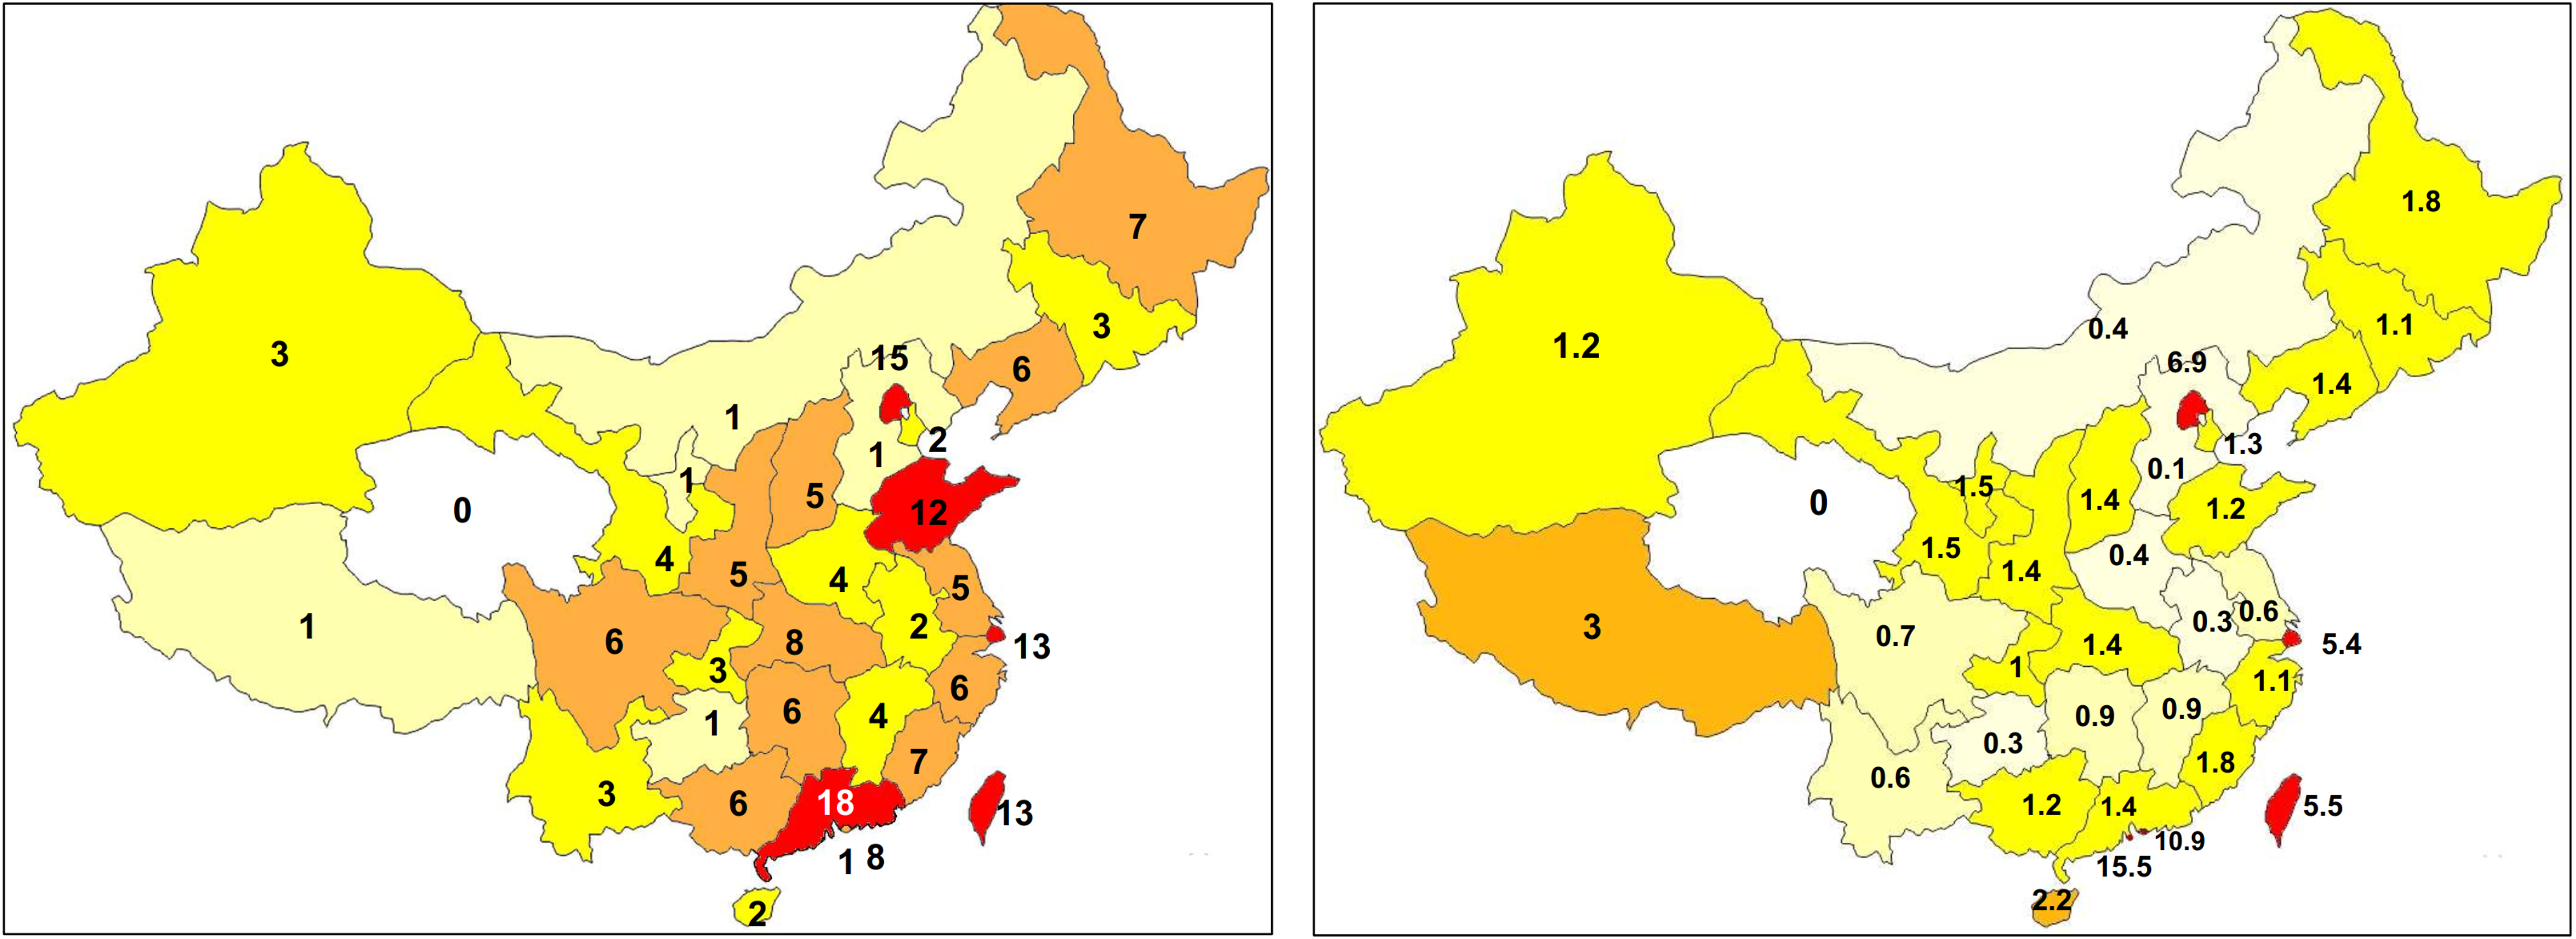
\includegraphics[width=0.9\textwidth]{0049.jpg}
      \bicaption{a) Number of cyclotrons for the production of medical radioisotopes by province, b) per 10 million people}{a) 各省用于生产医学放射性同位素的回旋加速器数量,b) 每千万人口的回旋加速器数量} \label{fig45}
\end{figure}

Yet, when we divide number of cyclotrons by population of each province then we see that the richest are Beijing, Hong Kong, Macau, Shanghai and Taiwan. They are at the European level and even higher. Most of other provinces are around one cyclotron per 10 million people, some are lower, but Xizang, with only one cyclotron comes much higher because of its quite small population. Obviously, China needs much more cyclotrons to close the gap with developed countries at least 4 times more than now.

然而,当我们考虑每个省回旋加速器数量与人口的比例时,显然,北京、香港、澳门、上海和台湾的比例最高,达到甚至超过欧洲水平。大多数其他省份的平均水平约为每1000万人一个回旋加速器,有些则更低。值得注意的是,西藏只有一个回旋加速器,但由于其较小的人口,导致其人均比例较高。显然,中国需要显著增加回旋加速器的数量,至少是现在的四倍,以缩小与发达国家之间的差距。

\subsection{Future of Radiopharmaceutical Chemistry\\放射药物化学的未来}

As nuclear medicine is making important advancements, it is also becoming more available and affordable. Medicinal cyclotrons were a rarity just a few decades ago, but now the number of producers is increasing, while important large medical centers can afford at least one radiochemical suite. Further automatization and artificial intelligence will make radiopharmaceutical suites fully automatic, especially for several main radiopharmaceuticals, increasing the availability of nuclear medicine procedures.  

随着核医学的不断进步,其可获得性和经济性也在提升。医疗回旋加速器在几年前还是一种稀有设备,现在制造商数量正在增加,重要的大型医疗中心至少可以配备一个放射化学实验室。未来,自动化程度将进一步提高,人工智能的应用将使放射药物实验室实现全自动化,特别是对于几种主要放射药物,从而提升核医学程序的可获得性。

In the future, some radioisotopes commonly made by reactors, like \(\mathrm{^{99m}Tc}\), will be made by cyclotrons only, although the importance of \(\mathrm{^{99m}Tc}\) and SPECT technology will continue to fade in favor of PET radionuclides. The main reason is that PET technology provides much clearer images with higher resolution.  

未来,一些传统由反应堆生产的放射性同位素,如${}^\text{99m}\text{Tc}$,可能会完全通过回旋加速器生产。然而,尽管${}^\text{99m}\text{Tc}$和SPECT技术的重要性可能会下降,PET放射性核素预计将变得更为重要。这一变化的主要原因在于PET技术能够提供更清晰、更高分辨率的图像。

We will see new, quicker, and more practical ways to synthesize radiopharmaceuticals: new reactions will be optimized by artificial intelligence. Novel methods in organic chemistry will come with faster and more yielding reactions suitable for automation. Also, we can predict the entrance of nanoscience and supramolecular chemistry into the area of radiopharmaceuticals.  

我们可以预见,合成放射药物的新方法将更快捷、更实用,新反应将通过人工智能进行优化。新型有机化学方法将带来更快速、更高产的反应,适合自动化。此外,纳米科学和超分子化学预计将逐步进入放射药物领域。

Automatic synthesis, purification, and formulation of radiopharmaceuticals will be improved, incorporating robotic technologies (compact production machines will be developed for the continuous production of radiotracer doses) and artificial intelligence.  

放射药物的自动合成、纯化和配制将得到改进,机器人技术将被引入,开发紧凑型生产设备以实现放射性示踪剂剂量的连续生产。

New radiotracers for PET imaging (in oncology, cardiology, neurology, infection, inflammation, and others) will be developed based on new very specific monoclonal antibodies, while targeted radioimmunotherapy with alpha emitters will be improved and expanded, possibly into the area of autoimmune diseases. The area of radioactive theranostics will also expand and become routine. Some exotic radionuclides, such as \(\mathrm{^{211}At}\), will become common. Radiotherapy will slowly but surely make its way into common and routine use.

新的PET成像示踪剂将被开发,针对肿瘤学、心脏病学、神经学、感染、炎症等多个应用领域,利用高度特异性的单克隆抗体。针对$\alpha$射线发射体的靶向放射免疫治疗预计将扩展,可能涉及自身免疫疾病领域。放射性治疗的综合诊疗领域也将扩大并变得常规化,${}^{211}\text{At}$等一些新型放射性同位素将变得更为常见。

Ultimately, radiotherapy is poised to transition into common, routine use, marking a significant advancement in the application of radiopharmaceuticals in medical practice.

最终,放射治疗有望转变为常规、日常使用,标志着放射药物在医学实践中应用的重要进步。

\newpage

\section{\mbox{Chapter III : Key Concepts in (Radio)pharmacology and (Radio)pharmaceuticals}\\第三章 —— (放射)药理学与(放射)药物的关键概念}

\subsection{What Would Be an Ideal Medical Radionuclide?\\理想的医学放射性核素应具备什么特征?}


The key elements in radiopharmaceuticals are radionuclides. However, not all radionuclides can be used for medicinal purposes. In fact, most of the nuclides from the nuclear power area cannot be used in the medical area. What would be an ideal radionuclide?

放射药物的关键成分是放射性核素。然而,并不是所有放射性核素都可以用于医学目的。事实上,大多数来自核电领域的核素不能在医学领域使用。理想的放射性核素应具备什么特征?

There are some requirements a radionuclide has to fulfil to be considered as good for medical applications.

放射性核素需要满足一些要求,才能被认为适合医学应用。

\begin{itemize}


      \item A good medical nuclide has to have a sufficiently short half-life. This is to avoid any unwanted accumulation in the organism. Half-life should be such that it is in minutes, hours, or days—definitely not in months or years. But, neither in seconds—too short a half-life is not practical. Therefore, we cannot use long-lived radionuclides such as \(\mathrm{^{238}U}\), \(\mathrm{^{235}U}\), \(\mathrm{^{232}Th}\), \(\mathrm{^{226}Ra}\), \(\mathrm{^{60}Co}\), nor can we use radionuclides with too short a half-life such as \(\mathrm{^{15}C}\), or \(\mathrm{^{212}Ra}\).


            一种好的医学核素必须具有足够短的半衰期。这是为了避免在机体内产生不必要的积累。半衰期应为几分钟、几小时或几天,绝对不能是几个月或几年。但也不能是几秒钟——半衰期过短是不实用的。因此,我们不能使用长寿命的放射性核素,如${}^\text{238}\text{U}$、${}^\text{235}\text{U}$、${}^\text{232}\text{Th}$、${}^\text{226}\text{Ra}$、${}^\text{60}\text{Co}$,也不能使用半衰期过短的核素,如${}^\text{15}\text{C}$或${}^\text{212}\text{Ra}$。


      \item Medical radionuclide has to have sufficiently high specific activity so that it can be used as a tracer; its dose in grams should be negligible: also, specific activity has to be high to enable targeted radiotherapy to be achievable with very tiny amounts of material.

            医学放射性核素必须具有足够高的比活性,以便可以作为示踪剂使用;其剂量应微不足道:此外,比活性必须高,以使靶向放射治疗能够用极少量的材料实现。

      \item It needs to have high radionuclidic and radiochemical purity: it should be only one radioisotope of only one element. Therefore, radionuclides that are hard to be purified and usually contain radiotoxic radionuclides as impurity cannot be used.

            它需要具有高的放射性核素纯度和放射化学纯度:应仅为单一元素的单一放射性同位素。因此,难以纯化且通常含有放射毒性核素杂质的核素不能使用。

      \item Emission should be proper and should penetrate to some desirable distance: we cannot use ${}^\text{14}\text{C}$, for example, or ${}^\text{3}\text{H}$ since these radionuclides emit very weak beta particles that have no energy to penetrate more than several micrometers of tissue. Therefore, it would be impossible to detect them by their external irradiation on a live person.

            发射应适当,并能穿透一定距离:例如,我们不能使用${}^\text{14}\text{C}$或${}^\text{3}\text{H}$,因为这些放射性核素发射的$\beta$粒子非常微弱,没有足够的能量穿透超过几微米的组织。因此,通过对活体的外部辐射检测它们将是不可能的。

      \item It should not be a radiotoxic radionuclide: otherwise, we will end up with more harm than benefit to the patient. Therefore, radiotoxic radionuclides of plutonium or ${}^\text{241}\text{Am}$, ${}^\text{210}\text{Po}$, ${}^\text{90}\text{Sr}$, ${}^\text{137}\text{Cs}$, or ${}^\text{226}\text{Ra}$ cannot be used.

            它不应是放射毒性核素:否则,我们将给患者带来更多伤害而不是益处。因此,U、${}^\text{241}\text{Am}$、${}^\text{210}\text{Po}$、${}^\text{90}\text{Sr}$、${}^\text{137}\text{Cs}$或${}^\text{226}\text{Ra}$等放射毒性核素不能使用。


      \item And finally, it should be cheap, convenient, and readily available, which means its production should not be overly complicated, hard, and expensive.

            最后,它应该便宜、方便且易于获得,这意味着其生产不应过于复杂、困难和昂贵。


\end{itemize}

\subsection{How Do We Classify Radiopharmaceutical Agents?\\如何对放射性药物进行分类?}

There are numerous ways to do that, but here we will show examples of some common ways. Radiopharmaceutical agents can be classified based on the following categories:  

对放射性药物的分类有多种方法,以下是一些常见的分类方式。放射性药物可以根据以下类别进行分类:

\begin{itemize}


      \item Radioisotope they contain

            所含放射性同位素

      \item Emission they emit

            发射的辐射类型

      \item Chemical structure and/or pharmacological group they belong

            化学结构和/或药理学组别

      \item Therapeutic group or clinical use

            治疗组别或临床用途

\end{itemize}

Classification of radiopharmaceuticals \textbf{based on their radionuclide} is the most common type of classification. Based on this classification, we can say there are \(\mathrm{^{18}F}\)-containing radiopharmaceuticals, \(\mathrm{^{11}C}\)-containing radiopharmaceuticals, \(\mathrm{^{13}N}\), \(\mathrm{^{15}O}\), \(\mathrm{^{99m}Tc}\), radiocopper (\(\mathrm{^{64}Cu}\), \(\mathrm{^{67}Cu}\)), \(\mathrm{^{90}Y}\), radioiodine (\(\mathrm{^{123}I}\), \(\mathrm{^{125}I}\), \(\mathrm{^{131}I}\)), radio-gallium (\(\mathrm{^{68}Ga}\), \(\mathrm{^{67}Ga}\)), \(\mathrm{^{111}In}\), \(\mathrm{^{201}Tl}\)-containing radiopharmaceuticals, then those having lanthanides such as \(\mathrm{^{153}Sm}\), \(\mathrm{^{177}Lu}\), then those with heavy alpha emitters such as \(\mathrm{^{225}Ac}\), \(\mathrm{^{223}Ra}\), and finally, there are also radioactive noble gases \(\mathrm{^{133}Xe}\) and \(\mathrm{^{81m}Kr}\) that are used sometimes. However, there are more radioisotopes used for radiopharmaceuticals than are on this list.

\textbf{根据放射性核素}对放射性药物进行分类是最常见的分类方法。根据这种分类,我们可以说有含 ${}^\text{18}\text{F}$ 的放射性药物、含 ${}^\text{11}\text{C}$ 的放射性药物、${}^\text{13}\text{N}$、${}^\text{15}\text{O}$、${}^\text{99m}\text{Tc}$、放射性铜(${}^\text{64}\text{Cu}$、${}^\text{67}\text{Cu}$)、${}^\text{90}\text{Y}$、放射性碘(${}^\text{123}\text{I}$、${}^\text{125}\text{I}$、${}^\text{131}\text{I}$)、放射性镓(${}^\text{68}\text{Ga}$、${}^\text{67}\text{Ga}$)、${}^\text{111}\text{In}$、含 ${}^\text{201}\text{Tl}$ 的放射性药物,以及含镧系元素(如 ${}^\text{153}\text{Sm}$ 和 ${}^\text{177}\text{Lu}$)的放射性药物。此外,有时还使用 ${}^\text{225}\text{Ac}$ 和 ${}^\text{223}\text{Ra}$ 等重$\alpha$发射体以及 ${}^\text{133}\text{Xe}$ 和 ${}^\text{81m}\text{Kr}$ 等放射性惰性气体。然而,用于放射性药物的放射性同位素远不止这些。

\begin{table}[h]
      \centering
      \bicaption{Classification of radiopharmaceuticals based on their radioisotope}{基于放射性同位素的放射性药物分类} \label{tabel2}
      \begin{tabular}{cc}
      \toprule
      \textbf{Radioisotope} & \textbf{Radiopharmaceutical} \\
      \textbf{放射性同位素} & \textbf{放射性药物} \\
      \midrule
      \(\ce{^{18}F}\) & \(\ce{^{18}F}\)-Fluorodeoxyglucose, \(\ce{^{18}F}\)-Florbetapir, \(\ce{^{18}F}\)-Flumazenil, \(\ce{^{18}F}\)-Fluoroestradiol, 等 \\
      \(\ce{^{11}C}\) & \(\ce{^{11}C}\)-PIB, \(\ce{^{11}C}\)-Methionine, \(\ce{^{11}C}\)-DASB \\
      \(\ce{^{13}N}, \ce{^{15}O}\) & \(\ce{^{13}N}\) Ammonia, \(\ce{^{15}O}\) H2O \\
      \(\mathrm{^{99m}Tc}\) & \(\mathrm{^{99m}Tc}\)-Sestamibi, \(\mathrm{^{99m}Tc}\)-MDP, \(\mathrm{^{99m}Tc}\)-Mebrofenin, \(\mathrm{^{99m}Tc}\)-MAG3 \\
      \(\ce{^{64}Cu}, \ce{^{67}Cu}\) & \(\ce{^{64}Cu}\)-Dotatate, \(\ce{^{64}Cu}\)-ETS \\
      \(\ce{^{90}Y}\) & \(\ce{^{90}Y}\)-Ibritumomab tiuxetan \\
      \(\ce{^{123}I}, \ce{^{125}I}, \ce{^{131}I}\) & \(\ce{^{123}I}\)-NaI, \(\ce{^{131}I}\)-MIBG, \(\ce{^{131}I}\)-Tositumomab \\
      \(\ce{^{68}Ga}, \ce{^{67}Ga}\) & \(\ce{^{68}Ga}\)-DOTA-Octreotate \\
      \(\ce{^{111}In}\) & \(\ce{^{111}In}\)-Imciromab, \(\ce{^{111}In}\)-Pentetreotide, \(\ce{^{111}In}\)-Oxime \\
      \(\ce{^{201}Tl}\) & \(\ce{^{201}Tl}\)Cl \\
      \(\ce{^{153}Sm}, \ce{^{177}Lu}\) & \(\ce{^{153}Sm}\)-Lexidronam, \(\ce{^{177}Lu}\)-Oxodotreotide \\
      \(\ce{^{225}Ac}, \ce{^{223}Ra}\) & alpha emitters $\alpha$ 放射物 \\
      \(\ce{^{133}Xe}, \ce{^{81m}Kr}\) & noble gases 稀有气体  \\
      \bottomrule
      \end{tabular}
      \end{table}

\subsection{Another Way of Classifying Medical Radionuclides and Radiopharmaceuticals\\另一种分类医学放射性核素和放射药物的方法}

Another way of classifying medical radionuclides and radiopharmaceuticals is \textbf{based on the emissions they emit}: there are pure gamma emitters (these are decaying usually by electron capture, internal conversion, or just stabilization of isomers like in the case of \(\mathrm{^{99m}Tc}\)), then positron emitters, beta emitters, and alpha emitters. This classification actually coincides with clinical use classification: pure gammas are used in SPECT imaging, positrons in PET imaging, while betas and alphas are usually, but not only, therapeutic radionuclides.  

另一种分类医学放射性核素和放射药物的方法是根据它们\textbf{发射的辐射类型进行分类}。这包括纯$\gamma$发射体、正电子发射体、$\beta$发射体和$\alpha$发射体。这种分类与临床用途相吻合:纯$\gamma$射线用于SPECT成像,正电子用于PET成像,而$\beta$和$\alpha$通常是治疗用放射性核素。

\begin{itemize}

      \item \textbf{Pure Gammas ($\gamma$)}: ${}^\text{99m}\text{Tc}$, ${}^\text{123}\text{I}$, ${}^\text{125}\text{I}$, ${}^\text{201}\text{Tl}$, ${}^\text{111}\text{In}$, ${}^\text{67}\text{Ga}$, ${}^\text{81m}\text{Kr}$

            \textbf{纯$\gamma$射线}: ${}^\text{99m}\text{Tc}$、${}^\text{123}\text{I}$、${}^\text{125}\text{I}$、${}^\text{201}\text{Tl}$、${}^\text{111}\text{In}$、${}^\text{67}\text{Ga}$、${}^\text{81m}\text{Kr}$

      \item \textbf{Positrons ($\beta^+$)}: ${}^\text{18}\text{F}$, ${}^\text{11}\text{C}$, ${}^\text{13}\text{N}$, ${}^\text{15}\text{O}$, ${}^\text{64}\text{Cu}$, ${}^\text{68}\text{Ga}$, ${}^\text{82}\text{Rb}$, ${}^\text{89}\text{Zr}$, ${}^\text{124}\text{I}$

            \textbf{正电子 ($\beta^+$)}: ${}^\text{18}\text{F}$、${}^\text{11}\text{C}$、${}^\text{13}\text{N}$、${}^\text{15}\text{O}$、${}^\text{64}\text{Cu}$、${}^\text{68}\text{Ga}$、${}^\text{82}\text{Rb}$、${}^\text{89}\text{Zr}$、${}^\text{124}\text{I}$

      \item \textbf{Betas ($\beta^-$)}: ${}^\text{177}\text{Lu}$, ${}^\text{90}\text{Y}$, ${}^\text{131}\text{I}$, ${}^\text{67}\text{Cu}$, ${}^\text{133}\text{Xe}$, ${}^\text{32}\text{P}$, ${}^\text{153}\text{Sm}$, ${}^\text{188}\text{Re}$

            \textbf{$\beta$射线 ($\beta^-$)}: ${}^\text{177}\text{Lu}$、${}^\text{90}\text{Y}$、${}^\text{131}\text{I}$、${}^\text{67}\text{Cu}$、${}^\text{133}\text{Xe}$、${}^\text{32}\text{P}$、${}^\text{153}\text{Sm}$、${}^\text{188}\text{Re}$

      \item \textbf{Alphas ($\alpha$)}: ${}^\text{225}\text{Ac}$, ${}^\text{223}\text{Ra}$, ${}^\text{221}\text{At}$, ${}^\text{227}\text{Th}$, ${}^\text{212}\text{Pb}$

            \textbf{$\alpha$射线 ($\alpha$)}: ${}^\text{225}\text{Ac}$、${}^\text{223}\text{Ra}$、${}^\text{221}\text{At}$、${}^\text{227}\text{Th}$、${}^\text{212}\text{Pb}$

\end{itemize}

Third, we can classify all radiopharmaceuticals by using \textbf{chemo-pharmacological} classification, which means, based on what kind of molecule they are, based on their chemical nature and hence the way they interact with body structures such as receptors.  

第三,我们可以通过\textbf{化学药理}分类对所有放射药物进行分类,基于它们的化学性质及其与体内结构(如受体)的相互作用方式。

Here we can define labelled analogues of natural compounds that are anyway always present in our organism and are not foreign, for example, nutrients such as sugars (like glucose), amino acids or common hormones, neurotransmitters, vitamins labelled with a radioactive atom. For example, those are \(\mathrm{^{18}FDG}\), \(\mathrm{^{18}F}\)-estradiol, \(\mathrm{^{11}C}\)-methionine, radiocobalt-labelled vitamin B12, and others.  

在这里,我们可以定义自然化合物的标记类似物,这些化合物通常存在于我们的有机体中,例如营养物质(如葡萄糖)、氨基酸、激素、神经递质和维生素,这些物质被放射性原子标记。例如,包括${}^\text{18}\text{F}$DG、${}^\text{18}\text{F}$-雌二醇、${}^\text{11}\text{C}$-美托洛尔和放射性钴标记的维生素B${}_{12}$。


Then we have labelled analogues of various drugs such as \(\mathrm{^{18}F}\)-lorbetapir, \(\mathrm{^{18}F}\)-flumazenil, but also in this group, there are labelled small molecules that are usually not registered drugs but behave as drugs by specifically binding onto certain cellular structures in the human body (such as receptors). Some of them are even failed drugs that failed to find their way into clinical practice due to certain reasons, but their good binding onto specific cellular structures allows them to be used as tracers.  

然后,我们有各种药物的标记类似物,如${}^\text{18}\text{F}$lorbetapir和${}^\text{18}\text{F}$lumazenil。该组还包括标记的小分子,这些小分子通常不是注册药物,但通过特异性结合人身体内某些细胞结构(如受体)表现出药物的作用。其中一些甚至是未能进入临床实践的失败药物,尽管出于某种原因,但它们与特定细胞结构的良好结合使其可以用作示踪剂。

Then, there are labelled natural or artificial macromolecules such as proteins or peptides, for example, \(\mathrm{^{18}F}\)-neurotensin.

最后,还有标记的天然或人工大分子,例如蛋白质或肽,例如lorbetapir-神经肽。

Bioconjugates are more complicated and sophisticated forms of radiopharmaceutical agents, where usually a radio-metal is chelated within a chelating ligand and then the whole complex is conjugated with a large biomolecule, such as a protein or peptide. These are more sophisticated radiopharmaceuticals, such as \(\mathrm{^{90}Y}\)-ibritumomab tiuxetan or \(\mathrm{^{68}Ga}\)-DOTA-octreotate.  

生物结合物是放射药物的一种更复杂和精细的形式,通常是将放射性金属与配体螯合,然后与大分子生物分子(如蛋白质或肽)结合。例如,${}^\text{90}\text{Y}$-伊布利单抗注射剂或${}^\text{68}\text{Ga}$-DOTA-八肽等复杂的放射药物。


Then, there are various complexes and chelates or more simple complexes like \(\mathrm{^{99m}Tc}\)-sestamibi, \(\mathrm{^{99m}Tc}\)-MDP, \(\mathrm{^{99m}Tc}\)-DTPA.  

然后,还有各种复杂物和螯合物,以及更简单的复合物,如${}^\text{99m}\text{Tc}$-六氟化锝、${}^\text{99m}\text{Tc}$-MDP和${}^\text{99m}\text{Tc}$-DTPA。

Finally, old-style simple salts like NaI, NaTcO\(_4\), \(\mathrm{^{223}Ra}\)Cl\(_2\), \(\mathrm{^{89}Sr}\)Cl\(_2\), and \(\mathrm{^{82}Rb}\)Cl\(_2\) are still in use.  

最后,老式简单盐类如NaI、NaTcO4、${}^\text{223}\text{RaCl}_2$、${}^\text{89}\text{SrCl}_2$和${}^\text{82}\text{RbCl}_2$仍在使用。

Therefore, we can conclude the chemo-pharmacological classification:

因此,我们可以总结出化学药理分类:

\begin{itemize}

      \item Labeled analogues of natural biomolecules (sugars, amino acids, hormones, neurotransmitters): ${}^\text{18}\text{F}$DG, ${}^\text{18}\text{F}$-estradiol, ${}^\text{11}\text{C}$-methionine, ${}^\text{11}\text{C}$-dopamine…

            天然生物分子的标记类似物(糖、氨基酸、激素、神经递质):${}^\text{18}\text{F}$DG、${}^\text{18}\text{F}$-雌二醇、${}^\text{11}\text{C}$-美托洛尔、${}^\text{11}\text{C}$-多巴胺…

      \item Drug analogues (labeled drugs): ${}^\text{18}\text{F}$lorbetapir, ${}^\text{18}\text{F}$lumazenil, ${}^\text{11}\text{C}$-DASB is not a registered drug although it acts as a drug.

            药物类似物(标记药物):${}^\text{18}\text{F}$lorbetapir、${}^\text{18}\text{F}$lumazenil,${}^\text{11}\text{C}$-DASB虽然不是注册药物,但其作用类似药物。

      \item Labeled proteins or peptides: ${}^\text{18}\text{F}$-Neurotensin.

            标记的蛋白质或肽:${}^\text{18}\text{F}$-神经肽。

      \item Bioconjugates: ${}^\text{90}\text{Y}$-Ibritumomab tiuxetan, ${}^\text{68}\text{Ga}$-DOTA-octreotate.

            生物结合物:${}^\text{90}\text{Y}$-伊布利单抗注射剂、${}^\text{68}\text{Ga}$-DOTA-八肽。

      \item Chelates or simple complexes: ${}^\text{99m}\text{Tc}$-sestamibi, ${}^\text{99m}\text{Tc}$-MDP, ${}^\text{99m}\text{Tc}$-DTPA…

            螯合物或简单复合物:${}^\text{99m}\text{Tc}$-六氟化锝、${}^\text{99m}\text{Tc}$-MDP、${}^\text{99m}\text{Tc}$-DTPA…

      \item Simple salts: NaI, NaTcO4, ${}^\text{223}\text{RaCl}_2$, ${}^\text{89}\text{SrCl}_2$, ${}^\text{82}\text{RbCl}$, ${}^\text{201}\text{TlCl}$.

            简单盐类:NaI、NaTcO4、${}^\text{223}\text{RaCl}_2$、${}^\text{89}\text{SrCl}_2$、${}^\text{82}\text{RbCl}$、${}^\text{201}\text{TlCl}$。

\end{itemize}

Also, radiopharmaceuticals can be classified based on a test or area we want to investigate or cure, such as cancer, endocrine disorders (hormones), cardiovascular disorders (heart), neurological or psychological disorders (brain), or excretory organs such as kidneys, or we may focus on traumas or infections. This is a purely medical classification.  

此外,放射药物还可以根据我们想要研究或治疗的测试或领域进行分类,例如癌症、内分泌疾病(激素)、心血管疾病(心脏)、神经或心理疾病(大脑)、排泄器官(如肾脏),或创伤或感染。这是纯粹的医学分类。

And finally, we can classify radiopharmaceuticals and medical radionuclides by methods of application: there are radionuclides for imaging, like those for PET (all are positron emitters), and for SPECT (pure gamma emitters). For radiotherapy, beta or alpha emitters are used, and finally, some light radionuclides like \(\mathrm{^{3}H}\), \(\mathrm{^{14}C}\), \(\mathrm{^{32}P}\), \(\mathrm{^{33}P}\), \(\mathrm{^{35}S}\), \(\mathrm{^{45}Ca}\), and \(\mathrm{^{51}Cr}\) are used only for laboratory tests, not in live persons.

最后,我们可以根据应用方法对放射药物和医学放射性核素进行分类:用于成像的放射性核素,如用于PET的(均为正电子发射体)和用于SPECT的(纯$\gamma$发射体)。对于放射治疗,使用$\beta$或$\alpha$发射体。最后,一些轻核素如${}^\text{3}\text{H}$、${}^\text{14}\text{C}$、${}^\text{32}\text{P}$、${}^\text{33}\text{P}$、${}^\text{35}\text{S}$、${}^\text{45}\text{Ca}$和${}^\text{51}\text{Cr}$仅用于实验室测试,而不用于活体。

\begin{itemize}

      \item \textbf{For imaging成像用:}

            \begin{itemize}

                  \item PET:${}^\text{18}\text{F}$、${}^\text{11}\text{C}$、${}^\text{13}\text{N}$、${}^\text{15}\text{O}$、${}^\text{64}\text{Cu}$、${}^\text{68}\text{Ga}$、${}^\text{82}\text{Rb}$、${}^\text{89}\text{Zr}$、${}^\text{124}\text{I}$

                  \item SPECT:${}^\text{99m}\text{Tc}$、${}^\text{123}\text{I}$、${}^\text{125}\text{I}$、${}^\text{201}\text{Tl}$、${}^\text{111}\text{In}$、${}^\text{67}\text{Ga}$、${}^\text{81m}\text{Kr}$

            \end{itemize}

      \item \textbf{For therapy治疗用:}

            ${}^\text{225}\text{Ac}$、${}^\text{223}\text{Ra}$、${}^\text{221}\text{At}$、${}^\text{227}\text{Th}$、${}^\text{212}\text{Pb}$、${}^\text{177}\text{Lu}$、${}^\text{90}\text{Y}$、${}^\text{131}\text{I}$、${}^\text{67}\text{Cu}$、${}^\text{133}\text{Xe}$、${}^\text{32}\text{P}$、${}^\text{153}\text{Sm}$、${}^\text{188}\text{Re}$

      \item \textbf{For laboratory tests only仅用于实验室测试:}

            ${}^\text{3}\text{H}$、${}^\text{14}\text{C}$、${}^\text{32}\text{P}$、${}^\text{33}\text{P}$、${}^\text{35}\text{S}$、${}^\text{45}\text{Ca}$和${}^\text{51}\text{Cr}$。


\end{itemize}

\subsection{What is Pharmacology?\\什么是药理学?}

In short, pharmacology is a science about drugs, how drugs work, and how drugs behave in a living organism. This science is part of medical sciences, and it incorporates elements of chemistry, biochemistry, cell biology, and physiology. Pharmacology deals with molecular, cellular, and organ/systems mechanisms of drug action, including systems, receptors, and ligands in the body, signal transduction, cellular communication, molecular interactions, therapy, and medical applications. It also covers the fate of drugs in the body: absorption, distribution, metabolism, and excretion. Additionally, there is a section of pharmacology called clinical pharmacology, which focuses on the practical medical application of drugs, such as doses, indications, contraindications, side effects, etc.

简而言之,药理学是研究药物的科学,关注药物如何在活体内发挥作用和行为。该领域是医学科学的一部分,涉及化学、生物化学、细胞生物学和生理学的许多方面。药理学研究药物作用的分子、细胞和器官/系统机制,包括体内的系统、受体、配体、信号转导、细胞通信、分子相互作用、治疗和医学应用。它还探讨药物在体内的命运:吸收、分布、代谢和排泄。此外,还有一个称为临床药理学的部分,处理药物的实际医学应用,包括剂量、适应症、禁忌症和副作用。

Pharmacology generally consists of two main branches:

药理学一般包括两个主要分支:

\begin{itemize}

      \item Pharmacodynamics
            药效学

      \item Pharmacokinetics
            药代动力学

\end{itemize}
\subsubsection{What is Pharmacodynamics?什么是药效学?}

Pharmacodynamics deals with how a drug works at the cellular and molecular level. It covers the science of molecular, cellular, and organ/systems mechanisms of action, such as the molecular interactions of drugs with cellular structures, proteins, receptors, enzymes, and other ligands in the body. It answers questions about where and how a drug binds in the body or cell and how it produces its effect. It also deals with the (bio)chemistry of drug binding (ligand-drug interaction) and the doses (concentrations) of drugs required to trigger an effect.

药效学关注药物在细胞和分子水平上的作用。它涉及分子、细胞和器官/系统作用机制的科学,例如药物与细胞结构、蛋白质、受体、酶和其他配体之间的分子相互作用。它解决了药物在体内或细胞中的结合位置和方式,以及药物如何产生作用的问题。它还涉及药物结合的(生物)化学(配体-药物相互作用)以及触发效果所需的药物剂量(浓度)。

\begin{figure}[ht]
    \centering
    \includegraphics[width=0.9\textwidth]{0055.jpg}
    \bicaption{Pharmacodynamics deals with how drug interacts with tiny structures of cells at molecular level.}{药效学研究药物如何与细胞微小结构在分子层面相互作用} \label{fig46}
\end{figure}


\subsubsection{What is Pharmacokinetics?什么是药代动力学?}

The second branch of pharmacology, pharmacokinetics, deals with the question of how a drug travels through the body. What happens to a drug as it moves through the body before it reaches the site of action and after it leaves? It deals with absorption, distribution, metabolism, and finally excretion or elimination of drugs. In other words: how does the drug enter the body, how quickly does it act, where does it go, how long does it stay, what does it turn into, and how and how quickly does it leave the body? It also focuses on what happens to a drug in the liver and other tissues where it is metabolized, meaning chemically and biochemically modified or broken down.

药代学是药理学的第二个分支,研究药物如何在体内运输。药物在到达作用部位之前以及离开之后,体内发生了什么?它涉及药物的吸收、分布、代谢以及最终的排泄或消除。换句话说:药物是如何进入体内的,作用多快,去哪里,停留多久,转化为什么,以及如何以及多快地离开体内?它还关注药物在肝脏及其他代谢组织中发生的变化,意味着药物被化学和生化修饰或分解。

\subsubsection{How a Drug Travels Through the Body?药物如何在体内循环?}

\begin{figure}[ht]
    \centering
    \includegraphics[width=0.75\textwidth]{0056.jpg}
    \bicaption{a) Pharmacokinetics is dealing with the traffic of drug in human organism; b) routes for drug application in humans}{a) 药物代谢动力学研究药物在人体内的运动过程;b) 药物在人类体内的应用途径} \label{fig47}
\end{figure}

We can distinguish five stages of a drug pathway through the body: absorption, metabolism, distribution, elimination, and accumulation (Figure 47a). In absorption, we are interested in knowing how a drug enters the body and how quickly it is absorbed: what is the kinetics (how fast) of absorption? For example, if a drug is taken through the mouth, it will be absorbed either in the mouth, stomach, or intestines. After absorption, it first arrives in the liver where it is metabolized and only then enters the bloodstream. Absorption via mouth is usually slow to medium slow. Once a drug is in the liver, it gets metabolized, changed, and covalently modified. Distribution is a stage where we want to know where a drug goes, to which organ? Some drugs prefer certain organs, while it is hard to find them in some other organs. Some drugs cannot enter the brain (there is a special so-called “blood-brain barrier” only some drugs can enter the brain if these drugs are lipophilic enough). For example, iodine goes almost exclusively to the thyroid gland and is hardly found anywhere else. Distribution depends on pKa, lipophilicity, solubility, and other factors. Elimination (also known as excretion) is the removal of a drug from the organism: we wish to know parameters of the drug clearance, how and how quickly the drug is removed from the organism. Drugs are usually filtered out of the body in the kidneys, into urine, and via the bladder, they go out of our body. Another option is through the colon and feces after modification in the liver where the drug gets metabolized into a form that cannot be reabsorbed in the intestines. It is important to know that the human body has the ability to recognize what is a xenobiotic – a foreign substance that is possibly toxic and should not be in the organism, and then to get rid of it. Drugs are xenobiotics; they are foreign to our body. At the end, there is accumulation: some drugs tend to accumulate in the organism, usually in fatty tissue or quite often in bones. Drugs can be taken or applied in various ways, but the final goal is to get a drug into the bloodstream.  

我们可以区分药物在体内的五个阶段:吸收、代谢、分布、排泄和积累(图47a)。在吸收阶段,我们关心的是药物如何进入体内,以及它被吸收的速度:吸收的动力学(吸收速度)是什么?例如,如果药物是通过口服摄入的,它将在口腔、胃或肠道中被吸收。吸收后,药物首先到达肝脏,在肝脏中被代谢,只有在此之后才进入血液循环。通过口服的吸收通常较慢或中等慢。当药物进入肝脏后,它会被代谢、改变并发生共价修饰。分布阶段是我们想知道药物去向何处,去哪个器官?一些药物偏爱某些器官,而在一些其他器官中很难找到它们。有些药物无法进入大脑(大脑有一个特殊的“血脑屏障”,只有某些药物,如果它们足够亲脂性,才能进入大脑)。例如,碘几乎专门进入甲状腺,很难在其他地方找到。药物的分布取决于pKa、亲脂性、溶解性和其他因素。排泄(也叫排除)是药物从机体中去除的过程:我们希望了解药物清除的参数,药物是如何以及多快地从机体中被去除的。药物通常通过肾脏过滤排出体外,进入尿液,经过膀胱排出体外。另一种方式是通过结肠和粪便,在肝脏中药物被代谢成无法在肠道重新吸收的形式。重要的是要知道人体有能力识别外源性物质——可能有毒的外来物质并应当被排除在体外——然后将其去除。药物是外源物质,它们是我们体外的物质。最后是积累:一些药物倾向于在机体内积累,通常积累在脂肪组织或很常见地在骨骼中。药物可以通过多种方式摄入或应用,但最终的目标是将药物引入血液循环。

So, the most common way is to swallow it, through the mouth, like tablets or capsules. We call this the oral route. A drug gets dissolved in the stomach and gets absorbed in the stomach or intestines, then passes through the liver, and then enters the bloodstream. There is an option to avoid the stomach and get the drug directly into the bloodstream, using a needle! This is called parenteral application, usually through injection:

因此,最常见的方式是吞服药物,通过口腔,如片剂或胶囊。我们称之为口服途径。药物在胃中溶解,并在胃或肠道中被吸收,经过肝脏,然后进入血液循环。还有一种方式是避免胃肠道,直接通过针头将药物送入血液循环!这被称为外科应用,通常通过注射:


\begin{itemize}

      \item It can be directly into a vein (called intravenous),

            直接进入静脉(称为静脉注射),

      \item Into an artery (intra-arterial),

            进入动脉(动脉注射),

      \item Into a muscle (intramuscular),

            进入肌肉(肌肉注射),

      \item Below the skin (subcutaneous),

            皮下注射(皮下),

      \item A slow injection of a large volume of liquid into a vein (called infusion).

            大量液体缓慢注入静脉(称为输注)。

\end{itemize}

Another quick way of getting a drug into the bloodstream is by inhalation (through the lungs), and for that, a drug should be in the form of a spray or powder, or even a gas.Sometimes, a drug is given into the rectum and is then absorbed there (rectal application).There are other types of applications such as sublingual, where the drug is kept only in the mouth, then transdermal, where some very fatty drug gets absorbed into the bloodstream directly through the skin: this is usually very slow and rarely, via a patch, drug has to be very lipophilic and very potent (like fentanyl or some hormones).

另一种快速将药物输送入血液的方法是通过吸入(通过肺部),为此药物应该以喷雾、粉末或气体的形式存在。有时,药物通过直肠给药,并在此处被吸收(直肠应用)。还有其他类型的给药方式,例如舌下给药,药物只保留在口腔中;然后是经皮给药,某些脂溶性药物直接通过皮肤吸收到血液中:这通常非常缓慢,通常通过贴片给药,药物必须非常脂溶性且非常有效(如芬太尼或一些激素)。

\subsection{A Drug and Its Target\\药物及其靶标}

Here we are going to focus on the idea of a drug and its target. But what is a target in pharmacology?

在这里,我们将重点讨论药物及其靶标的概念。那么,药物靶标在药理学中是什么呢?

One cannot fully understand it if do not have some idea of how drug works and how it targets its target. A drug works by binding or interfering with its target or ligand in a live body. A target or a ligand is usually some particular cellular structure, a protein in most of the cases or sometimes (rarely) it can be a DNA. Only some anticancer drugs bind onto and disrupt DNA. Also, a target can be a biological structure not of a human, but of bacteria, virus or other microbes like in the case of antibiotics and antivirotics.

如果没有对药物如何作用及其如何靶向靶标的理解,就无法完全理解这一点。药物通过在活体内与其靶标或配体结合或干扰其作用。靶标或配体通常是某种特定的细胞结构,通常是蛋白质,或在某些情况下(很少)可以是DNA。只有一些抗癌药物能与DNA结合并破坏其结构。此外,靶标也可以是非人类的生物结构,如细菌、病毒或其他微生物,例如抗生素和抗病毒药物的靶标。

To list some examples based on its function, a targeted protein can be:

根据其功能列出一些例子,靶向蛋白可以是:
\begin{itemize}

      \item An enzyme: A drug can act as an inhibitor of an enzyme, and many drugs work in that way.

            酶:药物可以作为酶的抑制剂,许多药物以这种方式起作用。

      \item A receptor: Usually for some natural neurotransmitters or hormones, found on the surface of a cell but sometimes also inside the cell. A drug specifically binds to it and can activate or block its function.

            受体:通常是一些自然神经递质或激素,通常位于细胞表面,但有时也位于细胞内部。药物特异性地与之结合,可以激活或阻断其功能。

      \item An ion channel: For biological ions such as sodium, potassium, calcium; a drug can block it or keep it open longer.

            离子通道:用于生物离子如钠、钾、钙;药物可以阻止其作用或使其保持开放状态更长时间。

      \item A transporter protein: A drug can block the transport of neurotransmitters, hormones, or some other small molecules.

            转运蛋白:药物可以阻止神经递质、激素或其他小分子的转运。

      \item Signal transducer: A drug can block or mimic cellular signaling mechanisms.

            信号转导:药物可以阻断或模拟细胞信号传导机制。

\end{itemize}

In general, by binding to its target protein, a drug usually changes (or modulates) the normal function of that target protein and the whole cell. When the function of many cells is modulated, the whole tissue or organ is affected by the drug.

一般来说,药物通过与其靶标蛋白结合,通常会改变(或调节)该靶标蛋白及整个细胞的正常功能。当许多细胞的功能被调节时,整个组织或器官都会受到药物的影响。

This may sound like the binding of a metal and ligand in coordination chemistry, but there is a big difference! A metal usually binds many ligands, but one drug usually binds only one or very few targets: drug-target binding tends to be quite specific, just like in the case of hormones (hormones and neurotransmitters are, in fact, some kind of internal drugs).

这听起来可能像配位化学中金属与配体的结合,但两者之间有很大区别!金属通常会与多个配体结合,但一个药物通常只结合一个或很少几个靶标:药物与靶标的结合往往非常特异,就像激素的情况一样(激素和神经递质实际上是某种内部药物)。

\begin{figure}[ht]
    \centering
    \includegraphics[width=0.5\textwidth]{0058.jpg}
    \bicaption{Concept of drug and its target is similar like the concept of a key and the lock: one drug (key) can activate a target (lock) another drug (key) cannot: Drug A binds to receptor, while drug B cannot bind to receptor!}{药物及其靶点的概念类似于钥匙与锁的概念:一种药物(钥匙)可以激活靶点(锁),而另一种药物(钥匙)不能:药物A与受体结合,而药物B不能与受体结合!} \label{fig48}
\end{figure}

\begin{figure}[ht]
    \centering
    \includegraphics[width=0.5\textwidth]{0058[2].jpg}
    \bicaption{A drug binds onto its receptor (protein) through molecular recognition: topology of the drug fits into topology of the target!}{药物通过分子识别与其受体(蛋白质)结合:药物的拓扑结构与靶点的拓扑结构相匹配!} \label{fig49}
\end{figure}

A drug and its target look more like a key and its lock: a drug is like a key, while the target is the lock. And one key opens only one specific lock. How is this possible? Because a specific molecular structure (or shape, pattern) of a drug can bind only exactly complementary molecular structure (pattern) of just certain proteins. Therefore, one drug can bind onto very few proteins (targets): very specific drug will bind only one protein (target) out of thousands available! When one molecule perfectly complements into another and likes to bind it we call this a molecular recognition.

药物及其目标看起来更像是一把钥匙和一把锁:药物就像是一把钥匙,而目标则是锁。一把钥匙只能打开一把特定的锁。这怎么可能呢? 因为药物的特定分子结构(或形状、模式)只能与特定蛋白质的分子结构(模式)完全互补地结合。 因此,一种药物只能与极少数蛋白质(靶点)结合:在成千上万种可用的蛋白质(靶点)中,非常特殊的药物只能与一种蛋白质(靶点)结合!当一种分子与另一种分子完美互补并喜欢结合时,我们称之为分子识别。

Here are some examples! Acetylsalicylic acid (also known as Aspirin) or ibuprofen or paracetamol: all these molecules look different (Figure 50), but they all are binding and are blocking the same family of similar enzymes: they inhibit enzymes cyclooxygenases (COX-1 and COX-2). By doing so they are acting as painkillers, alleviate pain, and decrease body temperature. Therefore, enzymes cyclooxygenases are targets of aspirin, ibuprofen and paracetamol.

下面是一些例子!乙酰水杨酸(又称阿司匹林)或布洛芬或扑热息痛:所有这些分子看起来都不一样(图 50),但它们都在结合和阻断同一系列类似的酶:它们抑制环氧化酶(COX-1 和 COX-2)。这样,它们就能起到止痛、减轻疼痛和降低体温的作用。因此,环氧化酶是阿司匹林、布洛芬和扑热息痛的靶点。

\begin{figure}[ht]
    \centering
    \includegraphics[width=0.75\textwidth]{0059.jpg}
    \bicaption{When a drug binds onto enzyme and prevents its substrate to bind then it is called inhibitor of an enzyme – blocks its function. Such are famous and heavily used drugs like Aspirin, Paracetamol and Ibuprofen.}{当药物与酶结合并阻止其底物结合时,称为酶抑制剂——阻止其功能。这类药物包括著名且广泛使用的阿司匹林、扑热息痛和布洛芬。} \label{fig50}
\end{figure}
Here are some other, different examples (Figure 51): morphine, tramadol, methadone, and fentanyl. All these drugs have different structures but have something in common: these are all drugs that bind and activate the so-called $\mu$, $\delta$, and $\kappa$ opioid receptors in the brain. Since they are all binding and activating these receptors, we say they are all agonists (or activators) of $\mu$, $\delta$, and $\kappa$ opioid receptors in the brain.  

以下是一些不同的例子:吗啡、曲马多、美沙酮和芬太尼。这些药物的结构各不相同,但有一个共同点:它们都与大脑中的$\mu$、$\delta$和$\kappa$阿片受体结合并激活这些受体。由于它们都激活这些受体,我们称它们为$\mu$、$\delta$和$\kappa$阿片受体的激动剂(或激活剂)。

\begin{figure}[ht]
    \centering
    \includegraphics[width=0.75\textwidth]{0060.jpg}
    \bicaption{Agonist binds onto its receptor and activates – receptor triggers a cascade of reactor inside a cell or cellular compartment. Typical agonists are drugs like painkillers Fentanyl, Morphine, Methadone, and Tramadol.}{激动剂与其受体结合并激活——受体触发细胞或细胞区室内的一系列反应。典型的激动剂包括芬太尼、吗啡、美沙酮和曲马多等止痛药。} \label{fig51}
\end{figure}

Agonist is an activator: it binds a receptor and activates it. By doing so, these drugs are very strong painkillers, alleviate pain, but also cause euphoria, sedation, and addiction. Therefore, $\mu$, $\delta$, and $\kappa$ opioid receptors are targets of morphine, tramadol, methadone, and fentanyl.  

激动剂是激活剂:它与受体结合并激活它。通过这种方式,这些药物是非常强效的止痛药,缓解疼痛,同时也会导致愉悦感、镇静和成瘾。因此,$\mu$、$\delta$和$\kappa$阿片受体是吗啡、曲马多、美沙酮和芬太尼的靶标。

Some other drugs bind onto receptors but then are not activating them but are blocking them: atenolol, for example, binds and blocks the so-called $\beta$-receptors in blood vessels (we call these drugs $\beta$-antagonists or $\beta$-blockers, Figure 52). As a consequence, the natural neurotransmitter and hormone adrenaline cannot bind to these $\beta$-receptors, where $\beta$-antagonists such as atenolol “sit” on adrenaline’s place, and therefore atenolol lowers blood pressure and slows the heart rate.  

一些其他药物结合于受体,但并不激活它们,而是阻断它们。例如,阿莫洛尔(atenolol)结合并阻断血管中的所谓$\beta^{-}$受体(我们称这些药物为$\beta^{-}$拮抗剂或$\beta^{-}$阻滞剂)。因此,自然神经递质和激素肾上腺素无法结合这些$\beta^{-}$受体,因为$\beta^{-}$拮抗剂如阿莫洛尔“坐”在肾上腺素的位置上。因此,阿莫洛尔降低血压并减缓心率。

\begin{figure}[ht]
    \centering
    \includegraphics[width=0.75\textwidth]{0061.jpg}
    \bicaption{Some old drugs for treating cancer: they are reactive molecules that bind and destroy DNA}{一些治疗癌症的旧药物:它们是反应性分子,能够结合并破坏DNA} \label{fig52B}
\end{figure}

Haloperidol is another example of an antagonist. It binds and blocks the so-called $D_2$-receptors in the brain, normally reserved for the neurotransmitter dopamine. Dopamine then cannot bind $D_2$-receptors, and this helps to alleviate schizophrenia (therefore we call haloperidol an antipsychotic). A natural product from a poisonous plant, atropine binds and blocks M-receptors, where the neurotransmitter acetylcholine usually binds. Acetylcholine therefore cannot bind to M-receptors as long as atropine is bound to the receptors, taking acetylcholine’s natural position. Hence, it is used as a drug for bradycardia, and it also increases heart rate. In total, an antagonist or a blocker is a drug that binds to a receptor and blocks its function.

氟哌啶醇是另一个拮抗剂的例子。它结合并阻断大脑中所谓的$D_2$受体,通常这些受体是为神经递质多巴胺保留的。多巴胺因此无法结合$D_2$受体,这有助于缓解精神分裂症(因此我们称氟哌啶醇为抗精神病药物)。来自有毒植物的天然产物阿托品结合并阻断M受体,而通常神经递质乙酰胆碱会结合这些受体。乙酰胆碱因此无法结合M受体,只要阿托品占据了受体,乙酰胆碱的自然位置就被占据。因此,它被用作治疗心动过缓的药物,并且它也能增加心率。总的来说,拮抗剂或阻滞剂是指一种结合受体并阻断其功能的药物。

A natural product from a poisonous plant, atropine, binds and blocks $M$-receptors, where the neurotransmitter acetylcholine usually binds. Acetylcholine cannot bind to the $M$-receptors as long as atropine is bound to the receptors, taking acetylcholine’s natural position. Hence, it is used as a drug for bradycardia, and it also increases heart rate. In total, an antagonist or a blocker is a drug that binds to a receptor and blocks its function.

来自一种有毒植物的天然产物阿托品(atropine)结合并阻断$M$-受体,而神经递质乙酰胆碱通常结合在这些受体上。只要阿托品与受体结合,乙酰胆碱就无法结合到$M$-受体,从而占据了乙酰胆碱的自然位置。因此,它被用作治疗心动过缓的药物,并且也能增加心率。总之,拮抗剂或阻滞剂是指结合受体并阻断其功能的药物。

Only certain drugs bind DNA. For example, some old-style anticancer drugs covalently bind DNA and damage it permanently, causing the death of cells that multiply a lot (like cancer cells). We call these drugs “alkylating agents”. However, these drugs are not very specific, causing many side effects, some of which are very nasty and hard to withstand. The effect of these drugs is somewhat similar to the effect of ionizing radiation.  

只有某些药物能够与DNA结合。例如,一些传统的抗癌药物通过共价结合DNA并永久性地损伤它,导致大量增殖的细胞(如癌细胞)死亡。我们将这些药物称为“烷基化剂”。然而,这些药物并不具备很高的特异性,导致许多副作用,其中一些副作用非常严重且难以忍受。这些药物的作用与电离辐射的作用有些相似。  

What are the factors that influence drug behavior? First and foremost, it is the chemical and molecular structure of a drug (shape, topology, charge density) that directs the pharmacological effect of a drug. The pharmacodynamics of a drug depends on its molecular structure. Other factors include the solubility of the drug in water (drugs should be soluble in water at least a bit), its $pK_a$ (ionization has a huge influence on the behavior of drugs), and how lipophilic it is. For example, more lipophilic molecules are able to cross cell membranes and arrive at the site of action. In general, the behavior of a drug is an interplay between molecular structure, solubility, $pK_a$, lipophilicity, and some other factors.

影响药物行为的因素有哪些?首先,药物的化学结构和分子结构(形状、拓扑结构、电荷密度)决定了药物的药理作用。药物的药效学取决于其分子结构。其他因素包括药物在水中的溶解度(药物至少应在水中有一点溶解度)、药物的 $pK_a$(电离对药物的行为有很大影响)以及药物的亲脂性。例如,亲脂性更强的分子能够穿过细胞膜到达作用部位。一般来说,药物的行为是分子结构、溶解度、$pK_a$、亲脂性和其他一些因素之间的相互作用。

\subsection{Doses in pharmacology and radio(pharmacology)\\药理学与放射药理学中的剂量}

As we have seen one target can be targeted by several drugs. On the other hand, drugs that have only one target are called “specific” and have fewer side effects. However, very specific drugs are quite rare, most of drugs have not only one target, but several: more targets a drug has less specific it is and has more side effects. Each drug binds to its target with a specific affinity ($K_1$):

我们看到,一个靶点可以被多种药物靶向。另一方面,仅有一个靶点的药物被称为“特异性药物”,并且副作用较少。然而,真正特异的药物非常稀少,大多数药物不仅有一个靶点,而是有多个:药物靶点越多,药物的特异性就越低,副作用就越多。每种药物以特定的亲和力($K_1$)与其靶点结合:

$$ [D] + [R] \xrightleftharpoons[K_2]{K_1} [DR]$$


This is an equivalent of binding affinity in coordination chemistry. The specific affinity depends of molecular structure of a drug.

这相当于配位化学中的结合亲和力。特定亲和力依赖于药物的分子结构。

However, the total pharmacological effect of a drug (sometimes expressed as ED50) depends much on concentration of a drug in the proximity of the target: the smallest amount of drug you imagine does binds to its target but, however, to achieve measurable pharmacological effect a drug has to reach certain concentration: this is called a therapeutic concentration! In order drug to have its effect molecules of drug need to fill certain number of receptors. There is also something called potency: a drug that is causing the same pharmaceutical effect with lower therapeutic concentration is more potent, stronger.

然而,药物的总药理效应(有时表示为ED50)在很大程度上依赖于药物在靶点附近的浓度:你想象的最小药物量确实与其靶点结合,但要实现可测量的药理效应,药物必须达到某种浓度:这被称为治疗浓度!为了让药物产生效应,药物分子需要占据一定数量的受体。还有一种叫做效力的概念:一种药物如果能在较低的治疗浓度下引起相同的药理效应,则其效力更强。

Doses in pharmacology are usually at the range from 1000 mg to 1 mg. If evenly distributed throughout a live average human body (5 L) it can reach concentration of about 200 mg/L to 0.2 mg/L, and in most of the cases it is from 1 mM down to tens of nM. This is a usual pharmacological therapeutic range (Figure 53).

在药理学中,剂量通常在1000毫克到1毫克之间。如果均匀分布在一个平均人的身体(5升)中,其浓度可以达到大约200毫克/升到0.2毫克/升,在大多数情况下,从1毫摩尔降到几十纳摩尔。这是通常的药理治疗范围(图53)。

However, if the dose is too low then there will be no pharmacological effect at all, a patient does now feel any effect, nor any effect can be measured or observed. Yet, the small number of molecules of drugs that reach its targets do bind onto receptors but not in sufficient numbers.

然而,如果剂量过低,那么就不会产生任何药理效应,患者不会感受到任何效应,也无法测量或观察到任何效应。然而,少量达到靶点的药物分子确实会与受体结合,但数量不足。

If dose is too high then it is not good either: too much side effects, or it can be overdose, and if dose is very, very high a drug becomes a poison! Drug works the best in an optimal dose, so called therapeutic dose: just about to have a proper effect, but not side effects and not to be toxic. This is called a therapeutic window and sometimes tends to be quite narrow.

如果剂量过高,那么也不好:副作用过多,可能会出现药物过量,如果剂量非常非常高,药物就变成了毒药!药物在最佳剂量下效果最好,这被称为治疗剂量:刚好有适当的效果,但没有副作用且不具毒性。这被称为治疗窗口,有时可能相当窄。
\begin{figure}[ht]
    \centering
    \includegraphics[width=0.75\textwidth]{0062.jpg}
    \bicaption{With the increase of its dose the effect of a drug goes from therapeutic into toxic, it can be a drug or a poison depending on its dose. Yet, in nuclear medicine dose of radioactive drug (tracer) are far less than those required to make any physiological or pharmacological effect.}{随着药物剂量的增加,其效果从治疗性转变为毒性,它可以是药物,也可以是毒物,这取决于剂量。然而,在核医学中,放射性药物(示踪剂)的剂量远低于产生任何生理或药理效应所需的剂量。} \label{fig53}
\end{figure}


In nuclear medicine and especially in the area of nuclear imaging we want radiotracer molecule to bind onto its target and sends us its gamma-signal, but we do not want any pharmacological effect.

在核医学,尤其是在核成像领域,我们希望放射性示踪剂分子与其靶点结合并向我们发送$\gamma$信号,但我们不希望有任何药理效应。

And this is why in nuclear medicine doses of radiopharmaceuticals are actually much lower than in classic pharmacological therapy; doses in nuclear imaging are in the area where drug has no pharmacological effect whatsoever (Figure 53): it binds receptors but exerts no effect, dose is too small.

这就是为什么在核医学中,放射药物的剂量实际上远低于经典药物治疗的原因;在核成像中,剂量处于没有药理效应的范围内(图53):它结合受体,但没有任何效应,剂量过小。

Radiopharmaceutical doses are in MBq and mSv but if one recalculates them into molarity then it is at pM and nM levels, significantly lower than the doses in pharmacology.

放射药物的剂量以MBq和mSv为单位,但如果将其换算为摩尔浓度,则在pM和nM水平上,显著低于药理学中的剂量。

In fact, radiopharmaceuticals are often called tracers not drugs, especially when applied for imaging: De Hevesy tracer principle says that radiopharmaceuticals can participate in biological processes but should not alter or perturb them! This is the reason concentration of radiopharmaceutical in organism \underline{has to be much more below those that are typical for therapeutic dose}: just to bind the target, not to activate, not to inhibit, not to block it!

实际上,放射药物通常被称为示踪剂,而不是药物,特别是在成像应用时:德·赫维西示踪剂原理指出,放射药物可以参与生物过程,但不应改变或干扰它们!这就是放射药物在生物体内的浓度必须远低于治疗剂量的典型水平的原因:只是为了结合靶点,而不是激活、抑制或阻断它!

On the other hand, if applied for targeted radiation therapy (TRT) radiotherapeutic concentrations of radiopharmaceuticals are often smaller than pharmaceutical: radiation dose has to be high enough to kill all targeted cells, but low enough not to cause any unwanted radiation damage to healthy tissues.

另一方面,如果用于靶向放射治疗(TRT),放射药物的治疗浓度通常小于药物:辐射剂量必须足够高,以杀死所有靶向细胞,但又必须足够低,以免对健康组织造成任何不必要的辐射损伤。

\subsubsection{Doses in Imaging vs. Doses in Targeted Therapy 成像剂量与靶向治疗剂量}

It is important to remember that doses of radiopharmaceuticals are expressed in MBq, while the dose of ionising radiation received by a patient or targeted cells is in mSv or Sv (Sieverts).

重要的是要记住,放射药物的剂量以兆贝可(MBq)为单位,而患者或靶向细胞接收到的电离辐射剂量则以毫西弗(mSv)或西弗(Sv)为单位。

However, there is a big difference between imaging and therapy: imaging requires lower tracer doses, about 1-400 MBq (giving a patient a total of just a few mSv per dose). For example, the typical dose of FDG is from 200 to 400 MBq, and a patient receives from 4 to 8 mSv – that is acceptable. But its dose in grams is just 1 ng, which is a very, very tiny amount. Here are some other examples: \(\mathrm{{}^{99m}Tc}\)-sestamibi, a typical radiopharmaceutical for kidney function tests, is given at a dose of 150 to 740 MBq and gives the patient about 1.2-6 mSv. But the weight of this agent given to a patient is just 30 ng! Similarly, \(\ce{^{18}F}\)-estradiol, used for the diagnosis of breast cancer, is given at a dose of 185 MBq, delivering just 4 mSv to the patient, and the amount is a minute 0.845 ng.

然而,影像学与治疗之间有很大的差异:影像学需要较低的示踪剂剂量,大约1-400 MBq(每剂量给予患者的辐射总量仅为几mSv)。例如,典型的FDG剂量为200到400 MBq,患者接受的辐射剂量为4到8 mSv——这是可以接受的。但其克数剂量仅为1 ng,这是一个非常非常微小的数量。还有其他几个例子:\(\mathrm{{}^{99m}Tc}\)-sestamibi,一种用于肾功能检查的典型放射药物,剂量为150到740 MBq,给予患者的辐射剂量约为1.2-6 mSv。但这剂量给予患者的药物重量仅为30 ng!类似地,\(\ce{^{18}F}\)-estradiol用于乳腺癌诊断,剂量为185 MBq,给予患者的辐射剂量仅为4 mSv,剂量仅为0.845 ng。

On the other hand, targeted radiation therapy requires large doses (from 1 to several GBq), while the targeted cells receive lethal doses up to 30 Sv! For example, the therapeutic dose of 90Y-Ibritumomab tiuxetan is up to 1.2 GBq – targeted lymphoma cells receive a lethal dose of 17 Sv! What would happen if a person received a whole-body dose of 17 Sv? That person would immediately die. But in fact, the whole-body dose in targeted radiotherapy regimens is much lower, while 17 Sv is delivered only to the targeted malignant cells that need to be destroyed. Likewise, the therapeutic dose of 131I-Tositumumab is 3 GBq, and the lymphoma cells are hit with a devastating 27 Sv and killed, while the whole body gets just a few mSv and remains unharmed.


另一方面,靶向放射治疗需要较大剂量(从1到几GBq),而靶向细胞接受的致死剂量可高达30 Sv!例如,治疗剂量90Y-Ibritumomab tiuxetan可高达1.2 GBq——靶向的淋巴瘤细胞接收到17 Sv的致死剂量!如果一个人全身接受17 Sv的剂量会发生什么?那个人会立即死亡。但实际上,在靶向放射治疗方案中,全身剂量要低得多,17 Sv的剂量仅施加在需要摧毁的靶向恶性细胞上。类似地,131I-Tositumumab的治疗剂量为3 GBq,淋巴瘤细胞被击中致命的27 Sv并被杀死,而全身仅接收到几mSv且保持无害。


\subsection{Effect of Ionizing Radiation\\电离辐射的影响}
Is there some damaging effect of radiopharmaceuticals due to ionising radiation? As we know, radiopharmaceuticals are radioactive materials, and emit ionising radiation that can damage tissues. This negative side-effect is not incredibly significant in the radiopharmaceutical agents for imaging but tends to be more significant in targeted radiotherapy. As we know, beta and alpha particles can directly ionise biological structures and damage them, while gamma radiation primarily ionises water, and then this ionisation of water causes radiolysis and the generation of free radicals. These free radicals then react with biomolecules and cause damage (Figure 54).

放射药物是否会因电离辐射而造成损害?正如我们所知,放射药物是放射性物质,能够发射电离辐射并对组织造成损害。这一负面副作用在用于成像的放射药物中并不特别显著,但在靶向放射治疗中则更为重要。我们知道,$\beta$粒子和$\alpha$粒子可以直接电离生物结构并对其造成损害,而$\gamma$辐射则主要是电离水,进而导致水的电离引发辐射分解并生成自由基。这些自由基随后与生物分子反应并造成损害(图54)。

Toxicology is a science about poisons, while radiotoxicology is the science about the toxicity of a radioactive substance, where one looks primarily into the toxic effects of radioactive materials and their ionising radiation inside the human body, and the damage it causes to the body. It is different from classic toxicology, which deals only with chemical toxicity: radiotoxicity deals mainly with the toxic effects of ionising radiation! As mentioned earlier, radiotoxicology is less important in imaging due to very low doses, but more important in targeted radiation therapy (TRT): if the radionuclide is fully delivered just onto the target, then the overall radiotoxicity to the whole body could be low, since only the targeted tissue is affected. Some radiotoxicity at the place of entrance (vein, infusion) is of concern. However, the general rule is that a radiopharmaceutical agent should not be radiotoxic and should overall not cause harm!

毒理学是研究毒物的科学,而放射毒理学是研究放射性物质毒性的科学,主要关注放射性物质及其电离辐射在人体内的毒性作用,以及它对人体造成的损害。它不同于经典毒理学,后者仅处理化学毒性:放射毒理学主要处理电离辐射的毒性作用!如前所述,由于剂量非常低,放射毒理学在成像中的重要性较小,但在靶向放射治疗(TRT)中更为重要:如果放射性核素完全靶向目标部位,那么对全身的总体放射毒性可能较低,因为只有靶向组织受到影响。在进入部位(静脉、输注处)可能会有一定的放射毒性。然而,一般规则是,放射药物不应具有放射毒性,整体上不应造成伤害!

\begin{figure}[ht]
    \centering
    \includegraphics[width=0.5\textwidth]{0064.jpg}
    \bicaption{Gamma radiation ionises water and then reactive species (free radicals) are created that are ionising DNA, hence destruction of DNA with gamma radiation is indirect.}{伽马辐射电离水分子,进而生成反应性物质(自由基),这些自由基会电离DNA,因此伽马辐射引起的DNA破坏是间接的。} \label{fig54}
\end{figure}


\subsection{What are Theranostics?\\什么是治疗诊断学?}

It is also especially important to introduce the concept of theranostics. What are theranostics? They are agents that are both therapeutics and diagnostics at the same time! The name, as you can see, comes from combining “thera” (the first part of the word “therapeutic”) and “nostic” (the last part of the word “diagnostic”). How is this possible?

同样,介绍治疗诊断学的概念也尤为重要。什么是治疗诊断学?它们是同时具有治疗作用和诊断作用的药物!这个名称,如你所见,来自于将“thera”(“治疗性”一词的前半部分)和“nostic”(“诊断性”一词的后半部分)组合起来。这个概念是如何实现的呢?

We can imagine a radiopharmaceutical agent that is both an imaging agent and a targeted radiotherapeutic agent at the same time. For example, a radiopharmaceutical agent can contain a radionuclide with both \(\beta\)- and \(\gamma\) emission: the \(\beta\)-particle kills a cell, while the accompanying \(\gamma\)-ray serves as a location signal. These can be radionuclides such as \(\mathrm{^{177}Lu}\) or \(\mathrm{^{131}I}\) (Figure 55). Another concept is to have a radiopharmaceutical with two radionuclides, one alpha, and another gamma, where the alpha-emitting radionuclide delivers the therapeutic effect, while the gamma-emitting one serves to send an imaging signal from the site of therapy.


我们可以想象一个放射药物,它既是成像剂,又是靶向放射治疗剂。例如,放射药物可以包含一种既有\(\beta\)-射线又有\(\gamma\)-射线的放射性核素:\(\beta\)-粒子杀死细胞,而伴随的\(\gamma\)-射线则作为定位信号。这些核素可以是\(\mathrm{^{177}Lu}\)或\(\mathrm{^{131}I}\)(图55)。另一种概念是使用两种放射性核素,一种是$\alpha$射线,另一种是$\gamma$射线,其中$\alpha$射线发射核素提供治疗效应,而$\gamma$射线发射核素则用来从治疗部位发送成像信号。


\subsection{What Would Be an Ideal Medical Radionuclide?\\理想的医学放射性核素应具备什么特征?}


The key elements in radiopharmaceuticals are radionuclides. However, not all radionuclides can be used for medicinal purposes. In fact, most of the nuclides from the nuclear power area cannot be used in the medical area. What would be an ideal radionuclide?

放射药物的关键成分是放射性核素。然而,并不是所有放射性核素都可以用于医学目的。事实上,大多数来自核电领域的核素不能在医学领域使用。理想的放射性核素应具备什么特征?

There are some requirements a radionuclide has to fulfil to be considered as good for medical applications.

放射性核素需要满足一些要求,才能被认为适合医学应用。

\begin{itemize}


      \item A good medical nuclide has to have a sufficiently short half-life. This is to avoid any unwanted accumulation in the organism. Half-life should be such to be in minutes, hours, days, definitely not in months, or years. But, neither in seconds – a too short half-life is not practical. Therefore, we cannot use long-lived radionuclides such as ${}^\text{238}\text{U}$, ${}^\text{235}\text{U}$, ${}^\text{232}\text{Th}$, ${}^\text{226}\text{Ra}$, ${}^\text{60}\text{Co}$ nor can we use radionuclides with too short half-life such as ${}^\text{15}\text{C}$, or ${}^\text{212}\text{Ra}$.

            一种好的医学核素必须具有足够短的半衰期。这是为了避免在机体内产生不必要的积累。半衰期应为几分钟、几小时或几天,绝对不能是几个月或几年。但也不能是几秒钟——半衰期过短是不实用的。因此,我们不能使用长寿命的放射性核素,如${}^\text{238}\text{U}$、${}^\text{235}\text{U}$、${}^\text{232}\text{Th}$、${}^\text{226}\text{Ra}$、${}^\text{60}\text{Co}$,也不能使用半衰期过短的核素,如${}^\text{15}\text{C}$或${}^\text{212}\text{Ra}$。


      \item Medical radionuclide has to have sufficiently high specific activity so that it can be used as a tracer; its dose in grams should be negligible: also, specific activity has to be high to enable targeted radiotherapy to be achievable with very tiny amounts of material.

            医学放射性核素必须具有足够高的比活性,以便可以作为示踪剂使用;其剂量应微不足道:此外,比活性必须高,以使靶向放射治疗能够用极少量的材料实现。

      \item It needs to have high radionuclidic and radiochemical purity: it should be only one radioisotope of only one element. Therefore, radionuclides that are hard to be purified and usually contain radiotoxic radionuclides as impurity cannot be used.

            它需要具有高的放射性核素纯度和放射化学纯度:应仅为单一元素的单一放射性同位素。因此,难以纯化且通常含有放射毒性核素杂质的核素不能使用。

      \item Emission should be proper and should penetrate to some desirable distance: we cannot use ${}^\text{14}\text{C}$, for example, or ${}^\text{3}\text{H}$ since these radionuclides emit very weak beta particles that have no energy to penetrate more than several micrometers of tissue. Therefore, it would be impossible to detect them by their external irradiation on a live person.

            发射应适当,并能穿透一定距离:例如,我们不能使用${}^\text{14}\text{C}$或${}^\text{3}\text{H}$,因为这些放射性核素发射的$\beta$粒子非常微弱,没有足够的能量穿透超过几微米的组织。因此,通过对活体的外部辐射检测它们将是不可能的。

      \item It should not be a radiotoxic radionuclide: otherwise, we will end up with more harm than benefit to the patient. Therefore, radiotoxic radionuclides of plutonium or ${}^\text{241}\text{Am}$, ${}^\text{210}\text{Po}$, ${}^\text{90}\text{Sr}$, ${}^\text{137}\text{Cs}$, or ${}^\text{226}\text{Ra}$ cannot be used.

            它不应是放射毒性核素:否则,我们将给患者带来更多伤害而不是益处。因此,U、${}^\text{241}\text{Am}$、${}^\text{210}\text{Po}$、${}^\text{90}\text{Sr}$、${}^\text{137}\text{Cs}$或${}^\text{226}\text{Ra}$等放射毒性核素不能使用。


      \item And finally, it should be cheap, convenient, and readily available, which means its production should not be overly complicated, hard, and expensive.

            最后,它应该便宜、方便且易于获得,这意味着其生产不应过于复杂、困难和昂贵。


\end{itemize}

\subsection{How Do We Classify Radiopharmaceutical Agents?\\如何对放射性药物进行分类?}

There are numerous ways to classify radiopharmaceutical agents, but here we will show examples of some common methods. Radiopharmaceutical agents can be classified based on the following categories:
对放射性药物的分类有多种方法,以下是一些常见的分类方式。放射性药物可以根据以下类别进行分类:

\begin{itemize}


      \item Radioisotope they contain

            所含放射性同位素

      \item Emission they emit

            发射的辐射类型

      \item Chemical structure and/or pharmacological group they belong

            化学结构和/或药理学组别

      \item Therapeutic group or clinical use

            治疗组别或临床用途

\end{itemize}

Classification of radiopharmaceuticals \textbf{based on their radionuclide} is the most common type of classification. Based on this classification, we can say there are ${}^\text{18}\text{F}$-containing radiopharmaceuticals, ${}^\text{11}\text{C}$-containing radiopharmaceuticals, ${}^\text{13}\text{N}$, ${}^\text{15}\text{O}$, ${}^\text{99m}\text{Tc}$, radiocopper (${}^\text{64}\text{Cu}$, ${}^\text{67}\text{Cu}$), ${}^\text{90}\text{Y}$, radioiodine (${}^\text{123}\text{I}$, ${}^\text{125}\text{I}$, ${}^\text{131}\text{I}$), radio-gallium (${}^\text{68}\text{Ga}$, ${}^\text{67}\text{Ga}$), ${}^\text{111}\text{In}$, ${}^\text{201}\text{Tl}$-containing radiopharmaceuticals, as well as those having lanthanides such as ${}^\text{153}\text{Sm}$ and ${}^\text{177}\text{Lu}$. There are also heavy alpha emitters like ${}^\text{225}\text{Ac}$ and ${}^\text{223}\text{Ra}$, and radioactive noble gases like ${}^\text{133}\text{Xe}$ and ${}^\text{81m}\text{Kr}$ that are sometimes used. However, there are more radioisotopes used for radiopharmaceuticals than are on this list.

\textbf{根据放射性核素}对放射性药物进行分类是最常见的分类方法。根据这种分类,我们可以说有含 ${}^\text{18}\text{F}$ 的放射性药物、含 ${}^\text{11}\text{C}$ 的放射性药物、${}^\text{13}\text{N}$、${}^\text{15}\text{O}$、${}^\text{99m}\text{Tc}$、放射性铜(${}^\text{64}\text{Cu}$、${}^\text{67}\text{Cu}$)、${}^\text{90}\text{Y}$、放射性碘(${}^\text{123}\text{I}$、${}^\text{125}\text{I}$、${}^\text{131}\text{I}$)、放射性镓(${}^\text{68}\text{Ga}$、${}^\text{67}\text{Ga}$)、${}^\text{111}\text{In}$、含 ${}^\text{201}\text{Tl}$ 的放射性药物,以及含镧系元素(如 ${}^\text{153}\text{Sm}$ 和 ${}^\text{177}\text{Lu}$)的放射性药物。此外,有时还使用 ${}^\text{225}\text{Ac}$ 和 ${}^\text{223}\text{Ra}$ 等重$\alpha$发射体以及 ${}^\text{133}\text{Xe}$ 和 ${}^\text{81m}\text{Kr}$ 等放射性惰性气体。然而,用于放射性药物的放射性同位素远不止这些。

\begin{table}[h]
      \centering
      \bicaption{Classification of radiopharmaceuticals based on their radioisotope}{基于放射性同位素的放射性药物分类} \label{tabel2}
      \begin{tabular}{cc}
      \toprule
      \textbf{Radioisotope} & \textbf{Radiopharmaceutical} \\
      \textbf{放射性同位素} & \textbf{放射性药物} \\
      \midrule
      \(\ce{^{18}F}\) & \(\ce{^{18}F}\)-Fluorodeoxyglucose, \(\ce{^{18}F}\)-Florbetapir, \(\ce{^{18}F}\)-Flumazenil, \(\ce{^{18}F}\)-Fluoroestradiol, 等 \\
      \(\ce{^{11}C}\) & \(\ce{^{11}C}\)-PIB, \(\ce{^{11}C}\)-Methionine, \(\ce{^{11}C}\)-DASB \\
      \(\ce{^{13}N}, \ce{^{15}O}\) & \(\ce{^{13}N}\) Ammonia, \(\ce{^{15}O}\) H2O \\
      \(\mathrm{^{99m}Tc}\) & \(\mathrm{^{99m}Tc}\)-Sestamibi, \(\mathrm{^{99m}Tc}\)-MDP, \(\mathrm{^{99m}Tc}\)-Mebrofenin, \(\mathrm{^{99m}Tc}\)-MAG3 \\
      \(\ce{^{64}Cu}, \ce{^{67}Cu}\) & \(\ce{^{64}Cu}\)-Dotatate, \(\ce{^{64}Cu}\)-ETS \\
      \(\ce{^{90}Y}\) & \(\ce{^{90}Y}\)-Ibritumomab tiuxetan \\
      \(\ce{^{123}I}, \ce{^{125}I}, \ce{^{131}I}\) & \(\ce{^{123}I}\)-NaI, \(\ce{^{131}I}\)-MIBG, \(\ce{^{131}I}\)-Tositumomab \\
      \(\ce{^{68}Ga}, \ce{^{67}Ga}\) & \(\ce{^{68}Ga}\)-DOTA-Octreotate \\
      \(\ce{^{111}In}\) & \(\ce{^{111}In}\)-Imciromab, \(\ce{^{111}In}\)-Pentetreotide, \(\ce{^{111}In}\)-Oxime \\
      \(\ce{^{201}Tl}\) & \(\ce{^{201}Tl}\)Cl \\
      \(\ce{^{153}Sm}, \ce{^{177}Lu}\) & \(\ce{^{153}Sm}\)-Lexidronam, \(\ce{^{177}Lu}\)-Oxodotreotide \\
      \(\ce{^{225}Ac}, \ce{^{223}Ra}\) & alpha emitters $\alpha$ 放射物 \\
      \(\ce{^{133}Xe}, \ce{^{81m}Kr}\) & noble gases 稀有气体  \\
      \bottomrule
      \end{tabular}
      \end{table}

\subsection{Another Way of Classifying Medical Radionuclides and Radiopharmaceuticals\\另一种分类医学放射性核素和放射药物的方法}

Another way of classifying medical radionuclides and radiopharmaceuticals is \textbf{based on the emissions they emit}. This includes pure gamma emitters, positron emitters, beta emitters, and alpha emitters. This classification coincides with clinical use: pure gammas are used in SPECT imaging, positrons in PET imaging, while betas and alphas are typically therapeutic radionuclides.

另一种分类医学放射性核素和放射药物的方法是根据它们\textbf{发射的辐射类型进行分类}。这包括纯$\gamma$发射体、正电子发射体、$\beta$发射体和$\alpha$发射体。这种分类与临床用途相吻合:纯$\gamma$射线用于SPECT成像,正电子用于PET成像,而$\beta$和$\alpha$通常是治疗用放射性核素。

\begin{itemize}

      \item \textbf{Pure Gammas ($\gamma$)}: ${}^\text{99m}\text{Tc}$, ${}^\text{123}\text{I}$, ${}^\text{125}\text{I}$, ${}^\text{201}\text{Tl}$, ${}^\text{111}\text{In}$, ${}^\text{67}\text{Ga}$, ${}^\text{81m}\text{Kr}$

            \textbf{纯$\gamma$射线}: ${}^\text{99m}\text{Tc}$、${}^\text{123}\text{I}$、${}^\text{125}\text{I}$、${}^\text{201}\text{Tl}$、${}^\text{111}\text{In}$、${}^\text{67}\text{Ga}$、${}^\text{81m}\text{Kr}$

      \item \textbf{Positrons ($\beta^+$)}: ${}^\text{18}\text{F}$, ${}^\text{11}\text{C}$, ${}^\text{13}\text{N}$, ${}^\text{15}\text{O}$, ${}^\text{64}\text{Cu}$, ${}^\text{68}\text{Ga}$, ${}^\text{82}\text{Rb}$, ${}^\text{89}\text{Zr}$, ${}^\text{124}\text{I}$

            \textbf{正电子 ($\beta^+$)}: ${}^\text{18}\text{F}$、${}^\text{11}\text{C}$、${}^\text{13}\text{N}$、${}^\text{15}\text{O}$、${}^\text{64}\text{Cu}$、${}^\text{68}\text{Ga}$、${}^\text{82}\text{Rb}$、${}^\text{89}\text{Zr}$、${}^\text{124}\text{I}$

      \item \textbf{Betas ($\beta^-$)}: ${}^\text{177}\text{Lu}$, ${}^\text{90}\text{Y}$, ${}^\text{131}\text{I}$, ${}^\text{67}\text{Cu}$, ${}^\text{133}\text{Xe}$, ${}^\text{32}\text{P}$, ${}^\text{153}\text{Sm}$, ${}^\text{188}\text{Re}$

            \textbf{$\beta$射线 ($\beta^-$)}: ${}^\text{177}\text{Lu}$、${}^\text{90}\text{Y}$、${}^\text{131}\text{I}$、${}^\text{67}\text{Cu}$、${}^\text{133}\text{Xe}$、${}^\text{32}\text{P}$、${}^\text{153}\text{Sm}$、${}^\text{188}\text{Re}$

      \item \textbf{Alphas ($\alpha$)}: ${}^\text{225}\text{Ac}$, ${}^\text{223}\text{Ra}$, ${}^\text{221}\text{At}$, ${}^\text{227}\text{Th}$, ${}^\text{212}\text{Pb}$

            \textbf{$\alpha$射线 ($\alpha$)}: ${}^\text{225}\text{Ac}$、${}^\text{223}\text{Ra}$、${}^\text{221}\text{At}$、${}^\text{227}\text{Th}$、${}^\text{212}\text{Pb}$

\end{itemize}

Third, we can classify all radiopharmaceuticals by using a \textbf{chemo-pharmacological} classification, based on their chemical nature and the way they interact with body structures, such as receptors.

第三,我们可以通过\textbf{化学药理}分类对所有放射药物进行分类,基于它们的化学性质及其与体内结构(如受体)的相互作用方式。

Here, we can define labeled analogues of natural compounds that are typically present in our organism, such as nutrients (like glucose), amino acids, hormones, neurotransmitters, and vitamins, labeled with a radioactive atom. Examples include ${}^\text{18}\text{F}$DG, ${}^\text{18}\text{F}$-estradiol, ${}^\text{11}\text{C}$-methionine, and radiocobalt-labeled vitamin B${}_{12}$.

在这里,我们可以定义自然化合物的标记类似物,这些化合物通常存在于我们的有机体中,例如营养物质(如葡萄糖)、氨基酸、激素、神经递质和维生素,这些物质被放射性原子标记。例如,包括${}^\text{18}\text{F}$DG、${}^\text{18}\text{F}$-雌二醇、${}^\text{11}\text{C}$-美托洛尔和放射性钴标记的维生素B${}_{12}$。


Then, we have labeled analogues of various drugs, such as ${}^\text{18}\text{F}$lorbetapir and ${}^\text{18}\text{F}$lumazenil. This group also includes labeled small molecules that are not registered drugs but behave as drugs by specifically binding to certain cellular structures in the human body (such as receptors). Some of these are even failed drugs that were unable to enter clinical practice for various reasons, but their good binding to specific cellular structures allows them to be used as tracers.

然后,我们有各种药物的标记类似物,如${}^\text{18}\text{F}$lorbetapir和${}^\text{18}\text{F}$lumazenil。该组还包括标记的小分子,这些小分子通常不是注册药物,但通过特异性结合人身体内某些细胞结构(如受体)表现出药物的作用。其中一些甚至是未能进入临床实践的失败药物,尽管出于某种原因,但它们与特定细胞结构的良好结合使其可以用作示踪剂。

Finally, there are labeled natural or artificial macromolecules, such as proteins or peptides, for example, lorbetapir-neurotensin.

最后,还有标记的天然或人工大分子,例如蛋白质或肽,例如lorbetapir-神经肽。

Bioconjugates represent more complicated and sophisticated forms of radiopharmaceutical agents, where usually a radio-metal is chelated within a chelating ligand and then conjugated with a large biomolecule, such as a protein or peptide. Examples include sophisticated radiopharmaceuticals like ${}^\text{90}\text{Y}$-ibritumomab tiuxetan or ${}^\text{68}\text{Ga}$-DOTA-octreotate.

生物结合物是放射药物的一种更复杂和精细的形式,通常是将放射性金属与配体螯合,然后与大分子生物分子(如蛋白质或肽)结合。例如,${}^\text{90}\text{Y}$-伊布利单抗注射剂或${}^\text{68}\text{Ga}$-DOTA-八肽等复杂的放射药物。


Then, there are various complexes and chelates, as well as simpler complexes like ${}^\text{99m}\text{Tc}$-sestamibi, ${}^\text{99m}\text{Tc}$-MDP, and ${}^\text{99m}\text{Tc}$-DTPA.

然后,还有各种复杂物和螯合物,以及更简单的复合物,如${}^\text{99m}\text{Tc}$-六氟化锝、${}^\text{99m}\text{Tc}$-MDP和${}^\text{99m}\text{Tc}$-DTPA。

Finally, old-style simple salts like NaI, NaTcO4, ${}^\text{223}\text{RaCl}_2$, ${}^\text{89}\text{SrCl}_2$, and ${}^\text{82}\text{RbCl}_2$ are still in use.

最后,老式简单盐类如NaI、NaTcO4、${}^\text{223}\text{RaCl}_2$、${}^\text{89}\text{SrCl}_2$和${}^\text{82}\text{RbCl}_2$仍在使用。

Therefore, we can conclude the chemo-pharmacological classification:

因此,我们可以总结出化学药理分类:

\begin{itemize}

      \item Labeled analogues of natural biomolecules (sugars, amino acids, hormones, neurotransmitters): ${}^\text{18}\text{F}$DG, ${}^\text{18}\text{F}$-estradiol, ${}^\text{11}\text{C}$-methionine, ${}^\text{11}\text{C}$-dopamine…

            天然生物分子的标记类似物(糖、氨基酸、激素、神经递质):${}^\text{18}\text{F}$DG、${}^\text{18}\text{F}$-雌二醇、${}^\text{11}\text{C}$-美托洛尔、${}^\text{11}\text{C}$-多巴胺…

      \item Drug analogues (labeled drugs): ${}^\text{18}\text{F}$lorbetapir, ${}^\text{18}\text{F}$lumazenil, ${}^\text{11}\text{C}$-DASB is not a registered drug although it acts as a drug.

            药物类似物(标记药物):${}^\text{18}\text{F}$lorbetapir、${}^\text{18}\text{F}$lumazenil,${}^\text{11}\text{C}$-DASB虽然不是注册药物,但其作用类似药物。

      \item Labeled proteins or peptides: ${}^\text{18}\text{F}$-Neurotensin.

            标记的蛋白质或肽:${}^\text{18}\text{F}$-神经肽。

      \item Bioconjugates: ${}^\text{90}\text{Y}$-Ibritumomab tiuxetan, ${}^\text{68}\text{Ga}$-DOTA-octreotate.

            生物结合物:${}^\text{90}\text{Y}$-伊布利单抗注射剂、${}^\text{68}\text{Ga}$-DOTA-八肽。

      \item Chelates or simple complexes: ${}^\text{99m}\text{Tc}$-sestamibi, ${}^\text{99m}\text{Tc}$-MDP, ${}^\text{99m}\text{Tc}$-DTPA…

            螯合物或简单复合物:${}^\text{99m}\text{Tc}$-六氟化锝、${}^\text{99m}\text{Tc}$-MDP、${}^\text{99m}\text{Tc}$-DTPA…

      \item Simple salts: NaI, NaTcO4, ${}^\text{223}\text{RaCl}_2$, ${}^\text{89}\text{SrCl}_2$, ${}^\text{82}\text{RbCl}$, ${}^\text{201}\text{TlCl}$.

            简单盐类:NaI、NaTcO4、${}^\text{223}\text{RaCl}_2$、${}^\text{89}\text{SrCl}_2$、${}^\text{82}\text{RbCl}$、${}^\text{201}\text{TlCl}$。

\end{itemize}

Also, radiopharmaceuticals can be classified based on the tests or areas we want to investigate or cure, such as cancer, endocrine disorders (hormones), cardiovascular disorders (heart), neurological or psychological conditions (brain), or excretory organs like kidneys, or even traumas or infections. This is a purely medical classification.

此外,放射药物还可以根据我们想要研究或治疗的测试或领域进行分类,例如癌症、内分泌疾病(激素)、心血管疾病(心脏)、神经或心理疾病(大脑)、排泄器官(如肾脏),或创伤或感染。这是纯粹的医学分类。

Finally, we can classify radiopharmaceuticals and medical radionuclides by methods of application: there are radionuclides for imaging, like those for PET (all are positron emitters) and for SPECT (pure gamma emitters). For radiotherapy, beta or alpha emitters are used. Finally, some light radionuclides like ${}^\text{3}\text{H}$, ${}^\text{14}\text{C}$, ${}^\text{32}\text{P}$, ${}^\text{33}\text{P}$, ${}^\text{35}\text{S}$, ${}^\text{45}\text{Ca}$, and ${}^\text{51}\text{Cr}$ are used only for laboratory tests, not in live persons.

最后,我们可以根据应用方法对放射药物和医学放射性核素进行分类:用于成像的放射性核素,如用于PET的(均为正电子发射体)和用于SPECT的(纯$\gamma$发射体)。对于放射治疗,使用$\beta$或$\alpha$发射体。最后,一些轻核素如${}^\text{3}\text{H}$、${}^\text{14}\text{C}$、${}^\text{32}\text{P}$、${}^\text{33}\text{P}$、${}^\text{35}\text{S}$、${}^\text{45}\text{Ca}$和${}^\text{51}\text{Cr}$仅用于实验室测试,而不用于活体。

\begin{itemize}

      \item \textbf{For imaging成像用:}

            \begin{itemize}

                  \item PET:${}^\text{18}\text{F}$、${}^\text{11}\text{C}$、${}^\text{13}\text{N}$、${}^\text{15}\text{O}$、${}^\text{64}\text{Cu}$、${}^\text{68}\text{Ga}$、${}^\text{82}\text{Rb}$、${}^\text{89}\text{Zr}$、${}^\text{124}\text{I}$

                  \item SPECT:${}^\text{99m}\text{Tc}$、${}^\text{123}\text{I}$、${}^\text{125}\text{I}$、${}^\text{201}\text{Tl}$、${}^\text{111}\text{In}$、${}^\text{67}\text{Ga}$、${}^\text{81m}\text{Kr}$

            \end{itemize}

      \item \textbf{For therapy治疗用:}

            ${}^\text{225}\text{Ac}$、${}^\text{223}\text{Ra}$、${}^\text{221}\text{At}$、${}^\text{227}\text{Th}$、${}^\text{212}\text{Pb}$、${}^\text{177}\text{Lu}$、${}^\text{90}\text{Y}$、${}^\text{131}\text{I}$、${}^\text{67}\text{Cu}$、${}^\text{133}\text{Xe}$、${}^\text{32}\text{P}$、${}^\text{153}\text{Sm}$、${}^\text{188}\text{Re}$

      \item \textbf{For laboratory tests only仅用于实验室测试:}

            ${}^\text{3}\text{H}$、${}^\text{14}\text{C}$、${}^\text{32}\text{P}$、${}^\text{33}\text{P}$、${}^\text{35}\text{S}$、${}^\text{45}\text{Ca}$和${}^\text{51}\text{Cr}$。


\end{itemize}

\subsection{What is Pharmacology?\\什么是药理学?}

In short, pharmacology is the science of drugs, focusing on how they work and behave in a living organism. This field is part of medical sciences and incorporates aspects of chemistry, biochemistry, cell biology, and physiology. Pharmacology examines the molecular, cellular, and organ/system mechanisms of drug action, including systems, receptors, ligands in the body, signal transduction, cellular communication, molecular interactions, therapy, and medical applications. It also explores the fate of drugs in the body: absorption, distribution, metabolism, and excretion. Additionally, there is a section called clinical pharmacology, which deals with the practical medical application of drugs, including doses, indications, contraindications, and side effects.

简而言之,药理学是研究药物的科学,关注药物如何在活体内发挥作用和行为。该领域是医学科学的一部分,涉及化学、生物化学、细胞生物学和生理学的许多方面。药理学研究药物作用的分子、细胞和器官/系统机制,包括体内的系统、受体、配体、信号转导、细胞通信、分子相互作用、治疗和医学应用。它还探讨药物在体内的命运:吸收、分布、代谢和排泄。此外,还有一个称为临床药理学的部分,处理药物的实际医学应用,包括剂量、适应症、禁忌症和副作用。

Pharmacology generally consists of two main branches:

药理学一般包括两个主要分支:

\begin{itemize}

      \item Pharmacodynamics
            药效学

      \item Pharmacokinetics
            药代动力学

\end{itemize}
\subsubsection{What is Pharmacodynamics?什么是药效学?}

Pharmacodynamics focuses on how drugs work at the cellular and molecular level. It covers the science of molecular, cellular, and organ/system mechanisms of action, such as molecular interactions between drugs and cellular structures, proteins, receptors, enzymes, and other ligands in the body. It addresses questions about where and how a drug binds in the body or cell and how it produces its effects. It also deals with the (bio)chemistry of drug binding (ligand-drug interaction) and the doses (concentrations) of drugs required to trigger an effect.

药效学关注药物在细胞和分子水平上的作用。它涉及分子、细胞和器官/系统作用机制的科学,例如药物与细胞结构、蛋白质、受体、酶和其他配体之间的分子相互作用。它解决了药物在体内或细胞中的结合位置和方式,以及药物如何产生作用的问题。它还涉及药物结合的(生物)化学(配体-药物相互作用)以及触发效果所需的药物剂量(浓度)。

\subsubsection{What is Pharmacokinetics?什么是药代动力学?}
Pharmacokinetics is the second branch of pharmacology that addresses how a drug travels through the body. It explores what happens to a drug as it moves through the body before reaching its site of action and after it leaves. This branch focuses on four main processes: absorption, distribution, metabolism, and excretion (or elimination) of drugs.

药代动力学是药理学的第二个分支,研究药物在体内的旅行过程。它探讨药物在达到作用部位之前及离开后在体内发生的情况。这个分支关注四个主要过程:药物的吸收、分布、代谢和排泄(或清除)。

In other words, pharmacokinetics examines:

换句话说,药代动力学考察:
\begin{itemize}

      \item How the drug enters the body 药物如何进入体内

      \item How quickly it is absorbed吸收速度有多快

      \item Where it goes next接下来它会去哪里

      \item How long it stays in the body在体内停留多长时间

      \item What it turns into during metabolism转化成什么物质

      \item How and how quickly it leaves the body如何以及多快离开体内

\end{itemize}

Also, what happens to a drug in liver and other tissues where it gets metabolised, which means chemically and biochemically modified, or broken down.


此外,它还研究药物在肝脏和其他组织中发生的代谢过程,即化学和生化上的修改或分解。

How a Drug Travels Through the Body
药物在体内的旅行过程
We can distinguish five stages of a drug's pathway through the body: absorption, metabolism, distribution, elimination, and accumulation.

我们可以区分药物在体内的五个阶段:吸收、代谢、分布、排泄和积累。

\subsubsection{How a Drug Travels Through the Body?药物如何在体内循环?}


We can distinguish five stages of a drug's pathway through the body: absorption, metabolism, distribution, elimination, and accumulation (Figure 47a).

我们可以将药物在体内的循环分为五个阶段:吸收、代谢、分布、排泄和积累(图47a)。

In absorption, we are interested to know how a drug enters the body and how quickly it is absorbed: what is the kinetics (how fast) of absorption? For example, if a drug is taken through the mouth, it will be absorbed either in the mouth, stomach, or intestines.

在吸收阶段,我们关注药物如何进入体内以及吸收的速度:吸收的动力学(多快)是什么?例如,如果药物通过口服摄入,它将被吸收在口腔、胃或肠道。

After absorption, it first arrives in the liver where it is metabolized and only then does it enter the bloodstream. Absorption via the mouth is usually slow to medium slow.

吸收后,药物首先到达肝脏,在那里被代谢,随后才进入血液。口服吸收通常是缓慢到中等的速度。

Once a drug is in the liver, it gets metabolized, changed, and covalently modified. Distribution is the stage where we want to know where a drug goes, to which organ?

药物进入肝脏后,会被代谢、改变并进行共价修饰。分布阶段是我们想要了解药物去向的阶段:它去向哪个器官?

Some drugs prefer certain organs, while it is hard to find them in some other organs. Some drugs cannot enter the brain (there is a special so-called “blood-brain barrier”; only some drugs can enter the brain if they are lipophilic enough).

某些药物更倾向于特定器官,而在其他一些器官中很难找到它们。有些药物无法进入大脑(有一种特殊的“血脑屏障”;只有一些足够脂溶性的药物才能进入大脑)。

For example, iodine goes almost exclusively to the thyroid gland and is hardly found anywhere else. Distribution depends on pKa, lipophilicity, solubility, and other factors.

例如,碘几乎专门分布于甲状腺,几乎无法在其他地方找到。分布取决于pKa、脂溶性、溶解度和其他因素。

Elimination (also known as excretion) is the removal of a drug from the organism: we wish to know parameters of the drug clearance, how and how quickly the drug is removed from the organism.

排泄(也称为排出)是指将药物从体内去除的过程:我们希望了解药物清除的参数,药物是如何以及多快被体内去除的。

Drugs are usually filtered out of the body in the kidneys, into urine, and via the bladder, they exit our body. Another option is through the colon and feces after modification in the liver, where the drug is metabolized into a form that cannot be reabsorbed in the intestines.

药物通常在肾脏中被过滤到尿液中,并通过膀胱排出体外。另一种方式是通过结肠和粪便,这里药物经过肝脏的修饰,被代谢成无法在肠道重新吸收的形式。

It is important to know that the human body has the ability to recognize what is a xenobiotic—a foreign substance that is possibly toxic and should not be in the organism—and then to get rid of it. Drugs are xenobiotics; they are foreign to our body.

重要的是要知道,人类身体能够识别什么是外源性物质——可能有毒并不应存在于体内的外来物质,并将其排除。药物是外源性物质;它们对我们的身体是外来的。

At the end, there is accumulation: some drugs tend to accumulate in the organism, usually in fatty tissue or quite often in bones.

最后是积累:一些药物倾向于在体内积累,通常在脂肪组织中或较常见于骨骼中。

Drugs can be taken or applied in various ways, but the final goal is to get a drug into the bloodstream.

药物可以通过多种方式摄取或施用,但最终目标是将药物输送入血液。

The most common way is to swallow it through the mouth, like tablets or capsules. We call this an oral route. A drug gets dissolved in the stomach and is absorbed in the stomach or intestines, then passes through the liver, and finally enters the bloodstream.

最常见的方法是通过口服摄入药物,比如药片或胶囊。我们称之为口服途径。药物在胃中溶解,并在胃或肠道中被吸收,然后经过肝脏,最后进入血液。

There is an option to avoid the stomach and get a drug directly into the bloodstream, using a needle! This is called parenteral application, usually through injection:

还有一种选择是避免经过胃,直接通过针头将药物输送入血液!这称为非肠道应用,通常通过注射:

\begin{itemize}

      \item It can be directly into a vein (called intravenous),

            直接进入静脉(称为静脉注射),

      \item Into an artery (intra-arterial),

            进入动脉(动脉注射),

      \item Into a muscle (intramuscular),

            进入肌肉(肌肉注射),

      \item Below the skin (subcutaneous),

            皮下注射(皮下),

      \item A slow injection of a large volume of liquid into a vein (called infusion).

            大量液体缓慢注入静脉(称为输注)。

\end{itemize}

Another quick way of getting a drug into the bloodstream is by inhalation (through the lungs), and for that, a drug should be in the form of a spray or powder, or even a gas.

另一种快速将药物输送入血液的方法是通过吸入(通过肺部),为此药物应该以喷雾、粉末或气体的形式存在。

Sometimes, a drug is given into the rectum and is then absorbed there (rectal application).There are other types of applications such as sublingual, where the drug is kept only in the mouth, then transdermal, where some very fatty drug gets absorbed into the bloodstream directly through the skin: this is usually very slow and rarely, via a patch, drug has to be very lipophilic and very potent (like fentanyl or some hormones).

有时,药物通过直肠给药,并在此处被吸收(直肠应用)。还有其他类型的给药方式,例如舌下给药,药物只保留在口腔中;然后是经皮给药,某些脂溶性药物直接通过皮肤吸收到血液中:这通常非常缓慢,通常通过贴片给药,药物必须非常脂溶性且非常有效(如芬太尼或一些激素)。

\subsection{A Drug and Its Target\\药物及其靶标}

Here we are going to focus on the idea of a drug and its target. But what is a target in pharmacology?

在这里,我们将重点讨论药物及其靶标的概念。那么,药物靶标在药理学中是什么呢?

One cannot fully understand it without some idea of how a drug works and how it targets its target. A drug works by binding or interfering with its target or ligand in a living body.A target or a ligand is usually some particular cellular structure, most commonly a protein, or sometimes (rarely) it can be DNA. Only some anticancer drugs bind to and disrupt DNA.Also, a target can be a biological structure not of a human, but of bacteria, viruses, or other microbes, as seen in the case of antibiotics and antivirals.


如果没有对药物如何作用及其如何靶向靶标的理解,就无法完全理解这一点。药物通过在活体内与其靶标或配体结合或干扰其作用。靶标或配体通常是某种特定的细胞结构,通常是蛋白质,或在某些情况下(很少)可以是DNA。只有一些抗癌药物能与DNA结合并破坏其结构。此外,靶标也可以是非人类的生物结构,如细菌、病毒或其他微生物,例如抗生素和抗病毒药物的靶标。

To list some examples based on its function, a targeted protein can be:

根据其功能列出一些例子,靶向蛋白可以是:
\begin{itemize}

      \item An enzyme: A drug can act as an inhibitor of an enzyme, and many drugs work in that way.

            酶:药物可以作为酶的抑制剂,许多药物以这种方式起作用。

      \item A receptor: Usually for some natural neurotransmitters or hormones, found on the surface of a cell but sometimes also inside the cell. A drug specifically binds to it and can activate or block its function.

            受体:通常是一些自然神经递质或激素,通常位于细胞表面,但有时也位于细胞内部。药物特异性地与之结合,可以激活或阻断其功能。

      \item An ion channel: For biological ions such as sodium, potassium, calcium; a drug can block it or keep it open longer.

            离子通道:用于生物离子如钠、钾、钙;药物可以阻止其作用或使其保持开放状态更长时间。

      \item A transporter protein: A drug can block the transport of neurotransmitters, hormones, or some other small molecules.

            转运蛋白:药物可以阻止神经递质、激素或其他小分子的转运。

      \item Signal transducer: A drug can block or mimic cellular signaling mechanisms.

            信号转导:药物可以阻断或模拟细胞信号传导机制。

\end{itemize}

In general, by binding to its target protein, a drug usually changes (or modulates) the normal function of that target protein and the whole cell. When the function of many cells is modulated, the whole tissue or organ is affected by the drug.

一般来说,药物通过与其靶标蛋白结合,通常会改变(或调节)该靶标蛋白及整个细胞的正常功能。当许多细胞的功能被调节时,整个组织或器官都会受到药物的影响。

This may sound like the binding of a metal and ligand in coordination chemistry, but there is a big difference! A metal usually binds many ligands, but one drug usually binds only one or very few targets: drug-target binding tends to be quite specific, just like in the case of hormones (hormones and neurotransmitters are, in fact, some kind of internal drugs).

这听起来可能像配位化学中金属与配体的结合,但两者之间有很大区别!金属通常会与多个配体结合,但一个药物通常只结合一个或很少几个靶标:药物与靶标的结合往往非常特异,就像激素的情况一样(激素和神经递质实际上是某种内部药物)。

A drug and its target look more like a key and its lock: a drug is like a key, while the target is the lock. And one key opens only one specific lock. How is this possible? Because a specific molecular structure (or shape, pattern) of a drug can bind only exactly complementary molecular structure (pattern) of just certain proteins. Therefore, one drug can bind onto very few proteins (targets): very specific drug will bind only one protein (target) out of thousands available! When one molecule perfectly complements into another and likes to bind it we call this a molecular recognition.

药物及其目标看起来更像是一把钥匙和一把锁:药物就像是一把钥匙,而目标则是锁。一把钥匙只能打开一把特定的锁。这怎么可能呢? 因为药物的特定分子结构(或形状、模式)只能与特定蛋白质的分子结构(模式)完全互补地结合。 因此,一种药物只能与极少数蛋白质(靶点)结合:在成千上万种可用的蛋白质(靶点)中,非常特殊的药物只能与一种蛋白质(靶点)结合!当一种分子与另一种分子完美互补并喜欢结合时,我们称之为分子识别。

Here are some examples! Acetylsalicylic acid (also known as Aspirin) or ibuprofen or paracetamol: all these molecules look different (Figure 50), but they all are binding and are blocking the same family of similar enzymes: they inhibit enzymes cyclooxygenases (COX-1 and COX-2). By doing so they are acting as painkillers, alleviate pain, and decrease body temperature. Therefore, enzymes cyclooxygenases are targets of aspirin, ibuprofen and paracetamol.

下面是一些例子!乙酰水杨酸(又称阿司匹林)或布洛芬或扑热息痛:所有这些分子看起来都不一样(图 50),但它们都在结合和阻断同一系列类似的酶:它们抑制环氧化酶(COX-1 和 COX-2)。这样,它们就能起到止痛、减轻疼痛和降低体温的作用。因此,环氧化酶是阿司匹林、布洛芬和扑热息痛的靶点。

Here are some other, different examples: morphine, tramadol, methadone, and fentanyl. All these drugs have different structures but share something in common: they all bind to and activate the so-called $\mu$, $\delta$, and $\kappa$ opioid receptors in the brain. Since they all activate these receptors, we say they are agonists (or activators) of $\mu$, $\delta$, and $\kappa$ opioid receptors.

以下是一些不同的例子:吗啡、曲马多、美沙酮和芬太尼。这些药物的结构各不相同,但有一个共同点:它们都与大脑中的$\mu$、$\delta$和$\kappa$阿片受体结合并激活这些受体。由于它们都激活这些受体,我们称它们为$\mu$、$\delta$和$\kappa$阿片受体的激动剂(或激活剂)。

An agonist is an activator: it binds to a receptor and activates it. By doing so, these drugs are very strong painkillers, alleviating pain but also causing euphoria, sedation, and addiction. Therefore, $\mu$, $\delta$, and $\kappa$ opioid receptors are the targets of morphine, tramadol, methadone, and fentanyl.

激动剂是激活剂:它与受体结合并激活它。通过这种方式,这些药物是非常强效的止痛药,缓解疼痛,同时也会导致愉悦感、镇静和成瘾。因此,$\mu$、$\delta$和$\kappa$阿片受体是吗啡、曲马多、美沙酮和芬太尼的靶标。


Some other drugs bind onto receptors but do not activate them; instead, they block them. Atenolol, for example, binds and blocks the so-called $\beta^{-}$receptors in blood vessels (we call these drugs $\beta^{-}$antagonists or $\beta^{-}$blockers). As a consequence, the natural neurotransmitter and hormone adrenaline cannot bind to these $\beta^{-}$receptors, as the $\beta^{-}$antagonist such as atenolol “sits” in adrenaline’s place. Therefore, atenolol lowers blood pressure and slows heart rate.

一些其他药物结合于受体,但并不激活它们,而是阻断它们。例如,阿莫洛尔(atenolol)结合并阻断血管中的所谓$\beta^{-}$受体(我们称这些药物为$\beta^{-}$拮抗剂或$\beta^{-}$阻滞剂)。因此,自然神经递质和激素肾上腺素无法结合这些$\beta^{-}$受体,因为$\beta^{-}$拮抗剂如阿莫洛尔“坐”在肾上腺素的位置上。因此,阿莫洛尔降低血压并减缓心率。

Haloperidol is another example of an antagonist. It binds and blocks the so-called $D_2$-receptors in the brain, which are normally reserved for the neurotransmitter called dopamine. Dopamine cannot then bind to the $D_2$-receptors, and this helps to alleviate schizophrenia (therefore we call haloperidol an antipsychotic).

氟哌噻吨(haloperidol)是另一个拮抗剂的例子。它结合并阻断大脑中所谓的$D_2$-受体,这些受体通常留给神经递质多巴胺。多巴胺因此无法结合$D_2$-受体,这有助于缓解精神分裂症(因此我们称氟哌噻吨为抗精神病药物)。

A natural product from a poisonous plant, atropine, binds and blocks $M$-receptors, where the neurotransmitter acetylcholine usually binds. Acetylcholine cannot bind to the $M$-receptors as long as atropine is bound to the receptors, taking acetylcholine’s natural position. Hence, it is used as a drug for bradycardia, and it also increases heart rate. In total, an antagonist or a blocker is a drug that binds to a receptor and blocks its function.

来自一种有毒植物的天然产物阿托品(atropine)结合并阻断$M$-受体,而神经递质乙酰胆碱通常结合在这些受体上。只要阿托品与受体结合,乙酰胆碱就无法结合到$M$-受体,从而占据了乙酰胆碱的自然位置。因此,它被用作治疗心动过缓的药物,并且也能增加心率。总之,拮抗剂或阻滞剂是指结合受体并阻断其功能的药物。

Only certain drugs bind to DNA. For example, some old-style anticancer drugs covalently bind to DNA and permanently damage it, causing the death of cells that multiply rapidly (like cancer cells). We call these drugs “alkylating agents.” However, these drugs are not very specific, causing many side effects, some of which are very nasty and hard to withstand. The effect of these drugs is somewhat similar to the effect of ionizing radiation.

只有某些药物与DNA结合。例如,一些老式抗癌药物以共价方式结合DNA并永久性损伤DNA,导致快速增殖的细胞(如癌细胞)死亡。我们称这些药物为“烷化剂”。然而,这些药物并不是非常特异,导致许多副作用,其中一些副作用非常严重,难以忍受。这些药物的作用与电离辐射的作用有些相似。

What are the factors that influence drug behavior? First and foremost, it is the chemical and molecular structure of a drug (shape, topology, charge density) that directs the pharmacological effect of a drug. Pharmacodynamics of a drug depends on its molecular structure. Other factors include how soluble in water the drug is (drugs should be soluble in water at least a bit), its $pK_a$ (ionization has a huge influence on the behavior of drugs), and how lipophilic it is. For example, a more lipophilic molecule is able to cross cell membranes and arrive at the site of action. In general, the behavior of a drug is an interplay between molecular structure, solubility, $pK_a$, lipophilicity, and some other factors.

影响药物行为的因素有哪些?首先,药物的化学结构和分子结构(形状、拓扑结构、电荷密度)决定了药物的药理作用。药物的药效学取决于其分子结构。其他因素包括药物在水中的溶解度(药物至少应在水中有一点溶解度)、药物的 $pK_a$(电离对药物的行为有很大影响)以及药物的亲脂性。例如,亲脂性更强的分子能够穿过细胞膜到达作用部位。一般来说,药物的行为是分子结构、溶解度、$pK_a$、亲脂性和其他一些因素之间的相互作用。

\subsection{Doses in pharmacology and radio(pharmacology)\\药理学与放射药理学中的剂量}

As we have seen one target can be targeted by several drugs. On the other hand, drugs that have only one target are called “specific” and have fewer side effects. However, very specific drugs are quite rare, most of drugs have not only one target, but several: more targets a drug has less specific it is and has more side effects. Each drug binds to its target with a specific affinity ($K_1$):

我们看到,一个靶点可以被多种药物靶向。另一方面,仅有一个靶点的药物被称为“特异性药物”,并且副作用较少。然而,真正特异的药物非常稀少,大多数药物不仅有一个靶点,而是有多个:药物靶点越多,药物的特异性就越低,副作用就越多。每种药物以特定的亲和力($K_1$)与其靶点结合:

$$ [D] + [R] \xrightleftharpoons[K_2]{K_1} [DR]$$


This is an equivalent of binding affinity in coordination chemistry. The specific affinity depends of molecular structure of a drug.

这相当于配位化学中的结合亲和力。特定亲和力依赖于药物的分子结构。

However, the total pharmacological effect of a drug (sometimes expressed as ED50) depends much on concentration of a drug in the proximity of the target: the smallest amount of drug you imagine does binds to its target but, however, to achieve measurable pharmacological effect a drug has to reach certain concentration: this is called a therapeutic concentration! In order drug to have its effect molecules of drug need to fill certain number of receptors. There is also something called potency: a drug that is causing the same pharmaceutical effect with lower therapeutic concentration is more potent, stronger.

然而,药物的总药理效应(有时表示为ED50)在很大程度上依赖于药物在靶点附近的浓度:你想象的最小药物量确实与其靶点结合,但要实现可测量的药理效应,药物必须达到某种浓度:这被称为治疗浓度!为了让药物产生效应,药物分子需要占据一定数量的受体。还有一种叫做效力的概念:一种药物如果能在较低的治疗浓度下引起相同的药理效应,则其效力更强。

Doses in pharmacology are usually at the range from 1000 mg to 1 mg. If evenly distributed throughout a live average human body (5 L) it can reach concentration of about 200 mg/L to 0.2 mg/L, and in most of the cases it is from 1 mM down to tens of nM. This is a usual pharmacological therapeutic range (Figure 53).

在药理学中,剂量通常在1000毫克到1毫克之间。如果均匀分布在一个平均人的身体(5升)中,其浓度可以达到大约200毫克/升到0.2毫克/升,在大多数情况下,从1毫摩尔降到几十纳摩尔。这是通常的药理治疗范围(图53)。

However, if the dose is too low then there will be no pharmacological effect at all, a patient does now feel any effect, nor any effect can be measured or observed. Yet, the small number of molecules of drugs that reach its targets do bind onto receptors but not in sufficient numbers.

然而,如果剂量过低,那么就不会产生任何药理效应,患者不会感受到任何效应,也无法测量或观察到任何效应。然而,少量达到靶点的药物分子确实会与受体结合,但数量不足。

If dose is too high then it is not good either: too much side effects, or it can be overdose, and if dose is very, very high a drug becomes a poison! Drug works the best in an optimal dose, so called therapeutic dose: just about to have a proper effect, but not side effects and not to be toxic. This is called a therapeutic window and sometimes tends to be quite narrow.

如果剂量过高,那么也不好:副作用过多,可能会出现药物过量,如果剂量非常非常高,药物就变成了毒药!药物在最佳剂量下效果最好,这被称为治疗剂量:刚好有适当的效果,但没有副作用且不具毒性。这被称为治疗窗口,有时可能相当窄。

In nuclear medicine and especially in the area of nuclear imaging we want radiotracer molecule to bind onto its target and sends us its gamma-signal, but we do not want any pharmacological effect.

在核医学,尤其是在核成像领域,我们希望放射性示踪剂分子与其靶点结合并向我们发送$\gamma$信号,但我们不希望有任何药理效应。

And this is why in nuclear medicine doses of radiopharmaceuticals are actually much lower than in classic pharmacological therapy; doses in nuclear imaging are in the area where drug has no pharmacological effect whatsoever (Figure 53): it binds receptors but exerts no effect, dose is too small.

这就是为什么在核医学中,放射药物的剂量实际上远低于经典药物治疗的原因;在核成像中,剂量处于没有药理效应的范围内(图53):它结合受体,但没有任何效应,剂量过小。

Radiopharmaceutical doses are in MBq and mSv but if one recalculates them into molarity then it is at pM and nM levels, significantly lower than the doses in pharmacology.

放射药物的剂量以MBq和mSv为单位,但如果将其换算为摩尔浓度,则在pM和nM水平上,显著低于药理学中的剂量。

In fact, radiopharmaceuticals are often called tracers not drugs, especially when applied for imaging: De Hevesy tracer principle says that radiopharmaceuticals can participate in biological processes but should not alter or perturb them! This is the reason concentration of radiopharmaceutical in organism \underline{has to be much more below those that are typical for therapeutic dose}: just to bind the target, not to activate, not to inhibit, not to block it!

实际上,放射药物通常被称为示踪剂,而不是药物,特别是在成像应用时:德·赫维西示踪剂原理指出,放射药物可以参与生物过程,但不应改变或干扰它们!这就是放射药物在生物体内的浓度必须远低于治疗剂量的典型水平的原因:只是为了结合靶点,而不是激活、抑制或阻断它!

On the other hand, if applied for targeted radiation therapy (TRT) radiotherapeutic concentrations of radiopharmaceuticals are often smaller than pharmaceutical: radiation dose has to be high enough to kill all targeted cells, but low enough not to cause any unwanted radiation damage to healthy tissues.

另一方面,如果用于靶向放射治疗(TRT),放射药物的治疗浓度通常小于药物:辐射剂量必须足够高,以杀死所有靶向细胞,但又必须足够低,以免对健康组织造成任何不必要的辐射损伤。

\subsubsection{Doses in Imaging vs. Doses in Targeted Therapy 成像剂量与靶向治疗剂量}

It is important to remember that doses of radiopharmaceuticals are expressed in megabecquerels (MBq), while the dose of ionizing radiation received by a patient or targeted cells is measured in millisieverts (mSv) or sieverts (Sv).

重要的是要记住,放射药物的剂量以兆贝可(MBq)为单位,而患者或靶向细胞接收到的电离辐射剂量则以毫西弗(mSv)或西弗(Sv)为单位。

There is a significant difference between imaging and therapy: imaging requires lower tracer doses, typically around 1-400 MBq, resulting in a total radiation dose of just a few mSv per dose. For instance, the typical dose of FDG ranges from 200 to 400 MBq, which corresponds to a radiation dose of 4 to 8 mSv—considered acceptable. However, the amount administered in grams is just 1 ng, an exceedingly tiny quantity.

成像与治疗之间存在显著差异:成像需要较低的示踪剂量,通常在1-400 MBq之间,导致每剂量仅为几毫西弗的辐射剂量。例如,FDG的典型剂量在200至400 MBq之间,辐射剂量为4至8 mSv,这被认为是可以接受的。然而,给患者的剂量仅为1 ng,这是极小的数量。

Other examples include ${}^\text{99m}\text{Tc}$-sestamibi, a typical radiopharmaceutical used for kidney function tests, which is administered at doses ranging from 150 to 740 MBq, resulting in a patient dose of about 1.2-6 mSv. The weight of this agent given to a patient is only 30 ng! Similarly, the dose of ${}^\text{18}\text{F}$-estradiol used for diagnosing breast cancer is 185 MBq, yielding just 4 mSv for the patient, with a minuscule amount of 0.845 ng.

其他例子包括${}^\text{99m}\text{Tc}$-sestamibi,典型的用于肾功能测试的放射药物,给药剂量在150至740 MBq之间,导致患者接收到约1.2-6 mSv的辐射剂量。给患者的药物重量仅为30 ng!类似地,用于乳腺癌诊断的${}^\text{18}\text{F}$-estradiol剂量为185 MBq,患者接收到的辐射剂量仅为4 mSv,药物数量微不足道,仅为0.845 ng。

On the other hand, targeted radiation therapy requires large doses, typically ranging from 1 to several gigabecquerels (GBq), while the targeted cells receive lethal doses of radiation up to 30 Sv! For example, the therapeutic dose of ${}^\text{90}\text{Y}$-Ibritumomab tiuxetan can be up to 1.2 GBq, delivering a lethal dose of 17 Sv to targeted lymphoma cells. What would happen if a person received a whole-body dose of 17 Sv? That individual would die immediately. However, in reality, the whole-body dose in targeted radiotherapy is much lower; the 17 Sv is specifically delivered to the malignant cells that need to be destroyed.

另一方面,靶向放射治疗需要较大的剂量,通常在1至数吉贝可(GBq)之间,而靶向细胞接收的辐射剂量可达到致命的30 Sv!例如,${}^\text{90}\text{Y}$-Ibritumomab tiuxetan的治疗剂量可高达1.2 GBq,靶向淋巴瘤细胞接收17 Sv的致命剂量。如果一个人全身接收到17 Sv的剂量,会发生什么?那个人会立即死亡。然而,实际上,靶向放射治疗中全身剂量要低得多;17 Sv仅针对需要被消灭的恶性细胞。

Likewise, the therapeutic dose of ${}^\text{131}\text{I}$-Tositumumab is 3 GBq, delivering a devastating 27 Sv to lymphoma cells while the whole body receives only a few mSv and remains unharmed.

同样,${}^\text{131}\text{I}$-Tositumumab的治疗剂量为3 GBq,淋巴瘤细胞接收到27 Sv的致命辐射,而全身仅接收到几毫西弗,保持无害。

\subsection{Effect of Ionizing Radiation\\电离辐射的影响}
Is there some damaging effect of radiopharmaceuticals due to ionizing radiation? Yes, radiopharmaceuticals are radioactive materials that emit ionizing radiation capable of damaging tissues. This negative side effect is typically less significant for radiopharmaceutical agents used in imaging but becomes more critical in targeted radiotherapy. Beta and alpha particles can directly ionize biological structures, leading to damage, whereas gamma radiation primarily ionizes water. This ionization causes radiolysis, generating free radicals that subsequently react with biomolecules, resulting in cellular damage.

放射药物是否有因电离辐射造成的损伤作用?是的,放射药物是放射性物质,会发出能够损害组织的电离辐射。对于用于成像的放射药物,这种负面副作用通常不太显著,但在靶向放射治疗中则变得更加重要。$\beta$和$\alpha$粒子可以直接电离生物结构,导致损伤,而$\gamma$辐射主要是电离水。这种电离导致辐解和自由基的生成,这些自由基随后与生物分子反应,造成细胞损伤。

Toxicology is a science about poisons, while radiotoxicology is science about toxicity
of a radioactive substance where one looks primarily into the toxic effect of
radioactive materials and its ionising radiation inside human body, and damage it
causes to the body. It is different from classic toxicology that is dealing only with
chemical toxicity: radiotoxicity deals mainly with toxic effect of ionising radiation! As
mentioned earlier, radiotoxicology is less important in imaging due to very low doses,
but more important in targeted radiation therapy (TRT): if radionuclide is fully
delivered just onto the target, then overall radiotoxicity to the whole body could be
low since only targeted tissue is affected. Some radiotoxicity at the place of entrance
(vein, infusion) is of concern. However, the general rule is that a radiopharmaceutical
agent should not be radiotoxic, overall should not cause harm!

毒理学是研究毒药的科学,而放射毒理学专注于放射性物质的毒性及其电离辐射对人体的影响。该领域考察放射性材料及其辐射如何损害生物系统。经典毒理学仅处理化学毒性,而放射毒理学则主要研究电离辐射的毒性作用。在成像中,由于剂量较低,放射毒理学的重要性较低,但在靶向放射治疗(TRT)中则变得更加重要。如果放射性核素能够有效送达靶点,则对全身的放射毒性可能较低,因为只有靶向组织受到影响。然而,给药部位(如静脉输注)可能会出现一定的放射毒性。一般原则是,放射药物不应具备放射毒性,并且总体上不应造成伤害。

\subsection{What are Theranostics?\\什么是治疗诊断学?}

It is also especially important to introduce the concept of theranostics. What are theranostics? They are agents that are both therapeutics and diagnostics at the same time! The name, as you can see, comes from combining “thera” (the first part of the word “therapeutic”) and “nostic” (the last part of the word “diagnostic”). How is this possible?

同样,介绍治疗诊断学的概念也尤为重要。什么是治疗诊断学?它们是同时具有治疗作用和诊断作用的药物!这个名称,如你所见,来自于将“thera”(“治疗性”一词的前半部分)和“nostic”(“诊断性”一词的后半部分)组合起来。这个概念是如何实现的呢?

We can imagine a radiopharmaceutical agent that is both an imaging agent and a targeted radiotherapeutic agent at the same time. For example, a radiopharmaceutical agent can contain a radionuclide with both \(\beta\)- and \(\gamma\) emission: the \(\beta\)-particle kills a cell, while the accompanying \(\gamma\)-ray serves as a location signal. These can be radionuclides such as \(\mathrm{^{177}Lu}\) or \(\mathrm{^{131}I}\) (Figure 55). Another concept is to have a radiopharmaceutical with two radionuclides, one alpha, and another gamma, where the alpha-emitting radionuclide delivers the therapeutic effect, while the gamma-emitting one serves to send an imaging signal from the site of therapy.

我们可以想象一个放射药物,它既是成像剂,又是靶向放射治疗剂。例如,放射药物可以包含一种既有\(\beta\)-射线又有\(\gamma\)-射线的放射性核素:\(\beta\)-粒子杀死细胞,而伴随的\(\gamma\)-射线则作为定位信号。这些核素可以是\(\mathrm{^{177}Lu}\)或\(\mathrm{^{131}I}\)(图55)。另一种概念是使用两种放射性核素,一种是$\alpha$射线,另一种是$\gamma$射线,其中$\alpha$射线发射核素提供治疗效应,而$\gamma$射线发射核素则用来从治疗部位发送成像信号。

\begin{figure}[ht]
    \centering
    \includegraphics[width=0.5\textwidth]{0065.jpg}
\bicaption{Theranostics Lutetium-177–DOTA-Octreotate}{治疗学诊断学镥-177–DOTA-Octreotate} \label{fig55}
\end{figure}

\newpage

\section{Chapter IV : Methods for the production of medical radionuclides\\第四章 —— 医用放射性核素的生产方法}

\subsection{How radionuclides for nuclear medicine are produced?\\医用放射性核素是如何生产的?}

In short, all medical radionuclides are produced by nuclear reactions: particles of proper energy (usually $p^+$, $n$, $d^+$, or $\alpha$) collide with a target material for transmutation. Sometimes we call those very accelerated particles 'projectiles'. In general, there are three main types of methods to produce medical radionuclides and those are:

简而言之,所有医用放射性核素都是通过核反应产生的:适当能量的粒子(通常为质子$p^+$、中子$n$、氘离子$d^+$或$\alpha$粒子)与靶材料碰撞以实现转化。有时我们称这些高能粒子为“炮弹”。一般而言,生产医用放射性核素的方法主要有三种:

\begin{itemize}
      \item Nuclear reactors where a target material is inserted into nuclear reactor and subjected to bombardment of thermal or fast neutrons. In this way it is possible to make $^{99}\mathrm{Mo}$, $^{131}\mathrm{I}$, $^{125}\mathrm{I}$, $^{153}\mathrm{Sm}$, $^{177}\mathrm{Lu}$ and some other radionuclides.

            核反应堆:靶材料被插入核反应堆,并受到热中子或快中子的轰击。通过这种方式,可以生产$^{99}\mathrm{Mo}$、$^{131}\mathrm{I}$、$^{125}\mathrm{I}$、$^{153}\mathrm{Sm}$、$^{177}\mathrm{Lu}$等放射性核素。

      \item Accelerators, precisely cyclotrons where target material is bombarded by a beam or a ray of accelerated particles, usually protons. This is the most important method for the production of radionuclides.

            加速器:特别是回旋加速器,靶材料受到加速粒子束或光束(通常为质子)的轰击。这是生产放射性核素的最重要的方法。

            
      \item Radionuclide generators where medical radionuclides are made by the decay of their parent radionuclides. The most important such radionuclide generators is the one for $^{99m}\mathrm{Tc}$.

            放射性核素发生器:医用放射性核素是通过其母核素的衰变制成的。最重要的此类放射性核素发生器是用于$^\text{99m}\mathrm{Tc}$的发生器。
\end{itemize}

\subsection{Nuclear reactors\\ 核反应堆}

Nuclear reactors for the production of medical radionuclides are not like the power reactors. They are usually an old research reactor so-called “pool type” (Figure 56), but there are also some new as well. In general, they have high flux of neutrons inside a small, compact core, immersed in a pool of purified water. There are two methods for the production of medical radionuclides in reactors:

用于生产医用放射性核素的核反应堆与电力反应堆不同。它们通常是所谓的“池式”老研究反应堆(图56),但也有一些新型反应堆。一般来说,它们在一个小而紧凑的核心内具有高中子通量,浸没在经过净化的水池中。用于在反应堆中生产医用放射性核素的方法有两种:

\begin{figure}[ht]
    \centering
    \includegraphics[width=0.3\textwidth]{0066.jpg}
    \bicaption{“pool type” reactor}{“池式”反应堆} \label{fig56}
\end{figure}


\begin{itemize}
      \item \textbf{Fission:} where highly enriched uranium is irradiated and fissions into many products of much smaller molecular weight.

            \textbf{裂变:}高浓缩铀被辐照并裂变成许多分子量较小的产物。

      \item \textbf{Irradiation:} where neutron capture nuclear reactions are making new radionuclides.

            \textbf{辐照:}中子捕获核反应生成新的放射性核素。
\end{itemize}
\subsubsection{Fission by thermal neutrons  热中子裂变}

\begin{figure}[ht]
    \centering
    \includegraphics[width=0.5\textwidth]{0067.jpg}
    \bicaption{Schematic presentation of the fission process where a neutron hits  \(\mathrm{{}^{235}U}\) nucleus and it becomes unstable  \(\mathrm{{}^{236}U}\) and then fissions into smaller nuclei, such as \(\mathrm{{}^{99}Mo}\) releasing more neutrons.}{裂变过程的示意图,其中一个中子撞击 \(\mathrm{{}^{235}U}\)核,使其变得不稳定形成 \(\mathrm{{}^{236}U}\),然后裂变成较小的核,如\(\mathrm{{}^{99}Mo}\),释放出更多中子。} \label{fig57}
\end{figure}


In fission by thermal neutrons target is usually highly enriched uranium, up to 93\%. This makes many various fission products (Figure 57), but ${}^\text{99}\text{Mo}$ is quite abundant among them, making up 6\% of all fission products. And ${}^\text{99}\text{Mo}$ is the key precursor of ${}^\text{99m}\text{Tc}$, which is one of the most important medical radionuclides. Except for ${}^\text{99}\text{Mo}$, fission also produces ${}^\text{131}\text{I}$, ${}^\text{89}\text{Sr}$, ${}^\text{133}\text{Xe}$, and ${}^\text{90}\text{Sr}$ that can be used as a precursor for ${}^\text{90}\text{Y}$.

在热中子裂变中,靶材通常是浓缩高达93\%的铀。这会产生许多不同的裂变产物(图57),其中${}^\text{99}\text{Mo}$相对丰富,占所有裂变产物的6\%。而且${}^\text{99}\text{Mo}$是${}^\text{99m}\text{Tc}$的关键前体,后者是最重要的医用放射性核素之一。除了${}^\text{99}\text{Mo}$,裂变还产生${}^\text{131}\text{I}$、${}^\text{89}\text{Sr}$、${}^\text{133}\text{Xe}$和${}^\text{90}\text{Sr}$,这些都可以用作${}^\text{90}\text{Y}$的前体。

\subsubsection{Irradiation 辐照}

Irradiation by neutron capture is the method where a target material is irradiated with a high flux of neutrons provided by the reactor reactions, and then neutron capture causes transmutation. In this way, a high variety of products can be made at low cost and high yield. There are two types of nuclear reactions: one is more common, capture of thermal neutrons followed by the release of gamma rays. For example, ${}^\text{125}\text{I}$, ${}^\text{131}\text{I}$, ${}^\text{177}\text{Lu}$, and ${}^\text{153}\text{Sm}$ can be made in this way:

中子捕获辐照是一种将靶材辐照于由反应堆反应提供的高中子通量的方法,然后中子捕获导致转化。通过这种方式,可以以低成本和高产率生产多种产品。核反应有两种类型:一种是更常见的热中子捕获,随后释放$\gamma$射线。例如,${}^\text{125}\text{I}$、${}^\text{131}\text{I}$、${}^\text{177}\text{Lu}$和${}^\text{153}\text{Sm}$可以通过这种方式制备:

\begin{itemize}
    \item \(\ce{^{125}I}\): \(\ce{^{124}Xe} (\text{n}, \gamma) \ce{^{125}Xe}\) EC \(\ce{^{125}I}\)
    
    \item \(\ce{^{131}I}\): \(\ce{^{130}Te} (\text{n}, \gamma) \ce{^{131m}Te} \xrightarrow{\text{IT}} \ce{^{131}I}\)
    
    \item \(\ce{^{153}Sm}\): \(\ce{^{152}Sm} (\text{n}, \gamma) \ce{^{153}Sm}\)
    
    \item \(\ce{^{177}Lu}\): \(\ce{^{176}Tb} (\text{n}, \gamma) \ce{^{177}Yb} \xrightarrow{\beta^-} \ce{^{177}Lu}\)
  \end{itemize}
  

Another, much less common nuclear reaction is the capture of a neutron followed by the release of a proton or alpha particle, but for this type of nuclear reaction, fast neutrons are needed. In this way, tritium and ${}^\text{32}\text{P}$ can be made:

另一种不太常见的核反应是中子捕获后释放质子或$\alpha$粒子,但这种类型的核反应需要快中子。通过这种方式可以制备氚和${}^\text{32}\text{P}$:

\begin{itemize}
    \item \(\ce{^{3}H}\): \(\ce{^{6}Li} (\text{n}, \alpha) \ce{^{3}H}\)
    
    \item \(\ce{^{32}P}\): \(\ce{^{32}S} (\text{n}, \text{p}) \ce{^{32}P}\)
  \end{itemize}
  

How much of radionuclide activity neutron capture irradiation can make? This is limited and depends on cross section of target, neutron flux, number of target atoms, decay constant of the product and time of irradiation. However, it is mainly limited by the decay constant of the product: as we are irradiating the target the number of radionuclide atoms are increasing, but then their decay is becoming more important, until more radionuclides cannot be made; at one moment produced radionuclides are decaying at the same rate as irradiation is making them. This is called saturation and is described by a following equation:

中子捕获辐照能够产生多少放射性核素活性?这是有限的,并且取决于靶材的截面、中子通量、靶原子的数量、产物的衰变常数以及辐照时间。然而,它主要受产物的衰变常数的限制:当我们辐照靶材时,放射性核素原子的数量在增加,但它们的衰变变得更加重要,直到无法再生成更多放射性核素;在某一时刻,产生的放射性核素以与辐照生成的速率相同的速率衰变。这称为饱和,并用以下方程描述:


$$A = \sigma \cdot \phi \cdot N_{\text{tgt}} \cdot (1 - e^{-\lambda t})
$$

In this equation $A$ is the activity of product, $\sigma$ is the cross section of target, $\phi$ is the neutron flux, $N_{\text{tgt}}$ is the number of target atoms, $\lambda$ is the decay constant of product and $t$ is the time of irradiation.

在这个方程中,$A$是产物的活性,$\sigma$是靶材的截面,$\phi$是中子通量,$N_{\text{tgt}}$是靶原子的数量,$\lambda$是产物的衰变常数,$t$是辐照时间。

\begin{figure}[ht]
    \centering
    \includegraphics[width=0.6\textwidth]{0068.jpg}
    \bicaption{Diagram describing saturation as function of time}{描述饱和度随时间变化的图示} \label{fig58}
\end{figure}


When saturation forms, irradiation must be stopped, and the target taken out: longer irradiation will not make more desired radionuclide atoms.

当达到饱和时,必须停止辐照,并取出靶材:更长时间的辐照不会产生更多的目标放射性核素原子。

Targets for neutron irradiation are usually solid metals or oxide powders, encapsulated in an ampoule (typically aluminium or quartz), must be able to withstand very high temperatures (as much as 1000 °C). Today there are special computer programs for simulation and optimization of irradiation that seems to be very accurate: we can in advance plan how much radionuclide we wish to make.

用于中子辐照的靶材通常是固体金属或氧化物粉末,封装在安瓿中(通常是铝或石英),必须能够承受非常高的温度(可达1000°C)。如今,有专门的计算机程序用于辐照的模拟和优化,这些程序似乎非常准确:我们可以提前计划希望生产多少放射性核素。

Which radioisotopes could be produced by reactors? In general, all those that can be made by fission or neutron capture, but namely these are ${}^\text{99}\text{Mo}$, ${}^\text{131}\text{I}$, ${}^\text{125}\text{I}$, ${}^\text{177}\text{Lu}$, ${}^\text{153}\text{Sm}$, ${}^\text{186}\text{Re}$, ${}^\text{188}\text{Re}$, ${}^\text{131}\text{I}$, ${}^\text{64}\text{Cu}$, ${}^\text{32}\text{P}$ and others.

反应堆可以生产哪些放射性同位素?一般来说,所有可以通过裂变或中子捕获制备的同位素,包括${}^\text{99}\text{Mo}$、${}^\text{131}\text{I}$、${}^\text{125}\text{I}$、${}^\text{177}\text{Lu}$、${}^\text{153}\text{Sm}$、${}^\text{186}\text{Re}$、${}^\text{188}\text{Re}$、${}^\text{131}\text{I}$、${}^\text{64}\text{Cu}$、${}^\text{32}\text{P}$等。

What are the drawbacks and challenges of reactors as producing instruments? Firstly, they are large and complicated devices, they are expensive to build and operate. We cannot have them in each town. Once radionuclides are produced, they must be quickly processed “on-spot”, and the transportation of materials can also be challenging. These reactors are aging and are closing around the world, and now have become a bottleneck for the production of ${}^\text{99}\text{Mo}$. If ${}^\text{99}\text{Mo}$ cannot be made, then it will be a big obstacle for the availability of ${}^\text{99m}\text{Tc}$. However, there are methods now for the production of ${}^\text{99m}\text{Tc}$ using cyclotrons that can fully replace reactor-made ${}^\text{99}\text{Mo}$.

\begin{figure}[ht]
    \centering
    \includegraphics[width=0.5\textwidth]{0069.jpg}
    \bicaption{A view into the core of an experimental reactor used to make medical radionuclides}{用于制造医学放射性核素的实验反应堆核心视图} \label{fig59}
    \end{figure}
    
    \begin{figure}[H]
    \centering
    \includegraphics[width=0.5\textwidth]{0069[2].jpg}
    \bicaption{Another view of a small pool-type reactor}{小型池式反应堆的另一视图} \label{fig60}
    \end{figure}

反应堆作为生产工具的缺点和挑战是什么?
首先,它们是大型复杂的设备,建造和运营成本高昂。我们不能在每个城镇都拥有它们。一旦生产出放射性核素,必须迅速“现场”处理,并且材料的运输也可能是挑战。这些反应堆正在老化,世界各地正在关闭,现已成为生产${}^\text{99}\text{Mo}$的瓶颈。如果${}^\text{99}\text{Mo}$无法生产,那么这将对${}^\text{99m}\text{Tc}$的供应造成重大障碍。然而,目前有使用回旋加速器生产${}^\text{99m}\text{Tc}$的方法,可以完全替代反应堆生产的${}^\text{99}\text{Mo}$。


\subsubsection{Accelerators加速器}

Another important method for the production of medical nuclides is accelerators. What is accelerator? It is a device that accelerates moving charged particles (such as proton, $p^+$) increasing its energy. There are two main types of accelerators for the production of medical radionuclides:

另一种生产医学核素的重要方法是加速器。什么是加速器?它是一种加速运动中带电粒子(如质子$p^+$)以增加其能量的设备。用于医学放射性核素生产的加速器主要有两种类型:

\begin{itemize}
\item Linear accelerators (LINAC) where a particle is accelerated by moving along a line. This type is less important for medical radionuclides.  
      
直线加速器(LINAC),其中粒子沿直线移动以加速。这种类型对医学放射性核素的重要性较小。  

\item Cyclotrons where particle is accelerated by cycling in a spiral trajectory. This is the most important for medical radionuclides and will be further discussed.
      
回旋加速器,其中粒子通过在螺旋轨迹中循环加速。这是医学放射性核素中最重要的,将进一步讨论。

\end{itemize}

In fact, cyclotrons have become the main devices for the production of medical radionuclides: nowadays most of medical radionuclides needed in nuclear medicine can be produced using cyclotrons although reactors are still important.

事实上,回旋加速器已经成为生产医学放射性核素的主要设备:如今,核医学所需的大多数医学放射性核素可以使用回旋加速器生产,尽管反应堆仍然很重要。

Cyclotrons work by accelerating a charge particle along a spiral trajectory – by accelerating its speed a charged particle is gaining huge energy and becomes able to penetrate nucleus and cause nuclear reactions. When accelerated particles collide with a target material (gas, liquid, solid) they are causing nuclear transformation. These nuclear transformations depend on type of accelerated particle, energy (speed) of accelerated particles and the nature of the target material.
  
回旋加速器通过沿螺旋轨迹加速带电粒子来工作——通过加速其速度,带电粒子获得巨大的能量,能够穿透原子核并引发核反应。当加速粒子与目标材料(气体、液体、固体)碰撞时,会引起核转化。这些核转化取决于加速粒子的类型、加速粒子的能量(速度)以及目标材料的性质。
  
Accelerated particles can be protons ($p^+$), deuterons ($d^+$), alpha particles ($\alpha$), but are in fact mostly hydride ions that are turned into protons when they exit accelerator chamber. To make enough of radionuclides cyclotrons need to accelerate huge number of ions into a shower of “projectiles” and use of energy is extremely high. Energies of accelerated particles are usually denoted in megaelectronvolts (MeV).
  
加速的粒子可以是质子($p^+$)、氘核($d^+$)、$\alpha$粒子($\alpha$),但实际上大多数是氢化物离子,当它们离开加速器腔室时转变为质子。为了制造足够的放射性核素,回旋加速器需要将大量离子加速成“投射物”的冲击,能量的使用极高。加速粒子的能量通常以百万电子伏特(MeV)表示。
  
Cyclotrons can be small, commercially available machines that are accelerating protons up to 8 MeV and are used only for the production of $^{18}$F and $^{11}$C but can be much more powerful: medium make protons of 11-30 MeV, while the large ones, installed in large institutions are accelerating protons to energies more than 30 MeV.
  
回旋加速器可以是小型的、可商业购买的机器,能够将质子加速到8 MeV,仅用于生产$^{18}$F和$^{11}$C,但也可以更强大:中型回旋加速器能够将质子加速到11-30 MeV,而大型回旋加速器,通常安装在大型机构中,则将质子加速到超过30 MeV的能量。


Medical cyclotrons are usually isochronous cyclotrons (Figure 61): using a combination of very strong orthogonal magnetic field and alternating electric field it is forcing injected ions to start moving in a spiral orbit and at each half-round they are moving with larger radius, hence faster and faster – accelerating and gaining enormous kinetic energy!

医学回旋加速器通常是等时回旋加速器(图61):通过结合非常强的正交磁场和交变电场,它强迫注入的离子开始在螺旋轨道中运动,并且在每个半圈中它们以更大的半径移动,因此速度越来越快——加速并获得巨大的动能!

\begin{figure}[ht]
    \centering
    \includegraphics[width=0.9\textwidth]{0070.jpg}
    \bicaption{Schematic explanation of accelerator principle: ion is injected into the accelerator and is speeding up faster and faster until it is ejected into the beamline. With each turn in the spiral trajectory ion is gaining speed and energy.}{加速器原理的示意图:离子被注入加速器并不断加速,直到被射入束线。每一次螺旋轨迹的转弯,离子都在增加速度和能量。} \label{fig61}
\end{figure}

\begin{figure}[ht]
    \centering
    \includegraphics[width=0.6\textwidth]{0071.jpg}
    \bicaption{Ion source in the middle of a cyclotron.}{回旋加速器中部的离子源。} \label{fig62}
\end{figure}

Beam of ions e.g. particles are coming from the plasma of ions that serves as a source of ions.
  
离子束,例如粒子,来自作为离子源的离子等离子体。
  
This plasma of ions is made of feed gas, and usually it is hydrogen if we want to accelerate protons or hydride ions, or it is helium if we need to accelerate alpha particles, or even heavy hydrogen (deuterium) if we need deuteron particles. This plasma is generated by the flux of electrons colliding with the feed gas and the formed cloud of ions are injected into the centre of cyclotron chamber.
  
这些离子等离子体由供气组成,通常如果我们想加速质子或氢化物离子,它是氢;如果我们需要加速$\alpha$粒子,它是氦;如果我们需要氘核粒子,它甚至是重氢(氘)。这些等离子体是通过与供气碰撞的电子流生成的,形成的离子云被注入到回旋加速器腔的中心。



The main chamber of the cyclotron is at very high vacuum, and is placed between two very strong magnet poles, and inside are half-circular electrodes alternating polarity at high frequencies (10s of MHz). In the early stages of development of cyclotrons these electrodes were in the form of Lain letter “D” so they are called “dees”, but nowadays electrodes have slightly different shape.
  
回旋加速器的主腔处于非常高的真空状态,并且位于两个非常强的磁极之间,内部有半圆形电极以高频率(数十兆赫)交替极性。在回旋加速器发展早期,这些电极呈拉丁字母“D”的形状,因此被称为“dees”,但现在电极的形状略有不同。

\begin{figure}[ht]
    \centering
    \includegraphics[width=0.75\textwidth]{0072.jpg}
    \bicaption{Schematic diagram showing elements of cyclotron: magnetic poles, electrodes (“dees”), and the spiral trajectory of accelerated particles}{示意图显示回旋加速器的各个组成部分:磁极、电极(“大D”)以及加速粒子的螺旋轨迹} \label{fig63}
\end{figure}
  
The ions injected into the centre of accelerator chamber accelerate to high energies: $3\, \text{MeV}$ to $70\, \text{MeV}$ and even more ($500\, \text{MeV}$)! This shower, or ray of very fast and energetic particles is called a beam. When cyclotrons work, they consume lots of energy: to accelerate $160\, \mu\text{A}$ of protons to $16.5\, \text{MeV}$ a cyclotron consumes $75\, \text{kWh}$ of electric energy!
  
注入加速器腔中心的离子加速到高能量:$3\, \text{MeV}$到$70\, \text{MeV}$,甚至更多($500\, \text{MeV}$)!这个高速和高能量粒子的冲击或束流被称为束。当回旋加速器工作时,它们消耗大量能量:将$160\, \mu\text{A}$的质子加速到$16.5\, \text{MeV}$,回旋加速器消耗$75\, \text{kWh}$的电能!

Once the fully accelerated particles reach the outmost orbit they are extracted from the circular path and are either directed onto a target or down a beamline. The extraction of positive ions such as protons can be achieved by an electromagnetic deflector, while the extraction of negative ions such as hydride ions is achieved by an extraction foil, usually made of graphite: H- passes extraction foil, gets stripped off electrons becomes $p^+$, and then exits the cyclotron towards the target! In both cases
the result are very fast, energetic protons heading towards the target!

一旦完全加速的粒子到达最外层轨道,它们就会从环形路径中被萃取出来,并被引向目标或束线。质子等正离子的萃取可通过电磁偏转器实现,而氢化物离子等负离子的萃取则通过萃取箔实现,萃取箔通常由石墨制成:氢离子通过萃取箔,被剥离电子,变成 $p^+$,然后从回旋加速器流向目标!在这两种情况下,结果都是速度极快、能量极高的质子飞向目标!

\begin{figure}[ht]
    \centering
    \includegraphics[width=0.5\textwidth]{0072[2].jpg}
    \bicaption{A view into an opened cyclotron}{回旋加速器内部视图} \label{fig64}
\end{figure}

\begin{figure}[ht]
    \centering
    \includegraphics[width=0.5\textwidth]{0073.jpg}
    \bicaption{Extraction foil carousel for the extraction of accelerated hydride ions from cyclotron}{从回旋加速器提取加速氢化物离子的提取箔转盘} \label{fig65}
\end{figure}



Accelerator targets can be in all states: gas, liquid or solid. When the target is a gas then it is kept in a sealed metal casing (Figures 66 and 67) and is very intensively cooled since ion beam hitting the target release lots of heat! A typically gas target can be nitrogen gas enriched with $^{14}\text{N}$ isotope: by using such target we can make $^{11}\text{C}$ or $^{15}\text{O}$ via following nuclear reactions using accelerated protons or deuterons:

加速器靶可以处于所有状态:气体、液体或固体。当靶是气体时,它被保持在密封金属外壳中(图66和67),并且被非常强烈地冷却,因为离子束撞击靶材会释放大量热量!典型的气体靶可以是富集$^{14}\text{N}$同位素的氮气:通过使用这样的靶,我们可以通过加速质子或氘核来制造$^{11}\text{C}$或$^{15}\text{O}$,其核反应如下:

\begin{itemize}
    \item $^{14}\text{N}(p,\alpha)^{11}\text{C}$
    \item $^{14}\text{N}(d,n)^{15}\text{O}$
\end{itemize}

\begin{figure}[ht]
    \centering
    \includegraphics[width=0.75\textwidth]{0073[2].jpg}
    \bicaption{Schematic cross-section of a metal casing for gas target}{气体靶标金属外壳的示意横截面图} \label{fig66}
\end{figure}

\begin{figure}[ht]
    \centering
    \includegraphics[width=0.6\textwidth]{0074.jpg}
    \bicaption{Actual casing for gas target}{气体靶的实际外壳} \label{fig67}
\end{figure}

Targets also can be liquids: for example, water. If water enriched with $^{18}\text{O}$ is bombarded with protons we are going to get fluoride-18 ($^{18}\text{F}^-$) ions. If we bombard plain, normal water containing mainly $^{16}\text{O}$ we will get $^{13}\text{N}$; however, this reaction is not typically used to make $^{13}\text{N}$. These important nuclear reactions can be summarised as $^{18}\text{O}(p,n)^{18}\text{F}$ and $^{16}\text{O}(p,n)^{13}\text{N}$. As in the case of the gas targets, this one also needs to be intensively cooled.

靶也可以是液体:例如水。如果富含$^{18}\text{O}$的水被质子轰击,我们将得到氟-18($^{18}\text{F}^-$)离子。如果我们轰击主要含有$^{16}\text{O}$的普通水,我们将得到$^{13}\text{N}$;然而,这个反应通常不用于制造$^{13}\text{N}$。这些重要的核反应可以总结为$^{18}\text{O}(p,n)^{18}\text{F}$和$^{16}\text{O}(p,n)^{13}\text{N}$。与气体靶的情况一样,这种靶也需要被强烈冷却。

\begin{figure}[ht]
    \centering
    \includegraphics[width=0.6\textwidth]{0074[2].jpg}
    \bicaption{Schematic presentation of a target chamber for liquid target (up); actual appearance of a chamber for liquid targets (down)}{液体靶靶室的示意图(上);液体靶靶室的实际外观(下)} \label{fig68}
\end{figure}

Accelerator targets also can be solid. In fact, most of radionuclides are made by bombarding solid targets. Target materials are usually very thin: electroplated onto small “coins” made of inert metal such as tantalum or niobium. Alternatively, solid targets can be foils or pressed powders. Many important medical radionuclides are made using solid targets, including $^{99\text{m}}\text{Tc}$ that can be made by using cyclotrons by bombarding $^{100}\text{Mo}$ with protons. However, the majority of $^{99\text{m}}\text{Tc}$ used is still from $^{99}\text{Mo}$ obtained in nuclear reactors. Here is the list of nuclear reactions and medical radionuclides routinely produced by bombarding solid targets in cyclotrons:

加速器靶也可以是固体。事实上,大多数放射性核素是通过轰击固体靶产生的。靶材料通常非常薄:电镀在小“硬币”上,材料是惰性金属,如钽或铌。或者,固体靶可以是箔或压制粉末。许多重要的医学放射性核素是使用固体靶制造的,包括可以通过轰击$^{100}\text{Mo}$用质子在回旋加速器中制得的$^{99\text{m}}\text{Tc}$。然而,大多数使用的$^{99\text{m}}\text{Tc}$仍然来自在核反应堆中获得的$^{99}\text{Mo}$。以下是通过轰击固体靶在回旋加速器中常规生产的核反应和医学放射性核素的列表:

\begin{itemize}
    \item $^{64}\text{Ni}(p,n)^{64}\text{Cu}$
    \item $^{89}\text{Y}(p,n)^{89}\text{Zr}$
    \item $^{111}\text{Cd}(p,n)^{111}\text{In}$
    \item $^{100}\text{Mo}(p,2n)^{99\text{m}}\text{Tc}$
    \item $^{226}\text{Ra}(p,2n)^{225}\text{Ac}$
\end{itemize}

\begin{figure}[ht]
    \centering
    \includegraphics[width=0.6\textwidth]{0075.jpg}
    \bicaption{Target holder for solid targets: solid targets (down) are in form of a coin and are placed into the holder.}{固体靶标支架:固体靶标(朝下)呈硬币状,放置在支架中} \label{fig69}
\end{figure}

As the case with other targets solid targets also must be intensively cooled. Which medical radionuclides can be made by cyclotron? Almost all important! Each radioisotope is made by using a defined target (sometimes isotopically enriched) and defined conditions such as accelerated particle type, energy of particles, particle current (in $\mu\text{A}$), etc. Activity of produced radionuclide depends on particle current but has a saturation effect as seen in reactors: longer irradiation will not make significantly more radionuclides. In general, activities produced range from $1\, \text{GBq}$ to $10\, \text{TBq}$. Also, produced radionuclides probably may contain some radionuclide impurities. However, this can be predicted based on conditions: today there are computer programmes for the quite accurate simulations and optimisations of radionuclide production in cyclotrons.

与其他靶材的情况一样,固体靶也必须被强烈冷却。可以通过回旋加速器制造哪些医学放射性核素?几乎所有重要的!每种放射性同位素都是通过使用特定靶(有时是同位素富集)和特定条件(例如加速粒子类型、粒子能量、粒子电流(以$\mu\text{A}$计)等)制造的。所产生的放射性核素的活性依赖于粒子电流,但有饱和效应,如反应堆所示:更长的照射不会显著增加放射性核素的产生。一般而言,所产生的活性范围为$1\, \text{GBq}$到$10\, \text{TBq}$。此外,所产生的放射性核素可能含有一些放射性核素杂质。然而,这可以根据条件进行预测:如今有计算机程序可以对回旋加速器中放射性核素的生产进行相当准确的模拟和优化。

\begin{table}[h]
      \centering
      \bicaption{List of medical cyclotron brands and their countries of origin}{医用回旋加速器品牌及其原产国}\label{table3}
      \begin{tabular}{cc}
      \toprule
      \textbf{Brand 品牌} & \textbf{Country of origin 原产国} \\
      \midrule
      General Electric & USA (美国) \\
      Siemens & Germany (德国) \\
      IBA & Belgium (比利时) \\
      Sumimoto & Japan (日本) \\
      TCC & USA (美国) \\
      ABT & USA (美国) \\
      ACSI & Canada (加拿大) \\
      NIIEFA & Russia (俄罗斯) \\
      Scanditronix & Sweden (瑞典) \\
      Philips & Netherlands (荷兰) \\
      Kotron & Korea (韩国) \\
      \bottomrule
      \end{tabular}
      \end{table}

Medical cyclotrons are today produced serially and can be small sized, middle sized, large and very large. There are at least eleven producers of commercially available medical cyclotrons such as General Electric, Siemens, IBA and Sumimoto. Most of them are from the West or Japan or Korea, however a Chinese brand of medical cyclotrons will be presented soon!

今天,医学回旋加速器已经实现了批量生产,可以是小型、中型、大型和超大型。至少有十一家商业化可用的医学回旋加速器生产商,如通用电气、西门子、IBA和住友。它们大多来自西方、日本或韩国,然而,中文品牌的医学回旋加速器即将推出!
 
Cyclotrons differ by type, power and energy of their particles. Small, weak cyclotrons such as the one in the Figure 70 make protons up to 8 MeV for the production of only $^{18}\text{F}$ and $^{11}\text{C}$.

回旋加速器根据其类型、功率和粒子的能量有所不同。小型、弱能量的回旋加速器,例如图70中的回旋加速器,仅能产生最高8 MeV的质子,用于生产$^{18}\text{F}$和$^{11}\text{C}$。

\begin{figure}[ht]
    \centering
    \includegraphics[width=0.5\textwidth]{0076.jpg}
    \bicaption{GENtrace, General Electric, small cyclotron}{GENtrace,通用电气,小型回旋加速器} \label{fig70}
\end{figure}

\begin{figure}[ht]
    \centering
    \includegraphics[width=0.5\textwidth]{0077.jpg}
    \bicaption{PETtrace 800, General Electric, USA}{PETtrace 800,通用电气,美国} \label{fig71}
\end{figure}

\begin{figure}[H]
    \centering
    \includegraphics[width=0.5\textwidth]{0077[2].jpg}
    \bicaption{Opened cyclotron showing the dees and the targets}{开启的回旋加速器,显示出加速器的D形电极和靶区} \label{fig72}
\end{figure}

The middle-sized cyclotrons (Figures 71, 72) can accelerate protons from 5 to 30 MeV; however these can make whole range of various radionuclides depending on target, particle and its energy for example $^{11}\text{C}$, $^{13}\text{N}$, $^{15}\text{O}$, $^{18}\text{F}$, $^{61}\text{Cu}$, $^{64}\text{Cu}$, $^{67}\text{Ga}$, $^{68}\text{Ge}$, $^{89}\text{Zr}$, $^{99\text{m}}\text{Tc}$, $^{111}\text{In}$, $^{123}\text{I}$, $^{201}\text{Tl}$, $^{211}\text{At}$, and $^{225}\text{Ac}$. These cyclotrons can have gas, liquid or solid targets.

中型回旋加速器(图71、72)可以将质子加速到5到30 MeV;然而,根据靶材、粒子及其能量,它们可以产生一系列不同的放射性核素,例如$^{11}\text{C}$、$^{13}\text{N}$、$^{15}\text{O}$、$^{18}\text{F}$、$^{61}\text{Cu}$、$^{64}\text{Cu}$、$^{67}\text{Ga}$、$^{68}\text{Ge}$、$^{89}\text{Zr}$、$^{99\text{m}}\text{Tc}$、$^{111}\text{In}$、$^{123}\text{I}$、$^{201}\text{Tl}$、$^{211}\text{At}$和$^{225}\text{Ac}$。这些回旋加速器可以使用气体、液体或固体靶。


Also, there are large ones (Figure 74) with energies up to 70 MeV that can make very wide range of radionuclides.

还有大型回旋加速器(图74),其能量可达70 MeV,能够生产非常广泛的放射性核素。

And there are very large ones (Figure 75) that can accelerate protons to 500 MeV, and these are used for very special radionuclides.

\begin{figure}[ht]
    \centering
    \includegraphics[width=0.5\textwidth]{0078.jpg}
    \bicaption{Middle-sized cyclotron Cyclone KIUBE, IBA, Belgium}{中型回旋加速器Cyclone KIUBE,IBA,比利时} \label{fig73}
\end{figure}

还有超大型回旋加速器(图75),能够将质子加速到500 MeV,这些回旋加速器用于生产非常特殊的放射性核素。

\begin{figure}[ht]
    \centering
    \includegraphics[width=0.75\textwidth]{0078[2].jpg}
    \bicaption{Large cyclotron Cyclone 70, IBA, Belgium}{大型回旋加速器Cyclone 70,IBA,比利时} \label{fig74}
\end{figure}

\begin{figure}[H]
    \centering
    \includegraphics[width=0.6\textwidth]{0079.jpg}
    \bicaption{Very large cyclotrons are usually custom made and specially installed in large institutes.}{超大号回旋加速器通常是定制制造并专门安装在大型研究所中} \label{fig75}
\end{figure}

\subsection{Radionuclide generators\\放射性核素发生器}

The third type of devices for the production of medical radionuclides are radionuclide generators. They are small, simple apparatuses where a longer-lived parent radionuclide is kept immobilized on a solid support, and decays into a chemically different, shorter-lived daughter nuclide, which can subsequently be separated easily from the parent by elution.

第三种用于生产医学放射性核素的设备是放射性核素发生器。它们是小型、简单的装置,其中较长寿命的母核素被固定在固体支撑物上,并衰变为化学性质不同的短寿命子核素,随后可以通过洗脱轻松分离出来。

The removal of daughter radionuclide by washing (or elution) is also called “milking” in slang, while radionuclide generators are called “cows”. The most common radionuclide generator is $^{99}\text{Mo}/^{99\text{m}}\text{Tc}$ generator nicknamed “Moly cow” because it contains molybdenum and $^{99\text{m}}\text{Tc}$ is “milked” out of it every morning. There are other radionuclide generators such as $^{68}\text{Ge}/^{68}\text{Ga}$, and some other not very common for example $^{82}\text{Sr}/^{82}\text{Rb}$, $^{188}\text{W}/^{188}\text{Re}$, $^{90}\text{Sr}/^{90}\text{Y}$, and $^{81}\text{Rb}/^{81\text{m}}\text{Kr}$. But make no mistake: radionuclide generation is just an extension of a nuclear reactor or accelerator where it is not available. To make the parent radionuclide you still need a nuclear reactor or an accelerator.

通过洗涤(或洗脱)去除子放射性核素的过程在俚语中也被称为“挤奶”,而放射性核素发生器则被称为“奶牛”。最常见的放射性核素发生器是$^{99}\text{Mo}/^{99\text{m}}\text{Tc}$发生器,因其含有钼,被昵称为“钼奶牛”,每天早晨从中“挤奶”出$^{99\text{m}}\text{Tc}$。还有其他放射性核素发生器,如$^{68}\text{Ge}/^{68}\text{Ga}$,以及一些不常见的发生器,如$^{82}\text{Sr}/^{82}\text{Rb}$、$^{188}\text{W}/^{188}\text{Re}$、$^{90}\text{Sr}/^{90}\text{Y}$和$^{81}\text{Rb}/^{81\text{m}}\text{Kr}$。但不要误解:核素生成只是核反应堆或加速器的延伸,仍然需要核反应堆或加速器来生成母核素。

Yet, the most famous and the most important radionuclide generator is the one that gives $^{99\text{m}}\text{Tc}$. Therefore, the principle of radionuclide generators will be explained by using the example of $^{99}\text{Mo}/^{99\text{m}}\text{Tc}$ generator.

然而,最著名和最重要的放射性核素发生器是产生$^{99\text{m}}\text{Tc}$的发生器。因此,放射性核素发生器的原理将通过$^{99}\text{Mo}/^{99\text{m}}\text{Tc}$发生器的例子进行解释。

Originally extracted from fission products, $^{99}\text{Mo}$ is in the form of molybdate ion ($\text{MoO}_4^{2-}$) and is adsorbed onto alumina ($\text{Al}_2\text{O}_3$) or as zirconium molybdate gel ($\text{ZrMo}_2\text{O}_7$). It cannot be eluted with water, it is immobilized.

$^{99}\text{Mo}$最初从裂变产物中提取,形成钼酸根离子($\text{MoO}_4^{2-}$),并吸附在铝土矿($\text{Al}_2\text{O}_3$)或锆钼酸盐胶体($\text{ZrMo}_2\text{O}_7$)上。它不能用水洗脱,因而被固定。

\begin{figure}[ht]
    \centering
    \includegraphics[width=0.85\textwidth]{0080.jpg}
    \bicaption{left) The first \(\mathrm{{}^{99}Mo}\)/\(\mathrm{{}^{99m}Tc}\) generator, right) schematic explanation of \(\mathrm{{}^{99}Mo}\)/\(\mathrm{{}^{99m}Tc}\) generator.}{左)第一个\(\mathrm{{}^{99}Mo}\)/\(\mathrm{{}^{99m}Tc}\)发生器,右)\(\mathrm{{}^{99}Mo}\)/\(\mathrm{{}^{99m}Tc}\)发生器的示意图} \label{fig76}
\end{figure}

However, its daughter, $^{99\text{m}}\text{Tc}$ builds up as pertechnetate ion ($\text{TcO}_4^{-}$); it is very soluble in water and can be easily washed out from alumina or gel, hence, it is mobile. The pertechnetate ion is eluted with saline solution (NaCl, 0.91\%) with certain efficiency and filtered through a special membrane. Once obtained it is pure, carrier free, sterile, and ready for further reactions or direct application.

然而,其子核素$^{99\text{m}}\text{Tc}$以过钍酸根离子($\text{TcO}_4^{-}$)的形式积累;它在水中非常溶解,可以很容易地从铝土矿或凝胶中洗脱,因此它是可移动的。过钍酸根离子用生理盐水(NaCl,0.91\%)洗脱,效率较高,并通过特殊膜过滤。获得后,它是纯的、无载体的、无菌的,并准备进行进一步反应或直接应用。

$^{99}\text{Mo}$ decays into $^{99\text{m}}\text{Tc}$ and then into $^{99}\text{Tc}$ via following decay equation and scheme:  

$^{99}\text{Mo}$衰变为$^{99\text{m}}\text{Tc}$,然后衰变为$^{99}\text{Tc}$,其衰变方程如下:
$$^{99}\text{Mo} \xrightarrow{\beta} {}^{99\text{m}}\text{Tc} \xrightarrow{\gamma} {}^{99}\text{Tc}$$

\begin{figure*}[ht]
    \centering
    \includegraphics[width=0.8\textwidth]{0080[2].jpg}
\end{figure*}


The $^{99\text{m}}\text{Tc}$ is a meta-stable radioisomer of $^{99}\text{Tc}$. Half-life of $^{99}\text{Mo}$ is 66 hours and the half-life of $^{99\text{m}}\text{Tc}$ is eleven times less, just 6 hours. This ratio of half-lives brings these two radionuclides into so-called transient equilibrium. This type of equilibrium can be mathematically described using the following lengthy equation, but the diagram (Figure 77) is visualizing the equation for better understanding. This is how $^{99}\text{Mo}$ activity and $^{99\text{m}}\text{Tc}$ activity are related in a transient equilibrium.
 
$^{99\text{m}}\text{Tc}$是$^{99}\text{Tc}$的亚稳态放射性同位素。$^{99}\text{Mo}$的半衰期为66小时,而$^{99\text{m}}\text{Tc}$的半衰期则小得多,仅为6小时。这两个核素的半衰期比使它们进入了所谓的短暂平衡。这种平衡可以用以下复杂的方程数学描述,但图77可以更好地可视化方程。这是$^{99}\text{Mo}$活性与$^{99\text{m}}\text{Tc}$活性在短暂平衡中的关系:  
$$A_T = BR \left( \frac{\lambda_T}{\lambda_T - \lambda_M} \right) A_{0M} \left( e^{-\lambda_M t} - e^{-\lambda_T t} \right) + A_{0T} e^{-\lambda_T t}$$

\begin{figure}[ht]
    \centering
    \includegraphics[width=0.5\textwidth]{0081.jpg}
    \bicaption{Diagram of the transient equilibrium of \(\mathrm{{}^{99}Mo}\)/\(\mathrm{{}^{99m}Tc}\) radionuclide pair}{\(\mathrm{{}^{99}Mo}\)/\(\mathrm{{}^{99m}Tc}\)放射性核素对的瞬态平衡示意图} \label{fig77}
\end{figure}

$A_T$ is the activity of $^{99\text{m}}\text{Tc}$, $BR$ is the branching ratio, $\lambda_T$ is the $^{99\text{m}}\text{Tc}$ decay constant (0.01 h$^{-1}$), $\lambda_M$ is $^{99}\text{Mo}$ decay constant (0.115 h$^{-1}$), $A_{0M}$ is activity of $^{99}\text{Mo}$ at time 0, $A_{0T}$ is the activity of $^{99\text{m}}\text{Tc}$ at time 0 and $t$ is time.

$A_T$是$^{99\text{m}}\text{Tc}$的活性,$BR$是分支比,$\lambda_T$是$^{99\text{m}}\text{Tc}$的衰变常数(0.01 h$^{-1}$),$\lambda_M$是$^{99}\text{Mo}$的衰变常数(0.115 h$^{-1}$),$A_{0M}$是时刻0的$^{99}\text{Mo}$活性,$A_{0T}$是时刻0的$^{99\text{m}}\text{Tc}$活性,$t$是时间。

The equation tells us that if all the suddenly $^{99\text{m}}\text{Tc}$ is removed from its mixture with its parent, $^{99}\text{Mo}$, (as it happens in the moment of “milking”) the new equilibrium will form within approximately 24 hours, a day. Therefore, you can remove newly formed $^{99\text{m}}\text{Tc}$ every morning. Yet, the activity of $^{99}\text{Mo}$ is decreasing day by day, and in 6 days you are at 1/5th of the original activity (Figure 78). Eventually, all $^{99}\text{Mo}$ will decay, and $^{99\text{m}}\text{Tc}$ with it.

该方程告诉我们,如果突然从其母核素$^{99}\text{Mo}$的混合物中去除$^{99\text{m}}\text{Tc}$(如“挤奶”时发生的那样),新的平衡将在大约24小时内形成。因此,你可以每天早晨去除新形成的$^{99\text{m}}\text{Tc}$。然而,$^{99}\text{Mo}$的活性日复一日地减少,6天后只剩下原始活性的1/5(图78)。最终,所有的$^{99}\text{Mo}$都会衰变,$^{99\text{m}}\text{Tc}$也会随之衰变。

\begin{figure}[ht]
    \centering
    \includegraphics[width=0.75\textwidth]{0081[2].jpg}
    \bicaption{Equilibrium forms again every 24 hours but total activity is fading away.}{每24小时平衡重新形成,但总活性正在衰减。} \label{fig78}
\end{figure}

How do these generators and milking work in practice? It is illustrated in Figures 79 and 80. The vial with $^{99}\text{Mo}/^{99\text{m}}\text{Tc}$ absorbed onto alumina is encased in a big mass of lead that serves as shielding, to make work with these generators safe. One tube brings eluent from the first vial, and another tube takes eluted $^{99\text{m}}\text{Tc}$ through a filter into a shielded vial. Two vials are inserted: firstly, the one with a pure saline solution (eluent) and only then the second empty under vacuum: vacuum serves as force that runs eluent. Vacuum sucks eluent that flows through the column inside, eluting (washing) out $^{99\text{m}}\text{Tc}$. Eluent with $^{99\text{m}}\text{Tc}$ flows through a filter into a shielded product container until it is fully filled. This procedure (milking) can be repeated every day!

这些发生器和“挤奶”在实践中是如何工作的?如图79和80所示,吸附有$^{99}\text{Mo}/^{99\text{m}}\text{Tc}$的瓶子被包裹在大量铅中,以作为屏蔽,确保操作这些发生器的安全。一个管子从第一个瓶子引入洗脱液,另一个管子通过过滤器将洗脱出的$^{99\text{m}}\text{Tc}$引入一个有屏蔽的瓶子。两个瓶子依次插入:首先是装有纯生理盐水(洗脱液)的瓶子,然后是一个处于真空状态的空瓶:真空提供了运行洗脱液的力量。真空吸走洗脱液,使其通过内部的柱子,洗脱(清洗)出$^{99\text{m}}\text{Tc}$。含有$^{99\text{m}}\text{Tc}$的洗脱液流过过滤器,直到充满有屏蔽的产品容器。这个过程(“挤奶”)可以每天重复!

\begin{figure}[ht]
    \centering
    \includegraphics[width=0.6\textwidth]{0082.jpg}
    \bicaption{Scheme of practical use of \(\mathrm{{}^{99}Mo}\)/\(\mathrm{{}^{99m}Tc}\) generator}{\(\mathrm{{}^{99}Mo}\)/\(\mathrm{{}^{99m}Tc}\)发生器的实际使用示意图} \label{fig79}
\end{figure}

How does the generator look like in real life? It looks like a small, cylindrical box (Figures 80 and 81). Most of the box is shielding lead.

实际中的核素发生器是什么样子的?它看起来像一个小型的圆柱形盒子(图80和81)。盒子的主要部分是铅屏蔽。

There are also some other radionuclide generators, such as $^{68}\text{Ge}/^{68}\text{Ga}$ generator (Figure 82) for obtaining $^{68}\text{Ga}$, an important radionuclide for PET scans. Its parent radionuclide, $^{68}\text{Ge}$, can be made using an accelerator. The half-life of $^{68}\text{Ge}$ is 271 days or more than 6500 hours, while that of $^{68}\text{Ga}$ is just 1.13 hours. With such a huge difference, the two radionuclides are in so-called secular equilibrium. This means that the $^{68}\text{Ge}/^{68}\text{Ga}$ generator lasts much longer than the $^{99}\text{Mo}/^{99\text{m}}\text{Tc}$ generator and is made much more robust. In practice, $^{68}\text{Ge}$ is absorbed into titanium dioxide or tin dioxide powder while $^{68}\text{Ga}^{3+}$ ions are eluted using HCl solution.


\begin{figure}[ht]
    \centering
    \includegraphics[width=0.45\textwidth]{0083.jpg}
    \bicaption{Practical use of \(\mathrm{{}^{99}Mo}\)/\(\mathrm{{}^{99m}Tc}\) radionuclide generator}{\(\mathrm{{}^{99}Mo}\)/\(\mathrm{{}^{99m}Tc}\)放射性核素发生器的实际使用} \label{fig80}
\end{figure}


\begin{figure}[H]
    \centering
    \includegraphics[width=0.45\textwidth]{0083[2].jpg}
    \bicaption{Some examples of \(\mathrm{{}^{99}Mo}\)/\(\mathrm{{}^{99m}Tc}\) radionuclide generator}{\(\mathrm{{}^{99}Mo}\)/\(\mathrm{{}^{99m}Tc}\)放射性核素发生器的一些示例} \label{fig81}
\end{figure}

还有一些其他的放射性核素发生器,例如$^{68}\text{Ge}/^{68}\text{Ga}$发生器(图82),用于获取$^{68}\text{Ga}$,这是PET扫描的重要放射性核素。其母核素$^{68}\text{Ge}$可以通过加速器制造。$^{68}\text{Ge}$的半衰期为271天,超过6500小时,而$^{68}\text{Ga}$的半衰期仅为1.13小时。由于这种巨大的差异,这两种放射性核素处于所谓的世俗平衡状态。这意味着$^{68}\text{Ge}/^{68}\text{Ga}$发生器的使用寿命远超过$^{99}\text{Mo}/^{99\text{m}}\text{Tc}$发生器,并且构造更为坚固。在实践中,$^{68}\text{Ge}$被吸附在二氧化钛或二氧化锡粉末中,而$^{68}\text{Ga}^{3+}$离子则通过HCl溶液洗脱。

Other radionuclide generators are much less common, but the $^{90}\text{Sr}/^{90}\text{Y}$ radionuclide generator that is still under development would be a great breakthrough in the area of radiotherapy: if the potential $^{90}\text{Sr}/^{90}\text{Y}$ generator could provide $^{90}\text{Y}$ of acceptable radionuclide purity, it would revolutionize the availability of targeted radiotherapy based on $^{90}\text{Y}$.

其他放射性核素发生器则不太常见,但仍在开发中的$^{90}\text{Sr}/^{90}\text{Y}$放射性核素发生器将在放射治疗领域带来重大突破:如果潜在的$^{90}\text{Sr}/^{90}\text{Y}$发生器能够提供可接受纯度的$^{90}\text{Y}$,将彻底改变基于$^{90}\text{Y}$的靶向放射治疗的可用性。

\begin{figure}[H]
      \centering
      \includegraphics[width=0.5\textwidth]{0084.jpg}
      \bicaption{An example of 68Ge/68Ga radionuclide generator}{68Ge/68Ga放射性核素发生器的示例} \label{fig82}
\end{figure}

\newpage


\section{Chapter V : Processing of medical radionuclides, labelling, and quality control\\第五章 —— 医用放射性核素的加工、标记和质量控制}
This chapter will be generally about the processing of medical radionuclides into
radiopharmaceuticals. The radiopharmaceutical process (Figure 83) starts with
production of radionuclides, and this is covered it in the previous chapter. After
radionuclide is produces it is then extracted out and sent into a radiochemical lab
where, firstly, precursors are made.

本章主要介绍将医用放射性核素加工成放射性药物的过程。 放射性药物的生产过程(图 83)始于放射性核素的生产,这在上一章已有介绍。 生产出放射性核素后,将其提取出来,送入放射化学实验室,首先制造前体。

\begin{figure}[H]
    \centering
    \includegraphics[width=0.9\textwidth]{0085.jpg}
    \bicaption{Radiopharmaceutical production process, from making radionuclide to radiopharmaceutical agent ready for application}{放射性药物生产过程,从制备放射性核素到放射性药物制剂准备应用} \label{fig83}
\end{figure}

These precursors then take part in the key step called labelling by which a
radiopharmaceutical compound is chemically prepared. Next, the
radiopharmaceutical compound is purified and then formulated into a
radiopharmaceutical preparation (or agent). The final step is the standardization and
assessment of quality after which it is ready for the application. The whole process
takes approximately 30 minutes and sometimes even shorter. Part encircled by red
line (Figure 83) is usually the responsibility and competence of radiochemists, while
last two steps can be also done by pharmacists.

然后,这些前体参与称为标记的关键步骤,通过该步骤对放射性药物化合物进行化学制备。 接下来,放射性药物化合物被提纯,然后配制成放射性药物制剂(或药剂)。 最后一步是标准化和质量评估,然后就可以投入使用了。 整个过程大约需要 30 分钟,有时甚至更短。 红线圈起的部分(图 83)通常由放射化学家负责并胜任,而最后两个步骤也可由药剂师完成。

\subsection{Radionuclides with and without carrier\\有载体和无载体的放射性核素}

Medical radionuclides can be produced and extracted with or without a carrier. What
is a carrier?
医用放射性核素的生产和提取可以使用或不使用载体。 什么是载体?
It is chemically same or similar compound or isotope present in the raw product,
usually much more abundant than the trace amount of produced medical
radionuclide. The carrier can be so-called isotopic carrier, for example trace
quantities of Na${}^{131}\mathrm{I}$ in 10 mg of stable, non-radioactive NaI, therefore stable NaI is an
isotopic carrier or the same element.

它是存在于原材料中的化学性质相同或相似的化合物或同位素,通常比生产的医用放射性核素的痕量含量高得多。 载体可以是所谓的同位素载体,例如在 10 毫克稳定的非放射性 NaI 中含有痕量 Na${}^{131}\mathrm{I}$,因此稳定的 NaI 是同位素载体或相同元素。

On the other hand, the carrier can also be a non-isotopic carrier: a different stable
element that is chemically similar to the radionuclide. For example, few nanograms
of ${}^{89}\mathrm{Sr}$CO3 in 20 mg of CaCO3. In this case CaCO3 is a carrier of a different element.
A newly made radionuclide is “carrier-free” if no other stable nuclides of the same
element is present in the product than the radionuclide itself. Carrier-free
radionuclides are, in practice typical for accelerator-produced radionuclides; if no
carrier is added during the separation process, the nuclide is considered to be
carrier-free. Carrier-free radionuclides have a high specific activity (Bq/g), while a
radionuclide with carrier has much lower specific activity.

另一方面,载体也可以是非同位素载体:与放射性核素化学性质相似的不同稳定元素。 例如,20 毫克 CaCO3 中含有几毫微克的 ${}^{89}\mathrm{Sr}$CO3。 在这种情况下,CaCO3 是一种不同元素的载体。 如果产品中除放射性核素本身外没有其他同种元素的稳定核素,那么新制造的放射性核素就是 "无载体 "的。 实际上,无载体放射性核素是加速器产生的放射性核素的典型特征;如果在分离过程中没有添加载体,则该核素被认为是无载体的。 不含载体的放射性核素具有较高的比活度(Bq/g),而含载体的放射性核素比活度则低得多。

\subsection{Purity of radiopharmaceuticals – radionuclidic purity \\放射性药物的纯度--放射性核素的纯度}

Radiopharmaceutical agents generally require high standards of purity. There are
several levels of purity in the area of radiopharmaceuticals, and the first one is the
radionuclidic purity. It is defined as a “percentage of the radioactivity of the desired
radionuclide in a sample out of the total radioactivity of the sample". For example,
presence of few percentages of ${}^{99}\mathrm{Mo}$ activity in ${}^\mathrm{99m}\mathrm{Tc}$ is considered to be
radionuclidic impurity.

放射性药物制剂通常需要高标准的纯度。 放射性药物的纯度分为几个等级,第一个等级是放射性核素纯度。 它的定义是 "所需的放射性核素在样品中的放射性占样品总放射性的百分比"。 例如,在 ${}^\mathrm{99m}\mathrm{Tc}$ 中含有少量 ${}^{99}\mathrm{Mo}$ 活性就被认为是放射性核素杂质。

Any radionuclide impurities may increase the radiation dose received by the patient
and may also degrade the quality of any medical procedure performed. Radionuclide
should be as pure as possible, containing only one desired radionuclide, but this
often is not the case, since it can contain small activity of other radionuclides as
impurity. For example, there can be some small activity of ${}^{99}\mathrm{Mo}$ in an eluted ${}^\mathrm{99m}\mathrm{Tc}$
sample, but requirement is that 99\% of the radioactivity must be from ${}^\mathrm{99m}\mathrm{Tc}$. The
Equation for radionuclide purity is as follows (taken ${}^\mathrm{99m}\mathrm{Tc}$ as an example):

任何放射性核素杂质都可能增加病人接受的辐射剂量,也可能降低任何医疗程序的质量。 放射性核素应尽可能纯净,只含有一种所需的放射性核素,但实际情况往往并非如此,因为它可能含有其他放射性核素的小活度杂质。 例如,在洗脱的 ${}^\mathrm{99m}\mathrm{Tc}$ 样品中可能含有少量的 ${}^{99}\mathrm{Mo}$ 放射性活度,但要求 ${}^\mathrm{99m}\mathrm{Tc}$ 的放射性活度必须达到 99\%。 放射性核素纯度的计算公式如下(以 ${}^\mathrm{99m}\mathrm{Tc}$ 为例):

$${ }^{99 \mathrm{m} } \mathrm{Tc} _{(R . P .)}=\frac{A_{{ }^{99 \mathrm{m} } \mathrm{Tc}}}{A_{{ }^{99 \mathrm{m} } \mathrm{Tc}}+A_{{ }^{99} \mathrm{Mo}}} \times 100>99.9 \%$$

Sometimes radionuclidic impurities can be tolerated to the certain extent but
sometimes it cannot at all since impurity can be radiotoxic even in trace quantities.
The example of such situation is presence of 90Sr impurity in its daughter 90Y.

有时放射性核素杂质在一定程度上是可以容忍的,但有时却完全不能容忍,因为即使是微量的杂质也可能具有放射性毒性。 例如,90Sr 的子代 90Y 中就含有 90Sr 杂质。

\subsection{Labelling \\标记}

The next stage in the process of producing radiopharmaceuticals is the one that is
the central and most important and that is labelling. What is the labelling? In our
case it is the substitution of one or more atoms or chemical groups of a compound
by a radioisotope(s). In other words, labelling is the addition of the radionuclide onto
its vector.

生产放射性药物的下一个阶段是最核心和最重要的阶段,即标记。什么是标记?在我们的案例中,它是用放射性同位素替代化合物中的一个或多个原子或化学基团。换句话说,标记是将放射性核素添加到其载体上。

\begin{figure}[H]
    \centering
    \includegraphics[width=0.25\textwidth]{0087.jpg}
    \bicaption{Glucose is a vector for \(\ce{^{18}F}\): glucose equips the molecule with the chemical and biological behaviour of a sugar, while \(\ce{^{18}F}\) gives it gamma-emitting property.}{葡萄糖是\(\ce{^{18}F}\)的载体:葡萄糖赋予分子糖类的化学和生物学特性,而\(\ce{^{18}F}\)赋予其伽马射线发射特性。} \label{fig84}
\end{figure}

And what is a vector? In radiopharmaceutical chemistry it is the stable part of the
molecule of a radiopharmaceutical agent, onto which radionuclide is bound and then
carried: vector gets “labelled” with a radionuclide and carries the radionuclide trough the body. Vector is responsible for the physiological/pharmacological behaviour of
the whole radiopharmaceutical agent, while the radionuclide attached to the vector is
responsible for imaging or radiotherapeutic effect. An example is given in the Figure
84: in FDG most of the glucose molecule is the vector onto which ${}^{18}\mathrm{F}$, the
radionuclide, is attached.

那么,什么是载体?在放射性药物化学中,载体是放射性药物分子的稳定部分,放射性核素与其结合并随后被携带:载体被“标记”上放射性核素,并在体内携带该核素。载体负责整个放射性药物的生理/药理行为,而附着在载体上的放射性核素则负责成像或放射治疗效果。图84中给出了一个例子:在FDG中,大部分葡萄糖分子是载体,${}^{18}\mathrm{F}$(放射性核素)附着于其上。



The vector is a stable molecule usually prepared in advance and waits for the
radionuclide to be produced and turned into a proper reactive form and then the final
labelling reaction is usually when the vector and a radionuclide are reacted. Vector is
often made somewhere else and could be commercially available.

载体是一种稳定的分子,通常事先制备好,等待放射性核素产生并转化为适当的反应形式,然后通常在载体和放射性核素发生反应时进行最终的标记反应。 载体通常是在其他地方制造的,可以在市场上买到。

\subsection{Precursors\\前体}

Precursor is a chemical compound that is to be used as a starting material for the
synthesis of some desired new compound. So, once radionuclide is produced it is
extracted out using an appropriate method and usually is in the form of a simple
inorganic or simple organic compound. We call it the primary precursor. For example,
${}^{11}\mathrm{C}$ leaves the cyclotron in the chemical forms of carbon dioxide, carbon monoxide,
methane, or ammonium cyanide. The ${}^{13}\mathrm{N}$ comes out as ammonia, while ${}^{18}\mathrm{F}$ can be
extracted as $\mathrm{F}_2$ gas or fluoride ion. Precursors also can be various inorganic salts
such as Na${}^{131}\mathrm{I}$ or metallic ions in solution such as TcO4-.

前体是一种化学化合物,用作合成所需新化合物的起始材料。因此,一旦放射性核素生成,就会使用适当的方法将其提取出来,通常以简单的无机或简单的有机化合物形式存在。我们称其为初级前体。例如,${}^{11}\mathrm{C}$以二氧化碳、一氧化碳、甲烷或氰化铵的化学形式从回旋加速器中释放出来。${}^{13}\mathrm{N}$以氨的形式出现,而${}^{18}\mathrm{F}$可以以$\mathrm{F}_2$气体或氟离子的形式提取。前体还可以是各种无机盐,如Na${}^{131}\mathrm{I}$,或溶液中的金属离子,如TcO4-。

Primary precursors are often not chemically reactive enough for the labelling
reactions: the immediate precursors used in labelling reactions should be chemically
highly reactive and should very rapidly react with its substrates (vectors)! Hence,
primary precursors are chemically processed into more reactive chemical forms, for
example, ${}^{11}\mathrm{C}$ primary precursors are converted into methyl-iodide, formaldehyde,
phosgene, methyl-lithium or methyl-triflate - all these are highly reactive chemicals:

初级前体通常在标记反应中化学反应性不足:用于标记反应的直接前体应具有较高的化学反应性,并且应能迅速与其底物(载体)反应!因此,初级前体经过化学处理转化为更具反应性的化学形式,例如,${}^{11}\mathrm{C}$的初级前体被转化为碘化甲基、甲醛、光气、甲基锂或甲基三氟甲基化合物——这些都是高度反应性的化学物质。

${}^{11}\mathrm{C}$ primary precursors: ${}^{11}\mathrm{CO}_2$, ${}^{11}\mathrm{C}$O, ${}^{11}\mathrm{CH}_4$, NH$_4{}^{11}\mathrm{C}$N

${}^{11}\mathrm{C}$初级前体:${}^{11}\mathrm{CO}_2$、${}^{11}\mathrm{C}$O、${}^{11}\mathrm{CH}_4$、NH$_4{}^{11}\mathrm{C}$N

${}^{11}\mathrm{C}$ secondary precursors: ${}^{11}\mathrm{C}$H$_3$I, ${}^{11}\mathrm{C}$H$_2$O, ${}^{11}\mathrm{C}$OCl$_2$, ${}^{11}\mathrm{C}$H$_3$Li, ${}^{11}\mathrm{C}$H$_3$-SO$_3$CF$_3$

${}^{11}\mathrm{C}$次级前体:${}^{11}\mathrm{C}$H$_3$I、${}^{11}\mathrm{C}$H$_2$O、${}^{11}\mathrm{C}$OCl$_2$、${}^{11}\mathrm{C}$H$_3$Li、${}^{11}\mathrm{C}$H$_3$-SO$_3$CF$_3$

For example, typical conversion of ${}^{11}\mathrm{C}$O2 into ${}^{11}\mathrm{C}$H3I could go as follows:
例如,将${}^{11}\mathrm{C}$O2转化为${}^{11}\mathrm{C}$H3I的典型过程如下:
\[
      \text{4 }^{11}\text{CO}_2 + 3\text{LiAlH}_4 \rightarrow \text{LiAl}(\text{O}^{11}\text{CH}_3)_4 + 2\text{LiAlO}_2
\]
\[
      \text{LiAl}(\text{O}^{11}\text{CH}_3)_4 + \text{H}_2\text{O} \rightarrow \text{Al(OH)}_3 + \text{LiOH} + {}^{11}\text{CH}_3\text{OH}
\]
\[
      {}^{11}\text{CH}_3\text{OH} + \text{HI} \rightarrow {}^{11}\text{CH}_3\text{I}
\]

Another important radionuclide ${}^\mathrm{99m}\mathrm{Tc}$, is in the form of pertechnetate ion, which is
quite inert, non-reactive. Therefore, to be complexed, it must be reduced for example
into Tc4+ ion by using redox reaction with $\mathrm{S_N2}$+ ion:

另一个重要的放射性核素${}^\mathrm{99m}\mathrm{Tc}$以过钼酸根离子的形式存在,这种形式相当惰性,不具反应性。因此,为了形成配合物,必须将其还原,例如通过与$\text{Sn}^{2+}$离子的氧化还原反应还原为$\text{Tc}^{4+}$离子:
\[
      ^{99\text{m}}\text{TcO}_4^- + 3\text{Sn}^{2+} + 16\text{H}^+ \rightarrow ^{99\text{m}}\text{Tc}^{4+} + 3\text{Sn}^{4+} + 8\text{H}_2\text{O}
\]

\subsubsection{Labelling reactions 标记反应}

Once the secondary, reactive precursor is ready the labelling reaction is undertaken.
Labelling reaction is often the last reaction by which a vector molecule reacts with a
secondary precursor and the radiopharmaceutical agent molecule is obtained. Most
of these reactions are chemical, namely, metal complexations or organic synthetic
reactions. Organic reactions are usually those that are very fast, rapid with proven
high yields, reactions that make one product only. For example, these reactions can
be simple ones (like substitutions, additions, condensations or coupling reactions) or
can be some modern catalytic reactions with transition metals (Ni, Pd, Cu) or are
sometimes so called “click reactions” like famous CuAAC cycloaddition reaction.
Other methods are isotope exchange or sometimes biosynthetic methods. In general,
quantities in these reactions are extremely small (nano or micro scale), so the
special equipment and techniques are required.

一旦次级反应前体准备就绪,就会进行标记反应。标记反应通常是载体分子与次级前体反应的最后一步,从而获得放射性药物分子。这些反应大多数是化学反应,即金属配位反应或有机合成反应。有机反应通常是快速的、高产率的反应,并且通常只产生一种产品。例如,这些反应可以是简单反应(如取代反应、加成反应、缩合反应或偶联反应),也可以是一些使用过渡金属(如Ni、Pd、Cu)的现代催化反应,或者是所谓的“点击反应”,如著名的CuAAC环加成反应。其他方法包括同位素交换或有时使用生物合成方法。一般来说,这些反应中的数量非常小(纳米或微米级),因此需要特殊的设备和技术。

Typical labelling reactions include simple chemical reactions of organic chemistry
and is usually done as the last step when all precursors are ready, such as in this
example of alkylation with ${}^{11}\mathrm{C}$H3I:

典型的标记反应包括有机化学中的简单化学反应,通常作为最后一步进行,当所有前体准备就绪时,例如以下${}^{11}\mathrm{C}$H3I的烷基化反应示例:

\begin{figure*}[h]
    \centering
    \includegraphics[width=0.9\textwidth]{0088.jpg}
\end{figure*}

Yet, some labelling reactions cannot be accomplished in one single last step since
covalent modification is needed such is the case when protecting groups are used.
For example, the first labelling reaction used to make FDG was via electrophilic
addition of ${}^{18}\mathrm{F}$ fluorine gas onto double bond moiety of a glucose derivative while all
hydroxyl groups were protected with acetyl protecting group. After the labelling
reaction protecting acetyl groups are removed by hydrolysis along with fluorine at the
terminal hemiacetal carbon. This method is nowadays outdated and replaced with
more efficient one that is using ${}^{18}\mathrm{F}$- ion instead of fluorine gas.

然而,有些标记反应无法在最后一步完成,因为需要进行共价修饰,如使用保护基团。 例如,制造 FDG 的第一个标记反应是将 ${}^{18}\mathrm{F}$ 氟气亲电加成到葡萄糖衍生物的双键上,同时用乙酰基保护基团保护所有羟基。 标记反应结束后,保护乙酰基和半缩醛末端碳原子上的氟一起被水解去除。 如今,这种方法已经过时,取而代之的是使用 ${}^{18}\mathrm{F}$ 离子代替氟气的更高效方法。

\begin{figure*}[h]
    \centering
    \includegraphics[width=0.9\textwidth]{0088[2].jpg}
\end{figure*}

In general, labelling reactions should try to avoid post-labelling covalent
modifications as much as possible. In other words, design of labelling reaction
should be such to avoid additional reactions after the labelling reaction especially in
the case of ${}^{11}\mathrm{C}$ whose half-life is much shorter than the one of ${}^{18}\mathrm{F}$: every additional
synthetic step will dimmish radiochemical yield due to the fast decay of the
radionuclide. Simply, there is no time for complicated synthetic pathways.

一般来说,标记反应应尽量避免后标记的共价修饰。换句话说,标记反应的设计应避免在标记反应之后进行额外反应,特别是在${}^{11}\mathrm{C}$的情况下,其半衰期远短于${}^{18}\mathrm{F}$:每增加一步合成步骤都会因放射性核素的快速衰变而降低放射化学产率。简单来说,没有时间进行复杂的合成路径。

Another example of labelling reactions is the modern reaction to synthesize FDG by
using nucleophilic substitution ($\mathrm{S_N2}$) in dry conditions. Fluorine-18 comes as ${}^{18}\mathrm{F^-}$ ion
and takes place of triflate which is a reactive and good leaving group. The last step is
deprotection of hydroxyl groups. This modern synthesis of FDG is one of the most
used reactions in radiopharmaceutical chemistry and the central point in the
production of PET imaging agents:

另一个标记反应的例子是通过在干燥条件下使用亲核取代反应($\mathrm{S_N2}$)合成FDG。氟-18以${}^{18}\mathrm{F^-}$离子的形式出现,取代反应性强且易于离去的三氟甲基离子。最后一步是去保护羟基。这种现代FDG合成是放射性药物化学中最常用的反应之一,也是PET成像剂生产的核心步骤。

\begin{figure*}[h]
    \centering
    \includegraphics[width=0.9\textwidth]{0089.jpg}
\end{figure*}

In fact, most of the labelling reactions by using organic reactions are nucleophilic
substitutions and/or allylations.

实际上,使用有机反应进行的大多数标记反应都是亲核取代反应和/或烯丙基化反应。

Another example of simple organic synthetic procedure is synthesis of ${}^{125}\mathrm{I}$-labelled
tyrosine, this is typical electrophilic substitution:

另一个简单的有机合成程序的例子是合成${}^{125}\mathrm{I}$标记的酪氨酸,这是典型的电亲核取代反应。

\begin{figure*}[h]
    \centering
    \includegraphics[width=0.8\textwidth]{0089[2].jpg}
\end{figure*}


The next example is so called indirect labelling where firstly a coupling between a
chelating ligand (like DTPA) and a monoclonal antibody is performed and only then
radionuclide is added (in this case it is ${}^{111}\mathrm{In}$):

下一个例子是所谓的间接标记,其中首先进行螯合配体(如DTPA)与单克隆抗体之间的偶联,然后才加入放射性核素(在这种情况下是${}^{111}\mathrm{In}$):

\begin{figure*}[h]
    \centering
    \includegraphics[width=0.8\textwidth]{0089[3].jpg}
\end{figure*}


Metal complexation is another very important type of chemical labelling whereby a
metal cation gets complexed with a ligand such as this chelating ligand. These
chelate complexes are usually of very high stability. Here is an example,
complexation of ${}^\mathrm{99m}\mathrm{Tc}$ with chelating ligand to form ${}^\mathrm{99m}\mathrm{Tc}$-exametazime, agent for
imaging of stoke (infraction of brain):

金属配位是另一种非常重要的化学标记类型,其中金属阳离子与配体(如此螯合配体)形成配合物。这些螯合物通常具有非常高的稳定性。以下是${}^\mathrm{99m}\mathrm{Tc}$与螯合配体复合形成${}^\mathrm{99m}\mathrm{Tc}$-exametazime的例子,该药物用于脑卒中的成像(脑梗塞):

\begin{figure*}[h]
    \centering
    \includegraphics[width=0.7\textwidth]{0090.jpg}
\end{figure*}


Another chemical labelling method is the isotope exchange. It was very popular
before when the main imaging radionuclide was radioiodine but now it is less used. A
substrate containing some stable isotope, call it X, reacts with a precursor containing
a radioactive isotope X* of the same element, and then the exchange happens:

另一种化学标记方法是同位素交换。它在主要成像放射性核素为放射性碘时非常流行,但现在使用得较少。一个含有某种稳定同位素的底物,称为X,与一个含有同一元素的放射性同位素X*的前体反应,然后发生交换:
\[
\mathrm{AX} + \mathrm{BX}^* \rightleftharpoons \mathrm{AX}^* + \mathrm{BX}
\]

This type of labelling was very popular for radioiodine agents, like in this case of
labelling of ortho-iodomaluronic acid:

这种标记类型曾经在放射性碘剂中非常流行,例如在标记对碘代马尿酸的案例中:

\begin{figure*}[h]
    \centering
    \includegraphics[width=0.9\textwidth]{0090[2].jpg}
\end{figure*}

Biosynthetic methods are quite rare, but are getting more popular, for example the
biochemical reactions facilitated and catalysed by some enzymes: in this case
secondary precursor is formed by using an enzyme lactoperoxidase (LPO):

生物合成方法相对较少见,但正在逐渐受到欢迎,例如由某些酶催化和促进的生化反应:在这种情况下,使用乳过氧化酶(LPO)形成次级前体:
\[
\mathrm{LPO} + \mathrm{H_2O_2} \rightarrow [\mathrm{LPO-H_2O_2}]
\]
\[
[\mathrm{LPO-H_2O_2}] + \ce{Na^{125}I} \rightarrow \mathrm{LPO} + 2\mathrm{NaOH} + \ce{^{125}I^*}
\]
\[
\ce{^{125}I^*} + \mathrm{protein} \rightarrow \ce{^{125}I-protein}
\]

Biosynthetic methods can be very interesting because of their simplicity and use of
live organisms (often genetically modified) such as bacteria, yeasts or cell cultures
(Figure 85). This kind of use of live organism are called in vivo biosynthesis. For
example, it is possible to make ${}^{11}\mathrm{C}$-labelled glucose by photosynthesis: plant cells
are exposed to ${}^{11}\mathrm{C}$O2 and strong light for few minutes and in this way ${}^{11}\mathrm{C}$-glucose
can be obtained in a good yield in 30 minutes!

\begin{figure}[h]
    \centering
    \includegraphics[width=0.5\textwidth]{0091.jpg}
    \bicaption{cultured plant cells can be used to make \(\ce{^{11}C}\)-labelled glucose by photosynthesis}{培养的植物细胞可以通过光合作用制造\(\ce{^{11}C}\)标记的葡萄糖} \label{fig85}
\end{figure}

生物合成方法因其简单性和利用活生物体(通常是转基因的)如细菌、酵母或细胞培养而颇具吸引力(图85)。这种使用活生物体的方法被称为体内生物合成。例如,可以通过光合作用合成${}^{11}\mathrm{C}$标记的葡萄糖:植物细胞暴露于${}^{11}\mathrm{C}$O2和强光下几分钟,这样可以在30分钟内以良好的产率获得${}^{11}\mathrm{C}$-葡萄糖!



In general, labelling rate should be as high as possible. Also, labelling methods must
be as fast as possible since there is no time to waste: time is running, and
radionuclides are decaying.

一般来说,标记率应尽可能高。同时,标记方法必须尽可能快速,因为没有时间浪费:时间在流逝,放射性核素在衰变。



Product of labelling should be chemically stable, labelling should be as selective as
possible (without by-products), while the radiochemical purity should be acceptable.

标记的产物应具有化学稳定性,标记应尽可能选择性(无副产物),同时放射化学纯度应在可接受范围内。



Again, it is important to emphasise that labelling reactions are done with extremely
tiny quantities of radiochemicals (trace quantities). Therefore, micro and ultra-micro
techniques are used during the operation. For example, equipment and techniques
similar to HPLC as well as microfluidics are standard. Also, high specific activity has
to be obtained and introduction of unnecessary carriers should be avoided.
Practically, these processes are fully automated, the whole instrumentation for the
processing, labelling and synthesis is placed in a so-called “hot cell” and remotely
controlled to ensure radiation protection. Before the actual labelling, the process of
labelling is “validated”: this means it has to be tested many times with both non-
radioactive (mock-up) and radioactive versions to ensure it really works well and
always gives desired product in expected yields: this validation also has to be
documented.

再次强调,标记反应是在极小量的放射性化学品(痕量)下进行的。因此,在操作过程中使用微米和超微米技术。例如,类似HPLC的设备和技术以及微流体技术是标准配置。此外,必须获得高特定活性,并应避免引入不必要的载体。实际上,这些过程是完全自动化的,整个处理、标记和合成的仪器设备都放置在所谓的“热室”中,并远程控制以确保辐射防护。在实际标记之前,标记过程需进行“验证”:这意味着必须多次用非放射性(模拟)和放射性版本进行测试,以确保其真正有效并始终以预期产率提供所需产品;该验证过程也必须记录在案。


\subsection{Hot cells and automatic synthesis\\热室和自动合成}



Processing of medicinal radionuclides in a modern radiochemical facility is wholly
performed in so-called “hot cells” (Figures 86-88).

在现代放射化学设施中,放射性药物的加工完全在所谓的“热室”中进行(图86-88)。



What are the hot cells? Those are special chambers similar to glove-boxes, but with
a very heavy lead shielding to ensure radiation protection and where all equipment
for production of precursors, labelling and purifications is placed: whole process is
automated, pre-programmed and remotely controlled by using a software.

热室是什么?它们是特殊的室,类似于手套箱,但具有非常厚的铅屏蔽以确保辐射防护,所有用于前体生产、标记和纯化的设备均放置于此:整个过程是自动化的、预编程的,并通过软件远程控制。

\begin{figure}[H]
    \centering
    \includegraphics[width=0.5\textwidth]{0092.jpg}
    \bicaption{An example of a “hot cell”, an isolated shielded cabinet where radiochemical and labelling reactions are done, and radiopharmaceuticals are automatically made out of their precursors}{“热室”的示例,一种隔离的屏蔽柜,进行放射化学反应和标记反应,并自动将放射性药物从其前体中制备出来} \label{fig86}
\end{figure}

\begin{figure}[H]
    \centering
    \includegraphics[width=0.5\textwidth]{0093.jpg}
    \bicaption{A radiochemist working in an open cell, while automated equipment can be seen at right side.}{放射化学家在开放室内工作,自动化设备可见于右侧} \label{fig87}
\end{figure}

In practice, “microchemical” apparatuses and systems for all precursor synthesis and
labelling is fully automated and remotely controlled! Whole processing equipment is
placed into hot cell and whole processing gets done automatically by programming it
and controlling it via a computer (Figure 88).

在实践中,所有前体合成和标记的“微化学”设备和系统都是完全自动化并远程控制的!整个加工设备放置在热室内,通过编程和计算机控制,整个加工过程自动完成(图88)。

\begin{figure}[H]
    \centering
    \includegraphics[width=0.5\textwidth]{0093[2].jpg}
    \bicaption{Processing equipment inside the hot cell and computer software controlling it remotely.}{热室内的处理设备及远程控制的计算机软件} \label{fig88}
\end{figure}

In the beginning radiochemists and other professionals were setting up their own
systems and apparatuses (Figure 89) for the remotely controlled automatic micro-
synthesis and purification of radiopharmaceuticals.

最初,放射化学家和其他专业人员设立了自己的系统和设备(图89),用于远程控制的自动微合成和放射性药物的纯化。

\begin{figure}[H]
    \centering
    \includegraphics[width=0.5\textwidth]{0094.jpg}
    \bicaption{System for automatic synthesis and purification of radiopharmaceuticals (custom made)}{放射性药物自动合成与纯化系统(定制)} \label{fig89}
\end{figure}

Today many sophisticated, robotized and very powerful automatic synthesis systems
are commercially available (Figures 90-91), especially for the typical routine day-to-
day radiopharmaceutical preparations (such as is FDG).

如今,许多复杂、机器人化和功能强大的自动合成系统在市场上可供购买(图90-91),特别是用于典型的日常放射性药物制备(如FDG)。

\begin{figure}[H]
    \centering
    \includegraphics[width=0.7\textwidth]{0094[2].jpg}
    \bicaption{Various commercially available instrumentation for the fast automatic micro-synthesis of radiopharmaceutical agents.}{各种市售仪器用于放射性药物剂的快速自动微合成} \label{fig90}
\end{figure}

\begin{figure}[H]
    \centering
    \includegraphics[width=0.4\textwidth]{0095.jpg}
    \bicaption{Various modern commercially available instrumentation for the fast automatic micro-synthesis of radiopharmaceutical agents}{各种现代商业化可用仪器,用于放射性药物的快速自动微合成} \label{fig91}
\end{figure}

These above-shown instruments are similar in their technological solutions to
modern HPLC and other analytical instrumentation with heavy use of microfluidics
technology, however they are used for syntheses, not analyses.

上述仪器在技术解决方案上与现代HPLC和其他分析仪器相似,广泛使用微流体技术,但它们用于合成而非分析。

\subsection{Preparation of radiopharmaceuticals produced by radionuclide generators \\放射性药物的制备(通过放射性核素发生器生产)}

As for ${}^\mathrm{99m}\mathrm{Tc}$ today there are commercially available simple kits for the quick, rapid
preparation of ${}^\mathrm{99m}\mathrm{Tc}$ radiopharmaceuticals. A similar strategy is now adopted for
another radionuclide obtained via radionuclide generator such as ${}^{68}\mathrm{Ga}$, although use
of ${}^{68}\mathrm{Ga}$ and other such radionuclides is far less frequent the use of ${}^\mathrm{99m}\mathrm{Tc}$
radiopharmaceuticals that present a staple of nuclear medicine in most of the world.

目前,针对${}^\mathrm{99m}\mathrm{Tc}$,市场上提供了简单的试剂盒,以快速、便捷地制备${}^\mathrm{99m}\mathrm{Tc}$放射性药物。类似的策略现在也适用于通过放射性核素发生器获得的其他核素,如${}^{68}\mathrm{Ga}$,尽管${}^{68}\mathrm{Ga}$和其他类似核素的使用频率远低于${}^\mathrm{99m}\mathrm{Tc}$放射性药物,后者在全球大多数地区已成为核医学的主流。



These kits (Figure 92) are in a form of a vial and contain all the reagents needed for
immediate preparation of desired radiopharmaceutical agent. They contain a
reducing agent, a substance that quickly reduces ${}^\mathrm{99m}\mathrm{Tc}$O4- ion into lower oxidation
states, like ${}^\mathrm{99m}\mathrm{Tc}$(V), ${}^\mathrm{99m}\mathrm{Tc}$(IV) or even ${}^\mathrm{99m}\mathrm{Tc}$(I). Usually it is tin-(II)-chloride.

\begin{figure}[h]
    \centering
    \includegraphics[width=0.5\textwidth]{0097.jpg}
    \bicaption{Example of a commercial kit for quick preparation of \(\mathrm{{}^{99m}Tc}\)-mertiatide}{\(\mathrm{{}^{99m}Tc}\)-mertiatide快速制备的商业化试剂盒示例} \label{fig92}
\end{figure}

这些试剂盒(图92)以小瓶的形式存在,包含立即制备所需放射性药物所需的所有试剂。它们含有一种还原剂,一种能迅速将${}^\mathrm{99m}\mathrm{Tc}$O4-离子还原为较低氧化态的物质,如${}^\mathrm{99m}\mathrm{Tc}$(V)、${}^\mathrm{99m}\mathrm{Tc}$(IV)甚至${}^\mathrm{99m}\mathrm{Tc}$(I)。通常,所用的还原剂是氯化亚锡(SnCl2)。

\[
\mathrm{2^{99m}Tc_O4^-} + 3\ce{Sn^{2+}} + 16\ce{H^+} \rightarrow \mathrm{2^{99m}Tc^{4+}} + \ce{Sn^{4+}} + 8\ce{H2O}
\]
\[
\mathrm{^{99m}Tc^{4+}} + n\mathrm{HL} = [\mathrm{^{99m}Tc(L)}]_n^{4-n} + n\mathrm{H}
\]

Kits also contain chelators or other simple ligands that form a complex with Tc ion
(as illustrated in in the case of ${}^\mathrm{99m}\mathrm{Tc}$-mertiatide) and the desired radiopharmaceutical
agent gets instantly formed

试剂盒还包含能够与钽离子形成复合物的螯合剂或其他简单配体(如在${}^\mathrm{99m}\mathrm{Tc}$-美替替定的案例中所示),从而瞬间形成所需的放射性药物。

\begin{figure*}[h]
    \centering
    \includegraphics[width=0.7\textwidth]{0096.jpg}
\end{figure*}

Additionally, these commercial kits contain some other chemicals to ensure stability,
proper pH and radiopharmaceutical quality. For every different radiopharmaceutical
agent there is a different kind of kit containing a proper mix of reagents and
everything a radiochemist has to do is to elute some fresh ${}^\mathrm{99m}\mathrm{Tc}$O4- from a generator,
filter it over special microporous filter into one of these kits, mix it, filter it again and
that all, agent is ready for application. Usage of these kits is very simple, easy and
can be routinely performed by any well-trained technician.

此外,这些商业试剂盒还含有其他化学物质,以确保稳定性、适当的pH值和放射性药物的质量。对于每种不同的放射性药物,都有不同类型的试剂盒,包含适当的试剂混合物,放射化学家只需从发生器中洗脱一些新鲜的${}^\mathrm{99m}\mathrm{Tc}$O4-,将其过滤到其中一个试剂盒中,混合后再过滤一次,所有步骤完成后,药物便可用于应用。这些试剂盒的使用非常简单、易行,任何经过良好培训的技术人员都可以常规执行。

\subsection{Radiochemical purity and purification methods \\放射化学纯度和纯化方法}



Once a radiopharmaceutical substance is prepared by the labelling process it needs
to be either isolated or purified. In some cases, radiopharmaceutical needs an
extraction operation in order to be extracted out from the reaction mixture. A
synthetic labelling procedure often yields a product containing various impurities: it
may contain unwanted by-products, precursors or unlabelled vectors. All these
impurities need to be removed. Therefore, highly efficient, and very quick methods of
isolation and purification need to be undertaken in order to obtain the desired
radiopharmaceutical substance of proper radiochemical and chemical purity,
reaching the required pharmaceutical standards of purity. However, these methods
need to be appropriate for the micro/nano quantities.

一旦通过标记过程制备出放射性药物,便需要对其进行分离或纯化。在某些情况下,放射性药物需要通过提取操作从反应混合物中提取出来。合成标记程序往往会产生含有各种杂质的产品:可能包含不需要的副产物、前体或未标记的载体。这些杂质都需要被去除。因此,需要采取高效且快速的分离和纯化方法,以获得所需的放射性药物,其放射化学和化学纯度达到所需的药品标准。然而,这些方法需要适合微米/纳米数量。

\begin{wrapfigure}{r}{0.3\textwidth}
      \centering
      \includegraphics[width=0.3\textwidth]{0097[2].jpg}
      \bicaption{\(\mathrm{{}^{99m}Tc}\)-sestamibi}{\(\mathrm{{}^{99m}Tc}\)-赛可美} \label{fig93}
  \end{wrapfigure}

Radiochemical purity (RCP) is defined as the
proportion of the total radioactivity in the sample
which is present as the desired radiolabelled
species. In other words, radiochemical purity is
telling us what is the percentage of activity that is
coming from our desired radiopharmaceuticals
substance. Radiochemical impurities are all other,
different substances in the sample containing the
same radionuclide as does the desired
radiopharmaceutical substance. For example:
the imaging agent ${}^\mathrm{99m}\mathrm{Tc}$-sestamibi (Figure 93) may contain, apart from the
substance itself, additional various impurities that also contain ${}^\mathrm{99m}\mathrm{Tc}$, such as free
unreacted ${}^\mathrm{99m}\mathrm{Tc}$O4-, particles of solid ${}^\mathrm{99m}\mathrm{Tc}$O2 and some other ${}^\mathrm{99m}\mathrm{Tc}$-water soluble
impurities. However, clinical requirement for ${}^\mathrm{99m}\mathrm{Tc}$-sestamibi radiochemical purity is
calculated as presented and should be above 90\%. This equation explains how
radiochemical purity is calculated:

放射化学纯度(RCP)被定义为样品中总放射性中作为所需放射性标记物质存在的比例。换句话说,放射化学纯度告诉我们来自所需放射性药物的活性百分比。放射化学杂质则是样品中所有其他不同的物质,它们含有与所需放射性药物相同的放射性核素。例如:成像剂${}^\mathrm{99m}\mathrm{Tc}$-赛可美(图93)可能除了药物本身外,还包含其他各种杂质,这些杂质同样含有${}^\mathrm{99m}\mathrm{Tc}$,如游离未反应的${}^\mathrm{99m}\mathrm{Tc}$O4-、固体${}^\mathrm{99m}\mathrm{Tc}$O2颗粒以及一些其他水溶性${}^\mathrm{99m}\mathrm{Tc}$杂质。然而,对于${}^\mathrm{99m}\mathrm{Tc}$-赛可美的临床要求,其放射化学纯度计算如下,应高于90\%。这个方程解释了如何计算放射化学纯度:
$$\mathrm{^{99m}Tc}- \text{stamibi (R. C. P.)} = \frac{A_{\ce{^{99m}Tc-stamibi}}}{A_{Total(\ce{^{99m}Tc})}} 
$$

\subsubsection{Purification methods 纯化方法}

To remove impurities either chemical or radiochemical proper purification methods
has to be used. There are many methods but the most versatile and the most
important is the chromatography. It is simple, quick, and efficient, giving very pure
radiopharmaceuticals and can be suitable for very tiny quantities. There are different
types of chromatography such as adsorption chromatography, ion exchange
chromatography, gel chromatography, but all of them can be used in the technique
of high-performance liquid chromatography (HPLC). HPLC is automated and very
suitable for tiny quantities of substances and is used both for the purification and
verification/testing of radiochemical purity. Other forms of chromatographic methods
are paper chromatography or thin layer chromatography, but these are used mostly
to test/verify purity, such as radio-TLC. There are other methods such as
electrophoresis. Extraction, co-precipitation and distillation methods are purification
methods usually used not for the final product, but for the precursors.

为去除化学或放射化学杂质,必须使用适当的纯化方法。有许多方法,但最通用且最重要的是色谱法。色谱法简单、快速且高效,能够提供非常纯净的放射性药物,并适合处理极小的数量。色谱法有不同类型,如吸附色谱、离子交换色谱、凝胶色谱,但所有这些都可以应用于高效液相色谱(HPLC)技术。HPLC是自动化的,非常适合处理微量物质,同时用于放射化学纯度的纯化和验证/测试。其他形式的色谱方法包括纸色谱或薄层色谱,但这些方法主要用于测试/验证纯度,如放射性薄层色谱(radio-TLC)。还有其他方法,如电泳。提取、共沉淀和蒸馏方法通常用于前体的纯化,而非最终产品。



In practice, purification is performed using HPLC systems that is fully automated and
integrated with other components of the synthesis and labelling system inside the hot
cells. In general, for the production and preparation of PET imaging agents (${}^{18}\mathrm{F}$, ${}^{11}\mathrm{C}$,
${}^{13}\mathrm{N}$ and some others) everything is automated, from cyclotron to the vial.

在实践中,纯化通过与合成和标记系统的其他组件完全自动化并集成的HPLC系统在热室中进行。一般来说,对于PET成像剂(如${}^{18}\mathrm{F}$、${}^{11}\mathrm{C}$、${}^{13}\mathrm{N}$等)的生产和制备,整个过程都是自动化的,从回旋加速器到小瓶。

\begin{figure}[h]
    \centering
    \includegraphics[width=0.6\textwidth]{0098.jpg}
    \bicaption{Instrumentation for the purification of radiopharmaceuticals}{放射性药物纯化仪器} \label{fig94}
\end{figure}

\subsection{Pharmaceutical formulation, purity and quality \\药物制剂、纯度和质量}  
At the very end, the pure radiopharmaceutical agent needs to be pharmaceutically formulated under sterile conditions before application. In most cases, it needs to be diluted to the desired activity with isotonic saline solution (a solution of sodium chloride) to ensure physiological tonicity. Being isotonic means that it has the same osmotic concentration as 0.91\% saline. This is the appropriate concentration for parenteral application. Also, other ingredients and additives need to be added to regulate pH, viscosity, or preservatives.  

最后,纯净的放射药物需要在无菌条件下进行药学制剂,以便应用。在大多数情况下,需要用生理盐水溶液(氯化钠溶液)将其稀释至所需的放射活性,以确保所谓的生理等渗性。生理等渗意味着其渗透浓度与0.91\%的生理盐水相同。这是适合于注射应用的浓度。此外,还需要添加其他成分和添加剂,以调节pH、粘度或作为防腐剂。  

The radiopharmaceutical preparation is usually filtered to the point of sterility and being nonallergenic and non-pyrogenic. This means that the preparation is filtered through such fine filters that any particle larger than a protein cannot pass: dead or alive viruses, bacteria, microscopic dust, or any other particles, such as debris of microorganisms and various endotoxins, need to be removed to ensure that injection of such preparation will not infect the patient nor cause any immunological (allergic or anaphylactic) reaction. In other words, the preparation needs to be biologically completely safe for the patient.  

放射药物制备通常会经过过滤,直到达到无菌、非过敏性和非致热原性。这意味着制剂需要通过非常细的过滤器过滤,确保任何大于蛋白质的颗粒无法通过:死的或活的病毒、细菌、微观尘埃或其他颗粒物(如微生物碎片和各种内毒素)需要被去除,以确保注射此类制剂不会感染患者,也不会引起任何免疫学(过敏或过敏性休克)反应。换句话说,制剂需要对患者完全安全。  

Finally, the formulated agent is dispensed into sterile medical vials of standard volume. The activity of each vial is calibrated using dose calibrators, the date and time are recorded, and the vials are labelled with all necessary information. All these steps, from cyclotron to medicinal vial, must be well documented, and the records saved so that they can be tracked if necessary. A radiopharmaceutical preparation needs to fulfil all the standards of pharmaceutical purity and quality, mainly for parenteral preparations. It needs to:  

最后,制剂被分装到标准体积的无菌医用小瓶中。每个小瓶的活度通过剂量校准仪进行校准,记录日期和时间,并贴上所有必要的信息标签。从回旋加速器到药用小瓶的所有步骤都必须做好记录,并保存记录,以便在必要时能够追溯。放射药物制剂需要符合所有药物纯度和质量的标准,特别是对于注射用制剂。它需要:  

\begin{itemize}
  \item have acceptable radiochemical and chemical purity 具有可接受的放射化学和化学纯度
  \item be chemically stable 具有化学稳定性
  \item be isotonic 具有等渗性
  \item be sterile (which means there should be no detectable bacteria and viruses) 具有无菌性(即不能检测到细菌和病毒)
  \item be non-pyrogenic (should not cause any fever reaction) 具有非致热原性(不应引起任何发热反应)
  \item be non-allergenic, meaning it should not cause any allergic reaction in patients 具有非过敏性,即不应引起患者的任何过敏反应
\end{itemize}

\begin{figure}[htbp]
	\centering
    \includegraphics[height=.2\textheight]{0099.jpg}    
    \hspace{0.1in}
    \includegraphics[height=.2\textheight]{0099[2].jpg} 
    \bicaption{Vial for application}{应用瓶} \label{fig95}
\end{figure}

\newpage

\section{\mbox{Chapter VI : Equipment and instrumentation for radiopharmaceutical chemistry}\\第六章 —— 放射性药物化学设备和仪器}


Each step of the production process requires special sets of facilities, instruments,
devices. The size of these devices ranges from huge reactors and cyclotrons to
small instruments that can be worn on you coat. Radionuclide production requires
large reactors and cyclotrons or small generators. Radiochemical synthesis and
purification require large hot cells and very sophisticated automatic synthesis
modules, preparative HPLCs and instruments for the formulation of ready-to-use
radiopharmaceutical agents. Quality analysis and control (QC) is the final step before
radiopharmaceutical agents are sent to be applied in patients, and it has to ensure
and verify that they are of required quality. Finally, at the very end there are various
instruments used to for nuclear imaging such as SPECT and PET scanners or their
combination with classic imaging techniques such as CT and MRI. Yet, there is one
group of equipment that is present in all these steps in all facilities and that is
equipment for radiation protection.


每个生产过程的步骤都需要特定的设施、仪器和设备。这些设备的规模从大型反应堆和回旋加速器到可以穿戴在外套上的小型仪器不等。放射性核素的生产需要大型反应堆、回旋加速器或小型发生器。放射化学合成和纯化需要大型热室以及非常复杂的自动化合成模块、制备型HPLC和用于制备现成放射性药物的仪器。质量分析与控制(QC)是放射性药物应用于患者之前的最后一步,必须确保并验证其符合所需质量。最后,最末端使用各种仪器进行核成像,如SPECT和PET扫描仪,或与CT和MRI等经典成像技术的结合。然而,在所有这些步骤和设施中,有一类设备是普遍存在的,那就是辐射防护设备。

\begin{figure}[h]
    \centering
    \includegraphics[width=0.9\textwidth]{0100.jpg}
    \bicaption{Essential instrumentation for radiopharmaceutical chemistry throughout production process}{放射性药物化学在整个生产过程中必需的仪器设备} \label{fig96}
\end{figure}

\subsection{Production of medical radionuclides \\医用放射性核素的生产}


Production of medical radionuclides is achieved using some of these three types of
instruments, ranging from huge reactor via smaller (but still large) cyclotrons to small
radionuclide generators. These large instruments and facilities have been discussed
in detail in the previous chapter and here will be mentioned just shortly and their
main features re-iterated.

医疗放射性核素的生产主要依赖于三种类型的设备,从大型反应堆到较小的回旋加速器,再到小型放射性核素发生器。这些大型设备和设施在前一章中已详细讨论,此处将简要提及其主要特征。

\begin{figure}[htbp]
	\centering
    \includegraphics[height=.3\textheight]{0101.jpg}    
    \hspace{0.1in}
    \includegraphics[height=.3\textheight]{0101[2].jpg} 
    \bicaption{Reactor and cyclotron}{反应堆和回旋加速器} \label{fig97}
\end{figure}

Reactors are large and important facilities; their main current importance comes from
their ability to produce ${}^{99}\mathrm{Mo}$, parent of ${}^\mathrm{99m}\mathrm{Tc}$ which comprises 70-80\% of all nuclear
medical procedures. However, possibility to
make ${}^\mathrm{99m}\mathrm{Tc}$ directly from cyclotrons is growing,
hence importance of reactors for the production
of medical radionuclides may decrease in future.

反应堆是大型且重要的设施;其当前的重要性主要源于其生产${}^{99}\mathrm{Mo}$的能力,后者是${}^\mathrm{99m}\mathrm{Tc}$的母体核素,占所有核医学程序的70-80\%。然而,从回旋加速器直接生产${}^\mathrm{99m}\mathrm{Tc}$的可能性正在增长,因此反应堆在医疗放射性核素生产中的重要性可能会在未来下降。

Cyclotrons are, on the other hand becoming
more and more important facilities for the
production of medical radionuclides. They are
much smaller and cheaper than reactors while
being the key instruments for the production of
positron-emitting radionuclides for PET. In fact,
each larger city (size of 1 million to 500 000) may
afford to have at least one radiopharmaceutical
facility with a middle size cyclotron (10-30 MeV)
able to make most of medical radionuclides.

另一方面,回旋加速器正变得越来越重要,它们比反应堆小且便宜,同时是生产PET用正电子发射核素的关键仪器。实际上,每个大型城市(人口在100万到50万之间)都可以拥有至少一个中型回旋加速器(10-30 MeV)的放射性药物设施,以生产大部分医疗放射性核素。



Cyclotrons will be getting more important and
eventually, once being able to easily make
beta/alpha emitting medical radionuclides could
make reactors completely out of date.

回旋加速器的重要性将不断提升,最终一旦能够轻松制造$\beta$/$\alpha$发射的医疗放射性核素,将可能使反应堆完全过时。


In each radiopharmaceutical facility radiation
protection is of paramount importance. When
cyclotrons are working and are making new
radionuclides via nuclear reactions huge intensity
of ionising radiation ($\gamma$ and X rays) is emitted out: any person standing next to a
working cyclotron could quickly receive a fatal dose of radiation.

在每个放射性药物设施中,辐射防护至关重要。当回旋加速器工作并通过核反应产生新核素时,会释放出巨大的电离辐射强度($\gamma$和X射线):任何站在工作回旋加速器旁边的人都可能迅速受到致命的辐射剂量。

Therefore, in order to make them fully safe medical cyclotrons are placed into so-
called “cyclotron vault” or “bunker”, separated from the rest of the facility by 2 m thick
walls (made of special concrete with added barite gravel, barite is a mineral
containing barium carbonate), while doors are closed with a concrete plug. Persons
can enter only when cyclotron is “off”.

为了确保安全,医疗回旋加速器被放置在所谓的“回旋加速器库”或“掩体”中,与设施其他部分隔离,墙体厚度达到2米(由特殊混凝土和掺加的重晶石砂制成,重晶石是一种含有碳酸钡的矿物),门用混凝土塞关闭。只有在回旋加速器关闭时,人员才能进入。

\begin{figure}[h]
    \centering
    \includegraphics[width=0.6\textwidth]{0101[3].jpg}
    \bicaption{Layout of a typical cyclotron vault, where cyclotron is being placed inside a separate room with very thick concrete walls.}{典型回旋加速器库房的布局,其中回旋加速器被放置在一间有非常厚混凝土墙壁的独立房间内} \label{fig98}
\end{figure}

Generators are, as shown in the previous chapter, in fact an extended arm of the
reactors and cyclotrons where these large machines are not present. They are very
compact “boxes”, small and handy devices that can be used anywhere, including
countryside hospitals. Their simplicity makes their used still the most prevalent, 80\%
of all nuclear imaging procedures start with milking out some ${}^\mathrm{99m}\mathrm{Tc}$ from these
generators.

放射性核素发生器实际上是反应堆和回旋加速器的延伸,适用于没有这些大型设备的地方。它们是非常紧凑的“盒子”,小巧便捷,可以在任何地方使用,包括乡镇医院。由于其简单性,使用发生器的情况仍然最为普遍,80\%的核成像程序都是从这些发生器中提取${}^\mathrm{99m}\mathrm{Tc}$开始的。

\subsection{Synthesis of radiopharmaceuticals \\放射药物的合成}


In the previous chapter the synthesis of radiopharmaceutical active substances from
simple radionuclide precursors was discussed, including the central reaction of
labelling by which radionuclide gets attached to its pharmacological vehicle (also
known as “vector”). As for PET radionuclides the light elements (${}^{18}\mathrm{F}$, ${}^{11}\mathrm{C}$, ${}^{13}\mathrm{N}$) are
automatically transported in a gas from via pipes by using an inert carrier gas from a
cyclotron into hot cells where automatic micro-synthesis of reactive precursors and
then the cascade of labelling micro-scale synthetic reactions are performed as well
as purification and formulation. It is all done while being remotely controlled and
directed via computer! Hot cells are heavily lead-shielded chambers, the central
places of radiopharmaceutical chemistry where all radiochemistry happens. Also,
internal area of hot cells is the made very clean by injecting purified air to ensure the
highest pharmaceutical purity and quality of produced radiopharmaceuticals.

在前一章中讨论了从简单的放射性核素前体合成放射药物活性物质的过程,包括标记的核心反应,通过该反应放射性核素附着到其药理载体(也称为“载体”)。对于PET放射性核素,轻元素(如${}^{18}\mathrm{F}$、${}^{11}\mathrm{C}$、${}^{13}\mathrm{N}$)通过惰性载气从回旋加速器自动运输至热室,在那里进行反应前体的自动微合成,以及一系列标记的微尺度合成反应、纯化和配方。这一切都是通过计算机远程控制和指导的!热室是重铅屏蔽的室内,是放射药物化学的中心场所,所有放射化学反应都在这里进行。此外,热室内部通过注入净化空气来确保最高的药品纯度和放射药物的质量。



The cascade of labelling synthetic reaction, by which radiopharmaceutical
substances are made are sophisticated small systems that resemble tiny, miniature,
compact chemical plants (factories). Sophisticated technologies, like microfluidics,
robotics and sensors are used. Automated synthesis devices, including the
purification modules are all placed in the hot cells. The process is validated and tried
many times with non-radioactive version to ensure it always works and gives product
of specified quality. The images of the hot cells and synthesis equipment are all
shown the previous chapter, Figures 86 to 91.

标记合成反应的级联过程是复杂的小系统,类似于微型化学工厂。使用了微流体技术、机器人技术和传感器等先进技术。自动合成设备,包括纯化模块,均放置在热室内。该过程经过多次验证,并使用非放射性版本进行测试,以确保其始终有效并提供指定质量的产品。热室和合成设备的图像已在前一章中展示。

\subsection{Quality control instruments for radiopharmaceuticals \\放射药物的质量控制仪器}


Once the radiopharmaceutical agent is prepared it needs to be analysed and the
quality assessed. There are several instruments used for analysis and quality control.
The most common are Radio-Thin-Layer chromatography (Rad-TLC), Radio-HPLC,
gamma spectrometer, dose calibrators and the automated QC instrument.

一旦放射药物制剂准备就绪,就需要进行分析和质量评估。常用的分析和质量控制仪器包括放射薄层色谱(Rad-TLC)、放射高效液相色谱(Radio-HPLC)、$\gamma$谱仪、剂量校准器和自动质量控制仪器。


Thin-layer chromatography (or TLC) is a common, simple, fast and reliable method
in any organic chemistry or medicinal chemistry laboratory to identify a compound and test its purity. Detection is usually based on UV active groups or some other
chemical method. Radio-Thin-Layer chromatography is the same as TLC, but
detection is done by automatic screening with a radiation detector probe (a Geiger-
Muller counter or scintillator). It can assess identity and purity (radionuclide and
radiochemical) of any radiopharmaceutical agent. Nowadays there are radio-TLC
readers/scanners that are able to visualize radioactive spots (Figure 99).

在任何有机化学或药物化学实验室中,薄层色谱法(或 TLC)都是一种常见、简单、快速和可靠的方法,用于鉴定化合物和检测其纯度。 检测通常基于紫外活性基团或其他化学方法。 无线电薄层色谱法与 TLC 相同,但检测是通过辐射探测器探头(盖革-穆勒计数器或闪烁体)自动筛选完成的。 它可以评估任何放射性药物制剂的特性和纯度(放射性核素和放射性化学物质)。 如今,有一些放射性 TLC 阅读器/扫描仪能够显示放射性斑点(图 99)。

\begin{figure}[h]
    \centering
    \includegraphics[width=0.8\textwidth]{0103.jpg}
    \bicaption{Radio-TLC scanner/reader (left) and its radiogram (right).}{放射性薄层色谱扫描仪/读数仪(左)及其放射性图像(右)} \label{fig99}
\end{figure}


Much more useful, sensitive and accurate method is “Radio-HPLC” or Radio High
Performance Liquid Chromatography (Figure 100). HPLC is an automated form of
column chromatography, where a stationary phase in the form of very fine powder is
very densely packed in a small metallic column and the eluent is pushed through the
column under very high pressure (several MPa). Using this method, a small (micro)
quantity of analysed samples are quickly and very efficiently separated. This HPLC
is fully automatized, and it is the main analytical method in pharmaceutical industry.


放射高效液相色谱(Radio-HPLC)是一种更加实用、灵敏且准确的方法。HPLC是一种自动化的柱色谱形式,通过高压将流动相推送通过装满细粉的金属柱,以快速有效地分离微量样品。它通常用于分析,但在放射药物化学中,也适合用于制备纯化和分析。Radio-HPLC通常配备紫外和放射探测器,能够同时“看到”放射性物质和非放射性杂质。




Because HPLC is a micro-scale method usually it is used only for the analysis, but in
radiopharmaceutical chemistry where the whole product is at the micro scale HPLC
is very good for both preparative purification and for the analysis. Radio-HPLC
usually has two detectors, a UV, and a radiation counter (mostly a scintillator) and
can “see” both the radioactive substances and impurities as well as non-radioactive
UV active impurities.

由于 HPLC 是一种微尺度方法,通常只用于分析,但在放射性药物化学中,整个产品都是微尺度的,因此 HPLC 对于制备纯化和分析都非常适合。 放射性高效液相色谱通常有两个检测器,一个是紫外检测器,另一个是辐射计数器(主要是闪烁器),既能 "看到 "放射性物质和杂质,也能 "看到 "非放射性的紫外活性杂质。

\begin{figure}[h]
    \centering
    \includegraphics[width=0.8\textwidth]{0103[2].jpg}
    \bicaption{Radio-HPLC (left) and its chromatogram (right) showing radioactive (black) and UV channel (red)}{放射性高效液相色谱(左)及其色谱图(右),显示放射性(黑色)和紫外线通道(红色)} \label{fig100}
\end{figure}

Gamma spectroscopy (Figure 101) is a standard and very sensitive radioanalytical
method, heavily used in radiochemistry. In radiopharmaceutical chemistry it is used
to test and verify radionuclidic purity: it counts radioactivity of the sample while
separating each emission based on its energy: it can distinguish between different
radionuclides hence find out what is the radionuclidic purity of a sample.

$\gamma$光谱法(图 101)是一种标准的、非常灵敏的放射分析方法,在放射化学中得到广泛应用。 在放射性药物化学中,它被用来检测和验证放射性核素的纯度:它可以计算样品的放射性,同时根据能量分离每种发射:它可以区分不同的放射性核素,从而找出样品的放射性核素纯度。

\begin{figure}[h]
    \centering
    \includegraphics[width=0.5\textwidth]{0104.jpg}
    \bicaption{Gamma spectrometer}{伽马光谱仪} \label{fig101}
\end{figure}

Dose calibrators (Figure 102) are used for the quick measurement of the activity of a
vial containing some radiopharmaceutical agent. This is in fact a calibrated counter
with ionisation chamber – an operator needs to pick the radionuclide that will be
measured.

剂量校准器(图 102)用于快速测量装有某种放射性药物的小瓶的放射性活度。 这实际上是一个带有电离室的校准计数器--操作员需要选择要测量的放射性核素。

\begin{figure}[htbp]
	\centering
    \includegraphics[height=.25\textheight]{0105.jpg}    
    \hspace{0.1in}
    \includegraphics[height=.25\textheight]{0105[2].jpg} 
    \bicaption{Dose calibrator}{剂量校准器} \label{fig102}
\end{figure}

Today there are commercially available sophisticated instruments that can measure
and test many various critical parameters from a same small sample. These are one-
in-all devices that can assess parameters such as colour, clarity, pH, residual
compounds, bacterial endotoxins, residual solvents, radionuclide identity,
radioactivity concentration, radiochemical purity. In general, one such instrument can
cover most of the parameters needed to characterise a produced
radiopharmaceutical agent and validate its quality.

如今,市场上已有一些先进的仪器,可以测量和测试同一小样本中的多种关键参数。 这些一体化设备可以评估颜色、透明度、pH 值、残留化合物、细菌内毒素、残留溶剂、放射性核素特性、放射性浓度、放射化学纯度等参数。 一般来说,一台这样的仪器就能涵盖描述放射性药物制剂特性和验证其质量所需的大部分参数。

\subsection{PET and SPECT scanners \\PET与SPECT扫描仪}

After a radiopharmaceutical agent is produced it is given (usually in a parenteral form,
such as injection) to a patient or a healthy volunteer. Then the treated person body is
scanned by using either SPECT or PET scanner to produce images. Strictly
speaking scanners are not radiochemical equipment and radiochemists are not
involved in application of radiopharmaceuticals and interpretation of the images
created by these instruments. This is completely in the realm of medical doctors
(specialists in nuclear medicine). Yet, it is worthy for radiochemist to know and
understand method of their work and how they create images.

放射药物制剂生产后,通常以注射的形式给患者或健康志愿者,然后使用SPECT或PET扫描仪对处理过的身体进行扫描以生成图像。严格来说,扫描仪并不是放射化学设备,放射化学家并不参与放射药物的应用和图像的解读,这完全属于核医学专家的领域。然而,放射化学家了解这些设备的工作原理及其图像生成方法是很有价值的。

SPECT scanner (Figure 103) or “Single-photon emission computed tomography”
scanner is also known as “gamma camera“. It is used to visualise gamma emission
from the gamma emitting radiopharmaceuticals (containing ${}^\mathrm{99m}\mathrm{Tc}$, ${}^{111}\mathrm{In}$, ${}^{123}\mathrm{I}$, ${}^{67}\mathrm{Ga}$).
SPECT scanners are still the main instruments in the nuclear medicine, since 70-80\%
of all nuclear imaging is done by using ${}^\mathrm{99m}\mathrm{Tc}$ and scanned by SPECT.

SPECT扫描仪(单光子发射计算机断层扫描仪),也称为“$\gamma$相机”,用于可视化来自$\gamma$发射放射药物(如含有${}^\mathrm{99m}\mathrm{Tc}$、${}^{111}\mathrm{In}$、${}^{123}\mathrm{I}$、${}^{67}\mathrm{Ga}$的药物)的$\gamma$辐射。SPECT扫描仪仍然是核医学中的主要仪器,因为70-80\%的核成像都是使用${}^\mathrm{99m}\mathrm{Tc}$进行的,并由SPECT扫描。

\begin{figure}[h]
    \centering
    \includegraphics[width=0.7\textwidth]{0106.jpg}
    \bicaption{SPECT/CT instrument contains a SPECT scanner (also known as “gamma-camera”, just above the patient) and a CT scanner.}{SPECT/CT仪器包含一个SPECT扫描仪(也称为“伽马相机”,位于患者上方)和一个CT扫描仪。} \label{fig103}
\end{figure}


How SPECT scanner or gamma camera works?
In fact, it is a special array of scintillator
detectors. There is an array of photo
multiplicator tubes and beneath is a large
scintillator crystal or an array of crystals
(Figure 105). The key part of this camera
is the collimator (Figure 104). It is a large
array of special tubes, in fact it looks like a
very fine hexagonal prismatic honeycomb,
but quite thick. It is usually made of lead,
and it is used to collimated gamma
photons: only photons immediately
beneath each pore can pass. In this way,
using collimator a pixelated image is
created. Today, the photo multiplicator
tube array is replaced with an array of fine
micro elements made of semiconductors
such as those in digital cameras. This semiconductor camera gives much better
resolution.


SPECT扫描仪实际上是一个特殊的闪烁探测器阵列。它包括一个光电倍增管阵列和一个大型闪烁晶体或晶体阵列(如图105所示)。该相机的关键部分是准直器(如图104所示),它是由许多特殊管组成的阵列,外观类似于厚厚的六角棱镜蜂窝。准直器通常由铅制成,用于准直$\gamma$光子:只有直接在每个孔下方的光子可以通过。通过这种方式,准直器创建了像素化图像。如今,光电倍增管阵列已被由半导体材料制成的细微微元件阵列所取代,这些微元件类似于数字相机中的探测器,从而提供了更好的分辨率。

\begin{figure}[h]
    \centering
    \includegraphics[width=0.45\textwidth]{0106[2].jpg}
    \bicaption{Collimator}{准直器} \label{fig104}
\end{figure}

\begin{figure}[H]
    \centering
    \includegraphics[width=0.45\textwidth]{0107.jpg}
    \bicaption{Schematic diagram of gamma camera head (up), array of photo-multiplicator tubes (down)}{伽马相机头示意图(上),光电倍增管阵列(下)} \label{fig105}
\end{figure}

How the image created by SPECT camera looks like? In the Figure 106B and 106E
you can see how a SPECT image actually looks like.

SPECT 扫描仪生成的图像是什么样的? 在图 106B 和 106E 中,您可以看到 SPECT 图像的实际外观。

\begin{figure}[H]
    \centering
    \includegraphics[width=0.8\textwidth]{0107[3].jpg}
    \bicaption{A and D are images created by CT, B and E are images created by SPECT and C and F are combined SPECT/CT images}{A和D为CT生成的图像,B和E为SPECT生成的图像,C和F为组合的SPECT/CT图像} \label{fig106}
\end{figure}



SPECT doesn’t really give clear images of high resolution and in some cases, it is
not very clear from where in the body the signal is coming from, therefore it is usually
combined with a computed tomography (CT) scan image to make anatomy clearer
and then experts can identify location of the signal much better. Therefore, today we
have combined SPECT/CT imaging instruments.

SPECT 并不能真正提供高分辨率的清晰图像,在某些情况下,信号来自身体的哪个部位也不是很清楚,因此通常需要结合计算机断层扫描(CT)图像,使解剖结构更加清晰,这样专家就能更好地确定信号的位置。 因此,今天我们有了 SPECT/CT 联合成像仪器。

PET scanners are on the other hand bit more sophisticated instruments. “PET” is an
acronym and stands for “Positron Emission Tomography”. Tomography is a
technique for displaying a representation of a cross section through a human body or
other solid object usually using X-rays. However, in the case of PET imaging is
achieved not with X-rays but with gamma rays.

另一方面,PET 扫描仪则是更为精密的仪器。 "PET "是 "正电子发射断层扫描 "的缩写。 断层扫描是一种显示人体或其他固体物体横截面的技术,通常使用 X 射线。 不过,正电子发射计算机断层成像不是用 X 射线,而是用$\gamma$射线。

PET imaging is based on detection of annihilation gamma ray coincidence. When the
emitted positron encounters an electron, both particles are immediately annihilated
and turned into two antiparallel photons of exactly 511 keV that are moving in
opposite directions (Figure 107).

正电子发射计算机断层成像是基于对湮灭$\gamma$射线重合的检测。 当发射出的正电子遇到电子时,两个粒子立即湮灭,变成两个方向相反的、电压正好为 511 千伏的反平行光子(图 107)。

\begin{figure}[H]
    \centering
    \includegraphics[width=0.7\textwidth]{0108.jpg}
    \bicaption{Detection of antiparallel annihilation photons created from the collision of a positron emitted from radionuclide and an electron from shrouding matter is the bases of positron emission tomography.}{通过检测来自放射性核素发射的正电子与包围物质中的电子碰撞产生的反向湮灭光子,是正电子发射断层扫描(PET)的基础} \label{fig107}
\end{figure}

\begin{figure}[H]
    \centering
    \includegraphics[width=0.6\textwidth]{0109.jpg}
    \bicaption{Circular array of scintillation detectors can very accurately locate exact location of the annihilation event, the place where most probably is the tracer molecule. In this case 3D image map of the area where tracer molecules are is created}{闪烁探测器的圆形阵列可以非常准确地定位湮灭事件的确切位置,即放射性示踪分子最可能所在的位置。在这种情况下,生成了放射性示踪分子所在区域的三维图像地图} \label{fig108}
\end{figure}

PET scanner has a ring of very sensitive scintillator detectors (Figure 108): these are
arranged in a circle and are fully closing a ring. When two photons are emitted, each
in opposite directions, PET scanner detectors detect these two coincidental photons,
hence recording the exact location inside the ring from where the emission is sent.
This is enough of information for the electronics of the scanner to construct a 3D
image map in space of all locations from where photons are emitted.

PET扫描仪由一圈非常灵敏的闪烁探测器组成(如图108所示),这些探测器环绕成一个完整的圆环。当两个光子朝相反方向发射时,PET扫描仪的探测器能够检测到这两个巧合的光子,从而记录下发射源在环内的确切位置。这些信息足以让扫描仪的电子设备构建出光子发射位置的三维图像地图。



A person is scanned by moving its body through the circular array of scintillator
detectors (Figure 109). Resolution and sensitivity of PET scanners have improved
considerably: scintillator detectors and the electronics is becoming much more
sophisticated, location detection more accurate and precise. In the Figure 109 you can see how quality and resolution of PET image have been hugely improved
starting from the first PET scanners until the most modern ones.

在扫描过程中,受检者的身体通过这圈闪烁探测器(如图109所示)移动。PET扫描仪的分辨率和灵敏度有了显著提高:闪烁探测器和电子设备变得更加复杂,位置检测变得更加准确。图109展示了从最早的PET扫描仪到现代PET扫描仪图像质量和分辨率的巨大进步。

\begin{figure}[H]
    \centering
    \includegraphics[width=0.8\textwidth]{0109[2].jpg}
    \bicaption{PET Scan instrument (left) and improvement of PET scanner resolution from the first scanners until the modern ones (right)}{PET扫描仪(左)及PET扫描仪分辨率从最早的扫描仪到现代扫描仪的改进(右)} \label{fig109}
\end{figure}

\begin{figure}[h]
    \centering
    \includegraphics[width=0.6\textwidth]{0110.jpg}
    \bicaption{Combined PET/MRI scanner instrument}{联合PET/MRI扫描仪器} \label{fig110}
\end{figure}



In the clinical practice today a sole PET scan is rarely used because just like in the
case of SPECT imaging visualisation of anatomy of other organs and body
structures is missing and as the consequence it is often not very clear where exactly
tracer is located. Therefore, the context of image relating to the anatomy of other
body structures is missing. To better determine the location of emission and visualise
internal organs PET imaging is usually combined with the classic imaging methods
such as CT (computed x-ray tomography) or MRI (magnetic resonance imaging)
(Figures 110 and 111).

\begin{figure}[H]
    \centering
    \includegraphics[width=0.75\textwidth]{0110[2].jpg}
    \bicaption{CT or MRI combined with PET gives very clear image of the tumour in brain and medical doctor can easily locate it in the context of general brain anatomy}{CT或MRI与PET结合,能清晰显示脑部肿瘤,医生可以在大脑解剖结构的背景下轻松定位肿瘤} \label{fig111}
\end{figure}

在临床实践中,单独使用PET扫描的情况很少,因为就像SPECT成像一样,PET成像缺乏其他器官和身体结构的解剖可视化,因此通常不清楚示踪剂的确切位置。因此,图像的解剖上下文缺失。为了更好地确定发射的位置并可视化内部器官,PET成像通常与经典成像方法结合使用,如CT(计算机X射线断层扫描)或MRI(磁共振成像)(如图110和111所示)。



In the Figure 111 combinations of PET images that are able to locate the anatomical
position of a brain tumour very well with classic CT image of the same brain and also
an MRI image that looks even better. When superimposed these images are then
telling the physician much more then each individual image can.

图 111 是正电子发射计算机断层显像(PET)图像与同一脑部的经典 CT 图像以及核磁共振成像(MRI)图像的组合,这些图像能够很好地定位脑肿瘤的解剖位置,而核磁共振成像(MRI)图像的效果则更好。 当这些图像叠加在一起时,医生就能从每张图像中得到更多信息。

\subsection{Instrumentation used for radiation protection \\辐射防护所用仪器}

In all the rooms of a radiopharmaceutical facility or any radiochemical facility, or
nuclear medicine areas where radiopharmaceuticals are applied there are always
instruments and devices used for radiation protection. The most basic ones are
those worn personally by each radiation worker: so-called personal dosimeters. They
measure personal dose of ionizing radiation received by each worker in each month:
whole body dose, skin dose and quite often a finger dose. They are based on the
phenomenon of thermoluminescence and are worn on lab coats or fingers. Apart
from these, simple, thermoluminescence dosimeters (TLD, Figure 112 left) workers
can wear larger personal electronic dosimeters (PED, Figure 112, right) that are
miniature dose monitors, measuring dose rate in real time and give a sum of dose
received in any time.

在放射性药物设施或任何放射化学设施的所有房间里,或在使用放射性药物的核医学区域,总是有用于辐射防护的仪器和装置。 最基本的是每个辐射工作人员个人佩戴的仪器:即所谓的个人剂量计。 个人剂量计用于测量每个工作人员每月接受的电离辐射剂量:全身剂量、皮肤剂量,通常还有手指剂量。 它们基于热释光现象,佩戴在白大褂或手指上。 除了这些简单的热释光剂量计(TLD,图 112 左)外,工人还可以佩戴更大的个人电子剂量计(PED,图 112 右),这是一种微型剂量监测器,可以实时测量剂量率,并给出任何时间接收到的剂量总和。

\begin{figure}[htbp]
	\centering
    \includegraphics[height=.2\textheight]{0111[2].jpg}    
    \hspace{0.1in}
    \includegraphics[height=.2\textheight]{0111.jpg} 
    \bicaption{Thermoluminescence dosimeters (TLD) for fingers and for the whole body (left) and personal electronic dosimeter (PED) for whole body dose (right)}{热释光剂量计(TLD),用于手指和全身(左)以及个人电子剂量计(PED),用于全身剂量(右)} \label{fig112}
\end{figure}

Ionisation chambers (Figure 113) are classic dose rate monitors, hand-held
instruments used to occasionally measure ambient dose rate of ionizing radiation in
laboratories and in proximity to equipment such as cyclotrons, hot cells or synthesis
modules. Having accurate knowledge of dose rates allows radiation workers to make
decisions about when to enter such spaces and/or service the equipment in a safe
manner.

电离室(图 113)是典型的剂量率监测器,是一种手持式仪器,用于偶尔测量实验室和回旋加速器、热室或合成模块等设备附近的电离辐射环境剂量率。 准确了解剂量率后,辐射工作人员就能决定何时进入此类空间和/或以安全的方式检修设备。

\begin{figure}[htbp]
	\centering
    \includegraphics[height=.2\textheight]{0112[2].jpg}    
    \hspace{0.1in}
    \includegraphics[height=.2\textheight]{0112.jpg} 
    \bicaption{Ionisation chamber monitors for monitoring immediate radiation dose in close vicinity, handheld (left), stationary (right)}{电离室监测仪,用于监测近距离的即时辐射剂量,手持式(左),固定式(右)} \label{fig113}
\end{figure}

Contamination monitors (Figure 114) are usually simple hand-held counters that
have a scintillator probe (rarely Geiger Mueller) or are proportional counters. They
have large windows and are used for the contamination control: to check if any
worker is contaminated, if laboratory workplace or tools are contaminated, or if solid
waste is contaminated. Another type of instruments is so called “whole body  monitors”, large instruments based on proportional counters and are used to screen
workers and visitors when exiting facilities (Figure 115, left): rule is that a worker is
not allowed to leave the controlled area of a facility if do not check itself and ensure
that there is no contamination on body, clothes, or shoes.

\begin{figure}[htbp]
	\centering
    \includegraphics[height=.2\textheight]{0112[3].jpg}    
    \hspace{0.1in}
    \includegraphics[height=.2\textheight]{0112[4].jpg} 
    \bicaption{Modern hand-held contamination monitoring instruments}{现代手持式污染监测仪器} \label{fig114}
\end{figure}

污染监测仪(图 114)通常是简单的手持式计数器,带有闪烁探头(很少是盖革-穆勒)或比例计数器。 它们有大窗口,用于污染控制:检查是否有工人受到污染,实验室工作场所或工具是否受到污染,或固体废物是否受到污染。 另一种仪器是所谓的 "全身监测仪",这是一种基于比例计数器的大型仪器,用于在工人和访客离开设施时进行筛查(图 115,左):根据规定,如果工人没有检查自身并确保身体、衣服或鞋子没有受到污染,则不允许其离开设施的受控区域。



Finally, the area monitoring system (Figure 115 right) is the most important radiation
protection system in the radiopharmaceutical facility. It is a system of small static
dose rate monitors that are located at the strategically important places and corners.
They are monitoring ambient gamma dose rate all the time (24/7) like security
cameras. System is recording the measured dose rate and takes into account
natural background dose and identifies possible incidents in the real time: alarm
switches on if the dose rate crosses certain threshold. It is used to detect weakness
in the radiation protection system and to ensure compliance with the safety rules: it
gives statistical analysis of where spikes of gamma radiation usually are appearing
and when.

最后,区域监测系统(图 115 右)是放射性药物设施中最重要的辐射防护系统。 这是一个由小型静态剂量率监测器组成的系统,位于重要的战略位置和角落。 它们像监控摄像头一样全天候监测环境$\gamma$剂量率。 系统记录测量到的剂量率,并将自然本底剂量考虑在内,实时识别可能发生的事故:如果剂量率超过一定的临界值,就会发出警报。 该系统可用于检测辐射防护系统的薄弱环节,并确保符合安全规定:它可对$\gamma$辐射峰值通常出现的位置和时间进行统计分析。

\begin{figure}[htbp]
	\centering
    \includegraphics[height=.25\textheight]{0113[2].jpg}    
    \hspace{0.1in}
    \includegraphics[height=.25\textheight]{0113.jpg} 
    \bicaption{Large whole-body contamination monitor (left), system for area monitoring (right)}{大面积全身污染监测器(左),区域监测系统(右)} \label{fig115}
\end{figure}

\subsection{Organisation of a radiopharmaceutical facility \\辐射药品设施的组织结构}


In the Figure 116 a floor plan of a typical radiopharmaceutical facility is shown. It
consists of the office area that is not controlled nor supervised since it is highly
unlikely that contamination will find its way to those areas. Actual work is done in the
yellow area which is a radiation-controlled area and the green area that is the “clean”
area. The workers are entering facility via “lock-room” or “barrier room” where every
worker needs to dress up itself in proper clothing and then cross the barrier into
supervised area.

图116展示了一个典型辐射药品设施的平面图。该设施包括办公室区域,该区域不受控制也不受监督,因为污染进入这些区域的可能性极低。实际工作在黄色区域进行,该区域是辐射控制区,绿色区域是“洁净”区域。工作人员通过“锁室”或“隔离室”进入设施,每位工作者必须更换适当的衣物,然后跨越障碍进入受监督区域。

\begin{figure}[h]
    \centering
    \includegraphics[width=0.8\textwidth]{0114.jpg}
    \bicaption{A floor plan of a typical radiopharmaceutical facility}{典型放射性药物设施的平面图} \label{fig116}
\end{figure}

The cyclotron is placed in a separate room surrounded with a very thick concrete
wall to prevent any leakage of ionising radiation. Instead of a simple door the
entrance into the room is plugged with a very thick and heavy concrete plug to
prevent any leakage of radiation. Next to the cyclotron room is the service room
where targets are being prepared, power supply room where electricity is fed into the
facility and the control room from where cyclotron is controlled. Produced
radionuclides are sent into the radiochemistry room via underground pipes by using
an inert gas. The radiochemistry room, labelled green, is considered both controlled
area and the clean area where highest pharmaceutical level of cleanliness and
hygiene needs to be achieved using specially filtered air. Inside the rooms are hot
cells – the place where all production process happens. The materials are brought in
and out of the radiochemical room via two hatches. When radiopharmaceutical agent
is made and placed into a vial it is immediately taken for quality control into the
quality control room and then exported to the clinic via special exit for goods.

回旋加速器位于一个独立的房间内,周围有非常厚的混凝土墙,以防止任何电离辐射泄漏。入口处不是简单的门,而是用一块非常厚重的混凝土塞子封闭,以防止辐射泄漏。在回旋加速器房间旁边是服务室,用于准备靶材,供电室为设施提供电力,以及控制室用于控制回旋加速器。生产的放射性核素通过地下管道用惰性气体输送到放射化学室。放射化学室(绿色区域)被视为受控区域和洁净区域,必须达到最高的药品洁净度和卫生标准,使用特别过滤的空气。在室内有热室——所有生产过程的进行地。材料通过两个舱口进出放射化学室。当辐射药物制成并放入小瓶中时,会立即送往质量控制室进行质量检测,然后通过专用货物出口运送到诊所。



These facilities are the standard in the area of PET radiopharmaceutical but can
have additional rooms for preparation of other radiopharmaceuticals as well as
additional laboratories for development of novel radiopharmaceuticals and
experimental work. In many institutions nuclear medicine clinic with PET and SPECT
scanners is usually located very next to such facility.

这些设施是PET辐射药品领域的标准配置,但也可以有额外的房间用于其他辐射药物的制备以及新型辐射药物开发和实验室工作。在许多机构中,核医学诊所与PET和SPECT扫描仪通常紧邻这样的设施。

\newpage


\section{Chapter VII : Radionuclides and their vectors\\第七章 —— 放射性核素及其载体}
The main topic of this chapter is to explain and clarify what is a vector in
radiopharmaceutical chemistry. It is a word from mathematics and physics, but in
radiopharmaceutical chemistry, vector is something else: it is a molecule onto which
a radionuclide is bound and is carried by: vector carries the radionuclide trough the
body and delivers it exactly where it should go! We can say that a typical molecule of
a radiopharmaceutical agent consists of its radionuclide and its vector (Figure 117).

本章的主要内容是解释和说明什么是放射性药物化学中的载体。 载体是数学和物理学中的一个词,但在放射性药物化学中,载体是另一种含义:它是一种分子,放射性核素与这种分子结合,并由这种分子携带:载体携带放射性核素通过人体,并把它准确地送到它应该去的地方! 我们可以说,放射性药物制剂的典型分子由放射性核素和载体组成(图 117)。

\begin{figure}[h]
    \centering
    \includegraphics[width=0.4\textwidth]{0115.jpg}
    \bicaption{Radiopharmaceutical contains a radionuclide and a vector (yellow arrow) that is taking the radionuclide where it needs to arrive.}{放射性药物包含一个放射性核素和一个载体(黄色箭头),载体将放射性核素运送到目标位置} \label{fig117}
\end{figure}


The vector is responsible for the physiological/pharmacological behaviour of the
whole radiopharmaceutical molecule while radionuclide attached onto vector is the
source of ionizing radiation responsible for imaging or radiotherapeutic effect.

载体负责整个放射性药物分子的生理/药理行为,而附着在载体上的放射性核素则是负责成像或放射治疗效果的电离辐射源。

\begin{figure}[h]
    \centering
    \includegraphics[width=0.6\textwidth]{0115[2].jpg}
    \bicaption{Radiopharmaceutical as a delivery service with a radioactive cargo}{放射性药物作为一种载送服务,运输放射性货物} \label{fig118}
\end{figure}

A vector can be compared with a delivery service (Figure 118): vector is like a
delivery person and his car: delivery person knows the address, where to deliver the
goods and can even recognize the place of delivery (knows where should go and
deliver it), while radionuclide is a cargo that has to be delivered (secretly).

载体可以比作快递服务(图118):载体就像快递员和他的车,快递员知道地址,知道货物的投递地点,甚至可以识别投递的地方(知道该去哪里并交付),而放射性核素则是必须秘密运送的货物。



In fact, we can use another funny allegory: in the case of radiopharmaceutical agent
for imaging then radionuclide is like a secret cargo hidden in a Trojan horse (Figure
119). Vector is like a person who takes the horse to the fortress and recognises the
receptor, person who recognises the vector and opens the gate is the receptor while
the radioactive cargo is hidden inside the horse and the fortress (the cell) has no
idea what is coming in. However, the radionuclide is emitting some invisible gamma
ray signals that are then getting picked by a satellite on the sky (it is actually a PET
or SPECT scanner) and the “satellite” locates the cell because the signals (rays
emitted by radionuclide) are coming from that location.

事实上,我们还可以使用另一个有趣的比喻:在成像用的放射药物中,放射性核素就像藏在特洛伊木马里的秘密货物(图119)。载体就像将木马送到堡垒的人,他能识别受体,能够打开大门的人就是受体,而放射性货物则隐藏在木马之中,堡垒(细胞)对此毫不知情。然而,放射性核素发出一些看不见的$\gamma$射线信号,这些信号随后被天空中的卫星(实际上是PET或SPECT扫描仪)接收,“卫星”定位细胞,因为这些信号(由放射性核素发出的射线)来自那个位置。

\begin{figure}[h]
    \centering
    \includegraphics[width=0.6\textwidth]{0116.jpg}
    \bicaption{Trojan horse allegory}{特洛伊木马的比喻} \label{fig119}
\end{figure}


Another allegory is with targeted radiotherapy: it can be compared with a guided
cruising missile having a nuclear warhead (Figure 120). The missile is programmed
to fly and seek the target; it has ability to recognize it. Once it finds it, rocket hits it
and unleashes the deadly nuclear charge. Guided missile is like a vector and nuclear
warhead is like the radionuclide carried by that vector.

另一个比喻是针对性放射治疗:它可以与携带核弹头的导弹相比较(图120)。导弹被编程为飞行并寻找目标;它具有识别目标的能力。一旦找到目标,导弹便会撞击并释放致命的核弹头。导弹就像载体,而核弹头就像由该载体携带的放射性核素。

\begin{figure}[h]
    \centering
    \includegraphics[width=0.75\textwidth]{0116[2].jpg}
    \bicaption{Guided missile allegory: in the case of targeted radiotherapy}{导弹比喻——在靶向放射治疗中的应用} \label{fig120}
\end{figure}

But what are those vectors, actually? In fact, sometimes vector is not needed
because a plain radionuclide in its simple chemical form of salt can be good enough
to find the target by itself. However, these radionuclides are limited to handful of
cases such as radioiodine (${}^{123}\mathrm{I}$, ${}^{125}\mathrm{I}$, and ${}^{131}\mathrm{I}$) that specifically goes to the thyroid
gland, radium (${}^{223}\mathrm{Ra}$, ${}^{225}\mathrm{Ra}$) and strontium (${}^{89}\mathrm{Sr}$) that specifically accumulate in
bones, while pertechnetate ion (${}^\mathrm{99m}\mathrm{Tc}$O4) simply goes directly into kidneys only and
gets filtered out into urine.

载体到底是什么?实际上,有时并不需要载体,因为简单的放射性核素以盐的形式就足以自行找到目标。然而,这些放射性核素仅限于少数几种情况,例如特定去向甲状腺的放射碘(${}^{123}\mathrm{I}$、${}^{125}\mathrm{I}$和${}^{131}\mathrm{I}$),以及特定聚集在骨骼中的镭(${}^{223}\mathrm{Ra}$和${}^{225}\mathrm{Ra}$)和锶(${}^{89}\mathrm{Sr}$)。而钽酸根离子(${}^\mathrm{99m}\mathrm{Tc}$O4)则直接进入肾脏,并被过滤到尿液中。

Most of other radiopharmaceuticals are in fact labelled small, drug-like molecules,
peptides or monoclonal antibodies. Going along that direction, the vector become
larger, but also molecular recognition is better, affinity is stronger, selectivity is better,
vector is simply better. There is another type of vectors that are fairly new in
medicine and those are nanoparticles.

大多数其他放射药物实际上是标记的小分子药物、肽或单克隆抗体。在这方面,载体变得更大,但分子识别能力更强,亲和力更强,选择性更好,载体的性能也更好。还有一种载体类型在医学中相对较新,那就是纳米颗粒。


What is the characteristic of a good vector? Firstly, it needs to be stable in tissues,
should not hydrolyse once it is injected. Secondly, it should not possess any
pharmacological, toxicological or any kind of harmful effects at the typical
radiopharmaceutical doses. Next, it needs to be able to arrive to the target very fast
and not to be changed while traveling to the target; in short it has to have good
pharmacokinetic properties. And finally, the most important is that it needs to have
excellent binding to the target. Namely, to have high affinity and high selectivity
towards the target, and if possible, should specifically bind the target. In short, we
say it needs to have good pharmacodynamic properties.

良好载体的特征是什么?首先,它需要在组织中稳定,注射后不应水解。其次,它在典型放射药物剂量下不应具备任何药理学、毒理学或任何有害影响。接下来,它需要能够快速到达目标,并且在前往目标的过程中不发生变化;简而言之,它必须具有良好的药物动力学特性。最后,最重要的是,它需要与目标具有优异的结合能力,即具有高亲和力和高选择性,最好能够特异性结合目标。简而言之,它需要具有良好的药效学特性。


Yet, some radiopharmaceuticals do not bind any specific molecular target in the
body, they do not bind any receptor but are still being accumulated in certain tissues
and organs making imaging possible. This is the case in ${}^\mathrm{99m}\mathrm{Tc}$ radiopharmaceuticals
that are mostly complexes without ability to bind any specific receptors (key-in-the
lock analogy). But they do have specific solubilities, lipophilicities pKa, shape and
other properties that are directing particular pharmacokinetic behaviour and
accumulation in certain organs or tissues upon proper application (oral or parenteral).
This is the reason why we can still use them.

然而,一些放射药物并不与体内的特定分子靶点结合,它们不与任何受体结合,但仍能在某些组织和器官中积累,从而使成像成为可能。这种情况在${}^\mathrm{99m}\mathrm{Tc}$放射药物中尤为明显,它们大多是无能力结合特定受体的复合物(钥匙与锁的类比)。但它们确实具有特定的溶解性、脂溶性、pKa、形状等特性,这些特性引导特定的药物动力学行为,并在适当应用(口服或注射)后在特定器官或组织中积累。这就是我们仍然可以使用它们的原因。

What kind of classes of compounds can be vectors? It can be:

载体可以属于哪些类别的化合物?包括:

A small molecule (nutrient, hormone, xenobiotic such as drugs), usually has
attached ${}^{18}\mathrm{F}$, ${}^{11}\mathrm{C}$, ${}^{13}\mathrm{N}$ or radioiodine.

小分子(如营养物质、激素、外源物质,例如药物),通常附有${}^{18}\mathrm{F}$、${}^{11}\mathrm{C}$、${}^{13}\mathrm{N}$或放射碘。

A ligand that is complexing radiometal (such a ligands for ${}^\mathrm{99m}\mathrm{Tc}$)

配体,能够与放射性金属形成复合物(例如针对${}^\mathrm{99m}\mathrm{Tc}$的配体)。

A peptide (such as oxytocin, octreotide, etc.)

肽(如催产素、八肽等)。

A protein (for example a monoclonal antibody)

蛋白质(例如单克隆抗体)。

A nanoparticle

纳米颗粒。

\subsection{Small molecules \\小分子}


Let us examine the first group, called small molecules that look like drugs or
nutrients. We can categorise them based on their function.

让我们来研究第一组,称为小分子,它们类似于药物或营养物质。我们可以根据其功能进行分类。


Firstly, there are nutrients and their analogues (such as like glucose, amino acids or
vitamins). Although labelled with radionuclides they behave quite like the normal
nutrients. A typical example is ${}^{18}\mathrm{F}$DG a radiolabelled glucose (up left), or ${}^{11}\mathrm{C}$-
methionine (up right), radioactive amino acid, while $\alpha$-${}^{11}\mathrm{C}$H3-L-tryptophan (down) is a
radiolabelled analogue of an amino acid:

首先是营养物质及其类似物(如葡萄糖、氨基酸或维生素)。尽管标记了放射性同位素,但它们的行为与正常营养物质相似。典型例子是标记的葡萄糖${}^{18}\mathrm{F}$DG(左上),或放射性氨基酸${}^{11}\mathrm{C}$-甲硫氨酸(右上),而$\alpha$-${}^{11}\mathrm{C}$H3-L-色氨酸(下方)是氨基酸的放射性标记类似物。

\begin{figure*}[h]
	\centering
    \includegraphics[width=0.5\textwidth]{0118.jpg}
\end{figure*}

Then, the second group are small molecule hormones such as estrogen,
thyroxin, testosterone, cortisol. Hormones are anyway active in very small quantities
and have excellent binding affinity so once labelled they are very good vectors.
Typical examples are ${}^{18}\mathrm{F}$-fluorinated estrogen (${}^{18}\mathrm{F}$ES, right) and progesterone
(${}^{18}\mathrm{F}$ENP, left):

第二组是小分子激素,如雌激素、甲状腺素、睾酮和皮质醇。激素本身在极小剂量下活跃,结合亲和力极好,因此一旦标记,它们是很好的载体。典型例子包括${}^{18}\mathrm{F}$氟化雌激素(右侧)和孕激素(${}^{18}\mathrm{F}$ENP,左侧)。

\begin{figure*}[h]
	\centering
    \includegraphics[width=0.6\textwidth]{0118[2].jpg}
\end{figure*}

The third group are also natural compounds, neurotransmitters such as adrenaline,
dopamine, serotonin, GABA. Labelled they are often useful for neurological imaging.
For example, typical such radiolabelled neurotransmitters are ${}^{11}\mathrm{C}$-labelled
methylserotonin (left) and ${}^{18}\mathrm{F}$-labelled dopamine (right):

第三组是天然化合物,神经递质,如肾上腺素、多巴胺、血清素和GABA。标记后,它们通常对神经成像有用。例如,典型的放射性标记神经递质有${}^{11}\mathrm{C}$标记的甲基血清素(左侧)和${}^{18}\mathrm{F}$标记的多巴胺(右侧)。

\begin{figure*}[h]
	\centering
    \includegraphics[width=0.6\textwidth]{0118[3].jpg}
\end{figure*}

One of the most important groups are xenobiotics that can be either drugs or other
small molecules that look like drugs but are not officially recognised as drugs. They
do act like drugs, bind some targets like receptors but since given in very tiny dose
they do not have any physiological effects. Xenobiotic is a name for any substance
that in normal occasion is not present in the body. Usually drugs, poisons and heavy
metals are considered to be xenobiotics. However, the radiolabelled small xenobiotic
molecules are usually radiolabelled drug, drug analogues of some other small
molecules that failed to become drugs for various reasons (for example, their
therapeutic window was too small, or they simply proved not useful in clinical scale)
but can very strongly bind to certain receptors. Example is ${}^{11}\mathrm{C}$-DASB (left), which is
not a registered drug but strongly binds to serotonin-transporter protein in brain and
is therefore a very important neuroimaging agent for various neurological and
psychiatric diseases. There is also ${}^{11}\mathrm{C}$-Labelled phenytoin (centre), otherwise known
as drug for epilepsy, and ${}^{18}\mathrm{F}$-labelled flumazenil (right), known as a sleeping pill but
these are actually the real drugs just radiolabelled:

外源性化合物是一个重要的类别,它们可以是药物或其他看似药物的小分子,但并未正式被认可为药物。它们确实像药物一样作用,能够结合一些靶标,如受体,但由于剂量极小,因此没有生理效应。外源性化合物是指在正常情况下体内不存在的任何物质。通常,药物、毒素和重金属被视为外源性化合物。然而,放射性标记的小型外源性分子通常是放射性标记的药物或未能成为药物的其他小分子的类似物,原因可能是其治疗窗口过小或在临床规模上未证明有效,但它们可以强力结合某些受体。例如,${}^{11}\mathrm{C}$-DASB(左侧)并不是注册药物,但能强力结合大脑中的血清素转运蛋白,因此是各种神经和精神疾病的重要神经成像剂。此外,还有${}^{11}\mathrm{C}$标记的苯妥英(中间),通常被称为癫痫药物,以及${}^{18}\mathrm{F}$标记的氟马西泮(右侧),被称为安眠药,这些实际上是真正的药物,只是进行了放射性标记。

\begin{figure*}[h]
	\centering
    \includegraphics[width=0.75\textwidth]{0119.jpg}
\end{figure*}

Finally, there are chelating and other ligands that form complexes with radioactive
metallic ions. Taking into account importance of ${}^\mathrm{99m}\mathrm{Tc}$ this is the most numerous
groups of small molecule vectors. Chelating ligands form complexes with
radionuclide ions that resemble “molecular envelopes” or “cages” that protect the
body from radionuclide ion inside of it and are also directing its pharmacological
behaviour. Chelating ligands can also serve as holders for metallic radionuclides
such as ${}^{111}\mathrm{In}$ – the whole complex then can be conjugated (attached) to another,
larger vector such as peptide or monoclonal antibody. Here are some examples of
complexes formed by ${}^\mathrm{99m}\mathrm{Tc}$ and certain ligands:

最后,还有螯合剂和其他配体,它们与放射性金属离子形成复合物。考虑到${}^\mathrm{99m}\mathrm{Tc}$的重要性,这一组小分子载体是数量最多的。螯合配体形成的复合物类似于“分子包裹”或“笼子”,它们可以保护体内的放射性金属离子,并引导其药理行为。螯合配体还可以作为金属放射性核素(如${}^{111}\mathrm{In}$)的载体,整个复合物可以与其他更大的载体(如肽或单克隆抗体)连接(结合)。以下是一些${}^\mathrm{99m}\mathrm{Tc}$与特定配体形成的复合物示例:

\begin{figure*}[h]
	\centering
    \includegraphics[height=0.15\textheight]{0119[2].jpg}
    \includegraphics[height=0.15\textheight]{0119[4].jpg}
    \includegraphics[height=0.15\textheight]{0119[3].jpg}
\end{figure*}

\subsection{Peptides \\肽}

Another important group of vectors are peptides. What are peptides? They are small,
short chains of amino acids linked via peptide bonds, just like proteins, but peptides
are much shorter and smaller (Figure 121). They can serve many duties in cells or
human body: they are hormones, signalling molecules, neurotransmitters, etc. Just
like small molecules, they bind receptors and proteins in the body using molecular
recognition; however, in the case of peptides the molecular recognition is much
better and more specific than the one of small molecules.

另一个重要的载体群体是肽。肽是由氨基酸通过肽键连接而成的小型、短链氨基酸,类似于蛋白质,但肽的链条更短、体积更小。它们在细胞或人体中承担多种职责:作为激素、信号分子、神经递质等。与小分子相比,肽在分子识别方面的特异性和有效性更高。

\begin{figure}[h]
    \centering
    \includegraphics[width=0.8\textwidth]{0120.jpg}
    \bicaption{Peptides are made of few amino acids, while proteins are made of many amino acids.}{肽由少量氨基酸组成,而蛋白质由大量氨基酸组成。} \label{fig121}
\end{figure}

For example, neurotensin is a neurohormone in brain, as well as is oxytocin, so-
called “hormone of happiness, love and trust”. Famous peptide is insulin, a hormone
that regulates glucose in blood just like glucagon that also regulates glucose in blood
but in opposite way than insulin. Also, there are endorphins, neuropeptides that bind
opioid receptors in brain and alleviate pain. Some are general hormones like,
somatotropin, also known as growth hormone, while octreotide (Figure 122) is an
analogue of somatostatin that is growth hormone–inhibiting hormone, found in brain
and digestive system.

例如,神经肽(neurotensin)是一种存在于大脑中的神经激素,而催产素(oxytocin)被称为“幸福、爱与信任的激素”。著名的肽包括胰岛素(insulin),这是一种调节血糖的激素;而胰高血糖素(glucagon)也调节血糖,但与胰岛素的作用相反。此外,还有内啡肽(endorphins),它们与大脑中的阿片受体结合,从而缓解疼痛。一些肽是通用激素,例如生长激素(somatotropin),而奥曲肽(octreotide)则是抑制生长激素的生长激素抑制激素的类似物,存在于大脑和消化系统中。



Finally, there are some hormones exclusively found in guts and digestive system
such as cholecystokinin and gastrin. Peptides as large as shown in the case of
octreotide (Figure 122), that is an analogue of somatostatin, are very important in
radiopharmaceutical chemistry. Even larger is neurotensin (Figure 123) another
peptide that can be radiolabelled.

最后,还有一些仅存在于肠道和消化系统中的激素,如胆囊收缩素(cholecystokinin)和胃泌素(gastrin)。如奥曲肽(Figure 122)这类较大的肽在放射药物化学中非常重要。神经肽(neurotensin)(Figure 123)则是另一种可放射标记的更大肽。

\begin{figure}[h]
    \centering
    \includegraphics[width=0.4\textwidth]{0120[2].jpg}
    \bicaption{Octreotide, a cyclic peptide hormone that is made of 8 amino acids and cyclisation is achieved via S-S bonds of two methionine amino acids}{奥曲肽,一种由8个氨基酸组成的环肽激素,环化通过两个蛋氨酸氨基酸的S-S键实现} \label{fig122}
\end{figure}

\begin{figure}[h]
    \centering
    \includegraphics[width=0.65\textwidth]{0121.jpg}
    \bicaption{Neurotensin, a 13 amino acid neuropeptide}{神经毒素,一种13氨基酸的神经肽} \label{fig123}
\end{figure}

Labelling of peptides is rarely direct, but it usually goes via some secondary
precursors, additional moiety that is bridging radionuclide and peptide. Sometimes it
is another small molecule or simple moiety as this benzamide:

肽的标记通常不是直接的,而是通过一些二次前体、附加部分来实现,这部分起到连接放射性核素和肽的桥梁作用。有时,它可以是另一个小分子或简单的基团,例如苯酰胺(benzamide)。

\begin{figure*}[h]
    \centering
    \includegraphics[width=0.4\textwidth]{0121[4].jpg}
\end{figure*}


However, a chelating ligand also can be used for labelling of peptides: it is
complexing a radioactive metallic ion, forms a “molecular cage” around it, and the
whole complex is then attached onto a peptide. This peptide is the main vector. For
example, this is the case of ${}^{68}\mathrm{Ga}$-DOTA-octreotate (${}^{68}\mathrm{Ga}$-DOTA-TATE, Figure 124)
where ${}^{68}\mathrm{Ga}^{3+}$ ion is chelated by DOTA chelating ligand and the whole Ga-DOTA
complex is attached onto octreotide, a peptide that binds receptors in
neuroendocrine tumours. This radiopharmaceutical agent is used for imaging of
neuroendocrine tumorous.

不过,肽的标记也可以使用螯合配体,它能够与放射性金属离子形成配合物,包裹在“分子笼”中,然后将整个复合物附着在肽上,使肽成为主要载体。例如,${}^{68}\mathrm{Ga}$-DOTA-octreotate(${}^{68}\mathrm{Ga}$-DOTA-TATE)(图124)中,${}^{68}\mathrm{Ga}^{3+}$离子被DOTA螯合配体螯合,整个Ga-DOTA复合物与结合在神经内分泌肿瘤受体上的肽奥曲肽结合。这种放射药物用于神经内分泌肿瘤的成像。

\begin{figure}[h]
    \centering
    \includegraphics[width=0.65\textwidth]{0122.jpg}
    \bicaption{68Ga-DOTA-octreotate (also known as 68Ga-DOTA-TATE) where 68Ga is complexed in a DOTA ligand as in a cage and the linked with octreotate peptide molecule}{68Ga-DOTA-octreotate(也称为68Ga-DOTA-TATE),其中68Ga被包络在DOTA配体中,并与octreotate肽分子相连} \label{fig124}
\end{figure}

Generally, radiolabelled peptides are not so common but are very powerful tool for
imaging of rare diseases and cancer metastases. They are just being brought to
market, and their time is yet to come. They are often used in scientific institutes as
experimental agents on healthy volunteers or animals to investigate physiology and
pathophysiology, to uncover secrets of diseases and how diseases form.

总体而言,放射标记的肽并不常见,但它们是成像稀有疾病和癌症转移的强大工具。它们正逐步推向市场,未来有望发挥更大作用。当前,肽常在科学研究机构中作为实验剂使用,应用于健康志愿者或动物,以研究生理学和病理生理学,揭示疾病的秘密及其形成机制。

\subsection{Proteins as vectors – monoclonal antibodies \\作为载体的蛋白质 —— 单克隆抗体}
Our body is mostly made of proteins. Structural and functional elements of our cells
are mostly proteins, as well as all enzymes, receptors, transporters, signal molecules
and many other elements. Interaction of proteins with other proteins is the basis of
many physiological functions, especially in immunological system. There are many
proteins that can be used as vectors, but one type is especially useful and those are
monoclonal antibodies. In fact, monoclonal antibodies are indeed a growing and
increasingly important group of vectors for radiolabelling.

我们的身体主要由蛋白质构成。 我们细胞的结构和功能元素大多是蛋白质,还有所有的酶、受体、转运体、信号分子和许多其他元素。 蛋白质与其他蛋白质的相互作用是许多生理功能的基础,尤其是在免疫系统中。 可以用作载体的蛋白质有很多,但有一种特别有用,那就是单克隆抗体。 事实上,单克隆抗体确实是一类越来越重要的放射性标记载体。

What are monoclonal antibodies? They are part of immunoglobulin family of proteins,
created by our immunological system to fight various diseases. There are several
classes of immunoglobulin classes, IgG, IgM, IgA, IgD, and IgE. However here we
are interested in IgG immunoglobulin type only. It is this group that are therapeutic
monoclonal antibodies of our interest.

什么是单克隆抗体? 它们是免疫球蛋白家族蛋白质的一部分,由我们的免疫系统产生,用于对抗各种疾病。 免疫球蛋白分为几类:IgG、IgM、IgA、IgD 和 IgE。 但在这里,我们只对 IgG 免疫球蛋白类型感兴趣。 我们感兴趣的治疗性单克隆抗体就是这一类。

Today there are many artificially developed monoclonal antibodies (or “mABs”) made
using methods of molecular biology, cell biology and biotechnology: genetic
engineering, cloning and tissue culture. Monoclonal antibodies are like “magic bullets”
or “guided cruising missiles”: they have superb molecular recognition ability against
their specific targets (antigens). Their targets are usually some other protein
structures often having oligosaccharide on it. Their selectivity is like of no other
vectors: they specifically bind only one target, only one type of cells, at very high
affinity! Chemically speaking monoclonal antibodies are large proteins (Figure 125)
shaped as a Latin letter Y. They consist of two heavier chains and two lighter chains.
At the top of the “horns” there is an antigen binding site, or a place where antibody
binds its target. That region is different in each type of antibody, depending on which
target antibody binds. The rest of the molecule is always the same.

如今,有许多人工研制的单克隆抗体(或“mABs”)是利用分子生物学、细胞生物学和生物技术:基因工程、克隆和组织培养等方法制成的。单克隆抗体就像“魔法子弹”或“制导巡航导弹”:它们对特定靶标(抗原)具有超强的分子识别能力。它们的靶标通常是一些其他蛋白质结构,上面通常有寡糖。单克隆抗体的选择性是其他载体无法比拟的:它们只与一个目标、一种细胞特异性结合,亲和力极高!从化学角度讲,单克隆抗体是一种大型蛋白质(图125),形状像拉丁字母“Y”。在“角”的顶端有一个抗原结合位点,或者说是抗体与其目标结合的地方。每种抗体的这一区域都不同,这取决于抗体结合的靶点。分子的其他部分总是相同的。

\begin{figure}[h]
	\centering
    \includegraphics[height=.25\textheight]{0123[2].jpg}    
    \hspace{0.1in}
    \includegraphics[height=.25\textheight]{0123.jpg} 
    \bicaption{Structure of a monoclonal antibody – protein immunoglobulin IgG}{单克隆抗体的结构—蛋白质免疫球蛋白IgG} \label{fig125}
\end{figure}

\begin{figure}[h]
	\centering
    \includegraphics[height=.25\textheight]{0123[3].jpg}    
    \bicaption{Ibritumomab-tiuxetan is a combination of a mAB ibritumomab and chelator linked via a linker: 90Y or 111In can be added.}{伊布妥单抗-台克赛坦是单克隆抗体伊布妥单抗和通过连接子连接的配体的结合物:可以添加90Y或111In} \label{fig126}
\end{figure}

Since monoclonal antibodies (mABs) are excellent vectors the strategy of
radiopharmaceutical chemistry is to develop a mAB for a specific target and label it
with a radionuclide. In practice this is achieved by conjugating a radionuclide
(attached to a chelating agent or some other supporting moiety) with mAB through a
linker. In this way a hybrid organo-metallo-protein molecular system is created with
unma$\beta$hed selectivity and affinity while carrying a signalling or deadly radionuclide.

单克隆抗体(mABs)作为优良的载体,放射药物化学的策略是开发针对特定靶点的单克隆抗体,并用放射性核素标记它。实践中,这通常通过将放射性核素(与螯合剂或其他支持分子相连)通过连接子与单克隆抗体结合来实现。这样便形成了一个混合的有机-金属-蛋白质分子系统,具有无与伦比的选择性和亲和力,同时携带信号或致命的放射性核素。



This conjugate is called radioimmunoconjugate and can be used for nuclear imaging
or targeted radiotherapy (radioimmunotherapy) or both in the same time. The most
famous is ibritumomab that is conjugated with tiuxetan chelator and could have
added ${}^{111}\mathrm{In}$ for imaging or 90Y for therapy. In the figure 127 it can be seen how the
radioimmunoconjugate specifically binds its target, CD20 antigen that is specific for
B-cells of lymphoma.

这种结合物称为放射免疫结合物(radioimmunoconjugate),可用于核成像或靶向放射治疗(放射免疫治疗),或两者同时进行。最著名的例子是ibritumomab,它与tiuxetan螯合剂结合,可以添加${}^{111}\mathrm{In}$用于成像,或90Y用于治疗。在图127中,可以看到放射免疫结合物特异性结合其靶点CD20抗原,该抗原特异性存在于淋巴瘤的B细胞上。

\begin{figure}[h]
	\centering
    \includegraphics[width=0.5\textwidth]{0124.jpg}    
    \bicaption{Ibritumomab tiuxetan with complexed 90Y binds CD20 antigen on malignant cells}{与90Y复合的依布妥单抗(Ibritumomab tiuxetan)结合恶性细胞上的CD20抗原} \label{fig127}
\end{figure}

\subsection{Nanoparticles as vectors \\作为载体的纳米粒子}


And finally, the last large group of vectors are nanoparticles. What are the
nanoparticles?

最后一大类载体是纳米粒子。 纳米粒子是什么?

They are very, very small particles of sold matter just like a powder, but so small and
tiny that suspended in liquids they are behaving almost like solutions. In fact,
nanoparticles have properties like no other form of matter, especially because of
very large surface/weight ratio. How small they are? From 1 to 100 nm, this is the
nanoscale. Nanoparticles are in fact size of smaller viruses such as HIV and
coronavirus. Nanoparticles are used in many areas of technology but recently they
are finding its way into medicine where they are used for drug delivery. They can be
very effective vectors for the delivery of drugs and targeting of tissues since they are
small enough to cross the walls of blood vessels and cell membranes. The
pharmacological properties of nanoparticles can be tuned by choosing appropriate
core materials and modifying their surface.

纳米颗粒是非常非常小的固体物质颗粒,类似于粉末,但其尺寸如此之小,以至于悬浮在液体中时几乎表现得像溶液。实际上,纳米颗粒具有其他物质形式所没有的特性,尤其是因为它们具有非常大的表面/重量比。它们的大小在1到100纳米之间,属于纳米尺度。纳米颗粒的尺寸与更小的病毒(如HIV和冠状病毒)相当。纳米颗粒在许多技术领域中被应用,但最近它们也逐渐进入医学领域,用于药物输送。由于其足够小的尺寸,纳米颗粒能够跨越血管壁和细胞膜,因此可以有效地作为药物和靶向组织的载体。通过选择合适的核心材料并修改其表面,可以调节纳米颗粒的药理特性。

In the Figure 129 one can see various types of nanoparticles: metallic, such as gold
nanoparticles, nanoparticles made of silica (SiO2), then various carbon nanotubes,
micelles, liposomes, dendrimers and finally quantum dots.

在图129中,可以看到各种类型的纳米颗粒:金属纳米颗粒(如金纳米颗粒)、二氧化硅(SiO2)纳米颗粒、各种碳纳米管、胶束、脂质体、树枝状聚合物和量子点。

\begin{figure}[h]
	\centering
    \includegraphics[width=0.75\textwidth]{0125.jpg}    
    \bicaption{Various types of nanoparticles}{各种类型的纳米粒子} \label{fig129}
\end{figure}

But how do we label nanoparticles? It is possible
to make nanoparticles delivery vectors if we
simultaneously functionalize surface of
nanoparticles with some molecules that have
ability of molecular recognition of targets such as
mAB and with radio molecules. Keep in mind that
the surface of nanoparticles is extremely large
comparing to their mass and many molecules
can be placed and concentrated on the surfaces
of nanoparticles: it is that very large surface that
makes nanoparticles so special comparing to all
other forms of matter. The concept would be very
useful in targeted radiation therapy; however,
usage of nanoparticles in targeted radiation
therapy is still experimental area. It is expected
that in future nanoparticles will eventually play
very important role in the targeted radiation therapy.

那么,如何标记纳米颗粒呢?如果同时用能够进行分子识别的分子(如单克隆抗体)和放射性分子对纳米颗粒的表面进行功能化,就可以将其制成药物递送载体。需要注意的是,与其质量相比,纳米颗粒的表面极其庞大,因此可以在纳米颗粒的表面上放置和浓缩许多分子:正是这种极大的表面使纳米颗粒与其他物质形式相比显得如此特别。这个概念在靶向放射治疗中非常有用;然而,纳米颗粒在靶向放射治疗中的使用仍处于实验阶段。预计在未来,纳米颗粒将最终在靶向放射治疗中发挥非常重要的作用。

\begin{figure*}[h]
	\centering
    \includegraphics[width=0.4\textwidth]{0125[2].jpg}    
\end{figure*}

\newpage

\section{Chapter VIII : Technetium-99m \\第八章——锝-99}

Technetium is one of the most important radioactive elements in the area of nuclear
medicine, and especial attention will be focused on it. Due to its huge importance, it
will be the first radionuclide to examine in detail.

锝是核医学领域最重要的放射性元素之一,我们将特别关注它。 由于锝的重要性,它将是第一个要详细研究的放射性核素。

\subsection{Isotopes of technetium \\锝的同位素}

It is the only element in the “d” block that has no stable isotopes. There are 51
isotopes of technetium, ranging from $\mathrm{{}^{85}Tc}$ to $\mathrm{{}^{120}Tc}$, but only two are significantly
important in radiochemistry: $\mathrm{{}^{99}Tc}$ and its meta-stable isomer, ${}^\mathrm{99m}\mathrm{Tc}$. $\mathrm{{}^{99}Tc}$ is a
radionuclide from nuclear power plant reactors, part of the nuclear waste, by-product
of nuclear reprocessing (namely, from the PUREX process). As such, it is
considered as waste, burden that needs to be disposed or safeguarded. $\mathrm{{}^{99}Tc}$ decays
by beta decay, emits soft beta particles (mean energy is 84 keV), has no gamma
emission, and its daughter is stable isotope $\mathrm{{}^{99}Ru}$. Its half-life is quite long, 211 100
years, therefore 1 $\mu$g of $\mathrm{{}^{99}Tc}$ has activity of only 627.9 Bq. Regarding the application
there is no many of it, very few. It can be used as corrosion inhibitor in nuclear
reactors and as a catalyst.

它是“d”族元素中唯一没有稳定同位素的元素。 锝有 51 种同位素,范围从 $\mathrm{{}^{85}Tc}$ 到 $\mathrm{{}^{120}Tc}$,但只有两种同位素在放射化学中具有重要意义:$\mathrm{{}^{99}Tc}$ 及其元稳定异构体 ${}^\mathrm{99m}\mathrm{Tc}$。 $\mathrm{{}^{99}Tc}$ 是核电站反应堆产生的放射性核素,属于核废料,是核后处理(即 PUREX 工艺)的副产品。 因此,它被视为废物,是需要处理或保护的负担。 $\mathrm{{}^{99}Tc}$ 通过$\beta$衰变,发射软$\beta$粒子(平均能量为 84 keV),没有$\gamma$射线,其子为稳定同位素 $\mathrm{{}^{99}Ru}$。 它的半衰期很长,为 211 100 年,因此 1 $\mu$g $\mathrm{{}^{99}Tc}$ 的放射性活度仅为 627.9 Bq。 在应用方面,它的数量并不多,非常少。 它可用作核反应堆的腐蚀抑制剂和催化剂。

Another major isotope, ${}^\mathrm{99m}\mathrm{Tc}$ is in fact a meta-stable nuclear isomer of $\mathrm{{}^{99}Tc}$. It is an
inter-product of ${}^\mathrm{99}\mathrm{Mo}$ beta decay towards $\mathrm{{}^{99}Tc}$. It decays into $\mathrm{{}^{99}Tc}$ by internal
transition and emits a gamma photon only (energy is 140 keV). Its half-life, opposite
to $\mathrm{{}^{99}Tc}$, is only 6.007 hours which means that 1 $\mu$g of ${}^\mathrm{99m}\mathrm{Tc}$ has activity of almost 200
GBq. And needless to say, it is the most important radionuclide in nuclear medicine!

另一种主要同位素 ${}^\mathrm{99m}\mathrm{Tc}$ 实际上是 $\mathrm{{}^{99}Tc}$ 的元稳定核异构体。 它是 ${}^\mathrm{99}\mathrm{Mo}$ $\beta$衰变为 $\mathrm{{}^{99}Tc}$ 的中间产物。 它通过内部转变衰变为 99锝,并只发出一个$\gamma$光子(能量为 140 千伏安)。 它的半衰期与 $\mathrm{{}^{99}Tc}$ 相反,只有 6.007 小时,这意味着 1 $\mu$g ${}^\mathrm{99m}\mathrm{Tc}$ 的放射性活度接近 200 GBq。 不用说,它是核医学中最重要的放射性核素!

\subsection{Nuclear properties of ${}^\mathrm{99m}\mathrm{Tc}$ \\${}^\mathrm{99m}\mathrm{Tc}$ 的核特性}

This scheme summarizes nuclear properties of ${}^\mathrm{99m}\mathrm{Tc}$ as well as its parent ${}^\mathrm{99}\mathrm{Mo}$ and
its daughter $\mathrm{{}^{99}Tc}$:

该方案总结了 ${}^\mathrm{99m}\mathrm{Tc}$ 及其母体 ${}^\mathrm{99}\mathrm{Mo}$ 和子体 $\mathrm{{}^{99}Tc}$ 的核特性:

It is important to realized that ${}^\mathrm{99}\mathrm{Mo}$ has half-life that is almost exactly 11 times larger
than ${}^\mathrm{99m}\mathrm{Tc}$. However not all ${}^\mathrm{99}\mathrm{Mo}$ decays into ${}^\mathrm{99m}\mathrm{Tc}$, but only 87\% and this is
something we have to take into account. The rest 13\% goes directly into $\mathrm{{}^{99}Tc}$. This
ration 0.87/0.13 is called the branching ratio. The gamma ray emitted by ${}^\mathrm{99m}\mathrm{Tc}$ is 140
keV and is almost perfect in terms of energy for the excitation of scintillators
(photomultiplication tubes). In total, nuclear properties of ${}^\mathrm{99m}\mathrm{Tc}$ make it almost a
perfect radionuclide for SPECT imaging.

我们必须认识到,${}^\mathrm{99}\mathrm{Mo}$ 的半衰期几乎正好是 ${}^\mathrm{99m}\mathrm{Tc}$ 的 11 倍。 不过,并不是所有的 ${}^\mathrm{99}\mathrm{Mo}$ 都会衰变为 ${}^\mathrm{99m}\mathrm{Tc}$,只有 87\%,这是我们必须考虑的因素。 其余的 13\% 会直接转化为 $\mathrm{{}^{99}Tc}$。 这个 0.87/0.13 的比率被称为分支比。 ${}^\mathrm{99m}\mathrm{Tc}$ 发出的$\gamma$射线为 140 千伏,就能量而言几乎完全可以激发闪烁体(光电倍增管)。 总之,${}^\mathrm{99m}\mathrm{Tc}$ 的核特性使其几乎成为 SPECT 成像的完美放射性核素。

\begin{figure*}[h]
	\centering
    \includegraphics[width=0.5\textwidth]{0126.jpg}    
\end{figure*}

\subsection{Production of ${}^\mathrm{99m}\mathrm{Tc}$ \\${}^\mathrm{99m}\mathrm{Tc}$ 的生产}

How is ${}^\mathrm{99m}\mathrm{Tc}$ produced? This issue was mentioned in our earlier chapters, but here
we will focus on ${}^\mathrm{99m}\mathrm{Tc}$. Currently the main overwhelming option is to firstly make
${}^\mathrm{99}\mathrm{Mo}$ and then use it in a radionuclide generator to generate ${}^\mathrm{99m}\mathrm{Tc}$ by a natural decay.
Production of ${}^\mathrm{99}\mathrm{Mo}$ can be achieved in the classic way by nuclear fission of $\mathrm{{}^{235}U}$ in
nuclear reactors where it gets fissioned with thermal neutrons as described in this
nuclear reaction equation:

${}^\mathrm{99m}\mathrm{Tc}$ 是如何产生的? 我们在前面的章节中提到过这个问题,但这里我们将重点讨论 ${}^\mathrm{99m}\mathrm{Tc}$。 目前,压倒性的主要选择是首先制造 ${}^\mathrm{99}\mathrm{Mo}$,然后将其用于放射性核素发生器,通过自然衰变生成 ${}^\mathrm{99m}\mathrm{Tc}$。 生产 ${}^\mathrm{99}\mathrm{Mo}$ 的传统方法是在核反应堆中用热中子使 $\mathrm{{}^{235}U}$ 发生核裂变,如核反应方程所述:
$$
      {}^{235}\text{U} + n \rightarrow {}^{236}\text{U}^* \rightarrow {}^{99}\text{Mo} + {}^{134}\text{Sn} + 3n + \gamma + 200 \, \text{MeV}
$$

Another option to make ${}^\mathrm{99}\mathrm{Mo}$ is irradiation of 98Mo with neutrons in nuclear reactors:

制造 ${}^\mathrm{99}\mathrm{Mo}$ 的另一种方法是在核反应堆中用中子辐照 98Mo:
$$
      {}^{98}\text{Mo} + n \rightarrow {}^{99}\text{Mo} + \gamma
$$

The third option (quite experimental and not used in practice) is irradiation of $\mathrm{{}^{100}Mo}$
with gamma photons using a linear accelerator:

第三种方案(实验性很强,没有实际应用)是使用直线加速器用$\gamma$光子辐照 $\mathrm{{}^{100}Mo}$:
$$
      {}^{100}\text{Mo} + \gamma \rightarrow {}^{99}\text{Mo} + n
$$

Another, more experimental option is to make ${}^\mathrm{99m}\mathrm{Tc}$ directly by using a cyclotron,
and this is going to be the most probable future alternative for the production of ${}^\mathrm{99m}\mathrm{Tc}$.
It could be made by irradiating 98Mo with protons in cyclotrons:

另一种更具实验性的方法是使用回旋加速器直接生产 ${}^\mathrm{99m}\mathrm{Tc}$,这将是未来生产 ${}^\mathrm{99m}\mathrm{Tc}$ 的最有可能的替代方法。 它可以通过在回旋加速器中用质子辐照 98Mo 来制造:
$$
      {}^{100}\text{Mo} + p^+ \rightarrow {}^{99m}\text{Tc} + 2n
$$

The main problem here will be the need to use enriched molybdenum that has to be
almost 100\% pure $\mathrm{{}^{100}Mo}$ metal.

这里的主要问题是需要使用富集钼,而富集钼必须是几乎 100\% 纯度的 $\mathrm{{}^{100}Mo}$ 金属。
\subsection{${}^\mathrm{99}\mathrm{Mo}$/${}^\mathrm{99m}\mathrm{Tc}$ radionuclide generators \\${}^\mathrm{99}\mathrm{Mo}$/${}^\mathrm{99m}\mathrm{Tc}$放射性核素发生器}

The ${}^\mathrm{99}\mathrm{Mo}$/${}^\mathrm{99m}\mathrm{Tc}$ radionuclide generators (explained in the Chapter IV) are the
“extended arms” of nuclear reactor. In these devices ${}^\mathrm{99m}\mathrm{Tc}$ is in so-called transient
equilibrium with its parent radionuclide ${}^\mathrm{99}\mathrm{Mo}$. Molybdenum is slowly decaying over
the course of two weeks constantly generating ${}^\mathrm{99m}\mathrm{Tc}$ that is decaying 11 times faster
than its parent, ${}^\mathrm{99}\mathrm{Mo}$. Even today these devices are the central in
radiopharmaceutical chemistry.

${}^\mathrm{99}\mathrm{Mo}$/${}^\mathrm{99m}\mathrm{Tc}$放射性核素发生器(在第四章中有详细解释)是核反应堆的“延伸手臂”。在这些设备中,${}^\mathrm{99m}\mathrm{Tc}$与其母核素${}^\mathrm{99}\mathrm{Mo}$处于所谓的瞬态平衡中。钼在两周的时间里缓慢衰变,不断生成${}^\mathrm{99m}\mathrm{Tc}$,而${}^\mathrm{99m}\mathrm{Tc}$的衰变速度是其母体${}^\mathrm{99}\mathrm{Mo}$的11倍。即使在今天,这些设备在放射性药物化学中仍然是核心。

The function of ${}^\mathrm{99}\mathrm{Mo}$/${}^\mathrm{99m}\mathrm{Tc}$ radionuclide generator, how it works, its radiochemistry
and use is extensively explained in the Chapter IV and will not be detailed here.

${}^\mathrm{99}\mathrm{Mo}$/${}^\mathrm{99m}\mathrm{Tc}$放射性核素发生器的功能、工作原理、放射化学及其用途在第四章中有广泛解释,这里将不再详细讨论。

\subsection{The chemistry of technetium \\锝的化学性质}

For a radiochemist it is very important to understand chemistry of technetium. Tc is
in located in the middle of the periodic table (Figure 130), in the d-block, fifth period,
seventh group. It is the only d-block transition metal that has no stable radionuclide
and is very unique in that sense.

对于放射化学家来说,了解锝的化学非常重要。锝(Tc)位于元素周期表的中间(图130),属于d区,第五周期,第七组。它是唯一没有稳定同位素的d区过渡金属,在这方面非常独特。

Technetium (Tc) is in the same group with manganese (Mn) and rhenium (Re);
therefore, chemical properties of Tc are similar to Re and Mn, but in fact chemical
behaviour of Tc is more like Re than Mn. The most stable chemical form of Tc is
pertechnetate anion ($\mathrm{TcO^{4-}}$), in which Tc is in the oxidation state +7 (VII). It is an
equivalent of permanganate ion ($\mathrm{MnO^{4-}}$), however it is not as strong oxidation agent
as is permanganate ion. Its structure is tetrahedral (Figure 131), where Tc atom is in
the middle of a tetrahedron, and oxygen atoms are in the vertexes of the tetrahedron.
It is very soluble in water, and it is hard to be immobilized. In such form it cannot
form any complexes with ligands and cannot be used for any labelling. In order to be
used in labelling it has to be reduced.

锝(Tc)与锰(Mn)和铼(Re)同属一组;因此,锝的化学性质与铼和锰相似,但实际上,锝的化学行为更像铼而非锰。锝最稳定的化学形式是过锝酸根离子($\mathrm{TcO^{4-}}$),在这种形式中,锝的氧化态为+7(VII)。它相当于高锰酸根离子($\mathrm{MnO^{4-}}$),但并不是像高锰酸根离子那样强的氧化剂。其结构为四面体(图131),锝原子位于四面体的中心,氧原子位于四面体的顶点。它在水中极易溶解,且难以固定。在这种形式下,它无法与配体形成任何复合物,也无法用于标记。为了用于标记,锝必须被还原。

\begin{figure}[h]
	\centering
    \includegraphics[width=0.9\textwidth]{0128.jpg}    
    \bicaption{Place of Tc in the Periodic Table of elements.}{锝在元素周期表中的位置} \label{fig130}
\end{figure}

\begin{figure}[h]
	\centering
    \includegraphics[height=.15\textheight]{0128[2].jpg}    
    \hspace{0.2in}
    \includegraphics[height=.15\textheight]{0128[3].jpg} 
    \bicaption{Tetrahedral shape of $\mathrm{TcO^{4-}}$ ion}{$\mathrm{TcO^{4-}}$离子的四面体形状} \label{fig131}
\end{figure}

Apart from oxidation number +7 technetium can be reduced into oxidation states +6,
+5, +4, +3, +2, +1, 0, and even -1. However, Tc(+5) and Tc(+4) are the most
common and important, while the Tc(+4) state is the most stable low oxidation state.
Oxidation states Tc(+6) and Tc(+5) like to disproportionate into Tc(+4) and Tc(+7).
To stabilise Tc(+5) usually a complexation with a ligand is needed. Reduction
strongly depends on media pH, “strength” of the reducing agent and the nature of the
coordinating ligands. Oxidation states Tc(+4), Tc(+5) and Tc(+1) are typical for ${}^\mathrm{99m}\mathrm{Tc}$
radiopharmaceuticals. In the Table 4 one can see all the oxidation states of
technetium and examples of ions, compounds and complexes. Those coloured in red
are actual radiopharmaceuticals.

除了+7的氧化态外,锝还可以还原为+6、+5、+4、+3、+2、+1、0,甚至-1的氧化态。然而,Tc(+5)和Tc(+4)是最常见和重要的,其中Tc(+4)是最稳定的低氧化态。氧化态Tc(+6)和Tc(+5)倾向于歧化为Tc(+4)和Tc(+7)。为了稳定Tc(+5),通常需要与配体形成络合物。还原强烈依赖于介质的pH值、还原剂的“强度”以及配位配体的性质。氧化态Tc(+4)、Tc(+5)和Tc(+1)是${}^\mathrm{99m}\mathrm{Tc}$放射药物的典型氧化态。在表4中,可以看到锝的所有氧化态以及离子、化合物和复合物的示例。其中以红色标记的为实际的放射药物。



\begin{table}[H]
      \centering
      \bicaption{The oxidation states of technetium and examples of ions, compounds and complexes}{锝的氧化态及其离子、化合物和配合物示例} \label{table4}
      \begin{tabular}{@{}ccc@{}}
            \toprule
            Oxidation State & Example of Compound (ion, complex, radiopharmaceutical)                                                \\
            氧化态             & 化合物(离子、络合物、放射性药物)举例                                                                                    \\
            \midrule
            Tc(+7)          & TcO\(_{4}^{-}\)                                                                                        \\
            Tc(+6)          & TcO\(_{4}^{2-}\)                                                                                       \\
            Tc(+5)          & [TcO]\(_{3}^{+}\), [TcO\(_{2}\)]\(^+\), [Tc(NCS)\(_{6}\)]\(^-\), Tc-MAG3, Tc-BAT, Tc-Tetrofosmin \\
            Tc(+4)          & [Tc(NCS)\(_{6}\)]\(^{2-}\), TcCl\(_{4}\), TcO\(_{2}\), [TcO(OH)EDTA]\(^{3-}\), Tc-MDP                  \\
            Tc(+3)          & Teboroxime, [TcCl\(_{3}\)(Et\(_{2}\)PhP)\(_{3}\)]                                                      \\
            Tc(+2)          & [TcCl\(_{4}\)]\(^{2-}\), [Tc(NO)Br\(_{4}\)]\(^{-}\)                                                    \\
            Tc(+1)          & [Tc(CO)\(_{3}\)(H\(_{2}\)O)\(_{3}\)]\(^{+}\), [Tc(MIBI)\(_{6}\)]\(^{+}\)                               \\
            Tc(0)           & Tc\(_{2}$(CO)\(_{10}\)                                                                                 \\
            Tc(-1)          & [Tc(CO)\(_{5}\)]\(^{-}\)                                                                               \\
            \bottomrule

      \end{tabular}
\end{table}

Therefore, to make radiopharmaceutical agent containing ${}^\mathrm{99m}\mathrm{Tc}$ pertechnetate ion
has to be reduced. A proper reducing agent needs to fulfil the following requirements:
to be non-toxic (biocompatible), to have ability to rapidly, quickly reduce
pertechnetate, and that is stable over a period of time at an appropriate pH range. In
practice the most common reducing agent is tin(II) chloride, also known as stannous
chloride ($\mathrm{SnCl_2}$):

因此,为了制备含有${}^\mathrm{99m}\mathrm{Tc}$过锝酸根离子的放射药物,必须对其进行还原。合适的还原剂需要满足以下要求:无毒(生物相容)、能够快速有效地还原过锝酸根,并且在适当的pH范围内稳定。实际上,最常用的还原剂是氯化亚锡,也称为亚锡氯化物($\mathrm{SnCl_2}$):
$$
      2\text{TcO}_4^- + 3\text{Sn}^{2+} + 16\text{H}^+ \rightarrow 2\text{Tc}^{4+} + 3\text{Sn}^{4+} + 8\text{H}_2\text{O}
$$
$$
      \text{TcO}_4^- + \text{Sn}^{2+} + 8\text{H}^+ \rightarrow \text{TcO}_3^{3+} + \text{Sn}^{4+} + 4\text{H}_2\text{O}
$$

It has ability to reduce pertechnetate ion to +5, +4 or even +3 oxidation states
depending on the pH of the reaction medium. Therefore, reduction is achieved in a
certain pH buffer that keeps a stable pH. For example, a citrate buffer at pH neutral
gives exclusively Tc(+5), while acidic pH gives Tc(+4). In practice there is a huge
access of $\mathrm{Sn^{2+}}$ in kits comparing to ${}^\mathrm{99m}\mathrm{Tc}$, about 1 million more!

它能够将过锝酸根离子还原到+5、+4甚至+3的氧化态,具体取决于反应介质的pH。因此,减反应在特定的pH缓冲液中进行,以保持稳定的pH。例如,中性柠檬酸盐缓冲液会产生纯粹的Tc(+5),而酸性pH则产生Tc(+4)。实际上,与${}^\mathrm{99m}\mathrm{Tc}$相比,试剂盒中$\mathrm{Sn^{2+}}$的含量非常丰富,约为${}^\mathrm{99m}\mathrm{Tc}$的100万倍!

Other reducing agents for pertechnetate ion are, for example, sodium borohydride
and thiourea dioxides. One important secondary precursor for labelling is technetium
tricarbonyl complex, [Tc(CO)3(H2O)3]+ where technetium is in $\mathrm{Tc^{1+}}$ oxidation state. It
can be made using a special reagent called potassium boranocarbonate
(K2[BH3CO2]):

过锝酸根离子的其他还原剂有硼氢化钠和二氧硫脲等。 一种重要的标记次级前体是锝三羰基复合物 [Tc(CO)3(H2O)3]+,其中锝处于 $\mathrm{Tc^{1+}}$ 氧化态。 它可以用一种叫做碳酸硼钾的特殊试剂制成
$$
      \text{TcO}_4^- + 3\text{K}_2[\text{BH}_3\text{CO}_2] \rightarrow [\text{Tc}(\text{CO})_3(\text{H}_2\text{O})_3]^+
$$

It is a stable organometallic complex ion and is used as a precursor for many $\mathrm{Tc^{1+}}$
complexes. Generally, Tc in lower oxidation states ($\mathrm{Tc^{3+}}$, $\mathrm{Tc^{4+}}$, $\mathrm{Tc^{5+}}$...) tends to
hydrolyse and form insoluble TcO2. In order to prevent hydrolysis Tc cations, they
need to be stabilised by complexation with proper ligands. In the same time
complexation is also labelling since it gives technetium a particular pharmacological
property. Overwhelming majority of ${}^\mathrm{99m}\mathrm{Tc}$ radiopharmaceuticals are complexes.

它是一个稳定的有机金属复合离子,作为许多$\mathrm{Tc^{1+}}$复合物的前体。一般而言,锝在较低氧化态(如$\mathrm{Tc^{3+}}$、$\mathrm{Tc^{4+}}$、$\mathrm{Tc^{5+}}$等)时倾向于水解,形成不溶的TcO2。为了防止锝阳离子的水解,需要通过与适当的配体络合来稳定锝。同时,络合也是标记过程,因为它赋予锝特定的药理特性。绝大多数${}^\mathrm{99m}\mathrm{Tc}$放射药物都是复合物。

\subsection{Coordination chemistry of ${}^\mathrm{99m}\mathrm{Tc}$ \\${}^\mathrm{99m}\mathrm{Tc}$的配位化学}

\begin{figure}[h]
	\centering
    \includegraphics[width=0.6\textwidth]{0130.jpg}    
    \bicaption{Various coordination geometries that Tc can adopt depending on oxidation state and form. L in the diagrams denotes any monodentate ligand.}{锝根据氧化态和形态可以采用的各种配位几何形态。图中的L表示任何单齿配体。} \label{fig132}
\end{figure}

Due to numerous oxidation states and ability to form many complexes with various
ligands technetium chemistry is very rich. It forms various coordination geometries
depending on if it is monooxo or dioxo ion or is free from oxygen (Figure 132). Also,
there are nitrido technetium ions that are becoming more popular. Some
radiopharmaceuticals developed in China have nitrido technetium core. Usual
ligands contain donor atoms such as O, N, S, or P. The best donor is oxygen and
then nitrogen, sulphur, while phosphorus is the weakest.

由于锝具有多种氧化态并能够与多种配体形成许多复合物,其化学性质非常丰富。锝可以形成不同的配位几何形状,具体取决于其是单氧或双氧离子,还是不含氧(图132)。此外,还有氮化锝离子,越来越受到关注。一些在中国开发的放射药物具有氮化锝核心。常见的配体包含O、N、S或P等供体原子。氧是最佳供体,其次是氮和硫,而磷则是最弱的供体。

There are many ways how coordination and formation of complexes can be achieved.
Firstly, the most usual is the direct complexation upon reduction. This reaction is
often simultaneous and happens in commercial kits: pertechnetate is reduced with
$\mathrm{Sn^{2+}}$ and then immediately complexed with ligands such as DMSA (Dimercapto
succinic acid):

配位和复合物的形成可以通过多种方式实现。首先,最常见的方法是直接复合在还原时。这种反应通常是同时发生的,发生在商业试剂盒中:过锝酸根与$\mathrm{Sn^{2+}}$还原后立即与配体(如二巯基琥珀酸,DMSA)络合。
\[
\mathrm{TcO_4^-} + \mathrm{Sn^{2+}} + 6 \, \mathrm{H^+} \rightarrow \mathrm{TcO_3^+} + \mathrm{Sn^{4+}} + 3 \, \mathrm{H_2O}
\]
\[
\mathrm{TcO_3^+} + 2 \, \mathrm{DMSA^{2-}} \rightarrow [(\mathrm{TcO})(\mathrm{DMSA})_2]
\]

\begin{figure*}[h]
	\centering
    \includegraphics[width=0.25\textwidth]{0130[2].jpg}    
\end{figure*}

Another method is reductive complexation where a ligand reacts with pertechnetate
and gets oxidizes, while the pertechnetate ion is reduced. This is example with
DMPE, a phosphino ligand:

另一种方法是还原性络合,其中配体与过锝酸根反应并被氧化,而过锝酸根离子被还原。这是一个以DMPE为例的磷基配体。
\[
\mathrm{TcO_4^-} + 2 \, \mathrm{DMPE} + 8 \, \mathrm{HCl} \rightarrow \mathrm{Tc(DMPE)_2Cl_2} + 4 \, \mathrm{H_2O}
\]

\begin{figure*}[h]
	\centering
    \includegraphics[width=0.25\textwidth]{0131.jpg}    
\end{figure*}

The third method is the exchange of ligands. Firstly, a secondary precursor is made,
for example technetium tricarbonyl complex, and then carbonyls water molecules are
exchanged with six MIBI ligands to get this important radiopharmaceutical:

第三种方法是配体的置换。首先制备一个次级前体,例如锝三羰基复合物,然后用六个MIBI配体置换羰基水分子,以获得这种重要的放射药物:
\[
\mathrm{TcO_4^-} + 3 \, \mathrm{K_2[BH_3CO_2]} \rightarrow [\mathrm{Tc(CO)_3(H_2O)_3}]^+
\]
\[
[\mathrm{Tc(CO)_3(H_2O)_3}]^+ + 6 \, \mathrm{MIBI} \rightarrow [\mathrm{Tc(MIBI)_6}]^+ + 3 \, \mathrm{CO} + 3 \, \mathrm{H_2O}
\]

\begin{figure*}[h]
	\centering
    \includegraphics[width=0.25\textwidth]{0131[2].jpg}    
\end{figure*}

Every newly developed radiopharmaceutical agent needs to be chemically
characterized, and this includes obtaining characterization data such as NMR, IR or
mass spectra, data on electrochemical and optical properties and often solid-state
crystal structure using x-ray diffraction. However, as we know, ${}^\mathrm{99m}\mathrm{Tc}$ is very
radioactive, for example 925 MBq of ${}^\mathrm{99m}\mathrm{Tc}$ is just 4.7 ng. Therefore, ${}^\mathrm{99m}\mathrm{Tc}$ cannot be
used for chemical development of new ${}^\mathrm{99m}\mathrm{Tc}$ complexes. We need to use its less
radioactive isomer $\mathrm{{}^{99}Tc}$. But sometimes it is not practical, so researchers often do
another trick: they use rhenium instead of technetium. Rhenium has very similar
chemistry to technetium: just like technetium rhenium forms $\mathrm{ReO_4^-}$, a perrhenate ion,
it has similar oxidation states and is stable, non-radioactive. Hence, we say that Re
is a non-radioactive surrogate for Tc. The drawback is that rhenium requires different
reagent and conditions, and Re complexes and compound tend to behave somewhat
different.


每种新开发的放射药物都需要进行化学表征,这包括获得NMR、IR或质谱等表征数据,电化学和光学性质的数据,以及通常还需通过X射线衍射获得固态晶体结构数据。然而,正如我们所知,${}^\mathrm{99m}\mathrm{Tc}$非常放射性,例如925 MBq的${}^\mathrm{99m}\mathrm{Tc}$仅相当于4.7 ng。因此,${}^\mathrm{99m}\mathrm{Tc}$无法用于新${}^\mathrm{99m}\mathrm{Tc}$复合物的化学开发。我们需要使用其放射性较低的同位素$\mathrm{{}^{99}Tc}$。但有时这样做并不实际,因此研究人员通常会采用另一种方法:用铼代替锝。铼的化学性质与锝非常相似:就像锝一样,铼形成$\mathrm{ReO_4^-}$(过铼酸根离子),它具有相似的氧化态且稳定、无放射性。因此,我们说铼是锝的无放射性替代物。缺点是铼需要不同的试剂和条件,铼的复合物和化合物往往表现出一些不同的行为。

\subsection{Current ${}^\mathrm{99m}\mathrm{Tc}$ radiopharmaceuticals: structure, synthesis, and clinical use\\当前的${}^\mathrm{99m}\mathrm{Tc}$放射药物:结构、合成和临床应用}

Despite fast development of PET imaging methods and radiopharmaceuticals ${}^\mathrm{99m}\mathrm{Tc}$-
based imaging using SPECT scanners and ${}^\mathrm{99m}\mathrm{Tc}$ radiopharmaceuticals still
dominating nuclear medicine and will be dominating for the years to come, especially
in the countries and areas where PET imaging is not available and/or very expensive.

尽管PET成像方法和放射药物发展迅速,基于${}^\mathrm{99m}\mathrm{Tc}$的SPECT扫描和${}^\mathrm{99m}\mathrm{Tc}$放射药物仍主导核医学,并将在未来几年继续主导,特别是在PET成像不可用和/或非常昂贵的国家和地区。

Table 5 presents the main examples of radiopharmaceuticals that contain ${}^\mathrm{99m}\mathrm{Tc}$. On
the left side is the therapeutic area and on the right side are typical agents used.

表5展示了包含${}^\mathrm{99m}\mathrm{Tc}$的主要放射药物示例。左侧是治疗领域,右侧是典型的使用药物。

\begin{table}[h]
      \centering
      \bicaption{The main examples of \(\mathrm{^{99m}Tc}\)}{\(\mathrm{^{99m}Tc}\)的主要示例} \label{table5}
      \begin{tabular}{cc}
      \toprule
      \textbf{Therapeutic area 治疗领域} & \textbf{Radiopharmaceutical agents 放射性药物} \\
      \midrule
      Agents for cardiac perfusion imaging & \multirow{2}{*}{\centering \(\mathrm{^{99m}Tc}\)-Sestamibi, \(\mathrm{^{99m}Tc}\)-Tetrofosmin} \\
      心脏灌注成像药物 & \\
      Agents for bone imaging &\multirow{2}{*}{ \(\mathrm{^{99m}Tc}\)-MDP} \\
      骨成像药物 &  \\
      Agents for renal imaging & \multirow{2}{*}{ \(\mathrm{^{99m}Tc}\)-DMSA, \(\mathrm{^{99m}Tc}\)-DTPA, \(\mathrm{^{99m}Tc}\)-MAG3} \\
      肾脏成像药物 & \\
      Agents for imaging of liver and gallbladder & \multirow{2}{*}{\centering \(\mathrm{^{99m}Tc}\)-Mebrofenin, \(\mathrm{^{99m}Tc}\)-Disofenin} \\
      肝脏和胆囊成像药物 & \\
      Agents for imaging of brain & \multirow{2}{*}{\centering \(\mathrm{^{99m}Tc}\)-Exametazime, \(\mathrm{^{99m}Tc}\)-ECD} \\
      大脑成像药物 & \\
      Other agents & \(\mathrm{^{99m}Tc}\)-Sulfur colloid \\
      其他药物 & \(\mathrm{^{99m}Tc}\)-硫胶体 \\
      \bottomrule
      \end{tabular}
      \end{table}

These are just few examples the real list is much longer, but we will not cover all of
them. In fact, these are the most commonly used in nuclear medicine.

这些仅是少数示例,实际列表更长,但我们不会涵盖所有。实际上,这些是核医学中最常用的药物。

Nearly all ${}^\mathrm{99m}\mathrm{Tc}$ radiopharmaceuticals are complexes of ${}^\mathrm{99m}\mathrm{Tc}$ in certain form with
some kind of organic ligands. One can raise a question: which or what kind of
receptors are these radiopharmaceuticals are targeting and binding?

几乎所有的${}^\mathrm{99m}\mathrm{Tc}$放射药物都是某种形式的${}^\mathrm{99m}\mathrm{Tc}$复合物,结合了某种有机配体。人们可能会问:这些放射药物靶向和结合的是哪些受体?

\begin{figure}[h]
	\centering
    \includegraphics[width=0.6\textwidth]{0132.jpg}    
    \bicaption{Patient is being scanned by using gamma camera for SPECT imaging.}{患者正在使用伽马相机进行SPECT成像扫描} \label{fig133}
\end{figure}

Most of the time these complexes do not target any receptor! Their application in
nuclear medicine imaging is based on their preferential accumulation in certain
tissues due to their unique pharmacokinetics: their molecular structure is such to
form certain solubility, lipophilicity, size and other properties that after particular
application (oral or intravenous) direct them to certain tissues where they are being
accumulated so imaging becomes possible even though they are not binding any
specific receptor!

大多数情况下,这些复合物并不靶向任何受体!它们在核医学成像中的应用是基于其在特定组织中的优先积累,这归因于其独特的药代动力学特性:它们的分子结构使其具有特定的溶解性、脂溶性、大小和其他性质,这样在特定应用(口服或静脉注射)后,能够导向某些组织并在其中积累,因此即使它们并不结合任何特定受体,成像仍然成为可能!

\subsubsection{Agents for imaging of cardiac perfusion 心脏灌注成像剂}

\begin{figure}[h]
	\centering
    \includegraphics[height=.3\textheight]{0133[2].jpg}    
    \hspace{0.1in}
    \includegraphics[height=.3\textheight]{0133.jpg} 
    \bicaption{When a plaque (left) builds up in heart artery flow of blood in the heart muscle is compromised: this flow rate can be identified (right) by using $\mathrm{{}^{99m}Tc}$ imaging radiopharmaceuticals and SPECT imaging.}{当心脏动脉内形成斑块(左图)时,心肌的血流受到影响;通过使用$\mathrm{{}^{99m}Tc}$成像放射性药物和SPECT成像可以识别这种血流速率(右图)} \label{fig134}
\end{figure}

What is cardiac perfusion? It is flow and supply of fresh oxygenated blood into the
heart muscle. As we know there is a common disease called atherosclerosis when
blood vessels are clogged with fat and then flow of blood gets worse and patient
then suffers pain in the chest called angina pectoris, but if fully clogged and blocked
then this is called heart attack or infraction and usually kills. In order to see how good
or bad blood flows through heart muscle nuclear imaging uses various
radiopharmaceutical agents for imaging based on ${}^\mathrm{99m}\mathrm{Tc}$. The most important are
${}^\mathrm{99m}\mathrm{Tc}$-sestamibi and ${}^\mathrm{99m}\mathrm{Tc}$-tetrofosmin while there are also some others and some
newer such as:

什么是心脏灌注?它是指新鲜氧合血液流入心肌的过程。如我们所知,有一种常见疾病称为动脉粥样硬化,当血管被脂肪堵塞时,血流变得更差,患者会感到胸痛,这被称为心绞痛。如果血管完全堵塞,则称为心脏病发作或心肌梗死,通常会导致死亡。为了评估心肌的血流情况,核医学使用多种基于${}^\mathrm{99m}\mathrm{Tc}$的放射药物进行成像。最重要的药物是${}^\mathrm{99m}\mathrm{Tc}$-赛司妥品(${}^\mathrm{99m}\mathrm{Tc}$-sestamibi)和${}^\mathrm{99m}\mathrm{Tc}$-四氟噻吩(${}^\mathrm{99m}\mathrm{Tc}$-tetrofosmin),此外还有其他一些药物以及一些更新的药物,如:

${}^\mathrm{99m}\mathrm{Tc}$-赛司妥品(${}^\mathrm{99m}\mathrm{Tc}$-sestamibi)

${}^\mathrm{99m}\mathrm{Tc}$-四氟噻吩(${}^\mathrm{99m}\mathrm{Tc}$-Tetrofosmin)

${}^\mathrm{99m}\mathrm{Tc}$-(Et2PhP)3Cl3

${}^\mathrm{99m}\mathrm{Tc}$-(DMPE)2Cl2

${}^\mathrm{99m}\mathrm{Tc}$-TBI

${}^\mathrm{99m}\mathrm{Tc}$-特博罗辛(${}^\mathrm{99m}\mathrm{Tc}$-Teboroxime)

\subsubsection{${}^\mathrm{99m}\mathrm{Tc}$-sestamibi ${}^\mathrm{99m}\mathrm{Tc}$-赛司妥品}
The most famous radiopharmaceutical agent for heart disease is ${}^\mathrm{99m}\mathrm{Tc}$-Sestamibi. It
is a cationic lipophilic ${}^\mathrm{99m}\mathrm{Tc}^{1+}$ complex with 6 (“sesta” in Latin language) “mibi”
ligands where “mibi” is a short name for the ligand methoxy-iso-butyl-isonitrile.
Therefore, the name “sesta” which means “six” and “mibi” are the ligands.

最著名的心脏病放射药物是${}^\mathrm{99m}\mathrm{Tc}$-赛司妥品(${}^\mathrm{99m}\mathrm{Tc}$-Sestamibi)。它是一个阳离子脂溶性的${}^\mathrm{99m}\mathrm{Tc}^{1+}$复合物,包含6个(“sesta”在拉丁语中)“mibi”配体,其中“mibi”是配体甲氧基异丁基异腈的简称。因此,名称“sesta”意为“六”,而“mibi”则指配体。

It can be made using a ligand exchange method with versatile complex technetium
tricarbonyl, where reaction with “mibis” yields the agent:

它可以通过配体置换法与多功能的锝三羰基复合物反应制备,反应如下: 
$$\text{${}^\mathrm{99m}\mathrm{Tc}$O}_4^- + 3\text{K}_2[\text{BH}_3\text{CO}_2]  \rightarrow [\text{${}^\mathrm{99m}\mathrm{Tc}$(CO)}_3(\text{H}_2\text{O})_3]^+ $$
$$[\text{${}^\mathrm{99m}\mathrm{Tc}$(CO)}_3(\text{H}_2\text{O})_3]^+ + 6\text{MIBI}  \rightarrow [\text{${}^\mathrm{99m}\mathrm{Tc}$(MIBI)}_6]^+ + 3\text{CO} + 3\text{H}_2\text{O}$$

The formed complex ion is positively charged, however, because of its “mibi”
lipophilic groups it can accumulate in blood vessels. This agent is used to identify
both myocardial ischemia (lack of oxygen in hearth muscle), necrosis in angina
pectoris (damage of heart muscle) and infraction (complete clog of heart artery).

形成的复合物离子带正电,但由于其亲脂性基团 "mibi",会在血管中积聚。 这种药剂可用于识别心肌缺血(心肌缺氧)、心绞痛坏死(心肌受损)和心肌梗塞(心脏动脉完全堵塞)。

\begin{figure}[h]
	\centering
    \includegraphics[width=0.4\textwidth]{0134.jpg}    
    \bicaption{Structure of $\mathrm{{}^{99m}Tc}$-Sestamibi}{$\mathrm{{}^{99m}Tc}$-Sestamibi的结构} \label{fig135}
\end{figure}

\subsubsection{${}^\mathrm{99m}\mathrm{Tc}$-Tetrofosmin ${}^\mathrm{99m}\mathrm{Tc}$-四苯膦}

Another important agent is ${}^\mathrm{99m}\mathrm{Tc}$-tetrofosmin. It is a cationic, trans-dioxo-
bis(diphosphine)-technetium(V) complex where this large phosphino ligand encircles
the $\mathrm{TcO^{2+}}$ core. It can be easily made using a high-yielding kit by combining the 1,2-
bis[bis(2-ethoxyethyl)phosphino] ethane) ligand with stannous chloride as the
reducing agent. It is used to identify regions of myocardial ischemia (parts of heart
muscle that doesn't get enough of oxygen) and infarct in patients with suspected
heart disease. This imaging procedure is important when physicians are planning
heart surgery.

 另一个重要的试剂是${}^\mathrm{99m}\mathrm{Tc}$-四苯膦。它是一种阳离子型的、二氧基双(膦)钼(V)络合物,其中这种大型磷配体环绕着$\mathrm{TcO^{2+}}$核心。它可以通过将1,2-双[双(2-乙氧乙基)膦]乙烷配体与氯化亚锡作为还原剂组合,使用高产率的试剂盒轻松制备。它用于识别疑似心脏病患者心肌缺血(心肌部分未获得足够氧气)和梗塞区域。这一成像程序在医生计划心脏手术时非常重要。

 \begin{figure}[h]
	\centering
    \includegraphics[width=0.4\textwidth]{0134[2].jpg}    
    \bicaption{Structure of $\mathrm{{}^{99m}Tc}$-Tetrofosmin}{$\mathrm{{}^{99m}Tc}$-Tetrofosmin的结构} \label{fig136}
\end{figure}

\subsubsection{Agents for bone imaging 骨成像剂 }

\begin{figure}[h]
	\centering
    \includegraphics[width=0.5\textwidth]{0135.jpg}    
    \bicaption{Bone imaging using SPECT: imaging identifies area of pathological bone formation, such as bone metastasis}{使用SPECT进行骨成像:成像识别病理性骨形成区域,如骨转移} \label{fig137}
\end{figure}

 Agents for bone imaging are radiopharmaceuticals used to localize bone metastases
 as well as other diseases that can alter the natural turn-over in the bone by SPECT
 imaging. The most important agent here is ${}^\mathrm{99m}\mathrm{Tc}$-medronate or ${}^\mathrm{99m}\mathrm{Tc}$-MDP.

骨成像剂是用于定位骨转移以及其他可以改变骨自然周转的疾病的放射药物,通过单光子发射计算机断层成像(SPECT)成像。这方面最重要的试剂是${}^\mathrm{99m}\mathrm{Tc}$-美托酸盐或${}^\mathrm{99m}\mathrm{Tc}$-MDP。

\subsubsection{${}^\mathrm{99m}\mathrm{Tc}$-medronate or ${}^\mathrm{99m}\mathrm{Tc}$-MDP ${}^\mathrm{99m}\mathrm{Tc}$-美托酸盐或${}^\mathrm{99m}\mathrm{Tc}$-MDP }



$\mathrm{{}^{99m}Tc}$-medronate is complex where $\mathrm{{}^{99m}Tc}$ is chelated by a methylene
bisphosphonate also called medronic acid. It is prepared using a kit, by reacting
99m$\mathrm{TcO^{4-}}$ with medronic acid, ascorbic acid, and tin(II) fluoride (SnF2). This complex
is not charged like the previously described two but neutral. It works by binding to a
bone mineral called hydroxyapatite and hence is able to accumulate at the sites of
high calcium metabolism such as newly formed bones and bone cells. It is used in
number of bone related diseases, such as bone metastases, skeletal tumours and
other various bone diseases, but also in some other types of tumorous such as
sarcomas and adenocarcinomas.

\begin{figure}[h]
	\centering
    \includegraphics[width=0.3\textwidth]{0135[2].jpg}    
    \bicaption{Structure of $\mathrm{{}^{99m}Tc}$-Medronate}{$\mathrm{{}^{99m}Tc}$-Medronate的结构} \label{fig138}
\end{figure}

 ${}^\mathrm{99m}\mathrm{Tc}$-美托酸盐是一个复杂物,其中${}^\mathrm{99m}\mathrm{Tc}$与一种甲撑双磷酸盐(也称为美托酸)络合。它通过将${}^\mathrm{99m}\mathrm{TcO_4^-}$与美托酸、抗坏血酸和氟化亚锡(Sn$\mathrm{F}_2$)反应来制备。与之前描述的两个试剂不同,该复合物是中性的,而不是带电的。它通过与一种称为羟基磷灰石的骨矿物结合,从而能够在新形成的骨骼和骨细胞等高钙代谢区域积累。它被用于多种骨相关疾病,如骨转移、骨肿瘤以及其他各种骨疾病,也用于一些其他类型的肿瘤,如肉瘤和腺癌。



\subsubsection{Agents for renal imaging肾成像剂}

Agents used for renal imaging are actually for the screen of kidney function. “Renal”
means “of kidney”. These agents are used to check if kidneys are working well or not
and if it is anything wrong with blood filtration and urine flow. They are used in the
case of kidney failure, cancer, inflammation, necrosis, obstructions and other kidney
diseases. Here we have three main agents, ${}^\mathrm{99m}\mathrm{Tc}$-DMSA, ${}^\mathrm{99m}\mathrm{Tc}$-DTPA, and ${}^\mathrm{99m}\mathrm{Tc}$-MAG${}_3$. Interestingly all renal agents are negatively charged complex ions.

肾成像剂实际上是用于筛查肾脏功能的。“肾”指的是“肾脏”。这些试剂用于检查肾脏是否正常工作,以及血液过滤和尿液流动是否存在问题。它们用于肾衰竭、癌症、炎症、坏死、梗阻和其他肾脏疾病的情况。这里有三种主要的试剂:${}^\mathrm{99m}\mathrm{Tc}$-DMSA、${}^\mathrm{99m}\mathrm{Tc}$-DTPA和${}^\mathrm{99m}\mathrm{Tc}$-MAG${}_3$。有趣的是,所有肾脏试剂都是带负电的复杂离子。

\begin{figure}[h]
	\centering
    \includegraphics[height=.25\textheight]{0136.jpg}    
    \hspace{0.1in}
    \includegraphics[height=.25\textheight]{0136[2].jpg} 
    \bicaption{Kidney (left) imaging using SPECT: imaging identifies function of kidneys such as perfusion, filtration and urine formation}{使用SPECT进行肾脏(左侧)成像:成像识别肾脏的功能,如灌注、过滤和尿液形成} \label{fig139}
\end{figure}

\subsubsection{${}^\mathrm{99m}\mathrm{Tc}$-DMSA}

${}^\mathrm{99m}\mathrm{Tc}$-DMSA is a complex anion that consists of ${}^\mathrm{99m}\mathrm{TcO^{3+}}$ (Tc oxidation state is +5)
with a ligand named dimercaptosuccinic acid (DMSA). It is prepared by using a kit:
freshly milked ${}^\mathrm{99m}\mathrm{TcO_4^-}$ is mixed with DMSA, $\mathrm{SnCl_2}$ and ascorbic acid. Many these
kits contain ascorbic acid; it is nothing but common vitamin C that works as a
reducing agent and a stabiliser. ${}^\mathrm{99m}\mathrm{Tc}$-DMSA is used to evaluate kidney function; in
patients with advanced failure of kidney function will show little presence of this
agent in kidneys, while healthy kidney shows lots of agent present in kidneys.

${}^\mathrm{99m}\mathrm{Tc}$-DMSA是一种复杂阴离子,由${}^\mathrm{99m}\mathrm{TcO^{3+}}$(钼的氧化态为+5)与名为二巯基琥珀酸(DMSA)的配体组成。它通过使用试剂盒制备:新鲜制备的${}^\mathrm{99m}\mathrm{TcO_4^-}$与DMSA、氯化锡和抗坏血酸混合。这些试剂盒中通常含有抗坏血酸,它实际上是常见的维生素C,起到还原剂和稳定剂的作用。${}^\mathrm{99m}\mathrm{Tc}$-DMSA用于评估肾脏功能;在肾功能严重衰竭的患者中,这种试剂在肾脏中的存在量很少,而健康的肾脏则显示出大量试剂存在。

\begin{figure}[h]
	\centering
    \includegraphics[width=0.35\textwidth]{0136[3].jpg}    
    \bicaption{Structure of $\mathrm{{}^{99m}Tc}$-DMSA ion}{$\mathrm{{}^{99m}Tc}$-DMSA离子的结构} \label{fig140}
\end{figure}

\subsubsection{${}^\mathrm{99m}\mathrm{Tc}$-DTPA}

Another radiopharmaceutical agent for the imaging of kidney function is ${}^\mathrm{99m}\mathrm{Tc}$-DTPA.
It is a simple chelate complex of ${}^\mathrm{99m}\mathrm{Tc}$4+ with DTPA (also known as pentetic acid or
diethylenetriaminepentaacetate). It also can be made using a kit and is used to
assess quality of flow of blood through kidneys and how well kidneys are filtrating
blood. It also has applications for brain imaging.

另一种用于肾功能成像的放射药物是${}^\mathrm{99m}\mathrm{Tc}$-DTPA。它是${}^\mathrm{99m}\mathrm{Tc}$4+与DTPA(也称为五乙酸或二乙烯三胺五乙酸)的简单配位复合物。它也可以通过试剂盒制备,用于评估血液通过肾脏的流动质量以及肾脏过滤血液的能力。它在脑成像中也有应用。

\begin{figure}[h]
	\centering
    \includegraphics[width=0.35\textwidth]{0137.jpg}    
    \bicaption{Structure of $\mathrm{{}^{99m}Tc}$-DTPA ion}{$\mathrm{{}^{99m}Tc}$-DTPA离子的结构} \label{fig141}
\end{figure}

\subsubsection{${}^\mathrm{99m}\mathrm{Tc}$-mertiatide or ${}^\mathrm{99m}\mathrm{Tc}$-MAG${}_3$ ${}^\mathrm{99m}\mathrm{Tc}$-美替丁或${}^\mathrm{99m}\mathrm{Tc}$-MAG${}_3$}

The most famous agent for imaging of kidney function is ${}^\mathrm{99m}\mathrm{Tc}$-MAG${}_3$ also known as
${}^\mathrm{99m}\mathrm{Tc}$-mertiatide. It is a tetradentate anionic monooxo complex of ${}^\mathrm{99m}\mathrm{TcO^{3+}}$ (oxidation
state +5), and a ligand called mercaptoacetyltriglycine (MAG3). It is used to assess
kidney function, notably renal failure and urinary tract obstruction. Also, it is used to
test health of kidney of donors before kidney transplantations.

最著名的肾功能成像试剂是${}^\mathrm{99m}\mathrm{Tc}$-MAG${}_3$,也称为${}^\mathrm{99m}\mathrm{Tc}$-美替丁。它是${}^\mathrm{99m}\mathrm{TcO^{3+}}$(氧化态为+5)的四齿阴离子单氧复合物,配体为巯基乙酰三甘氨酸(MAG3)。它用于评估肾脏功能,特别是肾衰竭和尿路梗阻。此外,它也用于在肾移植前测试供体肾脏的健康状况。

\begin{figure}[h]
	\centering
    \includegraphics[width=0.3\textwidth]{0137[2].jpg}    
    \bicaption{Structure of $\mathrm{{}^{99m}Tc}$-MAG3 ion}{$\mathrm{{}^{99m}Tc}$-MAG3离子的结构} \label{fig141}
\end{figure}

\subsubsection{Agents for imaging of liver and gallbladder 肝脏和胆囊成像剂}

Agents for imaging of liver and gallbladder are used to test how good liver and
gallbladder work, for diagnosis of gallbladder disease. There are two main agents
here, ${}^\mathrm{99m}\mathrm{Tc}$-disofenin and ${}^\mathrm{99m}\mathrm{Tc}$-mebrofenin. There is also an older agent called
${}^\mathrm{99m}\mathrm{Tc}$-HIDA (“HIDA” ligands was dimethyl acetanilide iminodiacetic acid) that was
very similar but is now obsolete, which means it is not used any more. However,
even today everyone calls this kind of SPECT imaging of liver “HIDA” test even the
actual HIDA agent is not used any more.


肝脏和胆囊成像剂用于测试肝脏和胆囊的功能,以诊断胆囊疾病。这里有两种主要的试剂:${}^\mathrm{99m}\mathrm{Tc}$-迪索芬宁和${}^\mathrm{99m}\mathrm{Tc}$-美布芬宁。还有一种较老的试剂叫${}^\mathrm{99m}\mathrm{Tc}$-HIDA(“HIDA”配体是二甲基乙酰苯亚胺二乙酸),它与前两者非常相似,但现在已被淘汰,意味着不再使用。然而,即使在今天,大家仍然称这种肝脏的单光子发射计算机断层成像(SPECT)为“HIDA”测试,即使实际上HIDA试剂已经不再使用。

\begin{figure}[h]
	\centering
    \includegraphics[width=0.9\textwidth]{0138[2].jpg}    
    \bicaption{Liver and gallbladder imaging using SPECT: imaging identifies function of liver and gallbladder.}{使用SPECT进行肝脏和胆囊成像:成像识别肝脏和胆囊的功能} \label{fig143}
\end{figure}

\subsubsection{${}^\mathrm{99m}\mathrm{Tc}$-disofenin/DISIDA ${}^\mathrm{99m}\mathrm{Tc}$-迪索芬宁 }

\begin{figure}[h]
	\centering
    \includegraphics[width=0.6\textwidth]{0138.jpg}    
    \bicaption{Structure of $\mathrm{{}^{99m}Tc}$-disofenin}{$\mathrm{{}^{99m}Tc}$-disofenin的结构} \label{fig144}
\end{figure}

${}^\mathrm{99m}\mathrm{Tc}$-disofenin is also known as ${}^\mathrm{99m}\mathrm{Tc}$-DISIDA and it is a complex anion of ${}^\mathrm{99m}\mathrm{Tc}$4+
and two molecules of ligand named diisopropyl acetanilide iminodiacetic acid
(acronym is “DISIDA”). It is a lipophilic agent and is not filtered by kidneys, but
instead it goes into liver and then is very quickly removed into gallbladder. It is used
for imaging and diagnosis of gallbladder disease – if there is a diseased it takes
more than 1 hour to be seen in the gallbladder, while in healthy persons ${}^\mathrm{99m}\mathrm{Tc}$ can
be seen in gallbladder within one hour.

${}^\mathrm{99m}\mathrm{Tc}$-迪索芬宁也称为${}^\mathrm{99m}\mathrm{Tc}$-DISIDA,它是${}^\mathrm{99m}\mathrm{Tc}$4+与两分子配体二异丙基乙酰苯亚胺二乙酸(简称“DISIDA”)的复杂阴离子。它是一种亲脂性试剂,不会被肾脏过滤,而是进入肝脏后迅速排入胆囊。它用于胆囊疾病的成像和诊断——如果胆囊有病变,看到胆囊需要超过1小时,而在健康人中,${}^\mathrm{99m}\mathrm{Tc}$可以在1小时内在胆囊中显现。



\subsubsection{${}^\mathrm{99m}\mathrm{Tc}$-mebrofenin ${}^\mathrm{99m}\mathrm{Tc}$-美布芬宁}

Another very similar agent is ${}^\mathrm{99m}\mathrm{Tc}$-mebrofenin and the only difference is the terminal
side of the ligand with 3 methyl groups and a bromine substituent.

${}^\mathrm{99m}\mathrm{Tc}$-美布芬宁 另一种非常相似的试剂是${}^\mathrm{99m}\mathrm{Tc}$-美布芬宁,唯一的区别在于配体的末端有3个甲基和一个溴取代基。

\subsubsection{Agents for imaging of brain 脑成像剂}

Agents for imaging of brain are usually mostly those that are imaging flow of blood
trough brain and also called cerebral perfusion agents. They need to be very
lipophilic and neutral as molecules, not ions. This is required to enable them to cross
so called blood-brain barrier, a functional barrier that allows only some substances to
cross from bloodstream into the brain itself. They are used for imaging stroke and in
various cerebrovascular diseases where blood flow through brain is affected.

脑成像剂通常用于成像脑部血流,亦称为脑灌注剂。它们需要非常亲脂且中性,作为分子而非离子。这一特性使它们能够穿过所谓的血脑屏障,这是一种功能性屏障,只允许某些物质从血液中进入大脑。它们用于成像中风和各种影响脑部血流的脑血管疾病。

\begin{figure}[h]
	\centering
    \includegraphics[height=.2\textheight]{0139.jpg}    
    \hspace{0.1in}
    \includegraphics[height=.2\textheight]{0139[2].jpg} 
    \bicaption{Brain imaging using SPECT: imaging identifies blood circulation in brain and its malfunction.}{使用SPECT进行脑部成像:成像识别大脑的血液循环及其功能失常} \label{fig145}
\end{figure}


\subsubsection{${}^\mathrm{99m}\mathrm{Tc}$-Exametazime ${}^\mathrm{99m}\mathrm{Tc}$-艾克塞美齐}

${}^\mathrm{99m}\mathrm{Tc}$-Exametazime is a chelate complex of ${}^\mathrm{99m}\mathrm{Tc}$(V) with a bisoxime ligand
commonly referred to as hexamethyl propylene amine oxime (HMPAO). It is neutral
(not ion) and lipophilic and passes from blood into brain where it is hydrolysed and
then cannot leave the brain. Hence it accumulates in brain. It is used to test flow of
blood trough brain (also known as cerebral perfusion) in patients suffering from
various cerebrovascular diseases.

${}^\mathrm{99m}\mathrm{Tc}$-艾克塞美齐是${}^\mathrm{99m}\mathrm{Tc}$(V)与一种双氧胺配体(通常称为六甲基丙烯胺氧ime,HMPAO)的螯合复合物。它是中性的(非离子)和亲脂性的,能够从血液中进入大脑,在那里被水解后无法离开大脑。因此,它在大脑中积累。它用于测试患者脑部的血流(即脑灌注),特别是那些患有各种脑血管疾病的患者。

\begin{figure}[h]
	\centering
    \includegraphics[width=0.25\textwidth]{0139[3].jpg}    
    \bicaption{Structure of $\mathrm{{}^{99m}Tc}$-Exametazime}{$\mathrm{{}^{99m}Tc}$-Exametazime的结构} \label{fig146}
\end{figure}

\subsubsection{${}^\mathrm{99m}\mathrm{Tc}$-ECD}

Another similar agent is ${}^\mathrm{99m}\mathrm{Tc}$-ECD. It is a neutral, square pyramidal complex
containing a ${}^\mathrm{99m}\mathrm{TcO^{3+}}$ core and a diaminedithiol ligand (ethylene cysteine dimer or
ECD). Similar to previous agent it is a stable and lipophilic complex that can pass
into brain via passive diffusion. It is used for brain imaging in patients that have had
a stroke.

另一种类似的试剂是${}^\mathrm{99m}\mathrm{Tc}$-ECD。它是一个中性、四棱锥形的复合物,含有${}^\mathrm{99m}\mathrm{TcO^{3+}}$核心和二氨基二硫醇配体(乙烯半胱氨酸二聚体,ECD)。与前一个试剂相似,它是一个稳定且亲脂的复合物,能够通过被动扩散进入大脑。它用于成像曾经发生过中风的患者。

\begin{figure}[h]
	\centering
    \includegraphics[width=0.6\textwidth]{0140.jpg}    
    \bicaption{Structure of $\mathrm{{}^{99m}Tc}$-ECD}{$\mathrm{{}^{99m}Tc}$-ECD的结构} \label{fig147}
\end{figure}


\subsubsection{Other agents 其他试剂}

Finally, the last agent to mention is ${}^\mathrm{99m}\mathrm{Tc}$-sulfur colloid. Opposite to all previous
agents that are well defined molecular complexes, this one is not. It is a colloid
adduct of ${}^\mathrm{99m}\mathrm{Tc}$ and sulphur molecules S${}_8$. They are colloid nanoparticles (optimal
size range is 15–100 nm) but can be larger. They are obtained by mixing ${}^\mathrm{99m}\mathrm{TcO_4^-}$
with anhydrous sodium thiosulfate, EDTA, and gelatine: adjusting the pH results in
the formation of the ${}^\mathrm{99m}\mathrm{Tc}$-sulphur colloid. It has many applications, but its
pharmacokinetics (where in body it will go) depends on route of administration. It can
be used for imaging of breast cancer metastases in lymph nodes, stomach spleen,
bone marrow or liver.

最后要提到的试剂是${}^\mathrm{99m}\mathrm{Tc}$-硫胶体。与所有之前提到的明确分子复合物不同,这种试剂不是一个明确的复合物。它是${}^\mathrm{99m}\mathrm{Tc}$与硫分子S${}_8$的胶体加合物。它们是胶体纳米颗粒(最佳尺寸范围为15–100纳米),但也可以更大。它们通过将${}^\mathrm{99m}\mathrm{TcO_4^-}$与无水亚硫酸钠、EDTA和明胶混合获得:调整pH值会形成${}^\mathrm{99m}\mathrm{Tc}$-硫胶体。它有许多应用,但其药代动力学(在体内的分布情况)取决于给药途径。它可以用于成像乳腺癌在淋巴结、胃、脾脏、骨髓或肝脏的转移。

\subsection{Advanced ${}^\mathrm{99m}\mathrm{Tc}$ radiopharmaceuticals \\先进的${}^\mathrm{99m}\mathrm{Tc}$放射药物}

Technetium-99m is an excellent medical radionuclide, it is relatively cheap, and
readily available by using ${}^\mathrm{99}\mathrm{Mo}$/${}^\mathrm{99m}\mathrm{Tc}$ radionuclide generators. It gives out only
gammas rays of ideal energy for the SPECT imaging (140 keV). Moreover, SPECT
scanners are cheap instruments, much cheaper than PET scanners and many
hospitals can afford it. In total, it is much cheaper and easier to work with ${}^\mathrm{99m}\mathrm{Tc}$ than
with positron emitting radionuclides. Unfortunately, classic ${}^\mathrm{99m}\mathrm{Tc}$ radiopharmaceutical
complexes are not very sophisticated: they lack pharmacodynamic behaviour typical
for PET tracers labelled with ${}^\mathrm{18}\mathrm{F}$ and ${}^\mathrm{11}\mathrm{C}$, they cannot specifically target any desired
receptors like most of ${}^\mathrm{18}\mathrm{F}$ and ${}^\mathrm{11}\mathrm{C}$ agents can. ${}^\mathrm{99m}\mathrm{Tc}$ is a metallic ion and cannot form
covalent bonds with carbon, hence cannot be simply attached onto some organic
small molecule.

Therefore, it has been a long idea to somehow make vectors for ${}^\mathrm{99m}\mathrm{Tc}$ that will have
ability to specifically target certain biological and physiological targets such as
specific cancer cells or receptors. This can be achieved using so called
 
锝-99m是一种优良的医学放射性核素,价格相对便宜,且可以通过${}^\mathrm{99}\mathrm{Mo}$/${}^\mathrm{99m}\mathrm{Tc}$放射性核素发生器轻松获得。它仅发出适合SPECT成像的$\gamma$射线(140 keV)。此外,SPECT扫描仪相对便宜,远低于PET扫描仪,许多医院都能负担得起。总体而言,使用${}^\mathrm{99m}\mathrm{Tc}$比使用正电子发射的放射性核素更便宜、更容易。不幸的是,经典的${}^\mathrm{99m}\mathrm{Tc}$放射药物复合物并不复杂:它们缺乏与标记有${}^\mathrm{18}\mathrm{F}$和${}^\mathrm{11}\mathrm{C}$的PET示踪剂典型的药效动力学行为,无法像大多数${}^\mathrm{18}\mathrm{F}$和${}^\mathrm{11}\mathrm{C}$试剂那样特异性靶向所需的受体。${}^\mathrm{99m}\mathrm{Tc}$作为金属离子,无法与碳形成共价键,因此不能简单地附加到某些有机小分子上。

bioconjugates, combination of biomolecules and ligands for ${}^\mathrm{99m}\mathrm{Tc}$ linked via a linker.
By using them high level of sophistication can be achieved: ${}^\mathrm{99m}\mathrm{Tc}$ is “caged” by using
bisfunctional ligands such as HYNIC, some additional co-chelating ligand and linked
onto a biomolecule such as peptide or monoclonal antibody (mAB) that serves as
specific vectors with molecular recognition of various targets. These are neutral and
molecules (not ions) and can enter cells and brain! We have made some allegories
with delivery service and guided missiles in the previous chapters yet, when it comes
to bioconjugated complexes of radionuclides such as is ${}^\mathrm{99m}\mathrm{Tc}$ we can make another
allegory, this time with a radioactive ion held in a cage and linked onto a pigeon via a
chain. The pigeon is flying to its destination bringing the radioactive material with
itself (Figure 148): the pigeon is a biomolecule searching for its receptor, while the
cage with a chain is like a bisfunctional ligand holding ${}^\mathrm{99m}\mathrm{Tc}$.

因此,长期以来一直希望能以某种方式为${}^\mathrm{99m}\mathrm{Tc}$创造载体,能够特异性靶向某些生物和生理目标,如特定癌细胞或受体。这可以通过所谓的生物偶联物实现,即将生物分子和${}^\mathrm{99m}\mathrm{Tc}$配体通过连接子结合在一起。通过使用这些生物偶联物,可以达到较高的复杂性:使用双功能配体(如HYNIC)“笼住”${}^\mathrm{99m}\mathrm{Tc}$,并与诸如肽或单克隆抗体(mAB)等生物分子连接,这些生物分子作为具有分子识别能力的特异性载体。这些是中性分子(非离子),能够进入细胞和大脑!在前面的章节中,我们曾将其比作快递服务和导弹,但在涉及如${}^\mathrm{99m}\mathrm{Tc}$的放射性核素生物偶联复合物时,我们可以再作另一个比喻:将放射性离子放在笼子里,通过链条与鸽子相连。鸽子飞向目标,携带放射性物质(如图148所示):鸽子是寻找其受体的生物分子,而链子上的笼子则像是持有${}^\mathrm{99m}\mathrm{Tc}$的双功能配体。

\begin{figure}[h]
	\centering
    \includegraphics[width=0.6\textwidth]{0141.jpg}    
    \bicaption{Allegory of a pidgin carrying a cage with a radioactive material in it}{比喻:一只鸽子携带一个装有放射性物质的笼子} \label{fig148}
\end{figure}

In recent years new, advanced ${}^\mathrm{99m}\mathrm{Tc}$ radiopharmaceuticals are developed where
${}^\mathrm{99m}\mathrm{Tc}$ is usually in Tc(V) or Tc(I) oxidation state and are chelated by advanced so-
called bisfunctional ligands containing complexing linkers such as HYNIC and others.
Bisfunctional ligands are those chelating ${}^\mathrm{99m}\mathrm{Tc}$ and linking it to some biomolecules
with molecular recognition for certain biological targets! This is illustrated on the
example of a large ${}^\mathrm{99m}\mathrm{Tc}$-HYNIC-H6F bioconjugate molecule (Figure 149) that still
has no proper name. In this molecule ${}^\mathrm{99m}\mathrm{Tc}$ is complexed by a special HYNIC
monodentate ligand, but also contains co-ligand EDDA that is actually a glycine
dimer, and a chloride ion. Whole complex is linked via the HYNIC linker with a short
peptide that contains eight amino-acids and has ability to specifically binds co called
HER2 receptors, very typical and numerous on the surface of certain breast cancer
cells. Hence, we could use this advanced agent for the for imaging of breast cancer
and its metastases.

近年来,开发了一些新型的先进${}^\mathrm{99m}\mathrm{Tc}$放射药物,其中${}^\mathrm{99m}\mathrm{Tc}$通常处于Tc(V)或Tc(I)的氧化态,并通过先进的双功能配体进行螯合,这些配体含有复杂的连接子,如HYNIC等。双功能配体是那些能够螯合${}^\mathrm{99m}\mathrm{Tc}$并将其与某些具有分子识别能力的生物分子连接到特定生物靶点上的配体!以大型${}^\mathrm{99m}\mathrm{Tc}$-HYNIC-H6F生物偶联物分子(如图149所示)为例,这种分子目前尚无正式名称。在这个分子中,${}^\mathrm{99m}\mathrm{Tc}$与特殊的HYNIC单齿配体形成复合物,同时还包含共同配体EDDA(实际上是甘氨酸二聚体)和氯离子。整个复合物通过HYNIC连接子与一个包含八个氨基酸的短肽相连,能够特异性结合称为HER2的受体,这种受体在某些乳腺癌细胞表面非常典型且数量众多。因此,我们可以使用这种先进的试剂对乳腺癌及其转移进行成像。

\begin{figure}[h]
	\centering
    \includegraphics[width=0.8\textwidth]{0142.jpg}    
    \bicaption{${}^\mathrm{99m}\mathrm{Tc}$-HYNIC-H6F, advanced agent for imaging of breast cancer}{${}^\mathrm{99m}\mathrm{Tc}$-HYNIC-H6F,乳腺癌成像的先进剂} \label{fig149}
\end{figure}

\subsection{Chelators for ${}^\mathrm{99m}\mathrm{Tc}$(V) \\${}^\mathrm{99m}\mathrm{Tc}$(V)的螯合剂}

As explained previously ${}^\mathrm{99m}\mathrm{Tc}$(V) can be easily made by reduction of pertechnetate
by using $\mathrm{Sn^{2+}}$ and it can be in the form of $\mathrm{TcO^{3+}}$, $\mathrm{TcO^{2+}}$, $\mathrm{TcN^{3+}}$. Also, it can be in the
form of a special complex with a ligand named HYNIC. There are many chelators for
${}^\mathrm{99m}\mathrm{Tc}$(V) but most of them are multidentate and contains more than one electron-
donor atoms such as nitrogen or sulphur. For example, two typical are
bis(aminoethanethiol) (or BAT), mercapto-acetyl-triglycine (or MAG${}_3$). These ligands
can be conjugated to other molecules as shown and serve as “cages” and chelators
to carry ${}^\mathrm{99m}\mathrm{Tc}$(V) and conjugate it to biomolecules. Another very important already
mentioned ligand for ${}^\mathrm{99m}\mathrm{Tc}$(V) is hydrazinonicotinamide or HYNIC.

如前所述,${}^\mathrm{99m}\mathrm{Tc}$(V)可以通过使用$\mathrm{Sn^{2+}}$还原过锝酸盐轻松制备,形式包括$\mathrm{TcO^{3+}}$、$\mathrm{TcO^{2+}}$和$\mathrm{TcN^{3+}}$。它还可以与一种名为HYNIC的配体形成特殊复合物。有许多${}^\mathrm{99m}\mathrm{Tc}$(V)的螯合剂,但大多数是多齿的,含有多个电子供体原子,如氮或硫。例如,两个典型的配体是双(氨基乙硫醇)(BAT)和巯基乙酰三肽(MAG${}_3$)。这些配体可以与其他分子结合,并作为“笼子”和螯合剂,携带${}^\mathrm{99m}\mathrm{Tc}$(V)并将其与生物分子结合。另一个重要的${}^\mathrm{99m}\mathrm{Tc}$(V)配体是肼基烟酰胺(HYNIC)。

\begin{figure}[h]
	\centering
    \includegraphics[width=0.6\textwidth]{0142[2].jpg}    
    \bicaption{Complexation of BAT (up) or MAG3 (down) with [${}^\mathrm{99m}\mathrm{Tc}$O]3+ ion}{BAT(上)或MAG3(下)与[${}^\mathrm{99m}\mathrm{Tc}$O]3+离子的配合} \label{fig150}
\end{figure}

HYNIC (hydrazinonicotinamide) bifunctional ligand was created as a convenient
method for radiolabelling biomolecules with ${}^\mathrm{99m}\mathrm{Tc}$. The reactive succinimide of HYNIC can be readily conjugated to peptides and proteins, and the hydrazine donor
moiety can form stable metal-nitrogen multiple bonds to complex ${}^\mathrm{99m}\mathrm{Tc}$. The
succinimide part of the molecule is very reactive and quickly reacts with amino
groups in peptides or proteins forming a bioconjugate. A wide range of biomolecules
can be labelled using HYNIC ligand as a linker.

HYNIC(肼基烟酰胺)双功能配体的创建旨在为${}^\mathrm{99m}\mathrm{Tc}$的生物分子放射标记提供一种便利的方法。HYNIC的活性琥珀酰亚胺可以很容易地与肽和蛋白质结合,而肼供体部分可以形成稳定的金属-氮多重键,与${}^\mathrm{99m}\mathrm{Tc}$形成配合物。分子的琥珀酰亚胺部分非常活跃,能迅速与肽或蛋白质中的氨基反应,形成生物偶联物。使用HYNIC配体作为连接子,可以标记多种生物分子。

\begin{figure}[h]
	\centering
    \includegraphics[width=0.65\textwidth]{0143.jpg}    
    \bicaption{HYNIC linker (left) forms a complex with ${}^\mathrm{99m}\mathrm{Tc}$ and a co-ligand and then its ester part reacts (right) with a biomolecule forming a bioconjugate.}{HYNIC连接体(左)与${}^\mathrm{99m}\mathrm{Tc}$和配体共同形成复合物,然后其酯部分(右)与生物分子反应,形成生物共轭物} \label{fig151}
\end{figure}

To occupy the remaining coordination sites, HYNIC, which can act as a monodentate
ligand or a bidentate ligand with the added coordination of its pyridine nitrogen,
requires co-ligands. These co-ligands create a convenient handle for fine-tuning the
pharmacokinetic properties of the imaging agent by varying the polarity and charge
of the additional ligands. Some of the typical co-ligands are EDDA (ethylene-N,N'-
diglycine), tricine, some phosphine ligands but also chloride ions and water can
occupy the rest of the coordination space around technetium atom (Figure 152). 

\begin{figure}[H]
	\centering
    \includegraphics[width=0.75\textwidth]{0143[2].jpg}    
    \bicaption{HYNIC linker (left) forms a complex with ${}^\mathrm{99m}\mathrm{Tc}$ and a co-ligand EDDA}{HYNIC连接体(左)与${}^\mathrm{99m}\mathrm{Tc}$和共同配体EDDA形成复合物} \label{fig152}
\end{figure}

为了占据剩余的配位位点,HYNIC作为单齿配体或带有吡啶氮的双齿配体,需要共同配体。这些共同配体为调整成像剂的药代动力学特性提供了便利的方法,能够通过改变额外配体的极性和电荷进行微调。一些典型的共同配体包括EDDA(乙烯-N,N'-二甘氨酸)、三氨酸(tricine)、一些膦配体,以及氯离子和水,这些也可以占据锝原子周围的其他配位空间(如图152所示)。



\subsection{Chelators and complexes of Tc(I) \\Tc(I)的螯合剂和复合物}
\begin{figure}[h]
	\centering
    \includegraphics[width=0.75\textwidth]{0144.jpg}    
    \bicaption{[${}^\mathrm{99m}\mathrm{Tc(CO)_3(H_2O)_3]^+}$ ion forms a complex with a tridentate ligand}{[${}^\mathrm{99m}\mathrm{Tc(CO)_3(H_2O)_3]^+}$离子与三齿配体形成配合物} \label{fig153}
\end{figure}

Another important oxidation state of technetium used for the advanced,
bioconjugated radiopharmaceuticals agents is Tc(I). Precisely, it is used in the form
of [${}^\mathrm{99m}\mathrm{Tc(CO)_3(H_2O)_3]^+}$ ion that can easily release three water molecules and be
chelated with various chelating linkers. Typical example is illustrated in the Figure
154 where [${}^\mathrm{99m}\mathrm{Tc(CO)_3(H_2O)_3]^+}$ ion reacts with a tridentate ligand-biomolecule
conjugate and forms a mixed complex. Ligands used for the complexation of Tc(I)
usually have at least one functional group that releases hydrogen and forms a
neutral complex with Tc(I), while other electron-donors are electrically neutral. The
three carbonyls usually remain on the complex (Figure 153).

另一种用于先进生物偶联放射药物的锝氧化态是Tc(I)。具体来说,它以[${}^\mathrm{99m}\mathrm{Tc(CO)_3(H_2O)_3]^+}$离子的形式存在,可以轻松释放三个水分子并与各种螯合连接子螯合。图154中展示了[${}^\mathrm{99m}\mathrm{Tc(CO)_3(H_2O)_3]^+}$离子与三齿配体-生物分子偶联物反应形成混合复合物的典型例子。用于Tc(I)配合的配体通常至少具有一个功能团,能够释放氢并与Tc(I)形成中性复合物,而其他电子供体则是电中性的。三个羰基通常保留在复合物中(见图153)。

\begin{figure}[h]
	\centering
    \includegraphics[width=0.75\textwidth]{0144[2].jpg}    
    \bicaption{[${}^\mathrm{99m}\mathrm{Tc(CO)_3(H_2O)_3]^+}$ ion forms a complex with a tridentate ligand conjugated with a biomolecule; X can be N, O, S, or P atoms, while a biomolecule can be a protein or a peptide.}{[${}^\mathrm{99m}\mathrm{Tc(CO)_3(H_2O)_3]^+}$离子与结合生物分子的三齿配体形成配合物;X可以是N、O、S或P原子,而生物分子可以是蛋白质或肽类。} \label{fig154}
\end{figure}

Figure 155 shows two more examples of chelating linker ligands for ${}^\mathrm{99m}\mathrm{Tc}$(I): one has
two imidazole moieties whereby one hydrogen is gone, and nitrogen makes bond
with technetium, and in another case one is imidazole, and another is carboxylic acid.

图155展示了${}^\mathrm{99m}\mathrm{Tc}$(I)的另外两个螯合连接子配体的例子:一个配体具有两个咪唑基团,其中一个氢原子消失,氮与锝形成键;另一个则是一个咪唑基和一个羧酸。

\begin{figure}[h]
	\centering
    \includegraphics[width=0.75\textwidth]{0145.jpg}    
    \bicaption{[${}^\mathrm{99m}\mathrm{Tc(CO)_3(H_2O)_3]^+}$ ion forms complexes with tridentate ligands}{[${}^\mathrm{99m}\mathrm{Tc(CO)_3(H_2O)_3]^+}$离子与三齿配体形成配合物} \label{fig155}
\end{figure}

\begin{figure}[h]
	\centering
    \includegraphics[width=0.75\textwidth]{0145[2].jpg}    
    \bicaption{[${}^\mathrm{99m}\mathrm{Tc(CO)_3(H_2O)_3]^+}$ ion forms complexes via Click reaction.}{[${}^\mathrm{99m}\mathrm{Tc(CO)_3(H_2O)_3]^+}$离子通过Click反应形成配合物} \label{fig155b}
\end{figure}

Another very interesting form of complexation is the direct complexation while
assembling the ligand. It can be achieved using so called Click-reaction in presence
of [${}^\mathrm{99m}\mathrm{Tc(CO)_3(H_2O)_3]^+}$: the Click-reaction is a nickname for Huisgen cycloaddition
reaction between azides and alkyne moieties (Figure 155b). It is catalysed by Cu(I)
to form a triazole ring and is also known as copper-catalysed azide-alkyne
cycloaddition or “CuAAC”. It can be so called normal click reaction or invert click-
reaction.

另一种非常有趣的配合形式是直接在组装配体时进行配合。通过所谓“点击反应”在[${}^\mathrm{99m}\mathrm{Tc(CO)_3(H_2O)_3]^+}$存在下实现:点击反应是指叠氮化物和炔烃之间的Huisgen环加成反应(见图155b)。该反应由Cu(I)催化形成三唑环,亦称为铜催化的叠氮化物-炔烃环加成反应(CuAAC)。可以分为正常点击反应或反转点击反应。



\subsection{Next generation of ${}^\mathrm{99m}\mathrm{Tc}$ radiopharmaceuticals \\下一代${}^\mathrm{99m}\mathrm{Tc}$放射药物}
Three examples of new, “next-generation” radiopharmaceuticals will be shown.
These new, sophisticated, and still experimental ${}^\mathrm{99m}\mathrm{Tc}$-radiopharmaceuticals are
promising bioconjugates for cheap and specific imaging of cancers (metastases) and
many other diseases. These will be an agent for imaging of prostate cancer cell, an
agent for imaging of neuroendocrine tumours and, at the end, agent for imaging of
angiogenesis.

将展示三种新型“下一代”放射药物。这些新的、复杂的、仍在实验阶段的${}^\mathrm{99m}\mathrm{Tc}$放射药物是用于廉价和特异性成像癌症(转移)及其他多种疾病的有前途的生物偶联物。这包括用于成像前列腺癌细胞的药物、用于成像神经内分泌肿瘤的药物,以及用于成像血管生成的药物。

\subsubsection{${}^\mathrm{99m}\mathrm{Tc}$-trofolastat}
${}^\mathrm{99m}\mathrm{Tc}$-trofolastat (Figure 156) is a bioconjugate with ${}^\mathrm{99m}\mathrm{Tc}$ for imaging of prostate
cancer cells (including distant metastases). Here [${}^\mathrm{99m}\mathrm{Tc(CO)_3}]^+$ ion is in complex with
a bisimidazole chelating ligand, and the whole complex is then conjugated with small
peptides that can specifically bind a protein called PSMA (prostate-specific
membrane antigen) that can be specially found on prostate cancer cells. Here we
can see the concept of caged radionuclide linked onto a vector that is taking it to a
specific place.

${}^\mathrm{99m}\mathrm{Tc}$-trofolastat(见图156)是一个用于成像前列腺癌细胞(包括远处转移)的生物偶联物。在这里,[${}^\mathrm{99m}\mathrm{Tc(CO)_3}]^+$离子与一种双咪唑配体形成复合物,整个复合物随后与小肽结合,这些小肽可以特异性地结合一种名为PSMA(前列腺特异性膜抗原)的蛋白,该蛋白可在前列腺癌细胞上找到。这体现了被“囚禁”的放射性核素通过载体运输到特定位置的概念。

\begin{figure}[h]
	\centering
    \includegraphics[width=0.6\textwidth]{0146.jpg}    
    \bicaption{Structure of ${}^\mathrm{99m}\mathrm{Tc}$-trofolastat}{${}^\mathrm{99m}\mathrm{Tc}$-trofolastat的结构} \label{fig156}
\end{figure}

\subsubsection{${}^\mathrm{99m}\mathrm{Tc}$-EDDA/HYNIC-TOC}
Another example is a bioconjugate with ${}^\mathrm{99m}\mathrm{Tc}$ for imaging of neuroendocrine tumours.
Here we have ${}^\mathrm{99m}\mathrm{Tc}$ in oxidation state (+5) complexes by HYNIC and two EDDA
(ethylene diamine diacetic acid) co-ligands and then the whole big complex is linked
with a cyclic peptide called tyrosine-octreotide (or TOC) that acts as analogue of
somatostatin.

另一个例子是用于成像神经内分泌肿瘤的${}^\mathrm{99m}\mathrm{Tc}$生物偶联物。在这里,${}^\mathrm{99m}\mathrm{Tc}$以+5的氧化态与HYNIC和两个EDDA(乙二胺二乙酸)共同配体形成复合物,整个大复合物与一种称为酪氨酸-八肽(TOC)的环肽连接,后者作为生长抑素的类似物。
\begin{figure}[h]
	\centering
    \includegraphics[width=0.45\textwidth]{0147.jpg}    
    \bicaption{Structure of ${}^\mathrm{99m}\mathrm{Tc}$-EDDA/HYNIC-TOC}{${}^\mathrm{99m}\mathrm{Tc}$-EDDA/HYNIC-TOC的结构} \label{fig157}
\end{figure}
\subsubsection{${}^\mathrm{99m}\mathrm{Tc}$-3PGRD2}
Finally, the last example is a very complicated molecule called ${}^\mathrm{99m}\mathrm{Tc}$-3PGRD2: a
bioconjugates with ${}^\mathrm{99m}\mathrm{Tc}$ for imaging of angiogenesis, formation of new blood
vessels. It contains many elements one main ligand (HYNIC) two co-ligands and a
very large vector 3PGRD2

最后一个例子是一个非常复杂的分子,称为${}^\mathrm{99m}\mathrm{Tc}$-3PGRD2,这是一个用于成像血管生成的生物偶联物。它包含多个元素,包括一个主要配体(HYNIC)、两个共同配体以及一个非常大的载体3PGRD2。

\begin{figure}[h]
	\centering
    \includegraphics[width=0.75\textwidth]{0147[2].jpg}    
    \bicaption{Structure of ${}^\mathrm{99m}\mathrm{Tc}$-3PGRD2}{${}^\mathrm{99m}\mathrm{Tc}$-3PGRD2的结构} \label{fig158}
\end{figure}

But what is angiogenesis and why is it important to make images of it? It is a process
of growing small new blood vessels around newly formed tissues or in order to repair  inflamed tissues. But it is also typical for places where cancer grows, metastases
and some other diseases like rheumatoid arthritis. Therefore, this agent can be used
for cancer imaging and imaging of some other diseases like rheumatoid arthritis. As
you can see it is a very complicated molecule and is still in clinical trials. As the
image shows, ${}^\mathrm{99m}\mathrm{Tc}$ is in a complex with HYNIC ligands, one tricine co-ligand, and
one TPPTS, a phosphine-based organic ligand. This large complex is conjugated
with a very long chain with two prongs, made mostly of three biocompatible
polyethylene glycols. At the end of each prong are cyclic peptides. It is these two
peptides that are vectors, binding into receptors typical for angiogenesis process.

血管生成是什么,它为何重要?血管生成是指在新形成的组织周围或修复发炎组织时生长小新血管的过程。这一过程在癌症生长、转移以及类风湿关节炎等其他疾病中也很常见。因此,该剂可以用于癌症成像和其他疾病如类风湿关节炎的成像。正如图中所示,${}^\mathrm{99m}\mathrm{Tc}$与HYNIC配体、一个三氮杂环(tricine)共同配体和一个基于膦的有机配体TPPTS形成复合物。这个大型复合物与由三种生物相容性聚乙烯醇(PEG)构成的两叉长链结合,每个叉的末端是环肽。这两个肽作为载体,与典型于血管生成过程的受体结合。

\subsection{${}^\mathrm{99m}\mathrm{Tc}$ – the medical radionuclide \\${}^\mathrm{99m}\mathrm{Tc}$ —— 医学放射性核素}
It is important to remember that 70-80\% of all nuclear medicine procedures in the
world is done with ${}^\mathrm{99m}\mathrm{Tc}$. The reasons are not only historical, but because it is very
simple and easy to get ${}^\mathrm{99m}\mathrm{Tc}$ by milking a radionuclide generator and to do labelling
using a kit, while cyclotrons are not so available and expensive to operate. However,
as cyclotrons are becoming more available that may change. There are many
advantages of ${}^\mathrm{99m}\mathrm{Tc}$ in nuclear medicine. Firstly, ${}^\mathrm{99m}\mathrm{Tc}$ has gamma emission only,
there is no radiation damage from alpha or beta particles. Secondly, those gamma
photons are of 140 keV and this energy is an ideal for scintillator detectors. Next,
technetium has a good and rich chemistry, and finally, usage of ${}^\mathrm{99m}\mathrm{Tc}$ from
radionuclide generators is very easy and practical. ${}^\mathrm{99}\mathrm{Mo}$ produced in reactors is
processed and packed into radionuclide generators and sent to many smaller
hospitals, while hospitals can cheaply buy them and have simple and convenient
source of ${}^\mathrm{99m}\mathrm{Tc}$ for 2 weeks. On the other hand, there are some disadvantages: after
all, technetium is a transition metal and cannot make very stable covalent bonds,
cannot be so elegantly attached to most vectors like ${}^\mathrm{18}\mathrm{F}$ or ${}^\mathrm{11}\mathrm{C}$ can, it needs a
chelation “cage”. Complexes with ${}^\mathrm{99m}\mathrm{Tc}$ are not very “drug-like” and for sophisticated
targeting they require a secondary vector (for example a peptide). The ${}^\mathrm{18}\mathrm{F}$ and ${}^\mathrm{11}\mathrm{C}$
radiopharmaceuticals are much more versatile and have much better targeting than
those of ${}^\mathrm{99m}\mathrm{Tc}$.

重要的是要记住,全球70-80\%的核医学程序都是使用${}^\mathrm{99m}\mathrm{Tc}$进行的。原因不仅仅是历史因素,还因为通过挤取放射性核素发生器获取${}^\mathrm{99m}\mathrm{Tc}$非常简单易行,使用试剂盒进行标记也很方便,而回旋加速器的可用性较低且运营成本高。然而,随着回旋加速器的日益普及,这种情况可能会改变。${}^\mathrm{99m}\mathrm{Tc}$在核医学中有许多优点。首先,${}^\mathrm{99m}\mathrm{Tc}$仅发射$\gamma$射线,没有来自$\alpha$或$\beta$粒子的辐射损伤。其次,$\gamma$光子的能量为140 keV,这一能量非常适合闪烁探测器。接下来,锝的化学性质丰富且优良,最后,从放射性核素发生器获取${}^\mathrm{99m}\mathrm{Tc}$非常简单实用。反应堆中产生的${}^\mathrm{99}\mathrm{Mo}$经过处理和包装,送往许多较小的医院,医院可以以低廉的价格购买,并在2周内方便地使用${}^\mathrm{99m}\mathrm{Tc}$。另一方面,也存在一些缺点:毕竟,锝是一种过渡金属,无法形成非常稳定的共价键,不能像${}^\mathrm{18}\mathrm{F}$或${}^\mathrm{11}\mathrm{C}$那样优雅地附着在大多数载体上,而是需要一个螯合“笼”。与${}^\mathrm{99m}\mathrm{Tc}$的复合物并不是很“药物样”,而对于复杂的靶向,它们需要一个次级载体(例如肽)。相比之下,${}^\mathrm{18}\mathrm{F}$和${}^\mathrm{11}\mathrm{C}$的放射性药物更具多功能性,并且靶向效果优于${}^\mathrm{99m}\mathrm{Tc}$。

\newpage

\section{Chapter XI : Fluorine-18 \\第九章——氟-18}

Due to its favourable nuclear decay properties, the positron-emitting fluorine-18 (${}^\mathrm{18}\mathrm{F}$)
is the most important radionuclide for radiopharmaceuticals used for positron
emission tomography (PET) and along with \(\mathrm{{}^{99m}Tc}\) is one of the most important
radionuclides in nuclear medicine. Most of PET scans are undertaken with some
kind of ${}^\mathrm{18}\mathrm{F}$ radiotracer and in vast number of cases it is ${}^\mathrm{18}\mathrm{F}$luorodeoxyglucose or
${}^\mathrm{18}\mathrm{F}$DG.

由于其有利的核衰变特性,发射正电子的氟-18(${}^\mathrm{18}\mathrm{F}$)是用于正电子发射断层扫描(PET)中最重要的放射性核素,并且与\(\mathrm{{}^{99m}Tc}\)一起,是核医学中最重要的放射性核素之一。大多数PET扫描都使用某种${}^\mathrm{18}\mathrm{F}$放射性示踪剂,在绝大多数情况下,使用的是18氟脱氧葡萄糖(${}^\mathrm{18}\mathrm{F}$DG)。


\subsection{Isotopes of fluorine \\氟的同位素}
Fluorine itself has 18 known isotopes ranging from ${}^\mathrm{13}\mathrm{F}$ to ${}^\mathrm{31}\mathrm{F}$, but only ${}^\mathrm{19}\mathrm{F}$ is stable.
The isotopes having A>19 are mostly beta ($\beta^{-}$) emitting, and are very short-lived; the
longest lived has half-life just few seconds. On the other hand, 17F and ${}^\mathrm{18}\mathrm{F}$ are
positron ($\beta^{+}$) emitting, but only ${}^\mathrm{18}\mathrm{F}$ has the half-life in minutes, long enough to be
practical for nuclear medicine. It is interesting to note that ${}^\mathrm{16}\mathrm{F}$ and ${}^\mathrm{15}\mathrm{F}$ are emitting
protons, while isotopes ${}^\mathrm{28}\mathrm{F}$ and ${}^\mathrm{30}\mathrm{F}$ are emitting neutrons! Nevertheless, only ${}^\mathrm{19}\mathrm{F}$ is
natural, while all the other fluorine isotopes are artificial (Figure 159).

氟本身有18种已知的同位素,范围从${}^\mathrm{13}\mathrm{F}$到${}^\mathrm{31}\mathrm{F}$,但只有${}^\mathrm{19}\mathrm{F}$是稳定的。质量数大于19的同位素大多数是$\beta$($\beta^{-}$)发射的,且半衰期极短;其中半衰期最长的也只有几秒钟。另一方面,17F和${}^\mathrm{18}\mathrm{F}$是发射正电子($\beta^{+}$)的,但只有${}^\mathrm{18}\mathrm{F}$具有足够长的半衰期(几分钟),足以在核医学中应用。值得注意的是,${}^\mathrm{16}\mathrm{F}$和${}^\mathrm{15}\mathrm{F}$发射质子,而${}^\mathrm{28}\mathrm{F}$和${}^\mathrm{30}\mathrm{F}$则发射中子!然而,只有${}^\mathrm{19}\mathrm{F}$是天然存在的,其它所有氟同位素都是人工合成的(见图159)。

\begin{figure}[h]
	\centering
    \includegraphics[width=0.9\textwidth]{0149.jpg}    
    \bicaption{Selected isotopes of fluorine}{部分氟同位素} \label{fig159}
\end{figure}


\subsection{Nuclear properties of ${}^\mathrm{18}\mathrm{F}$ \\${}^\mathrm{18}\mathrm{F}$的核性质}

${}^\mathrm{18}\mathrm{F}$ is the longest-lived radioisotope of fluorine; its half-life is 109.739 minutes, which
means 1 hour and 50 minutes. Some people like to roughly round the half-life of ${}^\mathrm{18}\mathrm{F}$
as two hours. It overwhelmingly decays (Figure 160) to ${}^\mathrm{18}\mathrm{O}$ by positron emission ($\beta^{+}$,
96.9\%) and just in very small percentage by electron capture (3.14\%).

氟-18是氟的半衰期最长的放射性同位素,其半衰期为109.739分钟,即1小时50分钟。一些人喜欢将${}^\mathrm{18}\mathrm{F}$的半衰期大致四舍五入为两小时。它主要通过正电子发射($\beta^{+}$,96.9\%)衰变(见图160)为氧-18,而通过电子捕获(3.14\%)衰变的比例非常小。

\begin{figure}[h]
	\centering
    \includegraphics[width=0.5\textwidth]{0149[2].jpg}    
    \bicaption{Decay of $\mathrm{{}^{18}F}$}{$\mathrm{{}^{18}F}$的衰变} \label{fig160}
\end{figure}


The emitted positrons ($\beta^{+}$) are behaving just like beta ($\beta^{-}$) particles but are of positive
charge: they do not have distinct energy but have rather spectrum of energies where
the mean energy ($E_{mean}$) is 250 keV and only minimal number of positrons have
maximal energy ($E_{max}$) of 634 keV. These energies can be extrapolated into a
distance (in cm) the positrons are traveling (in any direction) from the point of
emission: most of positrons can fly in any random direction in water or human tissue
0.6 mm, and this is the mean distance, while only the most energetic positrons fly as
far as 2.4 mm (Figure 161). In general, these emitting characteristics are very
favourable meaning that the uncertainty of emission location is low. This is why
positrons emitted by ${}^\mathrm{18}\mathrm{F}$ are able to give high-resolution PET images. In general,
lower the energy of positrons extrapolates into shorter the mean flying distance of
the positron, lower uncertainty, and higher resolution of PET images.

发射的正电子($\beta^{+}$)的行为与$\beta^{-}$粒子类似,但它们带有正电荷:正电子没有明确的能量,而是呈现出一系列能量分布,其中平均能量($E_{mean}$)为250 keV,只有极少数的正电子具有最大能量($E_{max}$),为634 keV。这些能量可以推算出正电子从发射点出发,沿任何方向飞行的距离(单位:厘米):大多数正电子在水或人体组织中飞行的距离约为0.6毫米,这是其平均飞行距离,而只有能量最强的正电子可以飞行至2.4毫米(见图161)。一般来说,这些发射特性非常有利,这意味着发射位置的不确定性较低。因此,${}^\mathrm{18}\mathrm{F}$发射的正电子能够提供高分辨率的PET图像。一般而言,正电子的能量越低,其飞行的平均距离越短,不确定性越低,PET图像的分辨率越高。

Therefore, the most of positrons will be flying into tissue 0.6 mm, and by then will
most probably encounter an electron. Electron and positron are the particle-
antiparticle pair. Once they meet, they undergo annihilation (Figure 162) whereby
both are converted into two gamma photons each emitted in exactly opposite
directions. The photons are exactly of 511 keV and all annihilation photons are
always of 511 keV, this is very typical for annihilation photons no matter what was
the radionuclide that emitted positrons and what was the energy of positrons. The
detected coincidence of these photons is the base of PET imaging: instrument is
able to calculate the exact position from where photons are emitted but not the
position from where positron was emitted: this is uncertainty. However in most of the
cases it is somewhere in the radius of 0.6 mm from where annihilation happened and
photons where emitted.

\begin{figure}[h]
	\centering
    \includegraphics[width=0.4\textwidth]{0150.jpg}    
    \bicaption{Sphere of probability of how long a positron emitted by $\mathrm{{}^{18}F}$ will travel until it encounters an electron and undergoes annihilation. At the same time it represents the sphere of probability where annihilation photon will be emitted comparing to the location of $\mathrm{{}^{18}F}$ nucleus.}{$\mathrm{{}^{18}F}$发射的正电子在遇到电子并发生湮灭之前将旅行多长时间的概率球体。与此同时,它表示湮灭光子将发射的概率球体,并与$\mathrm{{}^{18}F}$核的位置进行比较。} \label{fig161}
\end{figure}

\begin{figure}[h]
	\centering
    \includegraphics[width=0.6\textwidth]{0151.jpg}    
    \bicaption{Annihilation process creates two antiparallel gamma rays}{湮灭过程产生两束反向伽马射线} \label{fig162}
\end{figure}

因此,大多数正电子会飞入组织约0.6毫米,并且在这段距离内很可能会遇到一个电子。电子和正电子是粒子-反粒子对。当它们相遇时,会发生湮灭(见图162),两者都转化为两个$\gamma$光子,并且这两个光子沿相反的方向发射。这些光子的能量正好是511 keV,而且所有湮灭光子始终为511 keV,无论是哪个放射性核素发射了正电子,正电子的能量是多少,湮灭光子的能量总是固定的。这种光子同时被探测到的现象是PET成像的基础:仪器能够计算出光子发射的确切位置,但不能确定正电子发射的位置,这就是不确定性。然而,在大多数情况下,发射湮灭光子的地点通常位于离正电子发射点约0.6毫米的半径范围内。



\subsection{Production of ${}^\mathrm{18}\mathrm{F}$ \\氟-18的生产}
How ${}^\mathrm{18}\mathrm{F}$ is produced? It is produced in cyclotrons, by bombarding targets (gas or
liquid) with protons. In fact, ${}^\mathrm{18}\mathrm{F}$ is the most important and most common radionuclide
made by medical cyclotrons. There are small medical cyclotrons that are optimised
just for the production of ${}^\mathrm{18}\mathrm{F}$. There are two main forms for produced ${}^\mathrm{18}\mathrm{F}$, elemental
gas in the tandem with stable the ${}^\mathrm{19}\mathrm{F}$ (molecule ${}^\mathrm{18}\mathrm{F}$-F) or the free fluoride ion (${}^\mathrm{18}\mathrm{F^-}$).

氟-18是如何生产的?它是在回旋加速器中通过用质子轰击靶材(气体或液体)来生产的。事实上,氟-18是医学回旋加速器生产的最重要和最常见的放射性核素。现在有一些小型医学回旋加速器,专门优化用于氟-18的生产。生产的氟-18有两种主要形式:一种是与稳定的氟-19(分子为${}^\mathrm{19}\mathrm{F}$-F)一起的氟气,另一种是游离氟离子(${}^\mathrm{18}\mathrm{F^-}$)。

When elementary form, ${}^\mathrm{18}\mathrm{F}$-${}^\mathrm{19}\mathrm{F}$ gas is made, ${}^\mathrm{18}\mathrm{F}$ is in a molecule with a stable ${}^\mathrm{19}\mathrm{F}$
atom. The stable fluorine serves as a carrier of the radioactive one, therefore the
specific activity is halved, 50\% of fluorine is the stable, non-radioactive fluorine. This
form of ${}^\mathrm{18}\mathrm{F}$ could be made by bombarding ${}^\mathrm{20}\mathrm{Ne}$ with deuterons (${}^\mathrm{20}\mathrm{Ne}$(d,$\alpha$)${}^\mathrm{18}\mathrm{F}$) and the
target is therefore also a gas. This method was the first one ${}^\mathrm{18}\mathrm{F}$ was ever made.
However, it is considered as not so efficient way of making ${}^\mathrm{18}\mathrm{F}$. Another option is
bombardment of highly enriched ${}^\mathrm{18}\mathrm{O}$2 gas in a gas target chamber with protons
(${}^\mathrm{18}\mathrm{O}$(p,n)${}^\mathrm{18}\mathrm{F}$). This is a bit more efficient way of making ${}^\mathrm{18}\mathrm{F}$. In these methods small
amounts if non-radioactive $\mathrm{F}_2$ are added and then ${}^\mathrm{18}\mathrm{F}$-${}^\mathrm{19}\mathrm{F}$ molecules are obtained.
The problem with this method is that it gives product of quite low specific activity
(0.05-0.5 GBq/$\mu$mol).

当氟的原子形式${}^\mathrm{18}\mathrm{F}$-${}^\mathrm{19}\mathrm{F}$气体被制成时,${}^\mathrm{18}\mathrm{F}$会与一个稳定的氟-19原子形成分子。稳定的氟作为放射性氟的载体,因此其特定活性减半,50\%的氟是稳定的、非放射性的氟。这种氟-18的形式可以通过用氘核轰击氖-20(${}^\mathrm{20}\mathrm{Ne}$(d,$\alpha$)${}^\mathrm{18}\mathrm{F}$)来制得,因此靶材也是气体。这种方法是氟-18首次被制造出来时采用的方法。然而,这种方法被认为不是制造氟-18的高效方式。另一种选择是用质子轰击富集的氧-18(${}^\mathrm{18}\mathrm{O}$2)气体靶材(${}^\mathrm{18}\mathrm{O}$(p,n)${}^\mathrm{18}\mathrm{F}$)。这种方法相对更高效。在这些方法中,加入少量非放射性的氟气($\mathrm{F}_2$),然后获得${}^\mathrm{18}\mathrm{F}$-${}^\mathrm{19}\mathrm{F}$分子。此方法的问题是其产物的特定活性较低(0.05-0.5 GBq/$\mu$mol)。

Another and much more common (the main) way of making ${}^\mathrm{18}\mathrm{F}$ is to make free
fluoride ion (${}^\mathrm{18}\mathrm{F}^-$), i.e. free from any other fluorine (“no carrier added”, or n.c.a. ${}^\mathrm{18}\mathrm{F}$).
This is achieved by bombarding liquid water enriched with ${}^\mathrm{18}\mathrm{O}$ with protons. In this
way very high specific activity of ${}^\mathrm{18}\mathrm{F}$ can be obtained (5000 GBq/$\mu$mol) For example,
production of up to 500 GBq of ${}^\mathrm{18}\mathrm{F}$- fluoride can be achieved using irradiation for 120
min at 18 MeV with a beam current of 145 $\mu$A. This is in fact the most common
nuclear reaction in the medical cyclotrons.


另一种且更常见的(主要的)生产氟-18的方法是制备游离氟离子(${}^\mathrm{18}\mathrm{F}^-$),即没有其他氟元素的影响(“不添加载体”,或称n.c.a. ${}^\mathrm{18}\mathrm{F}$)。这种方法是通过用质子轰击富集了氧-18的液态水来实现的。通过这种方法,可以获得非常高特定活性的氟-18(5000 GBq/$\mu$mol)。例如,通过在18 MeV的束流电流为145 $\mu$A下进行120分钟的辐照,可以生产高达500 GBq的${}^\mathrm{18}\mathrm{F}^-$氟化物。这实际上是医学回旋加速器中最常见的核反应。

\subsection{Chemical properties of fluorine \\氟的化学性质}
When it comes to the synthesis of radiopharmaceuticals the chemical properties of a
radionuclide are in fact even more important for radiochemistry. Different from \(\mathrm{{}^{99m}Tc}\)
that is a transition metal, fluorine is a non-metal, a halogen gas in the topmost
position in the periodic table (Figure 164). It possesses some extreme properties: it
is the most electronegative element and has the highest oxidation potential. It is very
corrosive and reactive when in elemental form. Because of its high electronegativity,
introduction of a fluorine atom into a molecule can have significant effects on the
physicochemical properties of the compound: for example, the presence of fluorine
can shift the pKa values of nearby acidic and basic functional groups by several log
units. Moreover, it can also change the pharmacodynamic and pharmacokinetic
properties of the molecule: it can change the way molecules behaves in the body.

在放射性药物合成中,放射性核素的化学性质实际上对放射化学来说更加重要。与过渡金属\(\mathrm{{}^{99m}Tc}\)不同,氟是一种非金属元素,位于周期表最顶端的卤素气体(见图164\footnote{这里和教材编号保持一致,实际上应该是163号图})。它具有一些极端的特性:氟是最具电负性的元素,具有最高的氧化电位。在元素形态下,氟是非常腐蚀性和反应性强的。由于其高度的电负性,氟原子的引入可以显著改变分子的物理化学性质:例如,氟的存在可以使邻近的酸性和碱性官能团的pKa值发生数个对数单位的变化。此外,氟还可以改变分子的药效学和药代动力学性质:它能够改变分子在体内的行为方式。

\setcounter{figure}{163}  % 设置当前图片计数器为163

\begin{figure}[h]
	\centering
    \includegraphics[width=0.75\textwidth]{0152.jpg}    
    \bicaption{Place of fluorine in the Periodic table}{氟在元素周期表中的位置} \label{fig164}
\end{figure}

Fluorine is a monovalent halogen element, and it forms a covalent and stable bond
with carbon atoms (C-F). When covalently bound to carbon, fluorine atom has van
der Waals radius of 1.47 Å. This is larger than that of a hydrogen atom (1.2 Å), but
smaller than methyl, amino, or hydroxyl groups. It can form hydrogen bonding
(Figure 165) with hydrogen (F•••H-O). It was observed that the replacement of a
hydrogen atom with fluorine can reduce the basicity of the compound, leading to
increased lipophilicity and modifying its physiological behaviour. Fluorine can
enhance the binding affinity of a compound for its target or even improve the
metabolic stability by blocking metabolically labile sites. Fluorine is never present on
any natural biochemical compounds. Amino acids, sugars, neurotransmitters,
hormones or fatty acids do not contain fluorine: therefore, the introduction of ${}^\mathrm{18}\mathrm{F}$ may
significantly affect their physiological behaviour.


氟是一种单价卤素元素,它与碳原子(C-F)形成共价稳定的化学键。当氟原子与碳共价结合时,氟的范德华半径为1.47 Å。这比氢原子的半径(1.2 Å)大,但比甲基、氨基或羟基等基团的半径小。氟还可以与氢形成氢键(见图165),如F•••H-O。研究发现,氢原子被氟替代后,可以降低化合物的碱性,增加其脂溶性并改变其生理行为。氟还可以增强化合物与其靶标的结合亲和力,甚至通过封锁代谢易变的位点来提高代谢稳定性。氟从未出现在任何天然的生化化合物中。氨基酸、糖类、神经递质、激素或脂肪酸中都不含氟;因此,${}^\mathrm{18}\mathrm{F}$的引入可能会显著影响它们的生理行为。

\begin{figure}[h]
	\centering
    \includegraphics[width=0.75\textwidth]{0153.jpg}    
    \bicaption{Fluorine forms strong hydrogen bonds}{氟形成强氢键} \label{fig165}
\end{figure}

Labelling of any molecule with fluorine is called fluorination while in the case of ${}^\mathrm{18}\mathrm{F}$ it
is called or \textbf{radiofluorination}. Generally, there are two main types of labelling
reactions for ${}^\mathrm{18}\mathrm{F}$. The first are nucleophilic substitutions (or nucleophilic
radiofluorinations). Those are done at electron-depleted carbon atoms and are
usually performed using free, non-carrier-added ${}^\mathrm{18}\mathrm{F}$- (radiofluoride ion) made in
cyclotrons using the liquid target. Another type are electrophilic substitutions (or
electrophilic fluorinations), done at electron-rich carbon atoms. For these reactions
one needs to use gas ${}^\mathrm{18}\mathrm{F}$-F, and due to low specific activity of ${}^\mathrm{18}\mathrm{F}$-F these are
challenging labelling synthetic procedures.

用氟标记任何分子的过程称为氟化(fluorination),而在${}^\mathrm{18}\mathrm{F}$的情况下,则称为放射氟化(radiofluorination)。通常,${}^\mathrm{18}\mathrm{F}$标记反应有两种主要类型。第一种是亲核取代反应(或亲核放射氟化反应),这种反应发生在电子贫乏的碳原子上,通常使用在回旋加速器中用液态靶材制备的游离、无载体的${}^\mathrm{18}\mathrm{F}$-(放射性氟离子)进行。另一种是亲电取代反应(或亲电氟化反应),这种反应发生在电子丰富的碳原子上。对于这种反应,需要使用氟气${}^\mathrm{18}\mathrm{F}$-F,由于${}^\mathrm{18}\mathrm{F}$-F的特定活性较低,因此这类标记合成过程具有较高的挑战性。


\subsection{${}^\mathrm{18}\mathrm{F}$ pre-processing \\${}^\mathrm{18}\mathrm{F}$预处理}
Before nucleophilic radiofluorinations are done ${}^\mathrm{18}\mathrm{F}$- ion made from water needs to be
pre-processed! The reactions with fluoride ions are challenging, and fluoride ion is
not very good for nucleophilic substations. While in water fluoride ion is highly
hydrated due to its high charge density and cannot react (Figure 166). Moreover, it
can be easily protonated with hydrogen ion (in fact proton) to make hydrofluoric acid
(HF): water or proton-donating functional groups such as -OH, -COOH, \ce{-NH2}, -SH
will give their hydrogen to form HF, although some tertiary alcohols may not cause
troubles. As the rule, hydrofluoric acid or hydrated fluoride ions will not react in
nucleophilic substitution reactions.

在进行亲核放射氟化反应之前,必须对从水中获得的${}^\mathrm{18}\mathrm{F}^-$离子进行预处理!与氟离子的反应具有挑战性,氟离子对于亲核取代反应并不十分有效。在水中,氟离子由于其较高的电荷密度而高度水合,无法参与反应(见图166)。此外,氟离子容易被氢离子(实际上是质子)质子化,形成氟化氢(HF):水或一些提供质子的官能团,如-OH、-COOH、\ce{-NH2}、-SH,会提供氢离子形成HF,尽管一些三级醇可能不会引发问题。一般来说,氟化氢或水合氟离子在亲核取代反应中无法参与反应。

\begin{figure}[h]
	\centering
    \includegraphics[width=0.75\textwidth]{0153[2].jpg}    
    \bicaption{Fluoride ion (yellow) surrounded with water molecules (left), polar, aprotic organic solvents suitable for fluorination reactions, acetonitrile, DMSO and DMF (right)}{氟离子(黄色)周围是水分子(左),适用于氟化反应的极性无质子有机溶剂,如乙腈、DMSO和DMF(右)} \label{fig166}
\end{figure}

\begin{figure}[h]
	\centering
    \includegraphics[width=0.5\textwidth]{0154.jpg}    
    \bicaption{Structure of a macrocyclic molecule (cryptand) named Krypofix 2.2.2 without (left), and with complexed potassium ion (right)}{大环分子(加密配体)Krypofix 2.2.2的结构,左侧为无复合钾离子的结构,右侧为与钾离子复合的结构} \label{fig167}
\end{figure}
Therefore, fluoride ion needs to be liberated from aqueous (water) medium and
transferred into some very dry, polar “aprotic” solvents such as DMF, DMSO or
acetonitrile (Figure 166 right). But here is a problem! Fluoride ion generally is not
very soluble in such solvents and tends to precipitate unless it is somehow
solubilised. It needs so-called “phase transfer agent”, a molecule that will make it
soluble and it can be some tetraalkylammonium salt but the best phase transfer
agent is a large macrocyclic compound, a cryptand called “Krypofix 2.2.2.”
or "K.2.2.2": it can complex potassium counter ion and help dissolve fluoride in polar
aprotic solvents (Figure 167).

因此,氟离子需要从水性介质中释放出来,并转移到一些非常干燥、极性的“无质子”溶剂中,如DMF、DMSO或乙腈(见图166右)。但这里有一个问题!氟离子通常在这些溶剂中的溶解度较差,容易沉淀,除非通过某种方式使其溶解。它需要所谓的“相转移试剂”,即能够使其溶解的分子,这通常是四烷基铵盐,但最佳的相转移试剂是一个大型环状化合物,一个叫做“Krypofix 2.2.2.”的加密配合物,或简称为“K.2.2.2.”:它可以与钾离子复合,帮助氟离子在极性无质子溶剂中溶解(见图167)。

In practice, fluoride ion from cyclotron is firstly adsorbed onto some ion-exchange
column, then eluted out using solvents such as acetonitrile that contains dissolved
base (such as \ce{K2CO3}) with a phase transfer agent Kryptofix 2.2.2 (Figure 167) or
sometimes denoted as K2.2.2. Solution is then dried to remove all the remaining
water. The result is “naked” fluoride ion solubilised in acetonitrile and able to undergo
nucleophilic substitutions. Any presence of free proton-donor functional group (–OH,
\ce{-NH2} or –COOH) in the substrate may protonate ${}^\mathrm{18}\mathrm{F}$-, form HF, spoil the nucleophilic
properties of fluoride and diminish the yield.

在实际操作中,来自回旋加速器的氟离子首先被吸附到某些离子交换柱上,然后使用溶剂(如乙腈)洗脱,溶剂中溶解了碱(如\ce{K2CO3})和相转移试剂Kryptofix 2.2.2(见图167),有时标记为K2.2.2。然后将溶液干燥,去除残留的水分。结果是“裸”氟离子溶解在乙腈中,可以进行亲核取代反应。任何自由质子供体官能团(–OH、–NH2或–COOH)出现在底物中,都可能质子化${}^\mathrm{18}\mathrm{F}$-,形成HF,破坏氟离子的亲核性并降低产率。

\begin{figure}[h]
	\centering
    \includegraphics[width=0.75\textwidth]{0154[3].jpg}    
    \bicaption{Synthesis of $\mathrm{{}^{18}F}$DG}{$\mathrm{{}^{18}F}$-脱氧葡萄糖($\mathrm{{}^{18}F}$DG)的合成} \label{fig168}
\end{figure}

Therefore, these groups, if present, need to be protected using some appropriate
protecting group (tert-butyloxycarbonyl or BOC, acetyl, etc.) and later needs to be
removed. This is the best illustrated in the synthesis of ${}^\mathrm{18}\mathrm{F}$DG with ${}^\mathrm{18}\mathrm{F}$ fluoride and in
presence of K.2.2.2 and potassium carbonate (Figure 168): all –OH groups in the
substrate (glucose derivative) are protected with the acetyl group and after the
labelling reactions acetyl groups are removed and FDG is made.

因此,如果存在这些官能团,它们需要使用适当的保护基团(如tert-丁氧羰基(BOC)、乙酰基等)进行保护,并在后续步骤中去除。这在${}^\mathrm{18}\mathrm{F}$DG的合成中得到了最好的说明,其中${}^\mathrm{18}\mathrm{F}$氟化物与K.2.2.2和碳酸钾一起使用(见图168):底物(葡萄糖衍生物)中的所有–OH基团都用乙酰基保护,标记反应后去除乙酰基,最终合成FDG。

\subsection{Aliphatic nucleophilic ${}^\mathrm{18}\mathrm{F}$-substitutions \\饱和亲核${}^\mathrm{18}\mathrm{F}$取代反应}

Aliphatic nucleophilic ${}^\mathrm{18}\mathrm{F}$-substitutions are the most common radiofluorinations. They
can be $\mathrm{S_N1}$ or $\mathrm{S_N2}$ mechanism but $\mathrm{S_N2}$ is more common. During $\mathrm{S_N2}$ mechanism
fluoride attacks the electron-depleted carbon atom and the leaving group (LG) leaves
the compound:

饱和亲核${}^\mathrm{18}\mathrm{F}$取代反应是最常见的放射氟化反应。它们可以通过$\mathrm{S_N1}$或$\mathrm{S_N2}$机制进行,但$\mathrm{S_N2}$机制更为常见。在$\mathrm{S_N2}$机制中,氟离子攻击电子贫乏的碳原子, leaving group(LG)离开分子:

\begin{figure*}[h]
	\centering
    \includegraphics[width=0.75\textwidth]{0155.jpg}    
\end{figure*}

During this mechanism inversion of configuration (or Walden inversion) happens,
molecule changes chirality, from S into R (L into D and vice versa). However, this
reaction needs a good leaving group (LG). It can be some other halogen such as Cl,
Br, I, but mostly and the most efficient are some types of sulfonyl, like tosyl, nosyl,
mesyl, or triflate (Figure 169). Aliphatic nucleophilic substitutions are usually
performed at higher temperatures (~80–100 °C) in polar aprotic solvents like
acetonitrile, DMF, DMSO, but addition of tert-butanol may work also and actually
proved to improve yields.

在这一机制中,发生了构型反转(或沃尔登反转),分子改变了其手性,从S型变为R型(L型变为D型,反之亦然)。然而,这一反应需要一个良好的离去基团(LG)。它可以是其他卤素,如氯(Cl)、溴(Br)、碘(I),但最有效的通常是一些类型的磺酰基,如托磺酸(tosyl)、诺磺酸(nosyl)、美磺酸(mesyl)或三氟甲基磺酸酯(triflate)(见图169)。饱和亲核取代反应通常在较高的温度(约80-100°C)下,在极性无质子溶剂中进行,如乙腈、DMF、DMSO,但加入叔丁醇也可能有效,且实际证明可以提高产率。

\begin{figure}[h]
	\centering
    \includegraphics[width=0.75\textwidth]{0155[2].jpg}    
    \bicaption{Typical good leaving group used in substrates to be exchanged with $\mathrm{{}^{18}F}$ during radiofluorinations}{在放射性氟化反应中用于与$\mathrm{{}^{18}F}$交换的典型良好离去基团} \label{fig169}
\end{figure}


An excellent example of such reaction is the synthesis of ${}^\mathrm{18}\mathrm{F}$DG
(${}^\mathrm{18}\mathrm{F}$luorodeoxyglucose, Figure 168). This is the most important and the most
common labelling reaction not only in the area of radiofluorine but also in the whole
area of PET tracers, and quite probably the most important in the whole
radiopharmaceutical chemistry! The “Ac” in this reaction is the acetyl protecting
group capping every oxygen on the molecule, while “OTf” is the triflate or
trifluoromethanesulfonate (\ce{CF3SO3-}) group, one type of the sulfonyls: it is a standard
good leaving group. The first step, labelling reaction, is performed with cryptand
“Krypofix 2.2.2.” that helps to dissolve fluoride. This labelling reaction is very quick
and efficient, and with high yielding. Immediately after in the next step the de-
protection reaction removes acetyl protecting group and radiofluorine-labelled
glucose is made. ${}^\mathrm{18}\mathrm{F}$DG is synonymous with ${}^\mathrm{18}\mathrm{F}$ and is the most important ${}^\mathrm{18}\mathrm{F}$
radiopharmaceutical! It is daily made in all PET radiopharmaceutical centres in the
world routinely. In fact, some radiopharmaceutical centres make only FDG! It is used
for PET imaging of all tissue that have high glucose metabolism, but mainly cancer
cells: cancer cells especially metabolize glucose and are always filled with glucose.
Therefore, presence of ${}^\mathrm{18}\mathrm{F}$DG make cancer cells glow with gamma radiation.

一个很好的例子是${}^\mathrm{18}\mathrm{F}$DG的合成(18氟脱氧葡萄糖,见图168)。这是最重要且最常见的标记反应,不仅在放射氟化领域,在整个PET示踪剂领域中也极为重要,而且很可能是整个放射性药物化学中最重要的反应!反应中的“Ac”是乙酰保护基团,覆盖在分子上的每一个氧原子,而“OTf”是三氟甲基磺酸酯(\ce{CF3SO3-})基团,属于磺酰基的一种:它是标准的良好离去基团。第一步标记反应使用加密配合物“Krypofix 2.2.2.”,该配合物帮助氟离子溶解。这个标记反应非常快速且高效,产率高。紧接着,在下一步中,去保护反应去除了乙酰保护基团,生成了放射氟标记的葡萄糖。${}^\mathrm{18}\mathrm{F}$DG与${}^\mathrm{18}\mathrm{F}$同义,是最重要的${}^\mathrm{18}\mathrm{F}$放射性药物!它是全球所有PET放射性药物中心每天常规生产的。在一些放射性药物中心,甚至只生产FDG!它用于PET成像,检测所有高葡萄糖代谢的组织,主要是癌细胞:癌细胞尤其会代谢葡萄糖,并且总是充满葡萄糖。因此,${}^\mathrm{18}\mathrm{F}$DG的存在使得癌细胞在$\gamma$辐射下发光。

\begin{figure}[h]
	\centering
    \includegraphics[width=0.75\textwidth]{0156.jpg}    
    \bicaption{Synthesis of $\mathrm{{}^{18}F}$luorothymidine}{$\mathrm{{}^{18}F}$-氟胸苷的合成} \label{fig170}
\end{figure}


The next example is the synthesis of 3’-deoxy-3’-${}^\mathrm{18}\mathrm{F}$luorothymidine (${}^\mathrm{18}\mathrm{F}$LT, Figure
170). This is, in fact, a radiofluorine-labelled thymidine. Originally, thymidine is one of
the ATCG nucleotide bases of DNA, and it is naturally present in our cells, but more
in those that are multiplying a lot. Here one can see that the good leaving group is
nosyl (\ce{NO2-Ph-SO3-}), while all the rose groups are just protecting groups: BOC or
tert-butyloxycarbonyl group and DMTr-protecting group. The reactions are very
similar as in the previous example: in the labelling reaction the fluoride ion reacts
and removes nosyl, while in the next step addition of hydrochloric acid causes de-
protection and ${}^\mathrm{18}\mathrm{F}$luorothymidine molecule is synthesised. It has similar conditions like the previous reaction, the only difference is the starting substrate for the
fluorination step. ${}^\mathrm{18}\mathrm{F}$luorothymidine is used as the radiotracer for imaging of cancer
cells: thymidine is a natural DNA nucleotide and there are usually plenty of it in the
cells that multiply a lot, especially cancer cells. Therefore, ${}^\mathrm{18}\mathrm{F}$-labelled thymidine or
${}^\mathrm{18}\mathrm{F}$-fluorothymidine is used to monitor cancer, to find how tumours respond to
therapy.

下一个例子是3’-脱氧-3’-18氟胸苷(${}^\mathrm{18}\mathrm{F}$LT,见图170)的合成。实际上,这是一种放射氟标记的胸苷。胸苷是DNA中ATCG四个核苷酸碱基之一,天然存在于我们细胞中,尤其是那些增殖活跃的细胞中。在这里可以看到,良好的离去基团是诺磺酸基(nosyl,\ce{NO2-Ph-SO3-}),而所有的保护基团(rose groups)仅是保护基团:如BOC(叔丁氧羰基)或tert-丁氧羰基保护基团和DMTr保护基团。反应与前面的例子非常相似:在标记反应中,氟离子反应并去除诺磺酸基,而在下一步中,加入盐酸进行去保护反应,合成18氟胸苷分子。它与前述反应具有类似的条件,唯一的区别是在氟化步骤中的起始底物不同。18氟胸苷作为放射性示踪剂用于癌细胞成像:胸苷是天然的DNA核苷酸,通常在大量增殖的细胞中存在,特别是在癌细胞中。因此,${}^\mathrm{18}\mathrm{F}$标记的胸苷或${}^\mathrm{18}\mathrm{F}$-氟胸苷被用于监测癌症,观察肿瘤对治疗的反应。


Another example is the synthesis of ${}^\mathrm{18}\mathrm{F}$P-CIT (also known as ${}^\mathrm{18}\mathrm{F}$luoropropyl-CIT).
Here the good leaving group is tosyl – just like nosyl and triflate, tosyl is preferred
leaving group in aliphatic nucleophilic ${}^\mathrm{18}\mathrm{F}$-substitutions. However, the medium,
solvent here is mixture of acetonitrile and tert-butyl alcohol. This goes against the
main rule for nucleophilic radiofluorinations that says no free –OH group should be
present. However, in this particular case presence of tert-butyl alcohol not only
makes no trouble, just the opposite, it improves the radiochemical yield. This
phenomenon is not yet fully explained, but it works very well in practice.

另一个例子是${}^\mathrm{18}\mathrm{F}$P-CIT(也叫18氟丙基-CIT)的合成。这里良好的离去基团是托磺酸基(tosyl)—与诺磺酸基和三氟甲基磺酸酯(triflate)类似,托磺酸基是饱和亲核${}^\mathrm{18}\mathrm{F}$取代反应中的优选离去基团。然而,这里的溶剂介质是乙腈和叔丁醇的混合物。这与亲核放射氟化反应的主要规则相悖,即不应存在自由的–OH基团。然而,在这种特殊情况下,叔丁醇的存在不仅没有问题,反而提高了放射化学产率。这个现象尚未完全解释清楚,但在实践中它效果非常好。

\begin{figure}[h]
	\centering
    \includegraphics[width=0.75\textwidth]{0157.jpg}    
    \bicaption{Synthesis of $\mathrm{{}^{18}F}$P-CIT}{$\mathrm{{}^{18}F}$P-CIT的合成} \label{fig171}
\end{figure}

On the other hand, this particular case does not override the general rule that says:
no hydroxyl groups should be present in nucleophilic radiofluorinations!
${}^\mathrm{18}\mathrm{F}$luoropropyl-CIT binds a protein in brain called dopamine transporter. This protein
is usually located between two neurons in a formation called synaptic cleft. It is
interesting to note that the same protein, dopamine transporter, is the target for
cocaine. ${}^\mathrm{18}\mathrm{F}$luoropropyl-CIT is in fact an analogue of cocaine. It is also used for
imaging of Parkinson’s disease (a form of degeneration of neural function).

另一方面,这个特殊情况并不违反亲核放射氟化反应的一般规则,即:亲核放射氟化反应中不应存在羟基!18氟丙基-CIT结合在大脑中的一种叫做多巴胺转运蛋白(dopamine transporter)的蛋白质上。该蛋白通常位于两个神经元之间的突触裂隙中。值得注意的是,恰好同样的多巴胺转运蛋白是可卡因的靶标。18氟丙基-CIT实际上是可卡因的类似物。它还用于帕金森病的成像(帕金森病是一种神经功能退化的形式)。

\subsection{Aromatic nucleophilic ${}^\mathrm{18}\mathrm{F}$-substitutions ($\mathrm{S_NAr}$) \\芳香亲核${}^\mathrm{18}\mathrm{F}$取代反应($\mathrm{S_NAr}$)}
The aromatic nucleophilic ${}^\mathrm{18}\mathrm{F}$-substitutions are usually done via so called $\mathrm{S_NAr}$
(addition-elimination) mechanism. There is one important difference comparing to
aliphatic nucleophilic substitutions: $\mathrm{S_NAr}$ mechanism needs not only good leaving
group (LG), but also a good electron-withdrawing group on aromatic ring (-R),
preferably in the ortho- or para-position relative to the leaving group.

芳香亲核${}^\mathrm{18}\mathrm{F}$取代反应通常通过所谓的$\mathrm{S_NAr}$(加成-消除)机制进行。与饱和亲核取代反应相比,有一个重要的区别:$\mathrm{S_NAr}$机制不仅需要良好的离去基团(LG),还需要在芳香环上有一个良好的电子吸引基团(-R),最好位于离去基团的邻位或对位。

\begin{figure}[h]
	\centering
    \includegraphics[width=0.75\textwidth]{0158.jpg}    
    \bicaption{$\mathrm{S_NAr}$ (addition-elimination) mechanism}{$\mathrm{S_NAr}$(加成-消除)机制} \label{fig172}
\end{figure}

This electron-withdrawing group pulls the electrons through the aromatic system and
creates deficiency of electrons in the aromatic ring (it can be a benzene ring but also
some other aromatic rings that contain nitrogen or sulphur such as pyridine). Typical
good leaving group for aromatic nucleophilic fluorinations are nitro (\ce{-NO2}) group and positively charged trimethylammonium (\ce{-[N(Me)3]+}) group. These reactions require
high temperature and high-boiling point solvents like DMSO, DMF, or N,N-
dimethylacetamide (DMA).


这个电子吸引基团通过芳香环将电子拉走,并在芳香环中产生电子缺陷(它可以是苯环,也可以是其他含氮或含硫的芳香环,如吡啶)。对于芳香亲核氟化反应,典型的良好离去基团是硝基(\ce{-NO2})基团和带正电荷的三甲基铵(\ce{-[N(Me)3]+})基团。这些反应通常需要高温和高沸点的溶剂,如DMSO、DMF或N,N-二甲基乙酰胺(DMA)。

The first example of such reactions is synthesis of ${}^\mathrm{18}\mathrm{F}$-labelled altanserin (Figure
173). Here the nitro group is the good leaving group, while the “keto” group in the
para-position relative to the leaving group is the good electron-withdrawing group.
Therefore, this reaction works very well, and conditions are similar as in aliphatic
nucleophilic radiofluorinations.

第一个这样的反应例子是${}^\mathrm{18}\mathrm{F}$标记的altanserin的合成(见图173)。在这里,硝基是良好的离去基团,而位于离去基团对位的“酮”基团是良好的电子吸引基团。因此,这个反应非常有效,条件与饱和亲核放射氟化反应类似。

\begin{figure}[h]
	\centering
    \includegraphics[width=0.75\textwidth]{0158[2].jpg}    
    \bicaption{Synthesis of $\mathrm{{}^{18}F}$-labelled altanserin}{$\mathrm{{}^{18}F}$标记的altanserin的合成} \label{fig173}
\end{figure}

This was one of the first radiofluorinations via $\mathrm{S_NAr}$ reaction mechanism and gives
very good yields. This PET radiotracer, ${}^\mathrm{18}\mathrm{F}$-Altanserin binds co-called serotonin 5-HT${}_\mathrm{2A}$ receptors in brain, and it is used for the imaging of numerous neurological and
psychiatric conditions and diseases. Interestingly, its non-radioactive analogue
fluoroaltanserin doesn’t have any pharmacological applications, it is used only with
radiofluorine as PET radiotracer.

这是通过$\mathrm{S_NAr}$反应机制进行的首批放射氟化反应之一,且产率非常高。这个PET放射性示踪剂${}^\mathrm{18}\mathrm{F}$-Altanserin与大脑中的5-HT${}_\mathrm{2A}$血清素受体结合,广泛用于成像众多神经系统和精神疾病。值得注意的是,其非放射性类似物氟代altanserin并没有药理学应用,仅作为放射氟化的示踪剂用于PET扫描。

Another example is telling us how nucleophilic substitutions on aromatic rings are not
always easy and straight-forward. For example, in the synthesis of ${}^\mathrm{18}\mathrm{F}$-labelled
DOPA (Figure 174) we use nitro group as the good leaving group but having just
hydroxyl groups on the other side is not that good since it is not withdrawing
electrons as much as it is needed. Instead, the synthesis starts with a heavily
protected substrate that has carbonyl group in the para position opposite to the nitro
group.

另一个例子说明了芳香环上进行亲核取代反应并不总是简单直接的。例如,在合成${}^\mathrm{18}\mathrm{F}$标记的多巴(DOPA,见图174)时,虽然硝基(NO2)是良好的离去基团,但如果另一侧仅有羟基(-OH),效果就不那么理想,因为羟基的电子吸引效应不足以推动反应。因此,这个合成首先使用了一种重度保护的底物,该底物在对位相对于硝基的位置上有一个羰基(-CO)。



DOPA is a molecule that has lots of proton-donating groups, therefore all these
groups need protection. Labelling reaction brings ${}^\mathrm{18}\mathrm{F}$ into the molecule and nitro
group leaves. After the labelling the good electron-withdrawing group (carbonyl) is
removed by converting it into another that has oxygen attached to benzene ring
using a special oxidizing reagent called meta-Chloroperoxybenzoic acid (mCPBA)
that contains peroxide. De-protection with HCl then removes all the protecting
groups and the result is ${}^\mathrm{18}\mathrm{F}$-labelled DOPA. Itself it is a drug used to treat
Parkinson’s disease, a degenerative disease of neurons that usually affects old
people. It is a precursor of the neurotransmitter dopamine. Its radiolabelled version,
${}^\mathrm{18}\mathrm{F}$-labelled DOPA binds dopamine receptors in brain, and is used to view dopamine
receptors in brain, diagnose and monitor patients with Parkinson’s disease.

DOPA分子本身有很多供氢基团,因此这些基团需要保护。标记反应将${}^\mathrm{18}\mathrm{F}$引入分子并使硝基离去。标记后,良好的电子吸引基团(羰基)通过特殊的氧化试剂——对氯过氧苯甲酸(mCPBA,含过氧化氢)转换成具有氧附着的苯环,去保护反应后,使用盐酸去除所有保护基团,最终得到${}^\mathrm{18}\mathrm{F}$标记的DOPA。DOPA本身是治疗帕金森病(老年人常见的神经退行性疾病)的药物。它是神经递质多巴胺的前体。其放射性标记版本${}^\mathrm{18}\mathrm{F}$-标记DOPA能与大脑中的多巴胺受体结合,用于观察多巴胺受体,诊断和监测帕金森病患者。

\begin{figure}[h]
	\centering
    \includegraphics[width=0.75\textwidth]{0159.jpg}    
    \bicaption{Synthesis of $\mathrm{{}^{18}F}$-labelled DOPA}{$\mathrm{{}^{18}F}$标记DOPA的合成} \label{fig174}
\end{figure}


What if instead of benzene ring one tries to perform aromatic nucleophilic
radiofluorination on heteroaromatic ring, for example, pyridine that has nitrogen? We
can look into this example, synthesis of ${}^\mathrm{18}\mathrm{F}$-fluoroepibatidine (Figure 175). The good
leaving group is positively charged trimethylammonium group and it leaves very
easily, even without any electron-withdrawing group in the para-position. This is
because presence of nitrogen atoms in the aromatic ring in fact withdraws electrons by itself, especially if nitrogen is in the ortho-position (position 2) or in the para-
position (position 4)! This ${}^\mathrm{18}\mathrm{F}$-labelled PET tracer ${}^\mathrm{18}\mathrm{F}$luoroepibatidine binds to
acetylcholine receptors in brain.

\begin{figure}[h]
	\centering
    \includegraphics[width=0.75\textwidth]{0159[3].jpg}    
    \bicaption{Synthesis of $\mathrm{{}^{18}F}$-fluoroepibatidine}{$\mathrm{{}^{18}F}$-fluoroepibatidine的合成} \label{fig175}
\end{figure}

那么,如果不是在苯环上进行芳香亲核放射氟化反应,而是在含氮的杂环芳香环上进行呢?比如吡啶。我们可以看看这个例子,合成${}^\mathrm{18}\mathrm{F}$-氟代依匹巴替定(${}^\mathrm{18}\mathrm{F}$-fluoroepibatidine,见图175)。在这个反应中,良好的离去基团是带正电的三甲基铵基团,它非常容易离去,即使在对位没有任何电子吸引基团。这是因为芳香环中的氮原子本身就能吸引电子,尤其当氮原子位于邻位(位置2)或对位(位置4)时,电子吸引效应更强!这个${}^\mathrm{18}\mathrm{F}$标记的PET示踪剂${}^\mathrm{18}\mathrm{F}$-氟代依匹巴替定能与大脑中的乙酰胆碱受体结合。



Sometimes direct aromatic nucleophilic radiofluorinations are very impossible and
some other synthetic tricks need to be done. One of these tricks is so called indirect
aromatic nucleophilic radiofluorinations: here we firstly label a building block with ${}^\mathrm{18}\mathrm{F}$
such as the reaction shown in the Figure 176 where fluoride reacts with very exotic
reagent called diaryliodinium and gives a secondary precursor, a building block (or
synthon) called ${}^\mathrm{18}\mathrm{F}$-fluoroiodobenzene. This aromatic nucleophilic radiofluorination
reaction is very quick and high yielding. Then, fluoroiodobenzene building block is
used as a reagent in another high yielding reaction, modern palladium-catalysed C-C
cross-coupling called Stille coupling. The result is ${}^\mathrm{18}\mathrm{F}$-labelled rofecoxib or ${}^\mathrm{18}\mathrm{F}$-
fluororofecoxib. It binds to enzyme cyclooxygenase (COX) and it is used for the PET
imaging of inflammations and rheumatoid diseases.

\begin{figure}[h]
	\centering
    \includegraphics[width=0.75\textwidth]{0160.jpg}    
    \bicaption{Synthesis of $\mathrm{{}^{18}F}$-rofecoxib}{$\mathrm{{}^{18}F}$-rofecoxib的合成} \label{fig176}
\end{figure}

有时,直接的芳香亲核放射氟化反应是非常困难的,因此需要采用其他合成技巧。其中一种技巧叫做间接芳香亲核放射氟化反应:在这种反应中,我们首先将${}^\mathrm{18}\mathrm{F}$标记到一个构建块上,比如图176所示的反应,其中氟化物与一种非常特殊的试剂——二芳基碘鎓(diaryliodinium)反应,生成一个次级前体(构建块或合成体)——${}^\mathrm{18}\mathrm{F}$-氟代碘苯。这种芳香亲核放射氟化反应非常迅速且产率很高。接下来,氟代碘苯构建块作为试剂,参与另一种高产率反应——现代的钯催化C-C交叉偶联反应,叫做Stille偶联反应。最终的产物是${}^\mathrm{18}\mathrm{F}$标记的罗非考昔(rofecoxib)或${}^\mathrm{18}\mathrm{F}$-氟代罗非考昔(fluororofecoxib)。它与环氧合酶(COX)结合,用于PET成像检测炎症和类风湿性疾病。



Here we summarise some key rules for performing nucleophilic ${}^\mathrm{18}\mathrm{F}$-fluorinations.
Firstly, traces of water can substantially diminish the nucleophilicity of radiofluoride
ion and can lead to reduced yields. In light of this, nucleophilic radiofluorinations
should be carried out under absolutely anhydrous conditions. Solvents, carrier gases,
and lab equipment should always be dry. Secondly, number of synthetic steps
should be reduced to minimum: not more than 3 steps, all reactions should be quick
and high yielding! Third, in the case of more demanding radiofluorinations,
radiolabelling can be substantially hampered by the adsorption of ${}^\mathrm{18}\mathrm{F}^−$ onto the walls
of the reaction vessel (up to >50\%). And finally, under acidic conditions, ${}^\mathrm{18}\mathrm{F}^−$ forms
volatile HF. It is crucial to make sure that this gas is trapped by appropriate
equipment.

以下是进行亲核${}^\mathrm{18}\mathrm{F}^−$氟化反应时的一些关键规则: 首先,水分的微量存在会显著降低放射氟离子的亲核性,并可能导致产率降低。因此,亲核放射氟化反应应在绝对无水的条件下进行。溶剂、载气和实验设备应始终保持干燥。 其次,合成步骤的数量应减少到最少:不超过3个步骤,所有反应都应快速且高产率! 第三,对于更为复杂的放射氟化反应,放射标记过程可能因${}^\mathrm{18}\mathrm{F}^−$在反应容器壁上的吸附而受到严重阻碍(吸附率可高达50\%以上)。 最后,在酸性条件下,${}^\mathrm{18}\mathrm{F}^−$会形成挥发性的氟化氢(HF)。因此,确保该气体被适当的设备捕获是至关重要的。

\subsection{Electrophilic ${}^\mathrm{18}\mathrm{F}$-substitutions \\亲电性${}^\mathrm{18}\mathrm{F}$取代反应}

Opposite to nucleophilic substitutions the electrophilic substitutions (also called
electrophilic radiofluorinations) are chemical reactions between an electrophilic ${}^\mathrm{18}\mathrm{F}$
source, denoted as {${}^\mathrm{18}\mathrm{F}^+$}, and electron-rich reactants, such as alkenes, aromatic
rings, or carbanions (Figure 177).

\begin{figure}[h]
	\centering
    \includegraphics[width=0.75\textwidth]{0161.jpg}    
    \bicaption{Electrophilic fluorinations by using F2 gas}{使用F2气体进行电亲电氟化反应} \label{fig177}
\end{figure}

与亲核性取代反应不同,亲电性取代反应(也称为亲电性放射氟化反应)是指亲电性${}^\mathrm{18}\mathrm{F}$源(表示为{${}^\mathrm{18}\mathrm{F}^+$})与富电子的反应物之间发生的化学反应,例如烯烃、芳香环或碳负离子(如图177所示)。

One must keep in mind and be aware that electrophilic fluorine, {${}^\mathrm{18}\mathrm{F}^+$} in fact is not a
free molecular entity but is carried by some other molecule.

必须注意,亲电性氟({${}^\mathrm{18}\mathrm{F}^+$})实际上并不是一个自由分子实体,而是由某些其他分子携带的。


Historically the first ${}^\mathrm{18}\mathrm{F}$-labelled PET radiotracers were made using electrophilic
radiofluorinations. In practice elemental fluorine gas is the primary source of
electrophilic fluorine where one atom is ${}^\mathrm{18}\mathrm{F}$ and another is the stable F (${}^\mathrm{18}\mathrm{F}$-F gas).
The labelling reactions can be done directly with ${}^\mathrm{18}\mathrm{F}$-F gas or with some ${}^\mathrm{18}\mathrm{F}$-labelled
electrophilic reagents (usually obtained from cyclotron-produced ${}^\mathrm{18}\mathrm{F}$-F fluorine gas).

从历史上看,第一批${}^\mathrm{18}\mathrm{F}$标记的PET放射性示踪剂就是通过亲电性放射氟化反应制备的。在实际操作中,元素氟气是亲电性氟的主要来源,其中一个氟原子是${}^\mathrm{18}\mathrm{F}$,另一个是稳定的氟原子(即${}^\mathrm{18}\mathrm{F}$-F气体)。放射标记反应可以直接使用${}^\mathrm{18}\mathrm{F}$-F气体,或者使用某些${}^\mathrm{18}\mathrm{F}$标记的亲电试剂(通常是通过回旋加速器生产的${}^\mathrm{18}\mathrm{F}$-F氟气制得的)。

However, there are significant problems with electrophilic ${}^\mathrm{18}\mathrm{F}$-F gas that pose certain
challenges and limitations:

然而,使用亲电性${}^\mathrm{18}\mathrm{F}$-F气体进行放射氟化反应时存在显著的问题,这些问题带来了一些挑战和限制:



1. The chemical nature of elemental fluorine gas: it is a highly (overly) reactive
and poorly selective electrophilic radiofluorination agent: reactions often do
not go the way it should.元素氟气的化学性质:它是一种高度(过度)反应性且选择性差的亲电性放射氟化试剂:反应往往不会按预期进行。

2. ${}^\mathrm{18}\mathrm{F}$-F gas has inherent limitation: for electrophilic radiofluorinations ${}^\mathrm{18}\mathrm{F}$-F gas
achieves maximal theoretical radiochemical yield of just 50\% since half of
molecule is non-radioactive fluorine.${}^\mathrm{18}\mathrm{F}$-F气体的固有局限性:对于亲电性放射氟化反应,${}^\mathrm{18}\mathrm{F}$-F气体的最大理论放射化学产率仅为50\%,因为分子的一半是非放射性的氟。

3. Produced ${}^\mathrm{18}\mathrm{F}$-F gas is generally of very low specific activity (only 0.05–0.5
GBq/$\mu$mol) and the final yield of the produced radiopharmaceutical agents is
even lower.生产的${}^\mathrm{18}\mathrm{F}$-F气体通常具有非常低的比活性(仅为0.05–0.5 GBq/$\mu$mol),而最终生成的放射性药物的产率甚至更低。

\begin{figure}[h]
	\centering
    \includegraphics[width=0.7\textwidth]{0162.jpg}    
    \bicaption{Difference between tracers effect if tracer is made from carrier-added (left) and non-carrier-added radionuclide.}{如果示踪剂是由载体添加(左)和非载体添加的放射性核素制成,示踪剂效应的区别} \label{fig178}
\end{figure}

What this actually means? Although the chemical yield can be, in fact, fairly good,
the radiochemical yield is very poor: there are plenty of non-radioactive, hence
useless molecules of the tracer containing the stable instead of radioactive isotope
and very few molecules do contain the radioactive isotope (Figure 178). The non-
radioactive molecules bind the target as much as the radioactive ones (affinity is the same) and are occupying the vast majority the target places (receptors). The result is
very poor imaging signal and not so clear image. On the other hand, if majority of
imaging agent molecules do contain radionuclide, then most of the target places are
occupied by functional radiotracer and will give a good imaging signal. This problem
is much more pronounced when the radiopharmaceutical agent molecules need to
bind certain target molecule in the body, for example, receptors. And most of ${}^\mathrm{18}\mathrm{F}$-
labelled PET tracers do bind some receptors.

这实际上意味着什么?虽然化学产率实际上可以相当不错,但放射化学产率却非常低:有大量非放射性的分子,因此它们是无用的,包含稳定同位素而不是放射性同位素,只有极少数分子包含放射性同位素(图178)。这些非放射性分子与放射性分子一样与目标结合(亲和力相同),并占据了大部分的目标位置(受体)。结果是成像信号非常差,图像不清晰。另一方面,如果大多数成像试剂分子都包含放射性核素,那么大部分目标位置就会被功能性放射性示踪剂占据,从而产生良好的成像信号。这个问题在放射药物分子需要与体内某些目标分子结合时尤为明显,例如与受体结合。而大多数${}^\mathrm{18}\mathrm{F}$标记的PET示踪剂确实会与某些受体结合。

Therefore, all these problems need somehow to be mitigated. Problem of overly high
and non-selective reactivity is easier to address; too reactive ${}^\mathrm{18}\mathrm{F}$-F gas is often
converted into some less reactive molecule, but more selective and easier to handle
${}^\mathrm{18}\mathrm{F}$-labeled electrophilic fluorination reagents, sources of electrophilic {${}^\mathrm{18}\mathrm{F}^+$}.
Problem of low specific activity or low-molarity of ${}^\mathrm{18}\mathrm{F}$-F gas is more challenging to
address. Firstly, special protocol of irradiation is conducted, so-called “two-shot”
where gas is irradiated twice. This increases molarity a bit, however not decisively.
The most promising solution so far is in fact to make ${}^\mathrm{18}\mathrm{F}$-${}^\mathrm{18}\mathrm{F}$ gas (${}^\mathrm{18}\mathrm{F}_2$) where both
atoms in the fluorine gas molecule are radioactive by using nucleophilic, high-molarity radiofluoride ion (${}^\mathrm{18}\mathrm{F}^-$). This can be achieved using various novel procedures. 

因此,所有这些问题需要以某种方式得到缓解。过高且不具选择性的反应性问题较容易解决;过于反应活泼的${}^\mathrm{18}\mathrm{F}$-F气体通常会转化为某些反应性较低,但更具选择性且更易操作的${}^\mathrm{18}\mathrm{F}$标记亲电氟化试剂,作为亲电性{${}^\mathrm{18}\mathrm{F}^+$}的来源。${}^\mathrm{18}\mathrm{F}$-F气体比活性低或浓度低的问题则更具挑战性。首先,需要进行特殊的辐照方案,即所谓的“双射”方法,其中气体被照射两次。这会稍微提高浓度,但并不会决定性地解决问题。迄今为止,最有前景的解决方案实际上是制造${}^\mathrm{18}\mathrm{F}$-${}^\mathrm{18}\mathrm{F}$气体(${}^\mathrm{18}\mathrm{F}_2$),其中氟气分子中的两个氟原子都是放射性的,可以通过使用亲核性高浓度放射性氟化物离子(${}^\mathrm{18}\mathrm{F}^-$)来实现。这可以通过各种新颖的程序实现。

\subsection{Secondary labelling precursors and building blocks for electrophilic radiofluorinations \\用于亲电放射性氟化的二次标记前体和构件}

Secondary labelling precursors and building blocks for electrophilic radiofluorinations
are made usually from ${}^\mathrm{18}\mathrm{F}$-F gas. This gas is converted into less reactive, but more
selective and easier to handle secondary precursors. There are many various
secondary precursors in the routine or experimental use, such as acetyl hypofluoride,
perchloryl fluoride, trifluoromethyl hypofluorite, Selectfluor, fluoropyridinium salts,
fluoropyridines, fluorosulfonamides such as NFSI (N-fluorobenzenesulfonimide) and
others (Figure 179).

用于亲电放射氟化的二级标记前体和构建块通常由${}^\mathrm{18}\mathrm{F}$-F气体制成。这种气体被转化为反应性较低,但更具选择性且更易于处理的次级前体。常规或实验中使用的次级前体有许多种,例如乙酰氟化氢、过氯氟化物、三氟甲基氟化氢、Selectfluor、氟吡啶盐、氟吡啶、氟磺酰胺类化合物如NFSI(氟代苯磺酰亚胺)等(图179)。

\begin{figure}[h]
	\centering
    \includegraphics[width=0.9\textwidth]{0163.jpg}    
    \bicaption{Various secondary reactive precursors that can be made from $\mathrm{{}^{18}F}$-F gas}{可以由$\mathrm{{}^{18}F}$-F气体制得的各种次级反应性前体} \label{fig179}
\end{figure}

In all these secondary labelling precursors the fluorine is bound to elements with
slightly lower electronegativity (like O, N), hence forming bonds F-O, F-N, F-NSO or
F-Cl. In this way the fluorine is turned into electropositive, electrophilic {${}^\mathrm{18}\mathrm{F}^+$} synthon.
This synthon is not in a free form like a fluoride ion, but it is rather bound to some
other electronegative element.

在所有这些二级标记前体中,氟原子与电负性稍低的元素(如氧、氮)结合,从而形成F-O、F-N、F-NSO或F-Cl键。通过这种方式,氟被转化为带有正电的、亲电的{${}^\mathrm{18}\mathrm{F}^+$}合成体。这个合成体不是以氟离子的自由形式存在,而是与其他电负性元素结合。

\subsubsection{Selectfluor}
The most important among secondary precursors is the reagent called Selectfluor. It
has a complicated chemical name, chloromethyl-4-fluoro-1,4-diazoniabicyclo[2.2.2]
octane bis(triflate), however name Selectflour is commonly used. It is a powerful
secondary precursor, carrier of electrophilic fluorine and is used for quick and
efficient electrophilic fluorinations.

在次级前体中,最重要的试剂是Selectfluor。它的化学名称为氯甲基-4-fluoro-1,4-二氮杂双环[2.2.2]辛烷双(三氟甲基磺酸盐),然而通常使用的名字是Selectfluor。它是一个强大的次级前体,作为亲电氟源,用于快速和高效的亲电氟化反应。



It is made by reacting ${}^\mathrm{18}\mathrm{F}$-F or ${}^\mathrm{18}\mathrm{F}_2$ gas with the substrate chloromethyl-1,4-
diazoniabicyclo[2.2.2] octane triflate (Figure 180). This reaction is achieved in dry
acetonitrile in presence of lithium triflate at low temperature.

在次级前体中,最重要的试剂是Selectfluor。它的化学名称较为复杂,称为氯甲基-4-氟-1,4-二氮杂双环[2.2.2]辛烷双(三氟甲基磺酸盐),但通常简称为Selectfluor。它是一个强力的次级前体,作为亲电氟源,广泛用于快速且高效的亲电氟化反应。

\begin{figure}[h]
	\centering
    \includegraphics[width=0.75\textwidth]{0164.jpg}    
    \bicaption{Synthesis of Selectflour reagent}{Selectflour试剂的合成} \label{fig180}
\end{figure}

The reactions (Figure 181) with Selectflour usually involve reactants with some
organotin or organoborate functional groups on the aromatic ring. These groups are
in fact good leaving groups in electrophilic substitution; Selectfluor donates its
radiofluorine that gets substituted with organometallic group.

与Selectfluor的反应(图181)通常涉及含有某些有机锡或有机硼酸盐官能团的芳香环。这些官能团在亲电取代反应中实际上是良好的离去基;Selectfluor将其放射性氟原子提供出来,并与有机金属基团发生取代反应。

\begin{figure}[h]
	\centering
    \includegraphics[width=0.75\textwidth]{0164[2].jpg}    
    \bicaption{Radiofluorination with Selectflour as carrier of electrophilic $\mathrm{{}^{18}F}$}{使用Selectflour作为亲电性$\mathrm{{}^{18}F}$载体的放射氟化反应} \label{fig181}
\end{figure}

\newpage
\subsection{Direct electrophilic radiofluorinations vs. fluoro-demetallation reactions \\直接亲电放射性氟化反应与氟去金属化反应}

Generally, there are two main types of electrophilic radiofluorinations, the direct ones
and those made by using certain reactive organometallic reagents. The direct one is
very simple and looks straight-forward, but the problem is its poor selectivity: fluorine
can go to the various positions on the benzene ring. For example, direct electrophilic
radiofluorination of DOPA (Figure 182) is done by a simple reaction in HF, however
various unwanted isomers are formed.

\begin{figure}[h]
	\centering
    \includegraphics[width=0.75\textwidth]{0165.jpg}    
    \bicaption{Direct electrophilic radiofluorination of DOPA by using $\mathrm{{}^{18}F}$-F gas, RCY means radiochemical yield.}{使用$\mathrm{{}^{18}F}$-F气体直接进行亲电性放射氟化DOPA反应,RCY表示放射化学产率} \label{fig182}
\end{figure}

通常,亲电放射性氟化反应分为两种主要类型:直接反应和使用某些反应性有机金属试剂的反应。直接反应非常简单,看起来直观,但问题在于它的选择性差:氟原子可能会在苯环的不同位置上发生反应。例如,直接亲电放射性氟化DOPA(图182)是在HF中通过简单反应进行的,但会形成各种不需要的异构体。



In order to address this problem a special organometallic reagent is used. This
reagent has organic (trimethyl) tin, silicon or germanium bound onto its benzene ring.
These organometallic groups are good leaving groups and can be quickly
exchanged with electrophilic fluorine from a secondary precursor, such as acetyl
hypofluoride (${}^\mathrm{18}\mathrm{F}$OAc), like in the figure 183:

为了应对这个问题,使用了一种特殊的有机金属试剂。该试剂将有机(甲基)锡、硅或锗连接到其苯环上。这些有机金属基团是很好的离去基团,可以迅速与来自次级前体(如乙酰氟化氟,${}^\mathrm{18}\mathrm{F}$OAc)中的亲电氟发生交换反应,如图183所示:

\begin{figure}[h]
	\centering
    \includegraphics[width=0.75\textwidth]{0165[2].jpg}    
    \bicaption{Fluoro-demetallation reaction, where M = Si Ge or Sn while X = Br, F, CF3, CH3, H, OCH3}{氟脱金属化反应,其中M = Si、Ge或Sn,X = Br、F、CF3、CH3、H、OCH3} \label{fig183}
\end{figure}


Hence, the position of the organometallic group on the ring defines the place where
electrophilic radiofluorination will occur. In this way, for example, ${}^\mathrm{18}\mathrm{F}$-DOPA can be
made by reacting a secondary radiofluorine precursor (like ${}^\mathrm{18}\mathrm{F}$OAc) with the
substrate that has trimethyl-tin moiety at the position 6. The radiochemical yield in
this case is much better and only one isomer is made. Also, all proton donating
groups in the organometallic reagent are capped with some protecting groups such
as tert-butoxycarbonyl (also known as BOC).

因此,有机金属基团在环上的位置决定了亲电放射性氟化反应发生的位置。例如,${}^\mathrm{18}\mathrm{F}$-DOPA可以通过将二级放射性氟前体(如${}^\mathrm{18}\mathrm{F}$OAc)与含有六位的三甲基锡基团的底物反应得到。此时,放射性产率大大提高,并且仅生成一个异构体。此外,所有有机金属试剂中的质子供体基团都通过保护基团(如叔丁氧羰基(BOC))封闭。
\begin{figure}[h]
	\centering
    \includegraphics[width=0.75\textwidth]{0165[3].jpg}    
    \bicaption{Synthesis of $\mathrm{{}^{18}F}$-DOPA via fluoro-demetallation gives higher radiochemical yield (RCY)}{通过氟脱金属化合成$\mathrm{{}^{18}F}$-DOPA可获得更高的放射化学产率(RCY)} \label{fig184}
\end{figure}
\subsection{Preparation and use of high molar activity electrophilic synthons from ${}^\mathrm{18}\mathrm{F}$-fluoride \\从${}^\mathrm{18}\mathrm{F}$-氟化物制备和使用高摩尔活度的亲电合成试剂}


The problem of low molar activity (specific activity) of ${}^\mathrm{18}\mathrm{F}$-F gas or secondary
precursors derived from ${}^\mathrm{18}\mathrm{F}$-F gas is the major issue and the main limitations for the
use of electrophilic radiofluorination. It needs to be addressed, since the
radiopharmaceuticals derived from such low molar activity source cannot be used for
the imaging of “saturable” binding sites like receptors. In order to overcome this
challenge some methods for making electrophilic {${}^\mathrm{18}\mathrm{F}^+$} from highly abundant (high-
molar activity) ${}^\mathrm{18}\mathrm{F}$-fluoride ions are developed. The ${}^\mathrm{18}\mathrm{F}$- ion can be made using liquid
target much more efficiently and can achieve huge specific activity of 5000
GBq/$\mu$mol comparing to 0.05-0.5 GBq/$\mu$mol of ${}^\mathrm{18}\mathrm{F}$-F gas. These methods are based
on concept of reversing the polarity (“umpolung”) of nucleophilic ${}^\mathrm{18}\mathrm{F}$ fluoride ion. It
can be achieved using three recently developed methods:

${}^\mathrm{18}\mathrm{F}$-F气体或由${}^\mathrm{18}\mathrm{F}$-F气体衍生的次级前体的低摩尔活性(比活度)是亲电放射性氟化反应的主要问题和主要限制因素。由于来自这种低摩尔活性源的放射性药物不能用于“可饱和”结合位点(如受体)的成像,因此需要解决这个问题。为了克服这一挑战,已经开发出一些从高度丰富(高摩尔活性)的${}^\mathrm{18}\mathrm{F}$-氟离子中制备亲电{${}^\mathrm{18}\mathrm{F}^+$}的方法。使用液体靶材可以更高效地制备${}^\mathrm{18}\mathrm{F}$-离子,并且比${}^\mathrm{18}\mathrm{F}$-F气体的0.05-0.5 GBq/$\mu$mol要高得多,可达到5000 GBq/$\mu$mol的巨大比活度。这些方法基于逆转${}^\mathrm{18}\mathrm{F}$-氟离子极性的概念(“umpolung”)。可以通过以下三种最近开发的方法实现这一点:

1. Homolysis of ${}^\mathrm{18}\mathrm{F}$-labelled methyl-fluoride (\ce{CH3F}) in the presence of tiny amounts of $\mathrm{F}_2$ gas.在微量$\mathrm{F}_2$气体存在下对${}^\mathrm{18}\mathrm{F}$标记的氟甲烷(\ce{CH3F})进行裂解(同裂解反应)。

2. Formation of electrophilic radiofluorination agents through the reaction of ${}^\mathrm{18}\mathrm{F}^-$ with strong oxidizing agents.通过${}^\mathrm{18}\mathrm{F}^-$与强氧化剂反应,形成亲电放射性氟化试剂。

3. Use of ${}^\mathrm{18}\mathrm{F}^-$ with transition metal complexes将${}^\mathrm{18}\mathrm{F}^-$与过渡金属配合物结合使用。

\subsubsection{Homolysis of ${}^\mathrm{18}\mathrm{F}$-labelled methyl-fluoride ${}^\mathrm{18}\mathrm{F}$标记的氟甲烷的同裂解}

In the first method homolytic cleavage of ${}^\mathrm{18}\mathrm{F}$-labelled \ce{CH3F} in an electrical discharge
chamber or via the use of UV laser pulses at constant power used to make ${}^\mathrm{18}\mathrm{F}_2$ gas.
Firstly, high molar activity ${}^\mathrm{18}\mathrm{F}$- is produced in a cyclotron using liquid target and
${}^\mathrm{18}\mathrm{O}$(p,n)${}^\mathrm{18}\mathrm{F}$ reaction. Then, radiofluoride is converted into ${}^\mathrm{18}\mathrm{F}$-labelled \ce{CH3F} in the
presence of methyl iodide (by nucleophilic substitution). Finally, the mixture of ${}^\mathrm{18}\mathrm{F}$-
\ce{CH3F} and tiny amounts of $\mathrm{F}_2$ gas are atomized using an electric discharge or a UV
laser pulse to form ${}^\mathrm{18}\mathrm{F}_2$:

在第一种方法中,${}^\mathrm{18}\mathrm{F}$标记的\ce{CH3F}通过电气放电室中的同裂解反应或使用紫外激光脉冲(在恒定功率下)来生成${}^\mathrm{18}\mathrm{F}_2$气体。首先,通过液体靶材和${}^\mathrm{18}\mathrm{O}$(p,n)${}^\mathrm{18}\mathrm{F}$反应,在回旋加速器中产生高摩尔活性${}^\mathrm{18}\mathrm{F}^-$。然后,氟离子在碘化甲烷的存在下通过亲核取代反应转化为${}^\mathrm{18}\mathrm{F}$标记的\ce{CH3F}。最后,将${}^\mathrm{18}\mathrm{F}$-\ce{CH3F}和微量$\mathrm{F}_2$气体的混合物通过电气放电或紫外激光脉冲雾化,形成${}^\mathrm{18}\mathrm{F}_2$气体。
\[
\ce{H3C-I} 
\xrightarrow[\ce{K.2.2.2}]{\ce{^{18}F^-}} 
\ce{H3C-^{18}F} 
\xrightarrow[\mathrm{0.1-1.7 \mu mol F_2/Ne}]{\text{放电或 193 nm激光脉冲}} 
\ce{^{18}F-^{18}F}
\]

By using this method under optimal conditions, the molar activities of ${}^\mathrm{18}\mathrm{F}_2$ gas were
up to 55 GBq/$\mu$mol. This strategy has been used to produce radiotracers with molar
activities exceeding 15 GBq/$\mu$mol in sufficient amounts for PET imaging (400–800
MBq).

通过在最佳条件下使用此方法,${}^\mathrm{18}\mathrm{F}_2$气体的摩尔活性可达55 GBq/$\mu$mol。该策略已用于生产具有高于15 GBq/$\mu$mol摩尔活性的放射性示踪剂,并以足够的量(400–800 MBq)用于PET成像。

\subsubsection{Reaction of ${}^\mathrm{18}\mathrm{F^-}$ with strong oxidizing agents ${}^\mathrm{18}\mathrm{F^-}$与强氧化剂反应}
The second option is more chemical method: turning the nucleophile ${}^\mathrm{18}\mathrm{F^-}$ into the
electrophile {${}^\mathrm{18}\mathrm{F}^+$} by some chemical reactions. The first option is isotope exchange
method by using an exotic Xe$\mathrm{F}_2$ reagent, the result is ${}^\mathrm{18}\mathrm{F^-}$labelled Xe$\mathrm{F}_2$:

第二种选择是更为化学的方法:通过某些化学反应将亲核体${}^\mathrm{18}\mathrm{F^-}$转化为亲电体{${}^\mathrm{18}\mathrm{F}^+$}。第一种方法是使用一种特殊的Xe$\mathrm{F}_2$试剂进行同位素交换反应,结果是生成${}^\mathrm{18}\mathrm{F^-}$标记的Xe$\mathrm{F}_2$:
\[
\text{XeF}_2 + 2\text{F}^- \rightarrow \text{Xe}^{18}\text{F}_2 + \text{F}^-
\]

Another option is synthesis of perchloryl fluoride (${}^\mathrm{18}\mathrm{F}$ClO3) by using sulphur trioxide
(\ce{SO3}) in sulphuric acid (mixture of \ce{SO3} in \ce{H2SO4} is often called “oleum”) and then
reacting the product with potassium perchlorate (\ce{KClO4}). Unfortunately, this reaction
proved not to be very reproducible. 

另一种选择是通过使用三氧化硫(\ce{SO3})与硫酸反应(\ce{SO3}和\ce{H2SO4}的混合物通常被称为“油烟”),然后将产物与高氯酸钾(\ce{KClO4})反应来合成高氯酸氟(${}^\mathrm{18}\mathrm{F}$ClO3)。不幸的是,这种反应被证明并不是很可重复。
\[
n^{18}\text{F}^- + \text{H}_2\text{SO}_4 + n\text{SO}_3 \rightarrow n^{18}\text{FHSO}_3
\]
\[
\text{KClO}_4 + ^{18}\text{FHSO}_3 \rightarrow ^{18}\text{FClO}_3 + \text{KHSO}_4
\]

On the other hand, synthesis of an exotic electrophilic radiofluorination agent called
${}^\mathrm{18}\mathrm{F}$-fluoro-benziodoxole by reaction of ${}^\mathrm{18}\mathrm{F}$- with hypervalent iodine tosylate proved to
be much more efficient and it can achieve excellent radiochemical yield, giving
specific activity of up to 400 GBq/$\mu$mol!

另一方面,通过将${}^\mathrm{18}\mathrm{F}$-与高价碘托烷基化合物反应合成一种叫做${}^\mathrm{18}\mathrm{F}$-氟苯异恶唑的特殊电亲性放射氟化试剂,证明效率更高,并且可以获得极好的放射化学产率,摩尔活性可达到400 GBq/$\mu$mol!

\begin{figure}[h]
	\centering
    \includegraphics[width=0.75\textwidth]{0167.jpg}    
    \bicaption{Electrophilic radiofluorination via $\mathrm{{}^{18}F}$-fluoro-benziodoxole}{通过$\mathrm{{}^{18}F}$-fluoro-benziodoxole的亲电性放射性氟化反应} \label{fig185}
\end{figure}

\subsubsection{Use of ${}^\mathrm{18}\mathrm{F^-}$ with transition metal complexes使用${}^\mathrm{18}\mathrm{F^-}$与过渡金属配合物}



Finally, the third method is using organometallic reagents and catalyst with transition
metals (Figure 186). For example, copper can be used as catalyst, while very exotic
complex of palladium, organic ligands and radiofluorine proved to be able to achieve
electrophilic radiofluorination upon reacting with organometallic reagents.

最后,第三种方法是使用有机金属试剂和含有过渡金属的催化剂(图186)。例如,可以使用铜作为催化剂,而含有钯、配体和放射性氟的非常特殊的配合物证明能够在与有机金属试剂反应时实现电亲性放射氟化反应。

\begin{figure}[h]
	\centering
    \includegraphics[width=0.65\textwidth]{0167[2].jpg}    
    \bicaption{Electrophilic radiofluorination via Cu or Pd catalyst}{通过Cu或Pd催化剂的亲电性放射性氟化反应} \label{fig186}
\end{figure}

\subsection{Radiofluorinations of proteins and peptides \\蛋白质和肽的放射氟化}
Fluorine forms stable F-C bonds, but at very harsh conditions (high temperature,
anhydrous conditions, base or acids, etc.). Biomolecules (such as proteins, peptides
or mABs) cannot withstand those conditions: under these conditions proteins and
peptides get quickly denatured and completely lose their physiological functions.
Labelling of biomolecules with ${}^\mathrm{18}\mathrm{F}$ needs another strategy. How can biomolecules
(having specific targeting ability) be labelled with ${}^\mathrm{18}\mathrm{F}$? There are three strategies to
label biomolecules:

氟形成稳定的F-C键,但在非常严苛的条件下(高温、无水条件、碱性或酸性环境等)。生物分子(如蛋白质、肽或单克隆抗体)无法承受这些条件:在这些条件下,蛋白质和肽会迅速变性,完全失去其生理功能。对生物分子进行${}^\mathrm{18}\mathrm{F}$标记需要采用另一种策略。那么,如何用${}^\mathrm{18}\mathrm{F}$标记具有特定靶向能力的生物分子呢?有三种策略用于标记生物分子:



1. The first one is based on usage of a ${}^\mathrm{18}\mathrm{F}$-labeled prosthetic group (a functional
group that serves as a carrier of ${}^\mathrm{18}\mathrm{F}$) and conjugate it with a biomolecule.第一种策略是使用${}^\mathrm{18}\mathrm{F}$标记的辅助基团(作为${}^\mathrm{18}\mathrm{F}$载体的功能基团)并将其与生物分子结合。


2. In the second strategy ${}^\mathrm{18}\mathrm{F}$ reacts with $\mathrm{Al}^{3+}$ and forms a complex [Al${}^\mathrm{18}\mathrm{F}]^{2+}$ ion.
This complex ion behaves like a like similar metallic ions (for example like
$[{}^\mathrm{99m}\mathrm{TcO}]^{3+}$) and can form further complexes with chelating ligands conjugated
with biomolecules. This is similar strategy like in \(\mathrm{{}^{99m}Tc}\).第二种策略是${}^\mathrm{18}\mathrm{F}$与$\mathrm{Al}^{3+}$反应,形成复合物[Al${}^\mathrm{18}\mathrm{F}]^{2+}$离子。这个复合离子表现得像类似的金属离子(例如像$[{}^\mathrm{99m}\mathrm{TcO}]^{3+}$),可以与与生物分子结合的配位配体进一步形成复合物。这与\(\mathrm{{}^{99m}Tc}\)的策略类似。

3. The third strategy is based on ability of boron to form multiple stable bonds
with fluorine, so called “trifluoroborate” group, to conjugate it with biomolecule
and even to undergo isotope exchange with ${}^\mathrm{18}\mathrm{F}$.第三种策略基于硼与氟形成多重稳定键的能力,形成所谓的“三氟硼酸盐”基团,将其与生物分子结合,甚至进行${}^\mathrm{18}\mathrm{F}$的同位素交换。

\subsubsection{Radiofluorination by using a prosthetic group 使用辅助基团进行放射氟化}

Prosthetic group is a moiety, functional group, that gets attached onto a protein
(usually via R\ce{-NH2} terminal or lysine residue) using some simple fast reaction. The
procedure is usually to label a prosthetic group with ${}^\mathrm{18}\mathrm{F}$ using any suitable labelling
chemical reaction (either nucleophilic or electrophilic substitution). Then, formed ${}^\mathrm{18}\mathrm{F}$-
labelled prosthetic group is conjugated with a protein using a second, usually a mild,
but a quick and high-yielding reaction (there is no time to waste in labelling
procedures). Typical ${}^\mathrm{18}\mathrm{F}$-labelled prosthetic groups are para-fluorobenzoic acid, 2-
fluoropropanoic acid or 5-fluoro-pentyne:

辅助基团是一个功能基团,它通过一些简单、快速的反应附着到蛋白质上(通常通过R\ce{-NH2}末端或赖氨酸残基)。该过程通常是先使用适当的标记化学反应(无论是亲核或亲电取代反应)将${}^\mathrm{18}\mathrm{F}$标记的辅助基团标记出来。然后,形成的${}^\mathrm{18}\mathrm{F}$标记的辅助基团通过第二步反应与蛋白质结合,这通常是温和但快速高效的反应(因为标记过程中不能浪费时间)。典型的${}^\mathrm{18}\mathrm{F}$标记的辅助基团包括对氟苯甲酸、2-氟丙酸或5-氟戊炔:

\begin{figure*}[h]
	\centering
    \includegraphics[width=0.75\textwidth]{0168.jpg}    
\end{figure*}

For example, 4-fluorobenzoic acid (also known as para-fluorobenzoic acid) is made
by using aromatic nucleophilic substitution reaction where trimethylammonium group
is a good leaving group in the “para” position from carboxylic group (protected with
ethyl) that is also a good electron-withdrawing group. In the next step, the para-
${}^\mathrm{18}\mathrm{F}$luorobenzoic acid is conjugated onto a protein via any amine group on the protein:

例如,4-氟苯甲酸(也称为对氟苯甲酸)是通过芳香族亲核取代反应制备的,其中三甲基铵基团作为良好的离去基团,位于羧基的“对”位置(该羧基使用乙基保护基团保护),乙基基团也是一个良好的电子吸引基团。在下一步中,得到的对${}^\mathrm{18}\mathrm{F}$氟苯甲酸通过蛋白质上的任何氨基与蛋白质结合:

\begin{figure*}[h]
	\centering
    \includegraphics[width=0.6\textwidth]{0169.jpg}    
\end{figure*}

In the second case, 2-bromopropionic acid (also having some kind of protecting
group) reacts with nucleophilic ${}^\mathrm{18}\mathrm{F}$- ion in a nucleophilic substitution reaction, and
then 2-fluoro-propionic acid is formed. Similar as in the previous example, it is then
reacted with a protein to form a ${}^\mathrm{18}\mathrm{F}$-labelled protein:

在第二种情况下,2-溴丙酸(也有一些保护基团)与亲核${}^\mathrm{18}\mathrm{F}$-离子反应,形成2-氟丙酸。类似于前一个例子,它随后与蛋白质反应,形成${}^\mathrm{18}\mathrm{F}$标记的蛋白质:

\begin{figure*}[h]
	\centering
    \includegraphics[width=0.6\textwidth]{0169[2].jpg}    
\end{figure*}

In the third example, nucleophilic ${}^\mathrm{18}\mathrm{F}$- ion reacts with an tosyl-pentyne (tosyl is a
good leaving group, and this molecule also has a ethynyl group with a triple “\ce{C#C}”
bond) forming a ${}^\mathrm{18}\mathrm{F}$-labelled fluoropentyne and then a protein labelled with an azide
group reacts with the ethynyl group in a so called copper-catalysed azide-alkyne
cycloaddition reaction (CuAAC or “click” reaction) and forms a ${}^\mathrm{18}\mathrm{F}$-labelled protein
where triazolyl ring serves as a linker:

在第三个例子中,亲核${}^\mathrm{18}\mathrm{F}$-离子与对甲苯磺酰戊炔(磺酰是一个良好的离去基团,这个分子还有一个含有三重“\ce{C#C}”键的炔基)反应,形成${}^\mathrm{18}\mathrm{F}$标记的氟戊炔,随后带有叠氮基团的蛋白质与炔基反应,进行所谓的铜催化叠氮-炔基环加成反应(CuAAC或“点击”反应),形成${}^\mathrm{18}\mathrm{F}$标记的蛋白质,其中三唑环作为连接器。

\begin{figure*}[h]
	\centering
    \includegraphics[width=0.6\textwidth]{0169[3].jpg}    
\end{figure*}

\subsubsection{Formation of [Al${}^\mathrm{18}\mathrm{F}]^{2+}$ complex ion. }
The second strategy involves a bit exotic ion [Al${}^\mathrm{18}\mathrm{F}]^{2+}$ ion. Radiofluoride (${}^\mathrm{18}\mathrm{F}$- ion)
forms a strong and stable complex with the metallic aluminium $\mathrm{Al}^{3+}$ cation. The Al-F
bond is quite stable, its energy in the [Al${}^\mathrm{18}\mathrm{F}]^{2+}$ complex is 675 kJ/mol, and this is higher than that of any other Al-halogen bond. What is excellent is that Al-F bond is
also very stable even in human body, across various conditions, however, the free
[Al${}^\mathrm{18}\mathrm{F}]^{2+}$ complex tends to accumulate in bones. It is interesting to note that this
complex can be formed only at pH between pH 4.0 and 5.5. It makes complexes just
like $[{}^\mathrm{99m}\mathrm{TcO}]^{3+}$ and can be complexed by bifunctional ligands (chelators conjugated
with proteins or peptides). However, proper ligands for [Al${}^\mathrm{18}\mathrm{F}]^{2+}$ complex ion are
different comparing to those for $[{}^\mathrm{99m}\mathrm{TcO}]^{3+}$ ion. For [Al${}^\mathrm{18}\mathrm{F}]^{2+}$ complex ion preferred
are pentadentate ligands.

第二种策略涉及一个稍微特殊的离子——[Al${}^\mathrm{18}\mathrm{F}]^{2+}$ 离子。放射氟化物(${}^\mathrm{18}\mathrm{F}$- 离子)与金属铝($\mathrm{Al}^{3+}$)阳离子形成一个强大且稳定的配合物。Al-F 键是相当稳定的,在 [Al${}^\mathrm{18}\mathrm{F}]^{2+}$ 配合物中的键能为675 kJ/mol,这比任何其他铝卤键的能量都要高。非常出色的是,Al-F 键在人体内的稳定性也很高,并且可以在各种条件下维持稳定,然而,游离的 [Al${}^\mathrm{18}\mathrm{F}]^{2+}$ 配合物往往会在骨骼中积累。值得注意的是,这个配合物只能在 pH 值为 4.0 到 5.5 之间时形成。它像 $[{}^\mathrm{99m}\mathrm{TcO}]^{3+}$ 一样形成配合物,并且可以与双功能配体(即与蛋白质或肽结合的螯合剂)结合。然而,与 $[{}^\mathrm{99m}\mathrm{TcO}]^{3+}$ 离子相比,适用于 [Al${}^\mathrm{18}\mathrm{F}]^{2+}$ 配合物的配体不同。对于 [Al${}^\mathrm{18}\mathrm{F}]^{2+}$ 配合物,优选的是五齿配体。

\begin{figure}[h]
	\centering
    \includegraphics[width=0.75\textwidth]{0170.jpg}   
    \bicaption{Complex ion [Al${}^\mathrm{18}\mathrm{F}]^{2+}$ forms a complex with pentadentate ligand}{复合离子[Al${}^\mathrm{18}\mathrm{F}]^{2+}$与五齿配体形成配合物} \label{fig187}
\end{figure}

The best chelators for [Al${}^\mathrm{18}\mathrm{F}]^{2+}$ are small macrocyclic ligands based on three
ethylene-amine-acetic-acid segments joined in a macrocycle, called NOTA or NODA.
These macrocycles are perfect for aluminium and are linked with some protein via
appropriate linker. Simple complexation reaction makes whole big molecular system
labelled with radiofluorine in a quick complexation reaction.

最好的 [Al${}^\mathrm{18}\mathrm{F}]^{2+}$ 螯合剂是基于三个乙烯二胺乙酸(ethylene-amine-acetic-acid)片段形成的环状大分子配体,称为 NOTA 或 NODA。这些大环配体对铝非常适合,并且通过适当的连接器与某些蛋白质连接。简单的配位反应可以在快速配位反应中将整个大分子体系标记为放射氟化物。

\begin{figure}[h]
	\centering
    \includegraphics[width=0.75\textwidth]{0170[2].jpg}   
    \bicaption{Formation of complexes with NOTA-based bioconjugate (up) or NODA-based bioconjugate (down)}{与基于NOTA的生物缀合物(上)或基于NODA的生物缀合物(下)形成的配合物} \label{fig188}
\end{figure}

\begin{figure}[h]
	\centering
    \includegraphics[width=0.75\textwidth]{0171.jpg}   
    \bicaption{Neurotensin labelled with NODA-[Al${}^\mathrm{18}\mathrm{F}]$ complex}{用NODA-[Al${}^\mathrm{18}\mathrm{F}]$ 配合物标记神经肽} \label{fig189}
\end{figure}

A nice example is neurotensin peptide labelled with [Al${}^\mathrm{18}\mathrm{F}]^{2+}$ by using the NOTA
chelating ligand (Figure 189). The labelling reaction is quick and high yielding, but
yet it is achieved at 100°C, and not all proteins can withstand such high temperature
for 10 minutes. Neurotensin is a peptide from brain that takes part in the regulation of
hormones and has significant interaction with some other mechanisms in brain. 

一个很好的例子是通过使用 NOTA 螯合配体将神经毒肽标记为 [Al${}^\mathrm{18}\mathrm{F}]^{2+}$(见图 189)。该标记反应快速且高产,但它是在100°C下进行的,并且并非所有蛋白质都能承受如此高的温度 10 分钟。神经毒肽是一种来自大脑的肽,参与激素的调节,并与大脑中的其他机制有显著的相互作用。

However, its receptors are sometimes very numerous in certain types of tumours, so
${}^\mathrm{18}\mathrm{F}$-labelled neurotensin, a complicated radiopharmaceutical agent is used in
imaging of some types of cancer.

然而,在某些类型的肿瘤中,它的受体有时非常多,因此,${}^\mathrm{18}\mathrm{F}$标记的神经毒肽这种复杂的放射药物被用于某些类型癌症的影像学检查。

Since not all peptides and protein are able to withstand high temperatures required
for labelling reactions a special bifunctional ligand was developed for the quick
radiolabelling of proteins with [Al${}^\mathrm{18}\mathrm{F}]^{2+}$ complex ion at room temperature. It is called
NODA-MPAEM and it consists of three parts: NODA chelating macrocycles, a linker
and a very reactive moiety called maleimide. The maleimide is a reactive group that
reacts quickly with any sulfhydryl groups (-SH) in a biomolecule at room temperature.
The truth is that there are usually many sulfhydryl groups in proteins that are from
cysteine amino acid.

由于并非所有的肽和蛋白质都能承受用于标记反应所需的高温,因此开发了一种特殊的双功能配体,用于在室温下快速标记蛋白质与 [Al${}^\mathrm{18}\mathrm{F}]^{2+}$ 配合物离子。这种配体称为 NODA-MPAEM,它由三部分组成:NODA 螯合大环、一个连接器和一个非常活跃的官能团——马来酰亚胺。马来酰亚胺是一个反应性很强的基团,可以在室温下与生物分子中的任何巯基(-SH)迅速反应。实际上,蛋白质中通常含有许多来自半胱氨酸氨基酸的巯基。

\begin{figure}[h]
	\centering
    \includegraphics[width=0.75\textwidth]{0171[3].jpg}   
    \includegraphics[width=0.75\textwidth]{0172.jpg}   
    \bicaption{Synthesis of  [Al${}^\mathrm{18}\mathrm{F}]$-labelled Fab’ fragment by using NODA-MPAEM}{通过使用NODA-MPAEM合成 [Al${}^\mathrm{18}\mathrm{F}]$标记的Fab’片段} \label{fig190}
\end{figure}

Therefore, NODA-MPAEM firstly reacts with the [Al${}^\mathrm{18}\mathrm{F}]^{2+}$ complex ion at room
temperature and then with a protein, for example with a Fab’ fragment of mAB (part
of monoclonal antibody responsible for molecular recognition of a target). This kind
of special bioconjugate is shown in the Figure 190. This is also achieved at room
temperature allowing labelling of very sensitive molecules that would be otherwise
degraded (denaturated) at higher temperature and their molecular recognition ability
would be damaged.


因此,NODA-MPAEM 首先在室温下与 [Al${}^\mathrm{18}\mathrm{F}]^{2+}$ 配合物离子反应,然后与蛋白质反应,例如与单克隆抗体的 Fab' 片段反应(该片段负责分子识别目标)。这种特殊的生物共轭体如图 190 所示。这一反应同样是在室温下完成的,从而允许对非常敏感的分子进行标记,这些分子如果在较高温度下处理会被降解(变性),其分子识别能力会受到损害。

\subsubsection{Radiolabelling with $\mathrm{[R-Ar-BF}_2$${}^\mathrm{18}\mathrm{F^-}$]使用 $\mathrm{[R-Ar-BF}_2$${}^\mathrm{18}\mathrm{F^-}$] 进行放射性标记}

The thirds strategy is to employ negatively charged trifluoroborate group [R-BF3]- as
a carrier of ${}^\mathrm{18}\mathrm{F}$. The boron-fluorine (B-F) bond is one of the strongest known, with a
bond dissociation energy is quite high (732 kJ/mol). Aryl-boronic acids can be
fluorinated with KH$\mathrm{F}_2$ in acidic pH (pH>7) to yield aryltrifluoroborate salts \ce{[R-Ar-BF3]-}
with high yields (Figure 191).

第三种策略是采用带负电荷的三氟硼酸基团 [R-BF3]- 作为 ${}^\mathrm{18}\mathrm{F}$ 的载体。硼氟(B-F)键是已知最强的键之一,其键解离能非常高(732 kJ/mol)。芳香硼酸可以在酸性 pH(pH>7)下用 KH$\mathrm{F}_2$ 进行氟化反应,生成高产率的芳香三氟硼酸盐 \ce{[R-Ar-BF3]-}(见图 191)。

\begin{figure}[h]
	\centering
    \includegraphics[width=0.75\textwidth]{0172[2].jpg}   
    \bicaption{Formation of trifluoroborate group in presence of fluorine ions}{在氟离子存在下三氟硼酸根基团的形成} \label{fig191}
\end{figure}

Therefore, if there is a mix of stable fluorine and radiofluorine (in ratio 2:1) then the
product is radiolabelled [R-Ar-B$\mathrm{F}_2$${}^\mathrm{18}\mathrm{F}$]- as shown below in the Figure 192:

因此,如果稳定的氟和放射氟(比例为 2:1)混合,那么生成的产物就是放射性标记的 [R-Ar-B$\mathrm{F}_2$${}^\mathrm{18}\mathrm{F}$]-,如图 192 所示。

\begin{figure}[h]
	\centering
    \includegraphics[width=0.65\textwidth]{0172[3].jpg}   
    \bicaption{Formation of radiolabelled [ R-Ar-BF\(_2{}^{18}\mathrm{F}\)]\(^-\) ion}{放射性标记[ R-Ar-BF\(_2{}^{18}\mathrm{F}\)]\(^-\)离子的形成} \label{fig192}
\end{figure}

The non-radioactive aryltrifluoroborate salts \ce{[R-Ar-BF3]-} can, at the right conditions,
undergo isotopic exchange: stable F is replaced with radioactive ${}^\mathrm{18}\mathrm{F}$ and labelling is
achieved in very elegant way (Figure 193).

稳定的芳香三氟硼酸盐 \ce{[R-Ar-BF3]-} 可以在适当的条件下发生同位素交换:稳定的氟被放射性 ${}^\mathrm{18}\mathrm{F}$ 替换,从而优雅地实现标记(见图 193)。

\begin{figure}[h]
	\centering
    \includegraphics[width=0.65\textwidth]{0173.jpg}   
    \bicaption{Isotopic exchange of F with \(\ce{^{18}F}\)}{氟与\(\ce{^{18}F}\)的同位素交换} \label{fig193}
\end{figure}


Unfortunately, trifluoroborate group is stable in acidic aqueous media, but not so
stable at basic pH (pH<7). It tends to hydrolyse back into boric acid by releasing
fluoride ions (Figure 194 up). However, this problem can be mitigated and minimized:
trifluoroborate group is more stable if there is a fluorine atom at the benzene ring at
the position 2 (“ortho” position), as shown in the Figure 194, down.

不幸的是,三氟硼酸基团在酸性水溶液中稳定,但在碱性 pH(pH<7)下不太稳定。它倾向于水解回硼酸,同时释放氟离子(见图 194 上)。然而,这个问题可以通过以下方法减轻和最小化:如果苯环的 2 位(“邻位”)有一个氟原子,三氟硼酸基团的稳定性会更好,如图 194 下所示。

\begin{figure}[h]
	\centering
    \includegraphics[width=0.65\textwidth]{0173[2].jpg}   
    \bicaption{In presence of water trifluoroborate group will hydrolyse but it will not if there are fluorine atoms on the phenyl ring in the ortho position.}{在水的存在下,三氟硼酸盐基团会发生水解,但如果苯环上的氟原子位于邻位,则不会发生水解。} \label{fig194}
\end{figure}

\begin{figure}[h]
	\centering
    \includegraphics[width=0.25\textwidth]{0173[3].jpg}   
    \bicaption{Alkyl-ammonio-methyl-trifluoroborate or AMBF}{烷基氨基甲基三氟硼酸盐(AMBF)} \label{fig195}
\end{figure}
Very important and useful second precursor for the labelling of biomolecules using
trifluoroborate group is ${}^\mathrm{18}\mathrm{F}$-labelled alkyl-ammonio-methyl-trifluoroborate or AMBF
(Figure 195).


使用三氟硼酸基团标记生物分子的第二种重要且有用的前体是 ${}^\mathrm{18}\mathrm{F}$-标记的烷基氨基甲基三氟硼酸盐(AMBF)(见图 195)。



It is a small molecule that contains two charged groups of opposite charge:
negatively charged trifluoroborate and positively charged alkyl-ammonio group.
These positive and negative charges are neutralising each other, so in total the
molecule is neutral. These kinds of molecules that contain both charges are called
“ambiphilic” and usually are very soluble in water. It was found that a positive charge
next to the negative trifluoroborate is actually very stabilising and hydrolysis of
trifluoroborate is negligible.

\begin{figure}[h]
	\centering
    \includegraphics[width=0.75\textwidth]{0174.jpg}   
    \bicaption{Isotope exchange in AMBF}{AMBF中的同位素交换} \label{fig196}
\end{figure}

它是一个小分子,包含两种带相反电荷的基团:负电荷的三氟硼酸根和正电荷的烷基氨基基团。这些正负电荷相互中和,因此分子总体上是中性的。这种同时包含正负电荷的分子被称为“亲两性分子”,通常在水中非常溶解。研究发现,负电荷的三氟硼酸根旁边有一个正电荷时,实际上非常稳定,三氟硼酸根的水解几乎可以忽略不计。

It also contains the ethynyl “\ce{C#C}” group so some biological molecules can be
labelled in two steps using the “CuAAC” (click) reaction. In the first step, isotopic
exchange labels AMBF molecule with radiofluorine (Figure 196) and then the click
reaction conjugated ${}^\mathrm{18}\mathrm{F}$-labelled AMBF onto any protein (Figure 197).


它还包含乙炔“\ce{C#C}”基团,因此某些生物分子可以通过两步法使用“CuAAC”(点击反应)进行标记。在第一步中,同位素交换标记 AMBF 分子与放射氟(见图 196),然后点击反应将 ${}^\mathrm{18}\mathrm{F}$-标记的 AMBF 与任何蛋白质共轭(见图 197)。

\begin{figure}[h]
	\centering
    \includegraphics[width=0.75\textwidth]{0174[2].jpg}   
    \bicaption{$\mathrm{{}^{18}F}$-labelled AMBF reacts in CuAAC “Click” reaction with azide-labelled protein and forms $\mathrm{{}^{18}F}$-labelled protein.}{$\mathrm{{}^{18}F}$标记的AMBF在CuAAC“点击”反应中与叠氮化物标记的蛋白质反应,形成$\mathrm{{}^{18}F}$标记的蛋白质。} \label{fig197}
\end{figure}

\subsection{Overview of ${}^\mathrm{18}\mathrm{F}$ radiopharmaceuticals in clinical and experiments practice \\${}^\mathrm{18}\mathrm{F}$ 放射性药物在临床和实验实践中的概述}

Apart from ${}^\mathrm{18}\mathrm{F}$DG and other important ${}^\mathrm{18}\mathrm{F}$-labelled PET tracers presented earlier
(${}^\mathrm{18}\mathrm{F}$-Fluorothymidin, ${}^\mathrm{18}\mathrm{F}$-DOPA, ${}^\mathrm{18}\mathrm{F}$P-CIT, ${}^\mathrm{18}\mathrm{F}$-Altanserin, ${}^\mathrm{18}\mathrm{F}$-Fluoroepibatidine and
${}^\mathrm{18}\mathrm{F}$-Fluororofecoxib) there are plenty of other developed ${}^\mathrm{18}\mathrm{F}$-labelled tracers. Some
of them are used in routine clinical practice to diagnose and evaluate various
diseases and some of them are just experimental PET probes used in scientific
research of human physiology and pathophysiology. Thanks to the fact that ${}^\mathrm{18}\mathrm{F}$
radionuclide can be quickly and efficiently inserted into literally any organic molecule
${}^\mathrm{18}\mathrm{F}$-labelled PET radiotracers are usually small “drug-like” molecules. Some of them
are ${}^\mathrm{18}\mathrm{F}$-labelled drug, others are derived from similar drugs in clinical or experimental
practice. Most of them are designed to and able to selectively bind certain cellular
structures such as receptors. Most of them are neutral and lipophilic and can pass
into brain. Therefore, they are ideal for imaging and visualisation of various neural
receptors in brain or receptors in other tissues. We can differentiate between four
main medical areas for which ${}^\mathrm{18}\mathrm{F}$ PET radiotracers and used:

\begin{itemize}
      \item Neurology (to visualise areas of brain rich in certain neural receptors and diagnose neurological, psychological, and cognitive function, diseases, and conditions; many of them are ${}^\mathrm{18}\mathrm{F}$-labelled clinical or experimental drugs or drug analogues)
      
      神经学:用于可视化大脑中富含某些神经受体的区域,并用于诊断神经、心理和认知功能的疾病和状况;许多此类探针是 ${}^\mathrm{18}\mathrm{F}$ 标记的临床药物或实验性药物或药物类似物。

      \item Oncology (to accurately identify and locate cancer cell, distant cancer cell colonies such as metastases and to probe resistant cells)
      
      肿瘤学:用于精确识别和定位癌细胞、远处癌细胞群体(如转移)以及探测耐药性细胞。

      \item Cardiology (to diagnose and test function and conditions of heart and blood vessels)

      心脏病学:用于诊断和测试心脏及血管的功能和状况。

      \item Other areas (all other ${}^\mathrm{18}\mathrm{F}$-labelled PET radiotracers)
      
      其他领域:所有其他使用 ${}^\mathrm{18}\mathrm{F}$ 标记 PET 放射性探针的领域。
\end{itemize}


\subsubsection{${}^\mathrm{18}\mathrm{F}$-labelled PET radiotracers in neurology, psychiatry, and psychology ${}^\mathrm{18}\mathrm{F}$ 标记 PET 放射性探针在神经学、精神病学和心理学中的应用}

${}^\mathrm{18}\mathrm{F}$-labelled radiotracers for imaging of neurological and psychiatric conditions and
diseases as well as for the studies in neuropsychology are the most numerous PET
tracers. Neurology is the medical branch dealing with the function and disorders of
brain where behaviour of a patient is not affected, for example with diseases such as
epilepsy, Parkinson disease, sleeping disorders, etc. Psychiatry is branch of
medicine dealing with mental disorders such as neuroses, schizophrenia, depression,
mania, additions, etc. Neuropsychology is the branch of psychology that is looking
for a link between the biochemistry and physiology of brain and human behaviour.
The nature of fluorine attached to small molecule is such that it makes them very
good and useful for imaging of brain. These are mostly lipophilic compounds that
bind to certain receptors or neurotransmitter transporter proteins. Besides some
shown previously 13 additional ${}^\mathrm{18}\mathrm{F}$-labelled PET tracers will be presented herein.

\begin{figure}[h]
	\centering
    \includegraphics[width=0.75\textwidth]{0175.jpg}   
    \bicaption{Structures of $\mathrm{{}^{18}F}$-Raclopride (left) and $\mathrm{{}^{18}F}$-Flumazenil (right)}{$\mathrm{{}^{18}F}$-Raclopride和$\mathrm{{}^{18}F}$-$\mathrm{{}^{18}F}$-Flumazenil 的结构} \label{fig198}
\end{figure}

${}^\mathrm{18}\mathrm{F}$ 标记的放射性探针用于神经学和精神疾病的成像,以及神经心理学研究,是最为常见的 PET 放射性探针。神经学是医学分支,研究大脑的功能及其紊乱,其主要关注的是患者行为未受影响的疾病,例如癫痫、帕金森病、睡眠障碍等。精神病学是研究心理障碍的医学分支,涉及神经症、精神分裂症、抑郁症、狂躁症、成瘾等。神经心理学则是心理学的一个分支,致力于寻找大脑生物化学和生理学与人类行为之间的关系。由于氟与小分子结合后,具有一定的特性,这些分子非常适合用于大脑成像。这些分子大多是亲脂性化合物,可以与特定的受体或神经递质转运蛋白结合。

${}^\mathrm{18}\mathrm{F}$-Raclopride (Figure 198 left) is a selective antagonist (or blocker) of so-called D₂
dopamine receptors in brain. It is used for the diagnosis of various diseases such as
movement disorders, Huntington’s disease, personality disorders and many others. 



${}^\mathrm{18}\mathrm{F}$-Raclopride(图198左)是选择性拮抗 D₂ 多巴胺受体的药物,广泛用于诊断运动障碍、亨廷顿舞蹈病、人格障碍等多种疾病。

${}^\mathrm{18}\mathrm{F}$-Flumazenil (Figure 198 right) is a selective GABAA receptor antagonist; it is in
fact a radioactive version of non-radioactive drug and is used for the localization of
drug-resistant temporal lobe epilepsy.

${}^\mathrm{18}\mathrm{F}$-Flumazenil(图198右)是选择性 GABAA 受体拮抗剂,实际上是无放射性的药物的放射性版本,常用于局部化药物耐药性颞叶癫痫。

\begin{figure}[h]
	\centering
    \includegraphics[width=0.6\textwidth]{0176.jpg}   
    \bicaption{Structure of $\mathrm{{}^{18}F}$-Florbetapir}{$\mathrm{{}^{18}F}$-Florbetapir的结构} \label{fig199}
\end{figure}

${}^\mathrm{18}\mathrm{F}$-Florbetapir (Figure 199) binds pathologic deposition of amyloid $\beta$ (A$\beta$) protein in
brain and therefore is used for PET imaging of dementia and Alzheimer disease.

${}^\mathrm{18}\mathrm{F}$-Florbetapir(图199)能够结合大脑中淀粉样 $\beta$ 蛋白(A$\beta$)的病理性沉积,因此用于 PET 成像以诊断痴呆和阿尔茨海默病。

\begin{figure}[h]
	\centering
    \includegraphics[width=0.5\textwidth]{0176[2].jpg}   
    \bicaption{Structure of $\mathrm{{}^{18}F}$-Haloperidol}{$\mathrm{{}^{18}F}$-氟哌啶醇的结构} \label{fig200}
\end{figure}

${}^\mathrm{18}\mathrm{F}$-Haloperidol (Figure 200) is radioactive version of a famous antipsychotic drug
haloperidol, widely used in clinical practice for treating schizophrenia. It binds
dopamine D2 receptors (therefore it is called D2 blocker). It is used for mapping of D2
receptors and investigations of psychiatric disorders.

${}^\mathrm{18}\mathrm{F}$-Haloperidol(图200)是著名的抗精神病药物氟哌啶醇的放射性版本,广泛用于临床治疗精神分裂症。它与多巴胺 D2 受体结合(因此被称为 D2 拮抗剂)。它常用于 D2 受体的标定和精神病研究。

\begin{figure}[h]
	\centering
    \includegraphics[height=.15\textheight]{0176[3].jpg}   
    \bicaption{Structure of $\mathrm{{}^{18}F}$-Memantine and $\mathrm{{}^{18}F}$-CFT}{$\mathrm{{}^{18}F}$-Memantine和$\mathrm{{}^{18}F}$-CFT的结构} \label{fig201}
\end{figure}



${}^\mathrm{18}\mathrm{F}$-Memantine is derivative of adamantane (Figure 201, left), and it is ${}^\mathrm{18}\mathrm{F}$-labelled
drug called memantine. It is NMDA-receptor blocker and is used for mapping of the
NMDA-receptor complexes in brain and elsewhere, and this is useful for the
investigations of cognitive functions (memory, learning, etc.).

${}^\mathrm{18}\mathrm{F}$-Memantine 是来自金刚烷烃的衍生物(图201左),它是${}^\mathrm{18}\mathrm{F}$标记的药物 memantine。Memantine 是 NMDA 受体拮抗剂,用于大脑和其他部位的 NMDA 受体复合物的成像,这对于认知功能(如记忆、学习等)的研究非常有用。Memantine 作为一种抗阿尔茨海默病的药物,其 PET 成像有助于揭示大脑中 NMDA 受体的分布和功能。

${}^\mathrm{18}\mathrm{F}$-CFT is derivative of tropane and is an analogue of cocaine. It binds monoamine
transporter protein in brain and is used for PET studies of the dopamine transporter
system in humans.

${}^\mathrm{18}\mathrm{F}$-CFT 是 tropane 的衍生物,也是可卡因的类似物。它与大脑中的单胺转运蛋白结合,用于研究人类大脑中的多巴胺转运体系统。这种探针能够帮助研究多巴胺系统在神经学中的作用,特别是在精神障碍和帕金森病等疾病中的作用。

\begin{figure}[h]
	\centering
    \includegraphics[height=.15\textheight]{0177.jpg}   
    \includegraphics[height=.15\textheight]{0177[2].jpg}   
    \bicaption{Structure of $\mathrm{{}^{18}F}$-Diazepam (left) , $\mathrm{{}^{18}F}$-Fluoro-oxoquazepam (middle)and $\mathrm{{}^{18}F}$- Fluoroatipamezol(right)}{$\mathrm{{}^{18}F}$-Diazepam(左),$\mathrm{{}^{18}F}$-Fluoro-oxoquazepam(中)和$\mathrm{{}^{18}F}$- Fluoroatipamezol(右)的结构} \label{fig202}
\end{figure}

${}^\mathrm{18}\mathrm{F}$-Diazepam (Figure 202, left) is the ${}^\mathrm{18}\mathrm{F}$-labelled version of the famous tranquilizer
diazepam also known as Valium. It binds GABAA receptors and can be made by
electrophilic substitution using ${}^\mathrm{18}\mathrm{F}$-F gas.

${}^\mathrm{18}\mathrm{F}$-Diazepam(图202左)是著名镇静剂地西泮(Valium)的${}^\mathrm{18}\mathrm{F}$标记版本。它与 GABAA 受体结合,并通过电性取代反应与${}^\mathrm{18}\mathrm{F}$-F 气体标记。它可用于 PET 成像,以研究 GABAA 受体的分布和功能,尤其是在精神病学和癫痫等相关疾病的研究中。

${}^\mathrm{18}\mathrm{F}$-Fluoro-oxoquazepam (Figure 202, middle) is another ${}^\mathrm{18}\mathrm{F}$-benzodiazepine derivative,
also binds GABAA receptors in brain, but better than diazepam, and is used for
similar PET investigations.

${}^\mathrm{18}\mathrm{F}$-Fluoro-oxoquazepam(图202中)是另一种${}^\mathrm{18}\mathrm{F}$标记的苯二氮䓬类衍生物,比地西泮更有效地结合 GABAA 受体,因此也用于类似的 PET 研究。由于其较强的受体结合能力,它常被用于研究大脑中 GABAA 受体的动态分布。


${}^\mathrm{18}\mathrm{F}$-Fluoroatipamezol (Figure 202, right) binds so called $\alpha_2$-adrenergic receptors
(neurotransmitters called adrenalin or noradrenalin usually bind these receptors) in
brain and is therefore used for mapping adrenergic innervation in the human brain.
This mapping has importance in neuroscience, to reveal physiology and
pathophysiology of brain tissue and ultimately help in various neurological and
psychological diseases and abnormal states.

${}^\mathrm{18}\mathrm{F}$-Fluoroatipamezol(图202右)与$\alpha_2$-肾上腺素能受体结合,这些受体通常与肾上腺素或去甲肾上腺素相互作用。此探针用于大脑中肾上腺素能神经支配的成像,帮助研究神经科学中的大脑生理和病理过程,对于揭示大脑组织的生理学和病理学变化具有重要意义。这对于神经科学的研究、脑部疾病的诊断以及精神病学中相关的神经功能异常具有重要作用。

\begin{figure}[h]
	\centering
    \includegraphics[height=.2\textheight]{0178.jpg}   
    \bicaption{Structure of $\mathrm{{}^{18}F}$- NMSP}{$\mathrm{{}^{18}F}$-NMSP的结构} \label{fig203}
\end{figure}

${}^\mathrm{18}\mathrm{F}$-N-methylspiperone or ${}^\mathrm{18}\mathrm{F}$-NMSP (Figure 203) is an analogue of the neuroleptic
spiroperidol, binds dopamine receptors and is used for the studies of dopamine
receptor in humans and conditions related to dopamine receptors such as
schizophrenia.

${}^\mathrm{18}\mathrm{F}$-N-甲基吩噻啉或${}^\mathrm{18}\mathrm{F}$-NMSP(图203)是神经安定药物 spiroperidol 的类似物,它结合多巴胺受体,常用于研究人类中的多巴胺受体及与多巴胺受体相关的疾病,如精神分裂症。
\begin{figure}[h]
	\centering
    \includegraphics[height=.25\textheight]{0178[2].jpg}   
    \bicaption{Structure of $\mathrm{{}^{18}F}$- FDPM}{$\mathrm{{}^{18}F}$-FDPM的结构} \label{fig204}
\end{figure}

${}^\mathrm{18}\mathrm{F}$-fluoroethyl-diprenorphine or ${}^\mathrm{18}\mathrm{F}$-FDPN (Figure 204) binds opioid receptors and is
a PET tool for studies of the system related to opioid receptors. In this way
neuroscientists, psychiatrists and psychologists are able to uncover mechanisms
and processes involving opioid receptors such as problem of pain and alleviation of
pain, but also problems with addiction, and overdoses.



${}^\mathrm{18}\mathrm{F}$-氟乙基-双普奈啡或${}^\mathrm{18}\mathrm{F}$-FDPN(图204)结合阿片受体,是用于研究与阿片受体系统相关的 PET 工具。通过这一探针,神经科学家、精神病学家和心理学家能够揭示涉及阿片受体的机制和过程,如疼痛问题及其缓解、成瘾问题以及药物过量等。

${}^\mathrm{18}\mathrm{F}$-Mefway (Figure 205) is a 5-HT${}_\mathrm{1A}$ receptor antagonist (binds and block so called
5-HT${}_\mathrm{1A}$ receptors in brain that usually bind neurotransmitter called serotonin). It is
used in medical research to quantify distribution of serotonin 5-HT${}_\mathrm{1A}$ receptors in
some regions of brain in order to study of various central nervous system disorders.

${}^\mathrm{18}\mathrm{F}$-Mefway(图205)是5-HT${}_\mathrm{1A}$受体拮抗剂(结合并阻断大脑中通常与神经递质血清素结合的5-HT${}_\mathrm{1A}$受体)。它在医学研究中用于量化血清素5-HT${}_\mathrm{1A}$受体在大脑某些区域的分布,以研究各种中枢神经系统疾病。

\begin{figure}[h]
	\centering
    \includegraphics[height=.15\textheight]{0179.jpg}   
    \bicaption{Structure of $\mathrm{{}^{18}F}$-Mefway}{$\mathrm{{}^{18}F}$-Mefway的结构} \label{fig205}
\end{figure}


${}^\mathrm{18}\mathrm{F}$-fluorobenzyltrozamicol (also known as ${}^\mathrm{18}\mathrm{F}$-FBT, Figure 206) binds “vesicular
acetylcholine transporter” protein (VAcChT) in neurons and is used in experimental
physiology and pharmacology to study neurological topics.

${}^\mathrm{18}\mathrm{F}$-氟苯基苯咯唑美克(也称为${}^\mathrm{18}\mathrm{F}$-FBT,图206)结合神经元中的“囊泡乙酰胆碱转运蛋白”(VAcChT),用于实验生理学和药理学研究,帮助研究神经学相关课题。

\begin{figure}[h]
	\centering
    \includegraphics[height=.15\textheight]{0179[2].jpg}   
    \bicaption{Structure of $\mathrm{{}^{18}F}$- FBT}{$\mathrm{{}^{18}F}$-FBT的结构} \label{fig206}
\end{figure}


\subsubsection{${}^\mathrm{18}\mathrm{F}$-labelled PET radiotracers in oncology ${}^\mathrm{18}\mathrm{F}$标记的 PET 放射性同位素在肿瘤学中的应用}

Oncology is a medical branch dealing with treatment of tumours (cancers) either
solid ones (lungs, breasts, prostate, colon, brain etc.) or those of blood cells
(leukaemia, lymphomas, myelomas). A such it is one of the most demanding and
invested medical branches due to the high mortality from cancer. The most important
${}^\mathrm{18}\mathrm{F}$-labelled PET radiotracer in oncology is, for sure, ${}^\mathrm{18}\mathrm{F}$DG. Besides it there are
many other radiotracers, and some are already presented earlier such as
${}^\mathrm{18}\mathrm{F}$luorothymidine. Herein five more ${}^\mathrm{18}\mathrm{F}$-labelled tracers will be presented.

肿瘤学是医学的一个分支,涉及肿瘤(癌症)的治疗,包括实体肿瘤(如肺、乳腺、前列腺、结肠、大脑等)和血液细胞的肿瘤(如白血病、淋巴瘤、多发性骨髓瘤等)。由于癌症的高死亡率,肿瘤学是最具挑战性且最为投入的医学领域之一。在肿瘤学中,最重要的${}^\mathrm{18}\mathrm{F}$标记PET放射性示踪剂无疑是${}^\mathrm{18}\mathrm{F}$DG。除此之外,还有许多其他放射性示踪剂,部分已在前面介绍过,如${}^\mathrm{18}\mathrm{F}$-氟脱氧胸苷(${}^\mathrm{18}\mathrm{F}$-FLT)。以下是另外五种${}^\mathrm{18}\mathrm{F}$标记示踪剂。

${}^\mathrm{18}\mathrm{F}$-Fluorouracil (Figure 207 left) is the ${}^\mathrm{18}\mathrm{F}$-labelled version of old anticancer drug
fluorouracil. The only difference is the radioactivity of the fluorine atom. Fluorouracil
binds and inhibits enzyme “thymidylate synthase” required for DNA replication. It
targets cancer cells and is used for differentiation of malignant tumours from
inflammation using PET scan.

\begin{figure}[h]
	\centering
    \includegraphics[height=.1\textheight]{0180.jpg}  
    \includegraphics[height=.08\textheight]{0180[2].jpg}    
    \bicaption{Structures of $\mathrm{{}^{18}F}$-Fluorouracil (left) and $\mathrm{{}^{18}F}$-Fluciclovine (right)}{$\mathrm{{}^{18}F}$-氟尿嘧啶(左)和$\mathrm{{}^{18}F}$-氟氯氨酸(右)的结构} \label{fig207}
\end{figure}

${}^\mathrm{18}\mathrm{F}$-氟尿嘧啶(图207左)是经典抗癌药物氟尿嘧啶的${}^\mathrm{18}\mathrm{F}$标记版本,唯一的不同是氟原子的放射性。氟尿嘧啶可以结合并抑制DNA复制所需的酶“胸苷酸合成酶”。它靶向癌细胞,并用于通过PET扫描区分恶性肿瘤和炎症。

${}^\mathrm{18}\mathrm{F}$-Fluciclovine (Figure 207 right) is the ${}^\mathrm{18}\mathrm{F}$-labelled synthetic analogue of amino
acid L-leucine. Due to their increased metabolic needs, it is taken up by cancer cells
much more than healthy cell. Also, unlike naturally occurring amino acids, it cannot
be metabolised, and it accumulates in tumour cells. Therefore, it can be used for
imaging of tumours.

${}^\mathrm{18}\mathrm{F}$-氟氯氨酸(图207右)是氨基酸L-亮氨酸的${}^\mathrm{18}\mathrm{F}$标记合成类似物。由于癌细胞代谢需求较高,它被癌细胞比健康细胞吸收得更多。此外,与天然氨基酸不同,它无法代谢,因此会在肿瘤细胞中积累。因此,它可以用于肿瘤的成像。

\begin{figure}[h]
	\centering
    \includegraphics[height=.15\textheight]{0180[3].jpg}  
    \bicaption{Structure of $\mathrm{{}^{18}F}$-fluoroestradiol}{$\mathrm{{}^{18}F}$-fluoroestradiol的结构} \label{fig208}
\end{figure}

${}^\mathrm{18}\mathrm{F}$-Fluoroestradiol (${}^\mathrm{18}\mathrm{F}$ES, Figure 208) is an analogue of female hormone estrogen:
it specifically binds to estrogen receptors. Some breast cancer cells are rich in these
receptors and this radiotracer is used to detect and locate breast cancer cells.

${}^\mathrm{18}\mathrm{F}$-氟雌二醇(${}^\mathrm{18}\mathrm{F}$ES,图208)是女性激素雌激素的类似物:它特异性地结合雌激素受体。一些乳腺癌细胞富含这些受体,这种放射性示踪剂用于检测和定位乳腺癌细胞。

${}^\mathrm{18}\mathrm{F}$-EF5 (Figure 209 left) is used for PET imaging of hypoxia (lack of oxygen) in
cancer cells. This condition is characteristic for cells that have higher immunity
against radiation (this is called radioresistance). This PET tracer is used to detect
radioresistant cancer cells: this can help show how a tumour will respond to
treatment. Its smaller analogue, ${}^\mathrm{18}\mathrm{F}$-fluoromisonidazol (${}^\mathrm{18}\mathrm{F}$-MISO, Figure 209 right) is
used for the same purpose.

${}^\mathrm{18}\mathrm{F}$-EF5(图209左)用于PET成像肿瘤细胞的缺氧(缺氧状况)。这种情况在对辐射有较高免疫力的细胞中较为常见,这种现象被称为“耐辐射性”。这个PET示踪剂用于检测耐辐射的癌细胞,帮助预测肿瘤对治疗的反应。它的较小类似物,${}^\mathrm{18}\mathrm{F}$-氟咪唑噻唑(${}^\mathrm{18}\mathrm{F}$-MISO,图209右)也用于相同的目的。


\begin{figure}[h]
	\centering
    \includegraphics[width=0.75\textwidth]{0180[4].jpg}  
    \bicaption{Structure of $\mathrm{{}^{18}F}$-EF5 (left) and $\mathrm{{}^{18}F}$-MISO (right)}{$\mathrm{{}^{18}F}$-EF5(左)和$\mathrm{{}^{18}F}$-MISO(右)的结构} \label{fig209}
\end{figure}

\subsubsection{${}^\mathrm{18}\mathrm{F}$-labelled PET radiotracers in cardiology ${}^\mathrm{18}\mathrm{F}$标记的PET放射性示踪剂在心脏病学中的应用}

Cardiology is the medical branch dealing with hearth diseases. These diseases are
very common and often deadly: cardiomyopathy, atherosclerosis, angina pectoris,
hearth infraction, arrhythmias are disease affecting millions of people around the
world, therefore this branch of medecine is very important. However, the ${}^\mathrm{18}\mathrm{F}$-labelled
PET radiotracers in cardiology are not so common, and here only two will be
presented.

心脏病学是医学的一个分支,主要研究心脏疾病。这些疾病非常常见,且往往致命,如心肌病、动脉粥样硬化、心绞痛、心肌梗塞和心律失常等,影响着全球数百万人,因此这一医学领域非常重要。然而,${}^\mathrm{18}\mathrm{F}$标记的PET放射性示踪剂在心脏病学中的应用并不常见,下面将介绍两种相关的示踪剂。

\begin{figure}[h]
	\centering
    \includegraphics[width=0.75\textwidth]{0181.jpg}  
    \bicaption{Structure of $\mathrm{{}^{18}F}$-Fluorometaraminol (left) and $\mathrm{{}^{18}F}$-fluorocarazolol (right)}{$\mathrm{{}^{18}F}$-Fluorometaraminol和$\mathrm{{}^{18}F}$-fluorocarazolol(右)的结构} \label{fig210}
\end{figure}

${}^\mathrm{18}\mathrm{F}$-Fluorometaraminol (Figure 210 left) is an analogue of neurotransmitter and
hormone adrenaline, and it binds adrenalin receptors in heart. It is used for mapping
of adrenergic nerves of the heart, PET imaging of nerve integrity in heart in patients
with heart arrhythmia. ${}^\mathrm{18}\mathrm{F}$-Fluorocarazolol (Figure 210, right) is another interesting
${}^\mathrm{18}\mathrm{F}$-labeled radiotracer for cardiology; it binds and blocks $\beta$2-receptors that usually
bind adrenalin. It is used for imaging of $\beta$2-receptors in heart.

${}^\mathrm{18}\mathrm{F}$-Fluorometaraminol(图210左)是神经递质和激素肾上腺素的类似物,它结合肾上腺素受体,广泛分布于心脏。它用于绘制心脏的肾上腺能神经,并对心脏的神经完整性进行PET成像,尤其适用于心律失常患者。${}^\mathrm{18}\mathrm{F}$-Fluorocarazolol(图210右)是另一个有趣的${}^\mathrm{18}\mathrm{F}$标记放射性示踪剂,专门结合并阻断通常与肾上腺素结合的$\beta$2受体。它用于成像心脏中的$\beta$2受体,帮助研究和诊断与心脏相关的疾病。

\subsubsection{Other ${}^\mathrm{18}\mathrm{F}$-labelled PET radiotracers 其他${}^\mathrm{18}\mathrm{F}$标记的PET放射性示踪剂}

\begin{figure}[h]
	\centering
    \includegraphics[width=0.75\textwidth]{0181[2].jpg}  
    \bicaption{Structure of $\mathrm{{}^{18}F}$-Fluoroganciclovir (left) and $\mathrm{{}^{18}F}$-CFB(right)}{$\mathrm{{}^{18}F}$-Fluoroganciclovir和$\mathrm{{}^{18}F}$-CFB(右)的结构} \label{fig211}
\end{figure}

There are many other important ${}^\mathrm{18}\mathrm{F}$-labelled PET tracers but here we will show only
two. ${}^\mathrm{18}\mathrm{F}$-Fluoroganciclovir (Figure 211) is ${}^\mathrm{18}\mathrm{F}$-labelled antiviral drug ganciclovir. It
targets thymidine kinase enzyme in herpes simplex virus 1 and is used to identify
and assess infection of liver with adenovirus. Also, it is used in experimental
medicine. ${}^\mathrm{18}\mathrm{F}$-CFB (Cholesteryl-p-${}^\mathrm{18}\mathrm{F}$luorobenzoate, Figure 211) is derivative of
cholesterol and selectively accumulates in the adrenal cortex (core of adrenal
glands). Therefore, it is a radiopharmaceutical agent for PET imaging of various
adrenal disorders (disorders of adrenal gland).


${}^\mathrm{18}\mathrm{F}$-Fluoroganciclovir(图211)是${}^\mathrm{18}\mathrm{F}$标记的抗病毒药物更昔洛韦。它靶向疱疹 simplex 病毒1型的胸苷酸激酶,通常用于识别和评估肝脏腺病毒感染的情况。此外,它还用于实验医学研究。${}^\mathrm{18}\mathrm{F}$-CFB(胆固醇-对-${}^\mathrm{18}\mathrm{F}$氟苯甲酸酯,图211)是胆固醇的衍生物,具有选择性地在肾上腺皮质(肾上腺的核心)中积累的特性。因此,它是一种用于PET成像的放射性药物,可以用于诊断和评估各种肾上腺疾病(如肾上腺功能紊乱)。

\newpage

\section{Chapter X :  Carbon-11 \\第十章——碳-11}

Carbon-11 is the second most important radionuclides for PET imaging. Due to its
unique properties, it is slowly becoming more important and has a great potential to
become key part of nuclear medicine.

由于其独特的性质,碳-11正在慢慢变得越来越重要,并且有着巨大的潜力成为核医学中的关键部分。

\subsection{Isotopes of carbon \\碳的同位素}
Carbon is a common non-metal element, basis for the organic world. It has 13
isotopes; however, only ${}^\mathrm{12}\mathrm{C}$ and ${}^\mathrm{13}\mathrm{C}$ are natural. ${}^\mathrm{12}\mathrm{C}$ presents overwhelming part of
natural carbon comprising 98.93\% of all carbon atoms, while ${}^\mathrm{13}\mathrm{C}$ makes just 1.07\%.
This 1\% of ${}^\mathrm{13}\mathrm{C}$ is the basis for so called C-13 NMR spectroscopy. The longest-lived
radioisotope of carbon is ${}^\mathrm{14}\mathrm{C}$, with its half-life of 5730 years. This is also the only
carbon radioisotope found in nature: just trace quantities are formed in atmosphere
cosmogenically by the reaction:

碳是常见的非金属元素,是有机世界的基础。它有13种同位素;然而,只有${}^\mathrm{12}\mathrm{C}$和${}^\mathrm{13}\mathrm{C}$是天然存在的。${}^\mathrm{12}\mathrm{C}$占据自然碳的绝大部分,约占98.93\%的碳原子,而${}^\mathrm{13}\mathrm{C}$只占1.07\%。这1\%的${}^\mathrm{13}\mathrm{C}$是所谓的C-13核磁共振(NMR)光谱学的基础。碳的最长寿命放射性同位素是${}^\mathrm{14}\mathrm{C}$,其半衰期为5730年。${}^\mathrm{14}\mathrm{C}$也是唯一在自然界中发现的碳放射性同位素:它只是通过宇宙射线反应在大气中以微量形式形成:
\[
^{14}\text{N} + n \rightarrow ^{14}\text{C} + p
\]



\begin{figure}[h]
	\centering
    \includegraphics[width=0.9\textwidth]{0182.jpg}  
    \bicaption{Selected isotopes of carbon}{碳的部分同位素} \label{fig212}
\end{figure}

${}^\mathrm{14}\mathrm{C}$ emits just soft beta particles and cannot be used in nuclear medicine, however it
is the basis for so called C-14 dating method widely used in archaeology, forensics
and palaeontology. Also, ${}^\mathrm{14}\mathrm{C}$ is often made in graphite moderated nuclear reactors
when carbon captures neutrons. In addition, ${}^\mathrm{14}\mathrm{C}$ can be used in medical biochemical
laboratory tests (so called “in vitro” application which means “in glass”) but cannot be
used on live humans (so called “in vivo”, which means “in live”) since it emits soft
beta particles only and these particles cannot be seen in live body. Therefore, the
only carbon isotope that can be used in nuclear medicine is ${}^\mathrm{11}\mathrm{C}$. Just like ${}^\mathrm{18}\mathrm{F}$ it is
emitting positrons and has sufficient although quite short half-life (20 minutes). All
other carbon radioisotopes have half-life too short (few seconds or much less),
impractical for nuclear medicine.



${}^\mathrm{14}\mathrm{C}$仅发射软$\beta$粒子,因此不能用于核医学,但它是广泛用于考古学、法医学和古生物学中的C-14年代测定法的基础。此外,${}^\mathrm{14}\mathrm{C}$经常在石墨调节的核反应堆中通过碳捕获中子而被制备出来。另外,${}^\mathrm{14}\mathrm{C}$可以用于医学生化实验室检测(所谓的“体外”应用,即“玻璃内”),但不能在活体人类中使用(所谓的“体内”应用,即“活体内”),因为它只发射软$\beta$粒子,这些粒子无法在活体内被检测到。因此,唯一可以用于核医学的碳同位素是${}^\mathrm{11}\mathrm{C}$。与${}^\mathrm{18}\mathrm{F}$一样,${}^\mathrm{11}\mathrm{C}$发射正电子,并且具有足够短的半衰期(20分钟),尽管半衰期相对较短。所有其他碳放射性同位素的半衰期太短(只有几秒钟或更短),因此不适用于核医学。


\subsection{Nuclear properties of ${}^\mathrm{11}\mathrm{C}$ \\${}^\mathrm{11}\mathrm{C}$的核特性}
The half-life of ${}^\mathrm{11}\mathrm{C}$ is 20.364 minutes. This half-life is sufficiently long to make PET
tracers, but it is too short for transportation, and this presents a major obstacle for
${}^\mathrm{11}\mathrm{C}$ to be more widely used in nuclear medicine. ${}^\mathrm{11}\mathrm{C}$ decays to 11B by positron
emission ($\beta^+$, 99.81\%) and just in very tiny, insignificant percentage by electron
capture (0.91\%) as shown in the Figure 213. The positrons ($\beta^+$) emitted by ${}^\mathrm{11}\mathrm{C}$ have
mean energy of 384 keV (that is higher than that of ${}^\mathrm{18}\mathrm{F}$ which is 250 keV) while the
maximal energy is 960 keV (for ${}^\mathrm{18}\mathrm{F}$ is 634 keV). 

${}^\mathrm{11}\mathrm{C}$的半衰期为20.364分钟,这个半衰期足够长,可以用于制作PET示踪剂,但对于运输来说则太短,这成为了${}^\mathrm{11}\mathrm{C}$在核医学中更广泛应用的一个主要障碍。${}^\mathrm{11}\mathrm{C}$通过正电子发射($\beta^+$,占99.81\%)衰变为11B,同时也有非常微小、不显著的比例通过电子捕获(0.91\%)衰变,如图213所示。${}^\mathrm{11}\mathrm{C}$发射的正电子($\beta^+$)的平均能量为384 keV(比${}^\mathrm{18}\mathrm{F}$的250 keV高),而最大能量为960 keV(${}^\mathrm{18}\mathrm{F}$为634 keV)。

\begin{figure}[h]
	\centering
    \includegraphics[width=0.5\textwidth]{0183.jpg}  
    \bicaption{Decay of \(\ce{^{11}C}\)}{\(\ce{^{11}C}\)的衰变} \label{fig213}
\end{figure}



When translated into flying distance (range) how far positrons emitted by ${}^\mathrm{11}\mathrm{C}$ will fly
in water or tissue before they get annihilated by electrons then the average range is
1.2 mm while the maximum range is 4.3 mm (Figure 214). This is larger than the
average, mean and maximal distances for ${}^\mathrm{18}\mathrm{F}$. In theory, this produces twice larger
uncertainty, but in practice this is not a grave drawback, in fact ${}^\mathrm{11}\mathrm{C}$ gives fairly good
PET images.

当将这些数据转换为飞行距离(范围),即正电子在水或组织中飞行多远才会与电子湮灭时,${}^\mathrm{11}\mathrm{C}$正电子的平均飞行范围为1.2毫米,而最大飞行范围为4.3毫米(图214)。这个距离大于${}^\mathrm{18}\mathrm{F}$的平均、标准和最大距离。理论上,这会导致两倍更大的不确定性,但在实际应用中,这并不是一个严重的缺点,事实上,${}^\mathrm{11}\mathrm{C}$仍然能够提供相当好的PET图像。

\begin{figure}[h]
	\centering
    \includegraphics[width=0.6\textwidth]{0183[2].jpg}  
    \bicaption{Spheres of probability of positron range of \(\ce{^{11}C}\) (left) and \(\ce{^{18}F}\) (right). The red dot in the middle of the cycles represents decaying nucleus while dark cloud around it represents possible zone of flying range of positron before it encounters electron and gets annihilated into two photons. The most probable distance between decaying nucleus and positron firing photon will be anywhere 1.2 mm away in the case of \(\ce{^{11}C}\) and 0.6 mm in the case of \(\ce{^{18}F}\). The maximal distance will be 4.3 mm for \(\ce{^{11}C}\) and 2.4 mm for \(\ce{^{18}F}\). This mean that \(\ce{^{18}F}\) inherently makes images of better resolution since these is less uncertainty where location of tracer actually is.}{\(\ce{^{11}C}\)(左)和\(\ce{^{18}F}\)(右)正电子飞行范围的概率球体。循环中间的红点代表衰变的核,而其周围的暗云表示正电子飞行范围的可能区域,直到与电子相遇并被湮灭成两个光子。在\(\ce{^{11}C}\)的情况下,衰变核与发射正电子光子的最可能距离为1.2毫米,而在\(\ce{^{18}F}\)的情况下为0.6毫米。最大距离在\(\ce{^{11}C}\)为4.3毫米,在\(\ce{^{18}F}\)为2.4毫米。这意味着\(\ce{^{18}F}\)天生产生更高分辨率的图像,因为正电子示踪剂的位置不确定性较小。} \label{fig214}

\end{figure}



\subsection{Production of ${}^\mathrm{11}\mathrm{C}$ \\${}^\mathrm{11}\mathrm{C}$的生产}
${}^\mathrm{11}\mathrm{C}$ is produced in cyclotrons and, together with ${}^\mathrm{18}\mathrm{F}$, is the most important medical radionuclide produced by medical cyclotrons. Generally, it can be made by small power cyclotrons. It is made by bombarding natural (${}^\mathrm{14}\mathrm{N}$) nitrogen gas with protons of 8–17 MeV: 

${}^\mathrm{11}\mathrm{C}$是通过回旋加速器生产的,与${}^\mathrm{18}\mathrm{F}$一样,是医学回旋加速器生产的最重要的医学放射性同位素之一。一般来说,${}^\mathrm{11}\mathrm{C}$可以通过小功率的回旋加速器生产。它的生产是通过用8–17 MeV的质子轰击天然氮气(${}^\mathrm{14}\mathrm{N}$)来实现的,反应式为:
\[
^{14}\text{N} + p^+ \rightarrow ^{11}\text{C} + \alpha
\]

In this nuclear reaction the nitrogen atom absorbs a proton, and one alpha particle is
released to give ${}^\mathrm{11}\mathrm{C}$. It is a typical gas phase target bombardment using a gas target
chamber.

在这个核反应中,氮原子吸收一个质子,并释放一个$\alpha$粒子,从而形成${}^\mathrm{11}\mathrm{C}$。这是典型的气相靶标轰击反应,使用气体靶标腔体。

It is important that nitrogen gas used as a target is of high purity. In general carbon
comes in the form of a solid, but we need a gas, therefore a reagent is added into
the gas target chamber. If 0.5 to 1\% of oxygen gas is added, then the result is ${}^\mathrm{11}\mathrm{C}$-
labeled carbon dioxide (${}^\mathrm{11}\mathrm{CO_2}$). On the other hand, if 5-10\% of hydrogen gas is
added then the result is ${}^\mathrm{11}\mathrm{C}$-labelled methane (${}^\mathrm{11}\mathrm{CH_4}$). Which gas will be made
depends on the radiopharmaceutical agent that needs to be synthesised and method
of its synthesis. However, in practice, ${}^\mathrm{11}\mathrm{CH_4}$ gas is more useful. Thus obtained gases,
${}^\mathrm{11}\mathrm{CO_2}$ and ${}^\mathrm{11}\mathrm{CH_4}$ are called the primary precursors or “in-target” precursors.

需要注意的是,作为靶标的氮气必须具有高纯度。一般来说,碳是固体形式,但我们需要的是气体,因此需要在气体靶标腔体中加入某些试剂。如果加入0.5\%至1\%的氧气,那么反应产物就是${}^\mathrm{11}\mathrm{C}$标记的二氧化碳(${}^\mathrm{11}\mathrm{CO_2}$)。另一方面,如果加入5\%至10\%的氢气,那么反应产物就是${}^\mathrm{11}\mathrm{C}$标记的甲烷(${}^\mathrm{11}\mathrm{CH_4}$)。所生成的气体类型取决于所需合成的放射性药物和其合成方法。然而,在实际应用中,${}^\mathrm{11}\mathrm{CH_4}$气体更为常用。因此,得到的气体——${}^\mathrm{11}\mathrm{CO_2}$和${}^\mathrm{11}\mathrm{CH_4}$被称为主要前体气体或“靶标内”前体气体。

\begin{figure}[h]
	\centering
    \includegraphics[width=0.6\textwidth]{0184.jpg}  
    \bicaption{Gas target chamber for the production of \( \ce{^{11}C} \)}{用于生产\(\ce{^{11}C}\)的气体靶室} \label{fig215}
\end{figure}

\subsection{Chemical aspects of ${}^\mathrm{11}\mathrm{C}$ comparing to ${}^\mathrm{18}\mathrm{F}$ \\${}^\mathrm{11}\mathrm{C}$与${}^\mathrm{18}\mathrm{F}$的化学特点比较}

${}^\mathrm{11}\mathrm{C}$ carbon has one big advantage comparing to ${}^\mathrm{18}\mathrm{F}$: opposite to fluorine carbon is a
biogenic element. This means it is normally present in biomolecules. In fact, it is the
major backbone of all organic and biological matter. Together with H, O, N, S and P
carbon makes all matter of the living world and biosphere. Other elements that can
be found in biological realm are Cl, K, Na, Mg, Ca, Fe, Zn, and I, but these are of
less important in biology. A PET tracer labelled with ${}^\mathrm{11}\mathrm{C}$ cannot be distinguished
(chemically, biologically) from non-labelled versions; ${}^\mathrm{11}\mathrm{C}$-labelled
radiopharmaceuticals behave exactly the same as their non-labelled equivalents: no
difference whatsoever. Therefore, ${}^\mathrm{11}\mathrm{C}$-labelled radiopharmaceuticals are the perfect
de Hevesy tracers, body cannot see any difference between artificial ${}^\mathrm{11}\mathrm{C}$-labelled
molecule and the same one with natural ${}^\mathrm{12}\mathrm{C}$. This is a stark difference comparing to
fluorine because the fluorine attached onto organic molecules is foreign to organism and labelling organic molecule with fluorine usually changes its properties and
behaviour. Another great advantage of ${}^\mathrm{11}\mathrm{C}$ is that its chemistry is incredibly rich and
${}^\mathrm{11}\mathrm{C}$ can be inserted into literally any organic molecule. That makes number of
possible PET tracers tremendously huge.

${}^\mathrm{11}\mathrm{C}$与${}^\mathrm{18}\mathrm{F}$相比有一个显著的优势:与氟不同,碳是一种生物元素。这意味着它通常存在于生物分子中。实际上,碳是所有有机和生物物质的主要骨架。与氢、氧、氮、硫、磷一起,碳构成了生物世界和生物圈的所有物质。生物界中还可以找到氯、钾、钠、镁、钙、铁、锌和碘等元素,但这些在生物学中的重要性较低。用${}^\mathrm{11}\mathrm{C}$标记的PET示踪剂在化学和生物学上无法与未标记的版本区分开来;${}^\mathrm{11}\mathrm{C}$标记的放射性药物与其未标记的同类物质行为完全相同,没有任何区别。因此,${}^\mathrm{11}\mathrm{C}$标记的放射性药物是完美的De Hevesy示踪剂,身体无法区分人工的${}^\mathrm{11}\mathrm{C}$标记分子和含有自然${}^\mathrm{12}\mathrm{C}$的同种分子。这与氟有着明显的区别,因为氟附着在有机分子上是外来的,标记有氟的有机分子通常会改变其性质和行为。另一个${}^\mathrm{11}\mathrm{C}$的巨大优势是,它的化学性质极为丰富,几乎可以插入任何有机分子。这使得可用于PET成像的示踪剂的数量庞大。

\subsection{Major drawbacks of ${}^\mathrm{11}\mathrm{C}$ \\${}^\mathrm{11}\mathrm{C}$的主要缺点}

Unfortunately, the major drawback of ${}^\mathrm{11}\mathrm{C}$ is its very short half-life of just 20 minutes.
Compared with 109 minutes of ${}^\mathrm{18}\mathrm{F}$ it is more than 5 times shorter. A rule of thumb
says that the time span from production in a synchrotron to “ready-to-use” vial with a
purified pharmaceutical grade ${}^\mathrm{11}\mathrm{C}$-labelled PET tracer should not be longer than
three half-lives. In the case of ${}^\mathrm{11}\mathrm{C}$ it is 1 hour. This means that the work with ${}^\mathrm{11}\mathrm{C}$ is
much less practical and convenient comparing to ${}^\mathrm{18}\mathrm{F}$. Preparation of ${}^\mathrm{11}\mathrm{C}$ PET tracers
requires much more fast/rapid labelling chemistry and purification procedures.
Transportation of produced radiopharmaceutical agent containing ${}^\mathrm{11}\mathrm{C}$ from one
facility to another is less likely, half-life is just too short for any significant
transportation (although one can imagine ultra-fast drones being able to fly vials
several kilometres away to another facility). Therefore, ${}^\mathrm{11}\mathrm{C}$-labelled tracers are
usually applied in the same facility where they are produced. In total, all these points
make ${}^\mathrm{11}\mathrm{C}$ much less attractive despite being the perfect De Hevesy tracer.

不幸的是,${}^\mathrm{11}\mathrm{C}$的主要缺点是其非常短的半衰期,仅为20分钟。与${}^\mathrm{18}\mathrm{F}$的109分钟相比,${}^\mathrm{11}\mathrm{C}$的半衰期短得多,短了超过5倍。经验法则表明,从回旋加速器生产到获得纯净药品级的${}^\mathrm{11}\mathrm{C}$标记PET示踪剂,其时间跨度不应超过三个半衰期。对于${}^\mathrm{11}\mathrm{C}$来说,这大约是1小时。这意味着与${}^\mathrm{18}\mathrm{F}$相比,${}^\mathrm{11}\mathrm{C}$的使用要不那么实用和便捷。${}^\mathrm{11}\mathrm{C}$ PET示踪剂的制备需要更快速的标记化学反应和纯化过程。${}^\mathrm{11}\mathrm{C}$标记的放射性药物从一个设施运输到另一个设施的可能性较小,因为其半衰期太短,无法进行长时间的运输(尽管可以设想使用超快的无人机将小瓶运输到几公里外的其他设施)。因此,${}^\mathrm{11}\mathrm{C}$标记的示踪剂通常仅在生产的同一设施中使用。总的来说,尽管${}^\mathrm{11}\mathrm{C}$是完美的De Hevesy示踪剂,但由于这些问题,它的使用远不如${}^\mathrm{18}\mathrm{F}$具有吸引力。

\subsection{Primary and secondary precursors for ${}^\mathrm{11}\mathrm{C}$-labelling \\${}^\mathrm{11}\mathrm{C}$标记的主要和次要前体}

As mentioned before, the two main primary precursors coming from cyclotron are
\(\ce{^{11}CO2}\) and \(\ce{^{11}CH4}\) whereby methane is more preferred, since it is made with higher
specific activity, practical for labelling procedures.

如前所述,来自回旋加速器的两个主要初级前体是 $\mathrm{^{11}CO_2}$ 和 $\mathrm{^{11}CH_4}$,其中甲烷($\mathrm{^{11}CH_4}$)更为常用,因为它具有更高的比活性,适用于标记过程。

However, these gases, the primary precursors are rarely directly used for labelling
due to their low reactivity (although ${}^\mathrm{11}\mathrm{C}$-labeled acetates and some fatty acids can be
easily prepared directly from \(\ce{^{11}CO2}\)). Therefore, secondary, more reactive precursors
are made from \(\ce{^{11}CO2}\) or \(\ce{^{11}CH4}\):

然而,这些气体(初级前体)由于反应性较低,通常不会直接用于标记(尽管可以直接从 $\mathrm{^{11}CO_2}$ 制备 $\mathrm{^{11}C}$ 标记的醋酸盐和一些脂肪酸)。因此,通常会从 $\mathrm{^{11}CO_2}$ 或 $\mathrm{^{11}CH_4}$ 生成反应性更强的次级前体:

\begin{itemize}
    \item ${}^\mathrm{11}\mathrm{C}$-labeled methanol (\(\ce{^{11}CH3OH}\)) can be made by the reaction of \(\ce{^{11}CO2}\) and
    reducing agent lithium aluminium hydride (\(\ce{LiAlH4}\)):
    
    $\mathbf{^{11}C}$ 标记的甲醇($\mathrm{^{11}CH_3OH}$)可以通过将 $\mathrm{^{11}CO_2}$ 与还原剂铝氢化锂($\mathrm{LiAlH_4}$)反应制得:
    \[
    \mathrm{^{11}CO_2 + LiAlH_4 \longrightarrow ^{11}CH_3OH}
    \]
    
    \item Formaldehyde (\(\ce{^{11}CH2O}\)) is prepared from ${}^\mathrm{11}\mathrm{C}$-labeled methanol by heating it on silver at 350°C:
    
    甲醛($\mathrm{^{11}CH_2O}$)可以通过将 $\mathrm{{}^{11}C}$ 标记的甲醇加热到 350°C,使用银催化制得:
    \[
    \mathrm{^{11}CH_3OH \xrightarrow{Ag/350^\circ C} {}^{11}CH_2O}
    \]
    
    \item Also, carbon monoxide (\(\ce{^{11}CO}\)) can be made from carbon dioxide by heating it in the presence of molybdenum metal at 820°C:
    
    一氧化碳($\mathrm{^{11}CO}$)可以通过将二氧化碳加热至 820°C,在钼金属的存在下制得:
    \[
    \mathrm{^{11}CO_2 \xrightarrow{Mo/820^\circ C} {}^{11}CO}
    \]
    
    \item Methyl iodide (\(\ce{^{11}CH3I}\)), the most important and the most versatile secondary
    precursor is made by heating ${}^\mathrm{11}\mathrm{C}$-labeled methane in the presence of iodine gas (\(\ce{I2}\)) at 700°C:
    
    碘化甲烷($\mathrm{^{11}CH_3I}$),最重要且最通用的次级前体,可以通过将 $\mathrm{^{11}C}$ 标记的甲烷在 700°C 的条件下与碘气($\mathrm{I_2}$)反应制得:
    \[
    \mathrm{^{11}CH_4 \xrightarrow{I_2/700^\circ C} {}^{11}CH_3I}
    \]
    
    \item Even more reactive precursor, methyl-triflate (\(\ce{^{11}CH3OTf}\)) is made if ${}^\mathrm{11}\mathrm{C}$-
    labeled methyl iodide is reacted with silver-triflate at 200°C:
    
    更具反应性的前体,三氟甲基甲烷($\mathrm{^{11}CH_3OTf}$),可以通过将 $\mathrm{^{11}C}$ 标记的碘化甲烷与银三氟甲基盐($\mathrm{AgOTf}$)在 200°C 下反应制得:
    \[
    \mathrm{^{11}CH_3I + AgOTf \xrightarrow{200^\circ C} {}^{11}CH_3OTf}
    \]
    
    \item Hydrogen cyanide (\(\ce{H^{11}CN}\)), a very toxic, but very reactive gas, can be made from methane by reacting it with ammonia (\(\ce{NH3}\)) at 920°C in presence of platinum metal catalyst:
    
    氰化氢($\mathrm{H^{11}CN}$),是一种非常有毒但反应性很强的气体,可以通过将甲烷与氨气($\mathrm{NH_3}$)在 920°C 的条件下在铂催化剂的作用下反应制得:
    \[
    \mathrm{^{11}CH_4 + NH_3 \xrightarrow{Pt/920^\circ C} H^{11}CN}
    \]
    
    \item Phosgene (\(\ce{^{11}COCl2}\)), a famous warfare agent and very reactive chemical, can be made by reacting methane with copper chloride (\(\ce{CuCl2}\)) at 380°C to obtain radiocarbon tetrachloride (\(\ce{^{11}CCl4}\)), and then it is oxidised with oxygen in presence of iron metal:
    
    光气($\mathrm{^{11}COCl_2}$),著名的战剂和非常反应性的化学品,可以通过将甲烷与氯化铜($\mathrm{CuCl_2}$)在 380°C 下反应生成放射性四氯化碳($\mathrm{^{11}CCl_4}$),然后在铁金属的作用下与氧气反应氧化得到:
    \[
    \mathrm{^{11}CH_4 \xrightarrow{CuCl_2/380^\circ C} {}^{11}CCl_4}
    \]
    \[
    \mathrm{^{11}CCl_4 \xrightarrow{Fe/O_2/300^\circ C} {}^{11}COCl_2}
    \]
    
    \item Carbon disulfide (\(\ce{^{11}CS2}\)) is made when methyl iodide is reacted with elemental sulphur (\(\ce{S8}\)) on sand at 500°C:
    
    二硫化碳($\mathrm{^{11}CS_2}$)可以通过将碘化甲烷与元素硫($\mathrm{S_8}$)在 500°C 的沙子上反应制得:
    \[
    \mathrm{^{11}CH_3I \xrightarrow{S_8/Sand/500^\circ C} {}^{11}CS_2}
    \]
\end{itemize}



\begin{figure}[h]
	\centering
    \includegraphics[width=0.75\textwidth]{0186.jpg}  
    \bicaption{Scheme summarising reactions for making secondary precursor from primary ones (\( \ce{^{11}CH4} \) and \( \ce{^{11}CO2} \))}{总结从初级前体(\(\ce{^{11}CH4}\)和\(\ce{^{11}CO2}\))制备次级前体反应的示意图} \label{fig216}
\end{figure}

This scheme summarises all the ${}^\mathrm{11}\mathrm{C}$ chemistry of primary and secondary precursors and how to obtain each one of them from primary precursors. The first raw are primary precursors ${}^\mathrm{11}\mathrm{CH_4}$ and ${}^\mathrm{11}\mathrm{CO_2}$. It is interesting to note that ${}^\mathrm{11}\mathrm{CO_2}$ can be turned into ${}^\mathrm{11}\mathrm{CH_4}$ by reacting it with hydrogen gas (H2) in presence of nickel metal (Ni) as a catalyst at 350°C. The second raw are secondary precursors obtained from the primary ones, ${}^\mathrm{11}\mathrm{C}$Cl4, H${}^\mathrm{11}\mathrm{C}$N, ${}^\mathrm{11}\mathrm{C}$HF3, ${}^\mathrm{11}\mathrm{CH_3I}$, ${}^\mathrm{11}\mathrm{C}$H3OH, ${}^\mathrm{11}\mathrm{C}$O and R${}^\mathrm{11}\mathrm{C}$OOH (${}^\mathrm{11}\mathrm{C}$-labelled carboxylic acids). Finally, the third raw are those tertiary precursors obtained from the secondary ones: ${}^\mathrm{11}\mathrm{C}$OCl2 (phosgene), ${}^\mathrm{11}\mathrm{C}$S2 (carbon disulfide), ${}^\mathrm{11}\mathrm{C}$H3Li (methyl lithium), ${}^\mathrm{11}\mathrm{C{}^\mathrm{11}\mathrm{CH_3OTf}}$ (methyl triflate), ${}^\mathrm{11}\mathrm{C}$H2O (formaldehyde) and R${}^\mathrm{11}\mathrm{C}$OCl (acyl chlorides).

该方案总结了${}^\mathrm{11}\mathrm{C}$化学中关于初级和次级前体的所有内容,以及如何从初级前体中获取每一个前体。第一组是初级前体 $\mathrm{^{11}CH_4}$ 和 $\mathrm{^{11}CO_2}$。值得注意的是,$\mathrm{^{11}CO_2}$ 可以通过在 350°C 的条件下,在镍金属($\mathrm{Ni}$)催化剂的存在下与氢气($\mathrm{H_2}$)反应转化为 $\mathrm{^{11}CH_4}$。第二组是从初级前体中获得的次级前体,$\mathrm{^{11}CCl_4}$、$\mathrm{H^{11}CN}$、$\mathrm{^{11}CHF_3}$、$\mathrm{^{11}CH_3I}$、$\mathrm{^{11}CH_3OH}$、$\mathrm{^{11}CO}$ 和 $\mathrm{R^{11}COOH}$(${}^\mathrm{11}\mathrm{C}$标记的羧酸)。最后,第三组是从次级前体中获得的三级前体:$\mathrm{^{11}COCl_2}$(光气)、$\mathrm{^{11}CS_2}$(二硫化碳)、$\mathrm{^{11}CH_3Li}$(锂甲烷)、$\mathrm{^{11}CH_3OTf}$(三氟甲基甲烷)、$\mathrm{^{11}CH_2O}$(甲醛)和 $\mathrm{R^{11}COCl}$(酰氯)。

What is interesting to note is the centrality of ${}^\mathrm{11}\mathrm{C}$-labelled methyl iodide (${}^\mathrm{11}\mathrm{CH_3I}$) in the world of ${}^\mathrm{11}\mathrm{C}$-labelling. This precursor can be used for labelling directly or indirectly, to make other powerful building blocks and reagents. It is also interesting to note that ${}^\mathrm{11}\mathrm{CH_3I}$ can be made using two synthetic pathways as well as formaldehyde. All these secondary and tertiary precursors are used in huge number of labelling reactions to make many various ${}^\mathrm{11}\mathrm{C}$-labelled PET tracers in form of small drug-like molecules (radiopharmaceuticals). Another interesting thing to note is that all these reactions involve usually one ${}^\mathrm{11}\mathrm{C}$ atom and are done at very high temperatures in the presence of some inorganic catalyst. These kind of high temperature, metal-catalysed reactions are in fact very efficient and rapid, allowing very fast transformations in very high radiochemical yields.

值得注意的是,${}^\mathrm{11}\mathrm{C}$标记的碘化甲烷($\mathrm{^{11}CH_3I}$)在${}^\mathrm{11}\mathrm{C}$标记的化学反应中具有中心地位。这个前体可以直接或间接用于标记,制备其他强大的构建块和试剂。另一个值得注意的是,$\mathrm{^{11}CH_3I}$ 可以通过两条合成路径制备,与甲醛一样。所有这些次级和三级前体都广泛应用于标记反应中,制备多种不同的${}^\mathrm{11}\mathrm{C}$标记的PET示踪剂,形式为小型类似药物的分子(放射性药物)。另一个有趣的地方是,这些反应通常只涉及一个${}^\mathrm{11}\mathrm{C}$原子,并且在高温下,在一些无机催化剂的作用下进行。这类高温金属催化反应实际上非常高效且快速,能够在很短的时间内实现高放射化学产率的转化。

\begin{figure}[h]
	\centering
    \includegraphics[width=0.4\textwidth]{0187.jpg}  
    \bicaption{Tree of primary and secondary \( \ce{^{11}C} \) precursors}{初级和次级\(\ce{^{11}C}\)前体树状图} \label{fig217}
\end{figure}

Here is another funny graphic showing what we have seen on previous page: in the root of all the ${}^\mathrm{11}\mathrm{C}$-labelling tree is the cyclotron reaction and the stem are ${}^\mathrm{11}\mathrm{CO_2}$ and ${}^\mathrm{11}\mathrm{CH_4}$. Then all the branches and fruits are all other precursors that can be made out of these two primary precursors.

这是另一张有趣的图,展示了我们在上一页看到的内容:所有${}^\mathrm{11}\mathrm{C}$标记树的根部是回旋加速器反应,主干是 $\mathrm{^{11}CO_2}$ 和 $\mathrm{^{11}CH_4}$。然后所有的分支和果实都是从这两种初级前体中衍生出的其他前体。



\subsection{General aspects of ${}^\mathrm{11}\mathrm{C}$-labelling \\${}^\mathrm{11}\mathrm{C}$标记的一般概述}

Labelling with ${}^\mathrm{11}\mathrm{C}$ is in fact quite similar like labelling with ${}^\mathrm{18}\mathrm{F}$, but there are some specific things regarding the ${}^\mathrm{11}\mathrm{C}$-labelling.

使用${}^\mathrm{11}\mathrm{C}$标记与使用${}^\mathrm{18}\mathrm{F}$标记在实际操作中非常相似,但${}^\mathrm{11}\mathrm{C}$标记有一些特定的要求。

The labelling reaction, i.e. introduction of ${}^\mathrm{11}\mathrm{C}$ into the tracer molecule should be as late as possible in the reaction sequence: it should be the last reaction if possible. Also, the time of the labelling reaction should be as short as possible to optimize radiochemical yield and molar activity. Therefore, some slow reactions cannot be used, even if they are high yielding, while the use of catalysis (metal or enzyme-based) is strongly encouraged to speed up the reaction and improve yields. In fact, shortening time of reaction has priority over improving the yield since too long reaction time diminishes the radiochemical yield.

标记反应,即将${}^\mathrm{11}\mathrm{C}$引入示踪分子,应尽可能晚进行:如果可能,它应该是反应序列中的最后一个反应。同时,标记反应的时间应该尽可能短,以优化放射化学产率和摩尔活性。因此,一些慢速反应不能使用,即使它们的产率较高,而使用催化(金属或酶催化)被强烈推荐,以加速反应并提高产率。实际上,缩短反应时间比提高产率更为优先,因为反应时间过长会降低放射化学产率。

Reactions used for ${}^\mathrm{11}\mathrm{C}$-labelling are very numerous: number, diversity and variety of reactions used for ${}^\mathrm{11}\mathrm{C}$ labelling are far more numerous than in the case of ${}^\mathrm{18}\mathrm{F}$-labelling reactions and covers almost all areas and reaction of organic chemistry. Due to the huge diversity of reactions with carbon ${}^\mathrm{11}\mathrm{C}$ can be inserted into nearly any organic molecule.

用于${}^\mathrm{11}\mathrm{C}$标记的反应非常多:与${}^\mathrm{18}\mathrm{F}$标记反应相比,${}^\mathrm{11}\mathrm{C}$标记反应的数量、种类和多样性要多得多,几乎涵盖了有机化学的所有领域和反应。由于${}^\mathrm{11}\mathrm{C}$与碳的反应具有巨大的多样性,它几乎可以插入到任何有机分子中。

Possibilities of various PET tracers are endless, for sure if time allows. Some of the typical reactions used for ${}^\mathrm{11}\mathrm{C}$-labelling are;

不同的PET示踪剂的可能性是无穷无尽的,当然如果时间允许的话。以下是一些常用于${}^\mathrm{11}\mathrm{C}$标记的典型反应:

\begin{itemize}
  \item methylations (usually with ${}^\mathrm{11}\mathrm{CH_3I}$ or ${}^\mathrm{11}\mathrm{C{}^{11}H_3OTf}$)

  甲基化反应(通常使用${}^\mathrm{11}\mathrm{CH_3I}$或${}^\mathrm{11}\mathrm{C{}^{11}H_3OTf}$)

  \item carbonylations (with ${}^\mathrm{11}\mathrm{C}$O)

  羰基化反应(使用${}^\mathrm{11}\mathrm{C}$O)

  \item Grignard reactions (with ${}^\mathrm{11}\mathrm{CO_2}$)

  格林雅反应(使用${}^\mathrm{11}\mathrm{CO_2}$)

  \item ${}^\mathrm{11}\mathrm{CO_2}$ fixation reactions

  ${}^\mathrm{11}\mathrm{CO_2}$固定反应

  \item various substitutions (nucleophilic and electrophilic)

  各种取代反应(亲核和亲电反应)

  \item transition metal-catalysed reactions (with ${}^\mathrm{11}\mathrm{CH_3I}$ or ${}^\mathrm{11}\mathrm{C}$O)

  过渡金属催化反应(使用${}^\mathrm{11}\mathrm{CH_3I}$或${}^\mathrm{11}\mathrm{C}$O)

  \item enzymatic catalysis reactions.

  酶催化反应
\end{itemize}

\subsection{${}^\mathrm{11}\mathrm{C}$-labelling with $\mathrm{{}^{11}CH_3I}$ \\使用$\mathrm{{}^{11}CH_3I}$进行${}^\mathrm{11}\mathrm{C}$标记}

The $\mathrm{{}^{11}CH_3I}$ or $\mathrm{{}^{11}C}$-labelled methyl iodide is the central and the most useful precursor or reagent for the ${}^\mathrm{11}\mathrm{C}$-labelling. It is widely used for “methylations”, where molecules with proton-donor functional groups (for example some alcohols or amines) are labelled or “tagged” with $\mathrm{{}^{11}C}$-labelled methyl group $\mathrm{{}^{11}CH_3}$.

$\mathrm{{}^{11}CH_3I}$或$\mathrm{{}^{11}C}$标记的碘化甲基是${}^\mathrm{11}\mathrm{C}$标记中最重要和最有用的前体或试剂。它广泛应用于“甲基化”反应中,在这些反应中,具有质子供体官能团(例如某些醇类或胺类)的分子被用$\mathrm{{}^{11}C}$标记的甲基($\mathrm{{}^{11}CH_3}$)进行标记或“标记”。

For example, $\mathrm{{}^{11}CH_3I}$ is used in a simple reaction with a base such as sodium hydroxide ($\mathrm{NaOH}$) to “tag” or label spiroperone, a famous drug (Figure 218). Also, $\mathrm{{}^{11}CH_3I}$ is used for the quick synthesis of other, tertiary precursors, such as very reactive $\mathrm{{}^{11}C}$-labelled methyl triflate ($\mathrm{{}^{11}CH_3OTf}$ or $\mathrm{{}^{11}CH_3SO_2CF_3}$). This tertiary precursor is way more reactive than the parent $\mathrm{{}^{11}CH_3I}$. Also, other precursors such as $\mathrm{{}^{11}CS_2}$, $\mathrm{{}^{11}CH_3Li}$, $\mathrm{{}^{11}CH_3NO_2}$, $\mathrm{{}^{11}CH_3NCO}$ can be made from $\mathrm{{}^{11}CH_3I}$.

例如,$\mathrm{{}^{11}CH_3I}$与氢氧化钠($\mathrm{NaOH}$)等碱反应,用于“标记”或标记螺吡咯烷(一种著名的药物)(见图218)。此外,$\mathrm{{}^{11}CH_3I}$还用于快速合成其他三级前体,例如反应性非常强的$\mathrm{{}^{11}C}$标记的甲基三氟甲基磺酸酯($\mathrm{{}^{11}CH_3OTf}$或$\mathrm{{}^{11}CH_3SO_2CF_3}$)。这个三级前体的反应性远高于母体$\mathrm{{}^{11}CH_3I}$。此外,还可以通过$\mathrm{{}^{11}CH_3I}$合成其他前体,如$\mathrm{{}^{11}CS_2}$、$\mathrm{{}^{11}CH_3Li}$、$\mathrm{{}^{11}CH_3NO_2}$、$\mathrm{{}^{11}CH_3NCO}$。


\begin{figure}[h]
	\centering
    \includegraphics[width=0.75\textwidth]{0189.jpg}  
    \bicaption{Synthesis of \( \ce{^{11}CH3} \)-labelled spiroperone}{合成\(\ce{^{11}CH3}\)-标记的螺吡酮} \label{fig218}
\end{figure}

In another example (Figure 219) $\mathrm{{}^{11}C}$-raclopride, a PET tracer for neuroimaging is made by using $\mathrm{{}^{11}CH_3OTf}$ in the presence of a base and solvent: it just gets added onto hydroxyl group (OH).

在另一个例子中(见图219),通过使用$\mathrm{{}^{11}CH_3OTf}$,在碱和溶剂的存在下合成了$\mathrm{{}^{11}C}$-拉克洛普里德,这是一种用于神经影像学的PET示踪剂:它直接添加到羟基(OH)上。

\begin{figure}[h]
	\centering
    \includegraphics[width=0.75\textwidth]{0189[2].jpg}  
    \bicaption{Synthesis of \( \ce{^{11}C} \)-labelled raclopride}{合成\(\ce{^{11}C}\)-标记的拉克洛普赖德} \label{fig219}
\end{figure}

Some other examples of ${}^\mathrm{11}\mathrm{C}$ labelling or “tagging” by methylation will be shown. The first example is labelling of $\mathrm{{}^{11}C}$-PiB (Figure 220), also known as Pittsburgh compound B, PET tracer for imaging of Alzheimer disease by using methyl-triflate:

将展示一些其他通过甲基化进行${}^\mathrm{11}\mathrm{C}$标记或“标记”的例子。第一个例子是使用甲基三氟甲基磺酸酯标记$\mathrm{{}^{11}C}$-PiB(见图220),它也被称为匹兹堡化合物B,是用于阿尔茨海默病影像学的PET示踪剂:

\begin{figure}[h]
	\centering
    \includegraphics[width=0.75\textwidth]{0189[3].jpg}  
    \bicaption{Synthesis of \( \ce{^{11}C} \)-PiB}{合成\(\ce{^{11}C}\)-PiB} \label{fig220}
\end{figure}

Another example is synthesis of $\mathrm{{}^{11}C}$-DASB (Figure 221), very important neuroimaging agent for various neurological and psychiatric diseases and conditions: it goes very easy and efficient in DMSO and with no other additive:

另一个例子是合成$\mathrm{{}^{11}C}$-DASB(见图221),它是用于各种神经学和精神病学疾病和症状的重要神经影像学剂:在DMSO中合成非常容易且高效,不需要其他添加剂。

\begin{figure}[h]
	\centering
    \includegraphics[width=0.75\textwidth]{0189[4].jpg}  
    \bicaption{Synthesis of \( \ce{^{11}C} \)-DASB}{合成\(\ce{^{11}C}\)-DASB} \label{fig221}
\end{figure}

$\mathrm{{}^{11}C}$-labeled methyl iodide, $\mathrm{{}^{11}CH_3I}$ can be made using two synthetic methods or pathways. The first is so called “gas phase process”, here we can use $\mathrm{{}^{11}CH_4}$ and react it with iodine gas at 720 to 740°C:

$\mathrm{{}^{11}C}$标记的碘化甲基($\mathrm{{}^{11}CH_3I}$)可以通过两种合成方法或路径制备。第一种是所谓的“气相工艺”,在该过程中,我们可以使用$\mathrm{{}^{11}CH_4}$,并将其与720至740°C下的碘气反应:
\[
\ce{^{11}CH4 \xrightarrow{I2/720-740^\circ C} {}^{11}CH3I}
\]

Another option is to use \(\ce{^{11}CO2}\), where it is first reduced by hydrogen gas in the
presence of nickel metal catalyst and then used in the reaction identical to the first one.
This method is, in fact, more preferred:

另一种选择是使用\(\ce{^{11}CO2}\),首先在镍金属催化剂的存在下用氢气还原,然后在与第一个反应相同的反应中使用。实际上,这种方法更受偏好:
\[
\ce{^{11}CO2 \xrightarrow{Ni/H2/400^\circ C} {}^{11}CH4 \xrightarrow{I2/720-740^\circ C} ^{11}CH3I}
\]

The second option is the so-called “wet process” that happens at low temperature.
Carbon dioxide is first reacted with the reducing agent lithium aluminium hydride, and then with water
to obtain methanol. Methanol is then reacted with hydrogen iodide to obtain methyl iodide.
This wet process is, in fact, not as efficient as the gas phase process:

第二种选择是所谓的“湿法过程”,它发生在低温下。二氧化碳首先与还原剂氢化铝锂反应,然后与水反应生成甲醇。甲醇随后与氢化碘反应生成碘甲烷。实际上,这种湿法过程不如气相反应高效:
\[
\ce{^{11}CO2 \xrightarrow{LiAlH4/H2O} {}^{11}CH3OH \xrightarrow{HI} ^{11}CH3I}
\]

Except in methylations, where a methyl group is added onto heteroatoms such as N, O,
or S, ${}^\mathrm{11}\mathrm{C}$-labeled methyl iodide can be used for C-C coupling reactions, where
a methyl radical is added onto a C atom, even directly onto the benzene ring. These are
advanced, modern palladium-catalyzed C-C coupling reactions such as Stille
coupling and Suzuki-Miyaura coupling. In the first example, \(\ce{^{11}CH3}\) is used as a
reagent in Stille coupling (Figure 222) to make ${}^\mathrm{11}\mathrm{C}$-labeled acetophenone:

除了甲基化反应,其中甲基团被添加到氮、氧或硫等杂原子上,${}^\mathrm{11}\mathrm{C}$-标记的碘甲烷可以用于C-C偶联反应,其中甲基自由基被加到碳原子上,甚至直接加到苯环上。这些是先进的、现代的钯催化C-C偶联反应,例如Stille偶联反应和铃木-宫浦偶联反应。在第一个例子中,\(\ce{^{11}CH3}\)作为试剂用于Stille偶联反应(图222),以制造${}^\mathrm{11}\mathrm{C}$-标记的乙酰苯酮:


\begin{figure}[h]
	\centering
    \includegraphics[width=0.75\textwidth]{0190.jpg}  
    \bicaption{Synthesis of \(\ce{^{11}C}\)-acetophenone by using Stille coupling}{通过Stille偶联反应合成\(\ce{^{11}C}\)-苯乙酮} \label{fig222}
\end{figure}

Another example is Suzuki-Miyaura coupling, synthesis of PET tracer ${}^\mathrm{11}\mathrm{C}$-cetrozole:
a large boric acid ester group is substituted with an ${}^\mathrm{11}\mathrm{C}$-methyl group by using
palladium-based catalysts (Figure 223).

另一个例子是铃木-宫浦偶联反应,合成PET示踪剂${}^\mathrm{11}\mathrm{C}$-cetrozole:一个大的硼酸酯基团通过使用基于钯的催化剂被${}^\mathrm{11}\mathrm{C}$-甲基基团取代(图223)。

\begin{figure}[h]
	\centering
    \includegraphics[width=0.75\textwidth]{0190[2].jpg}  
    \bicaption{Synthesis of \(\ce{^{11}C}\)-cetrozole by using Suzuki-Miyaura coupling}{通过Suzuki-Miyaura偶联反应合成\(\ce{^{11}C}\)-塞曲唑} \label{fig223}
\end{figure}

Generally, transition metal-catalysed, C-C bond formation reactions have been found
to significantly expand the synthetic opportunities with ${}^\mathrm{11}\mathrm{C}$.

一般来说,过渡金属催化的C-C键形成反应已被发现能显著扩展${}^\mathrm{11}\mathrm{C}$的合成应用。

\subsection{${}^\mathrm{11}\mathrm{C}$-labelling with \ce{CH3Li} \\${}^\mathrm{11}\mathrm{C}$标记的\ce{CH3Li}}  
The C-C coupling can be also achieved by using tertiary ${}^\mathrm{11}\mathrm{C}$-labelled precursor methyl lithium. Generally, organolithium chemistry is one of the most important methods for C-C coupling: using organolithium reagents it is possible to make huge range of various organic compounds. Typical organolithium reagents are tert-butyl-lithium (t-BuLi) or n-butyl-lithium (n-BuLi). ${}^\mathrm{11}\mathrm{C}$H3Li is ${}^\mathrm{11}\mathrm{C}$-labelled organolithium reagent, and these C-C coupling reactions are usually aided by a palladium containing catalyst. Here is an example where any benzene aromatic ring with bromine leaving group can be substituted with ${}^\mathrm{11}\mathrm{C}$-labelled methyl by using ${}^\mathrm{11}\mathrm{C}$H3Li and a palladium-based catalyst in presence of oxygen (Figure 224).

C-C偶联反应也可以通过使用三级的${}^\mathrm{11}\mathrm{C}$-标记前体甲基锂来实现。通常,有机锂化学是C-C偶联的最重要方法之一:使用有机锂试剂可以合成各种有机化合物。典型的有机锂试剂有叔丁基锂(t-BuLi)或正丁基锂(n-BuLi)。\(\ce{^{11}\ce{CH3Li}}\)是${}^\mathrm{11}\mathrm{C}$-标记的有机锂试剂,这些C-C偶联反应通常由含钯催化剂辅助。在这里有一个例子,任何带溴离去基团的苯环都可以通过使用\(\ce{^{11}\ce{CH3Li}}\)和基于钯的催化剂在氧气存在下被${}^\mathrm{11}\mathrm{C}$-标记的甲基取代(图224)。

\begin{figure}[h]
	\centering
    \includegraphics[width=0.75\textwidth]{0191.jpg}  
    \bicaption{Adding \(\ce{^{11}C}\)H3- group by using \(\ce{^{11}C}\)H3Li and a palladium-based catalyst in presence of oxygen}{在氧气存在下,使用\(\ce{^{11}CH3Li}\)和基于钯的催化剂加入\(\ce{^{11}CH3}\)-基团} \label{fig224}
\end{figure}

\subsection{${}^\mathrm{11}\mathrm{C}$-labelling with CO: ${}^\mathrm{11}\mathrm{C}$-carbonylations \\${}^\mathrm{11}\mathrm{C}$标记的CO:${}^\mathrm{11}\mathrm{C}$-羰基化反应}  
Another important group of ${}^\mathrm{11}\mathrm{C}$-labelling reactions are ${}^\mathrm{11}\mathrm{C}$-labelling carbonylations. This term “carbonylation” refers to the introduction of carbon monoxide into organic molecules. ${}^\mathrm{11}\mathrm{C}$O can be produced from ${}^\mathrm{11}\mathrm{CO_2}$ by using a reaction with molybdenum metal at 820°C:  

另一个重要的${}^\mathrm{11}\mathrm{C}$-标记反应是${}^\mathrm{11}\mathrm{C}$-标记羰基化反应。这个术语“羰基化”是指将一氧化碳引入有机分子中。\(\ce{^{11}CO}\)可以通过与钼金属在820°C反应将\(\ce{^{11}CO2}\)转化生成:  
\[
\ce{^{11}CO2} \xrightarrow {\mathrm{Mo/820^\circ C}} \ce{^{11}CO}
\]
However, CO is generally very inert gas, but transition metals are able to activate it. Therefore, ${}^\mathrm{11}\mathrm{C}$-carbonylations are typically performed using transition metal catalysts, reacting nucleophilic and electrophilic reagents.


\begin{figure}[h]
	\centering
    \includegraphics[width=0.6\textwidth]{0191[2].jpg}  
    \bicaption{\(\ce{^{11}C}\)O can be used in carbonylations of many types of compounds}{\(\ce{^{11}CO}\)可用于多种化合物的羰基化反应} \label{fig225}
\end{figure}

然而,一氧化碳通常是非常惰性的气体,但过渡金属能够激活它。因此,${}^\mathrm{11}\mathrm{C}$-羰基化反应通常使用过渡金属催化剂,反应亲核试剂和亲电试剂。

These \(\ce{^{11}C}\)-carbonylations can be good option to make many different kinds of \(\ce{^{11}C}\)-labelled tracers and these include imides, esters, amines, ketones, aldehydes, carboxylic acids, ureas, carbonates, carbamates and many other (Figure 225).


这些\(\ce{^{11}C}\)-羰基化反应是制造多种不同类型的\(\ce{^{11}C}\)-标记示踪剂的良好选择,包括酰胺、酯、胺、酮、醛、羧酸、脲类、碳酸酯、氨基甲酸酯等(图225)。

Here three examples of these \(\ce{^{11}C}\)-carbonylations will be shown. The first is a general synthesis of \(\ce{^{11}C}\)-acetophenone (Figure 226) by using a Stille reagent and palladium catalyst: radioactive carbon is inserted into a “keto” position (compare this reaction with Stille coupling on the Figure 222 two pages up!).

这里将展示三个\(\ce{^{11}C}\)-羰基化反应的例子。第一个是通过使用Stille试剂和钯催化剂合成\(\ce{^{11}C}\)-乙酰苯酮(图226)的通用合成方法:放射性碳被插入到“酮”位置(将此反应与图222中的Stille偶联反应进行比较!)。

\begin{figure}[h]
	\centering
    \includegraphics[width=0.75\textwidth]{0192.jpg}  
    \bicaption{\(\ce{^{11}C}\)-carbonylation of bromobenzene by using tetramethyl-tin and palladium catalyst}{使用四甲基锡和钯催化剂对溴苯进行\(\ce{^{11}C}\)-羰基化反应} \label{fig226}
\end{figure}


The second example (Figure 227) is the synthesis of \(\ce{^{11}C}\)-labelled phenytoin (a famous old antiepileptic drug) using rhodium (Rh) based catalyst.

第二个例子(图227)是使用铑(Rh)催化剂合成\(\ce{^{11}C}\)-标记的苯妥英(著名的老式抗癫痫药物)。

\begin{figure}[h]
	\centering
    \includegraphics[width=0.75\textwidth]{0192[2].jpg}  
    \bicaption{Synthesis of \(\ce{^{11}C}\)-phenytoin via \(\ce{^{11}C}\)-carbonylation}{通过\(\ce{^{11}C}\)-羰基化反应合成\(\ce{^{11}C}\)-苯妥英} \label{fig227}
\end{figure}


And finally, the third example (Figure 228) is the synthesis of \(\ce{^{11}C}\)-labeled zolmitriptan (a drug for migraine) using a selenium reagent:

最后,第三个例子(图228)是使用硒试剂合成\(\ce{^{11}C}\)-标记的佐米曲普坦(一种用于治疗偏头痛的药物):

\begin{figure}[h]
	\centering
    \includegraphics[width=0.75\textwidth]{0192[3].jpg}  
    \bicaption{Synthesis of zolmitriptan via \(\ce{^{11}C}\)-carbonylation}{通过\(\ce{^{11}C}\)-羰基化反应合成佐米曲普坦} \label{fig228}
\end{figure}

\subsection{\(\ce{^{11}C}\)-labelling with formaldehyde (\(\ce{^{11}CH2O}\)) \\ \(\ce{^{11}C}\)标记的甲醛(\(\ce{^{11}CH2O}\))}  
\(\ce{^{11}C}\)-labelled formaldehyde is another useful secondary precursor. It can be used for reductive aminations (synthesis of amines), for various ring closure reactions, for electrophilic aromatic substitution, and for many other labelling reactions. \(\ce{^{11}C}\)-labelled formaldehyde can be made in two ways. In the first one \(\ce{^{11}C}\)-labelled methanol reacts with silver metal at 350°C:  

\(\ce{^{11}C}\)-标记的甲醛是另一种有用的次级前体。它可以用于还原胺化反应(胺的合成)、各种环闭合反应、亲电芳香替代反应以及许多其他标记反应。\(\ce{^{11}C}\)-标记的甲醛可以通过两种方式制备。第一种方法是\(\ce{^{11}C}\)-标记的甲醇在350°C下与银金属反应:  
\[
\ce{^{11}CH3OH} \xrightarrow{\mathrm{Ag/350^\circ C}} \ce{^{11}CH2O}
\]

In an alternative method \(\ce{^{11}C}\)-labelled methyl iodide reacts with trimethylamine-N-oxide (TMAO) and gives \(\ce{^{11}C}\)-labelled formaldehyde:  

另一种方法是\(\ce{^{11}C}\)-标记的碘甲烷与三甲胺-N-氧化物(TMAO)反应生成\(\ce{^{11}C}\)-标记的甲醛:  
\[
\ce{^{11}CH3I} \xrightarrow{\mathrm{TMAO}} \ce{^{11}CH2O}
\]
An example of use of \(\ce{^{11}C}\)-labelled formaldehyde in labelling of serotonin to produce \(\ce{^{11}C}\)-N-methylserotonin, an analogue of neurotransmitter serotonin used for PET imaging of brain. Reaction goes at 90°C and takes only 5 minutes.

\(\ce{^{11}C}\)-标记甲醛的一个应用例子是用于标记血清素,合成\(\ce{^{11}C}\)-N-甲基血清素,一种用于PET成像脑部的神经递质血清素的类似物。反应在90°C下进行,仅需5分钟。

\begin{figure}[h]
	\centering
    \includegraphics[width=0.75\textwidth]{0193.jpg}  
    \bicaption{Synthesis of \(\ce{^{11}C}\)-N-methylserotonin by using \(\ce{^{11}C}\)-formaldehyde}{使用\(\ce{^{11}C}\)-甲醛合成\(\ce{^{11}C}\)-N-甲基血清素} \label{fig229}
\end{figure}

\subsection{\(\ce{^{11}C}\)-labelling with \(\ce{^{11}C}\)-phosgene (\(\ce{^{11}COCl2}\)) \\ \(\ce{^{11}C}\)标记的光气 (\(\ce{^{11}COCl2}\)) }  
Important precursor for \(\ce{^{11}C}\)-labelling is \(\ce{^{11}C}\)-phosgene (\(\ce{^{11}COCl2}\)). Generally, phosgene is a very toxic and reactive gas: in World War I in Europe it was used as chemical warfare agent. However, in radiopharmaceutical chemistry it is used in very tiny quantities, hence, actual risk of poisoning is negligible. It can be used for the \(\ce{^{11}C}\)-labelling of amides, carbamates, ureas, and uric acids.  

\(\ce{^{11}C}\)-标记的重要前体是\(\ce{^{11}C}\)-光气(\(\ce{^{11}COCl2}\))。通常,光气是一种非常有毒且反应性强的气体:在第一次世界大战期间,它曾作为化学战剂在欧洲使用。然而,在放射药物化学中,它是以非常微小的量使用的,因此,实际的中毒风险可以忽略不计。它可用于\(\ce{^{11}C}\)标记酰胺、氨基甲酸酯、脲类和尿酸等。  

Synthesis of \(\ce{^{11}C}\)-labelled phosgene is a bit challenging and has two steps. In the first one \(\ce{^{11}C}\)-labelled methane reacts with copper (II) chloride at 380°C and gives \(\ce{^{11}C}\)-labelled tetrachloride carbon. This compound then gets oxidised with oxygen in the presence of iron metal at 300°C to yield \(\ce{^{11}C}\)-labelled phosgene:  

\(\ce{^{11}C}\)-标记光气的合成较为复杂,包含两个步骤。在第一步中,\(\ce{^{11}C}\)-标记的甲烷与氯化铜(II)在380°C下反应,生成\(\ce{^{11}C}\)-标记的四氯化碳。然后,这个化合物在300°C下在铁金属和氧气的存在下被氧化,生成\(\ce{^{11}C}\)-标记的光气:  
\[
\ce{^{11}CH4} \xrightarrow{\mathrm{CuCl_2/380^\circ C}} \ce{^{11}CCl4}   \xrightarrow{\mathrm{Fe/O_2/300^\circ C}} \ce{^{11}COCl2}
\]
The example of use of \(\ce{^{11}C}\)-labelled phosgene is the synthesis of \(\ce{^{11}C}\)-labelled EMD-95885, a PET tracer for imaging of brain. It reacts with amino and hydroxyl groups to form imido-ester moiety at room temperature in dichloromethane and reaction is finished in just 60 seconds.

\(\ce{^{11}C}\)-标记光气的一个应用例子是合成\(\ce{^{11}C}\)-标记的EMD-95885,一种用于脑部成像的PET示踪剂。它与氨基和羟基反应,在二氯甲烷中于室温下形成亚胺酯基团,反应仅需60秒即可完成。




\subsection{\(\ce{^{11}C}\)-labelling with \(\ce{^{11}C}\)-hydrogen cyanide (H\(\ce{^{11}CN}\)) \\ \(\ce{^{11}C}\)标记的氢氰酸(H\(\ce{^{11}CN}\))}  
Hydrogen cyanide is another very toxic and reactive gas, famous for its deadliness. There were numerous cases of poisoning with cyanide throughout history. Even very experienced synthetic chemists will try to avoid using hydrogen cyanide. As is the case with phosgene, radiochemists can work with \(\ce{^{11}C}\)-labelled H\(\ce{^{11}CN}\) without fear, since the amount used lies far below that which is dangerous. It can be used for the synthesis of nitriles, amides, carboxylic acids, and amines. It can be synthesised in a one step process where \(\ce{^{11}C}\)-labelled methane reacts with ammonia at 920°C in presence of platinum (serves as a metallic catalyst): 

氢氰酸是另一种非常有毒且反应性强的气体,以其致命性而著名。历史上有许多氰化物中毒的案例。即使是经验丰富的合成化学家,也会尽量避免使用氢氰酸。与光气类似,放射化学家可以在没有恐惧的情况下使用\(\ce{^{11}C}\)-标记的H\(\ce{^{11}CN}\),因为所使用的量远低于危险值。它可以用于合成腈类、酰胺、羧酸和胺。它可以通过一步反应合成,其中\(\ce{^{11}C}\)-标记的甲烷与氨在920°C下,在铂金属的催化下反应:  
\[
\ce{^{11}CH4 + NH3} \xrightarrow{\mathrm{Pt/920^\circ C}} \ce{H^{11}CN}
\]

\begin{figure}[h]
	\centering
    \includegraphics[width=0.6\textwidth]{0194[2].jpg}  
    \bicaption{Synthesis of \(\ce{^{11}C}\)- LY2795050 by using \(\ce{^{11}C}\)-HCN}{使用\(\ce{^{11}C}\)-氰化氢合成\(\ce{^{11}C}\)-LY2795050} \label{fig230}
\end{figure}


Example of its use in labelling is synthesis of \(\ce{^{11}C}\)-labelled LY2795050 (Figure 230), another neuro-imaging PET tracer: cyanide ion reacts with the substrate in the presence of base (K\(_2\)CO\(_3\)), palladium-based catalyst in DMF at 80°C and the reaction is done in 5 minutes. Formed nitrile is then oxidised by hydrogen-peroxide (H\(_2\)O\(_2\)) to give the desired tracer.

它的一个标记应用例子是合成\(\ce{^{11}C}\)-标记的LY2795050(图230),另一种神经成像PET示踪剂:氰化物离子在碱性介质(K\(_2\)CO\(_3\))和钯催化剂存在下,与底物反应,在DMF中于80°C下反应,反应仅需5分钟。生成的腈类化合物随后用过氧化氢(H\(_2\)O\(_2\))氧化,得到所需的示踪剂。

\subsection{\(\ce{^{11}C}\)-labelling with \(\ce{^{11}C}\)-carbon disulphide / \(\ce{^{11}CS_2}\)  \\  \(\ce{^{11}C}\)标记的二硫化碳 }  


The last precursor to be reviewed is \(\ce{^{11}C}\)-labelled carbon disulphide (\(\ce{^{11}CS2}\)). It looks like \(\ce{CO2}\) but is more reactive. Can be used to make large variety of sulphur-containing \(\ce{^{11}C}\)-labelled compounds such as thiocarbonyl-thioureas, S-alkylated thioureas, and many other. It is obtained from \(\ce{^{11}C}\)-labelled methyl iodide where it reacts with elementary sulphur (\(\ce{S8}\)) on sand at 500°C:

最后要讨论的前体是\(\ce{^{11}C}\)-标记的二硫化碳(\(\ce{^{11}CS2}\))。它看起来像\(\ce{CO2}\),但反应性更强。可以用来合成多种含硫的\(\ce{^{11}C}\)-标记化合物,如硫羰基-硫脲、S-烷基化硫脲等。它是通过\(\ce{^{11}C}\)-标记的碘甲烷与元素硫(\(\ce{S8}\))在500°C下反应得到的:  
\[
\ce{^{11}CH3I} \xrightarrow{\mathrm{S_8/Sand/500^\circ C}} \ce{^{11}CS2}
\]

An example of its use is the synthesis of \(\ce{^{11}C}\)-tanaproget (used for imaging of progesterone receptors). \(\ce{^{11}C}\)-labelled carbon disulphide reacts with amino and adjacent hydroxyl groups and closes a ring. This reaction is done without any catalyst in DMSO at 150°C and takes only 10 minutes.

它的一个应用例子是合成\(\ce{^{11}C}\)-标记的tanaproget(用于孕激素受体成像)。\(\ce{^{11}C}\)-标记的二硫化碳与氨基和邻近的羟基反应并闭合一个环。该反应在没有催化剂的情况下,在150°C下于DMSO中进行,仅需10分钟。

\begin{figure}[h]
	\centering
    \includegraphics[width=0.75\textwidth]{0195.jpg}  
    \bicaption{Synthesis of \(\ce{^{11}C}\)- tanaproget by using \(\ce{^{11}C}\)-CS2}{使用\(\ce{^{11}C}\)-CS2合成\(\ce{^{11}C}\)-tanaproget} \label{fig231}
\end{figure}

\subsection{\(\ce{^{11}C}\)-labelling via Grignard reaction – CO\(_2\) fixation  \\ \(\ce{^{11}C}\)标记通过Grignard反应 – CO\(_2\)固定}

The primary precursor \(\ce{^{11}C}\)-labelled carbon dioxide (\(\ce{^{11}CO2}\)) is generally quite inert and non-reactive gas. However, using methods of CO\(_2\) fixations it can be directly activated and inserted into various PET tracers. \(\ce{^{11}C}\)-labelled CO\(_2\) is typically activated by reaction with organo-metallic reagents such as Grignard reagents or organolithium compounds. The most typical is the Grignard reaction with \(\ce{^{11}CO2}\). The Grignard reagent is in fact organo-magnesium bromide compound that contains the organic substrate. It reacts with \(\ce{^{11}C}\)-labelled carbon dioxide and forms an adduct (\(\ce{R-^{11}COOMgBr}\)). This adduct is then hydrolysed with water to give the corresponding \(\ce{^{11}C}\)-labelled carboxylic acid where the \(\ce{^{11}C}\) atom is the one of carboxylic group (Figure 232).  

主要前体\(\ce{^{11}C}\)-标记的二氧化碳(\(\ce{^{11}CO2}\))通常是一种非常惰性和不反应的气体。然而,通过CO\(_2\)固定方法,它可以被直接激活并插入到各种PET示踪剂中。 \(\ce{^{11}C}\)-标记的CO\(_2\)通常通过与有机金属试剂(如Grignard试剂或有机锂化合物)的反应来激活。最典型的反应是\(\ce{^{11}CO2}\)与Grignard试剂的反应。Grignard试剂实际上是含有有机基团的有机镁溴化物化合物。它与\(\ce{^{11}C}\)-标记的二氧化碳反应,形成加合物(\(\ce{R-^{11}COOMgBr}\))。然后,该加合物通过水解反应得到相应的\(\ce{^{11}C}\)-标记的羧酸,其中\(\ce{^{11}C}\)原子位于羧基上(见图232)。  
\begin{figure}[h]
	\centering
    \includegraphics[width=0.75\textwidth]{0195[2].jpg}  
    \bicaption{Synthesis of \(\ce{^{11}C}\)-labeled carboxylic acid via CO2 fixation by using Grignard reagent}{通过CO2固定使用格林尼亚试剂合成\(\ce{^{11}C}\)-标记的羧酸} \label{fig232}
\end{figure}
Furthermore, this \(\ce{^{11}C}\)-labelled carboxylic acid can be converted into \(\ce{^{11}C}\)-labelled acyl chloride after reaction with thionyl chloride (\(\ce{SOCl2}\)) as shown below in Figure 233.  

此外,这种\(\ce{^{11}C}\)-标记的羧酸可以通过与氯化亚硫酰(\(\ce{SOCl2}\))反应转化为\(\ce{^{11}C}\)-标记的酰氯, 如图233所示。  

\begin{figure}[h]
	\centering
    \includegraphics[width=0.5\textwidth]{0196.jpg}  
    \bicaption{Synthesis of \(\ce{^{11}C}\)-labeled acyl chloride by using SOCl2 reagent}{使用SOCl2试剂合成\(\ce{^{11}C}\)标记的酰氯} \label{fig233}
\end{figure}

\begin{figure}[h]
	\centering
    \includegraphics[width=0.6\textwidth]{0196[2].jpg}  
    \bicaption{Synthesis of \(\ce{^{11}C}\)-acetic acid (up) or \(\ce{^{11}C}\)-palmitic acid (down) by using Grignard reagents}{使用格氏试剂合成\(\ce{^{11}C}\)-乙酸(上)或\(\ce{^{11}C}\)-棕榈酸(下)} \label{fig234}
\end{figure}

The \(\ce{^{11}C}\)-labelled acyl chloride is also a very useful precursor for many PET tracers. A typical and the simplest example of \(\ce{^{11}CO2}\) fixation by using Grignard reaction is the synthesis of \(\ce{^{11}C}\)-acetic acid or \(\ce{^{11}C}\)-palmitic acid, where methyl magnesium bromide and palmityl magnesium bromide are used as Grignard reagents.

\(\ce{^{11}C}\)-标记的酰氯也是许多PET示踪剂的重要前体。一个典型且最简单的\(\ce{^{11}CO2}\)固定的Grignard反应应用例子是合成\(\ce{^{11}C}\)-醋酸或\(\ce{^{11}C}\)-棕榈酸,其中使用甲基镁溴化物和棕榈酸镁溴化物作为Grignard试剂。

\subsection{\(\ce{^{11}C}\)-labelling with acyl chlorides (\(\ce{R^{11}COCl}\)) \\ \(\ce{^{11}C}\)标记的酰氯(\(\ce{R^{11}COCl}\))}  
As mentioned before, \(\ce{^{11}C}\)-labelled acyl chlorides (\(\ce{R^{11}COCl}\)) can be made from \(\ce{^{11}C}\)-labelled carboxylic acids by reacting them with thionyl chloride. They are very reactive and can react with amines, alcohols or thiols to form amides, imides, esters, thioesters and many other groups that can then be further functionalised to obtain a large variety of PET tracers.  

如前所述,\(\ce{^{11}C}\)-标记的酰氯(\(\ce{R^{11}COCl}\))可以通过与氯化亚硫酰反应将\(\ce{^{11}C}\)-标记的羧酸转化得到。它们具有很高的反应性,能够与胺、醇或硫醇反应,形成酰胺、亚胺、酯、硫酯等多种化合物,这些化合物可以进一步功能化,以获得各种PET示踪剂。  

There are two nice examples of using \(\ce{^{11}C}\)-labelled acyl chlorides, the synthesis of (+)-\(\ce{^{11}C}\)-PHNO, and the synthesis of \(\ce{^{11}C}\)-labelled WAY-100635, both PET tracers for brain imaging.  

这里有两个典型的\(\ce{^{11}C}\)-标记酰氯的应用例子,分别是合成(+)-\(\ce{^{11}C}\)-PHNO和合成\(\ce{^{11}C}\)-标记的WAY-100635,这两者都是用于大脑成像的PET示踪剂。  

In the first example (Figure 235), \(\ce{^{11}C}\)-labelled ethanoyl chloride reacts with the secondary amine group in the substrate and gives an amide. This amide is then converted into amine after reduction with lithium aluminium hydride, and the final product is (+)-\(\ce{^{11}C}\)-PHNO.  

在第一个例子中(图235),\(\ce{^{11}C}\)-标记的乙酰氯与底物中的二级胺基团反应,生成酰胺。然后,酰胺经过氢化铝锂还原转化为胺,最终得到(+)-\(\ce{^{11}C}\)-PHNO。  


\begin{figure}[h]
	\centering
    \includegraphics[width=0.75\textwidth]{0197.jpg}  
    \bicaption{Synthesis of (+)-\(\ce{^{11}C}\)-PHNO}{(+)-\(\ce{^{11}C}\)-PHNO的合成} \label{fig235}
\end{figure}

In the second example, \(\ce{^{11}C}\)-labelled cyclohexanecarbonyl chloride also reacts with the secondary amine group in the substrate and forms an amide, \(\ce{^{11}C}\)-WAY-100635 (Figure 236).

在第二个例子中,\(\ce{^{11}C}\)-标记的环己烷羧基氯也与底物中的二级胺基团反应,形成酰胺,得到\(\ce{^{11}C}\)-标记的WAY-100635(图236)。

\begin{figure}[h]
	\centering
    \includegraphics[width=0.75\textwidth]{0197[2].jpg}  
    \bicaption{Synthesis of \(\ce{^{11}C}\)-WAY-100635}{\(\ce{^{11}C}\)-WAY-100635的合成} \label{fig236}
\end{figure}

\subsection{Overview of common \(\ce{^{11}C}\)-labelled PET imaging agents \\常见的\(\ce{^{11}C}\)-标记PET成像剂概述}  
The number of PET radiotracers based on \(\ce{^{11}C}\) developed so far is enormous, somewhat even larger than those containing \(\ce{^{18}F}\). It is not possible to review all of them, as it would take another book to achieve this. Here several of them will be mentioned, mostly those already presented in this or the previous chapter, mainly in the synthetic examples. Medical branches where \(\ce{^{11}C}\) radiotracers are used are mainly in the areas of oncology and neurology (but also including psychology and psychiatry).

目前开发的基于\(\ce{^{11}C}\)的PET示踪剂数量巨大,甚至比基于\(\ce{^{18}F}\)的还要多。要全面回顾这些示踪剂是不可能的,因为这需要一本书的篇幅。在这里,我们将提到其中的一些,主要是本章或前一章中已经展示的,尤其是在合成示例中使用的那些。使用\(\ce{^{11}C}\)示踪剂的医学领域主要集中在肿瘤学和神经学(还包括心理学和精神病学)。


\subsubsection{\(\ce{^{11}C}\)-labelled amino acids and derivatives in oncology 肿瘤学中的\(\ce{^{11}C}\)-标记氨基酸及其衍生物}  
The main use of \(\ce{^{11}C}\)-labelled radiotracers is in the area of oncology, specifically in the diagnostics of cancer. Oncology is the area where the cost of diagnostic procedures matters less than the need to assess suspicion of tumours and metastases, therefore many tracers have been developed. The most important group of \(\ce{^{11}C}\) radiotracers in oncology are \(\ce{^{11}C}\)-labelled amino acids: just as \(\ce{^{18}F}\)-FDG is the standard for \(\ce{^{18}F}\)-labelled PET tracers, \(\ce{^{11}C}\)-labelled amino acids are the equivalent for \(\ce{^{11}C}\)-labelled PET tracers.

\(\ce{^{11}C}\)-标记的放射性示踪剂的主要应用领域是肿瘤学,特别是在癌症诊断中。肿瘤学是一个诊断程序的成本远不如需要评估肿瘤和转移的怀疑的领域,因此开发了许多示踪剂。在肿瘤学中,最重要的\(\ce{^{11}C}\)放射性示踪剂是\(\ce{^{11}C}\)-标记的氨基酸:就像\(\ce{^{18}F}\)-FDG在\(\ce{^{18}F}\)-标记的PET示踪剂中占有重要地位一样,\(\ce{^{11}C}\)-标记的氨基酸在\(\ce{^{11}C}\)-标记的PET示踪剂中也扮演着类似的角色。

\(\ce{^{18}F}\)-FDG has one problematic drawback: it shows in high concentration not only in cancer cells, but also in (healthy) brain tissue. This makes the brain blanket-covered in gamma-emission, and any presence of tumours in the brain is blurred and cannot be seen. Another area in the body where \(\ce{^{18}F}\)-FDG is concentrated is the urine bladder: the consequent gamma emission makes any precise diagnosis of neighbouring tissues problematic, especially in the case of prostate cancer, when attempting to visualise prostate cancer.

\(\ce{^{18}F}\)-FDG的一个问题是,它不仅在癌细胞中高浓度积聚,也在(健康的)大脑组织中出现高浓度。因此,这使得大脑的$\gamma$辐射信号被广泛覆盖,任何脑部肿瘤的存在都变得模糊,无法观察到。另一个\(\ce{^{18}F}\)-FDG积聚的区域是尿液膀胱:由此产生的$\gamma$辐射使得邻近组织的精准诊断变得困难,尤其是在前列腺癌的情况下,在尝试观察前列腺癌时尤为明显。

However, amino acids are especially highly accumulated in brain tumour tissues and cells, but not in healthy brain tissue (the presence of \(\ce{^{11}C}\)-labelled amino acids in the healthy brain is low). In addition, \(\ce{^{11}C}\)-labelled amino acids behave exactly the same as natural amino acids. Therefore, \(\ce{^{11}C}\)-labelled amino acids are excellent radiotracers for imaging, visualisation, and diagnostics of brain tumours using PET. The most important and the most used \(\ce{^{11}C}\)-labelled tracer for imaging brain tumours, as well as in the whole field of nuclear medicine, is L-\(\ce{^{11}C}\)-methionine (\(\ce{^{11}C}\)-MET). Clinically, \(\ce{^{11}C}\)-MET is the \(\ce{^{11}C}\) equivalent of \(\ce{^{18}F}\)-FDG.


然而,氨基酸特别容易在脑部肿瘤组织和细胞中积聚,但在健康的大脑中却不积聚(健康大脑中\(\ce{^{11}C}\)-标记的氨基酸含量较低)。此外,\(\ce{^{11}C}\)-标记的氨基酸与天然氨基酸的行为完全相同。因此,\(\ce{^{11}C}\)-标记的氨基酸是非常优秀的放射性示踪剂,能够用于PET成像、可视化和脑部肿瘤的诊断。最重要且使用最广泛的\(\ce{^{11}C}\)-标记示踪剂是L-\(\ce{^{11}C}\)-甲硫氨酸(\(\ce{^{11}C}\)-MET)。在临床应用中,\(\ce{^{11}C}\)-MET是\(\ce{^{11}C}\)标记的\(\ce{^{18}F}\)-FDG。

\paragraph{L-\(\ce{^{11}C}\)Methionine (\(\ce{^{11}C}\)-MET) } 

\begin{wrapfigure}{r}{0.4\textwidth}
    \centering
    \includegraphics[width=0.4\textwidth]{0198.jpg}
    \bicaption{\(\ce{^{11}C}\)-Methionine}{\(\ce{^{11}C}\)-Methionine} \label{fig237}
\end{wrapfigure}

L-\(\ce{^{11}C}\)-Methionine (\(\ce{^{11}C}\)-MET, Figure 237) is the most important \(\ce{^{11}C}\)-labelled PET tracer and is used for the diagnostics and staging of brain tumours. The usefulness of the \(\ce{^{11}C}\)-MET radiotracer can be illustrated in Figure 238: on the left side (A) is an image of a brain of a patient with a brain tumour called glioblastoma. It is visualised using \(\ce{^{18}F}\)-FDG, and the presence of the tracer is everywhere; the physician cannot clearly identify where the tumour is located. However, on the right image, the same patient is shown, but instead of \(\ce{^{18}F}\)-FDG, \(\ce{^{11}C}\)-MET was administered. The position of the tumour is now clearly visible!

L-\(\ce{^{11}C}\)-甲硫氨酸(\(\ce{^{11}C}\)-MET,图237)是最重要的\(\ce{^{11}C}\)-标记PET示踪剂,用于脑肿瘤的诊断和分期。通过图238可以说明\(\ce{^{11}C}\)-MET示踪剂的有效性:左侧(A)是使用\(\ce{^{18}F}\)-FDG的脑部图像,显示出大脑肿瘤(胶质母细胞瘤)。示踪剂在整个大脑中分布,医生无法明确定位肿瘤的具体位置。然而,右侧的图像是相同的患者,但使用的是\(\ce{^{11}C}\)-MET。肿瘤的位置现在清晰可见!

Although several \(\ce{^{11}C}\)-labelled amino acids have been used in brain tumour imaging, \(\ce{^{11}C}\)-MET is indisputably the most often employed due to its fast, convenient, and high-yield radiochemical synthesis, which enables scans for two to three consecutive patients with the same production batch. Its synthesis (Figure 239) is very simple and cheap and is accomplished by methylation of homocysteine (its sulfhydryl group) with \(\ce{^{11}C}\)-labelled methyl iodide in the presence of a base and ethanol.

尽管已经使用了几种\(\ce{^{11}C}\)-标记的氨基酸进行脑肿瘤成像,但\(\ce{^{11}C}\)-MET无疑是最常用的,因为其放射化学合成速度快、方便且产率高,能够通过同一生产批次为两个至三个连续患者提供扫描。其合成(图239)非常简单且成本低廉,通过在碱性环境下使用\(\ce{^{11}C}\)-标记的甲基碘与同型半胱氨酸(其巯基)反应,并在乙醇中进行甲基化。

\begin{figure}[h]
	\centering
    \includegraphics[width=0.75\textwidth]{0199.jpg}  
    \bicaption{PET scan of a patient’s brain with tumour by using \(\ce{^{18}F}\)DG (left) and \(\ce{^{11}C}\)-MET (right)}{使用\(\ce{^{18}F}\)-FDG(左)和\(\ce{^{11}C}\)-MET(右)进行的患者脑部肿瘤PET扫描} \label{fig238}
\end{figure}

\begin{figure}[h]
	\centering
    \includegraphics[width=0.75\textwidth]{0199[2].jpg}  
    \bicaption{Synthesis of \(\ce{^{11}C}\)-MET}{\(\ce{^{11}C}\)-MET的合成} \label{fig239}
\end{figure}



\paragraph{Alpha-\(\ce{^{11}C}\)-L-Tryptophan (\(\ce{^{11}C}\)-AMT) }

\begin{wrapfigure}{r}{0.4\textwidth}
    \centering
    \includegraphics[width=0.2\textwidth]{0199[3].jpg}
    \bicaption{Alpha-\(\ce{^{11}C}\)H3-L-tryptophan}{\(\ce{^{11}C}\)-甲基-L-色氨酸} \label{fig240}
\end{wrapfigure}

Another important \(\ce{^{11}C}\)-labelled amino acid for the imaging of tumours is alpha-\(\ce{^{11}C}\)-L-tryptophan (\(\ce{^{11}C}\)-AMT, Figure 240). It is used not only in the imaging of brain tumours, but also in the imaging of other tumours, such as breast and lung cancers. Its synthesis (Figure 241), in contrast to \(\ce{^{11}C}\)-MET, is troublesome and complicated. It starts with a heavily protected tricyclic precursor that is deprotonated at its alpha position using a very strong base called lithium diisopropylamide (LDA) at very low temperature in tetrahydrofuran (THF) solvent. The formed carbanion quickly reacts with \(\ce{^{11}C}\)-labelled methyl iodide (\(\ce{^{11}C}\)-CH\(_3\)I), and the resulting compound is then treated first with trifluoroacetic acid (TFA) to break the ring and then deprotected with potassium hydroxide at 160°C and neutralised with hydrochloric acid (HCl) to yield the final product, \(\ce{^{11}C}\)-AMT.

\begin{figure}[h]
	\centering
    \includegraphics[width=0.75\textwidth]{0200.jpg}  
    \bicaption{Synthesis of alpha-\(\ce{^{11}C}\)-L-tryptophan (\(\ce{^{11}C}\)-AMT)}{\(\ce{^{11}C}\)-L-色氨酸(\(\ce{^{11}C}\)-AMT)的合成} \label{fig241}
\end{figure}


另一种重要的\(\ce{^{11}C}\)-标记氨基酸用于肿瘤成像的是alpha-\(\ce{^{11}C}\)-L-色氨酸(\(\ce{^{11}C}\)-AMT,图240)。它不仅用于脑肿瘤成像,还用于其他肿瘤(如乳腺癌和肺癌)的成像。与\(\ce{^{11}C}\)-MET不同,\(\ce{^{11}C}\)-AMT的合成复杂且困难(图241)。合成从一个高度保护的三环前体开始,在四氢呋喃(THF)溶剂中,使用一种非常强的碱——二异丙基锂(LDA)在低温下去质子化其$\alpha$位置。形成的负离子迅速与\(\ce{^{11}C}\)-标记的甲基碘(\(\ce{^{11}C}\)-CH\(_3\)I)反应,得到的化合物首先用三氟乙酸(TFA)处理以打开环,然后用氢氧化钾在160°C下去保护,并用盐酸(HCl)中和,最终得到目标产物\(\ce{^{11}C}\)-AMT。


\paragraph{L-\(\ce{^{11}C}\)-Choline (\(\ce{^{11}C}\)-CHO) }  

\begin{wrapfigure}{r}{0.4\textwidth}
    \centering
    \includegraphics[width=0.3\textwidth]{0201[2].jpg}
    \bicaption{Alpha-\(\ce{^{11}C}\)H3-L-tryptophan}{\(\ce{^{11}C}\)-甲基-L-色氨酸} \label{fig240}
\end{wrapfigure}

As mentioned earlier, the use of \(\ce{^{18}F}\)-FDG in the diagnosis of prostate cancer is limited and challenging due to its high concentration in the adjacent urinary bladder (similar to its behavior in the brain). The high gamma emission from the bladder causes the image of the prostate to be unclear, and the resulting images are often ambiguous. However, \(\ce{^{11}C}\)-choline (Figure 242, left) is used in this case. It targets the biosynthesis of phospholipids, a process that is increased in prostate cancer cells, allowing for better imaging of the prostate and surrounding tissue (Figure 242, right).

如前所述,\(\ce{^{18}F}\)-FDG在前列腺癌诊断中的应用受到限制,因为它在邻近的尿膀胱中浓度较高(与在大脑中的表现相似)。膀胱的高$\gamma$射线发射导致前列腺的图像不清晰,结果图像往往含糊不清。然而,\(\ce{^{11}C}\)-胆碱(图242,左)在这种情况下可以使用。它靶向磷脂的生物合成过程,而这一过程在前列腺癌细胞中增加,因此能更好地成像前列腺和相关组织(图242,右)。

\begin{figure}[h]
	\centering
    \includegraphics[width=0.75\textwidth]{0200[2].jpg}  
    \bicaption{Structure of \(\ce{^{11}C}\)H3-Choline (left), prostate cancer imaging using \(\ce{^{11}C}\)-CHO (right)}{\(\ce{^{11}C}\)H3-胆碱的结构(左),使用\(\ce{^{11}C}\)-CHO进行前列腺癌成像(右)} \label{fig242}
\end{figure}


Choline is not an amino acid but a derivative of an amino acid. The synthesis of \(\ce{^{11}C}\)-choline (Figure 243) by methylation is quite simple: dimethylaminoethanol reacts with \(\ce{^{11}C}\)-labelled methyl iodide in DMF at 100°C, and the tracer is ready.

胆碱不是氨基酸,而是氨基酸的衍生物。通过甲基化合成\(\ce{^{11}C}\)-胆碱(图243)非常简单:二甲基氨基乙醇与\(\ce{^{11}C}\)-标记的甲基碘在100°C的DMF中反应,得到示踪剂。

\begin{figure}[h]
	\centering
    \includegraphics[width=0.75\textwidth]{0201.jpg}  
    \bicaption{Synthesis of \(\ce{^{11}C}\)H3-Choline (\(\ce{^{11}C}\)-CHO)}{\(\ce{^{11}C}\)H3-胆碱(\(\ce{^{11}C}\)-CHO)的合成} \label{fig243}
\end{figure}

\subsubsection{\(\ce{^{11}C}\)-labelled PET tracers for brain imaging \(\ce{^{11}C}\)标记的PET示踪剂在大脑成像中的应用}  

Neurology and neuroscience are the areas where the uniqueness of tissues and the inability to test function by using any other method make PET imaging very useful. Imaging the interference of PET radiotracers with synaptic neurotransmission can reveal the functional secrets of how our brain works—how we create emotions, thoughts, memory, and many other neural functions, as well as human behavior.  

神经学和神经科学是那些组织具有独特性且无法通过其他方法测试功能的领域,使得PET成像非常有用。通过PET示踪剂与突触神经传递的干扰成像,可以揭示我们大脑如何运作的功能性秘密——我们如何产生情感、思维、记忆以及许多其他神经功能和人类行为。  


The fact that we can uncover secrets of human emotions and behavior through PET imaging makes research on \(\mathrm{^{11}C}\) PET radiotracers very attractive. For many reasons, \(\mathrm{^{11}C}\) PET radiotracers are more appropriate for neuroimaging than \(\mathrm{^{18}F}\). The synthesis of most of these radiotracers has already been shown in previous pages.

通过PET成像揭示人类情感和行为的秘密,使得关于\(\mathrm{^{11}C}\) PET示踪剂的研究变得非常有吸引力。出于许多原因,\(\mathrm{^{11}C}\) PET示踪剂在神经成像中的应用比\(\mathrm{^{18}F}\)更加适合。大多数这些示踪剂的合成已在前面的章节中展示。

\paragraph{\(\ce{^{11}C}\)-Pittsburgh Compound B (\(\ce{^{11}C}\)-PiB)} 

\begin{wrapfigure}{r}{0.35\textwidth}
    \centering
    \includegraphics[width=0.3\textwidth]{0201[2].jpg}
\bicaption{Structure of \(\ce{^{11}C}\)-Pittsburgh Compound B}{\(\ce{^{11}C}\)-匹兹堡化合物B的结构} \label{fig245}
\end{wrapfigure}

\(\ce{^{11}C}\)-Pittsburgh Compound B (\(\ce{^{11}C}\)-PiB) is an \(\ce{^{11}C}\)-labelled PET tracer used in investigational studies and the diagnosis of Alzheimer's disease, a serious neurodegenerative disease affecting millions of elderly people and posing a significant social burden. Understanding the mechanism of this disease and developing effective therapies are urgent priorities. \(\ce{^{11}C}\)-PiB binds to beta-amyloid plaques in brain tissue, making it the most widely used PET tracer for imaging beta-amyloid plaques and diagnosing Alzheimer's disease. The synthesis of \(\ce{^{11}C}\)-PiB is accomplished by alkylation with \(\ce{^{11}C}\)-labelled methyl iodide, as shown in Figure 220.


\(\ce{^{11}C}\)-匹兹堡化合物B(\(\ce{^{11}C}\)-PiB)是一种\(\ce{^{11}C}\)-标记的PET示踪剂,用于阿尔茨海默病的研究和诊断。阿尔茨海默病是一种严重的神经退行性疾病,影响了数百万老年人,是一个巨大的社会负担。因此,寻找该疾病的机制并开发有效的治疗方法至关重要。 \(\ce{^{11}C}\)-PiB与大脑组织中的$\beta^-$淀粉样斑块结合,是最常用的PET示踪剂,用于成像$\beta^-$淀粉样斑块和阿尔茨海默病的诊断。 \(\ce{^{11}C}\)-PiB的合成是通过与\(\ce{^{11}C}\)-标记的甲基碘进行烷基化反应完成的,如图220所示。

\begin{wrapfigure}{r}{0.35\textwidth}
    \centering
    \includegraphics[width=0.25\textwidth]{0201[3].jpg}
    \bicaption{Structure of \(\ce{^{11}C}\)-DASB}{\(\ce{^{11}C}\)-DASB的结构} \label{fig246}
\end{wrapfigure}

\paragraph{\(\ce{^{11}C}\)-DASB}  
\(\ce{^{11}C}\)-DASB is a 11\(\ce{C}\)-labelled 3-Amino-4-(2-Dimethyl-aminomethyl-phenylsulfanyl)-benzonitrile, where the \(\ce{^{11}C}\) atom is located on the aminomethyl group (Figure 246). It is one of the most important 11\(\ce{C}\)-PET tracers for brain imaging. \(\ce{^{11}C}\)-DASB binds to the serotonin transporter protein (SERT) in the brain and is used for the assessment of SERT expression and density. This helps enhance the analysis of various neuropsychiatric disorders, such as depression, anxiety, bipolar disorder, obsessive-compulsive disorder, alcoholism, Parkinson's disease, and drug addiction. The synthesis of \(\ce{^{11}C}\)-DASB is achieved by methylation with \(\ce{^{11}C}\)-labelled methyl iodide, as described in Figure 221.

\(\ce{^{11}C}\)-DASB是\(\ce{^{11}C}\)-标记的3-氨基-4-(2-二甲基氨基甲基-苯基硫基)-苯腈,其中\(\ce{^{11}C}\)原子位于氨基甲基团(图246)。它是脑部成像中最重要的11\(\ce{C}\)-PET示踪剂之一。\(\ce{^{11}C}\)-DASB与大脑中的5-羟色胺转运蛋白(SERT)结合,用于评估SERT的表达和密度。这有助于增强对多种神经精神疾病的分析,例如抑郁症、焦虑症、双相情感障碍、强迫症、酗酒、帕金森病和药物成瘾。\(\ce{^{11}C}\)-DASB的合成通过与\(\ce{^{11}C}\)-标记的甲基碘进行甲基化反应来实现,如图221所示。

\paragraph{\(\ce{^{11}C}\)-Raclopride}  

\setcounter{figure}{245}


\begin{wrapfigure}{r}{0.4\textwidth}
    \centering
    \includegraphics[width=0.2\textwidth]{0202.jpg}
    \bicaption{Structure of \(\ce{^{11}C}\)-Raclopride}{\(\ce{^{11}C}\)-Raclopride的结构} \label{fig246a}

\end{wrapfigure}

\(\ce{^{11}C}\)-Raclopride is very similar to 18\(\ce{F}\)-raclopride but is more appropriate for brain imaging. It highly selectively binds to dopamine (D2/D3) receptors and is used for imaging movement disorders such as Parkinson's and Huntington's diseases, as well as for imaging personality disorders, such as detachment personality traits, and for patients with severe major depressive episodes. The synthesis of \(\ce{^{11}C}\)-Raclopride is accomplished by methylation with \(\ce{^{11}C}\)-labelled methyl iodide, as shown in Figure 219\footnote{这里应该是221号图,与教材保持一致未动}.

\(\ce{^{11}C}\)-Raclopride与18\(\ce{F}\)-Raclopride非常相似,但实际上更适用于脑部成像。它高度选择性地结合多巴胺(D2/D3)受体,广泛用于成像运动障碍,如帕金森病和亨廷顿病,以及人格障碍的成像,例如分离型人格特征,此外还用于严重抑郁症患者的成像。\(\ce{^{11}C}\)-Raclopride的合成通过与\(\ce{^{11}C}\)-标记的甲基碘进行甲基化反应来完成,如图219所示。

\paragraph{\(\ce{^{11}C}\)-Harmine}  
\(\ce{^{11}C}\)-Harmine (\(\ce{^{11}C}\)-HAR, Figure 247) is an inhibitor of the enzyme monoamine oxidase A (MAO-A) in the brain and is used for imaging MAO-A enzyme density in the brain. This has applications in studies of mood disorders and brain function, such as seasonal mood changes. It is also used to study various behavioral disorders, including impulsive and violent behavior in male offenders with antisocial personality disorder and high psychopathic traits. Its synthesis is based on the quick methylation of the hydroxyl group, as shown in Figure 247.

\begin{figure}[h]
	\centering
    \includegraphics[width=0.75\textwidth]{0202[2].jpg}  
    \bicaption{Synthesis and structure of \(\ce{^{11}C}\)-Harmine}{\(\ce{^{11}C}\)-Harmine的合成与结构} \label{fig247}
\end{figure}


\(\ce{^{11}C}\)-Harmine(\(\ce{^{11}C}\)-HAR,图247)是一种大脑中单胺氧化酶A(MAO-A)抑制剂,用于成像大脑中的MAO-A酶密度。这在情绪障碍和大脑功能研究中有应用,例如季节性情绪变化。它还用于研究各种行为障碍,例如在具有反社会人格障碍和高心理变态特征的男性犯罪者中的冲动和暴力行为。其合成基于对羟基的快速甲基化反应,如图247所示。



\paragraph{\((+)-\ce{^{11}C}\)-PHNO}  


\begin{wrapfigure}{r}{0.4\textwidth}
    \centering
    \includegraphics[width=0.3\textwidth]{0202[3].jpg}
    \bicaption{Structure of (+)-\(\ce{^{11}C}\)-PHNO}{(+)-\(\ce{^{11}C}\)-PHNO的结构} \label{fig248}
\end{wrapfigure}

\((+)-\ce{^{11}C}\)-PHNO (Figure 248) is another important brain imaging PET tracer that targets dopamine D2 and D3 receptors in the brain, but has a preferential affinity for the D3 receptors over the D2 receptors. It is used for the imaging of mental disorders such as depression or schizophrenia, as well as for imaging Parkinson's disease. Its synthesis is described in Figure 235.

\((+)-\ce{^{11}C}\)-PHNO(图248)是另一种重要的脑部成像PET示踪剂,靶向大脑中的多巴胺D2和D3受体,但对D3受体的亲和力高于D2受体。它用于成像心理疾病,如抑郁症或精神分裂症,并用于成像帕金森病。其合成如图235所示。

\paragraph{\(\ce{^{11}C}\)-WAY}  
\(\ce{^{11}C}\)-WAY-100635 (Figure 249) binds serotonin-1A receptors (5-HT\(_1A\)) and dopamine D4 receptors. It is used for imaging of depression, panic disorder, and Alzheimer disease.

\(\ce{^{11}C}\)-WAY-100635(图249)结合5-HT\(_1A\)受体(血清素1A受体)和多巴胺D4受体。它用于抑郁症、恐慌症和阿尔茨海默病的成像。

\begin{figure}[h]
	\centering
    \includegraphics[width=0.5\textwidth]{0203.jpg}  
    \bicaption{Structure of \(\ce{^{11}C}\)-WAY}{\(\ce{^{11}C}\)-WAY的结构} \label{fig249}
\end{figure}

\paragraph{\(\ce{^{11}C}\)-EMD-95885}  
\(\ce{^{11}C}\)-labelled EMD-95885 (Figure 250) is a selective antagonist for the NMDA receptors in the brain but binds just the NR2B subunit of those NMDA receptors. It is used for the imaging of brain damage and recovery progress after stroke and is also used for the imaging of higher brain functions such as mental and cognitive functions (for example, memory, learning, IQ).

\(\ce{^{11}C}\)-标记的EMD-95885(图250)是NMDA受体的选择性拮抗剂,但仅结合这些NMDA受体的NR2B亚单位。它用于脑损伤及中风后恢复进展的成像,也用于更高脑功能的成像,如精神和认知功能(例如记忆、学习、智商)。

\begin{figure}[h]
	\centering
    \includegraphics[width=0.5\textwidth]{0203[2].jpg}  
    \bicaption{Structure of \(\ce{^{11}C}\)-EMD-95885}{\(\ce{^{11}C}\)-EMD-95885的结构} \label{fig250}
\end{figure}

\paragraph{\(\ce{^{11}C}\)-LY2795050}  

\begin{wrapfigure}{r}{0.4\textwidth}
    \centering
    \includegraphics[width=0.3\textwidth]{0203[3].jpg}
    \bicaption{Structure of \(\ce{^{11}C}\)-LY2795050}{\(\ce{^{11}C}\)-LY2795050的结构} \label{fig251}
\end{wrapfigure}

\(\ce{^{11}C}\)-labelled LY2795050 is a \(\kappa\)-opioid receptor antagonist and is regarded as a promising PET tracer for the investigation of all the conditions linked to these receptors, such as depression, anxiety disorders, drug abuse, and alcoholism.

\(\ce{^{11}C}\)-标记的LY2795050是\(\kappa\)-阿片受体拮抗剂,被认为是研究与这些受体相关的各种疾病(如抑郁症、焦虑症、药物滥用和酗酒)的有前途的PET示踪剂。

\newpage


\section{Chapter XI :   Nitrogen-13 and Oxygen-15 \\第十一章——氮-13和氧-15}

Nitrogen 13 (\(\ce{^{13}N}\)) and Oxygen 15 (\(\ce{^{15}O}\)) are positron emitting radionuclides of PET imaging that are very rarely used in clinical or experimental practice. Yet, despite their exotic nature of being very short-lived, they are worthy to be reviewed.

氮-13 (\(\ce{^{13}N}\)) 和氧-15 (\(\ce{^{15}O}\)) 是在PET成像中使用的正电子发射同位素,但它们在临床或实验实践中的使用非常少见。尽管它们具有短暂的半衰期且较为罕见,但仍然值得进行回顾。

\subsection{Isotopes of Nitrogen \\氮的同位素}  
Nitrogen has 15 isotopes (Figure 252), but only two are stable, \(\ce{^{14}N}\) and \(\ce{^{15}N}\). In total, \(\ce{^{14}N}\) makes up most of natural nitrogen (99.6\%) in the atmosphere and elsewhere, while only 0.4\% of all nitrogen is \(\ce{^{15}N}\). This minor isotope, \(\ce{^{15}N}\), is the basis for the relatively rare \(\ce{^{15}N}\) NMR spectroscopy. Isotopes from \(\ce{^{16}N}\) onwards are beta-emitting and have very short half-lives, with \(\ce{^{16}N}\) having a half-life of only 7 seconds. On the other hand, \(\ce{^{11}N}\) and \(\ce{^{10}N}\) emit protons, while \(\ce{^{12}N}\) emits positrons but has an extremely short half-life, making it unsuitable for nuclear medicine. The only isotope of nitrogen that could be used in medicine is \(\ce{^{13}N}\). It emits positrons and has a half-life of 9.965 minutes (approximately 10 minutes). \(\ce{^{13}N}\) is sometimes created in the atmosphere due to cosmic radiation when gamma radiation hits \(\ce{^{14}N}\), causing it to lose one neutron and become \(\ce{^{13}N}\).

氮有15种同位素(图252),但只有两个是稳定的:\(\ce{^{14}N}\) 和 \(\ce{^{15}N}\)。天然氮的绝大部分(99.6\%)是\(\ce{^{14}N}\),而只有0.4\%的氮是\(\ce{^{15}N}\)。这一稀有的同位素\(\ce{^{15}N}\)是相对罕见的\(\ce{^{15}N}\)核磁共振(NMR)光谱学的基础。从\(\ce{^{16}N}\)开始的同位素是\(\beta\)发射的并且半衰期非常短,其中\(\ce{^{16}N}\)的半衰期只有7秒。另一方面,\(\ce{^{11}N}\)和\(\ce{^{10}N}\)发射质子,而\(\ce{^{12}N}\)发射正电子,但其半衰期极短,因此不能用于核医学。唯一可以用于医学的氮同位素是\(\ce{^{13}N}\),它发射正电子,半衰期为9.965分钟(约10分钟)。\(\ce{^{13}N}\)有时通过宇宙辐射在大气中产生,当$\gamma$辐射与\(\ce{^{14}N}\)相互作用时,导致其失去一个中子并转变为\(\ce{^{13}N}\)。

\begin{figure}[h]
	\centering
    \includegraphics[width=0.9\textwidth]{0204.jpg}  
    \bicaption{Selected isotopes of nitrogen}{氮的部分同位素} \label{fig252}
\end{figure}

\subsection{Nuclear Properties of \(\ce{^{13}N}\)\\ \(\ce{^{13}N}\)的核性质}  
The half-life of \(\ce{^{13}N}\) is just 10 minutes, and that is too short: very impractical and limiting, but still some radiochemistry and PET scans can be accomplished. It decays to \(\ce{^{13}C}\) by positron emission that presents 99.8\% of all decay events (Figure 253).  

\(\ce{^{13}N}\)的半衰期仅为10分钟,这个时间太短,导致其应用受到限制,但仍然可以进行一定的放射化学反应和PET扫描。 \(\ce{^{13}N}\)通过正电子发射衰变为\(\ce{^{13}C}\),这一过程占所有衰变事件的99.8\%(图253)。

\begin{figure}[h]
	\centering
    \includegraphics[width=0.5\textwidth]{0204[2].jpg}  
    \bicaption{Decay of \(\ce{^{13}N}\)}{\(\ce{^{13}N}\)的衰变} \label{fig253}
\end{figure}

\begin{figure}[h]
	\centering
    \includegraphics[width=0.75\textwidth]{0205.jpg}  
    \bicaption{Comparison of positron fly distances of \(\ce{^{13}N}\), \(\ce{^{11}C}\) and \(\ce{^{18}F}\). What is obvious that \(\ce{^{13}N}\) has the largest fly distance sphere and therefore gives the poorest PET image resolution and clarity, large the sphere poorer the PET image resolution and clarity.}{\(\ce{^{13}N}\)、\(\ce{^{11}C}\)和\(\ce{^{18}F}\)的正电子飞行距离比较。显而易见,\(\ce{^{13}N}\)具有最大的飞行距离球体,因此提供最差的PET图像分辨率和清晰度,球体越大,PET图像分辨率和清晰度越差。} \label{fig254}
\end{figure}

The positrons (\(\beta^+\)) of \(\ce{^{13}N}\) are on average a bit stronger than those of \(\ce{^{11}C}\) and \(\ce{^{18}F}\): the mean energy is 491 keV, while the maximal energy is 1200 keV. If we look at the flying distances, then positrons emitted by \(\ce{^{13}N}\) fly in water or tissue usually 1.8 mm, while the maximum range is 5.5 mm. As it can be seen, these distances are longer than those for \(\ce{^{11}C}\) and \(\ce{^{18}F}\). This is now an important limitation and drawback because PET images made by \(\ce{^{13}N}\) are not as clear as those made by \(\ce{^{11}C}\) and \(\ce{^{18}F}\) PET tracers (Figure 254).

\(\ce{^{13}N}\)发射的正电子(\(\beta^+\))平均能量比\(\ce{^{11}C}\)和\(\ce{^{18}F}\)稍强,平均能量为491 keV,最大能量为1200 keV。在飞行距离方面,\(\ce{^{13}N}\)发射的正电子通常在水或组织中飞行1.8毫米,最大飞行距离为5.5毫米。这些距离比\(\ce{^{11}C}\)和\(\ce{^{18}F}\)发射的要大,因此是一个重要的限制,因为使用\(\ce{^{13}N}\)制成的PET图像通常不如\(\ce{^{11}C}\)或\(\ce{^{18}F}\)PET示踪剂所制成的图像清晰(图254)。



\subsection{Production of \(\ce{^{13}N}\)\\ \(\ce{^{13}N}\)的生产}  

\(\ce{^{13}N}\) can be produced in cyclotrons, by bombardment of targets with protons. There are three options for the production of \(\ce{^{13}N}\).  

\(\ce{^{13}N}\)可以通过在回旋加速器中用质子轰击靶材来生产。生产\(\ce{^{13}N}\)有三种主要方法。

\begin{figure}[h]
	\centering
    \includegraphics[width=0.75\textwidth]{0206.jpg}  
    \bicaption{Production of \(\ce{^{13}N}\) in cyclotrons by using water as target (option I)}{在回旋加速器中使用水作为靶材生产\(\ce{^{13}N}\)(方法1)} \label{fig255}
\end{figure}

In the first one, the most common oxygen isotope is bombarded with protons, and the product is one alpha particle and one \(\ce{^{13}N}\):

在第一种最常见的方法中,同位素\(\ce{^{16}O}\)与质子发生轰击反应,生成一个$\alpha$粒子和一个\(\ce{^{13}N}\):
\[
\ce{^{16}O + p^+ \to ^{13}N + }\alpha
\]

The target in this reaction is actually common liquid water that has some added ethanol, while the desired “in-target” product is \(\ce{^{13}N}\)-labelled ammonia (\(\ce{^{13}NH3}\)). This is in fact the most common way to make \(\ce{^{13}NH3}\). Addition of ethanol prevents excessive formation of nitrites and nitrates instead of \(\ce{^{13}NH3}\). However, if no ethanol is added, then the product is mostly \(\ce{^{13}N}\)-labelled nitrate ion (\(\ce{^{13}NO3^{-}}\)).

该反应中的靶材通常是液态水,并添加了乙醇。所需的靶内产物是\(\ce{^{13}N}\)-标记的氨(\(\ce{^{13}NH3}\)),这是生产\(\ce{^{13}NH3}\)的最常见方式。添加乙醇有助于防止产生过多的亚硝酸盐和硝酸盐,而不是\(\ce{^{13}NH3}\)。如果没有添加乙醇,产物则主要是\(\ce{^{13}N}\)标记的硝酸根离子(\(\ce{^{13}NO3^-}\))。


Figure 225 shows the system for the production of \(\ce{^{13}N}\) using the reaction \(\mathrm{^{16}O(p,\alpha)^{13}N}\). Water is injected from the technical room remotely into the target chamber, where it is irradiated with accelerated protons. The whole target chamber is heavily cooled with both water and helium. Once irradiated enough, the 6-port valve is switched, and helium takes the water with produced \(\ce{^{13}NH3}\) into the hot cells.

图225展示了使用反应\(\mathrm{^{16}O(p, \alpha)^{13}N}\)生产\(\ce{^{13}N}\)的系统。水从技术室远程注入靶室,在那里与加速的质子发生照射。整个靶室使用水和氦气进行强冷却。当靶材足够照射后,六端口阀门被切换,氦气将含有生成的\(\ce{^{13}NH3}\)的水输送到热室。



The second option is bombardment of \(\ce{^{12}C}\) (“normal” carbon) with deuterons, where \(\ce{^{13}N}\) is produced along with one neutron ejected:

第二种方法是用氘(\(\ce{d^+}\))轰击\(\ce{^{12}C}\)(普通碳),生成\(\ce{^{13}N}\)并射出一个中子:
\[
\ce{^{12}C + d^+ \rightarrow ^{13}N + n \quad \ce{^{12}C(d,n)^{13}N}}
\]

\begin{figure}[h]
	\centering
    \includegraphics[width=0.6\textwidth]{0206[2].jpg}  
    \bicaption{Production of \(\ce{^{13}N}\) in cyclotrons by using \(\ce{CH4}\) as target (option II)}{在回旋加速器中使用\(\ce{CH4}\)作为靶材生产\(\ce{^{13}N}\)(方法II)} \label{fig256}
\end{figure}

In this case, the target is methane gas, and the “in-target” product is also \(\ce{^{13}N}\)-labelled ammonia (\(\ce{^{13}NH3}\)). Figure 256 shows the production of \(\ce{^{13}NH3}\) using the second option, bombardment of methane. The methane gas enters the gas chamber where it is irradiated, and the resulting gas goes into an aqueous solution of hydrochloric acid, where \(\ce{^{13}NH3}\) gets absorbed, while the unreacted methane is passed into a calcium chloride trap where water is removed. The gas is then sent back into the irradiation chamber for further irradiation. Once there is enough \(\ce{^{13}NH3}\) activity in the HCl trap, irradiation may stop.  

在这种情况下,目标物质是甲烷气体,产物是\(\ce{^{13}N}\)-标记的氨气(\(\ce{^{13}NH3}\))。图256展示了通过第二种方法——轰击甲烷生成\(\ce{^{13}NH3}\)。甲烷气体进入气体室并接受辐照,生成的气体进入盐酸水溶液,\(\ce{^{13}NH3}\)被吸收,而未反应的甲烷则进入氯化钙捕集器,水被去除,之后再回到辐照室进行进一步辐照。直到盐酸捕集器中的\(\ce{^{13}NH3}\)活性足够,辐照过程才可停止。  

In the third option, common nitrogen (\(\ce{^{14}N}\)) is bombarded with protons, and the result is one neutron, one proton, and \(\ce{^{13}N}\). The target is \(\ce{N2}\) gas with some \(\ce{O2}\):

在第三种选择中,普通氮(\(\ce{^{14}N}\))被质子轰击,反应结果是一个中子、一个质子和\(\ce{^{13}N}\)。目标物质是氮气(\(\ce{N2}\))和一些氧气(\(\ce{O2}\)):
\[
\ce{^{14}N + p^+ \rightarrow ^{13}N + p^+ + n \quad \ce{^{14}(p,pn)^{13}N}}
\]

However, this is the same reaction used for the production of \(\ce{^{11}CO2}\). In fact, during the production of \(\ce{^{11}CO2}\), some \(\ce{^{13}N}\) is also made as a by-product. This by-reaction is less probable than the one yielding \(\ce{^{11}C}\), but still, it can be employed to make \(\ce{^{13}N}\).

然而,这也是生产\(\ce{^{11}CO2}\)所用的反应。事实上,在\(\ce{^{11}CO2}\)的生产过程中,\(\ce{^{13}N}\)也作为副产物被生成。这个副反应生成\(\ce{^{13}N}\)的概率低于生成\(\ce{^{11}C}\)的反应,但仍然可以用来生成\(\ce{^{13}N}\)。

\begin{figure}[h]
	\centering
    \includegraphics[width=0.75\textwidth]{0207.jpg}  
    \bicaption{Production of \(\ce{^{13}N}\) in cyclotrons by using \ce{N2} as target (option III)}{在回旋加速器中使用\ce{N2}作为靶材生产\(\ce{^{13}N}\)(方法III)} \label{fig257}
\end{figure}

The third option of making \(\ce{^{13}NH3}\) as the by-product of \(\ce{^{11}CO2}\) production is shown in Figure 257: It starts the same as the production of \(\ce{^{11}CO2}\) with irradiation of \(\ce{^{14}N2}\) with accelerated protons and several reactions occur, leading to the formation of many products. However, the gas is then scrubbed with soda-lime (a mixture of \(\ce{CaO}\) and \(\ce{NaOH}\)) to remove \(\ce{^{11}CO2}\), and the gas then passes through a heated \(\ce{CuO}\) catalyst, which oxidises \(\ce{^{11}CO}\) to \(\ce{^{11}CO2}\) in the presence of \(\ce{O2}\), after which \(\ce{^{11}CO2}\) is removed again with soda-lime. The resulting gas contains only radioactivity from \(\ce{^{13}N}\).

第三种通过\(\ce{^{11}CO2}\)生成\(\ce{^{13}NH3}\)作为副产物的方法如图257所示:它与\(\ce{^{11}CO2}\)的生产过程相同,首先是通过加速质子照射\(\ce{^{14}N2}\),发生多种反应并生成许多产物。然而,气体随后与石碱(\(\ce{CaO}\)和\(\ce{NaOH}\)的混合物)反应,去除\(\ce{^{11}CO2}\),然后通过加热的\(\ce{CuO}\)催化剂,使\(\ce{^{11}CO}\)在氧气的存在下被氧化为\(\ce{^{11}CO2}\),随后\(\ce{^{11}CO2}\)再次通过石碱去除。最终的气体只含有来自\(\ce{^{13}N}\)的放射性物质。

\subsection{Advantages and drawbacks/limitations of \(\ce{^{13}N}\)\\ \(\ce{^{13}N}\)的优点与缺点/限制}  

What are the advantages of \(\ce{^{13}N}\) as a PET tracer? Firstly, \(\ce{^{13}N}\), just like \(\ce{^{11}C}\), is an isotope of a biogenic element, and \(\ce{^{13}N}\)-labelled PET tracers cannot be distinguished from natural biomolecules. Secondly, nitrogen, just like \(\ce{^{11}C}\), has very rich chemistry.

\(\ce{^{13}N}\)作为PET示踪剂的优点是什么?首先,\(\ce{^{13}N}\)和\(\ce{^{11}C}\)一样,都是生物元素的同位素,\(\ce{^{13}N}\)-标记的PET示踪剂无法与天然生物分子区分。其次,氮和\(\ce{^{11}C}\)一样,具有非常丰富的化学性质。

Drawbacks are, on the other hand, mainly stemming from its short half-life of just 10 minutes, which is almost exactly half of that of \(\ce{^{11}C}\). Therefore, all syntheses must be accomplished within 30 minutes, which is very challenging and limiting. Fortunately, modern sophisticated automation in radiochemistry helps a lot, making it not impossible. Otherwise, the very short half-life leads to very low radiochemical yield. For the same reason, transportation out of the radiopharmaceutical site to other medical facilities is out of the question, as it is not feasible: the produced radiopharmaceutical agent must be applied on-site where it is made. Also, the fly distances of \(\ce{^{13}N}\) positrons are a bit large, and this inherent drawback results in more blurred images of lower quality, though this is not as serious as the short half-life. Therefore, \(\ce{^{13}N}\) PET scans are largely limited to scientific research and are quite unattractive for routine clinical PET scans. The main \(\ce{^{13}N}\)-labelled radiopharmaceutical is therefore nothing but \(\ce{^{13}N}\)-labelled ammonia. In addition, \(\ce{^{13}N}\) is also quite problematic for radiochemistry, and the produced activity is often not enough. Radiochemistry of \(\ce{^{13}N}\) is still in the domain of research, not clinical routine.

缺点主要来自于其仅为10分钟的半衰期,几乎是\(\ce{^{11}C}\)半衰期的一半。因此,所有合成必须在30分钟内完成,这非常具有挑战性且限制性强。幸运的是,现代放射化学的复杂自动化技术提供了很大帮助,使其并非不可能。否则,过短的半衰期会导致放射化学产率极低。由于同样的原因,将其从放射药物生产地点运输到其他医疗设施也是不可能的,因为它不可行:生产的放射药物必须在生产现场立即应用。此外,\(\ce{^{13}N}\)正电子的飞行距离较大,这一固有的缺点导致图像更模糊、质量较低,但这并不像短半衰期那样严重。因此,\(\ce{^{13}N}\) PET扫描主要限于科学研究,在常规临床PET扫描中并不具吸引力。因此,主要的\(\ce{^{13}N}\)-标记放射药物就是\(\ce{^{13}N}\)-标记的氨气。另外,\(\ce{^{13}N}\)在放射化学中也存在较大问题,生产的放射活性往往不足。\(\ce{^{13}N}\)的放射化学仍然是研究领域,而非临床常规。

\subsection{Radiochemistry of \(\ce{^{13}N}\)\\  \(\ce{^{13}N}\)的放射化学}  
As is obvious, the primary precursor of \(\ce{^{13}N}\) is \(\ce{^{13}N}\)-labelled ammonia (\(\ce{^{13}NH3}\)). Also, at the same time, it is the main radiopharmaceutical of \(\ce{^{13}N}\), used for imaging of blood flow in the heart. The \(\ce{^{13}NH3}\) can be used to prepare amines, amides, ureas, and carbamates.  

显然,\(\ce{^{13}N}\)的主要前体是\(\ce{^{13}N}\)-标记的氨气(\(\ce{^{13}NH3}\))。同时,它也是\(\ce{^{13}N}\)的主要放射药物,用于心脏血流成像。 \(\ce{^{13}NH3}\)可以用于制备胺、酰胺、脲和氨基甲酸酯。

The most common reaction is the so-called “reductive amination” reaction. There, a carbonyl compound such as a ketone or aldehyde reacts with ammonia, and the addition forms an adduct that undergoes deprotonation and dehydration to form an imide, ketimides, or aldimides (so-called “Schiff bases”). These imides can then be reduced into amines.

最常见的反应是所谓的“还原胺化”反应。在这个反应中,羰基化合物如酮或醛与氨气反应,形成加成产物,该加成产物经过去质子化和脱水反应,形成亚胺、酮亚胺或醛亚胺(即“席夫碱”)。这些亚胺可以进一步还原成胺。

\begin{figure*}[h]
	\centering
    \includegraphics[width=0.75\textwidth]{0208.jpg}  
\end{figure*}

An example of such reductive amination is the synthesis of \(\ce{^{13}N}\)-labelled amphetamine, where a ketone reacts with \(\ce{^{13}N}\)-labelled ammonia in the presence of aluminium amalgam (\(\ce{Al/HgCl2}\)) in ethanol to form aldimide. In the next step, this aldimide is reduced to \(\ce{^{13}N}\)-labelled amphetamine.

一个典型的还原胺化反应例子是合成\(\ce{^{13}N}\)-标记的安非他命,其中酮与\(\ce{^{13}N}\)-标记的氨气在铝汞合金(\(\ce{Al/HgCl2}\))和乙醇的存在下反应,生成醛亚胺,在下一步中,醛亚胺被还原为\(\ce{^{13}N}\)-标记的安非他命。

\begin{figure}[h]
	\centering
    \includegraphics[width=0.6\textwidth]{0209.jpg}  
    \bicaption{Synthesis of \(\ce{^{13}N}\)-labelled amphetamine}{\(\ce{^{13}N}\)标记的安非他命的合成} \label{fig258}
\end{figure}

Another set of \(\ce{^{13}N}\)-labeling examples involves the preparation of very reactive starting precursors for labeling using a special reagent named triphosgene. It is a safer substitute for toxic phosgene, and it reacts with amines, phenols, or alcohols to make isocyanates, carbamic chlorides, or carbonochloridates (Figure 259). These very reactive compounds react very quickly with \(\ce{^{13}N}\)-labelled ammonia and produce \(\ce{^{13}N}\)-labelled ureas or carbamates.

另一个\(\ce{^{13}N}\)-标记的例子涉及使用一种特殊试剂三磷酸氯化物(triphosgene)制备非常反应性的起始前体。它是毒性很大的氯化亚硫酰的安全替代品,能够与胺、酚或醇反应,生成异氰酸酯、氨基甲酸氯或氯碳酸酯(图259)。这些非常反应的化合物能够与\(\ce{^{13}N}\)-标记的氨气迅速反应,生成\(\ce{^{13}N}\)-标记的脲或氨基甲酸酯。

\begin{figure}[h]
	\centering
    \includegraphics[width=0.75\textwidth]{0209[2].jpg} 
    \bicaption{Use of triphosgene for making precursors for various \(\ce{^{13}N}\)-labelled compounds}{三氟化碳(triphosgene)用于合成各种\(\ce{^{13}N}\)标记化合物的前体} \label{fig259}
\end{figure}

An important example of \(\ce{^{13}N}\)-labeling using \(\ce{^{13}NH3}\) is ammonolysis, a form of nucleophilic substitution involving ammonia. The chlorinated version of purine nucleoside reacts with ammonia in the presence of sodium hydroxide and forms \(\ce{^{13}N}\)-labelled adenosine, a DNA base (Figure 260).

通过\(\ce{^{13}NH3}\)进行的\(\ce{^{13}N}\)-标记的一个重要例子是氨解反应,这是一种涉及氨气的亲核取代反应。氯化的嘌呤核苷与氨气在氢氧化钠的存在下反应,形成\(\ce{^{13}N}\)-标记的腺苷,一种DNA碱基(图260)。

\begin{figure}[h]
	\centering
    \includegraphics[width=0.75\textwidth]{0210.jpg} 
    \bicaption{Synthesis of \(\ce{^{13}N}\)-labelled adenosine}{合成\(\ce{^{13}N}\)标记的腺苷} \label{fig260}
\end{figure}

Another option for \(\ce{^{13}N}\)-labelling is not to use \(\ce{^{13}N}\)-labelled ammonia, but instead to use \(\ce{^{13}N}\)-labelled nitrate ion (\(\ce{^{13}NO3^{-}}\)). This is the primary \(\ce{^{13}N}\)-labelled product that comes from the cyclotron if we do not add any ethanol into the water irradiated in the cyclotron target rig. The \(\ce{^{13}NO3^{-}}\) can be reduced into a secondary precursor, nitrite ion (\(\ce{^{13}NO2^{-}}\)), which can be used for the synthesis of various tracers such as S-nitrosothiols, N-nitrosamines, azo-compounds, and azides. The azides can then be used for the preparation of \(\ce{^{13}N}\)-labelled triazoles. An example of \(\ce{^{13}N}\)-labelling with \(\ce{^{13}NO2^{-}}\) is the synthesis of S-\(\ce{^{13}N}\)-nitrosoglutathione (Figure 261), where nitrite ion quickly reacts with glutathione in the presence of an acid.

另一种\(\ce{^{13}N}\)-标记的方法是使用\(\ce{^{13}N}\)-标记的硝酸根离子(\(\ce{^{13}NO3^{-}}\)),而不是使用\(\ce{^{13}N}\)-标记的氨气。这是来自回旋加速器的主要\(\ce{^{13}N}\)-标记产物,如果在回旋加速器靶站中没有向水中添加任何乙醇。硝酸根离子(\(\ce{^{13}NO3^{-}}\))可以被还原为次级前体,亚硝酸根离子(\(\ce{^{13}NO2^{-}}\)),该离子可以用于合成各种示踪剂,如S-亚硝基硫醇、N-亚硝基胺、偶氮化合物和叠氮化物。叠氮化物随后可以用于制备\(\ce{^{13}N}\)-标记的三唑类化合物。一个使用\(\ce{^{13}N}\)-标记的亚硝酸根离子(\(\ce{^{13}NO2^{-}}\))的例子是S-\(\ce{^{13}N}\)-硝基谷胱甘肽的合成(图261),其中亚硝酸根离子在酸的存在下迅速与谷胱甘肽反应。

\begin{figure}[h]
	\centering
    \includegraphics[width=0.6\textwidth]{0210[2].jpg} 
    \bicaption{Synthesis of S-\(\ce{^{13}N}\)-nitrosoglutathione}{合成S-\(\ce{^{13}N}\)-硝基谷胱甘肽} \label{fig261}
\end{figure}

Another example of using \(\ce{^{13}NO2^{-}}\) is the synthesis of \(\ce{^{13}N}\)-labelled compounds in the so-called diazo-coupling reaction (Figure 262). In this electrophilic aromatic substitution reaction, the aryldiazonium cation is the electrophile and the activated arene is the nucleophile. In most cases, including this example, the diazonium compound is also aromatic. Primary aromatic amine reacts with \(\ce{^{13}N}\)-labelled nitrite ion in acidic media, forming the aryldiazonium cation. This cation then reacts with phenyl-sulphonate to couple into a \(\ce{^{13}N}\)-labelled azo-compound.

另一个使用\(\ce{^{13}NO2^{-}}\)的例子是在所谓的二氮偶联反应中合成\(\ce{^{13}N}\)-标记的化合物(图262)。在这种电亲香族取代反应中,芳基二氮阳离子是电亲体,激活的芳烃是亲核体。在大多数情况下,包括此例中,二氮化合物本身也是芳香的。初级芳香胺在酸性介质中与\(\ce{^{13}N}\)-标记的亚硝酸根离子反应,形成芳基二氮阳离子。该阳离子随后与苯基磺酸酯反应,形成\(\ce{^{13}N}\)-标记的偶氮化合物。

\begin{figure}[h]
	\centering
    \includegraphics[width=0.6\textwidth]{0211.jpg} 
\bicaption{Synthesis of \(\ce{^{13}N}\)-labelled azo-compound}{合成\(\ce{^{13}N}\)标记的偶氮化合物} \label{fig262}
\end{figure}

The last example of \(\ce{^{13}N}\) radiochemistry is the use of \(\ce{^{13}NO2^{-}}\) for the synthesis of \(\ce{^{13}N}\)-labelled triazoles (Figure 263). This is a bit complicated labelling synthesis in three steps, and the yield might be very low. However, it works and could be employed. \(\ce{^{13}N}\)-labelled nitrite ion reacts with hydrazine to form a \(\ce{^{13}N}\)-labelled azide ion. It then reacts with some diazo-reagent and forms phenyl-azide. The last step is a copper-catalysed CuAAC cycloaddition, also called the “click” reaction, where the ethynyl group reacts with the azide and copper(I) ion makes this reaction fast and complete. The result is a radiopharmaceutical agent with a \(\ce{^{13}N}\)-labelled triazole ring.

\(\ce{^{13}N}\)放射化学的最后一个例子是使用\(\ce{^{13}NO2^{-}}\)合成\(\ce{^{13}N}\)-标记的三唑类化合物(图263)。这是一个稍复杂的三步标记合成,产率可能非常低。然而,它是可行的,并且可以被应用。\(\ce{^{13}N}\)-标记的亚硝酸根离子与肼反应,形成\(\ce{^{13}N}\)-标记的叠氮离子。它随后与一些二氮试剂反应,形成苯基叠氮化物。最后一步是铜催化的CuAAC环加成反应,也叫做“点击”反应,其中乙炔基团与叠氮化物反应,铜(I)离子使该反应快速且完全。最终得到的是一个\(\ce{^{13}N}\)-标记的三唑环的放射药物。

\begin{figure}[h]
	\centering
    \includegraphics[width=0.6\textwidth]{0211[2].jpg} 
    \bicaption{Synthesis of \(\ce{^{13}N}\)-labelled triazole}{合成\(\ce{^{13}N}\)标记的三唑环} \label{fig263}
\end{figure}


\subsection{Isotopes of Oxygen \\氧的同位素}  
Oxygen has 15 isotopes, and three of them, \(\ce{^{16}O}\), \(\ce{^{17}O}\), and \(\ce{^{18}O}\), are stable and natural. The overwhelming majority of all oxygen on Earth (atmospheric oxygen, water, rivers, lakes, oceans, soil, stones, and biosphere) is \(\ce{^{16}O}\), which makes up 99.76\% of all stable oxygen, followed by \(\ce{^{18}O}\), which constitutes a small amount of 0.2\%, while \(\ce{^{17}O}\) is present in traces, just 0.04\%. All its isotopes with a mass number greater than 19 are beta-emitting but decay very quickly, with the longest half-life being just 27 seconds. The isotopes \(\ce{^{14}O}\) and \(\ce{^{15}O}\) are positron-emitting isotopes, with half-lives of 70 seconds for \(\ce{^{14}O}\) and 122 seconds for \(\ce{^{15}O}\). Although these 122 seconds is a very, very short time frame, \(\ce{^{15}O}\) radionuclide can be and is used in PET diagnostics, but very rarely and very limited. Its use in PET imaging is, in fact, quite exotic and unusual.

氧有15个同位素,其中\(\ce{^{16}O}\)、\(\ce{^{17}O}\)和\(\ce{^{18}O}\)是稳定的和天然的。在地球上,绝大多数氧气(大气氧气、水、河流、湖泊、海洋、土壤、石头和生物圈)都是\(\ce{^{16}O}\),它占所有稳定氧的99.76\%,接下来是\(\ce{^{18}O}\),占0.2\%,而\(\ce{^{17}O}\)仅为微量,占0.04\%。所有质量数大于19的同位素都是\(\beta\)衰变的,但衰变非常迅速,最长半衰期仅为27秒。\(\ce{^{14}O}\)和\(\ce{^{15}O}\)是正电子发射同位素,\(\ce{^{14}O}\)的半衰期为70秒,\(\ce{^{15}O}\)的半衰期为122秒。尽管这些122秒是一个非常短的时间范围,\(\ce{^{15}O}\)放射性核素确实可以且被用在PET诊断中,但非常罕见且非常有限。它在PET成像中的应用实际上相当特殊和不常见。

\begin{figure}[h]
	\centering
    \includegraphics[width=0.9\textwidth]{0212.jpg}  
    \bicaption{Selected isotopes of Oxygen}{氧的部分同位素} \label{fig264}
\end{figure}

\subsection{Nuclear properties of \(\ce{^{15}O}\)\\ \(\ce{^{15}O}\)的核特性}  

\begin{figure}[h]
	\centering
    \includegraphics[width=0.6\textwidth]{0212[2].jpg}  
    \bicaption{Decay of \(\ce{^{15}O}\)}{\(\ce{^{15}O}\)的衰变} \label{fig265}
\end{figure}

The half-life of \(\ce{^{15}O}\) is only 122 s, which is approximately just 2 minutes, and this is very impractical and limiting (Figure 265). Just compare it with other PET radionuclides that have several times and orders of magnitude longer half-lives. Therefore, \(\ce{^{15}O}\) needs to be produced and applied in just 6 minutes. This leaves no time for too much radiochemistry, and \(\ce{^{15}O}\)-based radiopharmaceuticals boil down to two radiopharmaceuticals: \(\ce{^{15}O}\)-labelled water and butanol. It decays to \(\ce{^{15}N}\) by almost exclusively positron emission.

\(\ce{^{15}O}\)的半衰期仅为122秒,约为2分钟,这非常不实用且限制性强(图265)。与其他PET放射性核素相比,它的半衰期短得多,差异数倍甚至几个数量级。因此,\(\ce{^{15}O}\)必须在6分钟内生产并应用。这几乎没有时间进行过多的放射化学反应,因此,基于\(\ce{^{15}O}\)的放射药物仅限于两种:\(\ce{^{15}O}\)-标记的水和丁醇。它几乎完全通过正电子发射衰变为\(\ce{^{15}N}\)。



Another significant drawback of \(\ce{^{15}O}\) is its energy, which is very high compared to \(\ce{^{18}F}\). The \(\ce{^{15}O}\)-emitted positrons have a mean energy of 735 keV, and a maximum energy of 1732 keV. Translated into fly distances or ranges in tissue, the average range is 3 mm and the maximum range is 8.4 mm (Figure 266). This makes the uncertainty of decay location much larger, and PET images are more blurred, even more so than in \(\ce{^{13}N}\), making them less clear. This is an important drawback of \(\ce{^{15}O}\), but still not as dramatic and debilitating as its very short half-life.

\(\ce{^{15}O}\)的另一个显著缺点是其能量,相比于\(\ce{^{18}F}\)非常高。 \(\ce{^{15}O}\)发射的正电子的平均能量为735 keV,最大能量为1732 keV。换算到在组织中的飞行距离或范围,平均范围为3毫米,最大范围为8.4毫米(图266)。这使得衰变位置的不确定性更大,PET图像更加模糊,甚至比\(\ce{^{13}N}\)更加模糊,图像不那么清晰。虽然这是\(\ce{^{15}O}\)的一个重要缺点,但仍然不像它的极短半衰期那样严重且削弱其效用。

\begin{figure}[h]
	\centering
    \includegraphics[width=0.6\textwidth]{0213.jpg}  
\bicaption{Comparison of \(\ce{^{15}O}\) positron flying distances with those of \(\ce{^{13}N}\), \(\ce{^{11}C}\) and \(\ce{^{18}F}\). It is clear that average and maximal distances are much higher in the case of \(\ce{^{15}O}\) and this is the reason why PET images are much less clear than those of other light positron emitting radionuclides}{\(\ce{^{15}O}\)正电子飞行距离与\(\ce{^{13}N}\)、\(\ce{^{11}C}\)和\(\ce{^{18}F}\)的比较。显然,\(\ce{^{15}O}\)的平均和最大飞行距离要高得多,这也是PET图像比其他轻质正电子发射核素的图像更模糊的原因} \label{fig266}
\end{figure}


\subsection{Production of \(\ce{^{15}O}\)\\ \(\ce{^{15}O}\)的生产}  

\begin{figure}[h]
	\centering
    \includegraphics[width=0.75\textwidth]{0214.jpg}  
    \bicaption{Production of \(\ce{^{15}O}\)}{\(\ce{^{15}O}\)的生产} \label{fig267}
\end{figure}

\(\ce{^{15}O}\) can be produced in cyclotrons by two methods. In the first method, natural \(\ce{^{14}N_2}\) gas is bombarded with accelerated deuterons, and \(\ce{^{15}O}\) is produced while one neutron is released. The target is nitrogen gas, and the "in-target" product is \(\ce{^{15}O}\)-labelled water (\(\ce{H_2^{15}O}\)). To achieve this reaction, deuterons are accelerated to 3-9 MeV, which can be accomplished by even the least powerful accelerators:

\(\ce{^{15}O}\)可以通过两种方式在回旋加速器中生产。在第一种方法中,自然的\(\ce{^{14}N_2}\)气体与加速的氘核轰击,生成\(\ce{^{15}O}\),同时释放一个中子。目标是氮气,而“靶中”产物是\(\ce{^{15}O}\)-标记的水(\(\ce{H_2^{15}O}\))。为了实现这一反应,氘核被加速到3-9 MeV,这可以通过即使是功率最小的加速器实现:
\[
\mathrm{^{14}N + d^{+} \rightarrow {}^{15}O + n; \, ^{14}N(d,n)^{15}O}
\]

In another method, isotopically enriched \(\ce{^{15}N_2}\) gas is used and bombarded with protons. The result is the same as in the first method: \(\ce{^{15}O}\)-labelled water (\(\ce{H_2^{15}O}\)). In the first case, we use an isotopically enriched projectile, while in the second, we use an isotopically enriched target:

另一种方法是使用同位素富集的\(\ce{^{15}N_2}\)气体,并用质子轰击。结果与第一种方法相同:\(\ce{^{15}O}\)-标记水(\(\ce{H_2^{15}O}\))。在第一种情况下,我们使用同位素富集的射弹,而在第二种情况下,我们使用同位素富集的靶:
\[
\mathrm{^{15}N + p^{+} \rightarrow {}^{15}O + n; \, ^{15}N(p,n)^{15}O}
\]

The system and apparatus are a bit different: the syringe pushes nitrogen (especially if it is \(\ce{^{15}N_2}\), which is very expensive since it has to be isotopically enriched) into the target gas chamber. The gas is bombarded, and once it is irradiated enough, it is pushed back through the vortex tube into a cold trap, where the produced \(\ce{^{15}O}\)-labelled water is solidified into ice and trapped, while the rest of the gas is returned. Then, a 6-port valve changes its position, and helium can push the water vapors from the vortex tube into the radiochemical cell.

系统和设备略有不同:注射器将氮气(特别是如果它是\(\ce{^{15}N_2}\),由于需要同位素富集,所以非常昂贵)推送到目标气体室中。气体被轰击后,一旦辐射足够,它便通过涡流管被推回到冷阱中,在冷阱中,生成的\(\ce{^{15}O}\)-标记水被固化为冰并被捕获,同时其余气体被返回。然后,6通道阀门改变位置,氦气可以将水蒸气从涡流管推送到放射化学反应室。



\subsection{Radiochemistry of \(\mathrm{^{15}O}\)\\ \(\mathrm{^{15}O}\)的放射化学}  
When it comes to the radiochemistry of \(\mathrm{^{15}O}\), it is definitely the poorest of all. Due to its fatal main drawback, the very short half-life, the \(\mathrm{^{15}O}\) radiochemistry and PET imaging with it are vanishingly limited and rare. The usage of \(\mathrm{^{15}O}\) comes down to two radiopharmaceuticals, one of which is the actual in-target product, \(\mathrm{^{15}O}\)-labelled water. It can be used for ventilation imaging studies and diagnostics on lungs. A patient inhales and exhales air containing \(\mathrm{H_{2}^{15}O}\) vapor while being on a PET scanner to test lung function. Another possible use of \(\mathrm{H_{2}^{15}O}\) is for imaging blood flow in the heart, brain, and tumors. The second \(\mathrm{^{15}O}\)-labelled radiopharmaceutical known is \(\mathrm{^{15}O}\)-labelled butanol (\(\mathrm{C_4H_9^{15}OH}\)). It can be made in a quick hydrolysis reaction between tri-butyl-borane and \(\mathrm{^{15}O}\)-labelled water (Figure 268). Its application is for PET imaging of blood flow in the brain.

关于\(\mathrm{^{15}O}\)的放射化学,它无疑是所有同位素中最差的。由于其致命的主要缺点——非常短的半衰期,\(\mathrm{^{15}O}\)的放射化学和PET成像几乎是无法实现且极其稀有的。 \(\mathrm{^{15}O}\)的应用仅限于两种放射药物,其中一种是实际的目标产物——\(\mathrm{^{15}O}\)-标记水。它可用于肺部通气成像研究和诊断。患者在PET扫描仪上吸入和呼出含有\(\mathrm{H_2^{15}O}\)蒸气的空气,以测试肺功能。 \(\mathrm{H_2^{15}O}\)的另一个可能应用是心脏、大脑和肿瘤的血流成像。已知的第二种\(\mathrm{^{15}O}\)-标记放射药物是\(\mathrm{^{15}O}\)-标记的丁醇(\(\mathrm{C_4H_9^{15}OH}\))。它可以通过三丁基硼烷与\(\mathrm{^{15}O}\)-标记水进行快速水解反应(图268)来合成。它的应用是用于大脑血流的PET成像。

\begin{figure}[h]
	\centering
    \includegraphics[width=0.75\textwidth]{0214[2].jpg}  
    \bicaption{Synthesis of \(\ce{^{15}O}\)-labelled butanol}{\(\ce{^{15}O}\)标记丁醇的合成} \label{fig268}
\end{figure}

\newpage


\section{Chapter XII : Radioiodine \\第十二章——放射性碘}
Radioiodine is the common name for the group of four radioactive isotopes of iodine. Radioactive iodine is one of the oldest radioelements used in medicine, and it is still used and quite useful despite the arrival of other radionuclides. It has a place in both therapy and diagnostics, as well as in basic research in biochemistry and life sciences. From the 1960s to the 2000s, radioiodine and \(\mathrm{^{99m}Tc}\) were the key radionuclides used in SPECT imaging, the backbone of nuclear medicine. Recent development of PET imaging, as well as \(\mathrm{^{18}F}\) and \(\mathrm{^{11}C}\) radiopharmaceuticals, has diminished the importance of SPECT radiopharmaceuticals based on \(\mathrm{^{123}I}\) and \(\mathrm{^{124}I}\). However, \(\mathrm{^{131}I}\) is still a very important radionuclide for radiotherapy and will remain important for years to come.  

放射性碘是碘的四种放射性同位素的总称。放射性碘是医学中使用的最古老的放射性元素之一,尽管有了其他放射性核素的出现,它仍然被广泛使用并且非常有用。放射性碘在治疗、诊断以及生物化学和生命科学的基础研究中都有应用。从1960年代到2000年代,放射性碘和\(\mathrm{^{99m}Tc}\)是SPECT成像中使用的关键放射性核素,是核医学的支柱。最近PET成像技术的发展,以及\(\mathrm{^{18}F}\)和\(\mathrm{^{11}C}\)放射性药物的出现,已经减少了基于\(\mathrm{^{123}I}\)和\(\mathrm{^{124}I}\)的SPECT放射性药物的重要性。然而,\(\mathrm{^{131}I}\)仍然是放射治疗中非常重要的放射性核素,并将在未来的多年里继续保持其重要性。  

\subsection{Isotopes of Iodine\\碘的同位素} 


\begin{figure}[h]
	\centering
    \includegraphics[width=0.9\textwidth]{0215.jpg}  
    \bicaption{Selected isotopes of iodine}{碘的部分同位素} \label{fig269}
\end{figure}


There are 37 known isotopes of iodine, ranging from \(\mathrm{^{108}I}\) to \(\mathrm{^{144}I}\). All of these are radioactive and artificial isotopes, except \(\mathrm{^{127}I}\), which is the only natural and stable isotope. Of all these 36 radioactive isotopes, only four are attractive for nuclear medicine.  The first is \(\mathrm{^{123}I}\), which is the most important and widely used radioactive isotope of iodine in nuclear medicine. It decays by electron capture (EC), emits gamma rays (\(\gamma\)), and is used in SPECT imaging. The second is \(\mathrm{^{124}I}\), which decays by both EC and positron emission, and is rarely used in PET imaging. The third is \(\mathrm{^{125}I}\), which decays by electron capture (EC), emits gamma rays (\(\gamma\)), and is sometimes used in SPECT imaging, but much more often in "in vitro" research and diagnostic techniques such as radioimmunoassay. The fourth is \(\mathrm{^{131}I}\), which decays by beta decay, emits both betas and gammas, and is used both in radiotherapy and SPECT imaging.  All these four iodine radioisotopes are commonly referred to as radioiodine and can generally be represented as \(\mathrm{I^*}\).


已知的碘的同位素有37种,范围从\(\mathrm{^{108}I}\)到\(\mathrm{^{144}I}\)。除了\(\mathrm{^{127}I}\)是天然且稳定的同位素外,其余的都是放射性且人工合成的同位素。在这36种放射性同位素中,只有四种在核医学中具有吸引力。第一种是\(\mathrm{^{123}I}\),它是核医学中最重要且使用最广泛的碘的放射性同位素。它通过电子捕获(EC)衰变,发射$\gamma$射线(\(\gamma\)),并用于SPECT成像。第二种是\(\mathrm{^{124}I}\),它通过电子捕获和正电子发射衰变,且很少用于PET成像。第三种是\(\mathrm{^{125}I}\),它通过电子捕获(EC)衰变,发射$\gamma$射线(\(\gamma\)),并有时用于SPECT成像,但更多的是用于“体外”研究和诊断技术,如放射免疫分析。第四种是\(\mathrm{^{131}I}\),它通过$\beta$衰变,发射$\beta$粒子和$\gamma$射线,并同时用于放射治疗和SPECT成像。这四种碘的放射性同位素通常统称为放射性碘,并且一般可以表示为\(\mathrm{I^*}\)。

\subsection{Nuclear properties of \(\mathrm{^{123}I}\)\\ \(\mathrm{^{123}I}\)的核性质}  

\begin{figure}[h]
	\centering
    \includegraphics[width=0.65\textwidth]{0216.jpg}  
    \bicaption{Decay diagram of \(\mathrm{^{123}I}\)}{\(\ce{^{123}I}\)的衰变示意图} \label{fig270}
\end{figure}


Iodine-123 (\(\mathrm{^{123}I}\)) decays by electron capture (EC or \(\varepsilon\)) and emits gamma radiation of 159 keV. This energy of gamma photon is very good and appropriate for SPECT imaging, just like the one emitted by \(\mathrm{^{99m}Tc}\). Its half-life is 13.2 hours, which is very good considering that it can be made by cyclotron, providing plenty of time for radiochemistry. It ultimately decays into the stable tellurium isotope \(\mathrm{^{123}Te}\). This radioiodine is heavily used in radioiodinations of many small molecules, peptides, or proteins, through which radiopharmaceutical agents are made for SPECT imaging. However, its importance has been fading since the 1990s due to the development of \(\mathrm{^{18}F}\) and \(\mathrm{^{11}C}\) PET tracers, as well as the decreasing cost of PET scanners.

碘-123(\(\mathrm{^{123}I}\))通过电子捕获(EC或\(\varepsilon\))衰变,并发射159 keV的$\gamma$辐射。这种$\gamma$光子的能量非常适合SPECT成像,就像\(\mathrm{^{99m}Tc}\)发射的辐射一样。它的半衰期为13.2小时,这对于可以通过回旋加速器生产的\(\mathrm{^{123}I}\)来说是非常合适的,给予了充足的时间进行放射化学反应。它最终衰变为稳定的碲同位素\(\mathrm{^{123}Te}\)。这种放射碘在许多小分子、肽或蛋白质的放射碘化中得到了广泛应用,从而制造出用于SPECT成像的放射药物。然而,由于\(\mathrm{^{18}F}\)和\(\mathrm{^{11}C}\) PET示踪剂的发展以及PET扫描仪的成本降低,其重要性自1990年代以来逐渐减弱。



\subsection{Production of \(\mathrm{^{123}I}\)\\ \(\mathrm{^{123}I}\)的生产}  
\(\mathrm{^{123}I}\) is produced by cyclotrons by irradiation of \(\mathrm{^{124}Xe}\) with protons. The \(\mathrm{^{124}Xe}\) nucleus captures an accelerated proton, becoming \(\mathrm{^{123}Xe}\), and then quickly decays, emitting its daughter \(\mathrm{^{123}I}\). It can also be converted into \(\mathrm{^{123}Cs}\), which decays into \(\mathrm{^{123}Xe}\), and again into \(\mathrm{^{123}I}\):

\(\mathrm{^{123}I}\)通过回旋加速器照射\(\mathrm{^{124}Xe}\)产生。 \(\mathrm{^{124}Xe}\)原子核捕获一个加速的质子,转化为\(\mathrm{^{123}Xe}\),然后迅速衰变,发出其衰变产物\(\mathrm{^{123}I}\)。它也可以转化为\(\mathrm{^{123}Cs}\),后者衰变为\(\mathrm{^{123}Xe}\),再衰变为\(\mathrm{^{123}I}\):
\[
\mathrm{^{124}Xe} + p^{+} \rightarrow \mathrm{^{123}Xe} (2 \, \text{h}) + p^{+} + n \rightarrow \mathrm{^{123}I}
\]
\[
\mathrm{^{124}Xe} + p^{+} \rightarrow \mathrm{^{123}Cs} (6 \, \text{min}) + 2n \rightarrow \mathrm{^{123}Xe} (2 \, \text{h}) \rightarrow \mathrm{^{123}I}, \, \mathrm{E_a} = 15-30 \, \text{MeV}
\]

This transmutation requires more powerful protons of 15-30 MeV, which must be accelerated using a powerful cyclotron.

这种转变需要15-30 MeV的强能质子,必须通过强力的回旋加速器进行加速。

Another option is to bombard a solid target, tellurium isotope \(\mathrm{^{123}Te}\), with protons of 15 MeV, and the product is \(\mathrm{^{123}I}\):

另一种方法是用15 MeV的质子轰击固体靶材碲同位素\(\mathrm{^{123}Te}\),生成\(\mathrm{^{123}I}\):
\[
\mathrm{^{123}Te} + p^{+} \rightarrow \mathrm{^{123}I} + n, \, \mathrm{E_a} = 15 \, \text{MeV}
\]

However, this transmutation needs a solid target made of isotopically enriched \(\mathrm{^{123}Te}\).Produced \(\mathrm{^{123}I}\) is in the form of elementary iodine solid (\(\mathrm{^{123}I_2}\)) and gets trapped onto the inner wall of the irradiation capsule under refrigeration. It is then eluted with sodium hydroxide (\(\mathrm{NaOH}\)). Sodium hydroxide turns solid elementary iodine into soluble iodide (\(\mathrm{I^{-}}\)) and hypoiodite (\(\mathrm{IO^{-}}\)). This is the so-called reaction of disproportionation of iodine, and it happens in alkaline solution.

然而,这一转变需要用同位素富集的\(\mathrm{^{123}Te}\)制成固体靶。产生的\(\mathrm{^{123}I}\)以固体的初级碘(\(\mathrm{^{123}I_2}\))形式存在,并在冷却条件下被困在辐照胶囊的内壁上。随后,它被氢氧化钠(\(\mathrm{NaOH}\))洗脱。氢氧化钠将固体初级碘转化为可溶的碘离子(\(\mathrm{I^{-}}\))和高碘酸根(\(\mathrm{IO^{-}}\))。这就是所谓的碘的歧化反应,它发生在碱性溶液中。

\subsection{Nuclear properties of \(\mathrm{^{124}I}\)\\ \(\mathrm{^{124}I}\)的核性质}  
Iodine-124 (\(\mathrm{^{124}I}\)) decays both by electron capture (74.4\%) and positron decay (25.6\%). Its half-life is 4.18 days, which is much, much better than \(\mathrm{^{18}F}\). Unfortunately, there is a huge, major drawback with its positrons—they are too energetic: the mean energy is 819 keV, while the maximal energy is 2138 keV. This is too much, and the resolution is worse than in the case of \(\mathrm{^{15}O}\). Additionally, there are single photon gamma emissions of 604 keV. \(\mathrm{^{124}I}\) ultimately decays into \(\mathrm{^{124}Te}\). It can be made by cyclotron and, in theory, could be simultaneously used for both PET and SPECT imaging! However, in reality, it is rarely used; the major reason is not so good PET image resolution due to the large positron energy.

碘-124(\(\mathrm{^{124}I}\))既通过电子捕获衰变(74.4\%)也通过正电子衰变(25.6\%)。它的半衰期是4.18天,比\(\mathrm{^{18}F}\)要好得多。不幸的是,正电子的一个巨大缺点是它们的能量太高:平均能量为819 keV,而最大能量为2138 keV。这太高了,分辨率比\(\mathrm{^{15}O}\)差。此外,还有604 keV的单光子$\gamma$射线发射。\(\mathrm{^{124}I}\)最终衰变为\(\mathrm{^{124}Te}\)。它可以通过回旋加速器生产,并且理论上可以同时用于PET和SPECT成像!然而,现实情况是它很少被使用,主要原因是由于正电子能量较大,PET图像分辨率不佳。

\begin{figure}[h]
	\centering
    \includegraphics[width=0.65\textwidth]{0217.jpg}  
    \bicaption{Decay diagram of \(\mathrm{^{124}I}\)}{\(\ce{^{124}I}\)的衰变示意图} \label{fig271}
\end{figure}


\subsection{Production of \(\mathrm{^{124}I}\)\\ \(\mathrm{^{124}I}\)的生产}  
For the production of \(\mathrm{^{124}I}\) by cyclotrons, one can use three options.  

对于通过回旋加速器生产\(\mathrm{^{124}I}\),可以采用三种方法。  

In the first option, solid target \(\mathrm{^{124}Te}\) is bombarded with deuterons and gives \(\mathrm{^{124}I}\) after two neutrons are released:  

第一种方法是将固态\(\mathrm{^{124}Te}\)靶材用氘离子轰击,释放出两个中子后得到\(\mathrm{^{124}I}\):  
\[
\mathrm{^{124}Te} + \mathrm{d}^+ \rightarrow \mathrm{^{124}I} + 2n; \quad \text{Ea} = 16 \, \text{MeV}
\]  

This reaction is high yielding in activity, but the product is contaminated with the unwanted \(\mathrm{^{125}I}\) isotope. The target is solid \(\mathrm{TeO_2}\) or elementary tellurium metalloid enriched in \(\mathrm{^{124}Te}\) isotope. For this reaction, a cyclotron of weaker power is sufficient.  

该反应在放射性产率上很高,但产物会被不需要的\(\mathrm{^{125}I}\)同位素污染。靶材是固态\(\mathrm{TeO_2}\)或富集了\(\mathrm{^{124}Te}\)同位素的金属锑。该反应对回旋加速器的功率要求较低。  

The second option is bombardment of the \(\mathrm{^{124}Te}\) target with protons. It gives low yields, but much better radionuclidic purity; \(\mathrm{^{125}I}\) isotope is absent:  

第二种方法是用质子轰击\(\mathrm{^{124}Te}\)靶材。该方法产率较低,但具有更好的放射性纯度;\(\mathrm{^{125}I}\)同位素不存在:  
\[
\mathrm{^{124}Te} + \mathrm{p}^+ \rightarrow \mathrm{^{124}I} + n; \quad \text{Ea} = 14 \, \text{MeV}
\]

The target is also \(\mathrm{TeO_2}\) or elementary tellurium enriched in \(\mathrm{^{124}Te}\) as in the previous case. This is the most common way of making \(\mathrm{^{124}I}\).  

靶材也是\(\mathrm{TeO_2}\)或富集有\(\mathrm{^{124}Te}\)的单质碲,就像前面提到的那样。这是生产\(\mathrm{^{124}I}\)最常见的方法。  

The third option is bombardment of \(\mathrm{^{125}Te}\) with protons with very energetic protons (20 MeV and more). This is the most demanding option but gives both high radionuclidic purity and high yield of activity:  

第三种选择是用非常高能的质子(20 MeV及以上)轰击\(\mathrm{^{125}Te}\)。这是最具挑战性的方法,但能够提供高的放射性纯度和高的活度产率:  
\[
\mathrm{^{125}Te} + p^+ \rightarrow \mathrm{^{124}I} + 2n; E_a = 20 \, \text{MeV or more}
\]

For this method, one needs special tellurium enriched in \(\mathrm{^{125}Te}\) and a stronger cyclotron device.

对于这种方法,需要特别富集有\(\mathrm{^{125}Te}\)的碲和更强的回旋加速器设备。

\subsection{Nuclear properties of \(\mathrm{^{125}I}\)\\ \(\mathrm{^{125}I}\)的核性质}

\begin{wrapfigure}{r}{0.3\textwidth}
    \centering
    \includegraphics[width=0.3\textwidth]{0218.jpg}
    \bicaption{Decay diagram of \(\mathrm{^{125}I}\)}{\(\ce{^{125}I}\)的衰变示意图} \label{fig272}
\end{wrapfigure}

Iodine-125 (\(\mathrm{^{125}I}\)) decays by electron capture (EC, \(\varepsilon\), 100\%), emitting gamma radiation of 35 keV. This energy of gamma photons is not ideal for SPECT imaging as it is too weak, but it is useful for simple gamma scintillators found in gamma counters. The half-life is 59.49 days, which is more than generous and comfortable. It decays into \(\mathrm{^{125}Te}\). Unlike the previous two radioiodines, the \(\mathrm{^{125}I}\) isotope is produced in nuclear reactors. Due to its weak gamma energy, it is not very attractive for nuclear medicine and imaging by SPECT but is very attractive (due to its long half-life) for use in "in-vitro" diagnostics and scientific research in the fields of biomedicine and life sciences. Numerous \(\mathrm{^{125}I}\)-labelled reagents and tracers have been developed and produced for scientific research in laboratory animals, cell culture, microbiology, and other life sciences. In fact, many important discoveries in biochemistry and life sciences have been achieved by using \(\mathrm{^{125}I}\)-labelled reagents.

碘-125(\(\mathrm{^{125}I}\))通过电子捕获(EC,\(\varepsilon\),100\%)衰变,并发射35 keV的$\gamma$辐射。这种$\gamma$光子的能量不适合用于SPECT成像,因为它太弱,但对于普通的$\gamma$闪烁计数器非常适用。其半衰期为59.49天,这相当慷慨且舒适。它衰变为\(\mathrm{^{125}Te}\)。与前两种放射性碘不同,\(\mathrm{^{125}I}\)同位素是在核反应堆中制造的。由于其$\gamma$能量较弱,它在核医学和SPECT成像中的应用并不十分吸引人,但由于其较长的半衰期,它在“体外”诊断和生物医学及生命科学领域的科学研究中非常有吸引力。已经开发并生产了许多\(\mathrm{^{125}I}\)-标记的试剂和示踪剂,用于实验室动物、细胞培养、微生物学以及其他生命科学领域的科学研究。事实上,许多生物化学和生命科学的重要发现是通过使用\(\mathrm{^{125}I}\)-标记的试剂实现的。



\subsection{Production of \(\mathrm{^{125}I}\)\\ \(\mathrm{^{125}I}\)的生产}

The isotope \(\mathrm{^{125}I}\) is produced in large quantities using nuclear research reactors from the xenon isotope \(\mathrm{^{124}Xe}\). \(\mathrm{^{124}Xe}\) captures thermal neutrons and becomes either \(\mathrm{^{125}mXe}\) or \(\mathrm{^{125}gXe}\). In both cases, these xenon isotopes decay by releasing gamma photons and transmute into \(\mathrm{^{125}I}\).

\(\mathrm{^{125}I}\)同位素是通过核研究反应堆从氙同位素\(\mathrm{^{124}Xe}\)中大量生产的。 \(\mathrm{^{124}Xe}\)捕获热中子并转变为\(\mathrm{^{125}mXe}\)或\(\mathrm{^{125}gXe}\)。在这两种情况下,这些氙同位素通过释放$\gamma$光子衰变并转变为\(\mathrm{^{125}I}\)。
\[
\mathrm{^{124}Xe + n \rightarrow ^{125}Xe (17 \,h) + \gamma \rightarrow ^{125}I + \gamma}
\]
\[
\mathrm{^{124}Xe + n \rightarrow ^{125m}Xe (56 \,s) + \gamma \rightarrow ^{125}I + \gamma}
\]

The irradiation target is natural xenon gas, which contains only 0.0965\% of the desired \(\mathrm{^{124}Xe}\), loaded under pressure into special capsules made from zirconium alloy that is transparent to thermal neutrons.

照射目标是天然氙气,其中只有0.0965\%的目标\(\mathrm{^{124}Xe}\),将其加压后装入由锆合金制成的特殊胶囊中,这种合金对热中子透明。

After several days of irradiation, various radioisotopes of xenon are produced, but only \(\mathrm{^{125}Xe}\) leads to \(\mathrm{^{125}I}\), while the other xenon radioisotopes decay quickly, either to stable xenon or to various cesium isotopes, including radioactive ones such as \(\mathrm{^{135}Cs}\) and \(\mathrm{^{137}Cs}\). Therefore, the irradiated gas is allowed to decay for 3 or 4 days to eliminate short-lived unwanted radioisotopes and to allow the newly created \(\mathrm{^{125}Xe}\) to decay into \(\mathrm{^{125}I}\). The irradiated capsule is then cooled to a low temperature, and free \(\mathrm{^{125}I_2}\) iodine gas solidifies into iodine solid on the inner wall of the capsule. This \(\mathrm{^{125}I_2}\) iodine solid is then extracted with a NaOH solution, which turns iodine into soluble iodide (\(\mathrm{I^{-}}\)) and hypoiodite (\(\mathrm{IO^{-}}\)) salts. This is a disproportionation reaction. The long-lived \(\mathrm{^{135}Cs}\) and \(\mathrm{^{137}Cs}\) radioisotopes that may be present in the product are usually removed by ion-exchange columns. \(\mathrm{^{125}I}\) remains in the solution in the form of \(\mathrm{Na^{125}I}\) (sodium iodide) or \(\mathrm{Na^{125}IO}\) (sodium hypoiodite).

经过几天的照射后,会产生几种氙的放射性同位素,但只有\(\mathrm{^{125}Xe}\)会转变为\(\mathrm{^{125}I}\),而其他氙放射性同位素则迅速衰变为稳定氙或各种铯同位素,包括放射性同位素,如\(\mathrm{^{135}Cs}\)和\(\mathrm{^{137}Cs}\)。因此,放射后的气体需要衰变3到4天,以消除短寿命的不需要的放射性同位素,并允许新生成的\(\mathrm{^{125}Xe}\)衰变为\(\mathrm{^{125}I}\)。然后,将放射性胶囊冷却至低温,自由的\(\mathrm{^{125}I_2}\)碘气体会在胶囊内壁上固化为固态碘。然后,用NaOH溶液提取\(\mathrm{^{125}I_2}\)碘固体,将碘转化为可溶性碘离子(\(\mathrm{I^{-}}\))和次碘离子(\(\mathrm{IO^{-}}\))盐。这是一个歧化反应。可能在产品中存在的长期存在的\(\mathrm{^{135}Cs}\)和\(\mathrm{^{137}Cs}\)放射性同位素通常通过离子交换柱去除。最终,\(\mathrm{^{125}I}\)以\(\mathrm{Na^{125}I}\)(碘化钠)或\(\mathrm{Na^{125}IO}\)(次碘化钠)的形式保留在溶液中。

\subsection{Nuclear properties of \(\mathrm{^{131}I}\)\\ \(\mathrm{^{131}I}\)的核性质}  
The fourth important radioiodine is the \(\mathrm{^{131}I}\) radioisotope. It decays by beta decay into \(\mathrm{^{131}Xe}\). It emits beta-particles (\(\beta^-\)) with a mean energy of 191 keV, and maximal energy of 606 keV. These beta-particles (\(\beta^-\)) are regarded as strong or hard beta-particles and penetrate into tissues from 0.6 to 2 mm, giving the tissue a significant radiation dose. Its intermediate daughter \(\mathrm{^{131m}Xe}\) turns into \(\mathrm{^{131}Xe}\) by releasing gamma photons with an energy of 382 keV.

第四种重要的放射性碘同位素是\(\mathrm{^{131}I}\)。它通过\(\beta\)衰变转变为\(\mathrm{^{131}Xe}\)。它发射\(\beta\)粒子(\(\beta^-\)),其平均能量为191 keV,最大能量为606 keV。这些\(\beta\)粒子(\(\beta^-\))被认为是强\(\beta\)粒子或硬\(\beta\)粒子,能够穿透组织0.6至2毫米,并对组织造成显著的辐射剂量。其中间产物\(\mathrm{^{131m}Xe}\)通过释放能量为382 keV的$\gamma$光子转变为\(\mathrm{^{131}Xe}\)。
\[
\mathrm{^{131}I} \xrightarrow{\beta^-} \mathrm{^{131m}Xe} \xrightarrow{\gamma} \mathrm{^{131}Xe}
\]

\begin{wrapfigure}{r}{0.4\textwidth}
    \centering
    \includegraphics[width=0.4\textwidth]{0219.jpg}
    \bicaption{Decay diagram of \(\mathrm{^{131}I}\)}{\(\ce{^{131}I}\)的衰变示意图} \label{fig273}
\end{wrapfigure}

Its half-life is 8.05 days, and it is made in nuclear reactors. Since it emits both energetic betas and less energetic gammas, it can be used in both targeted radiotherapy and for SPECT imaging (actually at the same time), which makes it very special in nuclear medicine (the isotope itself is a theranostic). Nevertheless, \(\mathrm{^{131}I}\) is carcinogenic and causes cell death and mutations if taken internally; it was the major cause of radiation hazard immediately after the Chernobyl accident. Additionally, except in medicine, it is also used as an industrial radiotracer in “fracking” (extraction of natural gas by hydraulic fracturing of underground rocks).

其半衰期为8.05天,在核反应堆中制得。由于它同时发射高能的\(\beta\)粒子和较低能量的$\gamma$光子,因此它可以同时用于靶向放射治疗和SPECT成像,这使得它在核医学中非常特殊(该同位素本身即是治疗诊断一体化的“治疗诊断学”)。然而,\(\mathrm{^{131}I}\)具有致癌性,若被体内摄入,会导致细胞死亡和突变;它是切尔诺贝利事故发生后主要的辐射危害源。此外,除了用于医学,它还作为工业放射示踪剂用于“水力压裂”(通过水力压裂地下岩石提取天然气)。

\subsection{Production of \(\mathrm{^{131}I}\)\\ \(\mathrm{^{131}I}\)的生产}  
Isotope \(\mathrm{^{131}I}\) is produced in research nuclear reactors by irradiation of stable \(\mathrm{^{130}Te}\) with thermal neutrons. \(\mathrm{^{130}Te}\) captures thermal neutrons and becomes \(\mathrm{^{131}Te}\), which then decays by beta decay into \(\mathrm{^{131}I}\):

同位素\(\mathrm{^{131}I}\)通过在研究型核反应堆中用热中子照射稳定的\(\mathrm{^{130}Te}\)来生产。 \(\mathrm{^{130}Te}\)捕获热中子并转变为\(\mathrm{^{131}Te}\),然后通过\(\beta\)衰变变成\(\mathrm{^{131}I}\):
\[
\mathrm{^{130}Te} + n \rightarrow \mathrm{^{131}Te} \rightarrow \mathrm{^{131}I} + \beta^- + \gamma
\]

The target is natural elemental tellurium powder. There are other by-products created by neutron capture, but these are either stable isotopes of tellurium, iodine, or xenon, and these isotopes decay very quickly, leaving only \(\mathrm{^{131}I}\) as a radioactive product. After the irradiation, the \(\mathrm{^{131}I}\) product is extracted by dry distillation, giving off \(\mathrm{^{131}I_2}\) gas. It is then converted into the \(\mathrm{Na^{131}I}\) salt, which is the primary precursor for \(\mathrm{^{131}I}\)-labeling.

靶材是天然的元素碲粉末。中子捕获产生了其他副产物,但这些副产物要么是碲、碘或氙的稳定同位素,这些同位素衰变非常快,最终只留下\(\mathrm{^{131}I}\)作为放射性产物。辐照后,\(\mathrm{^{131}I}\)产物通过干馏提取,释放出\(\mathrm{^{131}I_2}\)气体。然后将其转化为\(\mathrm{Na^{131}I}\)盐,这就是\(\mathrm{^{131}I}\)-标记的主要前体。

\(\mathrm{^{131}I}\) is also made by fission of \(\mathrm{^{235}U}\) in nuclear power plant thermal reactors but is not extracted from this source. Sometimes it can be released in small amounts from these thermal reactors, but also in large quantities in the case of incidents such as Chernobyl and Fukushima.

\(\mathrm{^{131}I}\)也可以通过\(\mathrm{^{235}U}\)的裂变在核电站的热反应堆中制造,但并不从这个来源提取。虽然在这些热反应堆中有时会释放少量的\(\mathrm{^{131}I}\),但在像切尔诺贝利和福岛事故这样的严重事件中会释放大量的\(\mathrm{^{131}I}\)。

\subsection{Chemical properties of iodine\\ 碘的化学性质}  
Iodine is, just like fluorine, a halogen element, but much less reactive and much less electronegative than fluorine. It is, in fact, a metalloid with slight metallic properties. Iodine exists in several oxidation states, with the most common being “-1” (\(\mathrm{I^-}\), iodide ion), then “+1” (\(\mathrm{IO^-}\), hypoiodite ion), “+3” (\(\mathrm{IO_2^-}\), iodite), “+5” (\(\mathrm{IO_3^-}\), iodate ion), and finally the most oxidized state, “+7” (\(\mathrm{IO_4^-}\), periodate ion).  

碘就像氟一样是卤素元素,但比氟反应性小,电负性也较低。实际上,它是一种具有轻微金属性质的类金属。碘有多个氧化态,其中最常见的是“-1” (\(\mathrm{I^-}\),碘离子),然后是“+1” (\(\mathrm{IO^-}\),高碘酸根离子), “+3” (\(\mathrm{IO_2^-}\),碘酸根离子), “+5” (\(\mathrm{IO_3^-}\),碘酸根离子),以及氧化态最高的是“+7” (\(\mathrm{IO_4^-}\),过碘酸根离子)。  


In organic molecules, the carbon-iodine bond (\(\mathrm{C-I}\)) is weak when the carbon is \(\mathrm{sp^3}\) hybridized (in aliphatic compounds). In this case, iodo-organic compounds are susceptible to decomposition by hydrolysis and \(\beta\)-elimination, but some enzymes in the body can also facilitate the removal of iodine from organic molecules. Therefore, radioiodine is almost exclusively introduced onto \(\mathrm{sp^2}\) carbons (for example, onto aromatic rings), although some radioiodinated tracers with iodine on an aliphatic carbon (such as iodo-fatty acids) have been developed and are in use.  

在有机分子中,碳-碘键 (\(\mathrm{C-I}\)) 在碳原子为\(\mathrm{sp^3}\)杂化(如在脂肪族化合物中)时较弱。在这种情况下,碘有机化合物容易通过水解和\(\beta\)-消除反应分解,但体内的一些酶也可以促进碘从有机分子中的去除。因此,放射性碘几乎总是引入到\(\mathrm{sp^2}\)碳原子上(例如,芳香环上),尽管一些碘有机示踪剂(如碘脂肪酸)已经开发并投入使用,且其碘位于脂肪族碳原子上。  


The most important precursor for \(\mathrm{I^*}\)-labeling (radioiodination) is the radioiodide ion (\(\mathrm{I^*-}\)) in the form of sodium iodide salt (\(\mathrm{NaI^*}\)). Radioiodine can be attached to small molecules as well as peptides and proteins.

\(\mathrm{I^*}\)-标记(放射性碘化)最重要的前体是以碘化钠盐(\(\mathrm{NaI^*}\))形式存在的放射性碘离子(\(\mathrm{I^*-}\))。放射性碘可以连接到小分子、肽和蛋白质上。


\subsection{Radioiodine in nuclear medicine\\ 放射性碘在核医学中的应用}  
Historically, radioiodine was one of the first radionuclides used in nuclear medicine, namely \(\mathrm{^{131}I}\). For decades, \(\mathrm{^{125}I}\) and \(\mathrm{^{131}I}\) radioiodines, along with radium and \(\mathrm{^{99m}Tc}\), were the main radionuclides in nuclear medicine and imaging. It was impossible to imagine nuclear medicine without radioiodines. Hundreds of radioiodine-labelled radiopharmaceuticals and other radioiodine reagents (especially for radioimmunoassay kits) were developed and produced over the previous decades.  

历史上,放射性碘是核医学中最早使用的放射性核素之一,尤其是\(\mathrm{^{131}I}\)。几十年来,\(\mathrm{^{125}I}\)和\(\mathrm{^{131}I}\)放射性碘与钋和\(\mathrm{^{99m}Tc}\)是核医学和影像学中的主要放射性核素。没有放射性碘,核医学几乎是无法想象的。在过去几十年里,成百上千种放射性碘标记的放射药物和其他放射性碘试剂(特别是用于放射免疫测定试剂盒)已经开发并生产。  

However, the importance of radioiodines is fading due to the arrival of \(\mathrm{^{18}F}\) and \(\mathrm{^{11}C}\) radiopharmaceuticals and PET tracers. Cyclotrons and PET scanners are also becoming more available and affordable. It is expected that the importance of radioiodine will continue to fade but will not be fully diminished.

然而,由于\(\mathrm{^{18}F}\)和\(\mathrm{^{11}C}\)放射药物和PET示踪剂的出现,放射性碘的重要性逐渐减弱;回旋加速器和PET扫描仪也变得更加普及且价格更加亲民。预计放射性碘的重要性将继续减弱,但不会完全消失。

\subsubsection{NaI*, the simplest radiopharmaceutical of iodine 最简单的碘放射药物——NaI\(^*\)}  

\begin{wrapfigure}{r}{0.35\textwidth}
    \centering
    \includegraphics[width=0.35\textwidth]{0221.jpg}
    \bicaption{Hormone thyroxine (T${}_4$)}{激素甲状腺素(T${}_4$)} \label{fig274}
\end{wrapfigure}

Historically, sodium iodide (\(\mathrm{NaI^*}\)), the primary precursor for radioiodinations, is also the most important radioiodine radiopharmaceutical. Out of all simple radionuclides, it has a unique property that it specifically targets only one organ, the thyroid gland, without any vector needed. Iodine in the form of iodide ion naturally gets accumulated in the thyroid gland, where it is used for the biosynthesis of hormones thyroxin (T${}_4$, Figure 274) and triiodothyronine (T${}_3$); these hormones are essential in the control of metabolism. The thyroid cells have a special mechanism to capture iodide and bring it into cells, where it is inserted into T${}_4$ and T${}_3$ hormones. Therefore, \(\mathrm{^{123}I}\), \(\mathrm{^{124}I}\), and \(\mathrm{^{131}I}\) can be used for the imaging of the thyroid gland using PET or SPECT (Figure 275); \(\mathrm{^{131}I}\) can also be used for both imaging and treatment of thyroid diseases: hyperthyroidism (overactive thyroid gland) and some cases of thyroid cancer.  

历史上,碘化钠(\(\mathrm{NaI^*}\)),作为放射碘标记的主要前体,也是最重要的放射碘放射药物。在所有简单的放射性核素中,它具有一个独特的性质,那就是它只特异性靶向一个器官——甲状腺,并且不需要任何载体。碘以碘离子的形式自然在甲状腺中积累,用于合成激素甲状腺素(T${}_4$,图274)和三碘甲腺原氨酸(T${}_3$);这些激素对代谢的控制至关重要。甲状腺细胞具有特殊机制来捕获碘离子并将其带入细胞,在细胞内将其插入T${}_4$和T${}_3$激素中。因此,\(\mathrm{^{123}I}\),\(\mathrm{^{124}I}\)和\(\mathrm{^{131}I}\)可以用于甲状腺的影像学检查,使用PET或SPECT(图275);\(\mathrm{^{131}I}\)也可以用于甲状腺疾病的影像学检查和治疗:甲状腺功能亢进(过度活跃的甲状腺)和某些甲状腺癌病例。  

\begin{figure}[h]
	\centering
    \includegraphics[width=0.75\textwidth]{0221[2].jpg}  
    \bicaption{SPECT of thyroid gland by using Na\(^\text{123}\)I}{使用Na\(^\text{123}\)I进行甲状腺的SPECT扫描} \label{fig275}
\end{figure}


\subsection{Radioiodination of small molecules\\ 小分子的放射性碘化}  
Labelling any vector molecules, either small molecules or peptides, with any radioiodine (\(\mathrm{I^*}\)) is called radioiodination. Radioiodination is usually achieved on aromatic rings. The typical methods for \(\mathrm{I^*}\)-labelling (radioiodinations) are:  

用任何放射碘(\(\mathrm{I^*}\))标记任何载体分子,无论是小分子还是肽称为放射碘标记。放射碘标记通常在芳香环上进行。典型的\(\mathrm{I^*}\)标记方法(放射碘标记)包括:  

\begin{itemize}  
  \item electrophilic substitutions    电亲核取代反应 
  \item nucleophilic substitutions   核亲核取代反应  
  \item additions on unsaturated bonds   在不饱和键上的加成反应
  \item isotope exchange methods  同位素交换方法
\end{itemize}


\subsubsection{Radioiodination by electrophilic substitution 电解质取代反应中的放射性碘化}  

Electrophilic substitutions are performed with radioiodide ion (\(\mathrm{I^{-}}\)) that is the standard primary precursor. Radioiodide is not an electrophile, but a nucleophile; therefore, some kind of oxidizing agent is needed to convert iodide to an electropositive form. Electrophilic radioiodination (Figure 276) could be achieved with various aromatic rings such as phenols, anilines, imidazole, indole, benzene, etc.

\begin{figure}[h]
	\centering
    \includegraphics[width=0.5\textwidth]{0222.jpg}  
    \bicaption{Typical electrophilic iodination reaction}{典型的亲电碘化反应} \label{fig276}
\end{figure}


电解质取代反应是使用放射性碘离子(\(\mathrm{I^{-}}\))进行的,放射性碘离子是标准的初级前体。放射性碘离子本身不是电亲体,而是亲核体,因此需要某种氧化剂将碘离子转化为电正性形式。电解质放射性碘化(图276)可以在多种芳香环上实现,如酚类、苯胺、咪唑、吲哚、苯等。



There are many oxidizing agents (Figure 277) for electrophilic radioiodinations, but there are some of those that are often used: chloramine T, iodogen, N-chlorosuccinimide, tert-butyl-hydroperoxide, hydrogen peroxide, and peracetic acid.

\begin{figure}[h]
	\centering
    \includegraphics[width=0.75\textwidth]{0222[2].jpg}  
    \bicaption{Oxidizing agents for electrophilic radioiodinations}{亲电放射性碘化反应的氧化剂} \label{fig277}
\end{figure}

有许多氧化剂(图277)可以用于电解质放射性碘化,但有一些是常用的氧化剂:氯胺T、碘
原、N-氯琥珀酰亚胺、叔丁基过氧化氢、过氧化氢和过醋酸。


The typical electrophilic iodination goes with N-chlorosuccinimide that reacts with radioiodide and forms a very reactive compound where radioiodine is bonded onto nitrogen (Figure 278). In the next step, iodine is immediately transferred onto the benzene ring of a substrate. The problem with this reaction is that it is not very regiospecific; iodine can be attached onto either the meta- or para-position of the aromatic ring. This is not a very desirable situation.

典型的电解质碘化反应是使用N-氯琥珀酰亚胺,它与放射性碘离子反应,形成一个非常活跃的化合物,其中放射性碘与氮原子结合(图278)。在下一步中,碘立即转移到底物的苯环上。该反应的问题是它的区域特异性不强,碘可能附着在芳香环的邻位或对位上。这并不是一个非常理想的情况。


\begin{figure}[h]
	\centering
    \includegraphics[width=0.75\textwidth]{0222[4].jpg}  
    \bicaption{Typical electrophilic iodination with N-chlorosuccinimide}{典型的亲电碘化反应与N-氯代琥珀酰亚胺} \label{fig278}
\end{figure}


Therefore, in order to address this problem, a more sophisticated reaction is usually undertaken for radioiodination, so-called iododemetallations. This is a reaction between activated electrophilic radioiodine (\(\mathrm{I^{*+}}\)) and some organometallic substrate (Figure 279). In most of the cases, these are iododestanylations where the metal on the aromatic ring is tin (\(\mathrm{Sn}\)). However, other metals can be used, such as silicon (\(\mathrm{Si}\)), mercury (\(\mathrm{Hg}\)), boron (\(\mathrm{B}\)), germanium (\(\mathrm{Ge}\)), and thallium (\(\mathrm{Tl}\)). The key advantage of iododemetallations is the faster kinetics, higher radiochemical yield, and radioiodine gets inserted exactly where it should be. These reactions, especially with tin as the metal center, are the most common types of radioiodinations.

\setcounter{figure}{288}


\begin{figure}[h]
	\centering
    \includegraphics[width=0.5\textwidth]{0223.jpg}  
    \bicaption{Electrophilic iodination via iododemetallations}{通过碘化去金属化进行电亲核碘化} \label{fig289}
\end{figure}


因此,为了解决这个问题,通常采取一种更复杂的反应进行放射性碘化,即所谓的碘去金属化反应。这是一个激活的电解质放射性碘(\(\mathrm{I^{*+}}\))与某些有机金属底物之间的反应(图279)。在大多数情况下,这些是碘去锡化反应,其中芳香环上的金属是锡(\(\mathrm{Sn}\))。然而,也可以使用其他金属,如硅(\(\mathrm{Si}\))、汞(\(\mathrm{Hg}\))、硼(\(\mathrm{B}\))、锗(\(\mathrm{Ge}\))和铊(\(\mathrm{Tl}\))。碘去金属化反应的主要优点是反应动力学更快、放射化学产率更高,并且放射性碘能够精确地插入到所需的位置。这些反应,特别是以锡为金属中心的反应,是最常见的放射性碘化类型。

\subsubsection{Radioiodination by nucleophilic substitution 通过亲核取代进行放射性碘标记}  
Except by electrophilic radioiodinations, the radioiodines can be introduced into aromatic rings or aliphatic chains by nucleophilic substitutions. In general, these are very similar to nucleophilic radiofluorinations, predominantly carried out for iodoalkanes and iodoarenes by SN2 and SNAr reactions, respectively. As a source of iodine, plain nucleophile radioiodide ion (\(\mathrm{I^-}\)) is used. The good leaving groups here are various sulfonates (such as triflate and tosylate) or diazonium groups. In addition, boronic esters can be good leaving groups if the substitution is catalyzed by a copper catalyst. As was the case in nucleophilic radiofluorinations, SNAr reactions are facilitated by electron-withdrawing groups in ortho- or para- positions. For example, boron-pinacoline ester reacts with \(\mathrm{^{123}I^-}\) ion in the presence of copper-(I) catalyst and substitution is quickly achieved (Figure 290). In this case, boron-pinacoline ester is a good leaving group.  

除了通过电亲核放射性碘化反应,放射性碘也可以通过亲核取代反应引入芳香环或烷烃链中。通常,这些反应与亲核氟化反应非常相似,主要通过SN2和SNAr反应进行,用于碘代烷烃和碘代芳烃。作为碘源,使用普通的亲核碘离子(\(\mathrm{I^-}\))。此类反应的良好离去基团包括各种磺酸酯(如三氟甲磺酸酯和对甲苯磺酸酯)或偶氮基团。此外,如果取代反应由铜催化剂催化,硼酸酯也可以作为良好的离去基团。就像亲核氟化反应一样,SNAr反应通过在邻位或对位的电子吸引基团得到促进。例如,硼酸匹那可林酯在铜(I)催化剂的作用下与\(\mathrm{^{123}I^-}\)离子反应,迅速完成取代反应(见图290\footnote{这里和教材编号保持一致,实际上跳了10个编号})。在这种情况下,硼酸匹那可林酯是一个良好的离去基团。  

\begin{figure}[h]
	\centering
    \includegraphics[width=0.75\textwidth]{0223[2].jpg}  
    \bicaption{Nucleophilic iodination by using copper catalyst}{利用铜催化剂进行亲核碘化} \label{fig290}
\end{figure}

\begin{figure}[h]
	\centering
    \includegraphics[width=0.75\textwidth]{0224.jpg}  
    \bicaption{Synthesis of para-\(\mathrm{^{131}I}\)-SIB}{合成对位-\(\mathrm{^{131}I}\)-SIB} \label{fig291}
\end{figure}


Another example is the synthesis of an important labelling agent for \(\mathrm{^{131}I}\)-labelling of peptides and proteins, para-\(\mathrm{^{131}I}\)-SIB (Figure 291). The boronic acid reacts with \(\mathrm{^{123}I^-}\) ion in the presence of copper catalyst and the reagent is ready.  

另一个例子是合成用于\(\mathrm{^{131}I}\)标记肽类和蛋白质的重要标记试剂para-\(\mathrm{^{131}I}\)-SIB(见图291)。硼酸与\(\mathrm{^{123}I^-}\)离子在铜催化剂的作用下反应,试剂即完成。  

Next, there is also the synthesis of meta-\(\mathrm{^{131}I}\)BG, an important radiopharmaceutical for therapy and imaging (Figure 292). The BOC-protected substrate with boronic acid in the meta-position reacts with \(\mathrm{^{123}I^-}\) ion in the presence of copper catalyst. In the next step, tetrafluoroacetic acid (TFA) is used for de-protection and the agent is made.  

接下来是meta-\(\mathrm{^{131}I}\)-BG的合成,它是一个用于治疗和成像的重要放射药物(见图292)。带有BOC保护基团的硼酸基底在meta位置与\(\mathrm{^{123}I^-}\)离子在铜催化剂的作用下反应。接下来,使用四氟乙酸(TFA)去除保护基团,最终制得该放射药物。  

\begin{figure}[h]
	\centering
    \includegraphics[width=0.75\textwidth]{0224[2].jpg}  
    \bicaption{Synthesis of meta-\(\mathrm{^{131}I}\)BG}{合成间位-\(\mathrm{^{131}I}\)-BG} \label{fig292}
\end{figure}

\begin{figure}[h]
	\centering
    \includegraphics[width=0.5\textwidth]{0224[3].jpg}  
    \bicaption{Synthesis of \(\mathrm{^{123}I}\)-labelled proteasome inhibitor peptide}{合成\(\mathrm{^{123}I}\)标记的蛋白酶体抑制肽} \label{fig293}
\end{figure}

In the final example of nucleophilic radioiodinations, a triazene group, a more stable form of diazo group, is used as a good leaving group for radioiodination in the presence of methane sulfonic acid. The result is \(\mathrm{^{123}I}\)-labeled proteasome inhibitor peptide (Figure 293). This is an example of how radioiodination can be achieved directly on a peptide, without using any linker or prosthetic group.

最后一个亲核碘化反应的例子是使用三氮基团(偶氮基团的更稳定形式)作为良好的离去基团,在甲烷磺酸的存在下进行放射性碘化反应。结果是\(\mathrm{^{123}I}\)标记的蛋白酶体抑制肽(见图293)。这是一个例子,展示了如何在没有使用任何连接子或辅基的情况下,直接对肽进行放射性碘化。



\subsubsection{Radioiodination by isotope exchange method 同位素交换法进行放射碘化}  
An important group of reactions for radioiodination are isotope exchange methods, although their importance is fading due to the development of better radioiodination techniques. Radioiodine reacts with a substrate functionalized with non-radioactive iodine or bromine, and the halogens get exchanged! This reaction can be facilitated by high temperature or Cu(I) ion, or both at the same time. For example, Figure 295 presents a quick radioiodination of \(\mathrm{I}^*\)-labelled ortho-iodohippuric acid.  

同位素交换法是放射碘化反应的重要方法之一,尽管由于更好的放射碘化方法的发展,其重要性正在逐渐减弱。放射碘与功能化的非放射性碘或溴的底物反应,卤素发生交换!此反应可以通过高温或\(\mathrm{Cu(I)}\)离子,或两者同时促进。例如,图295展示了\(\mathrm{I}^*\)标记的邻碘马尿酸的快速放射碘化反应。  

\begin{figure}[h]
	\centering
    \includegraphics[width=0.75\textwidth]{0225.jpg}  
    \bicaption{Synthesis of I\(^\ast\)-labelled ortho-iodohippuric acid}{I\(^\ast\)-标记的邻碘马尿酸的合成} \label{fig294}
\end{figure}

\subsection{Overview of the most common radioiodine SPECT tracers\\ 常见放射碘SPECT示踪剂概览}  
\subsubsection{Ortho-Iodohippuric acid 邻碘马尿酸}  


\begin{wrapfigure}{r}{0.4\textwidth}
    \centering
    \includegraphics[width=0.3\textwidth]{0225[2].jpg}
    \bicaption{I\(^\ast\)-ortho-iodohippuric acid}{I\(^\ast\)-邻碘马尿酸} \label{fig295}
\end{wrapfigure}

The radiopharmaceutical agent ortho-iodohippuric acid (Figures 294 and 295), also known as "OIH," is usually labelled with \(\mathrm{^{123}I}\) or \(\mathrm{^{131}I}\) and can be made by isotope exchange methods using a kit. It can also be in the form of a sodium salt. It is used for imaging effective plasma flow through the kidneys (diagnostic test known as "renography") by using SPECT imaging. Labelled with \(\mathrm{^{131}I}\) (firstly used in 1960), it was for many years the only radiopharmaceutical agent available for renography. Its use has dramatically decreased due to the development of other, better radiopharmaceutical agents for renal imaging.

放射药物邻碘马尿酸(图294和295),也称为“OIH”,通常标记为\(\mathrm{^{123}I}\)或\(\mathrm{^{131}I}\),并且可以通过同位素交换方法使用试剂盒制备。它也可以是钠盐的形式。它用于通过SPECT成像进行肾脏有效血浆流量的成像(诊断测试称为“肾造影”)。标记为\(\mathrm{^{131}I}\)(首次使用于1960年),在许多年里,它是唯一可用于肾造影的放射药物。由于其他更好的肾脏成像放射药物的出现,它的使用已经大幅减少。

\subsubsection{I*-cholesterol}  

\begin{wrapfigure}{r}{0.4\textwidth}
    \centering
    \includegraphics[width=0.3\textwidth]{0225[3].jpg}
    \bicaption{Structure of I\(^\ast\) cholesterol}{I\(^\ast\)胆固醇的结构} \label{fig296}
\end{wrapfigure}
Radioiodine-labelled cholesterol is usually labelled with \(\mathrm{^{125}I}\) or \(\mathrm{^{131}I}\). Interestingly, here radioiodine is attached to an aliphatic carbon. It is used for SPECT imaging of the adrenal cortex in patients suspected of having Cushing's syndrome, hyperaldosteronism, or pheochromocytoma.

放射性碘标记的胆固醇通常使用\(\mathrm{^{125}I}\)或\(\mathrm{^{131}I}\)标记。有趣的是,这里放射性碘是附着在脂肪烃碳上。它用于SPECT成像,检测怀疑患有库欣综合征、高醛固酮血症或嗜铬细胞瘤的患者的肾上腺皮质。

\subsubsection{Iofetamine (\(\mathrm{^{123}I}\)-IMP)}  

\begin{wrapfigure}{r}{0.4\textwidth}
    \centering
    \includegraphics[width=0.3\textwidth]{0226.jpg}
    \bicaption{Structure of \(\mathrm{^{123}I}\)-Iofetamine}{\(\mathrm{^{123}I}\)-Iofetamine的结构} \label{fig297}
\end{wrapfigure}

Another important radioiodine agent is iofetamine (\(\mathrm{^{123}I}\)-IMP), which is N-isopropyl-p-iodoamphetamine, a radioiodinated version of amphetamine, a famous drug. It binds serotonin and noradrenalin transporter proteins in the brain and is used in imaging blood flow in the brain, as well as for the diagnosis of epilepsy and Alzheimer's disease using SPECT.

另一个重要的放射性碘试剂是异佛酮(\(\mathrm{^{123}I}\)-IMP),即N-异丙基-p-碘苯丙胺,是苯丙胺的放射性碘化版本,一种著名的药物。它与大脑中的血清素和去甲肾上腺素转运蛋白结合,主要用于脑血流的成像,以及通过SPECT诊断癫痫和阿尔茨海默病。

\subsubsection{I*-HIPDM}  
\begin{wrapfigure}{r}{0.4\textwidth}
    \centering
    \includegraphics[width=0.3\textwidth]{0226[2].jpg}
    \bicaption{Structure of I\(^\ast\)-HIPDM}{I\(^\ast\)-HIPDM的结构} \label{fig298}
\end{wrapfigure}

I*-HIPDM is an old imaging agent, today usually labelled with \(\mathrm{^{123}I}\). It is used in SPECT imaging of blood flow in the brain in patients who have suffered a stroke and have dementia, but also in the imaging of blood flow in the lungs, specifically for the detection of localized lung diseases.

I*-HIPDM是一种旧的成像试剂,现在通常用\(\mathrm{^{123}I}\)标记。它用于SPECT成像检测患有中风并伴有痴呆的患者的大脑血流,也用于肺部血流的成像,特别是用于检测局部肺部疾病。

\subsubsection{Meta-iodobenzylguanidine (\(\mathrm{I^{*}}\)-m-IBG)}  
Meta-iodobenzylguanidine (\(\mathrm{I^{*}}\)-m-IBG or MIBG) is one of the most important radioiodine-labelled radiopharmaceuticals. It is also known as “Iobenguane” and is an analogue of adrenaline. It can be labelled with \(\mathrm{^{123}I}\), \(\mathrm{^{124}I}\), or \(\mathrm{^{131}I}\).
If labelled with \(\mathrm{^{123}I}\), it is used for imaging 
neuroendocrine tumours
\setcounter{figure}{299}
\begin{wrapfigure}{r}{0.4\textwidth}
    \centering
    \includegraphics[width=0.3\textwidth]{0226[3].jpg}
    \bicaption{Structure of I\(^\ast\)-m-IBG}{I\(^\ast\)-m-IBG的结构} \label{fig299}
\end{wrapfigure}
(neuroblastoma, paraganglioma, and pheochromocytoma) by SPECT. If labelled with \(\mathrm{^{124}I}\), it is used for PET imaging of these tumours. If labelled with \(\mathrm{^{131}I}\), it is used for both imaging and treatment of neuroendocrine tumours.



Meta-碘苯甲基胍(\(\mathrm{I^{*}}\)-m-IBG 或MIBG)是最重要的放射性碘标记放射药物之一。它也被称为“Iobenguane”,是肾上腺素的类似物,可以用\(\mathrm{^{123}I}\)、\(\mathrm{^{124}I}\)或\(\mathrm{^{131}I}\)标记。如果用\(\mathrm{^{123}I}\)标记,它用于通过SPECT扫描成像神经内分泌肿瘤(如神经母细胞瘤、副神经节瘤和嗜铬细胞瘤)。如果用\(\mathrm{^{124}I}\)标记,它用于这些肿瘤的PET成像。如果用\(\mathrm{^{131}I}\)标记,它既用于成像也用于治疗神经内分泌肿瘤。

\subsubsection{Ioflupane}  

\begin{wrapfigure}{r}{0.4\textwidth}
    \centering
    \includegraphics[width=0.3\textwidth]{0226[4].jpg}
    \bicaption{Structure of Ioflupane}{Ioflupane的结构} \label{fig300}
\end{wrapfigure}

Ioflupane, also known as \(\mathrm{^{123}I}\)-FP-CIT, is a \(\mathrm{^{123}I}\)-labelled analogue of cocaine and has a high binding affinity for the presynaptic dopamine transporters (DAT) in the brain. It is used for SPECT imaging of the brain, specifically for the diagnosis of Parkinson's disease.

Ioflupane,也叫\(\mathrm{^{123}I}\)-FP-CIT,是一种\(\mathrm{^{123}I}\)-标记的可卡因类似物,具有很高的亲和力,能够与大脑中的突触前多巴胺转运蛋白(DAT)结合。它用于SPECT成像,主要用于诊断帕金森病。

\subsubsection{Iomazenil}  

\begin{wrapfigure}{r}{0.4\textwidth}
    \centering
    \includegraphics[width=0.3\textwidth]{0227.jpg}
    \bicaption{Structure of Iomazenil}{Iomazenil的结构} \label{fig301}
\end{wrapfigure}

Another important radioiodine-labelled radiopharmaceutical agent for the SPECT imaging of the brain is \(\mathrm{^{123}I}\)-radioiodinated benzodiazepine called iomazenil. It is an analogue of flumazenil and binds to benzodiazepine receptors (\(\mathrm{GABA_A}\) receptors) in the brain. It is used for the SPECT imaging of epilepsy, to identify points in the brain from where epileptic seizures start. Also, it can be used for the imaging of schizophrenia.  

另一种重要的放射碘标记的放射药物是用于大脑SPECT成像的\(\mathrm{^{123}I}\)-标记苯二氮䓬类药物——伊马唑(Iomazenil)。它是氟硝西泮的类似物,能够与大脑中的苯二氮䓬受体(\(\mathrm{GABA_A}\)受体)结合。它用于癫痫的SPECT成像,帮助识别大脑中癫痫发作的起始点。此外,它也可用于精神分裂症的成像。  

\subsubsection{\(\mathrm{^{123}I}\)-fatty acids \(\mathrm{^{123}I}\)-标记的脂肪酸}  
\setcounter{figure}{301}

\begin{figure}[h]
	\centering
    \includegraphics[width=0.75\textwidth]{0227[2].jpg}  
    \bicaption{Structure of \(\mathrm{^{123}I}\)-fatty acids}{\(\mathrm{^{123}I}\)-脂肪酸的结构} \label{fig302}
\end{figure}

The \(\mathrm{^{123}I}\)-labelled fatty acids are used for the SPECT imaging of the heart in patients who recently had a heart infarction, and to detect abnormal fatty acid metabolism in ischemic heart disease. It is possible to foresee how their recovery will progress. These include \(\mathrm{^{123}I}\)-iodoheptadecanoic acid (HDA), which is the most common one, followed by \(\mathrm{^{123}I}\)-iodo-\(\mathrm{p}\)-phenylpentadecanoic acid (p-IPPA) and \(\mathrm{^{123}I}\)-\(\beta\)-methyl-\(\mathrm{p}\)-iodophenylpentadecanoic acid (BMIPP). \(\mathrm{^{123}I}\)-HDA is the one most commonly used, but it has a drawback: it tends to lose \(\mathrm{^{123}I}\) due to hydrolysis and enzyme activity. Therefore, improved artificial \(\mathrm{^{123}I}\)-labelled fatty acids were introduced; \(\mathrm{^{123}I}\)-p-IPPA and \(\mathrm{^{123}I}\)-BMIPP, where \(\mathrm{^{123}I}\) is bound to the terminal phenyl group and is much less prone to hydrolysis.

\(\mathrm{^{123}I}\)-标记的脂肪酸用于SPECT成像,特别是在那些最近发生过心肌梗死的患者中,帮助检测缺血性心脏病中的脂肪酸代谢异常。通过这些成像,可以预测患者康复的进展情况。这些脂肪酸包括\(\mathrm{^{123}I}\)-碘代十七烷酸(HDA),它是最常见的,其次是\(\mathrm{^{123}I}\)-碘代-\(\mathrm{p}\)-苯基十五烷酸(p-IPPA)和\(\mathrm{^{123}I}\)-\(\beta\)-甲基-\(\mathrm{p}\)-碘苯基十五烷酸(BMIPP)。\(\mathrm{^{123}I}\)-HDA是最常使用的,但它有一个缺点:它容易由于水解和酶活性而失去\(\mathrm{^{123}I}\)。因此,改进的人工\(\mathrm{^{123}I}\)-标记脂肪酸被引入,包括\(\mathrm{^{123}I}\)-p-IPPA和\(\mathrm{^{123}I}\)-BMIPP,其中\(\mathrm{^{123}I}\)被绑定到末端的苯基上,因此不容易发生水解。




\subsection{Kit methods for radioiodination\\ 放射碘化的试剂盒方法}  
To simplify and speed up the day-to-day routine work on the preparation of radioiodine-labelled radiopharmaceuticals, shorten the time needed for preparation, and ensure the radiochemical purity of the prepared agents, special kits for radioiodination were introduced. These kits are, in practical terms, very similar to \(\mathrm{^{99m}Tc}\) kits and can be used for the quick preparation of radioiodine radiopharmaceutical agents by well-trained technicians or pharmacists. However, they work a bit differently. Here, the precursor is a reactive molecule bound onto a supporting polymer (Figure 303) and is removed from the polymer only in the presence of activated oxidised radioiodine. The typical reactive molecule is an organo-tin derivative of the tracer molecule: only those reacting with radioiodine will be removed from the polymer and dissolved in solution, while the other molecules will stay bound onto the polymer. These kits are simple and quick to use and ensure high radiochemical yield and high radiochemical purity.

为了简化和加速日常的放射碘标记放射药物的制备工作,缩短制备时间,并确保制备剂的放射化学纯度,特别的放射碘化试剂盒应运而生。这些试剂盒在实际操作中与\(\mathrm{^{99m}Tc}\)试剂盒非常相似,可以供经过充分培训的技术员或药剂师快速制备放射碘标记的放射药物。然而,它们的工作方式略有不同。在这里,前体是一个与支持聚合物结合的反应分子(图303),只有在存在激活氧化放射碘的情况下,这些反应分子才会从聚合物中移除。典型的反应分子是示踪分子的有机锡衍生物:只有那些与放射碘反应的分子会从聚合物中移除并溶解在溶液中,而其他分子则仍然与聚合物结合。这些试剂盒简单且快速使用,确保高放射化学产率和高放射化学纯度。

\begin{figure}[h]
	\centering
    \includegraphics[width=0.75\textwidth]{0228.jpg}  
    \bicaption{Concept of radioiodination on polymeric resin, used for kits for instant radioiodinations}{聚合树脂上的放射性碘化概念,用于即刻放射性碘化的试剂盒} \label{fig303}
\end{figure}


\subsection{Radioiodination of Peptides and Proteins\\ 肽类和蛋白质的放射碘化}  
Peptides and proteins are much better vectors than small molecules since they possess superb ability to specifically bind targets via molecular recognition. Just like in the case of \(\mathrm{^{18}F}\), it is desirable to attach radioiodine onto peptides and proteins. The method for the bioconjugation of radioiodine and biomolecules is fairly similar to those used for \(\mathrm{^{18}F}\); however, opposite to radiofluorination, direct radioiodination of peptides is possible.

肽类和蛋白质比小分子更好的载体,因为它们具备通过分子识别特异性结合靶标的卓越能力。就像在\(\mathrm{^{18}F}\)的情况一样,最好将放射碘附加到肽和蛋白质上。放射碘和生物分子之间的生物共价连接方法与用于\(\mathrm{^{18}F}\)的方法非常相似;然而,与放射氟化不同,肽类的直接放射碘化是可能的。

Methods for radioiodination of peptides and proteins are:  

肽类和蛋白质的放射碘化方法有:  

\begin{itemize}
  \item direct radioiodination 直接放射碘化
  \item use of pre-labelled prosthetic groups 使用预标记的辅基
  \item preconjugation of precursor moiety 前体基团的预共轭
  \item click chemistry 点击化学
\end{itemize}

\subsubsection{Direct radioiodination of proteins and peptides 直接碘标记蛋白质和肽类}  
Opposite to radiofluorinations, direct radioiodinations are possible because electrophilic radioiodination does not require harsh conditions as fluorine does. Many peptides containing amino acid tyrosine residues have been radioiodinated by direct electrophilic substitution. Reactions are performed in aqueous medium, at room temperature for 5–10 minutes at a pH of around 7.0–7.5, using oxidants such as chloramine-T or iodogen (Figure 304).  

与放射氟化不同,直接的碘标记是可行的,因为电亲核碘标记不需要像氟标记那样的苛刻条件。许多含有酪氨酸残基的肽已经通过直接电亲核取代反应进行了碘标记。反应在水相中进行,室温下反应5–10分钟,pH值大约在7.0–7.5之间,使用氧化剂如氯胺-T或碘素(图304)。  

\begin{figure}[h]
	\centering
    \includegraphics[width=0.75\textwidth]{0229.jpg}  
    \bicaption{Direct iodination of tyrosine aromatic moiety on a protein or a peptide}{蛋白质或肽上的酪氨酸芳香基团的直接碘化} \label{fig304}
\end{figure}


\subsubsection{Radioiodination of proteins and peptides via pre-labelled prosthetic group 通过预标记辅基进行蛋白质和肽的碘标记}  
Another quite common method is the use of pre-labelled prosthetic groups. In this method, a radioiodine-labelled reagent (prosthetic group) is attached onto a peptide or protein under mild conditions. In this way, peptides and proteins are not subjected to any potentially harmful oxidants, making this an excellent option for very sensitive proteins such as mABs. Also, the radiolabelled peptide will be stable toward in vivo deiodination.  

\begin{figure}[h]
	\centering
    \includegraphics[width=0.75\textwidth]{0229[2].jpg}  
    \bicaption{Radioiodination of protein or a peptide by using para-\(\mathrm{^{123}I}\)-SIB (up) or para-\(\mathrm{^{123}I}\)-maleimido-reagent (down)}{使用对位-\(\mathrm{^{123}I}\)-SIB(上)或对位-\(\mathrm{^{123}I}\)-马来酰亚胺试剂(下)对蛋白质或肽进行放射性碘化} \label{fig305}
\end{figure}

另一种常见的方法是使用预标记的辅基。在这种方法中,放射性碘标记的试剂(辅基)在温和条件下与肽或蛋白结合。这样,肽和蛋白质不受任何可能有害的氧化剂的影响,因此对于像单克隆抗体(mABs)这样非常敏感的蛋白质而言,这是一个很好的选择。此外,放射标记的肽在体内去碘的稳定性较好。  

The typical prosthetic groups are meta- or para-*I-SIB (Figure 305 up), Bolton-Hunter reagent, or radioiodine-labelled maleimido-reagents (Figure 305 down). This method usually consists of two steps: the first step is the formation of the radioiodine-labelled reagent by some common radioiodination reaction, while the second step is the bioconjugation, the reaction of the reagent with the protein or peptide.  



典型的辅基有对位或间位的*I-SIB(图305上)、Bolton-Hunter试剂或放射性碘标记的马来酰亚胺试剂(图305下)。该方法通常包括两个步骤,第一步是通过一些常见的碘标记反应生成放射性碘标记的试剂,第二步是生物偶联,即试剂与蛋白质或肽的反应。  

\subsubsection{Preconjugation of precursor moiety 前体分子预偶联}  
Preconjugation of the precursor moiety is the opposite method compared to the previous one. To save time, the prosthetic group is first bioconjugated onto a peptide or protein, and only then is the radioiodination step performed. Typically, an organotin or another organometallic leaving group is attached onto the peptide by using a suitable reactive moiety, and the radioiodination is performed by using nucleophilic SNAr substitution (Figure 306).  

前体分子预偶联是与前述方法相对的另一种方法。为了节省时间,首先将辅基生物偶联到肽或蛋白上,然后再进行碘标记步骤。通常,使用适当的反应基团将有机锡或其他有机金属的离去基团连接到肽上,然后通过使用亲核SNAr取代反应进行碘标记(图306)。  

\begin{figure}[h]
	\centering
    \includegraphics[width=0.75\textwidth]{0230.jpg}  
    \bicaption{Radioiodination of protein or a peptide bioconjugate with organotin reagent: the last reaction is radioiodination}{使用有机锡试剂对蛋白质或肽生物缀合物进行放射性碘化:最后一步反应是放射性碘化} \label{fig306}
\end{figure}


\subsubsection{Radioiodinations of peptides and proteins by using click chemistry 使用点击化学对肽和蛋白质进行碘标记}

\begin{figure}[h]
	\centering
    \includegraphics[width=0.75\textwidth]{0230[2].jpg}  
    \bicaption{Radioiodination of protein or a peptide via inverse electron demand Diels-Alder click reaction (IEDDA)}{通过逆电子需求Diels-Alder点击反应(IEDDA)对蛋白质或肽进行放射性碘化} \label{fig307}
\end{figure}
Finally, some powerful coupling reactions from the arsenal of click chemistry can be employed. In this particular case, it is the so-called inverse electron demand Diels-Alder reaction (IEDDA, Figure 307). It is a very fast and reliable reaction between cyclooctene and 1,2,4,5-tetrazine. This reaction needs no catalyst and can be accomplished even in cells. The first step is the radioiodination of the 1,2,4,5-tetrazine-bearing reagent via electrophilic substitution of the organotin leaving group with \(\mathrm{^{123}I}\). The next step is the IEDDA click reaction between the \(\mathrm{I^{*}}\)-tetrazine reagent and cyclooctene-protein bioconjugate.

最后,可以使用点击化学中一些强力的耦合反应。在这种特定的情况下,采用所谓的逆电子需求Diels-Alder反应(IEDDA,图307)。这是一种非常快速且可靠的反应,发生在环辛烯与1,2,4,5-四氮烯之间。该反应无需催化剂,甚至可以在细胞中完成。第一步是通过亲电取代反应将1,2,4,5-四氮烯试剂与有机锡离去基团反应,生成放射性碘标记的试剂\(\mathrm{^{123}I}\)。下一步是IEDDA点击反应,即\(\mathrm{I^{*}}\)-四氮烯试剂与环辛烯-蛋白生物偶联物之间的反应。



\subsubsection{Tositumomab}  
The most famous radioiodine-labelled protein is tositumomab. It is a \(\mathrm{^{131}I}\)-labelled monoclonal antibody for targeted radiotherapy (TRT). Here, \(\mathrm{^{131}I}\) is labelled using direct electrophilic substitution onto the phenyl residue of a tyrosine amino acid. It targets the CD20 antigens, which are very numerous on B-lymphocyte cancerous cells of non-Hodgkin lymphoma: the high dose of tositumomab kills almost all the cancerous cells. However, tositumomab is in fact a theranostic, a combination of therapeutic and diagnostic, since \(\mathrm{^{131}I}\) emits both beta particles and gamma photons. Beta particles are responsible for its therapeutic effect (they kill cancerous B lymphocytes of the lymphoma), while the gamma photons can be detected by SPECT imaging. Hence, the cancer cells, usually accumulated in lymph nodes, can be monitored in real time to locate them and verify their disappearance.

最著名的放射碘标记蛋白是Tositumomab。它是一种\(\mathrm{^{131}I}\)标记的单克隆抗体,用于靶向放射治疗(TRT)。在这里,\(\mathrm{^{131}I}\)通过直接的电亲核取代反应标记在酪氨酸氨基酸的苯基残基上。它靶向非霍奇金淋巴瘤中B淋巴细胞癌细胞上非常丰富的CD20抗原:高剂量的Tositumomab几乎能杀死所有癌细胞。然而,Tositumomab实际上是一种治疗诊断一体化的药物(theranostic),它结合了治疗性和诊断性,因为\(\mathrm{^{131}I}\)既发射\(\beta\)粒子,也发射$\gamma$光子。\(\beta\)粒子负责其治疗效果(它们杀死淋巴瘤中的癌性B淋巴细胞),而$\gamma$光子可以通过SPECT成像进行检测。因此,通常积累在淋巴结中的癌细胞可以实时监测,以定位它们并验证其消失。

Tositumomab was present on the market of Western countries under the trade name Bexxar. Unfortunately, unreliable supply of \(\mathrm{^{131}I}\) and very high prices rendered its use undesirable by hospitals, and gradually it was discontinued from the market.

Tositumomab曾在西方国家以Bexxar的商品名上市。不幸的是,\(\mathrm{^{131}I}\)的供应不稳定且价格过高,使得医院不愿使用,最终逐渐从市场上撤回。

\begin{figure*}[h]
	\centering
    \includegraphics[width=0.35\textwidth]{0231.jpg}  
\end{figure*}

\newpage



\section{Chapter XIII :  Gallium and Indium \\第十三章——镓和铟}

Gallium and indium are two p-block metals whose isotopes are being increasingly used in clinical SPECT and PET imaging, although their isotopes are still mainly experimental and developmental isotopes whose time is yet to come.

镓和铟是两种p区金属,它们的同位素在临床SPECT和PET成像中得到了越来越多的应用,尽管它们的同位素仍然主要是实验性和开发性同位素,尚未广泛应用。

\subsection{Isotopes of gallium\\ 镓的同位素}  
Gallium has 34 isotopes (Figure 308), two of which are stable and natural (\(\mathrm{^{69}Ga}\) and \(\mathrm{^{71}Ga}\)), and all others are radioactive and artificial. \(\mathrm{^{70}Ga}\) is between the two stable isotopes, but is radioactive and emits beta particles (\(\beta^-\)) and gamma rays (\(\gamma\)). Isotopes from \(\mathrm{^{72}Ga}\) onwards are beta-emitting (\(\beta^-\)) isotopes, and are not suitable for medical applications. \(\mathrm{^{68}Ga}\) emits positrons (\(\beta^+\)) and is used in nuclear medicine for PET imaging. \(\mathrm{^{67}Ga}\) decays by electron capture (EC, \(\varepsilon\)) and emits only gamma (\(\gamma\)) photons; it is used (though very rarely) for SPECT imaging. The isotopes from \(\mathrm{^{66}Ga}\) downwards are all positron-emitting, but their half-lives are too short. Therefore, the gallium isotopes used in nuclear medicine are \(\mathrm{^{67}Ga}\) and \(\mathrm{^{68}Ga}\).

镓有34种同位素(图308),其中两种是稳定且天然存在的(\(\mathrm{^{69}Ga}\)和\(\mathrm{^{71}Ga}\)),其余的都是放射性和人造的。\(\mathrm{^{70}Ga}\)位于这两种稳定同位素之间,但它是放射性的,并且会发射\(\beta\)粒子(\(\beta^-\))和$\gamma$射线(\(\gamma\))。从\(\mathrm{^{72}Ga}\)开始的同位素是\(\beta\)粒子发射(\(\beta^-\))的,因此不适合用于医学应用。\(\mathrm{^{68}Ga}\)发射正电子(\(\beta^+\)),并用于核医学中的PET成像。\(\mathrm{^{67}Ga}\)通过电子捕获(EC,\(\varepsilon\))衰变,只发射$\gamma$射线(\(\gamma\));它被用于(尽管非常少见)SPECT成像。从\(\mathrm{^{66}Ga}\)及以下的同位素都是正电子发射的,但它们的半衰期太短。因此,用于核医学的镓同位素是\(\mathrm{^{67}Ga}\)和\(\mathrm{^{68}Ga}\)。

\begin{figure}[h]
	\centering
    \includegraphics[width=0.9\textwidth]{0232.jpg}  
    \bicaption{Isotopes of gallium}{镓的同位素} \label{fig308}
\end{figure}


\subsection{Nuclear properties of \(\mathrm{^{67}Ga}\)\\ \(\mathrm{^{67}Ga}\)的核性质}  
Gallium-67 (\(\mathrm{^{67}Ga}\)) decays by electron capture (Figure 309) and emits only gamma (\(\gamma\)) rays. The total emitted gamma energy is 159 keV; however, there are several emitted gamma rays (complex gamma spectrum: 93.3 keV, 184.6 keV, and 300.2 keV), which is not ideal for SPECT imaging.

镓-67(\(\mathrm{^{67}Ga}\))通过电子捕获衰变(图309),只发射$\gamma$射线(\(\gamma\))。总共发射的$\gamma$能量为159 keV;然而,还有几个$\gamma$射线(复杂的$\gamma$谱:93.3 keV、184.6 keV和300.2 keV),这对于SPECT成像并不理想。

The half-life of \(\mathrm{^{67}Ga}\) is 3.26 days (78.3 hours), which is quite convenient. It decays into \(\mathrm{^{67}Zn}\). Because of the long half-life, it is used in applications where pharmacokinetics are slow. However, it is rarely used, although its potential usage is much larger than it is currently applied.

\(\mathrm{^{67}Ga}\)的半衰期为3.26天(78.3小时),这一半衰期相当适中。它衰变为\(\mathrm{^{67}Zn}\)。由于较长的半衰期,它被用于那些药代动力学较慢的应用中。然而,它的使用非常罕见,尽管它的潜在应用远比目前的使用范围要大。

\begin{figure}[h]
	\centering
    \includegraphics[width=0.5\textwidth]{0232[2].jpg}  
    \bicaption{Decay diagram of \(\mathrm{^{67}Ga}\)}{\(\mathrm{^{67}Ga}\)的衰变示意图} \label{fig309}
\end{figure}

\subsection{Production of \(\mathrm{^{67}Ga}\)\\ \(\mathrm{^{67}Ga}\)的生产}  
\(\mathrm{^{67}Ga}\) is produced using cyclotrons by bombarding a solid target made of zinc-68 (\(\mathrm{^{68}Zn}\)) with protons of ideal energy around 11 MeV:

\(\mathrm{^{67}Ga}\)是通过回旋加速器生产的,方法是将含有锌-68(\(\mathrm{^{68}Zn}\))的固体靶材用理想能量大约为11 MeV的质子轰击:
\[
\mathrm{^{68}Zn} + p^{+} \rightarrow \mathrm{^{67}Ga} + 2n; \quad \mathrm{^{68}Zn}(p, 2n)\mathrm{^{67}Ga}
\]

The target is isotopically enriched \(\mathrm{^{68}Zn}\) metal plated onto a copper holder. After the irradiation, the target is dissolved in concentrated hydrochloric acid (HCl), and the separation of \(\mathrm{^{67}Ga}\) from \(\mathrm{^{68}Zn}\) is achieved either by ion exchange column or by solvent/solvent extraction method using di-isopropyl ether as a solvent.

该靶材是同位素富集的\(\mathrm{^{68}Zn}\)金属镀在铜支架上。照射后,靶材溶解在浓盐酸(HCl)中,\(\mathrm{^{67}Ga}\)与\(\mathrm{^{68}Zn}\)的分离可以通过离子交换柱或者使用二异丙醚作为溶剂的溶剂/溶剂提取方法实现。

\subsection{Nuclear properties of \(\mathrm{^{68}Ga}\)\\ \(\mathrm{^{68}Ga}\)的核性质}  
Gallium-68 (\(\mathrm{^{68}Ga}\)), on the other hand, decays mainly (88\%, see Figure 310) by \(\beta^{+}\) decay, hence emitting positrons and is used in PET imaging. These positrons are unfortunately much more energetic than those from \(\mathrm{^{18}F}\) or \(\mathrm{^{11}C}\), with a mean energy of 890 keV, and a maximal energy of 1920 keV. This results in low resolution of PET images. The half-life is 67.71 minutes, which is a bit more than half of \(\mathrm{^{18}F}\). It decays into a stable \(\mathrm{^{68}Zn}\). As of now, \(\mathrm{^{68}Ga}\) is not widely used, but its potential is significant, and it is becoming more and more important. Some say it has the potential to replace \(\mathrm{^{99m}Tc}\). Another similarity with \(\mathrm{^{99m}Tc}\) is that it is obtained by a radionuclide generator using its parent, germanium-68 (\(\mathrm{^{68}Ge}\)).

另一方面,镓-68(\(\mathrm{^{68}Ga}\))主要通过\(\beta^{+}\)衰变(88\%,见图310)衰变,从而发射正电子,并用于PET成像。不幸的是,这些正电子的能量远高于\(\mathrm{^{18}F}\)或\(\mathrm{^{11}C}\),其平均能量为890 keV,最大能量为1920 keV。这导致PET图像分辨率较低。其半衰期为67.71分钟,稍长于\(\mathrm{^{18}F}\)的一半。它衰变为稳定的\(\mathrm{^{68}Zn}\)。目前,\(\mathrm{^{68}Ga}\)的应用并不广泛,但其潜力巨大,正变得越来越重要。有些人认为它有潜力取代\(\mathrm{^{99m}Tc}\)。与\(\mathrm{^{99m}Tc}\)的另一个相似之处是,它是通过使用其母核素锗-68(\(\mathrm{^{68}Ge}\))的放射性核素发生器获得的。

\begin{figure}[h]
	\centering
    \includegraphics[width=0.5\textwidth]{0233.jpg}  
    \bicaption{Decay diagram of \(\mathrm{^{68}Ga}\)}{\(\mathrm{^{68}Ga}\)的衰变示意图} \label{fig310}
\end{figure}

\subsection{Production of \(\mathrm{^{68}Ga}\)\\ (\(\mathrm{^{68}Ge}\)) \(\mathrm{^{68}Ga}\)的生产(\(\mathrm{^{68}Ge}\))}  
\(\mathrm{^{68}Ga}\) is produced from its parent \(\mathrm{^{68}Ge}\) by using a \(\mathrm{^{68}Ge}/\mathrm{^{68}Ga}\) radionuclide generator (similar to \(\mathrm{^{99m}Tc}\)). \(\mathrm{^{68}Ge}\) decays by electron capture and emits only very weak gammas. Its half-life is 271 days (6504 hours):  

\(\mathrm{^{68}Ga}\)是通过使用\(\mathrm{^{68}Ge}/\mathrm{^{68}Ga}\)放射性同位素发生器(类似于\(\mathrm{^{99m}Tc}\))从其母体\(\mathrm{^{68}Ge}\)中生产的。\(\mathrm{^{68}Ge}\)通过电子捕获衰变,只发射非常微弱的$\gamma$射线。其半衰期为271天(6504小时):  
\[
\mathrm{^{68}Ge} \rightarrow \mathrm{^{68}Ga} + \gamma
\]

\(\mathrm{^{68}Ge}\) can be produced by irradiation of natural gallium with highly energetic protons:  

\(\mathrm{^{68}Ge}\)可以通过用高能质子照射天然镓来生产:  
\[
\mathrm{^{69}Ga} + \mathrm{p}^{+} \rightarrow \mathrm{^{68}Ge} + 2n; \quad \mathrm{^{69}Ga}(\mathrm{p}, 2n)\mathrm{^{68}Ge} \quad E = 23 \, \mathrm{MeV}
\]

This nuclear reaction requires protons of 23 MeV, which is quite high: powerful cyclotrons are needed to achieve this particle acceleration, as well as high proton currents to ensure a good yield of activity. After irradiation, the target is dissolved in hydrochloric acid (HCl), and the separation of \(\mathrm{^{68}Ge}\) from \(\mathrm{^{65}Zn}\) and gallium is based on the extraction of the germanium chloride (\(\mathrm{^{68}GeCl_4}\)) into organic solvents such as toluene, carbon tetrachloride, and benzene. \(\mathrm{^{68}Ge}\) is then back-extracted twice from the organic phase into small volumes of diluted hydrochloric acid.

这个核反应需要23 MeV的质子,能量相对较高:需要强大的回旋加速器来实现这种粒子加速,还需要高强度的质子电流以确保良好的活度产率。照射后,靶材溶解在盐酸(HCl)中,从\(\mathrm{^{65}Zn}\)和镓中分离\(\mathrm{^{68}Ge}\),这一过程是基于将氯化锗(\(\mathrm{^{68}GeCl_4}\))提取到有机溶剂中,如甲苯、四氯化碳和苯。然后,\(\mathrm{^{68}Ge}\)从有机相中被回提取两次,进入少量稀释的盐酸溶液中。

\subsection{\(\mathrm{^{68}Ge}/\mathrm{^{68}Ga}\)\\ generators \(\mathrm{^{68}Ge}/\mathrm{^{68}Ga}\)发生器}  
The \(\mathrm{^{68}Ge}/\mathrm{^{68}Ga}\) generator works on a principle very similar to that of the \(\mathrm{^{99}Mo}/\mathrm{^{99m}Tc}\) system, but it differs in the lifetime of use, dynamics of daughter generation and milking, as well as the chemistry of adsorption and elution. The half-life of \(\mathrm{^{68}Ge}\) is much longer than that of \(\mathrm{^{99}Mo}\), it is 271 days, or more than 6500 hours, while the half-life of \(\mathrm{^{68}Ga}\) is 1.13 hours. With such a large difference, the two radionuclides are in secular equilibrium (in contrast to the transient equilibrium of the \(\mathrm{^{99}Mo}/\mathrm{^{99m}Tc}\) system).  

\(\mathrm{^{68}Ge}/\mathrm{^{68}Ga}\)发生器的工作原理与\(\mathrm{^{99}Mo}/\mathrm{^{99m}Tc}\)系统非常相似,但它在使用寿命、子代生成和采集的动力学,以及吸附和洗脱的化学性质方面有所不同。 \(\mathrm{^{68}Ge}\)的半衰期远长于\(\mathrm{^{99}Mo}\),为271天,即超过6500小时,而\(\mathrm{^{68}Ga}\)的半衰期为1.13小时。由于两者之间的巨大差异,这两个放射性同位素处于世代平衡状态(与\(\mathrm{^{99}Mo}/\mathrm{^{99m}Tc}\)系统的瞬态平衡不同)。  

This means that the \(\mathrm{^{68}Ge}/\mathrm{^{68}Ga}\) generator lasts much longer than the \(\mathrm{^{99}Mo}/\mathrm{^{99m}Tc}\) generator and is made much more robust. Inside the generator is a tube containing \(\mathrm{^{68}Ge}\), which is absorbed into titanium-dioxide or tin-dioxide powder. In some modern generators, a special composite material is used that consists of silica gel modified with dodecyl 3,4,5-trihydroxybenzoate. Elution of \(\mathrm{^{68}Ga^{3+}}\) ions is achieved by using HCl solution.  

这意味着\(\mathrm{^{68}Ge}/\mathrm{^{68}Ga}\)发生器的使用寿命远长于\(\mathrm{^{99}Mo}/\mathrm{^{99m}Tc}\)发生器,因此制作得更加坚固。发生器内部有一个装有\(\mathrm{^{68}Ge}\)的管子,\(\mathrm{^{68}Ge}\)被吸附到二氧化钛或二氧化锡粉末中。在一些现代发生器中,使用了特别的复合材料,其中包含经过十二烷基3,4,5-三羟基苯甲酸修饰的硅胶。通过使用氯化氢溶液,可以实现\(\mathrm{^{68}Ga^{3+}}\)离子的洗脱。  


Due to the favorable decay dynamics, the milking of this “German cow” (this is the nickname of this radionuclide generator: similar to the “Moly cow” for \(\mathrm{^{99m}Tc}\) since it contains molybdenum, and "Moly" is also a name for a girl in English) can be done several times per day. The main drawback of these \(\mathrm{^{68}Ge}/\mathrm{^{68}Ga}\) radionuclide generators is that the eluted \(\mathrm{^{68}Ga^{3+}}\) is usually not pure, and there are also impurities of titanium (\(\mathrm{Ti}\)), zinc (\(\mathrm{Zn}\)), and germanium (\(\mathrm{Ge}\)). In other words, radionuclidic purity is not perfect. However, this problem can be addressed and the purity improved by ion-exchange purification methods.

由于有利的衰变动力学,通常可以一天多次进行这种“锗奶牛”的采集(这是这种放射性同位素发生器的昵称:与\(\mathrm{^{99m}Tc}\)的“钼奶牛”类似,因为它含有钼,“Moly”在英语中也是女孩的名字)。这些\(\mathrm{^{68}Ge}/\mathrm{^{68}Ga}\)放射性同位素发生器的主要缺点是,洗脱出的\(\mathrm{^{68}Ga^{3+}}\)通常不纯,还含有钛(\(\mathrm{Ti}\))、锌(\(\mathrm{Zn}\))和锗(\(\mathrm{Ge}\))等杂质。换句话说,放射性纯度并不完美。然而,通过离子交换净化方法,可以解决这个问题并提高纯度。

\begin{figure}[h]
	\centering
    \includegraphics[width=0.75\textwidth]{0234.jpg}  
    \bicaption{\(\mathrm{^{68}Ge}\)/\(\mathrm{^{68}Ga}\) radionuclide generator, scheme inside (left) and the actual appearance (right)}{\(\mathrm{^{68}Ge}\)/\(\mathrm{^{68}Ga}\)放射性核素发生器,左图为内部示意图,右图为实际外观} \label{fig311}
\end{figure}

\subsection{Isotopes of indium\\ 铟的同位素}  
Indium has 41 isotopes, and only \(\mathrm{^{113}In}\) is stable. However, \(\mathrm{^{113}In}\) makes up only 4.3\% of all natural indium. The rest is an extremely weakly radioactive and natural (primordial) \(\mathrm{^{115}In}\) with a half-life of \(4.41 \times 10^{14}\) years. This means that all natural indium metal is in fact very slightly radioactive (this is similar to natural bismuth, \(\mathrm{^{209}Bi}\), which is also radioactive, but is the most stable form of bismuth). Isotopes \(\mathrm{^{112}In}\) and \(\mathrm{^{114}In}\), interestingly, decay by both \(\beta^-\) and \(\beta^+\) decays. Isotope \(\mathrm{^{111}In}\) decays by electron capture, while isotopes from \(\mathrm{^{110}In}\) downwards decay by positron emission (\(\beta^+\) decay). Nevertheless, due to its favourable half-life and gamma emission, only \(\mathrm{^{111}In}\) is used in nuclear medicine.


\begin{figure}[h]
	\centering
    \includegraphics[width=0.9\textwidth]{0235.jpg}  
    \bicaption{Isotopes of indium}{铟的同位素} \label{fig312}
\end{figure}

铟有41个同位素,只有\(\mathrm{^{113}In}\)是稳定的。然而,\(\mathrm{^{113}In}\)只占所有自然铟的4.3\%。其余的则是极其弱放射性的自然(原始)\(\mathrm{^{115}In}\),半衰期为\(4.41 \times 10^{14}\)年。这意味着所有的自然铟金属实际上都是微弱放射性的(这与自然铋\(\mathrm{^{209}Bi}\)类似,铋也是放射性的,但\(\mathrm{^{209}Bi}\)是铋的最稳定形式)。有趣的是,同位素\(\mathrm{^{112}In}\)和\(\mathrm{^{114}In}\)通过\(\beta^-\)和\(\beta^+\)衰变。 \(\mathrm{^{111}In}\)通过电子捕获衰变,而从\(\mathrm{^{110}In}\)往下的同位素通过正电子发射(\(\beta^+\)衰变)。然而,由于其有利的半衰期和$\gamma$射线发射,只有\(\mathrm{^{111}In}\)在核医学中被使用。



\subsection{Nuclear properties of \(\mathrm{^{111}In}\)\\ \(\mathrm{^{111}In}\)的核性质}  

\begin{wrapfigure}{r}{0.35\textwidth}
    \centering
    \includegraphics[width=0.2\textwidth]{0235[2].jpg}
    \bicaption{Decay diagram of \(\mathrm{^{111}In}\)}{\(\mathrm{^{111}In}\)的衰变示意图} \label{fig313}
\end{wrapfigure}

Indium-111 (\(\mathrm{^{111}In}\)) decays by electron capture (EC, \(\varepsilon\)) and emits only gamma rays. There are two prominent gamma rays, one at 171.3 keV and another at 245.4 keV (total of 405 keV). The half-life of \(\mathrm{^{111}In}\) is 2.80 days (67.31 hours), which is quite convenient, and therefore \(\mathrm{^{111}In}\) can be used in applications where pharmacokinetics are slow. The decay product is \(\mathrm{^{111}Cd}\). It is used in the form of complexes for SPECT imaging.

铟-111(\(\mathrm{^{111}In}\))通过电子捕获(EC,\(\varepsilon\))衰变并仅发射$\gamma$射线。有两个显著的$\gamma$射线,分别位于171.3 keV和245.4 keV(总计405 keV)。\(\mathrm{^{111}In}\)的半衰期为2.80天(67.31小时),这非常便利,因此\(\mathrm{^{111}In}\)可以用于那些药代动力学较慢的应用。衰变产物是\(\mathrm{^{111}Cd}\)。它以复合物的形式用于SPECT成像。



\subsection{Production of \(\mathrm{^{111}In}\)\\ \(\mathrm{^{111}In}\)的生产}  
\(\mathrm{^{111}In}\) can be produced in cyclotrons by bombarding a solid cadmium target with protons:  

\(\mathrm{^{111}In}\)可以通过在回旋加速器中用质子轰击固体镉靶来生产:  
\[\mathrm{^{111}Cd} + p^+ \rightarrow \mathrm{^{111}In} + n\]  
\[\mathrm{^{112}Cd} + p^+ \rightarrow \mathrm{^{111}In} + 2n\] 

In the first option, the target is \(\mathrm{^{111}Cd}\), and in the other, it is \(\mathrm{^{112}Cd}\). For this purpose, natural or isotopically enriched solid cadmium metal plated onto a solid support can be used, while the protons need to be accelerated to 20 MeV. This can be achieved in more powerful cyclotrons.

在第一个选项中,靶是\(\mathrm{^{111}Cd}\),而在另一个选项中,靶是\(\mathrm{^{112}Cd}\)。为此,可以使用自然或同位素富集的固体镉金属涂覆在固体支撑物上,同时质子需要加速到20 MeV。这可以通过更强大的回旋加速器来实现。

After irradiation, the target is dissolved in hydrobromic acid (HBr) and can be purified either by ion-exchange chromatography or solvent/solvent extraction with diisopropyl ether.

辐照后,靶被溶解在氢溴酸(HBr)中,并可以通过离子交换色谱法或溶剂/溶剂萃取法(使用二异丙醚)进行纯化。

\subsection{Chemical and biological properties of gallium and indium\\ 镓和铟的化学与生物学性质}  
Both gallium and indium are so-called “p-block” metals, both neighbors from the 13th group; they are in the same group as the light metal aluminium and also metalloid boron (Figure 314). Gallium and indium are chemically very similar, although there are some differences. Both metals form 3+ ions, \(\mathrm{Ga^{3+}}\) and \(\mathrm{In^{3+}}\).

镓和铟是所谓的“p区”金属,均属于13族,它们与轻金属铝以及类金属硼(见图314)属于同一族。镓和铟在化学性质上非常相似,尽管也存在一些差异。两种金属都形成3+离子,\(\mathrm{Ga^{3+}}\)和\(\mathrm{In^{3+}}\)。

\begin{figure}[h]
	\centering
    \includegraphics[width=0.75\textwidth]{0236.jpg}  
    \bicaption{Position of gallium and indium in the Periodic table of elements}{镓和铟在元素周期表中的位置} \label{fig314}
\end{figure}

Gallium and indium have fully filled so-called d-orbitals, and hence do not behave as the d-block metals (Fe, Tc, Cu, Ni…). They exhibit no ligand field or crystal field stabilization energies, and their coordination geometries are governed by the steric requirements of their ligands. \(\mathrm{Ga^{3+}}\) and \(\mathrm{In^{3+}}\) are both relatively “hard” Lewis acid metal ions, with high charge density and a preference for oxygen and nitrogen donor atoms to achieve adequate coordination stability. \(\mathrm{Ga^{3+}}\) ion radius is significantly smaller than that of \(\mathrm{In^{3+}}\). Therefore, \(\mathrm{Ga^{3+}}\) forms complexes with up to six donor atoms and frequently adopts octahedral geometries similar to \(\mathrm{Fe^{3+}}\), while \(\mathrm{In^{3+}}\) forms stable complexes with up to nine donor atoms in its coordinating sphere. Even in weak acidic media, \(\mathrm{Ga^{3+}}\) and \(\mathrm{In^{3+}}\) like to form insoluble hydroxides, \(\mathrm{Ga(OH)_{3}}\) and \(\mathrm{In(OH)_{3}}\). Therefore, chelating agents need to be added to prevent this precipitation. Stabilizing ligands such as citrate, acetate, and oxalate are often used.

镓和铟具有完全填充的所谓d轨道,因此它们不像d区金属(如Fe、Tc、Cu、Ni等)那样表现出特性;它们不表现出配体场或晶体场稳定能量,它们的配位几何结构主要由配体的空间要求决定。 \(\mathrm{Ga^{3+}}\)和\(\mathrm{In^{3+}}\)都是相对“硬”的路易斯酸金属离子,具有较高的电荷密度,且偏好与氧和氮供体原子配位,以实现足够的配位稳定性。 \(\mathrm{Ga^{3+}}\)离子的半径显著小于\(\mathrm{In^{3+}}\)的半径。因此,\(\mathrm{Ga^{3+}}\)可与多达六个供体原子形成配合物,且常采用类似于\(\mathrm{Fe^{3+}}\)的八面体几何形态,而\(\mathrm{In^{3+}}\)可形成与多达九个供体原子的稳定配合物。即使在弱酸性介质中,\(\mathrm{Ga^{3+}}\)和\(\mathrm{In^{3+}}\)也倾向于形成不溶性氢氧化物\(\mathrm{Ga(OH)_3}\)和\(\mathrm{In(OH)_3}\)。因此,需要添加螯合剂以防止沉淀的形成。常用的稳定配体包括柠檬酸盐、醋酸盐和草酸盐。

Due to its coordination similarities with iron(III), the free \(\mathrm{Ga^{3+}}\) ion behaves similarly to iron in the human body. Gallium in serum is primarily bound to the so-called transferrin protein. It is a protein that normally binds and carries iron in the blood. Imaging studies using \(\mathrm{^{67}Ga}\) show the accumulation of \(\mathrm{^{67}Ga^{3+}}\) in the bone, liver, spleen, kidneys, intestine, but especially in tumors, particularly lymphoma cells. This phenomenon is used for the imaging of tumors and lymphomas. However, the uptake of \(\mathrm{^{67}Ga^{3+}}\) into cancer cells is slow, but \(\mathrm{^{67}Ga}\) has a long half-life. \(\mathrm{^{67}Ga}\) was also found to accumulate in sites of infection and inflammation, an observation that has been exploited for the SPECT imaging of infections and inflammations. Therefore, \(\mathrm{^{67}Ga^{3+}}\) in the form of citrate is used as a radiopharmaceutical agent for the SPECT imaging of lymphoma cells, inflammation, and infection, especially hidden inflammation.

由于镓的配位性质与铁(III)相似,自由的\(\mathrm{Ga^{3+}}\)离子在人体内表现得类似于铁。血清中的镓主要与所谓的转铁蛋白结合。转铁蛋白是一个通常结合并携带铁的血液蛋白质。使用\(\mathrm{^{67}Ga}\)的影像学研究显示,\(\mathrm{^{67}Ga^{3+}}\)在骨骼、肝脏、脾脏、肾脏、肠道,但尤其在肿瘤,特别是淋巴瘤细胞中积聚。该现象用于肿瘤和淋巴瘤的影像学检查。然而,\(\mathrm{^{67}Ga^{3+}}\)在癌细胞中的摄取较慢,但\(\mathrm{^{67}Ga}\)具有较长的半衰期。还发现\(\mathrm{^{67}Ga}\)在感染和炎症部位积聚,这一观察已被利用于SPECT影像学检查感染和炎症。因此,\(\mathrm{^{67}Ga^{3+}}\)以柠檬酸盐形式作为放射药物,用于淋巴瘤细胞、炎症和感染,尤其是隐性炎症的SPECT影像学检查。

\subsection{Radiolabeling with \(\mathrm{^{68}Ga}\)\\ 用\(\mathrm{^{68}Ga}\)进行放射性标记}  
\begin{figure}[h]
	\centering
    \includegraphics[width=0.75\textwidth]{0237.jpg}  
    \bicaption{All \(\mathrm{^{68}Ga}\) radiopharmaceuticals are all bioconjugates with proteins or peptides and all require some ligand to keep them well caged.}{所有\(\mathrm{^{68}Ga}\)放射性药物都是与蛋白质或肽类的生物偶联物,并且都需要某些配体来保持它们的良好包裹。} \label{fig315}
\end{figure}

At first, radiopharmaceutical chemists were trying to emulate the success of \(\mathrm{^{99m}Tc}\), so that \(\mathrm{^{68}Ga^{3+}}\) would become the PET version of \(\mathrm{^{99m}Tc}\). However, the development of \(\mathrm{^{68}Ga}\) radiopharmaceuticals took its own, more sophisticated path. In fact, the development of \(\mathrm{^{68}Ga}\) radiopharmaceuticals is still ongoing, and very few radiopharmaceutical agents are in use. However, it is foreseen that \(\mathrm{^{68}Ga}\) will become a much more important radionuclide in nuclear medicine. The main concept of \(\mathrm{^{68}Ga}\) radiopharmaceuticals is the use of modern sophisticated bifunctional chelating agents, bioconjugated with biomolecules that serve as vectors with molecular recognition (Figure 315).

起初,放射药物化学家们试图效仿\(\mathrm{^{99m}Tc}\)的成功,使得\(\mathrm{^{68}Ga^{3+}}\)成为\(\mathrm{^{99m}Tc}\)的PET版本。然而,\(\mathrm{^{68}Ga}\)放射药物的发展走上了自己的、更加复杂的道路。事实上,\(\mathrm{^{68}Ga}\)放射药物的发展仍在进行中,目前只有很少的放射药物在使用中。然而,预计\(\mathrm{^{68}Ga}\)将成为核医学中更加重要的放射性同位素。\(\mathrm{^{68}Ga}\)放射药物的主要概念是使用现代精密的双功能螯合剂,与生物分子共轭,这些生物分子作为载体,具备分子识别功能(图315)。



\subsubsection{Ligands for the complexation of \(\mathrm{^{68}Ga}\) 用于\(\mathrm{^{68}Ga}\)络合的配体}  

\begin{figure}[h]
	\centering
    \includegraphics[width=0.9\textwidth]{0238.jpg}  
    \bicaption{Macrocyclic ligands for \(\mathrm{^{68}Ga^{3+}}\) ions}{\(\mathrm{^{68}Ga^{3+}}\)离子的大环配体} \label{fig316}
\end{figure}

Ligands for \(\mathrm{^{68}Ga^{3+}}\) need to be suitable for \(\mathrm{Ga^{3+}}\), with high stability and rapid complexation kinetics. \(\mathrm{Ga^{3+}}\) usually gets coordinated with 6 donors, just like transition metals such as Fe. The ligands for \(\mathrm{Ga^{3+}}\) can be macrocyclic (forming a closed ring, Figure 316), acyclic (not forming a ring, but rather an open chain, Figure 317), or bifunctional (having a peptide/protein attached via a linker). Some of the macrocyclic ligands are DOTA, NOTA, or NODAGA, which contain nitrogen or oxygen as electron donors, or macrocycles with phosphorus-containing side chains such as NOPT and TRAP.

用于\(\mathrm{^{68}Ga^{3+}}\)的配体需要适合\(\mathrm{Ga^{3+}}\),具有高稳定性和快速的配位动力学。\(\mathrm{Ga^{3+}}\)通常会与6个供体配位,就像铁等过渡金属一样。用于\(\mathrm{Ga^{3+}}\)的配体可以是大环配体(形成封闭环,图316)、非大环配体(不形成环,而是开放链状,图317)或双功能配体(通过连接体附着有肽/蛋白质)。一些大环配体包括DOTA、NOTA或NODAGA,它们含有氮或氧作为电子供体,或者是含有磷侧链的大环配体,如NOPT和TRAP。

Acyclic ligands are long and large, such as HBED, DFO, THP, and DATA, which bend around the metallic ion forming loops.

非大环配体通常较长且较大,如HBED、DFO、THP和DATA,它们绕金属离子弯曲形成环。

\begin{figure}[h]
	\centering
    \includegraphics[width=0.9\textwidth]{0238[2].jpg}  
    \bicaption{Acyclic ligands for \(\mathrm{^{68}Ga^{3+}}\) ions}{\(\mathrm{^{68}Ga^{3+}}\)离子的非环配体} \label{fig317}
\end{figure}

\subsection{Radiopharmaceuticals of \(\mathrm{^{68}Ga}\)\\ \(\mathrm{^{68}Ga}\)放射性药物}  
All radiopharmaceuticals of \(\mathrm{^{68}Ga}\) share the same feature of bioconjugates and are considered to be sophisticated. They are still evolving and improving, and it is expected that these radiopharmaceuticals will become more important. Here are some of them presented.

所有\(\mathrm{^{68}Ga}\)放射药物都有相同的生物偶联体特性,并被认为是复杂的。它们仍在不断发展和改进,预计这些放射药物将变得更加重要。这里介绍其中一些。

\subsubsection{\(\mathrm{^{68}Ga}\)-DOTA-Octreotide (\(\mathrm{^{68}Ga}\)-DOTA-TOC)}  
\(\mathrm{^{68}Ga}\)-DOTA-Octreotide (\(\mathrm{^{68}Ga}\)-DOTA-TOC) is an advanced, complex radiopharmaceutical agent where \(\mathrm{^{68}Ga}\) is complexed by the DOTA macrocyclic ligand, and the whole complex is linked onto a cyclic peptide called octreotide that contains eight amino acids and is cyclized via a disulfide (–S-S-) bond between its two cysteine amino acids. This peptide is an analogue of the natural hormone somatostatin and can bind to somatostatin receptors very well. It is used for PET imaging of neuroendocrine tumours or lung cancer, where somatostatin receptors are overexpressed or overactive.

\(\mathrm{^{68}Ga}\)-DOTA-Octreotide (\(\mathrm{^{68}Ga}\)-DOTA-TOC)是一种先进的复杂放射药物,其中\(\mathrm{^{68}Ga}\)通过DOTA大环配体形成络合物,并将整个复合物连接到一个名为Octreotide的环状肽上,该肽含有八个氨基酸,并通过两个半胱氨酸氨基酸之间的二硫键(–S-S–)形成环。该肽是天然激素生长抑素的类似物,能够与生长抑素受体很好地结合。它用于神经内分泌肿瘤或肺癌的PET成像,其中生长抑素受体被过度表达或过度活跃。

\begin{figure}[h]
	\centering
    \includegraphics[width=0.6\textwidth]{0239.jpg}  
    \bicaption{Structure of \(\mathrm{^{68}Ga}\)-DOTA-Octreotide}{\(\mathrm{^{68}Ga}\)-DOTA-Octreotide的结构} \label{fig318}
\end{figure}

\subsubsection{\(\mathrm{^{68}Ga}\)-DOTA-Octreotate (\(\mathrm{^{68}Ga}\)-DOTA-TATE)}  
\begin{figure}[h]
	\centering
    \includegraphics[width=0.6\textwidth]{0240.jpg}  
    \bicaption{Structure of \(\mathrm{^{68}Ga}\)-DOTA-TATE}{\(\mathrm{^{68}Ga}\)-DOTA-TATE的结构} \label{fig319}
\end{figure}

Another variant of the same radiopharmaceutical is \(\mathrm{^{68}Ga}\)-DOTA-Octreotate or \(\mathrm{^{68}Ga}\)-DOTA-TATE. The only tiny difference is an additional carbonyl group on the octreotide (see Figure 319, encircled with a red circle), so it is not octreotide, but its oxidized form, octreotate.



另一种同类放射药物是\(\mathrm{^{68}Ga}\)-DOTA-Octreotate或\(\mathrm{^{68}Ga}\)-DOTA-TATE。唯一的微小差异是Octreotide上增加了一个羰基团(见图319,红圈标出),因此它不是Octreotide,而是其氧化形式——Octreotate。



\subsubsection{\(\mathrm{^{68}Ga}\)-DOTA-PSMA 617}  
Another important advanced radiopharmaceutical agent with \(\mathrm{^{68}Ga}\) is \(\mathrm{^{68}Ga}\)-DOTA-PSMA 617 (Figure 320). Here, the \(\mathrm{^{68}Ga^{3+}}\) ion is also chelated by the DOTA chelating ligand, and the Ga-DOTA complex is attached via a linker onto a small pseudo-peptide that binds to the prostate-specific membrane antigen (PSMA), thus specifically targeting prostate cancer cells. This radiopharmaceutical agent is used for PET imaging of prostate cancer cells.

另一个重要的先进放射药物是\(\mathrm{^{68}Ga}\)-DOTA-PSMA 617(图320)。在这种情况下,\(\mathrm{^{68}Ga^{3+}}\)离子同样通过DOTA螯合配体进行螯合,Ga-DOTA复合物通过连接体与一个小的伪肽连接,该伪肽能够与前列腺特异性膜抗原(PSMA)结合,从而专门靶向前列腺癌细胞。该放射药物用于前列腺癌细胞的PET成像。

\begin{figure}[h]
	\centering
    \includegraphics[width=0.6\textwidth]{0240[2].jpg}  
    \bicaption{Structure of \(\mathrm{^{68}Ga}\)-DOTA-PSMA 617}{\(\mathrm{^{68}Ga}\)-DOTA-PSMA 617的结构} \label{fig320}
\end{figure}

\subsubsection{\(\mathrm{^{68}Ga}\)-HBED-CC-PSMA}  

\begin{figure}[h]
	\centering
    \includegraphics[width=0.6\textwidth]{0241.jpg}  
    \bicaption{Structure of \(\mathrm{^{68}Ga}\)- HBED-CC-PSMA}{\(\mathrm{^{68}Ga}\)-HBED-CC-PSMA的结构} \label{fig321}
\end{figure}

\(\mathrm{^{68}Ga}\)-HBED-CC-PSMA is another example where the \(\mathrm{^{68}Ga^{3+}}\) ion is chelated by the HBED acyclic chelating ligand. The complex is linked (via a CC linker) with a PSMA-binding pseudo-peptide that binds to PSMA on prostate cancer cells. This radiopharmaceutical agent is also used for imaging prostate cancer.

\(\mathrm{^{68}Ga}\)-HBED-CC-PSMA是另一种例子,其中\(\mathrm{^{68}Ga^{3+}}\)离子通过HBED非大环螯合配体进行螯合。复合物通过CC连接体与PSMA结合的伪肽连接,伪肽能够结合前列腺癌细胞上的PSMA。该放射药物也用于前列腺癌的成像。

\subsection{Radiolabelling with \(\mathrm{^{111}In}\)\\ 使用\(\mathrm{^{111}In}\)进行放射性标记}  

As was the case with gallium isotopes, at first it was expected that radiopharmaceuticals of \(\mathrm{^{111}In}\) would be developed equivalently to \(\mathrm{^{99m}Tc}\). However, this has not happened; only a few radiopharmaceuticals were developed that resemble \(\mathrm{^{99m}Tc}\) complexes, while more radiopharmaceuticals are being developed by using the concept of complexation with protein-linker-chelate bioconjugates. However, \(\mathrm{^{111}In}\) became important in one unique area: cell tracking of white blood cells.

正如镓同位素的情况一样,最初人们期望\(\mathrm{^{111}In}\)的放射药物能与\(\mathrm{^{99m}Tc}\)的开发方式相同。然而,事实并非如此,只有少数放射药物是与\(\mathrm{^{99m}Tc}\)的络合物相似的,而更多的放射药物则通过使用与蛋白质-连接体-螯合剂生物共轭的络合概念来开发。然而,\(\mathrm{^{111}In}\)在一个独特领域变得重要,那就是白细胞的细胞追踪。

\subsubsection{Cell tracking with \(\mathrm{^{111}In}\) 使用\(\mathrm{^{111}In}\)进行细胞追踪}  

For quite a long time, the main application of \(\mathrm{^{111}In}\) in nuclear medicine was for the radiolabelling of white blood cells and platelets. For example, the \(\mathrm{^{111}In}\)-oxine complex of \(\mathrm{^{111}In^{3+}}\) with three 8-hydroxyquinolinate ligands became commercially available even in the 1980s. This complex is neutral, very lipophilic, and is able to cross cell membranes.

长期以来,\(\mathrm{^{111}In}\)在核医学中的主要应用是放射标记白细胞和血小板。例如,\(\mathrm{^{111}In}\)-奧辛络合物是\(\mathrm{^{111}In^{3+}}\)与三分子8-羟基喹啉酸配体的络合物,甚至在1980年代就已商业化。该络合物是中性的,具有高度的脂溶性,并能够穿过细胞膜。

\begin{figure}[h]
	\centering
    \includegraphics[width=0.6\textwidth]{0241[2].jpg}  
    \bicaption{Radiopharmaceutical complexes with \(\mathrm{^{111}In}\) used for cell tracking}{用于细胞追踪的放射性药物配合物(含\(\mathrm{^{111}In}\))} \label{fig322}
\end{figure}

Once it is inside the cell, \(\mathrm{^{111}In^{3+}}\) leaves the complex and binds to some cell structures, thereby staying trapped in the cells. Another similar complex with the same application is \(\mathrm{^{111}In}\)-tropolone. These radiopharmaceuticals are used for the tracking of white blood cells by SPECT: this tracking of immune cells can help physicians detect hidden inflammation sites in the patient's body.

一旦进入细胞,\(\mathrm{^{111}In^{3+}}\)会离开络合物并与一些细胞结构结合,因此会被困在细胞内。另一个具有相同应用的类似络合物是\(\mathrm{^{111}In}\)-托泊烯。这些放射药物用于通过SPECT追踪白细胞:这种免疫细胞追踪有助于医生检测患者体内的隐匿性炎症部位。

\subsubsection{Ligands for the complexation of \(\mathrm{^{111}In}\) 用于\(\mathrm{^{111}In}\)络合的配体}  

\(\mathrm{In^{3+}}\) is an ion that is larger than \(\mathrm{Ga^{3+}}\) and therefore requires larger, more complex ligands with more O and N donors. The main ligand for \(\mathrm{^{111}In^{3+}}\) is a branched molecule called pentetic acid or diethylene-triamine-pentaacetic acid (DTPA). It is, in fact, a larger version of the famous EDTA complexing agent. Another two ligands for \(\mathrm{^{111}In^{3+}}\) are actually just derivatives of DTPA: 1B3M-DTPA, which later got the name “Tiuxetan,” and CHX-A-DTPA. Both ligands are made with para-SCN-phenyl side functional groups that have the ability to quickly react with any protein and peptide, achieving instant bioconjugation (see Figure 323, encircled in red).

\(\mathrm{In^{3+}}\)是一种比\(\mathrm{Ga^{3+}}\)更大的离子,因此需要更大、更复杂的配体,具有更多的氧和氮供体。\(\mathrm{^{111}In^{3+}}\)的主要配体是一种称为五乙酸(或二乙烯三胺五乙酸,DTPA)的分支分子。它实际上是著名的EDTA络合剂的一个较大版本。另两个\(\mathrm{^{111}In^{3+}}\)的配体实际上是DTPA的衍生物:1B3M-DTPA,后来被命名为“Tiuxetan”和CHX-A-DTPA。这两种配体都使用带有para-SCN-苯基侧链的功能基团,这些功能基团能够快速与任何蛋白质和肽反应,迅速实现生物共轭(见图323,红色圈出部分)。

\begin{figure}[h]
	\centering
    \includegraphics[width=0.6\textwidth]{0242.jpg}  
    \bicaption{Ligands for \(\mathrm{^{111}In^{3+}}\) ions}{\(\ce{^{111}In^{3+}}\)离子的配体} \label{fig323}
\end{figure}

\subsection{Radiopharmaceuticals of \(\mathrm{^{111}In}\)\\含\(\mathrm{^{111}In}\)的放射性药物}  
The number of radiopharmaceuticals in clinical practice that contain \(\mathrm{^{111}In}\) is, unfortunately, not so numerous. Here, three of them will be presented.

含有\(\mathrm{^{111}In}\)的放射药物在临床应用中数量不多。这里将介绍其中的三种。

\subsubsection{\(\mathrm{^{111}In}\)-Octreotide}  
A widely used radiopharmaceutical agent that contains \(\mathrm{^{111}In}\) is \(\mathrm{^{111}In}\)-Octreotide. It is an agent where \(\mathrm{^{111}In}\) is complexed by DTPA and the complex is linked onto octreotide (Figure 324). This agent is basically very similar to the \(\mathrm{^{68}Ga}\) agents seen before; however, this \(\mathrm{^{111}In}\) version was developed much earlier than the \(\mathrm{^{68}Ga}\) version. Just like the \(\mathrm{^{68}Ga}\) version, it is used for the imaging of neuroendocrine tumors, but using SPECT instead of PET. Nevertheless, the \(\mathrm{^{68}Ga}\) variant has proven to be a much better and superior agent for imaging in clinical practice when compared to this \(\mathrm{^{111}In}\) version.

一种广泛使用的含\(\mathrm{^{111}In}\)的放射药物是\(\mathrm{^{111}In}\)-Octreotide。这是一种\(\mathrm{^{111}In}\)通过DTPA螯合并与Octreotide连接的药物(图324)。该药物与之前看到的\(\mathrm{^{68}Ga}\)药物非常相似;然而,这种\(\mathrm{^{111}In}\)版本比\(\mathrm{^{68}Ga}\)版本更早开发。与\(\mathrm{^{68}Ga}\)版本一样,它用于神经内分泌肿瘤的影像学检查,但使用的是SPECT而不是PET。尽管如此,\(\mathrm{^{68}Ga}\)版本在临床实践中证明比\(\mathrm{^{111}In}\)版本具有更好的影像效果。

\begin{figure}[h]
	\centering
    \includegraphics[width=0.6\textwidth]{0243.jpg}  
    \bicaption{Structure of \(\mathrm{^{111}In}\)-Octreotide}{\(\ce{^{111}In}\)-Octreotide的结构} \label{fig324}
\end{figure}


\subsubsection{\(\mathrm{^{111}In}\)-Capromab pendetide }  

\begin{figure}[h]
	\centering
    \includegraphics[width=0.6\textwidth]{0243[3].jpg}  
    \bicaption{Structure of \(\mathrm{^{111}In}\)-Capromab pendetide}{\(\mathrm{^{111}In}\)-Capromab pendetide的结构} \label{fig325}
\end{figure}

\(\mathrm{^{111}In}\)-capromab pendetide is an \(\mathrm{^{111}In}\)-containing radioimmunoconjugate agent used for the SPECT imaging of prostate cancer (Figure 325). Here, pendetide is the DTPA chelating agent with a tripeptide linker. It acts as a chelating agent for \(\mathrm{^{111}In}\), and the whole complex is attached to capromab, a mouse monoclonal antibody which recognizes a protein found on both prostate cancer cells and normal prostate tissue.

\(\mathrm{^{111}In}\)-Capromab pendetide是一种含有\(\mathrm{^{111}In}\)的放射免疫结合药物,用于前列腺癌的SPECT影像学检查(图325)。在这里,pendetide是具有三肽连接器的DTPA螯合剂。它作为\(\mathrm{^{111}In}\)的螯合剂,整个复合物被附着到capromab上,capromab是一种能够识别前列腺癌细胞和正常前列腺组织中存在的蛋白质的小鼠单克隆抗体。

\subsubsection{\(\mathrm{^{111}In}\)-Ibritumomab tiuxetan}  
\begin{figure}[h]
	\centering
    \includegraphics[width=0.6\textwidth]{0244.jpg}  
    \bicaption{Structure of \(\mathrm{^{111}In}\)-Ibritumomab-tiuxetan}{\(\mathrm{^{111}In}\)-Ibritumomab-tiuxetan的结构} \label{fig326}
\end{figure}


\(\mathrm{^{111}In}\) is also used as an imaging radionuclide in ibritumomab tiuxetan radioimmunoconjugate (Figure 326). Tiuxetan is a derivative of the DTPA ligand: it can complex either \(\mathrm{^{90}Y}\) or \(\mathrm{^{111}In}\). \(\mathrm{^{90}Y}\) is used for the \(\beta^-\)-particle radiotherapy of non-Hodgkin B-lymphocyte lymphoma, while \(\mathrm{^{111}In}\) is used for the SPECT imaging of lymph nodes infested with those cancerous cells. It is attached to ibritumomab, a monoclonal antibody for the specific targeting of the CD20 antigen on B-lymphocyte lymphoma cells. \(\mathrm{^{111}In}\)-ibritumomab tiuxetan is used for imaging, while \(\mathrm{^{90}Y}\)-Ibritumomab tiuxetan is used for radiotherapy. In clinical practice, these are used in tandem.

\(\mathrm{^{111}In}\)也用作影像学放射核素,在Ibritumomab tiuxetan放射免疫结合药物中(图326)。Tiuxetan是DTPA配体的衍生物:它可以与\(\mathrm{^{90}Y}\)或\(\mathrm{^{111}In}\)形成配合物。\(\mathrm{^{90}Y}\)用于非霍奇金B-淋巴细胞淋巴瘤的\(\beta^-\)粒子放射治疗,而\(\mathrm{^{111}In}\)用于SPECT影像学检查受癌细胞侵袭的淋巴结。它与Ibritumomab结合,Ibritumomab是一种能够特异性靶向B-淋巴细胞淋巴瘤细胞表面CD20抗原的单克隆抗体。\(\mathrm{^{111}In}\)-Ibritumomab tiuxetan用于影像学检查,而\(\mathrm{^{90}Y}\)-Ibritumomab tiuxetan用于放射治疗。在临床实践中,这两者常常联合使用。

\newpage

\section{Chapter XIV :  Copper and Zirconium \\第十四章——铜和锆}

Copper and zirconium are both transition metals (“d-block” elements). Their medical radioisotopes are \(\mathrm{^{64}Cu}\), \(\mathrm{^{67}Cu}\), and \(\mathrm{^{89}Zr}\). However, they are so rarely used that we should count them mostly as experimental and developmental radionuclides, whose time is yet to come.

铜和锆都是过渡金属(“d区”元素)。它们的医学放射性同位素包括\(\mathrm{^{64}Cu}\)、\(\mathrm{^{67}Cu}\)和\(\mathrm{^{89}Zr}\),然而它们的使用非常罕见,因此我们应该将它们主要视为实验性和开发中的放射性同位素,未来的应用尚未到来。

\subsubsection{Isotopes of Copper 铜的同位素}  

\begin{figure}[h]
	\centering
    \includegraphics[width=0.9\textwidth]{0245.jpg}  
    \bicaption{Isotopes of copper}{铜的同位素} \label{fig327}
\end{figure}

The famous metal copper has a total of 29 isotopes. Two, \(\mathrm{^{63}Cu}\) and \(\mathrm{^{65}Cu}\), are stable and natural. The isotope between them, \(\mathrm{^{64}Cu}\), is very unique among medical radionuclides: it decays by electron capture (44\%), \(\beta^+\) emission (17\%), but also by \(\beta^-\) emission (39\%). Therefore, this radionuclide emits \(\beta^+\), \(\beta^-\), and \(\gamma\) at the same time. It is the main copper medical radioisotope. \(\mathrm{^{67}Cu}\), on the other hand, is a pure beta emitter with a reasonably long half-life (62 hours) and could be used in targeted radiotherapy (TRT). \(\mathrm{^{62}Cu}\) decays by positron emission and has a half-life of 9.7 minutes; it could be used in PET imaging but is very rarely used. There are two other radioisotopes that decay by positron emission and are very rarely used in PET imaging. In fact, these are mostly used in scientific research. One is \(\mathrm{^{61}Cu}\) with a half-life of 3.33 hours, and the other is \(\mathrm{^{60}Cu}\) with a half-life of 23.7 minutes. However, the most important copper radioisotopes for nuclear medicine are \(\mathrm{^{64}Cu}\) and \(\mathrm{^{67}Cu}\). Nevertheless, compared to \(\mathrm{^{11}C}\) and \(\mathrm{^{18}F}\), these copper isotopes are in fact very rarely used and could be considered exotic medical radionuclides.

著名的金属铜总共有29种同位素,其中\(\mathrm{^{63}Cu}\)和\(\mathrm{^{65}Cu}\)是稳定和天然存在的。同它们之间的同位素\(\mathrm{^{64}Cu}\)在医学放射性同位素中非常独特:它通过电子捕获(44\%)、\(\beta^+\)辐射(17\%)以及\(\beta^-\)辐射(39\%)衰变。因此,这种放射性同位素在同一时间发射\(\beta^+\)、\(\beta^-\)和\(\gamma\)射线,是主要的铜医学放射性同位素。\(\mathrm{^{67}Cu}\)则是一种纯粹的\(\beta^-\)发射体,具有相对较长的半衰期(62小时),可以用于靶向放射治疗(TRT)。\(\mathrm{^{62}Cu}\)通过正电子发射衰变,半衰期为9.7分钟;它可以用于PET成像,但使用非常少。还有另外两个通过正电子发射衰变的放射性同位素,这些同位素在PET成像中很少使用,实际上这些同位素主要用于科学研究。其中一个是半衰期为3.33小时的\(\mathrm{^{61}Cu}\),另一个是半衰期为23.7分钟的\(\mathrm{^{60}Cu}\)。然而,医学核医学中最重要的铜放射性同位素是\(\mathrm{^{64}Cu}\)和\(\mathrm{^{67}Cu}\)。然而,与\(\mathrm{^{11}C}\)和\(\mathrm{^{18}F}\)相比,这些铜同位素实际上使用非常少,因此可以被视为罕见的医学放射性同位素。



\subsection{Nuclear properties and production of \(\mathrm{^{67}Cu}\)\\ \(\mathrm{^{67}Cu}\)的核性质和生产}  

\begin{wrapfigure}{r}{0.35\textwidth}
    \centering
    \includegraphics[width=0.2\textwidth]{0245[2].jpg}
    \bicaption{Decay diagram of 67Cu}{\(\ce{^{67}Cu}\)的衰变图} \label{fig328}
\end{wrapfigure}

Copper-67 (\(\mathrm{^{67}Cu}\)) has a half-life of 61.8 hours, which is quite long. It decays by beta decay, emitting \(\beta^-\) particles of 484 keV and 395 keV. It also emits some gamma rays (115 keV), which are appropriate for SPECT imaging. Its nuclear properties make it nearly ideal for targeted radiotherapy (TRT), but it can also be used in SPECT imaging. For example, \(\mathrm{^{67}Cu}\)-citrate was used for the imaging of patients with lung cancers or tuberculosis using SPECT imaging.

铜-67(\(\mathrm{^{67}Cu}\))的半衰期为61.8小时,属于相对较长的半衰期。它通过\(\beta^-\)衰变,发射484 keV和395 keV的\(\beta^-\)粒子。它还发射一些适用于SPECT成像的$\gamma$射线(115 keV)。其核性质使其几乎成为靶向放射治疗(TRT)的理想放射性同位素,但它也可以用于SPECT成像。例如,\(\mathrm{^{67}Cu}\)-柠檬酸盐被用于通过SPECT成像来观察肺癌或结核患者。

\subsubsection{Production of \(\mathrm{^{67}Cu}\)}  
\(\mathrm{^{67}Cu}\) can be made by bombarding \(\mathrm{^{68}Zn}\) in the form of enriched zinc metal or zinc oxide targets with 200 MeV protons:

\(\mathrm{^{67}Cu}\)可以通过用200 MeV质子轰击富集的锌金属或氧化锌靶产生:
\[
\mathrm{^{68}Zn} + p^+ \rightarrow \mathrm{^{67}Cu+ 2p^+ \quad 200 \, MeV} 
\]

Due to the very large energy of protons required for this nuclear transformation, it is achieved using large powerful linear accelerators (LINAC), not cyclotrons. Therefore, this production needs to be done in special scientific organizations that have such powerful LINACs, and not many of them exist in the world. This is the biggest limitation of this radionuclide. In addition, the product obtained is a mixture of radionuclides (\(\mathrm{^{61}Cu}\), \(\mathrm{^{64}Cu}\), \(\mathrm{^{67}Cu}\), Co, Zn, Ni…). Non-copper radionuclides (Co, Zn, Ni) are removed using ion exchange chromatography, while \(\mathrm{^{61}Cu}\) and \(\mathrm{^{64}Cu}\) decay quickly, leaving only \(\mathrm{^{67}Cu}\).

由于这种核转化所需质子的能量非常大,它是通过使用大型强力线性加速器(LINAC)而不是回旋加速器实现的。因此,这一生产过程必须在具有强大LINAC的特殊科研机构中进行,而世界上这样的机构并不多。这是该放射性同位素的最大限制。此外,得到的产品是由多个放射性同位素(\(\mathrm{^{61}Cu}\)、\(\mathrm{^{64}Cu}\)、\(\mathrm{^{67}Cu}\)、钴、锌、镍等)混合而成。非铜放射性同位素(如钴、锌、镍)通过离子交换色谱法去除,而\(\mathrm{^{61}Cu}\)和\(\mathrm{^{64}Cu}\)衰变很快,最终仅剩下\(\mathrm{^{67}Cu}\)。

\subsection{Nuclear properties and production of \(\mathrm{^{64}Cu}\)\\ \(\mathrm{^{64}Cu}\)的核性质和生产}  
Copper-64 (\(\mathrm{^{64}Cu}\)) is a unique radionuclide among medical radionuclides since it decays by electron capture (44\%), positron emission (17\%), and \(\beta^-\) emission (39\%). It has a half-life of 12.7 hours. When it comes to the energy of the particles, the positrons have pretty good energies for PET imaging, averaging 278 keV with a maximum of 653 keV. The beta-particles are a bit less energetic, averaging 190 keV with a maximum of 578 keV. Its decay products depend on the decay mode: when decaying by electron capture or positron emission, it decays into \(\mathrm{^{64}Ni}\). If the decay mode is by \(\beta\)-decay, then the daughter is \(\mathrm{^{64}Zn}\). Also, some gamma rays are emitted, but these are weak. This radionuclide is mostly used in PET imaging but could also be used in targeted radiotherapy.  

铜-64 (\(\mathrm{^{64}Cu}\))是医学放射性同位素中的一种独特放射核素,因为它通过电子捕获(44\%)、正电子发射(17\%)和\(\beta^-\)发射(39\%)衰变。它的半衰期为12.7小时。就粒子的能量而言,正电子的能量适合用于PET成像,平均能量为278 keV,最大为653 keV。\(\beta\)粒子的能量稍低,平均为190 keV,最大为578 keV。它的衰变产物取决于衰变模式:如果通过电子捕获或正电子发射衰变,则衰变为\(\mathrm{^{64}Ni}\)。如果衰变模式是\(\beta\)-衰变,则子体是\(\mathrm{^{64}Zn}\)。此外,还会有一些弱的$\gamma$射线发射。该放射核素主要用于PET成像,但也可用于靶向放射治疗。  

\begin{figure}[h]
	\centering
    \includegraphics[width=0.4\textwidth]{0246.jpg}  
    \bicaption{Decay diagram of \(\mathrm{^{64}Cu}\)}{\(\ce{^{64}Cu}\)的衰变图} \label{fig329}
\end{figure}


\(\mathrm{^{64}Cu}\) is made by bombarding a highly enriched \(\mathrm{^{64}Ni}\) target with 12 MeV protons:  

\(\mathrm{^{64}Cu}\)是通过用12 MeV的质子轰击高纯度的\(\mathrm{^{64}Ni}\)靶材制备的:  
\[
\mathrm{^{64}Ni} + \mathrm{p^+} \rightarrow \mathrm{^{64}Cu} + \mathrm{n}; \quad \mathrm{^{64}Ni}(p, n)\mathrm{^{64}Cu} \quad 12 \, \mathrm{MeV}
\]

Since protons do not have to be very energetic, a medium-power medical cyclotron can be used for this transformation. Usually, by using this method, very high specific activities can be produced (370 TBq/mmol), and the radionuclidic purity of the obtained product is excellent (99\%): after irradiation, the solid targets are dissolved in HCl, and \(\mathrm{^{64}Cu}\) is isolated by using ion exchange chromatography. Generally, the production of \(\mathrm{^{64}Cu}\) is much more convenient and easier than the production of \(\mathrm{^{67}Cu}\)!

由于质子不需要非常高的能量,因此可以使用中等功率的医学回旋加速器来进行这一转化。通常,通过这种方法,可以生产非常高的比活性(370 TBq/mmol),且所得产品的放射性纯度非常高(99\%):辐照后,固体靶材在盐酸中溶解,通过离子交换色谱法分离出\(\mathrm{^{64}Cu}\)。总体而言,\(\mathrm{^{64}Cu}\)的生产比\(\mathrm{^{67}Cu}\)的生产更为方便和简单!

\subsection{Coordination and chelation chemistry of Cu\\ 铜的配位与螯合化学}  
Copper is a common and quite ubiquitous metal around us. Chemically, it is an important transition metal with very rich coordination chemistry. It usually forms \(\mathrm{Cu^+}\) and \(\mathrm{Cu^{2+}}\) ions, and tends to accept electrons from various electron donors, such as oxygen, nitrogen, phosphorus, or sulfur. It forms stable complexes with simple electron donors, for example, with water, ammonia, cyanide ion, pyridine, and many other simple ligands. However, the complex stability is better with bidentate ligands, such as ethylene-diamine, than with monodentate ligands. More donors mean more stability: polydentate ligands (chelators) make the most stable complexes.

铜是一种常见且在我们周围广泛存在的金属。在化学上,它是一个重要的过渡金属,具有非常丰富的配位化学。铜通常形成\(\mathrm{Cu^+}\)和\(\mathrm{Cu^{2+}}\)离子,并倾向于接受来自各种电子供体的电子,例如氧、氮、磷或硫。它能与简单的电子供体形成稳定的配合物,例如与水、氨、氰离子、吡啶等许多简单的配体形成配合物。然而,配合物的稳定性与双齿配体(如乙二胺)相比单齿配体更好。供体越多,稳定性越强:多齿配体(螯合剂)能形成最稳定的配合物。

\begin{figure}[h]
	\centering
    \includegraphics[width=0.8\textwidth]{0247.jpg}  
    \bicaption{Position of copper in the Periodic table of elements}{铜在元素周期表中的位置} \label{fig330}
\end{figure}

\subsection{Copper-bis-thiosemicarbazones (BTS) \\铜-双硫脲(BTS)配合物}  
All radiopharmaceutical agents of copper are complexes with some polydentate ligands. The most used are those simple acyclic, tetradentate (with four donor atoms), called bis-thiosemicarbazones or BTS ligands. These ligands make quite stable complexes with \(\mathrm{^{64}Cu}\) and are used for the PET imaging of various tumors and other tissues. Precisely, these are used for PET imaging of hypoxia in tumor cells. This can help physicians reveal the grade of the tumor, how aggressive it is, and how well it can be cured. Also, some of these can be used for the PET imaging of heart blood perfusion. In some sense, \(\mathrm{^{64}Cu}\)-BTS complexes resemble \(\mathrm{^{99m}Tc}\) complexes due to their pharmacology directed by their pharmacokinetics.

所有铜的放射药物都是与某些多齿配体的配合物。最常用的是那些简单的无环四齿配体,称为双硫脲或BTS配体。这些配体与\(\mathrm{^{64}Cu}\)形成稳定的配合物,并用于各种肿瘤和其他组织的PET成像。具体来说,这些用于肿瘤细胞低氧的PET成像。这可以帮助医生揭示肿瘤的等级、其侵袭性以及治疗效果。此外,其中一些还可用于心脏血液灌注的PET成像。从某种意义上讲,\(\mathrm{^{64}Cu}\)-BTS配合物与\(\mathrm{^{99m}Tc}\)配合物相似,因其药理学由其药代动力学驱动。

However, there is a problem with these simple acyclic ligands: once in the body, the \(\mathrm{Cu^{2+}}\) ion in this complex can be reduced to \(\mathrm{Cu^+}\), which decreases the stability of the complex, and the copper can leave the complex. This is an unwanted situation, and therefore better ligands are needed.

然而,这些简单的无环配体存在一个问题:一旦进入体内,该配合物中的\(\mathrm{Cu^{2+}}\)离子可能被还原为\(\mathrm{Cu^+}\),这会降低配合物的稳定性,铜也可能离开配合物。这是一个不希望发生的情况,因此需要更好的配体。

\begin{figure}[h]
	\centering
    \includegraphics[width=0.75\textwidth]{0248.jpg}  
    \bicaption{General structure of bis-thiosemicarbazones (up), and two complexes with \(\mathrm{^{64}Cu}\) (down)}{双硫代肼基团的通式(上),以及与\(\ce{^{64}Cu}\)的两个配合物(下)} \label{fig331}
\end{figure}

\subsection{Macrocyclic chelator ligands for \(\mathrm{^{64}Cu}\)\\ \(\mathrm{^{64}Cu}\)的大环配体}  

Fortunately, copper is very good at making complexes, and there are plenty of macrocyclic ligands that copper likes. Macrocyclic ligands are, in general, always more stable than acyclic ones, and the stability of the complex inside the body is crucial: the radionuclide should never "fall off" from the ligand while in the body, either as \(\mathrm{Cu^{1+}}\) or \(\mathrm{Cu^{2+}}\). Due to the macrocyclic effect, macrocyclic chelator ligands offer superb stability. There are several families of macrocyclic chelator ligands for copper:

幸运的是,铜在形成配合物方面非常擅长,并且有许多大环配体适合与铜结合。一般来说,大环配体比开环配体更稳定,而配合物在体内的稳定性至关重要:放射性同位素在体内不应从配体上“脱落”,无论是以\(\mathrm{Cu^{1+}}\)还是\(\mathrm{Cu^{2+}}\)的形式。由于大环效应,大环螯合配体提供了卓越的稳定性。对于铜来说,有几类大环螯合配体:

\begin{itemize}
  \item Traditional macrocyclic chelator ligands (such as NOTA, DOTA, TETA) 传统的大环螯合配体(如NOTA、DOTA、TETA)
  \item Sarcophagines 沙棺配体
  \item Cross-bridged macrocyclic chelators 交叉桥接大环螯合配体
\end{itemize}

\subsubsection{Traditional macrocyclic chelators 传统大环螯合配体}  

\begin{figure}[h]
	\centering
    \includegraphics[width=0.75\textwidth]{0249.jpg}  
    \bicaption{Traditional macrocyclic chelators, NOTA, DOTA and TETA}{传统的大环配体,NOTA、DOTA和TETA} \label{fig332}
\end{figure}

Classic macrocyclic ligands are NOTA, DOTA, and TETA (Figure 332), all in fact derivatives of ethylene-diamine acetic acid elements, either trimeric like NOTA or tetrameric like DOTA. TETA is very similar to DOTA but has one more CH2 residue in the monomer.

传统的大环配体是NOTA、DOTA和TETA(图332),它们实际上都是乙烯二胺乙酸元素的衍生物,NOTA是三聚体,DOTA是四聚体。TETA与DOTA非常相似,但在单体中多了一个CH2残基。



\subsubsection{Sarcophagines 沙棺配体}  

\begin{figure}[h]
	\centering
    \includegraphics[width=0.75\textwidth]{0249[2].jpg}  
    \bicaption{Sarcophagines: empty (up left), with \(\mathrm{^{64}Cu}\) (up right) and DiamSar with \(\mathrm{^{64}Cu}\) (down)}{沙棺配体:空(左上),与\(\ce{^{64}Cu}\)结合(右上)和DiamSar与\(\ce{^{64}Cu}\)结合的沙棺配体(下)} \label{fig333}
\end{figure}


Sarcophagines are more advanced and more complicated macrocyclic chelating ligands for copper. They resemble TETA ligands, but these have another branch across the ring. The copper ion moves inside the cleft created between the branches and gets fully caged inside this 3D ligand (Figure 333). The name comes from the Latin word “sarcophagus,” which is a large stone coffin used for the burial of ancient Egyptians and Romans. Hence, the copper ion gets buried inside this ligand. Such a ligand is, for example, diamino-sarcophagine or DiamSar.

沙棺配体是更先进和更复杂的铜大环螯合配体。它们类似于TETA配体,但在环中有另一个支链。铜离子进入这些支链之间形成的缝隙,并完全被困在这个3D配体内部(图333)。该名称来源于拉丁语“sarcophagus”,意思是古埃及和古罗马用来埋葬尸体的大型石棺。因此,铜离子就像被埋在这个配体内部。例如,二氨基沙棺配体或DiamSar就是这种类型的配体。

\subsubsection{Cross-bridged macrocyclic chelators 交叉桥接大环螯合配体}  

\begin{figure}[h]
	\centering
    \includegraphics[width=0.75\textwidth]{0249[3].jpg}  
    \bicaption{Cross-bridged macrocyclic chelators: CB-TE2A, CB-T1A1P and PCB-TE2A}{交叉桥接大环螯合配体:CB-TE2A、CB-T1A1P和PCB-TE2A} \label{fig334}
\end{figure}

\begin{figure}[h]
	\centering
    \includegraphics[width=0.75\textwidth]{0250[2].jpg}  
    \bicaption{Cross-bridged macrocyclic chelator CB-T1A1P binds \(\ce{^{64}Cu^{2+}}\) ion}{交叉桥接大环螯合配体CB-T1A1P与\(\ce{^{64}Cu^{2+}}\)离子结合} \label{fig335}
\end{figure}

The last important group of macrocyclic ligands for \(\mathrm{^{64}Cu}\) are so-called cross-bridged macrocyclic chelators (Figure 334). They are similar to TETA ligands but have one bridge across the macrocyclic cleft. Some of these actually have one carboxylic group and one phosphonate group. They bind copper ions (Figure 335) much more efficiently: the molecule forms a pit where the copper ion sits and gets complexed. These complexes are very stable.

最后一类重要的大环配体是所谓的交叉桥接大环螯合配体(图334)。它们与TETA配体类似,但在大环缝隙上有一个桥接结构。实际上其中一些配体含有一个羧基和一个磷酸盐基团。它们能更高效地结合铜离子(图335):分子形成一个凹陷,铜离子就在这个凹陷中结合。这样的配合物非常稳定。

\subsection{\(\mathrm{^{64}Cu}\)-bioconjugates\\ \(\mathrm{^{64}Cu}\)生物缀合物}  

\begin{figure}[h]
	\centering
    \includegraphics[width=0.75\textwidth]{0250.jpg}  
    \bicaption{Bioconjugate \(\mathrm{^{64}Cu}\)-CB-TE1A1P-LLP2A}{生物缀合物\(\ce{^{64}Cu}\)-CB-TE1A1P-LLP2A} \label{fig336}
\end{figure}

Most of \(\mathrm{^{64}Cu}\) radiopharmaceuticals are bioconjugates containing some very strong ligands, such as those presented above, and some biomolecule or macromolecule that binds onto a biological receptor or structure. An example of a copper-based radiopharmaceutical is a \(\mathrm{^{64}Cu}\)-bioconjugate, where \(\mathrm{^{64}Cu}\) is complexed by a cross-bridged macrocyclic ligand with a phosphonate moiety, and then the complex is attached to LLPA (Figure 336). It is called \(\mathrm{^{64}Cu}\)-CB-TE1A1P-LLP2A. This molecule targets and binds to the so-called “Very Late Antigen-4” (also known as “\(\alpha4\beta1\) Integrin”), which is specifically present on multiple myeloma cells and is used for the PET imaging of multiple myeloma.  

大多数\(\mathrm{^{64}Cu}\)放射药物是生物缀合物,包含一些非常强的配体,如上述所述,以及一些生物分子或大分子,这些分子能与生物受体或结构结合。一个铜基放射药物的例子是\(\mathrm{^{64}Cu}\)-生物缀合物,其中\(\mathrm{^{64}Cu}\)通过带有磷酸酯基团的交叉桥接大环配体进行配位,接着该配合物被附着到LLPA(图336)。这叫做\(\mathrm{^{64}Cu}\)-CB-TE1A1P-LLP2A。该分子靶向并结合所谓的“非常晚期抗原-4”(也称为“\(\alpha4\beta1\)整合素”),这种整合素特异性地存在于多发性骨髓瘤细胞上,并用于多发性骨髓瘤的PET成像。  

\subsection{Isotopes of Zirconium\\ 锆的同位素}  
Another important metallic radionuclide that is gaining more importance in the area of radiopharmaceutical chemistry is zirconium. It has 38 isotopes, of which four are stable and natural. However, there is another natural isotope, \(\mathrm{^{96}Zr}\), which is a radioactive primordial isotope with an astronomically long half-life of \(2.0 \times 10^{19}\) years! \(\mathrm{^{93}Zr}\) is a product of nuclear fission of \(\mathrm{^{235}U}\) and is found in nuclear high-level waste (the so-called PUREX raffinate) and has a very long half-life of 1.53 million years. The only zirconium isotope used in nuclear medicine is \(\mathrm{^{89}Zr}\). It decays by positron decay, emits positrons, and is used for PET imaging.

另一个在放射药物化学领域变得越来越重要的金属放射性核素是锆。锆有38个同位素,其中四个是稳定的自然同位素。然而,还有另一种自然同位素\(\mathrm{^{96}Zr}\),它是一种放射性原始同位素,具有天文数字般长的半衰期,为\(2.0 \times 10^{19}\)年!\(\mathrm{^{93}Zr}\)是\(\mathrm{^{235}U}\)核裂变的产物,存在于核高放废料(所谓的PUREX废液)中,且半衰期极长,达到153万年。唯一用于核医学的锆同位素是\(\mathrm{^{89}Zr}\)。它通过正电子衰变发射正电子,并用于PET成像。

\begin{figure}[h]
	\centering
    \includegraphics[width=0.9\textwidth]{0251.jpg}  
    \bicaption{Isotopes of zirconium, only \(\mathrm{^{89}Zr}\) (in purple frame) is used in nuclear medicine}{锆的同位素,仅\(\ce{^{89}Zr}\)(紫色框)用于核医学} \label{fig337}
\end{figure}

\subsection{Nuclear properties and production of \(\mathrm{{}^{89}Zr}\)\\ \(\mathrm{{}^{89}Zr}\)的核性质和生产}  



Zirconium-89 (\(\mathrm{^{89}Zr}\)) has a relatively long half-life: 3.3 days, which is the same as 78.4 hours. It decays into stable \(\mathrm{^{89}Y}\) 23\% of the time by positron emission (\(\beta^+\)) and 77\% of the time by electron capture (EC) (Figure 338). The emitted positrons have an average energy of 395.5 keV and a maximum energy of 902 keV. It also emits gamma rays of 909 keV. The energy of positrons is such that they travel into tissue 1.23 to 3.8 mm. This is twice the size of the \(\mathrm{^{18}F}\) range, but still provides good images. \(\mathrm{^{89}Zr}\) has only relatively recently
\begin{wrapfigure}{r}{0.35\textwidth}
    \centering
    \includegraphics[width=0.3\textwidth]{0251[2].jpg}
    \bicaption{Decay diagram of \(\mathrm{^{89}Zr}\)}{\(\ce{^{89}Zr}\)的衰变示意图} \label{fig338}
\end{wrapfigure}
become very interesting for PET imaging. Because it has a very long half-life, it can facilitate the tracking of targeting vectors that require a lot of time to achieve optimal target-to-background contrast ratios.  

锆-89(\(\mathrm{^{89}Zr}\))具有相对较长的半衰期:3.3天,即78.4小时。它通过正电子发射(\(\beta^+\))在23\%的时间内衰变为稳定的\(\mathrm{^{89}Y}\),在77\%的时间内通过电子捕获(EC)衰变(图338)。发射的正电子的平均能量为395.5 keV,最大能量为902 keV。它还发射909 keV的$\gamma$射线。正电子的能量使它们能穿透组织1.23到3.8毫米。这个范围是\(\mathrm{^{18}F}\)的两倍,但仍然能提供良好的图像。\(\mathrm{^{89}Zr}\)最近才变得非常适用于PET成像。由于它具有非常长的半衰期,它可以促进那些需要较长时间才能实现最佳靶/背景比的靶向载体的追踪。  

\(\mathrm{^{89}Zr}\) is commonly produced in cyclotrons by bombarding a solid target, a foil of \(\mathrm{^{89}Y}\) metal, with protons of 12-15 MeV:  
\(\mathrm{^{89}Zr}\)通常在回旋加速器中通过用12-15 MeV的质子轰击固体靶材,即\(\mathrm{^{89}Y}\)金属箔来生产:  
\[
\mathrm{^{89}Y + p^+ \rightarrow {}^{89}Zr + n; \, ^{89}Y(p,n)^{89}Zr}
\]  

The target is a natural yttrium metal foil, and the obtained yield and radionuclidic purity are very good! After irradiation, the target is dissolved in HCl, and the produced \(\mathrm{^{89}Zr}\) is separated by extraction using a hydroxamate-functionalized resin. Hydroxamate is a ligand with a high affinity for \(\mathrm{^{89}Zr}\), while the rest of yttrium can be washed away from the resin with HCl.

靶材是天然的镱金属箔,所得的产率和放射核素纯度都非常好!照射后,靶材被溶解在HCl中,产生的\(\mathrm{^{89}Zr}\)通过使用羟胺功能化树脂提取分离。羟胺是一种对\(\mathrm{^{89}Zr}\)具有高度亲和力的配体,而其余的镱可以通过HCl从树脂中洗脱。

\subsection{Chemical and coordination properties of zirconium\\ 锆的化学和配位性质}  


Just like copper, technetium, yttrium, zirconium is also a transitional (“d-block”) metal. It is located in the fourth group, just below titanium. And similar to titanium, zirconium makes \(\mathrm{Zr^{4+}}\) ions. The zirconium ion is a bit larger than copper, and it can form complexes with a coordination number up to 8. Generally, it has coordination chemistry similar to iron. The main ligand for \(\mathrm{Zr^{4+}}\) is a natural compound called desferrioxamine (DFO). This ligand is currently the gold standard for the coordination of \(\mathrm{^{89}Zr^{4+}}\). Except DFO, there are other ligands for the complexation (coordination) of \(\mathrm{Zr^{4+}}\):

与铜、铼、钇类似,锆也是一种过渡金属(“d区”金属)。它位于第四族,正好在钛的下方。与钛类似,锆也会形成\(\mathrm{Zr^{4+}}\)离子。锆离子的半径比铜离子稍大,因此它可以形成配位数高达8的配合物。一般来说,它的配位化学性质与铁相似。锆的主要配体是名为去铁胺(DFO)的天然化合物。DFO配体目前被认为是配位\(\mathrm{^{89}Zr^{4+}}\)的金标准。除了DFO,还有其他配体用于锆的配合(配位):

\begin{itemize}
  \item Desferrioxamine$\star$ (extended DFO)去铁胺$\star$
  \item DFO-HOPO
  \item 3,4,3-(L1-1,2-HOPO)
  \item BPDET-LysH22,2-3-HOPO
  \item Macrocyclic hydroxamates (Fusarinine) 大环羟肟酸
\end{itemize}

\subsubsection{Desferrioxamine (DFO)}  
Desferrioxamine (or DFO, see Figure 339) is a linear molecule that encircles and coordinates \(\mathrm{Zr^{4+}}\). It is a natural product, first isolated from a bacterium called \textit{Streptomyces pilosus}, and it was found to excellently bind iron. These kinds of natural products that have the ability to coordinate and chelate iron are called siderophores: DFO is one of them. However, as it binds iron, DFO also likes to bind zirconium. The coordinated complex \(\mathrm{^{89}Zr}\)-DFO is usually bioconjugated with some proteins or peptides that serve as vectors.

去铁胺(DFO,见图339)是一个线性分子,能够围绕并配位\(\mathrm{Zr^{4+}}\)。它是一种天然产物,最初从一种名为\textit{Streptomyces pilosus}的细菌中分离出来,发现它能够与铁很好地结合。这类能够配位和螯合铁的天然产物被称为铁载体:DFO就是其中之一。然而,除了能结合铁,DFO也喜欢与锆结合。配位的复合物\(\mathrm{^{89}Zr}\)-DFO通常与一些蛋白质或肽结合,作为载体使用。

\begin{figure}[h]
	\centering
    \includegraphics[width=0.65\textwidth]{0252.jpg}  
    \bicaption{Natural product, desferrioxamine  is a linear molecule and it can strongly chelate \(\mathrm{^{89}Zr}\)}{天然产物去铁胺是线性分子,可以强力螯合\(\ce{^{89}Zr}\)} \label{fig339}
\end{figure}


\subsection{Radiopharmaceuticals of \(\mathrm{^{89}Zr}\) - conjugation of DFO to Antibodies\\ \(\mathrm{^{89}Zr}\)的放射药物 —— DFO与抗体的结合}  

Therefore, a complex \(\mathrm{^{89}Zr}\)-DFO can be bioconjugated with numerous biomolecules such as antibodies, thus creating a radiopharmaceutical agent with \(\mathrm{^{89}Zr}\) for PET imaging (Figure 340). The application of such radiopharmaceuticals is for PET imaging of any cells, tissues, or structures whose biomolecular vector (such as MAb) can target. As mentioned before, the half-life of \(\mathrm{^{89}Zr}\) is 3.3 days, and this means that targeted cells or tissues can be tracked and identified in the body much longer than with any other radionuclide. This is a unique characteristic of \(\mathrm{^{89}Zr}\).

因此,\(\mathrm{^{89}Zr}\)-DFO复合物可以与许多生物分子如抗体进行生物连接,从而创造出一种用于PET成像的\(\mathrm{^{89}Zr}\)放射药物(图340)。这种放射药物的应用是用于PET成像任何可以通过生物分子载体(如单克隆抗体)靶向的细胞、组织或结构。如前所述,\(\mathrm{^{89}Zr}\)的半衰期为3.3天,这意味着靶向细胞或组织可以在体内被追踪和识别的时间远长于任何其他放射性核素。这是\(\mathrm{^{89}Zr}\)的独特特性。

\begin{figure}[h]
	\centering
    \includegraphics[width=0.65\textwidth]{0253.jpg}  
    \bicaption{Bioconjugate that contains mAB linked via diamide linker with an \(\mathrm{^{89}Zr}\)-DFO chelate complex}{包含通过二酰胺连接子连接的单克隆抗体(mAB)与\(\mathrm{^{89}Zr}\)-DFO配位体复合物的生物偶联物} \label{fig340}
\end{figure}

\newpage


\section{Chapter XV :   Yttrium and Lutetium \\第十五章——钇和镥}

Another two important metallic radionuclides are yttrium-86, yttrium-90 (\(\mathrm{^{86}Y}\) and \(\mathrm{^{90}Y}\)) and lutetium-177 (\(\mathrm{^{177}Lu}\)). Yttrium is a transitional metal but behaves very much like lanthanides, to which lutetium belongs. \(\mathrm{^{86}Y}\) is very rarely used for imaging, while \(\mathrm{^{90}Y}\) is one of the most important radionuclides for targeted radiotherapy. \(\mathrm{^{177}Lu}\), on the other hand, is used for both imaging and therapy at the same time; hence we call this radionuclide a theranostic (\textbf{thera}peutic + diag\textbf{nostic}).

另外两个重要的金属放射性同位素是钇-86、钇-90(\(\mathrm{^{86}Y}\)和\(\mathrm{^{90}Y}\))以及镥-177(\(\mathrm{^{177}Lu}\))。钇是一种过渡金属,但它的行为非常类似于镧系元素,镥便是其中之一。 \(\mathrm{^{86}Y}\)很少用于成像,而\(\mathrm{^{90}Y}\)是靶向放射治疗中最重要的放射性同位素之一。另一方面,\(\mathrm{^{177}Lu}\)同时用于成像和治疗,因此我们称这种放射性同位素为治疗诊断(theranostic)(治疗+诊断)同位素。

\subsection{Isotopes of Yttrium\\ 钇的同位素}  

Yttrium has 36 isotopes, but only \(\mathrm{^{89}Y}\) is the stable and natural isotope of yttrium. All yttrium isotopes with \(\mathrm{A} < 89\) are emitting positrons (\(\beta^+\)), while the isotopes with \(\mathrm{A} > 89\) are \(\beta^-\) emitting. \(\mathrm{^{86}Y}\) is a positron-emitting yttrium radioisotope and can be used for PET imaging. \(\mathrm{^{90}Y}\) emits very energetic \(\beta^-\) particles and is used for targeted radiation therapy (radiotherapy, TRT).

钇有36种同位素,但只有\(\mathrm{^{89}Y}\)是钇的稳定和天然同位素。所有A<89的钇同位素都发射正电子(\(\beta^+\)),而A>89的同位素则发射\(\beta^-\)。 \(\mathrm{^{86}Y}\)是一个发射正电子的钇放射性同位素,可以用于PET成像。 \(\mathrm{^{90}Y}\)发射高能\(\beta^-\)粒子,并用于靶向放射治疗(放射治疗,TRT)。

\begin{figure}[h]
	\centering
    \includegraphics[width=0.9\textwidth]{0254.jpg}  
    \bicaption{Isotopes of yttrium, \(\mathrm{^{86}Y}\) and \(\mathrm{^{90}Y}\) (in purple frame) are used in nuclear medicine}{钇的同位素,\(\mathrm{^{86}Y}\)和\(\mathrm{^{90}Y}\)(紫色框)用于核医学} \label{fig341}
\end{figure}


\subsection{Nuclear properties and production of \(\mathrm{^{86}Y}\)\\ \(\mathrm{^{86}Y}\)的核性质和生产}  

Yttrium-86 (\(\mathrm{^{86}Y}\)) decays by both positron decay and electron capture (EC) into \(\mathrm{^{86}Sr}\); it emits positrons (\(\beta^{+}\)), but only 33\% of the time (Figure 342). The average energy of these positrons is 535 keV. The half-life is 14.7 hours. The major drawback of \(\mathrm{^{86}Y}\) is that it emits 102 different gamma rays with energies ranging from 139 to 4900 keV. These gammas interfere with the annihilation co-incident gamma ray of 511 keV. \(\mathrm{^{86}Y}\) is very rarely used for PET imaging, usually as a pre-therapy diagnostic test using chelates bioconjugated with mABs or peptides. It could be used before the targeted radiotherapy with \(\mathrm{^{90}Y}\), but in practice \(\mathrm{^{111}In}\) is used. It is important to emphasize that in clinical practice, PET imaging is preferred over SPECT imaging due to the better images it provides.  

钇-86(\(\mathrm{^{86}Y}\))通过正电子衰变和电子捕获(EC)衰变为锶-86(\(\mathrm{^{86}Sr}\));它释放正电子(\(\beta^{+}\)),但只有33\%的概率(见图342)。这些正电子的平均能量为535 keV。其半衰期为14.7小时。\(\mathrm{^{86}Y}\)的主要缺点是它发射102种不同能量的$\gamma$射线,能量范围从139 keV到4900 keV。这些$\gamma$射线会干扰511 keV的湮灭伴随$\gamma$射线。由于其存在$\gamma$射线的干扰,\(\mathrm{^{86}Y}\)很少用于PET成像,通常用于作为治疗前的诊断测试,使用与单克隆抗体(mABs)或肽生物结合的螯合物。它可以在靶向放射治疗之前用于\(\mathrm{^{90}Y}\),但实际上常使用\(\mathrm{^{111}In}\)。需要强调的是,在临床实践中,PET成像因其提供更好的图像而优于SPECT成像。

\begin{figure}[h]
	\centering
    \includegraphics[width=0.3\textwidth]{0254[2].jpg}  
    \bicaption{Decay diagram of \(\mathrm{^{86}Y}\)}{\(\mathrm{^{86}Y}\)的衰变图} \label{fig342}
\end{figure}

\(\mathrm{^{86}Y}\) is produced using cyclotrons by bombarding strontium-86 (\(\mathrm{^{86}Sr}\)) target with protons:

\(\mathrm{^{86}Y}\)通过回旋加速器生产,方法是用质子轰击铋-86(\(\mathrm{^{86}Sr}\))靶材:
\[
\mathrm{^{86}Sr} + p^{+} \rightarrow \mathrm{^{86}Y} + n
\]

The target is enriched \(\mathrm{^{86}Sr}\) in the form of a solid target made of strontium carbonate. Protons for this nuclear transformation have to be accelerated to 22 MeV. After irradiation, the irradiated target is dissolved in acid, and the product is co-precipitated using lanthanum as the carrier and then purified on an ion-exchange column.

靶材是富集的\(\mathrm{^{86}Sr}\),以碳酸锶形式制作的固体靶。为了实现这一核转化,质子需要加速到22 MeV。照射后,照射过的靶材在酸中溶解,并用铈作为载体进行共沉淀,随后通过离子交换柱进行纯化。

\subsection{Nuclear properties and production of \(\mathrm{^{90}Y}\) \\\(\mathrm{^{90}Y}\)的核性质和生产}  

On the other hand, yttrium-90 (\(\mathrm{^{90}Y}\)) decays purely by \(\beta^{-}\) decay into \(\mathrm{^{90}Zr}\) with a half-life of 64.1 hours, which is quite long (Figure 343). The emitted beta particles are very energetic: the average energy is 
\begin{wrapfigure}{r}{0.3\textwidth}
	\centering
    \includegraphics[width=0.25\textwidth]{0255.jpg}  
    \bicaption{Decay diagram of \(\mathrm{^{90}Y}\)}{\(\mathrm{^{90}Y}\)的衰变图} \label{fig343}
\end{wrapfigure}
934 keV, while the maximal energy is 2280 keV. This means that the mean free path \underline{length of \(\beta^{-}\) particles emitted by \(\mathrm{^{90}Y}\) is approximately 12 mm.} This is more than one centimetre. Due to the long half-life and very energetic \(\beta^{-}\) particles emitted, the \(\mathrm{^{90}Y}\) radioisotope is an excellent radionuclide for targeted radiotherapy (TRT) of any tumour or malignant disease. It is especially good for larger metastases with lots of thick tissue since long-traveling beta-particles can reach them.

另一方面,钇-90(\(\mathrm{^{90}Y}\))通过\(\beta^{-}\)衰变完全衰变成\(\mathrm{^{90}Zr}\),其半衰期为64.1小时,相当长(图343)。发射的\(\beta\)粒子非常有能量:平均能量为934 keV,最大能量为2280 keV。这意味着,\(\mathrm{^{90}Y}\)发射的\(\beta\)粒子的\underline{平均自由程大约为12毫米},超过一厘米。由于其长半衰期和发射的高能\(\beta\)粒子,\(\mathrm{^{90}Y}\)放射性同位素是靶向放射治疗(TRT)任何肿瘤或恶性疾病的优良放射性核素。它特别适用于较大的转移瘤和含有大量厚组织的病灶,因为长距离传播的\(\beta\)粒子可以到达这些部位。

\(\mathrm{^{90}Y}\) radionuclide can be produced by cyclotron spallation: firstly, energetic neutrons are made by bombarding natural rhodium metal foil with highly energetic protons, and this bombardment ejects highly energetic neutrons. This kind of process of creating neutrons from accelerated protons is called spallation:

\(\mathrm{^{90}Y}\)放射性核素可以通过回旋加速器裂变法生产:首先,通过用高能质子轰击天然铑金属箔,产生高能中子,这种轰击释放出高能中子。通过加速质子产生中子的过程称为裂变:
\[
\mathrm{{}^{nat}Rh + p^{+} \to n}
\]

Then the obtained energetic neutrons immediately bombard a solid \(\mathrm{^{90}Zr}\) target:

然后,获得的高能中子立即轰击固体\(\mathrm{^{90}Zr}\)靶材:
\[
\mathrm{^{90}Zr + n \to ^{90}Y + p^{+}; \ ^{90}Zr(n,p)^{90}Y}
\]

Another option is to use the natural decay of \(\mathrm{^{90}Sr}\) which gives \(\mathrm{^{90}Y}\): parent \(\mathrm{^{90}Sr}\) decays with the quite long half-life of 29 years by beta-decay and gives its daughter \(\mathrm{^{90}Y}\):

另一种方法是使用\(\mathrm{^{90}Sr}\)的自然衰变来生成\(\mathrm{^{90}Y}\):母体\(\mathrm{^{90}Sr}\)通过\(\beta\)-衰变衰变为其子体\(\mathrm{^{90}Y}\),半衰期为29年:
\[
\mathrm{^{90}Sr \to ^{90}Y + \beta^{-}} \quad \text{Half-life} = 29 \text{ years}
\]

Since the half-life of \(\mathrm{^{90}Y}\) is much shorter than the half-life of \(\mathrm{^{90}Sr}\), this pair of parent-daughter can exist together in secular equilibrium for many years. \(\mathrm{^{90}Sr}\) is found in quite large quantities in nuclear fuel high-level waste (PUREX raffinate), from where it can be extracted and purified. Therefore, \(\mathrm{^{90}Sr}/\mathrm{^{90}Y}\) radionuclide generators can be made and could provide a stable long-term source of \(\mathrm{^{90}Y}\) for years. The only problem is that \(\mathrm{^{90}Sr}/\mathrm{^{90}Y}\) radionuclide generators are not routine and simple devices, and more work is needed to develop practical radionuclide generators that will give \(\mathrm{^{90}Y}\) samples of high activity and high radionuclidic and radiochemical purity. The current drawback is that \(\mathrm{^{90}Y}\) obtained from \(\mathrm{^{90}Sr}/\mathrm{^{90}Y}\) radionuclide generators contains radionuclidic impurities of some residual \(\mathrm{^{90}Sr}\), which is radiotoxic and should be strictly avoided.

由于\(\mathrm{^{90}Y}\)的半衰期远短于\(\mathrm{^{90}Sr}\)的半衰期,这对母体-子体可以在悠久的时间内共存于世代平衡中。 \(\mathrm{^{90}Sr}\)在核燃料高放废料(PUREX洗涤液)中有大量存在,可以从中提取并纯化。因此,\(\mathrm{^{90}Sr}/\mathrm{^{90}Y}\)放射性核素发生器可以制造,并能提供稳定的\(\mathrm{^{90}Y}\)长期来源。唯一的问题是,\(\mathrm{^{90}Sr}/\mathrm{^{90}Y}\)放射性核素发生器并非常规和简单的设备,需要更多工作来开发实用的核素发生器,提供具有高活度和高放射化学纯度的\(\mathrm{^{90}Y}\)样品。当前的缺点是,从\(\mathrm{^{90}Sr}/\mathrm{^{90}Y}\)核素发生器获得的\(\mathrm{^{90}Y}\)含有一些残留的\(\mathrm{^{90}Sr}\)放射性核素杂质,这些杂质具有放射性毒性,应严格避免。

\subsection{Isotopes of lutetium\\ 镥的同位素}  
Lutetium is one of two lanthanides used in nuclear medicine. It has 39 isotopes, and the only stable one is \(\mathrm{^{175}Lu}\), which makes up 97.41\% of natural lutetium. The rest, 2.59\%, is \(\mathrm{^{176}Lu}\), which is very weakly radioactive. It has a very long half-life (\(3.78 \times 10^{10}\) years) and is therefore called a primordial radioisotope. \(\mathrm{^{173}Lu}\) decays by electron capture (EC) only. In nuclear medicine, only \(\mathrm{^{177}Lu}\) is used: recently, it was found that it can be very useful for targeted radiation therapy!

镥是两种用于核医学的镧系元素之一。它有39种同位素,唯一的稳定同位素是\(\mathrm{^{175}Lu}\),占自然镥的97.41\%。剩下的2.59\%是\(\mathrm{^{176}Lu}\),它是非常微弱放射性的,具有极长的半衰期(\(3.78 \times 10^{10}\)年),因此被称为原始放射性同位素。\(\mathrm{^{173}Lu}\)仅通过电子捕获(EC)衰变。在核医学中,只有\(\mathrm{^{177}Lu}\)被使用:最近发现它对于靶向放射治疗非常有用!

\begin{figure}[h]
	\centering
    \includegraphics[width=0.9\textwidth]{0256.jpg}  
    \bicaption{Isotopes of zirconium, only 89Zr (in purple frame) is used in nuclear medicine}{锆的同位素,只有89Zr(紫色框)用于核医学} \label{fig344}
\end{figure}


\subsection{Nuclear properties and production of \(\mathrm{^{177}Lu}\)\\ \(\mathrm{^{177}Lu}\)的核性质和生产}  
Lutetium-177 (\(\mathrm{^{177}Lu}\)) decays into hafnium (Hf) by beta-decay and has a half-life of 6.64 days, which is excellent for targeted radiation therapy. It emits weak \(\beta^-\) particles; the average energy is 133.6 keV, while the maximal energy is 497 keV. The energy of the \(\beta^-\) particles is such that they penetrate tissue only 1.6 mm, an order of magnitude weaker than \(\mathrm{^{90}Y}\). \(\mathrm{^{177}Lu}\) also emits some weak gamma rays (33 keV). \(\mathrm{^{177}Lu}\) is used for targeted radiotherapy (TRT), but can also be used for SPECT imaging at the same time. Therefore, it is considered to be a true theranostic.  

镥-177(\(\mathrm{^{177}Lu}\))通过$\beta$衰变衰变为铪(Hf),半衰期为6.64天,这对于靶向放射治疗非常理想。它发射弱的\(\beta^-\)粒子,平均能量为133.6 keV,最大能量为497 keV。\(\beta^-\)粒子的能量使其只能穿透组织1.6毫米,比\(\mathrm{^{90}Y}\)的穿透深度弱一个数量级。\(\mathrm{^{177}Lu}\)还会发射一些弱的$\gamma$射线(33 keV)。\(\mathrm{^{177}Lu}\)不仅用于靶向放射治疗(TRT),还可以同时用于SPECT成像。因此,它被认为是一个真正的治疗诊断一体化示踪剂。

\begin{figure}[h]
	\centering
    \includegraphics[width=0.35\textwidth]{0256[2].jpg}  
    \bicaption{Decay diagram of \(\mathrm{^{177}Lu}\)}{\(\mathrm{^{177}Lu}\)的衰变图} \label{fig345}
\end{figure}

\(\mathrm{^{177}Lu}\) can be produced in nuclear research reactors by bombarding \(\mathrm{^{176}Lu}\) targets with thermal neutrons. After radiochemical purification, the resulting \(\mathrm{^{177}Lu}\) is a "carrier-added" radionuclide. However, this is not very acceptable for targeted radiotherapy. Another option is to irradiate stable \(\mathrm{^{176}Yb}\) with neutrons in the nuclear reactor. This nuclear reaction forms \(\mathrm{^{177}Yb}\), which has a short half-life of just 115 minutes and decays by beta-decay into \(\mathrm{^{177}Lu}\). The produced \(\mathrm{^{177}Lu}\) can then be separated from its parent \(\mathrm{^{176}Yb}\) and purified to acceptable radionuclidic and radiochemical purity.

\(\mathrm{^{177}Lu}\)可以通过在核研究反应堆中用热中子轰击\(\mathrm{^{176}Lu}\)靶材来生产。经过放射化学纯化后,得到的\(\mathrm{^{177}Lu}\)是“载体加成”放射性同位素。然而,这对于靶向放射治疗并不太理想。另一种方法是通过在核反应堆中用中子轰击稳定的\(\mathrm{^{176}Yb}\)。这一核反应形成\(\mathrm{^{177}Yb}\),它具有仅115分钟的短半衰期,并通过$\beta$衰变转化为\(\mathrm{^{177}Lu}\)。生成的\(\mathrm{^{177}Lu}\)可以从其母同位素\(\mathrm{^{176}Yb}\)中分离,并纯化至可接受的放射性纯度和化学纯度。

\subsection{Chemical properties of yttrium and lutetium\\ 钇和镥的化学特性}  
Just like gallium and indium, yttrium and lutetium are chemically similar. Yttrium is in the 3rd group (just below scandium), while lutetium formally also belongs to the 3rd group. However, lutetium is actually a lanthanide! Both yttrium and lutetium form trivalent (\(\mathrm{M^{3+}}\)) ions (\(\mathrm{Y^{3+}}\) and \(\mathrm{Lu^{3+}}\)).

钇和镥在化学性质上与镓和铟相似。钇属于第3族(就在钪的下面),而镥虽然名义上也属于第3族,但实际上是镧系元素!钇和镥都能形成三价离子(\(\mathrm{M^{3+}}\))(\(\mathrm{Y^{3+}}\) 和 \(\mathrm{Lu^{3+}}\))。


Although yttrium is not part of the lanthanide group, it behaves very similarly to lanthanides. Therefore, it is often treated as a "pseudo-lanthanide". Radiolabelling conditions and chelator selectivity are effectively the same for \(\mathrm{^{177}Lu^{3+}}\) as well as \(\mathrm{^{86}Y^{3+}}\) or \(\mathrm{^{90}Y^{3+}}\) ions. Both metal ions \(\mathrm{Y^{3+}}\) and \(\mathrm{Lu^{3+}}\) have a tendency to form insoluble \([\mathrm{M(OH)_{3}}]\) precipitates in aqueous solutions above pH 3. Therefore, chelators are needed to keep \(\mathrm{Y^{3+}}\) and \(\mathrm{Lu^{3+}}\) ions in solution. Very strong chelators are also needed to ensure that \(\mathrm{^{177}Lu^{3+}}\) as well as \(\mathrm{^{86}Y^{3+}}\) or \(\mathrm{^{90}Y^{3+}}\) ions will not "fall off" their vectors once in the body.

尽管钇不是镧系元素的一部分,但它的行为与镧系元素非常相似。因此,它常被视为“伪镧系元素”。\(\mathrm{^{177}Lu^{3+}}\)、\(\mathrm{^{86}Y^{3+}}\)或\(\mathrm{^{90}Y^{3+}}\)离子的放射标记条件和螯合剂选择性基本相同。钇离子(\(\mathrm{Y^{3+}}\))和镥离子(\(\mathrm{Lu^{3+}}\))都有在pH值大于3的水溶液中形成不溶性\([\mathrm{M(OH)_{3}}]\)沉淀的倾向。因此,需要螯合剂来保持\(\mathrm{Y^{3+}}\)和\(\mathrm{Lu^{3+}}\)离子在溶液中。还需要非常强的螯合剂来确保\(\mathrm{^{177}Lu^{3+}}\)和\(\mathrm{^{86}Y^{3+}}\)或\(\mathrm{^{90}Y^{3+}}\)离子在进入体内后不会“脱离”它们的载体。

\subsubsection{Bifunctional chelators for \(\mathrm{Lu^{3+}}\) and \(\mathrm{Y^{3+}}\) \(\mathrm{Lu^{3+}}\) 和 \(\mathrm{Y^{3+}}\)的双功能螯合剂}  
\begin{figure}[h]
    \centering
    \includegraphics[width=0.75\textwidth]{0257.jpg}
    \bicaption{Bifunctional chelators for Lu\(^{3+}\) andY\(^{3+}\)}{用于Lu\(^{3+}\)和Y\(^{3+}\)的双功能配体} \label{fig346}
\end{figure}

There are several types of chelating ligands for Lu and Y. Some of them are macrocyclic, based on NETA or DOTA macrocycles, while others are open chain, such as the one based on DTPA or H4OCTAPA. But all of them have a para-isothiocyanato-benzyl group ("p-SCN-Bn") that is used for the bioconjugation with proteins and peptides.

有几种类型的Lu和Y的螯合配体。它们中的一些是基于NETA或DOTA大环的大环配体,其他的是开放链配体,如基于DTPA或H4OCTAPA的配体。但所有这些配体都具有对位异硫氰酸苄基(“p-SCN-Bn”),用于与蛋白质和肽类的生物偶联。



\subsection{Radiopharmaceuticals of Yttrium and Lutetium\\ 钇和镥放射性药物}

Except the \(\mathrm{^{86}Y}\) that is (rarely) used for PET imaging, the major role of \(\mathrm{^{90}Y}\) and \(\mathrm{^{177}Lu}\) radionuclides is targeted radiotherapy (TRT). The use of these radionuclides in TRT is still in the development phase, with more and more new radiotherapeutics being approved recently. All these \(\mathrm{^{90}Y}\) and \(\mathrm{^{177}Lu}\) radiotherapeutics are based on bioconjugates between a strong chelating agent (strong chelation is the key for efficient radiation delivery) and a protein or peptide that specifically binds to a certain type of cells. Currently, all the \(\mathrm{^{90}Y}\) and \(\mathrm{^{177}Lu}\) radiotherapeutics are used to treat some forms of malignant disease (also called neoplasms): cancer, leukaemia, or lymphoma. Many of them are radioimmunoconjugates that contain monoclonal antibodies as vectors for specific molecular recognition and cancer cell targeting.

除了\(\mathrm{^{86}Y}\),它(很少)用于PET成像,\(\mathrm{^{90}Y}\)和\(\mathrm{^{177}Lu}\)的主要作用是靶向放射治疗(TRT)。这些放射性核素在TRT中的应用仍处于开发阶段,最近有越来越多的新放射治疗药物获得批准。所有这些\(\mathrm{^{90}Y}\)和\(\mathrm{^{177}Lu}\)放射治疗药物都基于强配体与蛋白质或肽的生物偶联体,后者能够特异性地结合到某一类型的细胞上。当前,所有的\(\mathrm{^{90}Y}\)和\(\mathrm{^{177}Lu}\)放射治疗药物用于治疗某些类型的恶性疾病(也称为肿瘤):癌症、白血病或淋巴瘤。其中许多是放射免疫偶联物,含有单克隆抗体作为特异性分子识别和癌细胞靶向的载体。

\subsubsection{\(\mathrm{^{90}Y}\)-Ibritumomab tiuxetan}

\begin{figure}[h]
    \centering
    \includegraphics[width=0.75\textwidth]{0258.jpg}
    \bicaption{Structure of \(\mathrm{^{90}Y}\)-Ibritumomab tiuxetan}{\(\mathrm{^{90}Y}\)-Ibritumomab tiuxetan的结构} \label{fig347}
\end{figure}

The best-known radiotherapeutic that contains \(\mathrm{^{90}Y}\) is \(\mathrm{^{90}Y}\)-Ibritumomab tiuxetan, also known under its trade name Zevalin. It is used for the \(\beta^{-}\)-radiotherapy of non-Hodgkin B-lymphocyte lymphoma. The \(\mathrm{^{90}Y}\)-tiuxetan complex is attached to ibritumomab, a monoclonal antibody for the specific targeting of the CD20 antigen on B-lymphocyte lymphoma cells. Hence, this radiotherapeutic is a radioimmunoconjugate. While \(\mathrm{^{90}Y}\)-Ibritumomab tiuxetan is used for targeted radiotherapy, its \(\mathrm{^{111}In}\) version, \(\mathrm{^{111}In}\)-Ibritumomab tiuxetan, is used for the SPECT imaging of lymphoma cells. In clinical practice, these are used in tandem. However, it is a trend to use \(\mathrm{^{86}Y}\) instead of \(\mathrm{^{111}In}\) since PET imaging provides much better images than SPECT imaging.

含有\(\mathrm{^{90}Y}\)的最著名放射治疗药物是\(\mathrm{^{90}Y}\)-Ibritumomab tiuxetan,也被称为其商品名Zevalin。它用于非霍奇金B-淋巴细胞淋巴瘤的\(\beta^{-}\)放射治疗。\(\mathrm{^{90}Y}\)-tiuxetan复合物与ibritumomab(一种单克隆抗体)结合,特异性地靶向B-淋巴细胞淋巴瘤细胞上的CD20抗原。因此,这种放射治疗药物是放射免疫偶联物。虽然\(\mathrm{^{90}Y}\)-Ibritumomab tiuxetan用于靶向放射治疗,其\(\mathrm{^{111}In}\)版本\(\mathrm{^{111}In}\)-Ibritumomab tiuxetan则用于淋巴瘤细胞的SPECT成像;在临床实践中,这两者是联合使用的。然而,趋势是使用\(\mathrm{^{86}Y}\)替代\(\mathrm{^{111}In}\),因为PET成像提供的图像质量远优于SPECT成像。



\subsubsection{\(\mathrm{^{90}Y}\)-DOTATOC}

\begin{figure}[h]
    \centering
    \includegraphics[width=0.6\textwidth]{0259.jpg}
    \bicaption{Structure of  \(\mathrm{^{90}Y}\)-DOTATOC}{ \(\mathrm{^{90}Y}\)-DOTATOC的结构} \label{fig348}
\end{figure}

\(\mathrm{^{90}Y}\)-DOTATOC (Figure 348) is a \(\mathrm{^{90}Y}\)-containing version of DOTA-octreotide bioconjugate. While the \(\mathrm{^{68}Ga}\)-containing version is used for PET imaging of neuroendocrine tumours or lung cancer, the \(\mathrm{^{90}Y}\)-containing version is used for targeted radiotherapy of these tumours.

\(\mathrm{^{90}Y}\)-DOTATOC(图348)是DOTA-octreotide生物偶联物的\(\mathrm{^{90}Y}\)含有版本。虽然\(\mathrm{^{68}Ga}\)版本用于神经内分泌肿瘤或肺癌的PET成像,\(\mathrm{^{90}Y}\)版本则用于这些肿瘤的靶向放射治疗。




\subsubsection{\(\mathrm{^{90}Y}\)-CHX-A"-DTPA-Trastuzumab}

\begin{figure}[h]
    \centering
    \includegraphics[width=0.6\textwidth]{0259.jpg}
    \bicaption{Structure of \(\mathrm{^{90}Y}\)-CHX-A"-DTPA-Trastuzumab}{\(\mathrm{^{90}Y}\)-CHX-A"-DTPA-Trastuzumab的结构} \label{fig349}
\end{figure}

Another example of radioimmunoconjugates with \(\mathrm{^{90}Y}\) is \(\mathrm{^{90}Y}\)-CHX-A"-DTPA-Trastuzumab (Figure 349). In this case, the \(\mathrm{^{90}Y}\) radionuclide is chelated by the CHX-A"-DTPA chelating ligand, and the whole complex (\(\mathrm{^{90}Y}\)-CHX-A"-DTPA) is then bioconjugated to trastuzumab, a monoclonal antibody that binds to HER2 receptors. The HER2 receptors are very numerous on some types of breast cancer, and therefore, this radiopharmaceutical agent can be used for targeted radiotherapy of certain types of breast cancer.

另一个含\(\mathrm{^{90}Y}\)的放射免疫偶联物是\(\mathrm{^{90}Y}\)-CHX-A"-DTPA-Trastuzumab(图349)。在这种情况下,\(\mathrm{^{90}Y}\)放射性核素与CHX-A"-DTPA配体螯合,整个复合物(\(\mathrm{^{90}Y}\)-CHX-A"-DTPA)然后与trastuzumab(一种单克隆抗体)生物偶联,后者能结合到HER2受体。HER2受体在某些类型的乳腺癌中非常丰富,因此,该放射药物可以用于某些类型乳腺癌的靶向放射治疗。

\subsubsection{\(\mathrm{^{90}Y}\)-microspheres}  

\begin{figure}[h]
    \centering
    \includegraphics[height=0.2\textheight]{0260[2].jpg}
    \hspace{0.2in}
    \includegraphics[height=0.2\textheight]{0260.jpg}
    \bicaption{Action of \(\mathrm{^{90}Y}\)-microspheres in liver (left) and vial of \(\mathrm{^{90}Y}\)-microspheres (right)}{\(\mathrm{^{90}Y}\)-微球在肝脏中的作用(左)及\(\mathrm{^{90}Y}\)-微球的小瓶(右)} \label{fig350}
\end{figure}

A very different type of radiopharmaceutical agent is \(\mathrm{^{90}Y}\)-microspheres (Figure 350). These microspheres are, in fact, small particles made of resin or glass that contain \(\mathrm{^{90}Y}\). Their size is very small, typically between 32-25 $\mu$m. Each particle may contain from 2500 to 50 Bq, but millions of particles are administered, so the total dose is about 3 GBq to 5 GBq. Microspheres are injected into the liver artery and cause "radio-embolization": they become lodged in the vicinity of cancer cells and deliver a large dose of ionizing radiation to cancer cells, causing their death. These microspheres are used for the treatment of hepatocellular carcinoma (liver cancer), but also for any other cancer types with metastases in the liver.

一种非常不同类型的放射性药物是\(\mathrm{^{90}Y}\)微球(图350)。这些微球实际上是由树脂或玻璃制成的小颗粒,含有\(\mathrm{^{90}Y}\)。它们的大小非常小,通常在32-25微米之间。每个颗粒可能含有从2500到50 Bq的放射性,但会注射数百万个颗粒,因此总剂量大约为3 GBq到5 GBq。微球被注射到肝动脉中,并引发“放射性栓塞”:它们卡住在癌细胞附近,并向癌细胞提供大量的电离辐射,导致癌细胞死亡。这些微球用于治疗肝细胞癌(肝脏癌症),但也用于治疗任何有肝脏转移的其他类型癌症。

\subsubsection{\(\mathrm{^{177}Lu}\)-DOTATATE}  
\(\mathrm{^{177}Lu}\) is a relatively new radiotherapeutic radionuclide, and there are not many examples of radiopharmaceutical agents that use \(\mathrm{^{177}Lu}\). \(\mathrm{^{177}Lu}\)-DOTATATE (Figure 351) is one of them. It is a bioconjugate of the \(\mathrm{^{177}Lu}\)-DOTA complex and the octreotate peptide. It is similar to the \(\mathrm{^{68}Ga}\) version; however, it is not used for imaging but for the targeted radiotherapy of neuroendocrine tumors.

\(\mathrm{^{177}Lu}\)是一种相对较新的放射治疗同位素,目前使用\(\mathrm{^{177}Lu}\)的放射性药物还不多。\(\mathrm{^{177}Lu}\)-DOTATATE(图351)就是其中之一。它是\(\mathrm{^{177}Lu}\)-DOTA复合物与八肽(octreotate)结合的生物复合物。它与\(\mathrm{^{68}Ga}\)版本类似;然而,它不是用于成像,而是用于神经内分泌肿瘤的靶向放射治疗。

\begin{figure}[h]
    \centering
    \includegraphics[width=0.6\textwidth]{0259.jpg}
    \bicaption{Structure of \(\mathrm{^{177}Lu}\)-DOTATATE}{\(\mathrm{^{177}Lu}\)-DOTATATE的结构} \label{fig351}
\end{figure}

\newpage




\section{Chapter XVI : Alpha-emitting radionuclides\\第十六章——$\alpha$放射性同位素}  
The alpha-emitting radionuclides are those that decay by alpha decay and emit alpha particles. In general, these are all heavy metals and some heavy non-metal elements. Roughly speaking, these are the elements beyond thallium: actinides, transactinides, 7s-elements such as francium (\(\mathrm{^{223}Fr}\)) and radium (\(\mathrm{^{223}Ra}\)), then 6p-elements and their radionuclides such as lead (\(\mathrm{^{210}Pb}\)), bismuth (\(\mathrm{^{213}Bi}\)), polonium (\(\mathrm{^{210}Po}\)), astatine (\(\mathrm{^{211}At}\)), radon (\(\mathrm{^{222}Rn}\)), then some exotic lanthanide radionuclides such as neodymium-144 (\(\mathrm{^{144}Nd}\)), terbium-149 (\(\mathrm{^{149}Tb}\)), samarium-148 (\(\mathrm{^{148}Sm}\)), gadolinium-152 (\(\mathrm{^{152}Gd}\)), europium-151 (\(\mathrm{^{151}Eu}\)), and even some heavy d-block radionuclides such as tungsten-183 (\(\mathrm{^{183}W}\)) or osmium-186 (\(\mathrm{^{186}Os}\)). In general, after lead (\(\mathrm{^{210}Pb}\)) there are no more stable radionuclides; all are radioactive, and most of them emit alpha particles.  

$\alpha$放射性同位素是指通过$\alpha$衰变并发射$\alpha$粒子的同位素。一般来说,这些同位素都是重金属和一些重非金属元素。大致来说,这些元素位于铊之后:包括锕系元素、超锕元素、7s族元素如铯(\(\mathrm{^{223}Fr}\))和镭(\(\mathrm{^{223}Ra}\)),然后是6p族元素及其放射性同位素,如铅(\(\mathrm{^{210}Pb}\))、铋(\(\mathrm{^{213}Bi}\))、钋(\(\mathrm{^{210}Po}\))、砷(\(\mathrm{^{211}At}\))、氡(\(\mathrm{^{222}Rn}\)),再然后是一些稀土元素的放射性同位素,如钕-144(\(\mathrm{^{144}Nd}\))、铽-149(\(\mathrm{^{149}Tb}\))、钐-148(\(\mathrm{^{148}Sm}\))、铽-152(\(\mathrm{^{152}Gd}\))、铕-151(\(\mathrm{^{151}Eu}\)),甚至一些重d区元素的放射性同位素,如钨-183(\(\mathrm{^{183}W}\))或锇-186(\(\mathrm{^{186}Os}\))。一般来说,在铅(\(\mathrm{^{210}Pb}\))之后,没有更多稳定的放射性同位素,所有的同位素都是放射性的,并且大多数发射$\alpha$粒子。  

\begin{figure}[h]
    \centering
    \includegraphics[width=0.8\textwidth]{0261.jpg}
    \bicaption{Periodic table of radioactive elements and radioisotopes emitting alpha particles: actinides (green), transuranic elements (light blue), some p-block elements and some their radionuclides (full yellow), francium and radium (pink), some lanthanide radionuclides (orange) and some radioisotopes of osmium and tungsten}{发射$\alpha$粒子的放射性元素和放射性同位素的周期表:锕系元素(绿色)、超铀元素(浅蓝色)、一些p区元素及其放射性核素(黄色)、铯和镭(粉色)、一些镧系放射性核素(橙色)及一些锇和钨的放射性同位素} \label{fig352}
\end{figure}

However, only ten (10) radionuclides of all those alpha-emitting radionuclides can qualify to be considered for use in nuclear medicine. Their primary use is not imaging, but radiotherapy, specifically targeted radiotherapy for cancer and similar neoplastic diseases (leukaemia, lymphomas). Some scientists are advocating that these radionuclides should also be considered for the treatment of microbes, bacteria, and viruses.  

然而,在所有这些$\alpha$放射性同位素中,只有十个(10)同位素可以被考虑用于核医学。它们的主要用途不是影像学,而是放射治疗,特别是针对癌症和类似新生物疾病(白血病、淋巴瘤)的靶向放射治疗。有些科学家倡导将这些同位素也用于治疗微生物、细菌和病毒。  

What qualifies an alpha-emitting radionuclide to be selected as a medical radionuclide? The main parameter is the half-life; it cannot be very long and should be between 30 minutes and 2-3 weeks. Secondly, it has to have a high abundance of \(\alpha\) emissions, and the energy of the particles should be high. In addition, it should not be radiotoxic but should be able to form very stable complexes with macrocyclic ligands. Finally, it should be easy to produce and not too expensive. Very few radionuclides fit these strict criteria, and these are terbium-149 (\(\mathrm{^{149}Tb}\)), bismuth-212 (\(\mathrm{^{212}Bi}\)), bismuth-213 (\(\mathrm{^{213}Bi}\)), astatine-211 (\(\mathrm{^{211}At}\)), radium-223 (\(\mathrm{^{223}Ra}\)), radium-224 (\(\mathrm{^{224}Ra}\)), actinium-225 (\(\mathrm{^{225}Ac}\)), thorium-226 (\(\mathrm{^{226}Th}\)), thorium-227 (\(\mathrm{^{227}Th}\)), and fermium-255 (\(\mathrm{^{255}Fm}\)). All the radionuclides are listed in Table 6.

什么样的$\alpha$放射性同位素符合成为医学放射性同位素的标准?主要的参数是半衰期;它不能过长,应该在30分钟到2-3周之间。其次,它必须有较高的$\alpha$粒子发射丰度,并且粒子的能量应该较高。此外,它不应具有辐射毒性,但应能够与大环配体形成非常稳定的配合物。最后,它应该易于生产并且成本不高。很少有放射性同位素符合这些严格的标准,符合条件的有铽-149(\(\mathrm{^{149}Tb}\))、铋-212(\(\mathrm{^{212}Bi}\))、铋-213(\(\mathrm{^{213}Bi}\))、砷-211(\(\mathrm{^{211}At}\))、镭-223(\(\mathrm{^{223}Ra}\))、镭-224(\(\mathrm{^{224}Ra}\))、锕-225(\(\mathrm{^{225}Ac}\))、钍-226(\(\mathrm{^{226}Th}\))、钍-227(\(\mathrm{^{227}Th}\))和铪-255(\(\mathrm{^{255}Fm}\))。所有这些同位素都列在表6中。

\begin{table}[H]
\centering
\bicaption{Alpha-emitting radionuclides eligible for medical use.}{可用于医学的$\alpha$辐射放射性核素}\label{table6}
\begin{tabular}{ccc}
\toprule
\textbf{Radionuclide} & \textbf{Half life} & \textbf{Chemical nature} \\
\textbf{放射性核素} & \textbf{半衰期} & \textbf{化学性质} \\
\hline
钍-149($\mathrm{^{149}Tb}$) & 4.12小时 & 锕系金属 \\
铋-212($\mathrm{^{212}Bi}$) & 60.55分钟 & 6p金属 \\
铋-213($\mathrm{^{213}Bi}$) & 45.61分钟 & 6p金属 \\
砷-211($\mathrm{^{211}At}$) & 7.21小时 & 6p非金属(卤素) \\
镭-223($\mathrm{^{223}Ra}$) & 11.43天 & 7s碱土金属 \\
镭-224($\mathrm{^{224}Ra}$) & 3.63天 & 7s碱土金属 \\
锕-225($\mathrm{^{225}Ac}$) & 10.0天 & 锕系金属 \\
钍-226($\mathrm{^{226}Th}$) & 30.57分钟 & 锕系金属 \\
钍-227($\mathrm{^{227}Th}$) & 18.70天 & 锕系金属 \\
镄-255($\mathrm{^{255}Fm}$) & 20.07小时 & 超铀合成锕系金属 \\
\hline
\end{tabular}
\end{table}

\subsection{Historical reminder: \(\mathrm{^{226}Ra}\) was a radiotherapeutic\\ 历史回顾:\(\mathrm{^{226}Ra}\)曾是放射治疗药物}  

In Chapter II, the history of radiopharmaceuticals was extensively reviewed, but here we will recall that it was alpha-emitting \(\mathrm{^{226}Ra}\) that was the first radiotherapeutic and radiopharmaceutical agent. The idea of using radioactive materials for the treatment of cancer is as old as our knowledge of radioactivity. Even a few years after its discovery, radium was suggested to be used for the therapy of cancer! At that time, \(\mathrm{^{226}Ra}\) was the only available radioactive material of high activity.  

在第二章中,放射药物的历史已被广泛回顾,但在此我们回顾一下,\(\mathrm{^{226}Ra}\)是首个放射治疗药物和放射药物示踪剂。使用放射性物质治疗癌症的想法与我们对放射性的认知一样古老。甚至在其发现后的几年,镭就被建议用于癌症治疗!在那时,\(\mathrm{^{226}Ra}\)是唯一具有高活性的可用放射性物质。  

It is fair to say that there were some successes in using \(\mathrm{^{226}Ra}\) in treating skin diseases and skin cancer at that time. However, due to the very long half-life of \(\mathrm{^{226}Ra}\) (it is 1600 years), it stays in the body, goes to the bones, and stays in the bones forever. Therefore, \(\mathrm{^{226}Ra}\) is very radiotoxic and can cause cancer. It was used not only for skin cancer but also for many other things, even in non-medical applications, uncontrolled and as quackery. Because of its uncritical and uncontrolled use, it caused lots of toxicity and tragedies, and finally, its use was stopped in the 1930s.  

可以公平地说,\(\mathrm{^{226}Ra}\)在治疗皮肤病和皮肤癌方面曾取得一些成功。然而,由于\(\mathrm{^{226}Ra}\)的半衰期非常长(达1600年),它会留在体内,进入骨骼并永远滞留在那里。因此,\(\mathrm{^{226}Ra}\)具有很强的放射毒性,并可能导致癌症。它不仅用于皮肤癌,还用于许多其他用途,甚至在非医学应用中也被不受控制地使用,甚至用于江湖疗法。由于不加批判和不受控制的使用,\(\mathrm{^{226}Ra}\)造成了大量的毒性和悲剧,最终其使用在1930年代被停止。  

However, recently, interest in radiotherapy with radium has resurfaced. This time, it is not \(\mathrm{^{226}Ra}\), but \(\mathrm{^{223}Ra}\) and \(\mathrm{^{224}Ra}\). For example, \(\mathrm{^{223}RaCl_2}\) (trade name Xofigo) is used for the treatment of cancer metastases in bones. \(\mathrm{^{224}Ra}\)-labelled \(\mathrm{CaCO_3}\) micro-particles are also used for the treatment of cancer metastases in bones, while \(\mathrm{^{224}RaCl_2}\) was used for the treatment of ankylosing spondylitis.

然而,最近放射治疗中使用镭的兴趣重新兴起,这次使用的不是\(\mathrm{^{226}Ra}\),而是\(\mathrm{^{223}Ra}\)和\(\mathrm{^{224}Ra}\)。例如,\(\mathrm{^{223}RaCl_2}\)(商品名Xofigo)用于治疗骨骼中的癌症转移。 \(\mathrm{^{224}Ra}\)标记的\(\mathrm{CaCO_3}\)微颗粒也用于治疗骨骼中的癌症转移,而\(\mathrm{^{224}RaCl_2}\)曾用于治疗强直性脊柱炎。

\subsection{Radiobiological effects of \(\alpha\)-emission \\ \(\alpha\)射线的放射生物学效应}  

\begin{wrapfigure}{r}{0.35\textwidth}
	\centering
    \includegraphics[width=0.2\textwidth]{0263.jpg}  
    \bicaption{Nucleus emits alpha particle}{原子核发射$\alpha$粒子} \label{fig353}
\end{wrapfigure}

What are alpha particles and why are these particles interesting for radiotherapy? As we know, alpha particles are emitted from the nucleus upon alpha decay and are fast-moving, very energetic helium nuclei (consisting of two protons and two neutrons), with a charge of 2+. Their energies range between 3 and 8 MeV and are discrete, exactly typical for each radioisotope. Additionally, they have significantly larger mass. If we compare the characteristics of alpha particles and beta particles (Table 7), we can see some striking differences.  

什么是$\alpha$粒子,为什么这些粒子在放射治疗中具有重要意义?我们知道,$\alpha$粒子是由核衰变时发射的,是快速移动、能量很高的氦核(由两个质子和两个中子组成),带有2+电荷。它们的能量在3到8 MeV之间,且每个放射性同位素的能量是离散的、典型的。此外,$\alpha$粒子的质量明显较大。如果我们比较$\alpha$粒子和$\beta$粒子的特性(见表7),可以看到一些显著的差异。  

\begin{table}[h]
      \centering
      \bicaption{Properties of Alpha and Beta Particles}{\(\alpha\)粒子和\(\beta\)粒子的性质}\label{table7}
      \begin{tabular}{ccccccc}
      \toprule
      \textbf{Type} & \textbf{Mass(emu)} & \textbf{Velocity } & \textbf{Charge} & \textbf{Energy range } & \textbf{Range in tissue } & \textbf{LET} \\
      \textbf{类型} & \textbf{质量(emu)} & \textbf{速度} & \textbf{电荷} & \textbf{能量范围} & \textbf{在组织中的范围} & \textbf{能量传递} \\
      \midrule
  
       \(\alpha\) & 4.0012 & 6000 \,km/s & +2 & 3000-8000\,keV & 16-75\,$\mu$m & 100-200\,keV/$\mu$m \\
  
       \(\beta^-\) & $5.49\times 10^{-4}$& 285000 \,km/s & -1 & 500-3000\,keV & 1500-19000\,$\mu$m & 0.15-0.3\,keV/$\mu$m \\
      \bottomrule
      \end{tabular}
      \end{table}

Alpha particles are many times heavier than beta particles (7000 times; imagine the difference between an 8 g bullet versus a 60 kg artillery projectile), yet the velocity of alpha particles is much smaller, while beta particles are almost at the speed of light (95\% of it). The energies of alpha particles are an order of magnitude larger than those of beta particles. However, due to the larger mass and charge, the flying range in tissue is much shorter for alpha particles than for beta particles.  

$\alpha$粒子的质量是$\beta$粒子的许多倍(大约是7000倍;可以想象,8克的子弹和60公斤的炮弹之间的差异),然而,$\alpha$粒子的速度要小得多,而$\beta$粒子几乎以光速运动(大约是光速的95\%)。$\alpha$粒子的能量比$\beta$粒子大一个数量级。然而,由于$\alpha$粒子质量和电荷较大,其在组织中的飞行距离比$\beta$粒子短得多。  

\begin{figure}[h]
    \centering
    \includegraphics[width=0.5\textwidth]{0263[2].jpg}
    \bicaption{Alpha-particles bombard cells much more heavily and energetically than beta-particles}{$\alpha$粒子比$\beta$粒子更强烈且能量更高地轰击细胞} \label{fig354}
\end{figure}

This means that alpha particles deposit much larger energy per unit of path in tissue than beta particles. This is called Linear Energy Transfer (LET, in keV/\(\mu\)m) and is, in fact, an equivalent of force! Therefore, alpha particles deliver a much larger radiation dose per Bq to cells than beta particles. The total effect is that alpha particles are much more deadly for cells than beta particles. Even a single alpha particle may kill a cell, while on average 400 beta particles are needed to kill one cell (Figure 354). We can make an allegory: shooting cells with beta particles is like shooting a car with an automatic rifle of a few millimeters, while shooting cells with alpha particles is like shooting the same car with an artillery projectile of 155 mm caliber.

这意味着,$\alpha$粒子在组织中每单位路径所沉积的能量比$\beta$粒子大得多。这被称为线能量传递(LET,以keV/\(\mu\)m为单位),实际上它是力的等价物!因此,$\alpha$粒子每贝可(Bq)传递给细胞的辐射剂量要比$\beta$粒子大得多。总体效果是,$\alpha$粒子对细胞的杀伤力远大于$\beta$粒子。甚至一个$\alpha$粒子就能杀死一个细胞,而平均需要400个$\beta$粒子才能杀死一个细胞(见图354)。我们可以做一个类比:用$\beta$粒子射击细胞就像用几毫米口径的自动步枪射击一辆车,而用$\alpha$粒子射击细胞就像用155毫米口径的炮弹射击同一辆车。

\subsection{Drawback of medical \(\alpha\)-emitting radionuclides \\ 医用
\(\alpha\)发射放射性核素的缺点}  
Despite much more efficient killing ability, there are some drawbacks of alpha-emitting radiotherapeutics we need to consider and have in mind. While beta-emitting radiotherapeutics decay into stable, non-radioactive daughters, alpha-emitting radionuclides usually decay into other radioactive daughters: alpha-emitting radionuclides typically have a decay chain (several successive radioactive daughters) until they reach a stable isotope, such as in the case of \(\mathrm{^{225}Ac}\), which has five more radioactive daughters before reaching the relatively stable \(\mathrm{^{209}Bi}\):

尽管$\alpha$发射放射治疗药物具有更高的杀伤效率,但我们需要考虑并记住它们的一些缺点。$\beta$发射放射治疗药物衰变为稳定的非放射性子体,而$\alpha$发射放射性同位素通常衰变为其他放射性子体:$\alpha$发射放射性同位素通常具有衰变链(几个连续的放射性子体),直到衰变为稳定的同位素,例如\(\mathrm{^{225}Ac}\),它有五个放射性子体,直到达到相对稳定的\(\mathrm{^{209}Bi}\):  

\begin{figure}[h]
    \centering
    \includegraphics[width=0.8\textwidth]{0264.jpg}
    \bicaption{Decay chain of \(\mathrm{^{225}Ac}\)}{\(\mathrm{^{225}Ac}\)的衰变链} \label{fig355}
\end{figure}

Yet, this could be a good thing, but it usually is a problem. If the daughter decays quicker than the parent (shorter half-life), then it may stay in the vicinity of the cell and give the cell multiple shots of alpha particles, which is a good, useful thing. However, if the daughter decays slower than the parent (has a longer half-life), it may “wander off” into non-targeted tissue. This is a problem, especially when radon (\(\mathrm{Rn}\)) is created: the inert gas atom just “goes away” and decays somewhere else.  

然而,这可能是好事,但通常是一个问题。如果子体的衰变速度比亲体快(半衰期较短),则它可能停留在细胞附近,给细胞多次$\alpha$粒子冲击,这是一个好事,具有很好的效果。然而,如果子体的衰变速度比亲体慢(半衰期较长),则它可能会“游走”到非靶组织中。这是一个问题,尤其是在氡(\(\mathrm{Rn}\))生成时:惰性气体原子会“飘走”并在其他地方衰变。  

However, it is highly improbable that after the decay and emission of an alpha particle, the daughter will stay complexed inside the ligand (and vector bioconjugate) for two reasons. Firstly, due to the recoiling, the daughter tends to be ejected out of any molecule, including a stable complex. Secondly, the daughter is usually chemically different than the parent, and this change in chemical nature often makes the complex less stable, and sometimes impossible.  

然而,在$\alpha$粒子衰变并释放后,子体会留在配体(和载体生物偶联物)内的概率非常低,原因有二。首先,由于子体的反冲,它倾向于从任何分子中被弹出,包括稳定的配合物。其次,子体通常在化学性质上与亲体不同,这种化学性质的变化往往使得配合物的稳定性降低,有时甚至变得不可能。  

In general, targeted therapy with alpha-emitters is still an experimental area and not routine practice. The first therapeutic options (except \(\mathrm{^{223}RaCl_2}\)) are still in clinical trials and have yet to be approved.

总体而言,$\alpha$发射体的靶向治疗仍然是一个实验领域,而不是常规治疗。第一批治疗选择(除了\(\mathrm{^{223}RaCl_2}\)外)仍然处于临床试验阶段,尚未获得批准。

\subsection{Production of \(\alpha\)-emitting radionuclides\\ $\alpha$发射放射性同位素的生产}  
When it comes to the production of alpha-emitting radionuclides, they are typically produced using powerful accelerators (cyclotrons and linear accelerators). However, there are certain challenges associated with production using cyclotrons. Firstly, this production must be done in specialized institutions only (since very powerful accelerators are needed). Secondly, currently, these radionuclides can be obtained only in small quantities, while the medical community needs giga-becquerels of quantity per production session. Thirdly, it is often very hard to purify and isolate the needed radionuclide in sufficient purity, so more work needs to be done on separation methods. Finally, radionuclides with half-lives of less than 1 day are challenging for transport.  

在$\alpha$发射放射性同位素的生产方面,它们通常通过使用强大的加速器(回旋加速器和直线加速器)来生产。然而,使用回旋加速器生产时存在一些挑战。首先,这种生产必须在专门的机构中进行(因为需要非常强大的加速器)。其次,目前这些放射性同位素只能以小量获得,而医学界每次生产会话需要吉贝克勒尔级的量。第三,纯化和分离所需的放射性同位素的纯度通常很困难,因此需要在分离方法上做更多工作。最后,半衰期少于1天的放射性同位素在运输上存在挑战。  

Fortunately, most alpha-emitting radionuclides can be obtained from their parents using radionuclide generators. These generators often face a major challenge: the lack of quick separation of various parents and daughters. Possible radionuclide generator pairs are:  

幸运的是,大多数$\alpha$发射放射性同位素可以通过放射性同位素发生器从其亲体中获得。这些发生器通常面临一个主要的挑战:缺乏快速分离各种亲体和子体的能力。可能的放射性同位素发生器对包括:  

\begin{itemize}
  \item \(\mathrm{^{221}Rn/^{221}At}\)
  \item \(\mathrm{^{229}Th/^{225}Ra/^{225}Ac}\)
  \item \(\mathrm{^{225}Ac/^{213}Bi}\)
  \item \(\mathrm{^{230}U/^{226}Th}\)
  \item \(\mathrm{^{255}Es/^{255}Fm}\)
  \item \(\mathrm{^{228}Th/^{224}Ra}\)
  \item \(\mathrm{^{212}Pb/^{212}Bi}\)
  \item \(\mathrm{^{227}Ac/^{227}Th/^{223}Ra}\)
\end{itemize}

\subsection{Vectors and ligands for alpha-emitting radionuclides\\ $\alpha$发射放射性核素的载体和配体}  
As we know, the alpha-emitting medical radionuclides (except the \(\mathrm{^{211}At}\)) are all heavy metals, and to be used in targeted radiotherapy, they need to be chelated by using a proper chelating ligand (usually a macrocyclic) and bioconjugated with a protein (like monoclonal antibody) or a peptide that serves as a vector for targeting a cancer cell. Only sometimes a free metal ion is fine, and this is limited to the case of \(\mathrm{^{224}Ra}\) or \(\mathrm{^{223}Ra}\) for bone cancer treatment only. There are two paths (Figure 356) to the radiotherapeutic agent: a ligand with a proper linking and bioconjugation moiety can first be complexed (chelated) with a radionuclide ion, and then bioconjugated with a protein to give the radiotherapeutic. Another way is to first perform bioconjugation and just then label the obtained vector with a radionuclide ion.  

如我们所知,$\alpha$发射的医学放射性核素(除了\(\mathrm{^{211}At}\))都是重金属,为了用于靶向放射治疗,需要通过使用合适的螯合配体(通常是大环配体)将其螯合,并与蛋白质(如单克隆抗体)或肽类进行生物偶联,作为靶向癌细胞的载体。只有在某些情况下,游离金属离子是可以接受的,这仅限于\(\mathrm{^{224}Ra}\)或\(\mathrm{^{223}Ra}\)用于骨癌治疗。放射治疗剂有两种合成路径(图356):一种是先将具有适当连接和生物偶联基团的配体与放射性核素离子螯合,然后与蛋白质生物偶联得到放射治疗剂;另一种方式是先进行生物偶联,然后用放射性核素离子标记获得的载体。  


\begin{figure}[h]
	\centering
    \includegraphics[width=0.75\textwidth]{0265.jpg}  
    \bicaption{Two pathways to bioconjugate}{两条生物偶联途径} \label{fig356}
\end{figure}

\begin{figure*}[h]
	\centering
    \includegraphics[width=0.7\textwidth]{0266.jpg}  
\end{figure*}


Ligands for alpha-emitting medical radionuclides are generally similar to those for other radio-metals: the most prevalent is DOTA, which is good for most of the metals, such as \(\mathrm{^{225}Ac}\), \(\mathrm{^{209}Bi}\), \(\mathrm{^{158}Tb}\), and \(\mathrm{^{232}Th}\). The second option is CHX-A''-DTPA-Bn-NCS, which is good for \(\mathrm{^{212/213}Bi}\), \(\mathrm{^{149}Tb}\), and maybe could also complex \(\mathrm{^{255}Fm}\). TCMC-Bn-NCS, the amide derivative of DOTA, is good for the \(\mathrm{^{212}Pb/^{212}Bi}\) radiotherapeutic pair. HEHA-Bn-NCS (which is actually a six-fold version of DOTA) was found to be good for \(\mathrm{^{225}Ac}\). The ligand called \(\mathrm{(Me-2,3-HOPO)}_4\)-Bn-NCS, or just "HOPO", is good for \(\mathrm{^{227}Th}\) and \(\mathrm{^{226}Th}\), while H4Py4Pa-Bn-NCS proved to offer much better complex stability for \(\mathrm{^{225}Ac}\).  

$\alpha$发射的医学放射性核素的配体通常与其他放射金属的配体相似:最常见的是DOTA,它适用于大多数金属,如\(\mathrm{^{225}Ac}\)、\(\mathrm{^{209}Bi}\)、\(\mathrm{^{158}Tb}\)和\(\mathrm{^{232}Th}\)。第二种选择是CHX-A''-DTPA-Bn-NCS,适用于\(\mathrm{^{212/213}Bi}\)、\(\mathrm{^{149}Tb}\),并且可能也能与\(\mathrm{^{255}Fm}\)形成配合物。TCMC-Bn-NCS,DOTA的酰胺衍生物,适用于\(\mathrm{^{212}Pb/^{212}Bi}\)放射治疗配对。HEHA-Bn-NCS(实际上是DOTA的六倍体版本)被发现适用于\(\mathrm{^{225}Ac}\)。一种名为\(\mathrm{(Me-2,3-HOPO)}_4\)-Bn-NCS或简称"HOPO"的配体适用于\(\mathrm{^{227}Th}\)和\(\mathrm{^{226}Th}\),而H4Py4Pa-Bn-NCS则证明对于\(\mathrm{^{225}Ac}\)具有更好的配位稳定性。  

\begin{figure*}[h]
	\centering
    \includegraphics[width=0.6\textwidth]{0266[2].jpg}  
\end{figure*}

Calixarene tetra-acetic acid was tested as a ligand for \(\mathrm{^{223}Ra}\) and \(\mathrm{^{224}Ra}\) and showed somewhat good properties but eventually failed to prove to be sufficiently stable in the human body.

钙氨酸四乙酸作为\(\mathrm{^{223}Ra}\)和\(\mathrm{^{224}Ra}\)的配体进行了测试,表现出了一定的良好性质,但最终未能证明其在人体内足够稳定。




\subsection{Terbium-149 (\(\mathrm{^{149}Tb}\))\\铽-149}  
Terbium-149 (\(\mathrm{^{149}Tb}\)) is the only lanthanide metal among the alpha-emitting radionuclides. Its half-life is 4.12 hours, and it decays in two different ways: by alpha decay (16.7\%) into \(\mathrm{^{145}Eu}\), and by \(\beta^+\) and electron capture (EC) (83.3\%) into \(\mathrm{^{149}Gd}\), also emitting some gamma photons.  
 
铽-149(\(\mathrm{^{149}Tb}\))是唯一一种属于$\alpha$辐射型的稀土金属。它的半衰期为4.12小时,并且通过两种不同的衰变方式衰变:通过$\alpha$衰变(16.7\%)生成\(\mathrm{^{145}Eu}\),通过正电子衰变(\(\beta^+\))和电子捕获(EC)(83.3\%)生成\(\mathrm{^{149}Gd}\),同时释放一些$\gamma$光子\footnote{这里图片标号和教材一致,与前一张图标号重复}。  

\setcounter{figure}{355}  

\begin{figure}[h]
	\centering
    \includegraphics[width=0.75\textwidth]{0267.jpg}  
    \bicaption{Decay chain of \(\mathrm{^{149}Tb}\)}{\(\mathrm{^{149}Tb}\)的衰变链} \label{fig356a}
\end{figure}

The energy of its alpha particles is 3967 keV. Its daughters then decay through decay chains into stable \(\mathrm{^{149}Sm}\) and \(\mathrm{^{145}Nd}\). All the radionuclides in the decay chain are lanthanides and decay by electron capture or positron decay.  

其$\alpha$粒子的能量为3967 keV。它的衰变子代随后通过衰变链衰变成稳定的\(\mathrm{^{149}Sm}\)和\(\mathrm{^{145}Nd}\)。衰变链中的所有放射性同位素都是稀土元素,且通过电子捕获或正电子衰变衰变。  

Due to its alpha emission, \(\mathrm{^{149}Tb}\) might be used in targeted radiotherapy, while due to its positron and gamma emissions, it could also be used for PET or SPECT. Therefore, \(\mathrm{^{149}Tb}\) could be a theranostic. Its production is very difficult, which is the main drawback of this radionuclide: it is obtained by bombarding certain lanthanides with heavy ions (N, O, C). Currently, no radiopharmaceutical agent with \(\mathrm{^{149}Tb}\) is in clinical practice or clinical trials, although some preclinical tests have been conducted on animals.

由于其$\alpha$发射,\(\mathrm{^{149}Tb}\)可能用于靶向放射治疗,而由于其正电子和$\gamma$射线的发射,它也可以用于PET或SPECT。因此,\(\mathrm{^{149}Tb}\)可能成为治疗与诊断一体化的放射性药物(theranostic)。然而,它的生产非常困难,这是该放射性同位素的主要缺点:它是通过用重离子(如N、O、C)轰击某些稀土元素获得的。目前,尚无含有\(\mathrm{^{149}Tb}\)的放射药物在临床应用或临床试验中,尽管已有一些动物预临床实验。

\subsection{Bismuth-212 (\(\mathrm{^{212}Bi}\))\\铋-212}  
Bismuth-212 (\(\mathrm{^{212}Bi}\)) is an alpha-emitting radionuclide of a p-block element, bismuth. Its half-life is 60.55 minutes (approximately one hour), and it decays in two ways: by alpha decay (35.9\%) into \(\mathrm{^{208}Tl}\) (which decays by \(\beta^{-}\) decay into the stable \(\mathrm{^{208}Pb}\), half-life is 3 minutes), and by \(\beta^{-}\) decay (64.1\%) into \(\mathrm{^{212}Po}\) (which then simultaneously decays by alpha decay into stable \(\mathrm{^{208}Pb}\), half-life is just 300 ns).  

 
铋-212 (\(\mathrm{^{212}Bi}\))是铋这一p区元素的一个$\alpha$粒子发射同位素。它的半衰期为60.55分钟(大约为一小时),并通过两种方式衰变:通过$\alpha$衰变(35.9\%)生成\(\mathrm{^{208}Tl}\)(其通过\(\beta^{-}\)衰变生成稳定的\(\mathrm{^{208}Pb}\),半衰期为3分钟),以及通过\(\beta^{-}\)衰变(64.1\%)生成\(\mathrm{^{212}Po}\)(然后同时通过$\alpha$衰变生成稳定的\(\mathrm{^{208}Pb}\),半衰期仅为300纳秒)。  

\begin{figure}[h]
	\centering
    \includegraphics[width=0.75\textwidth]{0267[2].jpg}  
    \bicaption{Decay chain of \(\mathrm{^{212}Bi}\)}{\(\mathrm{^{212}Bi}\)的衰变链} \label{fig357}
\end{figure}

Therefore, decay of \(\mathrm{^{212}Bi}\) results in additional alpha and beta emissions from its daughters that quickly decay in the vicinity of the target. The alpha particles' energies range from 6051 to 8785 keV (including those from \(\mathrm{^{212}Po}\)). \(\mathrm{^{212}Bi}\) can be obtained by a radionuclide generator that contains \(\mathrm{^{224}Ra}\):  

因此,\(\mathrm{^{212}Bi}\)的衰变产生的额外$\alpha$粒子和$\beta$粒子会来自其子体,这些粒子很快在靶区附近衰变。$\alpha$粒子的能量范围从6051到8785 keV(包括来自\(\mathrm{^{212}Po}\)的能量)。\(\mathrm{^{212}Bi}\)可以通过包含\(\mathrm{^{224}Ra}\)的放射性同位素发生器获得:  

\begin{figure}[h]
	\centering
    \includegraphics[width=0.75\textwidth]{0268.jpg}  
    \bicaption{Generation of \(\mathrm{^{212}Bi}\) via \(\mathrm{^{224}Ra}\) decay chain}{通过\(\mathrm{^{224}Ra}\)衰变链生成\(\mathrm{^{212}Bi}\)} \label{fig358}
\end{figure}


Quick decay chain produces \(\mathrm{^{212}Bi}\) from \(\mathrm{^{224}Ra}\). The \(\mathrm{^{224}Ra}\) is originally obtained by a radionuclide generator containing \(\mathrm{^{228}Th}\), while \(\mathrm{^{228}Th}\) is obtained by nuclear bombardment of \(\mathrm{^{226}Ra}\) with neutrons in a nuclear reactor.  

快速衰变链产生\(\mathrm{^{212}Bi}\)来自\(\mathrm{^{224}Ra}\)。\(\mathrm{^{224}Ra}\)最初通过包含\(\mathrm{^{228}Th}\)的同位素发生器获得,而\(\mathrm{^{228}Th}\)是通过在核反应堆中用中子轰击\(\mathrm{^{226}Ra}\)获得的。  

Another option is to use the immediate parent, \(\mathrm{^{212}Pb}\), as an “internal radionuclide generator.” The idea is to label a TCMC-mAB bioconjugate with \(\mathrm{^{212}Pb}\) (which has a half-life of 10.62 hours and decays by beta decay): \(\mathrm{^{212}Pb}\) decays into \(\mathrm{^{212}Bi}\) while being held at the target, and the target is then targeted by particles from both \(\mathrm{^{212}Pb}\) and its daughter \(\mathrm{^{212}Bi}\) (and also the daughters of \(\mathrm{^{212}Bi}\)). Based on this concept, a clinical trial was performed using \(\mathrm{^{212}Pb}\)-TCMC-trastuzumab radioimmunoconjugate for the treatment of HER2 positive breast cancer.

另一种选择是使用直接的父同位素\(\mathrm{^{212}Pb}\)作为“内部同位素发生器”。其原理是将TCMC-mAB生物偶联物标记为\(\mathrm{^{212}Pb}\)(其半衰期为10.62小时,并通过$\beta$衰变衰变):\(\mathrm{^{212}Pb}\)在靶区衰变为\(\mathrm{^{212}Bi}\),然后靶区受到\(\mathrm{^{212}Pb}\)及其子体\(\mathrm{^{212}Bi}\)(以及\(\mathrm{^{212}Bi}\)的子体)发射的粒子的照射。基于这一概念,进行了一项临床试验,使用\(\mathrm{^{212}Pb}\)-TCMC-trastuzumab放射免疫偶联物治疗HER2阳性乳腺癌。


\subsection{Bismuth-213 (\(\mathrm{^{213}Bi}\)) \\铋-213}  
Bismuth-213 (\(\mathrm{^{213}Bi}\)) is another important medical radionuclide of bismuth:

铋-213 (\(\mathrm{^{213}Bi}\))是另一种重要的铋类医学放射性同位素:

\begin{figure}[h]
	\centering
    \includegraphics[width=0.9\textwidth]{0268[2].jpg}  
    \bicaption{Decay chain of \(\mathrm{^{213}Bi}\)}{\(\mathrm{^{213}Bi}\)的衰变链} \label{fig359}
\end{figure}


Its half-life is 45.6 minutes (slightly shorter than \(\mathrm{^{212}Bi}\)), and it decays by alpha decay (only 2.2\%) into \(\mathrm{^{209}Tl}\), which then decays by \(\beta^{-}\) emission into \(\mathrm{^{209}Pb}\) (half-life is 2.16 minutes). But \(\mathrm{^{213}Bi}\) decays mostly by \(\beta^{-}\) decay (97.8\%) into \(\mathrm{^{213}Po}\). That \(\mathrm{^{213}Po}\) then almost simultaneously decays (since half-life is just 3.7 $\mu$s) by very strong alpha emission (alphas of 8376 keV) also into \(\mathrm{^{209}Pb}\). It also emits gamma of 440 keV, and therefore could be used for SPECT imaging. Hence, it is theranostic. \(\mathrm{^{213}Bi}\) could be obtained using a radionuclide generator containing \(\mathrm{^{225}Ac}\); its daughters quickly decay into \(\mathrm{^{213}Bi}\):

其半衰期为45.6分钟(略短于\(\mathrm{^{212}Bi}\)),并通过$\alpha$衰变(仅2.2\%)衰变为\(\mathrm{^{209}Tl}\),后者再通过\(\beta^{-}\)发射衰变为\(\mathrm{^{209}Pb}\)(半衰期为2.16分钟)。然而,\(\mathrm{^{213}Bi}\)大部分通过\(\beta^{-}\)衰变(97.8\%)为\(\mathrm{^{213}Po}\)。该\(\mathrm{^{213}Po}\)几乎同时衰变(其半衰期仅为3.7微秒)为强$\alpha$射线(8376 keV)并最终衰变为\(\mathrm{^{209}Pb}\)。它还发射440 keV的$\gamma$射线,因此可用于SPECT成像。因此,\(\mathrm{^{213}Bi}\)具有治疗诊断双重功能。 \(\mathrm{^{213}Bi}\)可以通过含\(\mathrm{^{225}Ac}\)的放射性同位素发生器获得;其子体快速衰变为\(\mathrm{^{213}Bi}\):

\begin{figure}[h]
	\centering
    \includegraphics[width=0.85\textwidth]{0268[3].jpg}  
    \bicaption{Generation of \(\mathrm{^{213}Bi}\) via \(\mathrm{^{225}Ac}\) decay chain}{通过\(\mathrm{^{225}Ac}\)衰变链生成\(\mathrm{^{213}Bi}\)} \label{fig360}
\end{figure}

The best-known chelator for \(\mathrm{^{213}Bi}\) is CHX-A"-DTPA. There are not many radiotherapeutics based on \(\mathrm{^{213}Bi}\); however, there is a radiotherapeutic agent where \(\mathrm{^{213}Bi}\) was tried in clinical research, \(\mathrm{^{213}Bi}\)-labeled DOTATOC.

\(\mathrm{^{213}Bi}\)最著名的配体是CHX-A"-DTPA。目前基于\(\mathrm{^{213}Bi}\)的放射性治疗药物并不多,但有一款放射性治疗药物在临床研究中尝试使用了\(\mathrm{^{213}Bi}\),即\(\mathrm{^{213}Bi}\)-标记的DOTATOC。

\subsection{Astatine-211 (\(\mathrm{^{211}At}\)) \\砹-211}  
The half-life of astatine-211 (\(\mathrm{^{211}At}\)) is 7.21 hours, and it partially decays by alpha decay (42\%) into \(\mathrm{^{207}Bi}\) (the alpha particle energy is 5870 keV), while partially decaying by electron capture (58\%) into \(\mathrm{^{211}Po}\). The \(\mathrm{^{211}Po}\) then decays very quickly (half-life is just 0.5 seconds) into \(\mathrm{^{207}Pb}\), emitting a powerful alpha particle of 7450 keV:

砹-211(\(\mathrm{^{211}At}\))的半衰期为7.21小时,它部分通过$\alpha$衰变(42\%)转化为\(\mathrm{^{207}Bi}\)($\alpha$粒子能量为5870 keV),同时部分通过电子捕获(58\%)衰变为\(\mathrm{^{211}Po}\)。然后,\(\mathrm{^{211}Po}\)迅速衰变(半衰期仅为0.5秒)为\(\mathrm{^{207}Pb}\),并发射强大的$\alpha$粒子(7450 keV):

\begin{figure}[h]
	\centering
    \includegraphics[width=0.75\textwidth]{0269.jpg}  
    \bicaption{Decay chain of \(\mathrm{^{211}At}\)}{\(\mathrm{^{211}At}\)的衰变链} \label{fig361}
\end{figure}

\(\mathrm{^{211}At}\) can be made in cyclotrons by bombarding natural bismuth (\(\mathrm{^{209}Bi}\)) with accelerated alpha particles:

\(\mathrm{^{211}At}\)可以通过在回旋加速器中用加速的$\alpha$粒子轰击天然铋(\(\mathrm{^{209}Bi}\))来制得:
\[
\mathrm{^{209}Bi} + \alpha \rightarrow \mathrm{^{211}At} + 2n
\]

Astatine is a halogen metalloid just like iodine and cannot be labelled onto vectors using metal-ligand interactions like other alpha-emitters. Instead, nucleophilic and electrophilic substitutions need to be used, similar to iodine (Figure 362). For example, a SIB, prosthetic reagent that contains an organotin group, could be reacted with \(\mathrm{^{211}At}\) ion, forming \(\mathrm{^{211}At}\)-labelled SIB, which can then react very quickly with any amino group on a protein or peptide to give \(\mathrm{^{211}At}\)-labelled protein via a benzamide linker:

砹是一种像碘一样的卤素类金属类元素,不能像其他$\alpha$放射源那样通过金属-配体相互作用与载体标记。相反,需要使用类似碘的亲核和亲电取代反应(见图362)。例如,含有有机锡基团的SIB辅助试剂可以与\(\mathrm{^{211}At}\)离子反应,形成\(\mathrm{^{211}At}\)-标记的SIB,然后它可以与蛋白质或肽上的任何氨基快速反应,通过苯酰胺连接器得到\(\mathrm{^{211}At}\)-标记的蛋白质:

\begin{figure}[h]
	\centering
    \includegraphics[width=0.75\textwidth]{0269[2].jpg}  
    \bicaption{Labelling molecules and proteins with \(\mathrm{^{211}At}\)}{用\(\mathrm{^{211}At}\)标记分子和蛋白质} \label{fig362}
\end{figure}

\subsection{Radium-223 (\(\mathrm{^{223}Ra}\)) \\镭-223}  
\(\mathrm{^{223}Ra}\) has a half-life of 11.43 days and it decays by alpha decay into \(\mathrm{^{219}Rn}\), which then quickly decays through the decay chain that goes through \(\mathrm{^{215}Po}\), \(\mathrm{^{211}Pb}\), and \(\mathrm{^{207}Tl}\) to reach stable \(\mathrm{^{207}Pb}\):

\(\mathrm{^{223}Ra}\)的半衰期为11.43天,并通过$\alpha$衰变衰变为\(\mathrm{^{219}Rn}\),然后快速通过衰变链衰变,经过\(\mathrm{^{215}Po}\)、\(\mathrm{^{211}Pb}\)和\(\mathrm{^{207}Tl}\),最终衰变为稳定的\(\mathrm{^{207}Pb}\):

\begin{figure}[h]
	\centering
    \includegraphics[width=0.9\textwidth]{0269[3].jpg}  
    \bicaption{Decay chain of \(\mathrm{^{223}Ra}\)}{\(\mathrm{^{223}Ra}\)的衰变链} \label{fig363}
\end{figure}


This is beneficial since the daughters are providing additional showers of alpha and beta particles in the vicinity of the \(\mathrm{^{223}Ra}\) parent, multiplying its effect. The energies of the alpha particles range from 5540 keV to 5747 keV. \(\mathrm{^{223}Ra}\) can be obtained via the \(\mathrm{^{227}Ac/^{223}Ra}\) generator, which produces \(\mathrm{^{223}Ra}\) through the decay chain that goes through \(\mathrm{^{227}Th}\):

这具有优势,因为衰变子体提供了额外的$\alpha$和$\beta$粒子,使得\(\mathrm{^{223}Ra}\)的效果得到了倍增。$\alpha$粒子的能量范围为5540 keV到5747 keV。通过\(\mathrm{^{227}Ac/^{223}Ra}\)发生器,\(\mathrm{^{223}Ra}\)可以通过衰变链获得,衰变链经过\(\mathrm{^{227}Th}\):

\begin{figure}[h]
	\centering
    \includegraphics[width=0.6\textwidth]{0270.jpg}  
    \bicaption{Formation of \(\mathrm{^{223}Ra}\) from decay of \(\mathrm{^{227}Th}\)}{从\(\mathrm{^{227}Th}\)衰变生成\(\mathrm{^{223}Ra}\)} \label{fig364}
\end{figure}

The parent for this radionuclide generator, \(\mathrm{^{227}Ac}\), can be obtained by irradiation of natural \(\mathrm{^{226}Ra}\) with neutrons in nuclear reactors.

这个放射性核素发生器的母体\(\mathrm{^{227}Ac}\)可以通过在核反应堆中用中子照射天然的\(\mathrm{^{226}Ra}\)得到。

Radium is an alkali earth metal, located in the second group of the periodic table with other chemically similar metals such as Be, Mg, Ca, Sr, and Ba. Due to its chemical similarity to calcium, radium behaves in the body just like calcium; it naturally targets bones and bone cells! Therefore, radium can be used without any vector, acting as a vector itself, similar to iodine. While iodine targets the thyroid gland, radium targets bone. \(\mathrm{^{223}RaCl_2}\) is an approved radiopharmaceutical agent (Xofigo™) for cancer metastases in bones. Due to its good availability, \(\mathrm{^{223}Ra}\) is very attractive for use in targeted radiotherapy. However, no ligands have been found for use with radium that provide high enough stability for clinical applications. Attempts with DTPA, DOTA, and calixarene tetraacetic acid have shown that calixarene tetraacetic acid provides the most stable complexes, but that stability was not sufficient for clinical use. Macropa is another molecule being investigated as a potential ligand for \(\mathrm{^{223}Ra}\). As an alternative to chelation, incorporation of radium isotopes into nanoparticles may provide an approach that is successful for clinical applications.

镭是一种碱土金属,位于元素周期表的第二组,具有与钡、钙、镁、铍等化学相似的特性。由于其与钙的化学相似性,镭在体内的行为与钙类似;它自然地靶向骨骼和骨细胞!因此,镭本身就可以作为示踪剂使用,类似于碘。虽然碘靶向甲状腺,但镭靶向骨骼。\(\mathrm{^{223}RaCl_2}\)是经批准用于治疗骨转移癌的放射药物(Xofigo™)。由于其良好的可获得性,\(\mathrm{^{223}Ra}\)在靶向放射治疗中非常具有吸引力。然而,目前尚未找到可以与镭结合并提供足够稳定性的配体用于临床应用。使用DTPA、DOTA和四乙酸杯芳烃类化合物的尝试表明,四乙酸杯芳烃类提供了最稳定的配合物,但该稳定性不足以满足临床应用的需求。Macropa是另一种正在被研究作为\(\mathrm{^{223}Ra}\)配体的分子。作为一种替代配位的方式,将镭同位素引入纳米颗粒可能会为临床应用提供一种成功的方法。

\subsection{Radium-224 (\(\mathrm{^{224}Ra}\)) \\镭-224}  
Radium-224 (\(\mathrm{^{224}Ra}\)) is another medical radionuclide of radium. It has a half-life of 3.63 days and decays into \(\mathrm{^{220}Rn}\), emitting an alpha particle of 5673 keV. The decay then proceeds through the decay chain, which includes \(\mathrm{^{220}Rn}\), \(\mathrm{^{216}Po}\), \(\mathrm{^{212}Pb}\), and \(\mathrm{^{212}Bi}\):

镭-224 (\(\mathrm{^{224}Ra}\))是另一种用于医学的镭同位素。它的半衰期为3.63天,并衰变为\(\mathrm{^{220}Rn}\),发射一个5673 keV的$\alpha$粒子。衰变链进一步经过\(\mathrm{^{220}Rn}\)、\(\mathrm{^{216}Po}\)、\(\mathrm{^{212}Pb}\)和\(\mathrm{^{212}Bi}\):  

\begin{figure}[h]
	\centering
    \includegraphics[width=0.8\textwidth]{0270[2].jpg}  
    \bicaption{Decay chain of \(\mathrm{^{224}Ra}\)}{\(\mathrm{^{224}Ra}\)的衰变链} \label{fig365}
\end{figure}


\(\mathrm{^{224}Ra}\) can be obtained by a radionuclide generator containing \(\mathrm{^{228}Th}\). This \(\mathrm{^{228}Th}\) is obtained by nuclear bombardment of \(\mathrm{^{226}Ra}\) with neutrons in a nuclear reactor:

\(\mathrm{^{224}Ra}\)可以通过含有\(\mathrm{^{228}Th}\)的同位素发生器获得。这个\(\mathrm{^{228}Th}\)是通过在核反应堆中用中子轰击\(\mathrm{^{226}Ra}\)获得的:
\[
\mathrm{^{226}Ra + n \to ^{228}Ac \xrightarrow{\beta} ^{228}Th \xrightarrow{\alpha} ^{224}Ra}
\]

\(\mathrm{^{224}RaCl_2}\) was used for the treatment of a rheumatic disease of bones called ankylosing spondylitis, a rare type of arthritis that causes pain and stiffness in the spine. Additionally, \(\mathrm{^{224}Ra}\)-labeled \(\mathrm{CaCO_3}\) microparticles could be used for the treatment of cancer metastases in bones.

\(\mathrm{^{224}RaCl_2}\)曾用于治疗一种名为强直性脊柱炎的骨骼类风湿性疾病,这是一种导致脊柱疼痛和僵硬的罕见类型的关节炎。此外,\(\mathrm{^{224}Ra}\)-标记的\(\mathrm{CaCO_3}\)微粒可以用于治疗骨骼中的癌症转移。

\subsection{Actinium-225 (\(\mathrm{^{225}Ac}\)) \\锕-225}  
Actinium is currently the most promising alpha-emitting medical radionuclide. Its half-life is approximately 10 days, and it decays into \(\mathrm{^{221}Fr}\) by alpha emission (5776 keV), but then the decay chain continues, including \(\mathrm{^{217}At}\), \(\mathrm{^{213}Bi}\), \(\mathrm{^{213}Po}\), \(\mathrm{^{209}Tl}\), \(\mathrm{^{209}Pb}\), and finally reaching almost stable \(\mathrm{^{209}Bi}\):  

锕目前是最有前途的$\alpha$射线医学放射性同位素。它的半衰期大约为10天,通过$\alpha$衰变(5776 keV)衰变为\(\mathrm{^{221}Fr}\),然后衰变链继续,包括\(\mathrm{^{217}At}\)、\(\mathrm{^{213}Bi}\)、\(\mathrm{^{213}Po}\)、\(\mathrm{^{209}Tl}\)、\(\mathrm{^{209}Pb}\),最终接近稳定的\(\mathrm{^{209}Bi}\):  

\begin{figure}[h]
	\centering
    \includegraphics[width=0.8\textwidth]{0271.jpg}  
    \bicaption{Decay chain of \(\mathrm{^{225}Ac}\)}{\(\mathrm{^{225}Ac}\)的衰变链} \label{fig366}
\end{figure}


The formation of \(\mathrm{^{213}Bi}\) could be problematic, since it has a longer half-life (45.6 min) and can “wander off” into non-targeting tissues, thus irradiating healthy cells with unwanted radiation. \(\mathrm{^{225}Ac}\) belongs to the neptunium-237 (\(\mathrm{^{237}Np}\)) decay chain and could be extracted from high-level nuclear waste, but the quantity extracted is too little for medical use. Another option is production by cyclotron: \(\mathrm{^{225}Ac}\) can be made by using powerful cyclotrons, bombarding \(\mathrm{^{226}Ra}\) with protons of 16.8 MeV:

\(\mathrm{^{213}Bi}\)的形成可能是一个问题,因为它的半衰期较长(45.6分钟),并且可能“漂移”到非靶组织,给健康细胞带来不必要的辐射剂量。锕-225属于锕系同位素衰变链,理论上可以从高水平核废料中提取,但提取量对于医学用途来说太少。另一种选择是通过回旋加速器生产:可以通过强力的回旋加速器,用16.8 MeV的质子轰击\(\mathrm{^{226}Ra}\)来制造锕-225:
\[
\mathrm{^{226}Ra} + p^+ \rightarrow \mathrm{^{225}Ac} + 2n
\]

\begin{wrapfigure}{r}{0.35\textwidth}
	\centering
    \includegraphics[width=0.2\textwidth]{0271[2].jpg}  
    \bicaption{Glowing sample of \(\mathrm{^{225}Ac}\)}{发光的\(\mathrm{^{225}Ac}\)样品} \label{fig367}
\end{wrapfigure}

Although \(\mathrm{^{225}Ac}\) is a very promising medical radionuclide, all the current methods for its production yield only small activities of \(\mathrm{^{225}Ac}\). The problem of production needs to be solved: the current production of \(\mathrm{^{225}Ac}\) is not sufficient for widespread use in targeted radiotherapy. When it comes to ligands suitable for \(\mathrm{^{225}Ac}\), the typical ligands are DOTA and HEHA, but the new one, H4Py4PA, has proven to offer much better complex stability.

尽管锕-225是一种非常有前途的医学放射性同位素,但目前的生产方法只产生少量的锕-225。生产问题需要解决:目前的锕-225生产不足以广泛应用于靶向放射治疗。至于适合锕-225的配体,典型的配体是DOTA和HEHA,但新的配体H4Py4PA已经证明能提供更好的配位稳定性。

The most promising radiopharmaceutical agent so far is \(\mathrm{^{225}Ac}\)-DOTA-PSMA-617, where the vector is a short peptide, and it has been shown to be powerful for the treatment of metastatic prostate cancer.

目前最有前途的放射药物是\(\mathrm{^{225}Ac}\)-DOTA-PSMA-617,其中载体是一个短肽,已证明在转移性前列腺癌的治疗中非常有效。

In addition, there are many \(\mathrm{^{225}Ac}\)-containing radiotherapeutics (mostly radioimmunoconjugates) that are in clinical trials:

此外,还有许多含锕-225的放射治疗药物(主要是放射免疫偶联物)正在临床试验中:
\begin{itemize}
  \item \(\mathrm{^{225}Ac}\)-DOTA-J591, where the vector is a monoclonal antibody (mAb), is being tested for prostate cancer.\(\mathrm{^{225}Ac}\)-DOTA-J591载体为单克隆抗体(mAb),正在试验中用于前列腺癌。
  \item \(\mathrm{^{225}Ac}\)-DOTA-Lintuzumab (lintuzumab is a CD33-targeting mAb) is being tested for the treatment of acute myeloid leukaemia.\(\mathrm{^{225}Ac}\)-DOTA-Lintuzumab(Lintuzumab是一个CD33靶向单克隆抗体)正在用于急性髓系白血病的治疗。
  \item \(\mathrm{^{225}Ac}\)-DOTA-Daratumumab is another radioimmunoconjugate being tested for multiple myeloma.\(\mathrm{^{225}Ac}\)-DOTA-Daratumumab是另一种放射免疫偶联物,正在用于多发性骨髓瘤的治疗。
  \item \(\mathrm{^{225}Ac}\)-H4Py4PA-trastuzumab is being tested for the treatment of breast cancer.\(\mathrm{^{225}Ac}\)-H4Py4PA-trastuzumab正在用于乳腺癌的治疗。
  \item \(\mathrm{^{225}Ac}\)-DOTATATE is being tested for neuroendocrine tumours.\(\mathrm{^{225}Ac}\)-DOTATATE正在用于神经内分泌肿瘤的治疗。
  \item \(\mathrm{^{225}Ac}\)-HEHA-201B is being tested for lung cancer.\(\mathrm{^{225}Ac}\)-HEHA-201B正在用于肺癌的治疗。
  \item \(\mathrm{^{225}Ac}\)-DOTA-Girentuximab is being tested for kidney cancer.\(\mathrm{^{225}Ac}\)-DOTA-Girentuximab正在用于肾癌的治疗。
\end{itemize}

\subsection{Thorium-226 (\(\mathrm{^{226}Th}\)) \\钍-226}  
Thorium-226 (\(\mathrm{^{226}Th}\)) is one of the two important thorium medical radionuclides. Its half-life is just 30.6 minutes, decays by alpha emission into \(\mathrm{^{222}Ra}\), and the energy of the alpha particles is 6306 keV. The decay chain then goes to the stable \(\mathrm{^{206}Pb}\), via \(\mathrm{^{218}Rn}\), \(\mathrm{^{214}Po}\), \(\mathrm{^{210}Bi}\), \(\mathrm{^{210}Po}\) until it reaches stable \(\mathrm{^{206}Pb}\):  

钍-226 (\(\mathrm{^{226}Th}\)) 是两种重要的钍医学放射性核素之一。它的半衰期仅为30.6分钟,通过$\alpha$衰变成\(\mathrm{^{222}Ra}\),且$\alpha$粒子的能量为6306 keV。衰变链接着通过\(\mathrm{^{218}Rn}\)、\(\mathrm{^{214}Po}\)、\(\mathrm{^{210}Bi}\)、\(\mathrm{^{210}Po}\)直到达到稳定的\(\mathrm{^{206}Pb}\):  

\begin{figure*}[h]
	\centering
    \includegraphics[width=0.8\textwidth]{0272.jpg}  
\end{figure*}

Very short half-lives of the three consecutive daughters and their alpha emissions make \(\mathrm{^{226}Th}\) a powerful and potentially promising radiotherapeutic. \(\mathrm{^{210}Pb}\) has a half-life of 22.2 years but is not very radiotoxic, therefore it does not present a problem. \(\mathrm{^{226}Th}\) can be obtained by using a \(\mathrm{^{230}U}/\mathrm{^{226}Th}\) radionuclide generator:  

三个连续衰变子体的非常短的半衰期及其$\alpha$衰变使得\(\mathrm{^{226}Th}\)成为一种强大的、潜力巨大的放射治疗药物。\(\mathrm{^{210}Pb}\)的半衰期为22.2年,但它的放射毒性较低,因此不会构成问题。\(\mathrm{^{226}Th}\)可以通过使用\(\mathrm{^{230}U}/\mathrm{^{226}Th}\)放射性核素发生器获得:  

\begin{figure}[h]
	\centering
    \includegraphics[width=0.4\textwidth]{0272[3].jpg}  
    \bicaption{\(\mathrm{^{230}U}\)/\(\mathrm{^{226}Th}\) radionuclide generator}{\(\mathrm{^{230}U}\)/\(\mathrm{^{226}Th}\)放射性核素发生器} \label{fig368}
\end{figure}

The \(\mathrm{^{230}U}\) itself can be obtained from \(\mathrm{^{230}Pa}\), which can be made by bombarding natural thorium (\(\mathrm{^{232}Th}\)) with protons:  

\(\mathrm{^{230}U}\)本身可以通过\(\mathrm{^{230}Pa}\)获得,而\(\mathrm{^{230}Pa}\)可以通过质子轰击天然钍(\(\mathrm{^{232}Th}\))来制备:  
\[\mathrm{^{232}Th} + \mathrm{p^+} \to \mathrm{^{230}Pa} + \mathrm{xn}\xrightarrow{\mathrm{\beta}} \mathrm{^{230}U}\]

\subsection{Thorium-227 (\(\mathrm{^{227}Th}\)) \\钍-227}  
Another important thorium medical radionuclide is thorium-227 (\(\mathrm{^{227}Th}\)). It has a half-life of 18.7 days and decays by alpha emission into \(\mathrm{^{223}Ra}\). \(\mathrm{^{223}Ra}\) has a slightly shorter half-life of 11.43 days and therefore can be redistributed after leaving the ligand (it can “wander off” into non-targeted tissue and give healthy cells a radiation dose). However, since the radiotoxicity profile of \(\mathrm{^{223}Ra}\) is very well known, and it accumulates in bones, it is not considered such a danger.

另一个重要的钍类医学放射性同位素是钍-227(\(\mathrm{^{227}Th}\))。它的半衰期为18.7天,通过$\alpha$衰变转化为\(\mathrm{^{223}Ra}\)。\(\mathrm{^{223}Ra}\)的半衰期略短,为11.43天,因此在离开配体后可以重新分布(它可以“游走”到非靶组织,并给健康细胞带来辐射剂量)。然而,由于\(\mathrm{^{223}Ra}\)的辐射毒性特征已经非常清楚,并且它会进入骨骼,因此不被认为是一个严重的危险。

\begin{figure}[h]
	\centering
    \includegraphics[width=0.4\textwidth]{0272[2].jpg}  
    \bicaption{\(\mathrm{^{227}Th}\)/\(\mathrm{^{227}Th}\) radionuclide generator}{\(\mathrm{^{227}Th}\)/\(\mathrm{^{227}Th}\)放射性核素发生器} \label{fig369}
\end{figure}

\(\mathrm{^{227}Th}\) can be obtained by using a \(\mathrm{^{227}Ac/^{227}Th}\) generator, the same one that produces \(\mathrm{^{223}Ra}\). In this case, \(\mathrm{^{227}Th}\) is “milked out” before it decays into \(\mathrm{^{223}Ra}\). The ligands of choice for \(\mathrm{^{227}Th}\) and \(\mathrm{^{226}Th}\) are DOTA and (Me-2,3-HOPO)\(_{4}\). There are some \(\mathrm{^{227}Th}\)-based radiotherapeutics in clinical trials. For example, there is \(\mathrm{^{227}Th}\)-DOTA-Trastuzumab, aimed at the treatment of breast cancer, and \(\mathrm{^{227}Th}\)-DOTA-rituximab, which could be used for the treatment of lymphoma. Additionally, there are many other various types of cancer that could be targeted with \(\mathrm{^{227}Th}\).

\(\mathrm{^{227}Th}\)可以通过使用\(\mathrm{^{227}Ac/^{227}Th}\)发生器获得,这个发生器也用于生产\(\mathrm{^{223}Ra}\)。在这种情况下,\(\mathrm{^{227}Th}\)会在衰变成\(\mathrm{^{223}Ra}\)之前被“挤出”。\(\mathrm{^{227}Th}\)和\(\mathrm{^{226}Th}\)的选择性配体是DOTA和(Me-2,3-HOPO)\(_{4}\)。目前有一些基于\(\mathrm{^{227}Th}\)的放射性治疗药物正在临床试验中。例如,\(\mathrm{^{227}Th}\)-DOTA-曲妥珠单抗(Trastuzumab)用于治疗乳腺癌,而\(\mathrm{^{227}Th}\)-DOTA-利妥昔单抗(rituximab)可用于治疗淋巴瘤。此外,其他许多不同类型的癌症也可以使用\(\mathrm{^{227}Th}\)进行靶向治疗。

\subsection{Fermium-255 (\(\mathrm{^{255}Fm}\)) \\镄-255}  
Fermium-255 (\(\mathrm{^{255}Fm}\)) is the only transuranic element among the medical radionuclides and is extremely exotic. This radionuclide is included in this list because its nuclear properties make it a good candidate for medical radiotherapy. However, nobody has ever made enough of it for any experiments, even pre-clinical ones with cell cultures.  

镄-255(\(\mathrm{^{255}Fm}\))是医学放射性同位素中唯一的超铀元素,并且非常独特。它被列入这个清单是因为它的核性质使其成为医疗放射治疗的良好候选者。然而,至今没有人制造足够的它来进行任何实验,甚至是细胞培养的临床前实验。  

Nevertheless, if one day scientists are able to make it in large quantities, it could be used in targeted radiotherapy. Its half-life is 20 hours, and it decays by alpha emission (energy of the alpha particles is 7054 keV) into californium-251 (\(\mathrm{^{251}Cf}\)). This daughter, \(\mathrm{^{251}Cf}\), has a relatively long half-life of almost 900 years, and therefore, does not pose a significant radiotoxicity concern.  

尽管如此,如果有一天科学家们能够大规模生产它,它可以用于靶向放射治疗。它的半衰期为20小时,并且通过$\alpha$衰变($\alpha$粒子的能量为7054 keV)转变为锎-251(\(\mathrm{^{251}Cf}\))。这个子体\(\mathrm{^{251}Cf}\)的半衰期相对较长,接近900年,因此,不太会引起显著的放射毒性问题。  

Obtaining \(\mathrm{^{255}Fm}\) is a significant obstacle. It could be obtained using a \(\mathrm{^{255}Es/^{255}Fm}\) radionuclide generator:  

获得\(\mathrm{^{255}Fm}\)是一个重大障碍。它可以通过使用\(\mathrm{^{255}Es/^{255}Fm}\)同位素发生器获得:  

\begin{figure}[h]
	\centering
    \includegraphics[width=0.4\textwidth]{0273.jpg}  
    \bicaption{\(\mathrm{^{255}Es}\)/\(\mathrm{^{255}Fm}\) radionuclide generator}{\(\mathrm{^{255}Es}\)/\(\mathrm{^{255}Fm}\)放射性核素发生器} \label{fig370}
\end{figure}

Einsteinium-255 (\(\mathrm{^{255}Es}\)) could be made by bombarding \(\mathrm{^{252}Cf}\) with many neutrons. Another option could be the bombardment of the natural uranium isotope, \(\mathrm{^{238}U}\), with heavy ions of oxygen:  



锿-255(\(\mathrm{^{255}Es}\))可以通过用大量中子轰击锎-252(\(\mathrm{^{252}Cf}\))来制造。另一种选择是用氧的重离子轰击天然铀同位素\(\mathrm{^{238}U}\):  
\[
\mathrm{^{238}U + {}^{16}O \to {}^{255}Fm + xn}
\]

The third option could be the bombardment of curium (\(\mathrm{Cm}\)) with multiple neutrons in a high-flux nuclear reactor:  

第三个选择是用多个中子轰击锔(\(\mathrm{Cm}\))在高通量核反应堆中:  
\[
\mathrm{Cm} + xn \to \mathrm{{}^{255}Fm}
\]

Unfortunately, currently nobody has enough \(\mathrm{^{255}Fm}\) for radiopharmaceutical experiments. If the production of \(\mathrm{^{255}Fm}\) is solved, and if it could be obtained in GBq quantities, then \(\mathrm{^{255}Fm}\) could make a good medical radionuclide for targeted radiotherapy.

不幸的是,目前没有人拥有足够的\(\mathrm{^{255}Fm}\)进行放射药物实验。如果解决了\(\mathrm{^{255}Fm}\)的生产问题,并且能够获得GBq数量的\(\mathrm{^{255}Fm}\),它就可以成为一个很好的靶向放射治疗医学放射性同位素。

\newpage




\section{Chapter XVII :  The rest: Seldom used medical radionuclides\\第十七章——其它很少使用的医用放射性核素}

So far, we have reviewed the radiochemistry, labelling, and use of the most important medical radionuclides. These include the key radionuclides used in SPECT imaging, PET imaging, and for targeted radiotherapy (TRT):

到目前为止,我们已经回顾了最重要的医学放射性同位素的放射化学、标记方法和应用。这些同位素包括在SPECT成像、PET成像和靶向放射治疗(TRT)中使用的关键放射性同位素:

\begin{itemize}
    \item SPECT: \(\mathrm{^{99m}Tc}\), \(\mathrm{^{111}In}\), \(\mathrm{^{67}Cu}\), \(\mathrm{^{67}Ga}\), \(\mathrm{^{123}I}\), \(\mathrm{^{124}I}\)
    \item PET: \(\mathrm{^{18}F}\), \(\mathrm{^{11}C}\), \(\mathrm{^{13}N}\), \(\mathrm{^{15}O}\), \(\mathrm{^{89}Zr}\), \(\mathrm{^{123}I}\), \(\mathrm{^{68}Ga}\), \(\mathrm{^{86}Y}\)
    \item TRT: \(\mathrm{^{131}I}\), \(\mathrm{^{90}Y}\), \(\mathrm{^{177}Lu}\), \(\mathrm{^{149}Tb}\), \(\mathrm{^{212}Pb}\), \(\mathrm{^{212/213}Bi}\), \(\mathrm{^{211}At}\), \(\mathrm{^{223/224}Ra}\), \(\mathrm{^{225}Ac}\), \(\mathrm{^{226/227}Th}\), \(\mathrm{^{255}Fm}\)
\end{itemize}

The periodic table is shown, where these radionuclides are marked based on the role they play in nuclear medicine: some of them are for SPECT only, such as \(\mathrm{^{99m}Tc}\) and \(\mathrm{^{111}In}\); some are just for PET; some are used only for therapy; and some serve multiple roles (one isotope is used for one role, and another for a different role). For example, \(\mathrm{^{123}I}\) is used only for SPECT, while \(\mathrm{^{131}I}\) is mainly for targeted therapy.

显示了这些放射性同位素在元素周期表中的位置,并根据它们在核医学中的作用进行了标记:其中一些只用于SPECT,例如\(\mathrm{^{99m}Tc}\)和\(\mathrm{^{111}In}\),一些仅用于PET,一些只用于治疗,而一些则有多重用途(一个同位素用于一种用途,另一个同位素用于另一种用途)。例如,\(\mathrm{^{123}I}\)仅用于SPECT,而\(\mathrm{^{131}I}\)主要用于靶向治疗。

\begin{figure}[h]
	\centering
    \includegraphics[width=0.95\textwidth]{0274.jpg}  
    \bicaption{Medical radionuclides we reviewed so far}{我们迄今为止回顾的医学放射性核素} \label{fig371}
\end{figure}

So, why not review all of them? Some radionuclides were once heavily used but are now obsolete (no longer in use). Some radionuclides are used rarely and have only one radiopharmaceutical agent. Some are very rarely used, even in experimental imaging (purely exotic). We have focused on those currently in use, as well as those that show promise for the future. However, some are worthy of (honorable) mention!

那么,为什么不回顾所有这些同位素呢?一些放射性同位素曾经被大量使用,但现在已经过时(不再使用)。一些放射性同位素使用较少,且只有一种放射性药物。另一些放射性同位素甚至在实验成像中也很少使用(纯粹是奇异的)。我们一直专注于目前使用的放射性同位素以及那些对未来有前景的放射性同位素。然而,有些同位素仍然值得(荣誉地)提及!

\subsection{S-Block Elements (alkali and alkali earth metals) \\S区元素(碱金属与碱土金属)}  

The S-block elements are those belonging to the first and the second group of the periodic table, and these are alkali (the first) and alkali earth metals (second). There are four medical radionuclides worthy of mentioning: potassium-38 (\(\mathrm{^{38}K}\)), rubidium-82 (\(\mathrm{^{82}Rb}\)), rubidium-82m (\(\mathrm{^{82m}Rb}\)), and strontium-89 (\(\mathrm{^{89}Sr}\)).

S区元素是周期表中属于第一组和第二组的元素,包括碱金属(第一组)和碱土金属(第二组)。这里有四种值得提及的医学放射性同位素,分别是钾-38(\(\mathrm{^{38}K}\))、铷-82(\(\mathrm{^{82}Rb}\))、铷-82m(\(\mathrm{^{82m}Rb}\))和锶-89(\(\mathrm{^{89}Sr}\))。

\(\mathrm{^{38}K}\) has a half-life of just 7.64 minutes, it is a positron emitter and can be used in the form of \(\mathrm{^{38}KCl}\) for PET imaging of myocardial perfusion (flow of blood through heart blood vessels). \(\mathrm{^{82}Rb}\) and \(\mathrm{^{82m}Rb}\) have half-lives of 1.26 minutes and 50.56 days, respectively. They are positron emitters and are used in the form of their rubidium chloride salt in PET imaging of myocardial perfusion and ischemia (deficit of oxygen in heart). \(\mathrm{^{89}Sr}\) has a half-life of 32.41 hours, is a beta-emitter, and is used in radiotherapy for the palliative treatment of bone metastases.

\(\mathrm{^{38}K}\)的半衰期只有7.64分钟,它是一个正电子发射体,可以以\(\mathrm{^{38}KCl}\)的形式用于PET成像,检测心肌灌注(血液流经心脏血管)。\(\mathrm{^{82}Rb}\)和\(\mathrm{^{82m}Rb}\)的半衰期分别为1.26分钟和50.56天。它们是正电子发射体,常以铷氯化物盐的形式用于心肌灌注和缺血(心脏氧气缺乏)检测。 \(\mathrm{^{89}Sr}\)的半衰期为32.41小时,是一个$\beta$发射体,通常用于放射治疗,缓解骨转移的症状。

\subsection{P-Block Elements \\P区元素}

P-block elements are those from the 13th to the 17th group, including those that are non-metals and metalloids. Here, interesting medical radionuclides worthy of mentioning are thallium-201 (\(\mathrm{^{201}Tl}\)), phosphorus-32 (\(\mathrm{^{32}P}\)), selenium-73 (\(\mathrm{^{73}Se}\)), and bromine-76 (\(\mathrm{^{76}Br}\)). \(\mathrm{^{201}Tl}\) has a half-life of 3 days, it decays by electron capture, hence it is a gamma-only emitter and was previously heavily used in SPECT imaging of myocardial perfusion. However, today its role is mostly marginal. \(\mathrm{^{32}P}\) has a half-life of 14.3 days, it is a pure beta-emitter, and in the form of sodium phosphate, it is sometimes used for the radiotherapy of polycythemia vera (this is a type of blood cancer) and for the therapy of essential thrombocythemia (a rare blood disorder). Additionally, it can be used for the palliative treatment of bone metastases. Today, these applications are mostly obsolete. However, \(\mathrm{^{32}P}\) is still widely used in biology, molecular biology, plant science, genetics, and in medicine as a tracer for scientific research, usually in the form of nucleotides. \(\mathrm{^{73}Se}\) has a half-life of 7.15 hours, is a positron emitter, and as L-\(\mathrm{^{73}Se}\)-selenomethionine, it was used for PET imaging of amino acid metabolism. Finally, \(\mathrm{^{76}Br}\) has a half-life of 16.2 hours, is a positron emitter, and could be used for PET imaging.

P区元素是指周期表中第13到第17组的元素,包括非金属和类金属。这里有一些值得提及的医学放射性同位素,分别是铊-201(\(\mathrm{^{201}Tl}\))、磷-32(\(\mathrm{^{32}P}\))、硒-73(\(\mathrm{^{73}Se}\))和溴-76(\(\mathrm{^{76}Br}\))。 \(\mathrm{^{201}Tl}\)的半衰期为3天,它通过电子捕获衰变,因此它是$\gamma$发射体,曾经在心肌灌注的SPECT成像中大量使用。然而,今天它的作用已基本边缘化。\(\mathrm{^{32}P}\)的半衰期为14.3天,它是纯$\beta$发射体,在磷酸钠的形式下,有时用于治疗真性红血球增多症(一种血癌)和特发性血小板增多症(一种罕见的血液病)。此外,它还可以用于缓解骨转移的放射治疗。今天,这些应用大多已过时。然而,\(\mathrm{^{32}P}\)仍然广泛应用于生物学、分子生物学、植物学、遗传学以及医学中,作为科学研究中的示踪剂,通常以核苷酸的形式出现。 \(\mathrm{^{73}Se}\)的半衰期为7.15小时,是一个正电子发射体,作为L-\(\mathrm{^{73}Se}\)-硒美托氨酸,它曾用于氨基酸代谢的PET成像。最后,\(\mathrm{^{76}Br}\)的半衰期为16.2小时,是一个正电子发射体,可以用于PET成像。

\subsection{Noble Gases \\惰性气体}

Noble gases are considered to be part of p-block elements, but in this case, we will consider them separately. There we have krypton-81m (\(\mathrm{^{81m}Kr}\)) and xenon-133 (\(\mathrm{^{133}Xe}\)). \(\mathrm{^{81m}Kr}\) has a half-life of just 13 seconds; it decays by internal conversion and is a gamma emitter. It was used in SPECT imaging of lung ventilation studies. \(\mathrm{^{133}Xe}\), on the other hand, has a much longer half-life, 5.25 days, it is a beta-emitter, and can be used in SPECT imaging for lung perfusion studies (how well blood flows through the lungs).

惰性气体被认为是P区元素的一部分,但在此我们将单独讨论它们。这里有氪-81m(\(\mathrm{^{81m}Kr}\))和氙-133(\(\mathrm{^{133}Xe}\))。\(\mathrm{^{81m}Kr}\)的半衰期只有13秒;它通过内转换衰变,是一个$\gamma$发射体,曾用于肺部通气的SPECT成像。另一方面,\(\mathrm{^{133}Xe}\)具有较长的半衰期,5.25天,它是一个$\beta$发射体,可以用于肺灌注研究的SPECT成像(血液如何流经肺部)。

\subsection{D-Block Elements (Transition metals) \\D区元素(过渡金属)}  

The D-block elements are in fact transition metals. Here we have many of those, but we will select several for this review. There are scandium-43 (\(\mathrm{^{43}Sc}\)), scandium-44 (\(\mathrm{^{44}Sc}\)), zinc-62 (\(\mathrm{^{62}Zn}\)), ruthenium-97 (\(\mathrm{^{97}Ru}\)), rhenium-186 (\(\mathrm{^{186}Re}\)) and rhenium-188 (\(\mathrm{^{188}Re}\)), iridium-192 (\(\mathrm{^{192}Ir}\)), and gold-198 (\(\mathrm{^{198}Au}\)). \(\mathrm{^{43}Sc}\) and \(\mathrm{^{44}Sc}\) have very similar half-lives of 3.89 hours and 3.97 hours, they are both positron emitters, and are used for PET imaging. Another positron emitting radionuclide for PET imaging is \(\mathrm{^{62}Zn}\), which has a half-life of 9.2 hours. \(\mathrm{^{97}Ru}\) has a half-life of 2.8 days, decays by EC, emits gamma rays only, and is used for SPECT imaging. The two isotopes of rhenium, \(\mathrm{^{186}Re}\) and \(\mathrm{^{188}Re}\), have different half-lives; the first has 3.72 days and the second one 17.00 hours, but are both beta-emitters and are used for radiotherapy. Their chemistry is almost identical to that of \(\mathrm{^{99m}Tc}\), so the labelling methods could be the same. Both could be used in radiotherapy. \(\mathrm{^{192}Ir}\) has a half-life of 73.83 days, and is another beta-emitter for radiotherapy. \(\mathrm{^{198}Au}\) has a half-life of 2.7 days, it is also a beta-emitter, but its use in radiotherapy would be a bit different: it was proposed that \(\mathrm{^{198}Au}\)-doped gold nanoparticles bearing some protein vectors (such as mABs) could be used for the therapy of cancer.  

D区元素实际上是过渡金属。在这里我们选择了几种来进行综述,分别是钪-43(\(\mathrm{^{43}Sc}\)),钪-44(\(\mathrm{^{44}Sc}\)),锌-62(\(\mathrm{^{62}Zn}\)),钌-97(\(\mathrm{^{97}Ru}\)),铼-186(\(\mathrm{^{186}Re}\))和铼-188(\(\mathrm{^{188}Re}\)),铱-192(\(\mathrm{^{192}Ir}\)),金-198(\(\mathrm{^{198}Au}\))。\(\mathrm{^{43}Sc}\)和\(\mathrm{^{44}Sc}\)具有非常相似的半衰期,分别为3.89小时和3.97小时,它们都是正电子发射体,并且用于PET成像。另一种用于PET成像的正电子发射放射性核素是\(\mathrm{^{62}Zn}\),其半衰期为9.2小时。\(\mathrm{^{97}Ru}\)的半衰期为2.8天,通过电子捕获衰变,仅发射伽马射线,用于SPECT成像。两种铼同位素,\(\mathrm{^{186}Re}\)和\(\mathrm{^{188}Re}\),具有不同的半衰期;前者为3.72天,后者为17.00小时,但它们都是β射线发射体,并用于放射治疗。它们的化学性质与\(\mathrm{^{99m}Tc}\)几乎相同,因此标记方法可以相同。它们都可以用于放射治疗。\(\mathrm{^{192}Ir}\)的半衰期为73.83天,是另一种用于放射治疗的β射线发射体。\(\mathrm{^{198}Au}\)的半衰期为2.7天,也是β射线发射体,但其在放射治疗中的使用方式略有不同:有人提出\(\mathrm{^{198}Au}\)掺金纳米颗粒,携带某些蛋白质载体(如单克隆抗体,mABs)可以用于癌症治疗。  

\subsection{Lanthanides \\镧系元素}  

And the last group to consider are lanthanides. Here we have samarium-153 (\(\mathrm{^{153}Sm}\)), holmium-166 (\(\mathrm{^{166}Ho}\)), and erbium-165 (\(\mathrm{^{165}Er}\)). \(\mathrm{^{153}Sm}\) has a half-life of 46.5 hours, it is a beta-emitter, but also emits gamma rays. It is used in SPECT imaging as well as radiotherapy in the form of \(\mathrm{^{153}Sm}\)-lexidronam (a complex of \(\mathrm{^{153}Sm}\) and a ligand ethylene diamine tetramethylene phosphonate, EDTMP) for the palliative treatment of pain associated with bone metastases. \(\mathrm{^{166}Ho}\) has a half-life of 26.8 hours, it is a high-energy beta-emitter, and is used in radiotherapy in the form of a radioimmunoconjugate \(\mathrm{^{166}Ho}\)-DOTA-bevacizumab for the treatment of tumours expressing vascular endothelial growth factor A (VEGF-A). Also, \(\mathrm{^{166}Ho}\)-radiolabeled chitosan nanoparticles have also been explored for potential radiotherapeutic applications. Finally, \(\mathrm{^{165}Er}\) has a half-life of 10.4 hours, decays by electron capture, emits gamma rays only, and is used for SPECT imaging.  

最后一组要考虑的是镧系元素。在这里我们有铕-153(\(\mathrm{^{153}Sm}\)),钬-166(\(\mathrm{^{166}Ho}\)),铒-165(\(\mathrm{^{165}Er}\))。\(\mathrm{^{153}Sm}\)的半衰期为46.5小时,是β射线发射体,但也发射伽马射线。它既用于SPECT成像,也用于放射治疗,形式为\(\mathrm{^{153}Sm}\)-lexidronam(\(\mathrm{^{153}Sm}\)和配体乙二胺四甲基膦酸盐(EDTMP)复合物),用于缓解骨转移引起的疼痛。钬-166的半衰期为26.8小时,是一种高能β射线发射体,作为放射免疫偶联物\(\mathrm{^{166}Ho}\)-DOTA-bevacizumab用于治疗表达血管内皮生长因子A(VEGF-A)的肿瘤。此外,\(\mathrm{^{166}Ho}\)标记的壳聚糖纳米颗粒也被探索用于潜在的放射治疗应用。最后,铒-165的半衰期为10.4小时,通过电子捕获衰变,仅发射伽马射线,用于SPECT成像。  

\newpage

At the end we can have a look into Figure 272 showing the special Periodic Table of medical radionuclides. Yet, even in this chapter, not all are shown: there are more potential radionuclides as well as those that have been tried at least once, at least in experiments.

最后,我们可以看一下图272,展示了医学放射性核素的特殊元素周期表。然而,即使在这一章中,并非所有的放射性核素都展示出来:还有更多潜在的放射性核素,以及至少在实验中曾经尝试过的那些。


\begin{figure}[h]
	\centering
    \includegraphics[width=0.95\textwidth]{0277.jpg}  
    \bicaption{Periodic Table of medical radionuclides}{医学放射性核素的周期表} \label{fig372}
\end{figure}

\newpage

\section{Chapter XVIII :   Radiation Protection in Radiopharmaceutical Facilities\\第十八章——放射性药物设施的辐射防护}
\subsection{Radiation dose \\ 辐射剂量}  
What is the radiation dose? It is the energy deposited in an irradiated medium by ionising radiation per unit of mass. Radiation dose can be expressed with a formula used to calculate a radiation dose if all these parameters are known. This equation is valid and simple only for gammas and X-rays:

什么是辐射剂量?它是由电离辐射在被辐射介质中每单位质量所沉积的能量。当所有这些参数已知时,辐射剂量可以通过公式来表示。这个公式仅对伽玛射线和X射线有效且简单:
\[
D(\gamma, X) = \Gamma \times \frac{A}{d^{2}} \times t
\]

For betas and alphas, the calculation is more complicated, and the values are not calculated that easily. \(D\) stands for radiation dose from gammas or X-rays (Gy), \(\Gamma\) (Greek capital G) is the radiation energy, gamma radiation coefficient, and this is a constant typical for each radionuclide, in Sv·m\(^2\)/Bq·hour. “\(A\)” stands for the activity of the radiation source in Becquerels (Bq), \(d\) for distance from the radiation source in meters (m), and \(t\) is the time of irradiation in hours. If we leave out the time term, then it is an equation not for dose but for dose per hour, and this is a dose rate usually expressed in Sv/hour:

对于$\beta$射线和$\alpha$射线,计算会更复杂,数值也不会那么容易计算。\(D\)表示来自伽玛射线或X射线的辐射剂量(Gy),\(\Gamma\)(希腊大写字母G)是辐射能量,伽玛辐射系数,这是每种放射性核素特有的常数,单位为Sv·m\(^2\)/Bq·小时。“\(A\)”表示辐射源的活度,单位是贝可勒尔(Bq),\(d\)为辐射源到测量点的距离,单位为米(m),\(t\)为辐射时间,单位为小时。如果忽略时间项,则公式计算的是每小时的辐射剂量,而不是总剂量,这就是通常表示为Sv/小时的剂量率:
\[
\dot{D} = \Gamma \times \frac{A}{d^{2}}
\]

Sv/hour is the usual unit we measure in front of any radiation source using a dosimeter instrument.

Sv/小时是我们使用剂量计在任何辐射源前测量时通常使用的单位。

The Table 7 shows some major medical radionuclides and their gamma radiation constants. On the very right is the column depicting what dose of radiation our hand will receive if we hold a 5 ml syringe with 1 MBq of each radionuclide during one minute of work. What we can see is that some radionuclides present higher and some lower risk, but it seems that \(\mathrm{^{90}Y}\), which emits only beta particles, is in fact the highest risk.

表7列出了几种主要的医学放射性核素及其$\gamma$辐射常数。在最右边的列中显示了如果我们持有含有1 MBq每种放射性核素的5毫升注射器,并且工作一分钟,我们的手将受到的辐射剂量。我们可以看到,某些放射性核素的风险较高,而某些则较低,但看起来\(\mathrm{^{90}Y}\)(仅发射$\beta$粒子)实际上是最高风险的。

\begin{table}[h!]
\centering
\begin{tabular}{ccc}
\hline
\textbf{放射性核素} & \textbf{$\gamma$辐射系数} (\(\mu\)Sv·m\(^2\)/h·MBq) & \textbf{与5 ml注射器接触 1 MBq (\(\mu\)Sv/分钟)} \\
\hline
\(\ce{^{11}C}\) & 0.1596 & 49 \\
\(\ce{^{13}N}\) & 0.1596 & 49 \\
\(\ce{^{15}O}\) & 0.1596 & 49 \\
\(\ce{^{18}F}\) & 0.1547 & 48 \\
\(\ce{^{67}Ga}\) & 0.019 & 7 \\
\(\ce{^{68}Ga}\) & 0.1789 & 58 \\
\(\ce{^{90}Y}\) & N/A & 725 \\
\(\mathrm{^{99m}Tc}\) & 0.0211 & 6 \\
\(\ce{^{111}In}\) & 0.0867 & 20 \\
\(\ce{^{123}I}\) & 0.044 & 10 \\
\(\ce{^{131}I}\) & 0.0613 & 19 \\
\(\ce{^{177}Lu}\) & 0.0076 & 1.3 \\
\(\ce{^{223}Ra}\) (及其衰变产物) & 0.0534 & 12.5 \\
\hline
\end{tabular}
\caption{主要医学放射性核素及其$\gamma$辐射常数}
\end{table}

\subsection{Types of radiation doses \\辐射剂量类型}

There are three main types of doses:

辐射剂量主要有三种类型:

1. \textbf{Absorbed dose}, \(D\), is the actual physical dose of radiation deposited, and its unit is the grey, or more often milligrays and micrograys. Absorbed dose in greys is usually used to describe the radiation dose absorbed by non-living items (such as when food or medical products are irradiated to sterilize them).

1. \textbf{吸收剂量},\(D\),是辐射沉积的实际物理剂量,其单位是戈瑞(grey),或者更常见的是毫戈瑞(milligray)和微戈瑞(microgray)。吸收剂量(以戈瑞为单位)通常用来描述非生物物体吸收的辐射剂量(例如,食品或医用产品被辐照以进行灭菌处理时)。

2. \textbf{Equivalent dose}, \(H\), is, on the other hand, the absorbed dose where the biological effectiveness of the radiation is considered, which depends on the radiation type and energy. This means that radiation will have different effects on biological tissues depending on whether it is alpha, beta, gamma, or neutron radiation. To make it right, we must multiply the absorbed radiation by a factor \(W_R\). This factor \(W_R\) is 1 for gammas, betas, and x-rays, so we can make an equivalence between \(D\) and \(H\). Therefore, for betas and gammas, the absorbed dose is the same as the equivalent dose. On the other hand, \(W_R\) for alpha particles is 20, but this only makes sense for internal irradiation and radiotherapy. The \(W_R\) factor for neutrons depends on their energy and ranges from 5 to 20. Unlike the absorbed dose, the unit is Sievert (\(Sv\)), though millisieverts and microsieverts are more commonly used.

2. \textbf{当量剂量},\(H\),是考虑了辐射生物效应后的吸收剂量,生物效应取决于辐射类型和能量。这意味着辐射对生物组织的影响不同,具体取决于是$\alpha$射线、$\beta$射线、$\gamma$射线还是中子辐射。为了使其准确,我们必须将吸收辐射乘以一个因子\(W_R\)。该因子对于$\gamma$射线、$\beta$射线和X射线为1,因此可以将\(D\)和\(H\)等同起来。因此,对于$\beta$射线和$\gamma$射线,吸收剂量与当量剂量相同。另一方面,$\alpha$粒子的\(W_R\)为20,但这仅适用于内部照射和放疗。中子的\(W_R\)因其能量的不同而变化,从5到20不等。与吸收剂量不同,当量剂量的单位是希沃特(Sievert,\(Sv\)),但通常使用毫希沃特(millisievert)和微希沃特(microsievert)作为单位。
$$H=D \times W_R$$

3. \textbf{Effective dose}, \(E\), is, on the other hand, the equivalent dose weighted by another factor \(W_T\). The absorbed dose is the physical quantity, while the equivalent and effective doses are calculated quantities. We also have something called operative doses, which are the doses that are actually measured by dosimeters in \(Sv\). So, we have ambient dose equivalent, personal dose equivalent, while the badges and stalls are measuring the whole body dose, skin dose, finger dose, and eye dose.

3. \textbf{有效剂量},\(E\),则是经过另一个因子\(W_T\)加权的当量剂量。吸收剂量是物理量,而当量剂量和有效剂量是计算得到的量。我们还有所谓的操作剂量(operative doses),即通过剂量计在\(Sv\)单位下实际测量的剂量。因此,我们有环境剂量当量、个人剂量当量,而徽章和设备则用于测量全身剂量、皮肤剂量、手指剂量和眼睛剂量。

$$E=H \times W_T$$

The effective dose (\(E\)) is the equivalent dose (\(H\)) weighted (multiplied) by the tissue weighting factor (\(W_T\)). Each organ has its own \(W_T\), and it depends on how sensitive the organ is (an organ is more sensitive if its cells are multiplying more often). The \(W_T\) for the whole-body dose is 1, which means if the whole body were equally irradiated, then we can say that the effective dose is the same as the equivalent dose. But various organs are affected differently, with the visceral organs being the most affected and the most sensitive to ionizing radiation. This is the reason why workers who work with significantly high dose rates of ionizing radiation wear special lead aprons to cover their trunks and necks, while extremities and heads are allowed to stay uncovered.

\begin{figure}[h]
        \centering
        \includegraphics[width=0.4\textwidth]{0280.jpg}  
        \bicaption{WT factors of various body organs}{不同人体器官的$W_T$ 组织加权因子} \label{fig373}
    \end{figure}


有效剂量(\(E\))是当量剂量(\(H\))加权(乘以)组织加权因子(\(W_T\))后的结果。每个器官都有自己的\(W_T\),并且这取决于器官的敏感性(如果器官的细胞经常增殖,那么它的敏感性较高)。全身剂量的\(W_T\)为1,这意味着如果全身受到均匀辐射,那么我们可以认为有效剂量与当量剂量相同。然而,不同器官受到的影响不同,内脏器官通常最为受影响,并且对电离辐射最为敏感。这也是为什么从事高剂量率电离辐射工作的工人穿戴特殊铅围裙以保护其躯干和颈部,而允许暴露的则是四肢和头部的原因。




\begin{table}[h]
      \centering
      \bicaption{$W_T$ factors of various body organs}{不同人体器官的$W_T$ 组织加权因子}\label{table8}
      \begin{tabular}{cc}
      \toprule
      \textbf{Organ} & \textbf{$W_T$ Factor} \\
      \textbf{器官} & \textbf{$W_T$ 组织加权因子} \\
      \midrule
      Gonads (性腺) & 0.08 \\
      Red Bone Marrow (红骨髓) & 0.12 \\
      Colon (结肠) & 0.12 \\
      Lung (肺) & 0.12 \\
      Stomach (胃) & 0.12 \\
      Breasts (乳腺) & 0.12 \\
      Bladder (膀胱) & 0.04 \\
      Liver (肝脏) & 0.04 \\
      Oesophagus (食道) & 0.04 \\
      Thyroid gland (甲状腺) & 0.04 \\
      Skin (皮肤) & 0.01 \\
      Bone surface (骨表面) & 0.01 \\
      Salivary glands (唾液腺) & 0.01 \\
      Brain (大脑) & 0.01 \\
      Remainder of body (身体其余部分) & 0.12 \\
      \bottomrule
      \end{tabular}
      \end{table}





The Figure 374 summarises sources of external radiation that emit some radiation. This radiation can be monitored using instruments, where we obtain operational quantities through instrument calibration. On the other hand, physical quantities are used to calculate protection quantities, which are then compared with operational quantities.  

图374总结了外部辐射源,这些源会发出一定的辐射。这些辐射可以通过仪器进行监测,通过仪器校准获得操作量。另一方面,物理量用于计算防护量,之后与操作量进行比较。

Figure 375 shows the absorbed dose in grays (Gy), which is joule per kilogram. This represents the energy absorbed by an irradiated sample of matter. If we multiply this dose by the dimensionless factor \(W_R\), we get the equivalent dose in Sieverts (Sv), which is also joule per kilogram and reflects the biological effects of radiation with weighing factor \(W_R\). Finally, if we multiply the equivalent dose by the tissue weighting factor, we get the effective dose. This can be either a whole-body dose to all tissues or a dose for specific organs, and it is also measured in Sieverts, meaning joules per kilogram.

图375展示了吸收剂量(单位为Gy),即每千克的焦耳数,表示辐射样本吸收的能量。如果将这个剂量乘以无量纲因子 \(W_R\),则得到以希沃特(Sv)为单位的当量剂量,希沃特也是每千克焦耳,并反映了辐射的生物效应,其权重因子为 \(W_R\)。最后,如果将当量剂量乘以组织权重因子,则得到有效剂量。这可以是整个身体的剂量,也可以是特定器官的剂量,且同样以希沃特表示,即每千克焦耳。

\begin{figure}[h]
    \centering
    \includegraphics[width=0.8\textwidth]{0280[2].jpg}  
    \bicaption{Dose quantities in SI units for external radioprotection}{外部辐射防护的SI单位剂量量} \label{fig374}
\end{figure}

\begin{figure}[H]
    \centering
    \includegraphics[width=0.8\textwidth]{0281.jpg}  
    \bicaption{Protection dose quantities in SI units}{SI单位的防护剂量量} \label{fig375}
\end{figure}

\subsection{Protection from Radiation \\辐射防护}

How do we protect ourselves, others, and the public from radiation?

我们如何保护自己、他人和公众免受辐射影响?

There are two types of radiation risk from which we must protect ourselves, others, and the public environment. One is external irradiation, which means protection from long-distance gamma and X-rays emitted by radioactive substances and cyclotrons. The other is protection from contamination with radioactive substances and the risk of them entering our bodies, which is managed through contamination control.

我们必须保护自己、他人和公众免受两种辐射风险。一种是外部照射,即保护免受来自放射性物质和回旋加速器发出的远程$\gamma$射线和X射线的影响。另一种是防止放射性物质污染以及这些物质进入人体的风险,防护措施是通过污染控制来实现的。

Protection from radiation and the extent of the measures we must take to protect ourselves is based on the principle known as ALARA. ALARA is an acronym for the phrase:

辐射防护以及我们必须采取的措施的程度是基于一个原则,称为ALARA。ALARA是以下短语的首字母缩写:
\begin{center}
      \textbf{As Low As Reasonably Achievable 尽可能低,合理可行}
\end{center}

It suggests that the dose received by a worker should be as low as reasonably achievable. While this sounds reasonable, it often led to excessive measures in radiation protection. The new principle (ALARP), which was recently introduced, is very similar and goes:

\begin{center}
      \textbf{As Low As Reasonably Practical 尽可能低,合理可行的实践}
\end{center}


This means that the dose received should be as low as reasonably practical. The key difference is clear: something might be achievable but not practical. Nowadays, we tend to be more practical. Additionally, some versions of ALARP also include the disclaimer: "taking into consideration economic and social context." This means that we must adjust the radiation protection measures based on the risks we are encountering.

这意味着接收到的剂量应该尽可能低,合理可行。关键的区别在于:某些事情可能是可实现的,但不一定是实际可行的。现在我们更倾向于采取实际可行的措施。此外,ALARP的一些版本还包括免责声明:“考虑到经济和社会背景”。这意味着我们必须根据所面临的风险来调整辐射防护措施。

The first step we take is to assess the risk; we need to understand what we are working with, the associated risks, and how to mitigate those risks.

我们采取的第一步是评估风险;我们需要了解我们正在处理的是什么,相关的风险是什么,以及如何减轻这些风险。

\subsubsection{Protection from external irradiation 防止外部辐射}  
How do we ensure protection from external irradiation from gammas and x-rays?  

如何确保防护来自$\gamma$射线和X射线的外部辐射?  

When some think of radiation protection, the first thought is about shielding. But shielding comes second. The first is to use the parameters and factors contributing to the overall dose, those that are part of the dose equation:

当人们想到辐射防护时,第一个想到的是屏蔽。但屏蔽是第二位的。首先应该使用那些影响总剂量的参数和因素,这些因素是剂量方程的一部分:
\[
D(\gamma, X) = \Gamma \times \frac{A}{d^{2}} \times t
\]

If we can modify the distance from the source of ionising radiation, the time spent being exposed, the activity we are working with, or radiation energy, then these should be the first options to reduce the dose.  

如果我们能够调整与电离辐射源的距离、暴露时间、工作中使用的放射性物质的活度或辐射能量,那么这些应该是减少剂量的首选。  

Distance is the most important: dose decreases with the distance squared, and the simple advice is to stay away from the source as much as possible. When it is not possible, try to use tools: tongs, tweezers, or remote manipulators. Regarding the time, a worker should work with radioactive sources for as little time as possible, avoid unnecessary exposure, be quick but careful, and rehearse techniques if necessary. When it comes to activity and radiation energy, the advice is often to use the least quantity of radioactive materials, work with smaller batches if possible. But when preparing radiopharmaceutical agents, this is not always possible: the radioactivity encountered in nuclear medicine and radiopharmaceutical chemistry can be much larger than in many other areas of radiochemistry (we are talking in GBq of radioactivity).  

距离是最重要的:剂量随着距离的平方递减,简单的建议是尽量远离辐射源。当无法远离时,可以尝试使用工具:镊子、夹子或远程操作器。关于时间,工作人员应该尽量减少与放射源接触的时间,不必要时不要暴露自己,迅速但小心地完成工作,必要时预演操作技术。至于活度和辐射能量,通常的建议是使用最少的放射性物质,尽量使用较小的批次。但在制备放射药物时,这通常不可行:核医学和放射药物化学中的放射性活度可能比其他许多放射化学领域要大得多(我们通常以GBq为单位来讨论放射性活度)。  

\subsubsection{Shielding and shielding materials 屏蔽和屏蔽材料}  
Using the distance, time, and other simple measures is sometimes enough to make your work safer. But in most cases, this is not enough, so some shielding must be used. If we are about to use a radionuclide that emits only beta particles, then the best shielding material is dense acrylic polymer (also known as Perspex or Plexiglas).

有时,使用距离、时间和其他简单措施就足以使工作更加安全。但在大多数情况下,这些措施并不够,因此需要使用屏蔽。如果我们要使用只发射$\beta$粒子的放射性核素,那么最好的屏蔽材料是密度较大的丙烯酸聚合物(也称为Perspex或Plexiglas)。

Many acrylic shields and cabinets (Figure 376) are useful for shielding against energetic beta particles, such as those emitted by \(\mathrm{^{90}Y}\) or \(\mathrm{^{177}Lu}\). An acrylic shield of 1 cm thickness blocks most beta particles, while 2 cm stops all beta particles. Although metals have better stopping power, it is not advisable to directly use metal for shielding against energetic beta particles: when they hit metals, bremsstrahlung X-rays are formed, and these are much harder to stop. If both beta and gamma radiation are present, the best option would be to first use 1 cm of acrylic for beta particles and then lead for gamma rays. Acrylic is the material from which not only shields are made but also many other items for working with betas.

许多有机玻璃屏蔽和柜子(图376)对屏蔽来自\(\mathrm{^{90}Y}\)或\(\mathrm{^{177}Lu}\)等放射源发出的高能$\beta$粒子非常有效。1厘米厚的有机玻璃屏蔽可以阻挡大多数$\beta$粒子,而2厘米的厚度则能够完全阻挡所有的$\beta$粒子。尽管金属有更好的阻止能力,但直接使用金属来屏蔽高能$\beta$粒子并不理想:当$\beta$粒子撞击金属时,会产生制动辐射X射线,这些X射线更加难以被阻挡。如果同时存在$\beta$和$\gamma$辐射,最佳选择是首先使用1厘米有机玻璃来屏蔽$\beta$粒子,然后用铅来屏蔽$\gamma$射线。有机玻璃不仅用于制造屏蔽,还用于制造许多与$\beta$粒子相关的工作设备。

\begin{figure}[h]
    \centering
    \includegraphics[height=0.2\textheight]{0282[2].jpg} \hspace{0.1in}
    \includegraphics[height=0.2\textheight]{0282.jpg} \hspace{0.1in}
    \includegraphics[height=0.2\textheight]{0282[3].jpg}  
    \bicaption{Shields, cabinets and boxes made of 1 cm thick acrylic polymer}{由1厘米厚的丙烯酸聚合物制成的屏蔽、柜子和盒子} \label{fig376}
\end{figure}

When dealing with a strong gamma ray source, for example \(\mathrm{^{18}F}\), acrylic is not efficient at all. We need something better: a very dense metal, lead, is the most well-known material for shielding against gamma radiation. It has a high attenuation coefficient (Figure 378), and the required shielding thickness can be easily calculated.

当面对强$\gamma$射线源时,例如\(\mathrm{^{18}F}\),有机玻璃的屏蔽效果几乎为零。我们需要更有效的材料:密度非常大的金属铅是最著名的$\gamma$辐射屏蔽材料。它具有高的衰减系数(图378),并且所需的屏蔽厚度可以很容易计算。

\begin{figure}[h]
    \centering
    \includegraphics[height=0.2\textheight]{0283.jpg} \hspace{0.1in}
    \includegraphics[height=0.2\textheight]{0283[2].jpg} \hspace{0.1in}
    \bicaption{Lead bricks in form of chevrons (to ensure overlapping and prevent ray leakage) are used to make “lead castles” to enclose sources of gamma radiation.}{呈人字形的铅砖(确保重叠并防止射线泄漏)用于制造“铅堡”来包围$\gamma$辐射源} \label{fig377}
\end{figure}

For most cases, 4 cm of lead thickness (Figure 377) is enough to block radiation and significantly decrease the risk to acceptable levels. However, if isotopes with very penetrating radiation are used, more lead is needed. Lead is used to make chevron bricks (Figure 377), which can be used to build so-called “lead castles”. Lead is also used to make pots, sheets, beads, and other items for shielding.

对于大多数情况,4厘米的铅厚度(图377)足以阻挡辐射,并显著降低风险至可接受水平。然而,如果使用的是具有非常强穿透性的辐射同位素,那么需要更多的铅。铅被用来制造铅砌块(图377),这些砌块可以用来建造所谓的“铅堡”。铅还被用来制造罐子、板材、珠子等屏蔽物品。


Shielding can be calculated. For example, we can calculate the dose rate when a layer of shielding material, such as lead (\(\mathrm{Pb}\)), with a known value of linear attenuation coefficient (\(\mu_{\mathrm{Pb}}\)) and known thickness (\(x_{\mathrm{Pb}}\)), is used.

屏蔽效果可以进行计算。例如,我们可以计算当使用已知线性衰减系数(\(\mu_{\mathrm{Pb}}\))和已知厚度(\(x_{\mathrm{Pb}}\))的铅(\(\mathrm{Pb}\))屏蔽材料时的剂量率。
\[
\dot{D} = \Gamma \times \frac{A}{d^{2}}\times Be^{\mu_\mathrm{Pb}x_\mathrm{Pb}}
\]

\begin{figure}[h]
    \centering
    \includegraphics[width=0.8\textwidth]{0283[3].png} 
    \bicaption{Attenuation coefficient of lead dependent on the wavelength of the gamma radiation: more photon is energetic lower is the attenuation coefficient. This means that the shielding is the most efficient for the photons less than 100 keV}{铅的衰减系数依赖于$\gamma$辐射的波长:光子能量越高,衰减系数越低。这意味着对于低于100 keV的光子,屏蔽效果最为有效} \label{fig378}
\end{figure}

The linear attenuation coefficient is a unique characteristic of every material, and it indicates how well the material attenuates (absorbs) photons per unit thickness. This characteristic depends on the material itself and is an inherent property of every material, including water and air. Each material has a different \(\mu\) for different photon wavelengths (the actual values can be found in handbooks; for lead, see Figure 378). The parameter \(B\) is a dimensionless number that adds a correction to the shielding value, making it more realistic. It takes into account realistic geometries and additional complicated physical phenomena regarding the interaction of photons with matter. It is a different value for each material, gamma-ray wavelength, and thickness (values can be found in handbooks). However, much more often we use the so-called Half Value Layer (HLV), which indicates how thick a layer of lead needs to be to reduce the dose rate by half. This can be easily calculated from \(0.692/\mu\); in fact, it is a constant for a given material and photon wavelength.

线性衰减系数是每种材料的独特特性,它表示单位厚度内材料对光子的衰减(吸收)效果。这个特性取决于材料本身,是每种材料固有的性质,包括水和空气。每种材料对不同波长的光子有不同的衰减系数(实际值可以在手册中找到,铅的衰减系数见图378)。参数\(B\)是一个无量纲数值,它对屏蔽效果进行修正,使其更加真实。它考虑了现实中的几何形状和光子与物质相互作用的其他复杂物理现象。对于每种不同的材料、不同的$\gamma$射线波长和厚度,\(B\)值是不同的(可以在手册中找到)。然而,更常用的是所谓的半值层(HLV),它表示为了将剂量率减少一半,需要使用多厚的铅层。这可以通过公式\(0.692/\mu\)轻松计算;实际上,它是给定材料和光子波长的常数。
\[
HLV=\frac{\ln2}{\mu} =\frac{0.693}{\mu}
\]

\begin{table}[h!]
\centering
\bicaption{Half Value Layer (HLV) of lead in mm for stopping gamma radiation from various medical radionuclides}{铅的半值层(HLV)(单位:毫米),用于阻止来自各种医学放射性核素的$\gamma$辐射}\label{table9}
\begin{tabular}{ccc}
\toprule
\textbf{Radionuclide} & \textbf{ Major photon energies (keV)} & \textbf{ HVL Pb (mm)} \\
\textbf{放射性核素} & \textbf{主要光子能量 (keV)} & \textbf{铅的半值层 (HVL) (mm)} \\
\midrule
\(\ce{^{11}C}, \ce{^{13}N}, \ce{^{15}O}\) & 511 (200\%) & 5.5 \\
\(\ce{^{18}F}\) & 511 (194\%) & 5.5 \\
\(\ce{^{67}Ga}\) & 93 (38\%), 184 (21\%), 300 (17\%) & 0.86 \\
\(\mathrm{^{99m}Tc}\) & 140 (89\%) & 0.23 \\
\(\ce{^{111}In}\) & 23 (68\%), 171 (91\%), 245 (94\%) & 0.257 \\
\(\ce{^{123}I}\) & 27 (71\%), 159 (83\%) & 0.067 \\
\(\ce{^{125}I}\) & \~ 27–35 & 0.021 \\
\(\ce{^{131}I}\) & 364 (81\%) & 3.0 \\
\bottomrule
\end{tabular}
\end{table}

Table 9 shows, for each medical radionuclide having some gamma emission, either direct or indirect (from positrons), what should be the half-value layer (HVL) for a given set of various photon energies emitted by medical radionuclides. Taking into account that any material, no matter how dense it is, shields only by an exponential function (\( e^x \)), one must understand that lead or any other material can never completely and fully block the gamma radiation, but can rather decrease it to an acceptable and safe level.

表9展示了每种具有$\gamma$射线发射的医学放射性同位素(无论是直接的,还是通过正电子间接发射),针对不同的$\gamma$射线能量,应该有的半值层(HVL)。考虑到任何物质,无论它多么致密,屏蔽效果只受指数函数(\( e^x \))的影响,人们必须理解铅或其他任何物质无法完全屏蔽$\gamma$辐射,而是将其减少到可接受且安全的水平。

There are many items in radiopharmaceutical chemistry and nuclear medicine that are made of lead, for example, pots, vials, and syringes are lead-shielded (Figure 379). Very special vials and syringes are used for radiopharmaceuticals (for storing, transferring, transporting, and applying). However, in many cases, the shielding material of choice for syringes is not lead, but another very dense metal: tungsten (W), as shown in Table 10.

在放射药物化学与核医学中,有许多物品是由铅制成的,例如锅、瓶和注射器都采用铅屏蔽(图379)。用于放射药物的特殊瓶子和注射器(用于存储、转移、运输和使用)有很多。然而,在许多情况下,注射器的屏蔽材料选择不是铅,而是另一种非常致密的金属——钨(W),如表10所示。

\begin{table}[htbp]
\centering
\bicaption{Comparison of tungsten and lead shielding efficiency: tungsten shields better and more efficiently, therefore less is needed for shielding}{钨与铅的屏蔽效率比较:钨的屏蔽效果更好且更高效,因此所需屏蔽材料较少}\label{table10}

\begin{tabular}{cccc}
\toprule
\textbf{Radionuclide} & \textbf{Syringe shielding} & \textbf{Vial shielding} \\
\textbf{放射性核素} & \textbf{注射器屏蔽} & \textbf{小瓶屏蔽} \\
\midrule
\(\ce{^{99m}Tc}\) & 2 mm tungsten(钨) & 7 mm lead(铅) \\
\(\ce{^{18}F}\) & 8 mm tungsten(钨) & 25 mm lead(铅) \\
\multirow{2}{*}{\(\ce{^{90}Y}\)} &\multicolumn{2}{c}{10 mm plastic(塑料) or 5 mm tungsten(钨)}&\\
& \multicolumn{2}{c}{(to reduce associated bremsstrahlung) (减少相关的轫致辐射)}& \\
\bottomrule
\end{tabular}
\end{table}

\begin{figure}[h]
    \centering
    \includegraphics[height=0.15\textheight]{0285.jpg} \hspace{0.2in}
    \includegraphics[height=0.15\textheight]{0285[2].jpg} \hspace{0.2in}
    \includegraphics[height=0.15\textheight]{0285[3].jpg}  \hspace{0.2in}
    \includegraphics[height=0.15\textheight]{0285[4].jpg}  \hspace{0.2in}
    \includegraphics[height=0.15\textheight]{0285[5].jpg} 
    \bicaption{Various pots and syringes made with lead shielding for the storage and application of radiopharmaceuticals}{用于存储和应用放射性药物的各种铅屏蔽罐和注射器} \label{fig379}
\end{figure}

There is also a material called leaded acrylic (Figure 380). It is a combination of two previous materials: acrylic that contains lead, and it is translucent, though with a dark yellow tinge. It works very well for weak X-rays and low-energy gamma rays. However, more energetic photons cannot be stopped by this material, since it cannot contain very significant concentrations of lead, usually having an equivalent of no more than 0.4 mm of lead per cm of shield thickness. It is excellent for weak gammas, like from \(\mathrm{^{125}I}\), and can be used in nuclear chemistry for shielding against various actinides with weak gamma emissions. Gamma rays from positrons, on the other hand, are stronger and harder to stop, so another material is needed.

还有一种叫做铅丙烯酸酯(图380)的材料。它是前两者的结合体:含铅的丙烯酸酯,具有透光性,尽管带有暗黄色的色调。它对于弱X射线和低能$\gamma$射线非常有效。然而,更具能量的光子无法被这种材料阻挡,因为它无法包含很高浓度的铅,通常每厘米屏蔽厚度的铅等效厚度不超过0.4毫米。它对于弱$\gamma$射线(如来自\(\mathrm{^{125}I}\)的射线)非常有效,可以在核化学中用于屏蔽具有弱$\gamma$射线发射的各种锕系元素。然而,来自正电子的$\gamma$射线更强且更难阻挡,因此需要另一种材料。

\begin{figure}[h]
    \centering
    \includegraphics[height=0.2\textheight]{0286.jpg} \hspace{0.1in}
    \includegraphics[height=0.2\textheight]{0286[2].jpg} \hspace{0.1in}
    \includegraphics[height=0.2\textheight]{0286[3].jpg}  \hspace{0.1in}
    \includegraphics[height=0.2\textheight]{0286[4].jpg}  
    \bicaption{Leaded acrylic as the material of choice for both beta radiation and weak gamma}{铅加成丙烯酸作为选择材料,用于$\beta$辐射和弱$\gamma$辐射} \label{fig380}
\end{figure}

For stronger gamma emitters, a better transparent shielding is needed, and there we use leaded glass (Figure 381). It contains much more lead, approximately 3 mm of lead equivalent per cm of glass thickness. This is good enough for many demanding shielding needs, and therefore it is used in high-end facilities to make transparent windows in the nuclear industry, research, for gloveboxes, but also to make windows of hot cells in radiopharmaceutical facilities.

对于更强的$\gamma$射线发射源,需要更好的透明屏蔽材料,在这种情况下我们使用铅玻璃(图381)。它含有更多的铅,每厘米玻璃厚度大约相当于3毫米铅。这对于许多要求较高的屏蔽应用来说已经足够,因此它被用于高端设施中制造透明窗口,例如在核工业、研究中用于手套箱的窗口,也用于放射药物设施中制造热室窗口。

Concrete is another very good material for shielding. It has a much lower linear attenuation coefficient, but the layer is much thicker (and also serves a structural role). In addition, the lower linear attenuation coefficient of concrete can be significantly improved if minerals and stones containing heavy metals such as barium (in the form of mineral baryte) or bismuth are added. Concrete is usually used for shielding against gammas in large installations. For example, it is used to make thick, 2-meter shielding around cyclotrons in the form of cyclotron vaults/bunkers. While working, a cyclotron emits very intense gamma rays that could immediately give a person a deadly dose! Therefore, cyclotrons are always surrounded by a very thick wall of concrete (2 m) and even layers of lead.

混凝土是另一种非常好的屏蔽材料。它的线性衰减系数较低,但层厚度较大(同时也有结构作用)。此外,如果添加含有重金属如钡(以矿物重晶石的形式)或铋的矿物,混凝土的较低线性衰减系数可以显著改善。混凝土通常用于大规模设施中屏蔽$\gamma$射线。例如,它用于制造环形加速器的2米厚的屏蔽层,以确保加速器工作时产生的强烈$\gamma$射线不会立即致使人员接触致命剂量!因此,环形加速器总是被2米厚的混凝土墙和铅层包围。

\begin{figure}[h]
    \centering
    \includegraphics[height=0.2\textheight]{0287.jpg} \hspace{0.2in}
    \includegraphics[height=0.2\textheight]{0287[3].jpg}  \hspace{0.2in}
    \includegraphics[height=0.2\textheight]{0287[2].jpg} \hspace{0.2in}
    \includegraphics[height=0.2\textheight]{0287[4].jpg}  
    \bicaption{Windows and shielding made of leaded glass, special gloveboxes and hot cells have windows made of leaded glass.}{由铅玻璃制成的窗户和屏蔽,特殊的手套箱和热室有由铅玻璃制成的窗户} \label{fig381}
\end{figure}


\subsubsection{Shielding and protection against external radiation in a radiopharmaceutical facility 放射药物设施中的外部辐射防护与屏蔽}

In modern radiopharmaceutical facilities, all radiochemical and radiopharmaceutical operations and reactions, from pre-processing of radioactive precursors to the final purification of ready-made radiopharmaceutical agents, are performed in specially designed and constructed hot cells (see Figure 86-88). These are special forms of cabinets that are heavily shielded with large amounts of lead and other shielding materials. They are usually made of stainless steel, and all equipment is placed inside. Hot cells are also kept very clean inside, constantly ventilated with purified air to ensure sterile conditions, while all operations are guided and controlled remotely by a computer. Hot cells are designed to shield against intense gamma radiation and are therefore the key radiation protection equipment for working with radioactive materials in any radiopharmaceutical facility.

在现代的放射药物设施中,所有的放射化学和放射药物操作与反应,从放射性前体物质的预处理到成品放射药物的最终纯化,都是在专门设计和建造的热细胞中进行的(见图86-88)。这些是特殊形式的柜子,使用大量铅和其他屏蔽材料进行重度屏蔽。它们通常由不锈钢制成,所有设备都放置在其中。热细胞内部通常保持非常清洁,持续用纯净空气通风以确保无菌条件,同时所有操作通过计算机进行远程控制和引导。热细胞的设计是为了屏蔽强烈的$\gamma$辐射,因此它们是任何放射药物设施中处理放射性材料时的关键辐射防护设备。

Hot cells are often equipped with special devices called remote manipulators (Figure 382). They are used when radiation is so intense that hands would receive too much radiation dose over the course of routine working time. These remote manipulators can be completely manual or aided by pneumatic power systems. Today, robotic arms can be remotely controlled by an operator to perform all highly risky tasks.


热室通常配备了特殊设备,称为远程操作器(见图382)。当辐射强度过大,手部在常规工作时间内会接受过量辐射剂量时,便使用这些远程操作器。这些远程操作器可以是完全手动的,也可以通过气动系统进行辅助。如今,机器人手臂可以由操作员远程控制,以执行所有高风险任务。

\begin{figure}[h]
    \centering
    \includegraphics[width=0.6\textwidth]{0288.jpg} 
    \bicaption{Red arrow shows remote manipulators that are allowing handling of items inside the hot cell}{红色箭头表示远程操作器,允许在热室内处理物品} \label{fig382}
\end{figure}


The area monitoring system (see Figure 115 right) is the most important radiation protection system in the radiopharmaceutical facility. It consists of a system of small static dose rate monitors that are located at strategically important places and corners. They monitor the ambient gamma dose rate 24/7, much like security cameras. The system records the measured dose rate, accounts for natural background radiation, and identifies possible incidents in real time. An alarm is triggered if the dose rate exceeds a certain threshold. It is used to detect weaknesses in the radiation protection system and to ensure compliance with safety rules. The system provides statistical analysis of where gamma radiation spikes usually occur and when.

区域监测系统(见图115右侧)是放射药物设施中最重要的辐射防护系统。它由一系列小型静态剂量率监测器组成,这些监测器被安置在战略性的重要位置和角落。它们像监控摄像头一样,24小时全天候监测环境$\gamma$剂量率。该系统记录测量到的剂量率,考虑到自然背景辐射,并实时识别可能的事故。当剂量率超过某个阈值时,警报会被触发。该系统用于检测辐射防护系统的薄弱环节,并确保遵守安全规定。它还提供关于$\gamma$辐射峰值出现位置和时间的统计分析。

Despite all the shielding, staying away, and other protective measures, radiation workers, especially in radiopharmaceutical facilities, inevitably receive some dose of ionizing radiation, particularly to the hands and fingers. This dose must be strictly monitored because there is an annual limit on how much ionizing radiation a radiation worker is allowed to receive in one year. The limit is 20 mSv for the whole-body dose and 500 mSv for the dose to the hands and fingers. It is essential that all radiation workers, when working with radioactive materials, wear some kind of personal dosimeter (see Figure 112) to record the dose received over a certain period, usually one month. The simplest dosimeters are film badges: they are designed to measure the whole-body dose and the skin dose. Wearing them will not prevent workers from receiving radiation, but they will measure the dose received. Other types of dosimeters are finger stalls and rings for workers who are likely to receive significant doses to their fingers or hands. Workers in radiopharmaceutical chemistry usually wear these finger stalls. Another type is the personal electronic dosimeter, which instantaneously measures and records dose rates and total doses received. These are very useful when monthly personal dosimeters are insufficient, and real-time measurement of dose is required.

尽管采取了所有屏蔽措施、远离辐射源和其他防护措施,放射性工作人员,尤其是在放射药物设施中的工作人员,仍不可避免地会接收到一定剂量的电离辐射,尤其是手部和手指的辐射剂量。必须严格监控这个剂量,因为放射性工作人员每年允许接受的电离辐射剂量有年限限制。全身剂量的限值为20 mSv,手部和手指的限值为500 mSv。所有在处理放射性材料时的工作人员必须佩戴某种个人剂量计(见图112),记录在一定时间段内所接受的剂量,通常为一个月。最简单的剂量计是胶片徽章:它们设计用于测量全身剂量和皮肤剂量。佩戴这些剂量计不会防止工作人员受到辐射,但可以记录工作人员接受的剂量。另一种类型是指套和环,适用于那些可能接受大量手指或手部剂量的工作人员。放射药物化学的工作人员通常需要佩戴指套。还有一种类型是个人电子剂量计,可以即时测量并记录剂量率和累计剂量。当每月个人剂量计不足以使用时,个人电子剂量计非常有用,因为它们可以实时测量所接收到的剂量。

\subsection{Control of contamination \\污染控制}  

Contamination is the unwanted spread of radiochemicals (for example, radiopharmaceutical agents or their precursors) and other spreadable radioactive materials outside the designated containment or contained area.

污染是放射性化学品(例如放射药物或其前体)和其他可传播的放射性物质在指定的隔离区或封闭区域外的扩散。

It can be self-contamination, where we contaminate ourselves, and this is then a risk for us. But also, we may contaminate our working place. This happens due to tiny splashes, spillages, powder spillage, or with dirty gloves. This creates a risk not only for us, but also for our colleagues, and everyone in our working place. Once contamination starts spreading, we can find it almost everywhere. Contamination by using dirty gloves or cross-contaminations can be especially problematic since it spreads via typical common points everyone touches, such as taps, switches, knobs, etc.

污染可能是自污染,即我们自己污染自己,这对我们来说是一个风险。但我们也可能污染我们的工作场所。这通常是由于微小的飞溅、泄漏、粉末泄漏或带有脏手套造成的。这不仅对我们自己构成风险,也对我们的同事以及工作场所的每个人构成风险。一旦污染开始扩散,它几乎可以在任何地方找到。使用脏手套或交叉污染尤其问题严重,因为它通过每个人接触的典型共同点传播,如水龙头、开关、旋钮等。

Finally, there can be contamination of public areas, and this becomes an environmental risk, and a risk for the public. It happens in the case of severe incidents, or even in the case of a minor incident, the contamination may spread via footwear. But for a larger contamination of a public area to happen, the most probable scenario is an accident during transportation, or an accident involving radioactive waste.


最后,可能会污染到公共区域,这会成为环境风险,并且对公众构成风险。这通常发生在严重事故中,甚至在小事故中,污染也可能通过鞋类扩散。但要使公共区域发生大规模污染,最可能的情况是运输过程中的事故,或者涉及放射性废物的事故。


\begin{figure}[h]
    \centering
    \includegraphics[width=0.5\textwidth]{0290.jpg} 
    \bicaption{Typical routes by which radioactive contamination can enter human body}{放射性污染进入人体的典型途径} \label{fig383}
\end{figure}

In some cases, radioactive contamination may find a way to enter the human body (Figure 383). It can happen through skin, usually with splashes, although most radioactive materials have very limited ability to pass through our skin. Yet, absorption is more probable through wounds or burns. Ingestion happens less often, accidentally, through the mouth. Although one can think of it as a purely environmental issue, there are cases of accidental ingestions of radiochemicals. Some radiochemicals, such as actinides, have very poor absorption. On the other hand, inhalation is much more dangerous. Radiochemicals are usually much more radiotoxic if they enter our body through the lungs because once in the lungs, they stay a longer period of time and are more likely to enter the bloodstream. Some radiochemicals can accidentally become volatile, like radioactive iodine, \(\mathrm{^{11}C}\)O2, hydrofluoric acid, while other radiochemicals can be airborne due to an accident, such as a boiling accident, explosion, or if fine powder particles are suspended in the air.



在某些情况下,放射性污染可能通过皮肤进入人体(图383)。这通常是通过飞溅发生的,尽管大多数放射性物质穿透皮肤的能力非常有限。然而,吸收通过伤口或烧伤的方式更为可能。摄入通常较少发生,偶然通过口腔。尽管人们可能认为这仅仅是一个环境问题,但实际上也有放射化学品意外摄入的案例。某些放射化学品,如锕系元素,吸收非常差。另一方面,吸入更为危险。放射性化学品通常通过肺部进入人体后更加放射性,因为一旦进入肺部,它们会停留更长时间,并且更有可能进入血液循环。一些放射性化学品可能意外变得挥发性,如放射性碘、\(\mathrm{^{11}C}\)O2、氟化氢酸,而其他放射性化学品可能因事故而在空气中传播,例如煮沸事故、爆炸,或细粉粒悬浮在空气中。



Punctures are often a very nasty way radioactive material can enter the body. They usually happen with needles, sharps, or broken glass.

刺伤通常是放射性物质进入人体的一种非常严重的方式。它们通常发生在针头、锐器或破碎的玻璃中。

\begin{figure}[h]
    \centering
    \includegraphics[height=0.25\textheight]{0291.jpg} \hspace{0.2in}
    \includegraphics[height=0.25\textheight]{0291[2].jpg}  
    \bicaption{Any control of contamination starts with well designed as well as neat and tidy laboratories and facilities.}{任何污染控制始于设计良好且整洁的实验室和设施} \label{fig384}
\end{figure}

In day-to-day work, it is never possible to fully rule out some contamination being created or even spread. Everyone who works in radiochemistry knows that contaminations do happen. However, it is our duty to follow certain rules and methods, and to put a system in place that will minimize the risk of contamination, and control or prevent its spread. This system is called the control of contamination. It starts with well-designed and well-engineered working areas such as laboratories (Figure 384 left): workplaces where ionizing radiation or radioactive materials are used are usually purposely designed and built for this specific type of work. They have special surfaces, edges, flooring, proper ventilation with filters, proper hot cells, and fume hoods for radioactive work. Ventilation equipped with special filters prevents any leakage of contamination outside the workplace, and this is the most important part of the design. The system of work prevents contamination from spreading, while special care is given to radioactive waste disposal!

在日常工作中,完全排除某些污染物的产生或传播是不可能的。每个从事放射化学工作的人都知道污染是会发生的。然而,我们的责任是遵循一定的规则和方法,并建立一个系统,以尽量减少污染的风险,并控制或防止其传播。这个系统叫做污染控制。它从精心设计和精密工程化的工作区域开始,比如实验室(图384左):使用电离辐射或放射性物质的工作场所通常会专门设计和建造,专门用于这种类型的工作。它们有特殊的表面、边缘、地板、适当的通风和过滤器、合适的热室以及放射性工作所需的通风柜。通风系统配备特殊的过滤器,防止污染物泄漏到工作场所外,这也是设计中最重要的部分。工作系统能够防止污染物的传播,同时对放射性废物的处理给予特别关注!

However, besides well-designed workplaces and expensive high-end equipment, human behavior is the second factor that contributes to the risk: it is important to keep the workplace tidy and neat (Figure 384 right)! Lack of diligence, mess, and untidiness heavily contribute to the risk of incidents and contamination. It is very important to approach radiation work seriously: it is not a joke. Personal responsibility, honesty, thoroughness, diligence, and vigilance can prevent and avoid many incidents.


然而,除了精心设计的工作场所和昂贵的高端设备外,人为行为是第二个 贡献因素:保持工作场所整洁和有序非常重要(图384右)!缺乏勤奋、杂乱无章和不整洁严重增加了事故和污染的风险。非常重要的是要认真对待辐射工作:这不是开玩笑的事。个人责任、诚实、细致、勤奋和警觉可以防止和避免许多事故。

\begin{figure}[h]
    \centering
    \includegraphics[height=0.3\textheight]{0291[3].jpg}
    \bicaption{Responsible and careful (radio)chemist always wears laboratory coat, goggles and nitrile gloves and gives other an example of personal responsibility}{负责任且小心的(放射性)化学家始终穿实验室外套、护目镜和丁腈手套,并为他人树立个人责任的榜样} \label{fig385}
\end{figure}

Personal protective equipment must be worn. In 99\% of the cases, it is standard laboratory personal protective equipment that includes a good and suitable coat, goggles, and proper gloves made of latex or, much better, nitrile (Figure 385). A responsible radiochemist should always wear personal protective equipment, and will change their gloves as often as practical, because this habit decreases the risk of cross-contamination. Face respirators should not be worn because any airborne fumes or particles that could be inhaled should be contained by specialized enclosed cabinets such as fume hoods, gloveboxes, and hot cells. Ventilation and filtration systems associated with that equipment, having highly efficient "HEPA" filters, are there to prevent any leakage of airborne radioactivity. Yet, some face respirators with highly efficient filters should be kept just in case of a severe incident.

必须穿戴个人防护装备。在99\%的情况下,标准的实验室个人防护装备包括合适的外套、护目镜和适当的乳胶手套或更好的丁腈手套(图385)。负责任的放射化学家应该始终佩戴个人防护装备,并尽可能频繁地更换手套,因为这一习惯可以减少交叉污染的风险。基本上不应佩戴面部呼吸器,因为任何可能吸入的空气中的烟雾或颗粒应该通过专门的封闭柜来收集,如通风柜、手套箱和热室。与这些设备相关的通风和过滤系统配备高效的“HEPA”过滤器,用于防止任何空气传播的放射性物质泄漏。然而,应保留一些高效过滤的面部呼吸器,以防发生严重事故。



What is a typical contamination scenario, and what are the risks? A typical scenario is when a splash of radioactive material happens, and some drops of radioactive liquid contaminate the worker's skin. The dose received in that case depends on the half-life, activity in the contaminated area, skin area affected, and the skin dose coefficient (Table 11). In this case, special decontamination may be needed, while absorption through the skin depends on the lipophilicity of the radiochemical. Fortunately, in most cases, it is negligible.

典型的污染情境是什么,风险有哪些?典型的情境是发生放射性物质飞溅,并且一些放射性液体污染了工作人员的皮肤。在这种情况下,受到的剂量取决于半衰期、污染区域的活度、受污染的皮肤区域和皮肤剂量系数(表11)。在这种情况下,可能需要特殊的去污染处理,而皮肤吸收取决于放射化学物质的亲脂性。幸运的是,在大多数情况下,这种影响是可以忽略不计的。

\begin{table}[h!]
\centering
\begin{tabular}{ccc}
\hline
\textbf{放射性核素} & \textbf{半衰期} & \textbf{皮肤剂量系数 (mGy·cm\(^2\)/min·MBq)} \\
\hline
\(\ce{^{11}C}\) & 20分钟 & 38.1 \\
\(\ce{^{13}N}\) & 10分钟 & 41.2 \\
\(\ce{^{15}O}\) & 2分钟 & 48.2 \\
\(\ce{^{18}F}\) & 110分钟 & 34.2 \\
\(\ce{^{67}Ga}\) & 78.3小时 & 5.0 \\
\(\ce{^{68}Ga}\) & 68分钟 & 36.1 \\
\(\ce{^{89}Sr}\) & 50天 & 38.1 \\
\(\ce{^{90}Y}\) & 2.7天 & 40.0 \\
\(\mathrm{^{99m}Tc}\) & 6.0小时 & 31.7 \\
\(\ce{^{111}In}\) & 2.81天 & 6.3 \\
\(\ce{^{123}I}\) & 13.2小时 & 6.1 \\
\(\ce{^{125}I}\) & 60天 & 2.5 \\
\(\ce{^{131}I}\) & 8.02天 & 28.5 \\
\(\ce{^{177}Lu}\) & 6.73天 & 23.5 \\
\(\ce{^{201}Tl}\) & 73小时 & 4.4 \\
\(\ce{^{223}Ra}\) & 11.4天 & 10.5 \\
\hline
\end{tabular}
\caption{典型医学放射性核素的皮肤剂量系数}
\end{table}

\subsubsection{Instrumentation for contamination control 污染控制仪器}  
Contamination monitors are usually simple hand-held radiation counters that have scintillator probes (rarely Geiger Mueller) or are proportional counters (see Figure 114). They have large windows and are used for contamination control: to check if any worker is contaminated, if the laboratory workplace or tools are contaminated, or if solid waste is contaminated.  
污染监测器通常是简单的手持辐射计,配有闪烁探测器(很少使用盖革-穆勒计数器)或是比例计数器(见图114)。它们具有大窗口,用于污染控制:检查工作人员是否受到污染,实验室工作场所或工具是否受到污染,或固体废物是否受到污染。  

Another type of instrument is the so-called "whole body monitors", large instruments based on proportional counters, and they are used to screen workers and visitors when exiting facilities (see Figure 115 left). Usually, one cannot leave the controlled area of a facility without checking themselves to ensure there is no contamination on the body, clothes, or shoes. Workplaces (bench, fume hood, etc.) need to be monitored for potential contamination before, during, and after the work. Surfaces need to be monitored even if there is a suspicion of contamination! Routine periodical monitoring of all surfaces is usually part of the radiation safety strategy, but there is no need for high diligence if only very short-lived radionuclides are used and if all radioactivity is gone overnight. One should monitor equipment and oneself after work and should use whole body monitors when exiting the facilities. The monitoring instruments should always be calibrated to avoid false positives or false negatives. Also, the monitoring findings (values) should always be recorded.  

另一种仪器是所谓的“全身监测仪”,是一种基于比例计数器的大型仪器,用于筛查工作人员和访客在离开设施时的污染情况(见图115左)。通常,离开受控区域之前,必须检查自己,确保身体、衣服或鞋子上没有污染。工作场所(工作台、排气罩等)需要在工作前、工作中和工作后进行污染监测。即使有一丝污染怀疑,表面也需要进行监测!常规的周期性表面监测通常是辐射安全策略的一部分,但如果只使用非常短半衰期的放射性同位素,并且所有放射性物质在夜间消失,则不需要过于严格的监控。工作后应对设备和自己进行监测,离开设施时应使用全身监测仪。监测仪器应始终校准,以避免假阳性或假阴性结果。此外,监测结果(数值)应始终记录。  

\begin{figure}[h]
    \centering
    \includegraphics[height=0.2\textheight]{0293.jpg} \hspace{0.2in}
    \includegraphics[height=0.2\textheight]{0293[2].jpg}  
    \bicaption{Properly labeled source of ionising radiation (left), “radioactive” tape for labeling radioactive materials and sources (right)}{正确标记的电离辐射源(左),用于标记放射性物质和源的“放射性”胶带(右)} \label{fig386}
\end{figure}

Another important task is the labelling of radioactive samples. All radioactive samples have to be properly labelled. The label should contain some ID number or code by which one can track and trace it, but also there should be information on the isotope, initial activity, reference date, the word "radioactive", and a trefoil symbol. Everything that is radioactive, including stocks, samples, subsamples, or waste, no matter how tiny, must be labelled with at least the word "radioactive" and the trefoil symbol, including reaction flasks. The best practice is to use so-called "radioactive" tape to label all items that are radioactive.

另一个重要任务是放射性样品的标签。所有放射性样品必须正确标记。标签应包含某个ID号码或代码,便于跟踪和追踪,还应注明同位素、初始活度、参考日期、"放射性"字样和三叶标志。所有放射性物质,包括库存、样品、子样品或废物,无论多么微小,都必须至少标有“放射性”字样和三叶标志,包括反应瓶。最好的做法是使用所谓的“放射性”胶带来标记所有放射性物品。

\subsection{13 commandments of radiation protection in laboratories and facilities\\ 实验室和设施辐射防护 13 条戒律}  
The system of radioprotection for radiopharmaceutical facilities is often complicated and demanding, consisting of many aspects and layers. The first aspect is the good and safe design (safe by design) of facilities and laboratories from the very beginning. The second is a system of rules for the behavior of workers, which includes the personal responsibility of each worker. Finally, there are rules, methods, and techniques for safe routine work, which are part of our radiochemical good practices. We can summarize the system and rules of radioprotection by the following 13 commandments:  

\begin{enumerate}
  \item Workplaces need to be well and safely designed from the very beginning, and ventilation needs to work properly.工作场所需要从一开始就进行良好和安全的设计,并确保通风系统正常运行。
  \item The system of rules for the behavior of workers needs to be enforced, including personal responsibilities.必须执行员工行为规则体系,包括个人责任。
  \item Rules, methods, and techniques that form good radiochemical practice for safe routine work need to be known and strictly followed.需要了解并严格遵守形成良好辐射化学实践的规则、方法和技巧,确保日常工作的安全。
  \item Workplaces and facilities must be neat, clean, and tidy.工作场所和设施必须保持整洁、清洁和有序。
  \item Dosimeters (personal and area) need to be worn, and records of doses kept.必须佩戴个人剂量计和区域剂量计,并保存剂量记录。
  \item Workers and their health need to be periodically controlled.员工及其健康状况需要定期检查。
  \item The risks of all routine and non-routine operations need to be properly assessed, and these assessments documented.必须对所有常规和非常规操作的风险进行适当评估,并记录评估结果。
  \item A system of contamination monitoring and control (including designation of areas) needs to be in place and routinely followed.必须建立并定期遵循污染监测和控制系统(包括区域划分)。
  \item A system for safe waste disposal needs to be in place and functional.必须建立并保持有效的安全废物处置系统。
  \item All sources of ionizing radiation, including samples, need to be controlled, well kept, and properly labeled, and radio-accountancy needs to be done on time.所有放射性辐射源,包括样品,必须得到控制、妥善保管和标识,并按时进行放射性账目管理。
  \item Workers and radiation protection supervisors need to be properly trained.必须对员工和辐射防护监督员进行适当培训。
  \item Inspections (internal and external) must be periodically performed to ensure that the system is in place and rules are respected.必须定期进行检查(内部和外部检查),以确保系统到位且规则得到遵守。
  \item Proper documentation needs to be kept and updated: local rules, system of work and standard operating procedures, records, etc.必须保持并更新适当的文档:当地规则、工作系统、标准操作程序、记录等。
\end{enumerate}

\begin{figure}[h]
    \centering
    \includegraphics[height=0.3\textheight]{0294.jpg} \hspace{0.2in}
    \includegraphics[height=0.3\textheight]{0294[2].jpg}  
    \bicaption{Vintage posters say to young radiochemists: Radiation is not to be feared but it must command your respect!}{老式海报对年轻的放射化学家说:辐射不应惧怕,但必须给予应有的尊重!} \label{fig387}
\end{figure}


\newpage

\section{Final Words \\ 写在最后}

This translation was done by Cheng Haoran, a student from the Class of 2022, majoring in Radiochemistry. Due to the many parts of Prof. Mocilac's English textbook that I didn't fully understand, I decided to translate the whole text as best as I could. Almost the entire translation was done with the help of Mr. GPT. Given the tight time constraints and my limited proficiency, there are inevitably some errors, and I kindly ask for understanding from any juniors or peers who come across this.

The entire text was written in \LaTeX, using the template from the "SYSU-SPA-LabReport-Template" (\url{https://github.com/Huanyu-Shi/SYSU-SPA-Labreport-Template/releases}). The version of the textbook used is the V11 edition compiled by Prof. Mocilac for the Fall 2024 semester, so there may be discrepancies with any later versions.

Some of the figure numbers in the English version of the textbook are incorrect. Due to time constraints, I didn’t reference the figures in the text, but instead, I used the same numbering as in the original edition. In cases where figure numbers were duplicated, I combined the images (for example, the two images in Figure 45 were merged). If any numbers were skipped, I kept the original numbering and included footnotes for clarification. For those who wish to compile the text themselves, you can refer to the GitHub project: \url{https://github.com/Chris-1006/LZU-SNST-Radiopharmaceutical-Chem}. Feel free to contact me via QQ: 1759664242 with any thoughts or suggestions.

Finally, I would like to thank Prof. Mocilac for his hard work this semester, as well as the teaching assistants for bringing us an extraordinary series of lectures on radiopharmaceutical chemistry.


\begin{flushright}

    Cheng Haoran \\
    Winter 2024
    
\end{flushright}

此译本由2022级放射化学专业程浩然同学翻译,由于莫帕老师的英文版教材我有很多不懂的地方,干脆一股脑地翻译了下来。全文几乎是借助GPT先生帮忙翻译下来的,由于时间仓促以及本人水平有限难免有错误,如果后面有学弟学妹看到这里请大家谅解。

全文使用\LaTeX 编写,参考模板来自《中山大学物理与天文学院本科实验报告LaTeX模板》(\url{https://github.com/Huanyu-Shi/SYSU-SPA-Labreport-Template/releases}),使用的教材版本为莫帕老师编写的2024年秋季学期V11版本,因此可能与后续更新的版本有所出入。

英文教材中的部分插图编号有错误,但是由于时间关系没有做插图的文中引用,而是使用和原版教材一样的编号,若是遇到重复编号的情况则将图片合并到一起(如图45的两幅图就是合并后得到的),遇到跳某些编号则与原文保持一致并配上脚注说明。如果后续有同学想要自己编译,可见Github项目:\url{https://github.com/Chris-1006/LZU-SNST-Radiopharmaceutical-Chem},如有任何想法欢迎联系QQ:1759664242。

最后,感谢莫帕老师这一学期的辛勤付出,同时也感谢助教学长们,为我们带来了一场场别开生面的放射药物化学课。

\begin{flushright}

程浩然\\
2024年冬

\end{flushright}


\end{document}
